%
% ---------------------------------------------------------------------------------------
% VALOR T2K 5 sample joint fit analysis, Run 1-9c
% ---------------------------------------------------------------------------------------
%
\documentclass[11pt]{elsarticle}

\makeatletter
\def\ps@pprintTitle{%
 \let\@oddhead\@empty
 \let\@evenhead\@empty
 \def\@oddfoot{\centerline{\thepage}}%
 \let\@evenfoot\@oddfoot}
\makeatother

\usepackage{adjustbox}
\usepackage[toc,page]{appendix}       	% Appendix
\usepackage{amsfonts}                 	% Extra symbols
\usepackage{amsmath}
\usepackage{appendix}
\usepackage{booktabs}
\usepackage{caption}			% Use when minipaging figures & tables together
\usepackage{color}
\usepackage{dcolumn}					% align table columns on decimal point
\usepackage[figuresright]{rotating}		% if you have landscape tables
\usepackage{float}
\usepackage[margin=2.50cm]{geometry}  	% Tweak margins
\usepackage{graphicx}                 	% PostScript figures
\usepackage{hyperref} 			% Linkable contents and reference without colour
\usepackage{lineno}                   	% For printing the line numbers
\usepackage{listings}
\usepackage{longtable}
\usepackage{multirow}                 	% Fancy tables
\usepackage{natbib}                   	% For building bibliography with \cite{}
\usepackage{pdflscape}                   	% allow page to be landscape for large tables
\usepackage{placeins}         	% Ensures floats remain in section
\usepackage{rotate}                     % rotate text in tables
\usepackage{siunitx}					% Easier units exponentials etc
\usepackage{subcaption}					% Allows use of subfigure
\usepackage{tabularx}					% Allows text wrapping tables
\usepackage[table,dvipsnames]{xcolor}	% Fancy tables and colors
\usepackage{xspace}		        % Appropriate insertion of spaces after commands
\usepackage{cleveref}                   % Load after the hyperref package
\usepackage{pdflscape}
\usepackage{setspace}
\onehalfspacing
\DeclareSIUnit\POT{POT}

\crefname{appsec}{Appendix}{Appendices}

\lstset{language=C++}

% Particle aliases
\newcommand{\nue}{\nu_{e}}
\newcommand{\numu}{\nu_{\mu}}
\newcommand{\nutau}{\nu_{\tau}}
\newcommand{\nueb}{\bar{\nu}_{e}}
\newcommand{\numub}{\bar{\nu}_{\mu}}
\newcommand{\nutaub}{\bar{\nu}_{\tau}}
\newcommand{\nub}{\bar{\nu}}
\newcommand{\nua}{\nu_{\alpha}}
\newcommand{\nuab}{\bar{\nu_{\alpha}}}

\newcommand{\numuany}{\overset{(-)}{\nu}_{\mu}}
\newcommand{\nueany}{\overset{(-)}{\nu_e}}

\newcommand{\CCzeropi}{CC \( 0\pi \)}
\newcommand{\nueCConepi}{\(\nue\) CC\( 1\pi^{+} \)}
\newcommand*{\pbar}[1]{\accentset{(-)}{#1}}
% Fit variables
\newcommand{\ssqthonethree}{$\sin^2\theta_{13}$\xspace}
\newcommand{\ssqthtwothree}{$\sin^2\theta_{23}$\xspace}
\newcommand{\ssqthonetwo}{$\sin^2\theta_{12}$\xspace}
\newcommand{\deltacp}{$\delta_{CP}$\xspace}
\newcommand{\dmsq}{$\Delta{}m^2$\xspace}
\newcommand{\dmsqtwothree}{$\Delta{}m^2_{32}$\xspace}
\newcommand{\dmsqonetwo}{$\Delta{}m^2_{21}$\xspace}
\newcommand{\dmsqonethree}{$\Delta{}m^2_{13}$\xspace}

%2D fits
\newcommand{\appearance}{\deltacp vs \ssqthonethree\xspace}
\newcommand{\disappearance}{\dmsq vs \ssqthtwothree}

% Best fits
\newcommand{\BestFitDeltacpwRC}{-1.822\xspace}
\newcommand{\BestFitDeltacpwoRC}{-2.011\xspace}

\newcommand{\BestFitMixingOneThreewoRC}{0.0268\xspace}

\newcommand{\BestFitMixingTwoThreewRC}{0.536\xspace}
\newcommand{\BestFitMixingTwoThreewoRC}{0.504\xspace}

\newcommand{\BestFitDmTwoThreewRC}{2.434\xspace}
\newcommand{\BestFitDmTwoThreewoRC}{2.444\xspace}

\newcommand{\BestFitDeltacpwRCIH}{-1.382\xspace}
\newcommand{\BestFitDeltacpwoRCIH}{-1.257\xspace}

\newcommand{\BestFitMixingOneThreewoRCIH}{0.0305\xspace}

\newcommand{\BestFitMixingTwoThreewRCIH}{0.536\xspace}
\newcommand{\BestFitMixingTwoThreewoRCIH}{0.492\xspace}

\newcommand{\BestFitDmTwoThreewRCIH}{2.410\xspace}
\newcommand{\BestFitDmTwoThreewoRCIH}{2.415\xspace}

% Intervals
\newcommand{\MOneSigmaDeltacpwRC}{-2.412\xspace}
\newcommand{\POneSigmaDeltacpwRC}{-1.169\xspace}
\newcommand{\MOneSigmaDeltacpwoRC}{-2.738\xspace}
\newcommand{\POneSigmaDeltacpwoRC}{-1.192\xspace}

\newcommand{\MOneMixingOneThreewoRC}{0.0222\xspace}
\newcommand{\POneMixingOneThreewoRC}{0.0319\xspace}

\newcommand{\MOneMixingTwoThreewRC}{0.490\xspace}
\newcommand{\POneMixingTwoThreewRC}{0.567\xspace}
\newcommand{\MOneMixingTwoThreewoRC}{0.465\xspace}
\newcommand{\POneMixingTwoThreewoRC}{0.558\xspace}

\newcommand{\MOneDmTwoThreewRC}{2.370\xspace}
\newcommand{\POneDmTwoThreewRC}{2.498\xspace}
\newcommand{\MOneDmTwoThreewoRC}{2.377\xspace}
\newcommand{\POneDmTwoThreewoRC}{2.510\xspace}

\newcommand{\MOneSigmaDeltacpwRCIH}{-1.925\xspace}
\newcommand{\POneSigmaDeltacpwRCIH}{-0.898\xspace}
\newcommand{\MOneSigmaDeltacpwoRCIH}{-1.949\xspace}
\newcommand{\POneSigmaDeltacpwoRCIH}{-0.635\xspace}

\newcommand{\MOneMixingOneThreewoRCIH}{0.0253\xspace}
\newcommand{\POneMixingOneThreewoRCIH}{0.0369\xspace}

\newcommand{\MOneMixingTwoThreewRCIH}{0.495\xspace}
\newcommand{\POneMixingTwoThreewRCIH}{0.567\xspace}
\newcommand{\MOneMixingTwoThreewoRCIH}{0.459\xspace}
\newcommand{\POneMixingTwoThreewoRCIH}{0.553\xspace}

\newcommand{\MOneDmTwoThreewRCIH}{2.347\xspace}
\newcommand{\POneDmTwoThreewRCIH}{2.472\xspace}
\newcommand{\MOneDmTwoThreewoRCIH}{2.348\xspace}
\newcommand{\POneDmTwoThreewoRCIH}{2.481\xspace}
\newcommand{\RunPeriod}{Run 1-9c\xspace}
\newcommand{\PrevRunPeriod}{Run 1-8\xspace}

% POT
\newcommand{\TotalPotNuRunOneNineC}{\num{1.4938e21}} % Run 1-8
\newcommand{\TotalPotNuBarRunOneNineC}{\num{1.1236e21}} % Run 1-8

\newcommand{\TotalPotNu}{\TotalPotNuRunOneNineC} % Current POT
\newcommand{\TotalPotNuBar}{\TotalPotNuBarRunOneNineC} % Current POT

% Old values - turn up in references
\newcommand{\TotalPotNuRunOneSevenC}{\num{7.482e20}} % Run 1-7c
\newcommand{\TotalPotNuBarRunOneSevenC}{\num{7.471e20}} % Run 1-7c

\newcommand{\TotalPotNuRunOneEight}{\num{1.4734e21}} % Run 1-8
\newcommand{\TotalPotNuBarRunOneEight}{\num{7.558e20}} % Run 1-8
\newcommand{\ck}{$\checkmark$}
\newcommand{\ttbs}{\char'134}

% By default, LaTeX doesn't like to fill more than 0.7 of a text page with tables and graphics, 
% nor does it like too many figures per page. This behaviour can be changed:
\renewcommand\floatpagefraction{.9}
\renewcommand\topfraction{.9}
\renewcommand\bottomfraction{.9}
\renewcommand\textfraction{.1}   
\setcounter{totalnumber}{50}
\setcounter{topnumber}{50}
\setcounter{bottomnumber}{50}

\makeatletter % Remove preprint footer
\def\ps@pprintTitle{%
	\let\@oddhead\@empty
	\let\@evenhead\@empty
	\def\@oddfoot{}%
	\let\@evenfoot\@oddfoot}
\makeatother

%define new fonts, smaller than tiny (for showing large covariance matrices in a page)
\makeatletter
\ifcase \@ptsize \relax% 10pt
\newcommand{\miniscule}{\@setfontsize\miniscule{4}{5}}% \tiny: 5/6
\newcommand{\verytiny}{\@setfontsize\miniscule{3}{4}}% \tiny: 5/6
\or% 11pt
\newcommand{\miniscule}{\@setfontsize\miniscule{5}{6}}% \tiny: 6/7
\newcommand{\verytiny}{\@setfontsize\miniscule{4}{5}}% \tiny: 6/7
\or% 12pt
\newcommand{\miniscule}{\@setfontsize\miniscule{5}{6}}% \tiny: 6/7
\newcommand{\verytiny}{\@setfontsize\miniscule{4}{5}}% \tiny: 6/7
\fi
\makeatother

\linenumbers
\bibliographystyle{elsart-num}

\begin{document}

%Numbers used in this tech note
% This file is for numbers that appear in several different places in the technical note.
% First argument of \newcommand can only contain lower case or upper case letters.
% Numbers and other non-letter characters will cause an error.
% When using the command in the text, please add {} after it if you want a space after the number.
% If you don't add {}, there will be no space after the number.

%
% POT
%
\newcommand{\TargetFullPot}{7.8$\times$10$^{21}$}
\newcommand{\TargetFullPotNu}{7.8$\times$10$^{21}$}
\newcommand{\TargetFullPotNuBar}{7.8$\times$10$^{21}$}

\newcommand{\NumToysSmall}{10k\xspace}
\newcommand{\NumToys}{40k\xspace}
\newcommand{\NumToysLarge}{80k\xspace}

%
% Number of systematics
%
% 25 FHC flux
% 25 RHC flux
% 23 Xsec
% 18 FHC SKDet FSI
% 18 RHC SKDet FSI
% Escale
% 
\newcommand{\NFluxSyst}{50\xspace}
\newcommand{\NXsecSyst}{23\xspace}
\newcommand{\NFluxAndXsecSyst}{73\xspace}
\newcommand{\NSKDetSyst}{36\xspace}
\newcommand{\NSyst}{117\xspace} % Don't include the oscillation parameters

%
% Number of events in Super K (Run 1-9c)
%
\newcommand{\NskOscExpectationNumuRunOneNineC}{268.5}
\newcommand{\NskOscExpectationNumuErrorRunOneNineC}{13.2}
\newcommand{\NskObservedNumuRunOneNineC}{243}

\newcommand{\NskOscExpectationNueRunOneNineC}{73.8}
\newcommand{\NskOscExpectationNueErrorRunOneNineC}{7.1}
\newcommand{\NskObservedNueRunOneNineC}{75}

\newcommand{\NskOscExpectationNumuBarRunOneNineC}{95.5}
\newcommand{\NskOscExpectationNumuBarErrorRunOneNineC}{4.1}
\newcommand{\NskObservedNumuBarRunOneNineC}{102}

\newcommand{\NskOscExpectationNueBarRunOneNineC}{11.8}
\newcommand{\NskOscExpectationNueBarErrorRunOneNineC}{0.9}
\newcommand{\NskObservedNueBarRunOneNineC}{9}

\newcommand{\NskOscExpectationNueCConepiRunOneNineC}{6.9}
\newcommand{\NskOscExpectationNueCConepiErrorRunOneNineC}{1.3}
\newcommand{\NskObservedNueCConepiRunOneNineC}{15}

%
% Number of events in Asimov A data set
%
\newcommand{\NAsimovAExpectationNumu}{268.5}
\newcommand{\NAsimovAExpectationNue}{73.8}
\newcommand{\NAsimovAExpectationNumuBar}{95.5}
\newcommand{\NAsimovAExpectationNueBar}{11.8}
\newcommand{\NAsimovAExpectationNueCConepi}{6.9}

%
% Number of events in Super K (current run)
%
\newcommand{\NskOscExpectationNumu}{\NskOscExpectationNumuRunOneNineC}
\newcommand{\NskOscExpectationNumuError}{\NskOscExpectationNumuErrorRunOneNineC}
\newcommand{\NskObservedNumu}{\NskObservedNumuRunOneNineC}

\newcommand{\NskOscExpectationNue}{\NskOscExpectationNueRunOneNineC}
\newcommand{\NskOscExpectationNueError}{\NskOscExpectationNueErrorRunOneNineC}
\newcommand{\NskObservedNue}{\NskObservedNueRunOneNineC}

\newcommand{\NskOscExpectationNumuBar}{\NskOscExpectationNumuBarRunOneNineC}
\newcommand{\NskOscExpectationNumuBarError}{\NskOscExpectationNumuBarErrorRunOneNineC}
\newcommand{\NskObservedNumuBar}{\NskObservedNumuBarRunOneNineC}

\newcommand{\NskOscExpectationNueBar}{\NskOscExpectationNueBarRunOneNineC}
\newcommand{\NskOscExpectationNueBarError}{\NskOscExpectationNueBarErrorRunOneNineC}
\newcommand{\NskObservedNueBar}{\NskObservedNueBarRunOneNineC}

\newcommand{\NskOscExpectationNueCConepi}{\NskOscExpectationNueCConepiRunOneNineC}
\newcommand{\NskOscExpectationNueCConepiError}{\NskOscExpectationNueCConepiErrorRunOneNineC}
\newcommand{\NskObservedNueCConepi}{\NskObservedNueCConepiRunOneNineC}

%%% Local Variables:
%%% mode: plain-tex
%%% TeX-master: "../"
%%% End:


% input oscillation values

\newcommand{\MixingTwoThreeNH}{0.528}
\newcommand{\MixingTwoThreeIH}{\MixingTwoThreeNH}

\newcommand{\MixingOneThreeNH}{0.0219}
\newcommand{\MixingOneThreeIH}{\MixingOneThreeNH}

\newcommand{\MixingOneTwoNH}{0.304}
\newcommand{\MixingOneTwoIH}{\MixingOneTwoNH}

\newcommand{\DmsqNH}{2.509$\times$10$^{-3}$ eV$^{2}$/c$^{4}$}
\newcommand{\DmsqIH}{\DmsqNH}

\newcommand{\dmsqNH}{7.53$\times$10$^{-5}$ eV$^{2}$/c$^{4}$}
\newcommand{\dmsqIH}{\dmsqNH}

\newcommand{\DeltaCPNH}{-1.601}
\newcommand{\DeltaCPIH}{\DeltaCPNH}


% Title, authors, abstract and table of contents
%
% Front matter
%

\begin{frontmatter}
\title{
  T2K Neutrino and Anti-Neutrino 3-Flavour Joint Analysis of  \\
  \RunPeriod (\TotalPotNuRunOneNineC-POT $\nu$  \TotalPotNuBarRunOneNineC-POT $\bar{\nu}$)
  data sets
}
\author[RAL,LIV]  {Costas Andreopoulos}
\author[LIV]  {Christopher Barry}
\author[LIV]  {Francis Bench}
\author[WAR]  {Andrew Chappell}
\author[LANCS]  {Thomas Dealtry}
\author[RAL,LIV]  {Steve Dennis}
\author[GEN]     {Davide Sgalaberna}
\author[RAL,OXF]  {Raj Shah}

\address[RAL]   {Science \& Technology Facilities Council (STFC), Rutherford Appleton Laboratory,\\ Harwell Oxford Campus, OX11 0QX, UK}
\address[LIV]   {University of Liverpool, Physics Department,\\ Liverpool, L69 7ZE, UK} 
%\address[ETHZ]  {ETH Zurich, Institute for Particle Physics,\\ 8092 Zurich, Switzerland}
\address[OXF]   {University of Oxford, Subdepartment of Particle Physics,\\ Oxford, OX1 3RH, UK}
\address[WAR]   {University of Warwick, Physics Department,\\ Coventry, CV4 7AL, UK}
%\address[IFIC]  {CSIC and University of Valencia, Instituto de Fisica Corpuscular, \\ E-46071 Valencia, Spain}
\address[LANCS] {Lancaster University, Physics Department,\\ Lancaster, LA1 4YB, UK}
\address[GEN]  {University of Geneva, Departement de physique nucleaire et corpusculaire,\\ 1211 Geneve, Switzerland}

%
% Abstract
%

\begin{abstract}

We report the results of the 3-flavour, 5 sample $\nu/\bar{\nu}$ joint analysis, performed by the {\em VALOR} group, on the \RunPeriod dataset, using data taken in both neutrino and antineutrino beam mode. The goal of this analysis is to search for CP violation by setting limits on $\delta_{CP}$ and measure the oscillation parameters $\sin^2 \theta_{13}$, $\sin^2 \theta_{23}$, $\Delta m^2_{32}$ ($\Delta m^2_{13}$). Fits are performed under both mass hierarchy hypotheses to show which is preferred by data.

The \RunPeriod dataset corresponds to an integrated J-PARC neutrino beam exposure of \TotalPotNu{} POT in neutrino mode and \TotalPotNuBar{} POT in antineutrino mode.

This analysis predicts \NskOscExpectationNumuRunOneNineC{} $\pm$ \NskOscExpectationNumuErrorRunOneNineC{} (syst) for neutrino $\mu$-like, \NskOscExpectationNumuBarRunOneNineC{} $\pm$ \NskOscExpectationNumuBarErrorRunOneNineC{} (syst) for antineutrino $\mu$-like, \NskOscExpectationNueRunOneNineC{} $\pm$ \NskOscExpectationNueErrorRunOneNineC{} (syst) for neutrino $e$-like, and \NskOscExpectationNueBarRunOneNineC{} $\pm$ \NskOscExpectationNueBarErrorRunOneNineC{} (syst) for antineutrino $e$-like single-ring \( 0 \pi \) events in Super-K and \NskOscExpectationNueCConepiRunOneNineC{} $\pm$ \NskOscExpectationNueCConepiErrorRunOneNineC{} (syst) \nueCConepi{} events, given the oscillation parameters of the Asimov data set A in \ref{sec:asimov_definition}. We observe respectively \NskObservedNumuRunOneNineC{} for neutrino $\mu$-like, \NskObservedNumuBarRunOneNineC{}  for antineutrino $\mu$-like, \NskObservedNueRunOneNineC{}  for neutrino $e$-like, \NskObservedNueBarRunOneNineC{}  for antineutrino $e$-like and \NskObservedNueCConepiRunOneNineC{} for \nueCConepi{}-like.

\end{abstract}

\end{frontmatter}


\newpage

\begin{table}[h]
	\centering
	\begin{tabularx}{\linewidth}{ c c X }
 	\hline
	Version	& Date	& Content \\
	\hline
	1.0 & 2018/04/18 & First draft. \\
	2.0 & 2018/04/26 & Feldman-Cousins results and bi-event plot in \cref{sec:results}. Corrected Asimov A RHC 1Re event rate table in \cref{app:event_rates}. Updated group comparison data contours and Asimov B reactor constrained contours in \cref{app:group_comparison}. \\
	3.0 & 2018/05/01 & Added comparisons for p-theta disappearance and \deltacp fits using $E_\text{r}$-$\theta$ templates to \cref{app:group_comparison} and \cref{app:fc_compare}. \\
	4.0 & 2018/05/14 & Fixed plot titles for \crefrange{fig:fc_interval}{fig:brazilian_dcp_bf}. \\
	5.0 & 2018/05/14 & Updated \cref{tab:events_asimov_a_dcp_var_1re} caption. Fixed errant CL specification in \cref{sec:fc_significance:intervals} \\
	\hline
	\end{tabularx}
\caption{Update history for this note}
\label{tab:update_history}
\end{table}

\newpage

\tableofcontents

\newpage

% Main body
%\clearpage

\section {Introduction}
\label{sec:intro}
In this technical note, we report the results of a 3-flavour $\nu/\bar{\nu}$ joint analysis performed by the {\em VALOR} group, on the combined \RunPeriod dataset, using data taken in both neutrino-enhanced forward horn current (FHC) mode (\TotalPotNu{} POT), and antineutrino-enhanced reverse horn current (RHC) mode (\TotalPotNuBar{} POT).

This analysis is a statistical update to the previous analyses based on the additional data gathered at Super-K; the cross-section model and Super-K reconstruction method are unchanged, with only small shifts in the best-fits and errors of systematic parameters accompanying the increased POT.

Details of the Super-K samples used and the analysis procedure can be found in \cite{OurRun18JointAnalysis3Flavour}, \cref{sec:spectra} presents predicted spectra, \cref{sec:systematics} describes the systematic errors considered and their effects on the extrapolated single-ring event spectra, whilst the sensitivity of the various fits is considered in \cref{sec:sensitivity} before presenting the fit results in \cref{sec:results}, including the Feldman-Cousins confidence intervals for $\delta_{CP}$ and a comparison of the fit results to the previous run in \cref{sec:comparison}.

Finally, a summary is given in \cref{sec:summary}.

\clearpage

\section {Super-K spectra}
\label{sec:spectra}

\subsection{Definition of Asimov A and B}
\label{sec:asimov_definition}
\Cref{tab:asimov_definition1} shows the definitions used for the Asimov data sets. Asimov A represents parameter values close to the T2K best fit for \PrevRunPeriod, whilst Asimov B modifies these parameters such that CP is conserved and changes the \ssqthtwothree octant.
\begin{table}[H]
\centering
\begin{tabular}{| c | c | c |}
\hline
Parameter(s) &	Asimov A & Asimov B	\\
\hline
$\sin^{2}\theta_{23}$	&	0.528	&  0.450	\\
$\sin^{2} \theta_{13}$ reactors	&	0.0219	&	0.0219	\\
$\sin^{2} \theta_{12}$	&	0.304	&	0.304	\\
$|$\dmsqtwothree$|$ (NH) / $|$\dmsqonethree$|$ (IH)	&	$2.509 \times 10^{-3}~\mbox{eV}^2/\mbox{c}^4$	&	$2.509 \times 10^{-3}~\mbox{eV}^2/\mbox{c}^4$	\\
$\Delta m^{2}_{21}$	&	$7.53 \times 10^{-5}~\mbox{eV}^2/\mbox{c}^4$	&	$7.53 \times 10^{-5}~\mbox{eV}^2/\mbox{c}^4$	\\
$\delta_{CP}$	&	-1.601	&	0	\\
Mass Hierarchy	&	Normal	&	Normal	\\  
\hline
\end{tabular}
\caption{
Values of oscillation parameters used to compute the event rates, systematic effects and sensitivity studies. Each set of oscillation parameters correspond to a different Asimov data set, which is the MC expected distribution in a certain oscillation hypothesis.
In the Asimov data set A the nominal values of $\sin^2 2 \theta_{13}$, $\sin^2 2 \theta_{12}$ and $\Delta m^2_{21}$  are from \cite{pdg_2014}, while all the other oscillation parameter values corresponds to the most probable values obtained by the Bayesian analysis on the T2K run 1-4 neutrino mode data \cite{T2KLongPaper}. The mass hierarchy is not marginalised but fixed to either NH or IH.
}
\label{tab:asimov_definition1}
\end{table}

\subsection{Event rates}
\label{sec:event_rates}
\Cref{tab:events_asimov_a_dcp_var_1re} shows the expected event rates in Super-K for the Asimov A data set, but with \deltacp varied at $-\pi/2$, 0, $\pi/2$ and $\pi$.
\begin{table}[H]
\center
\begin{tabular} { | l ||r | r | r | r | }
	\hline
	&	$\delta_{CP}=-\pi/2$	&	$\delta_{CP}=0$	&	$\delta_{CP}=\pi/2$	&	$\delta_{CP}=\pi$	\\ \hline\hline
	FHC $\mu$-like sample			& 268.525 & 268.232 & 268.494 & 268.880 \\ \hline
	FHC $e$-like sample				&  73.780 &  61.615 &  50.072 &  62.238 \\ \hline
	RHC $\mu$-like sample			&  95.528 &  95.306 &  95.529 &  95.770 \\ \hline	
	RHC $e$-like sample				&  11.753 &  13.403 &  14.899 &  13.250 \\ \hline
	FHC \nueCConepi{}-like sample	&   6.928 &   6.009 &   4.869 &   5.788 \\ \hline
\end{tabular}
\caption{
Predicted total number of events in each sample obtained after applying the BANFF weight for \color{blue}an FHC exposure of \TotalPotNu{} POT and RHC exposure of \TotalPotNuBar{} POT\color{black}. The Asimov data set A in \ref{tab:asimov_definition1} is used, but with varying \deltacp.
}
\label{tab:events_asimov_a_dcp_var_1re}
\end{table}


\subsection{Predicted spectra}
\label{sec:selection:predicted_spectra}

In this section, we present the expected spectra in Super-K for Asimov A and unoscillated scenarios), assuming normal hierarchy. All plots are generated for an integrated exposure corresponding to \RunPeriod. Event rates, broken down by sample and interaction mode, for unoscillated, Asimov A and Asimov B can be found in \crefrange{tab:events_1re_Asimov_A}{tab:events_rhc1rmu_Unosc} in \cref{app:event_rates}.

Predicted single ring Super-K spectra are shown in \cref{fig:unosc_spectra_all,fig:asimova_spectra_all}. 
By comparing neutrino and antineutrino mode $e$-like plots it is clear that $\theta$ vs $E_{reco}$ distributions are differently populated by $\nu_{\mu} \rightarrow \nu_e$ and $\bar{\nu}_{\mu} \rightarrow \bar{\nu}_e$ events.

\begin{figure*}[htb]
	\center
	\begin{subfigure}[b]{0.49\textwidth}
		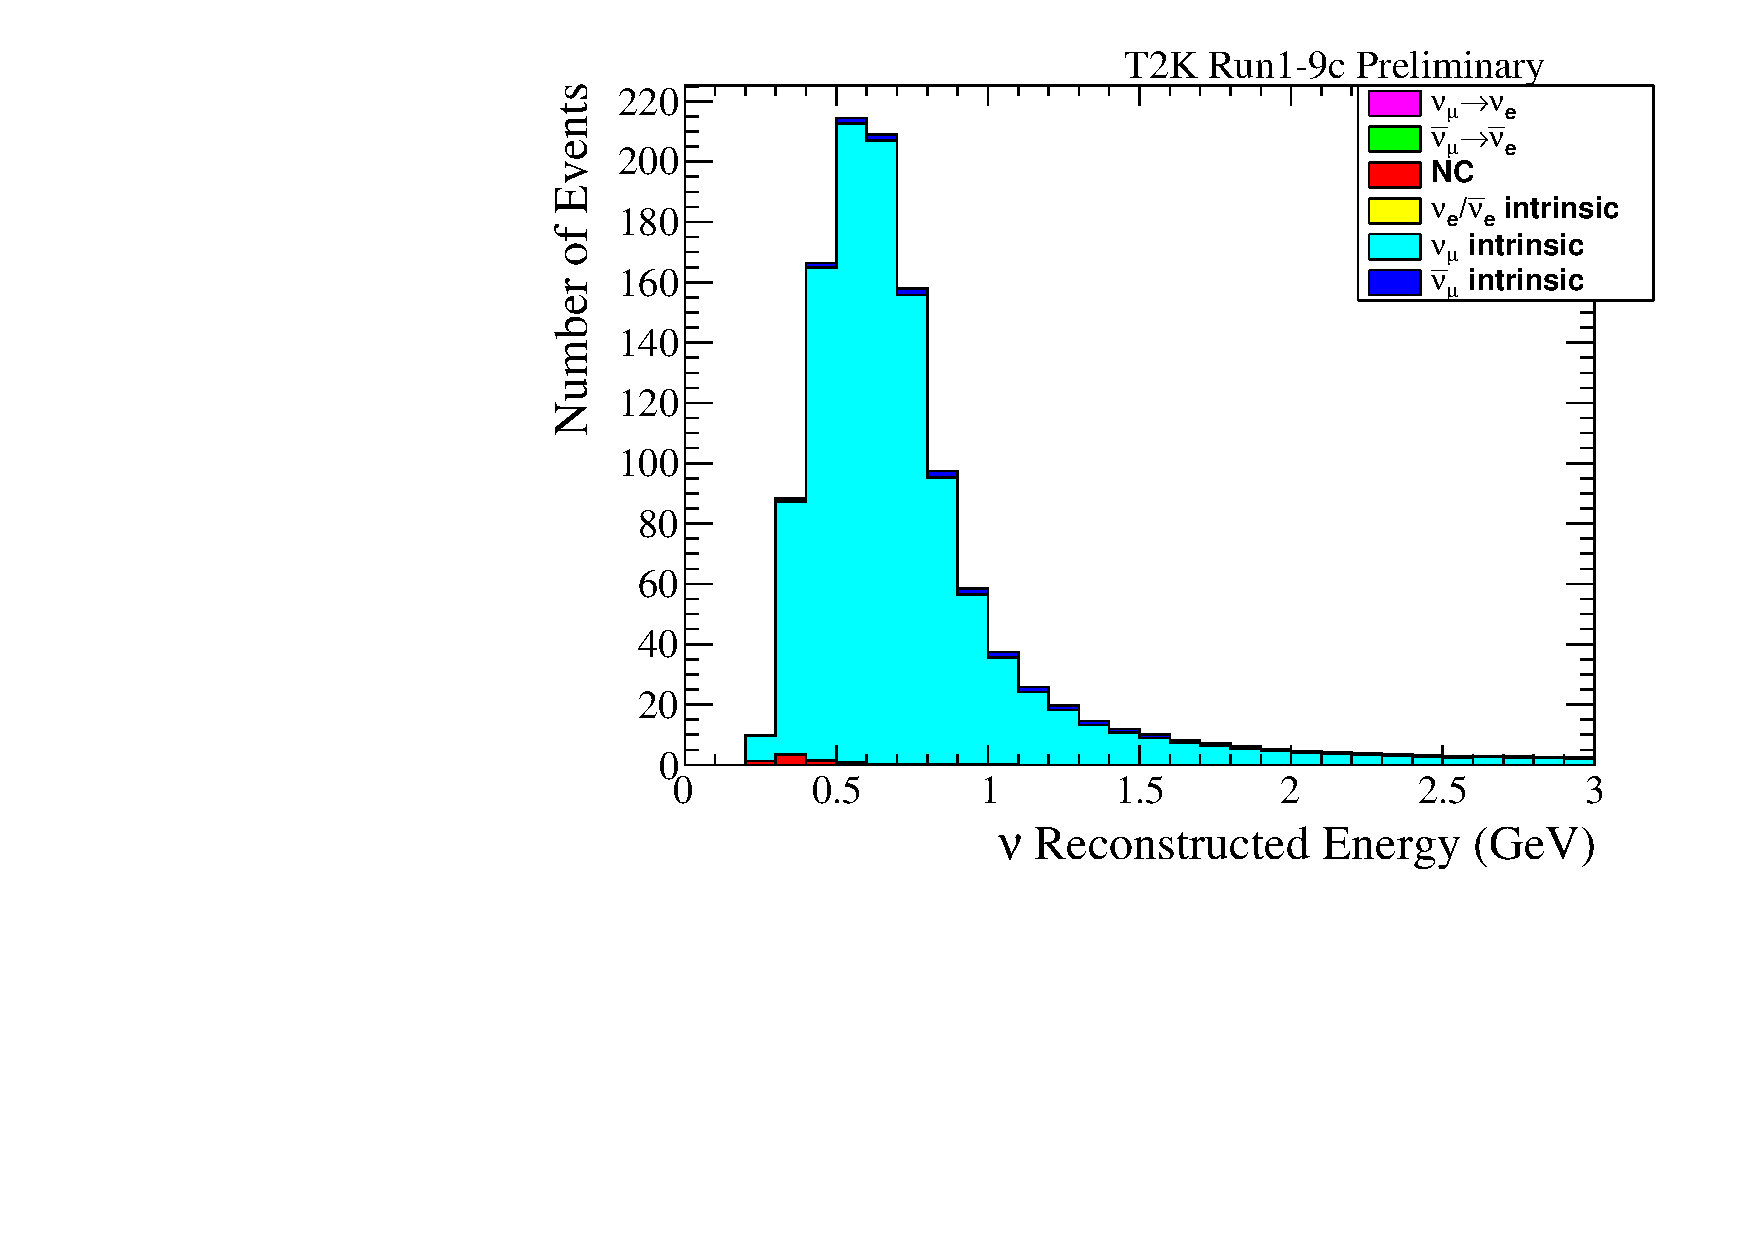
\includegraphics[width=0.9\textwidth]{images/spectra/unosc/spectrum_unosc_1Rmu}
		\caption{Muon-like, neutrino mode}
	\end{subfigure}
	\begin{subfigure}[b]{0.49\textwidth}
		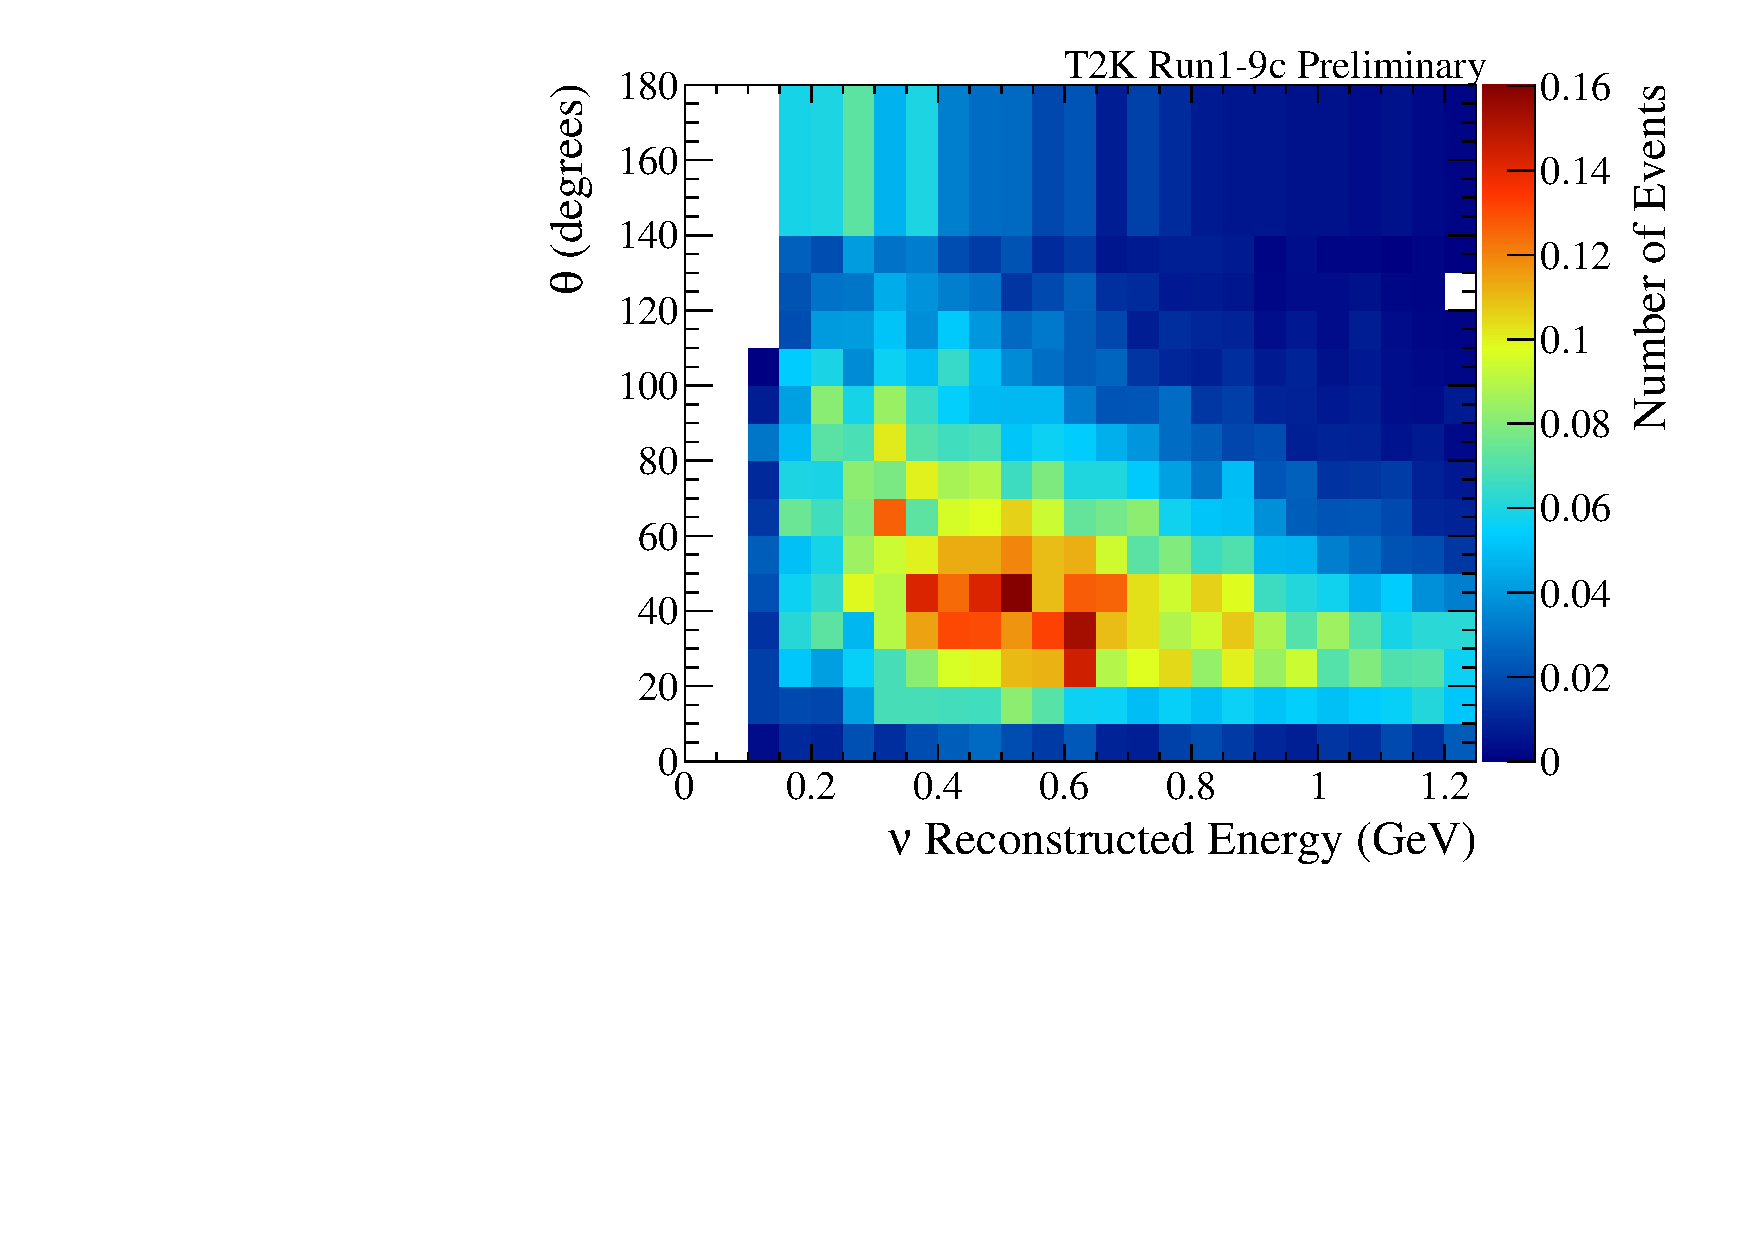
\includegraphics[width=0.9\textwidth]{images/spectra/unosc/spectrum_unosc_1Re}
		\caption{Electron-like, neutrino mode}
	\end{subfigure}
	\begin{subfigure}[b]{0.49\textwidth}
		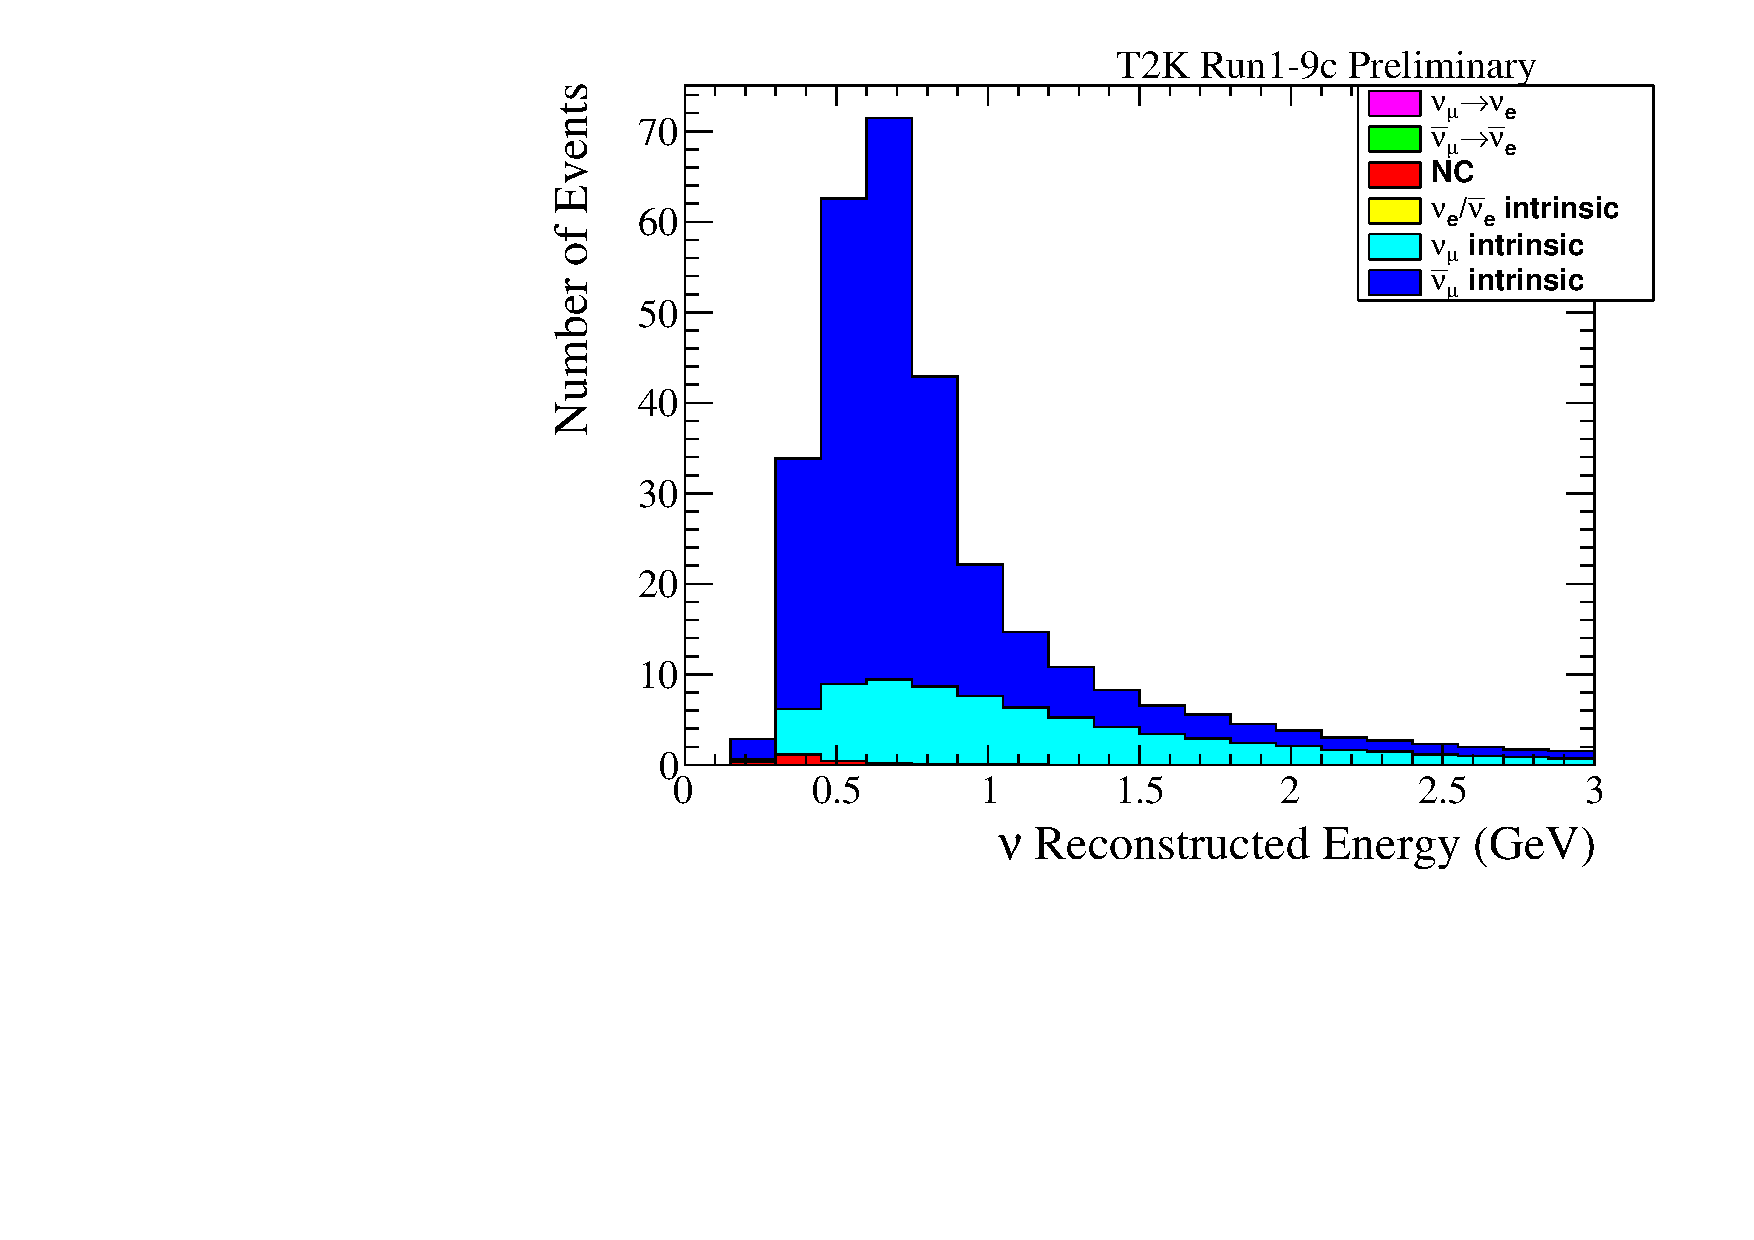
\includegraphics[width=0.9\textwidth]{images/spectra/unosc/spectrum_unosc_RHC1Rmu}
		\caption{Muon-like, antineutrino mode}
	\end{subfigure}
	\begin{subfigure}[b]{0.49\textwidth}
		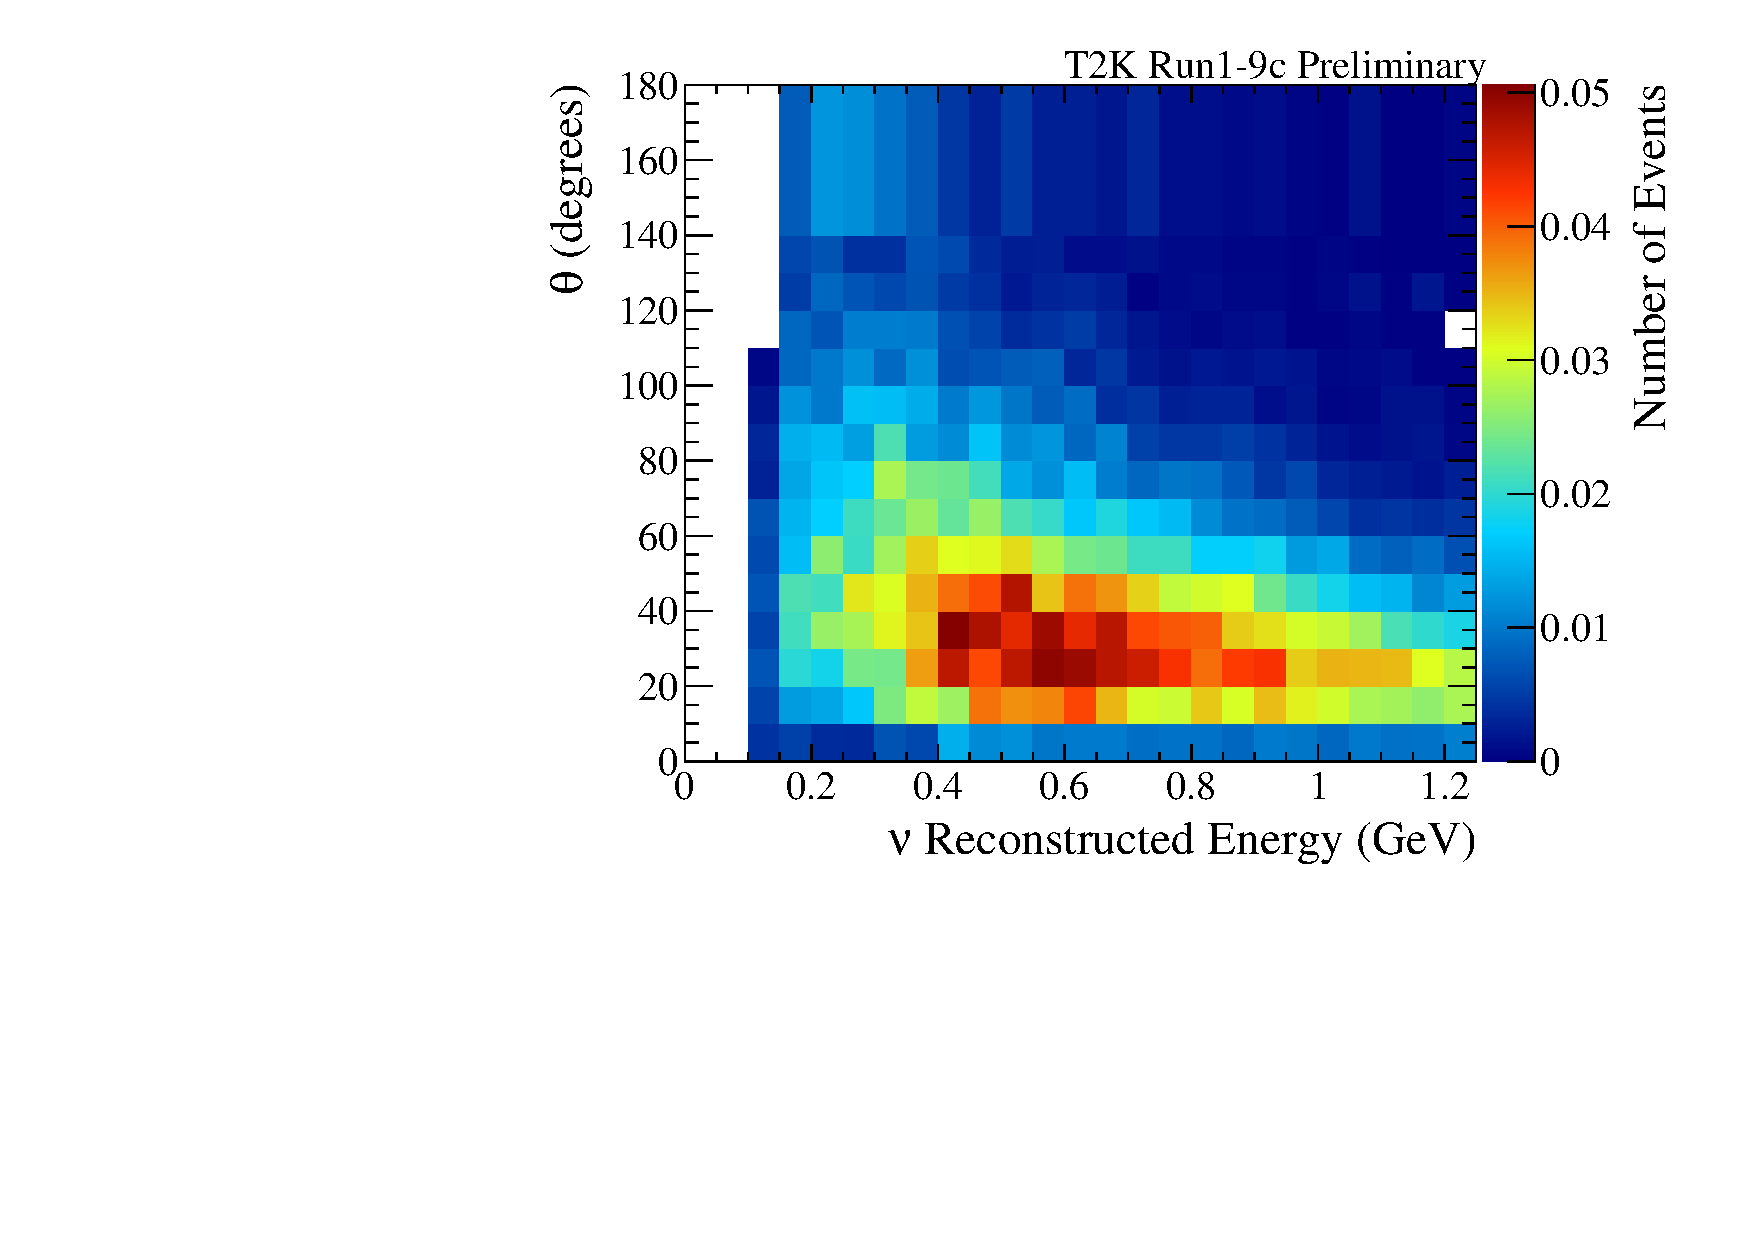
\includegraphics[width=0.9\textwidth]{images/spectra/unosc/spectrum_unosc_RHC1Re}
		\caption{Electron-like antineutrino mode}
	\end{subfigure}
	\begin{subfigure}[b]{0.49\textwidth}
		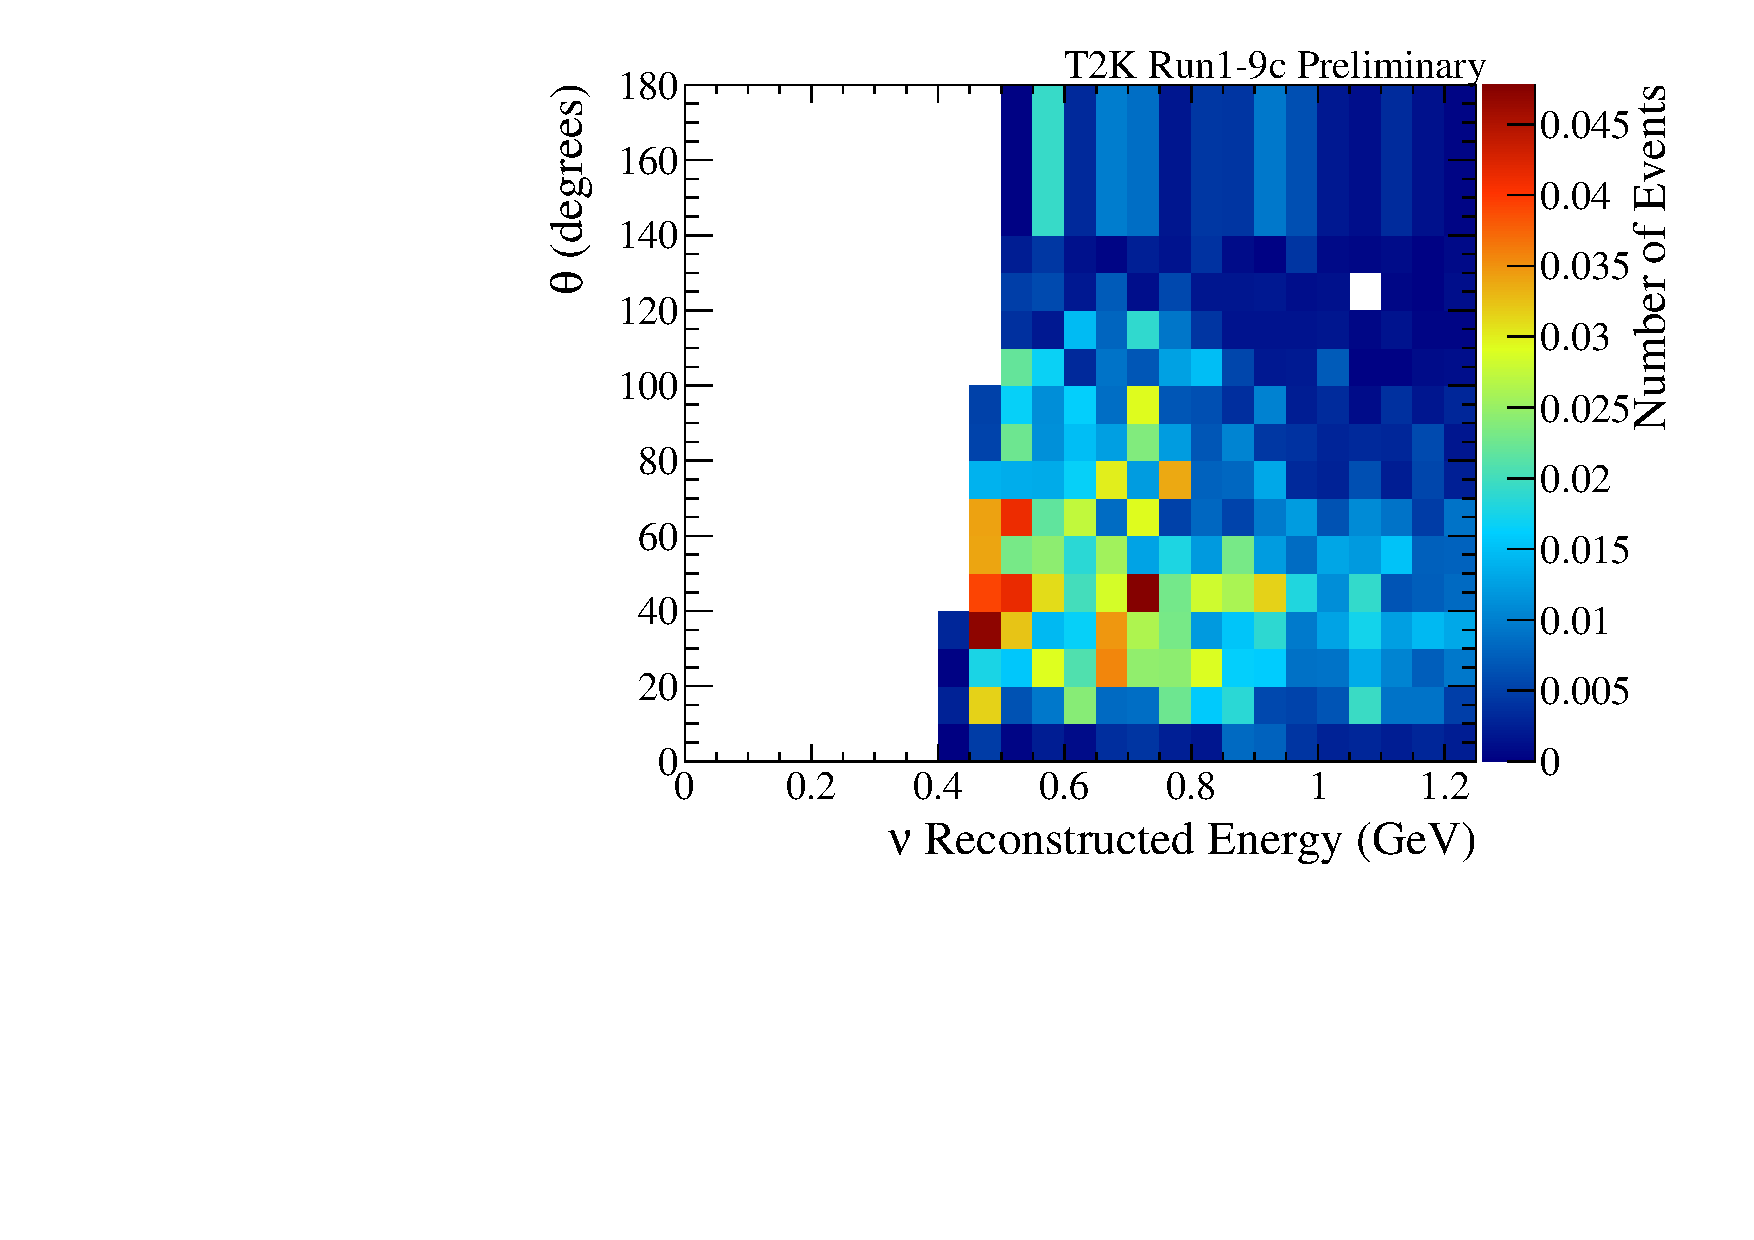
\includegraphics[width=0.9\textwidth]{images/spectra/unosc/spectrum_unosc_MultiRe}
		\caption{\nueCConepi-like, neutrino mode}
	\end{subfigure}
	\caption {
		Predicted unoscillated spectra. $\mu$-like distributions are a function of the reconstructed neutrino energy, while the $e$-like, including \nueCConepi, distributions are functions of both the reconstructed neutrino energy and the reconstructed angle between the outgoing lepton and the neutrino direction. The distributions correspond to the statistics collected in the full \RunPeriod data set. The spectra are generated with the systematic parameters described in \cref{sec:systematics}.
	}
	\label{fig:unosc_spectra_all}
\end{figure*}
\clearpage
\begin{figure*}[htb]
	\center
	\begin{subfigure}[b]{0.49\textwidth}
		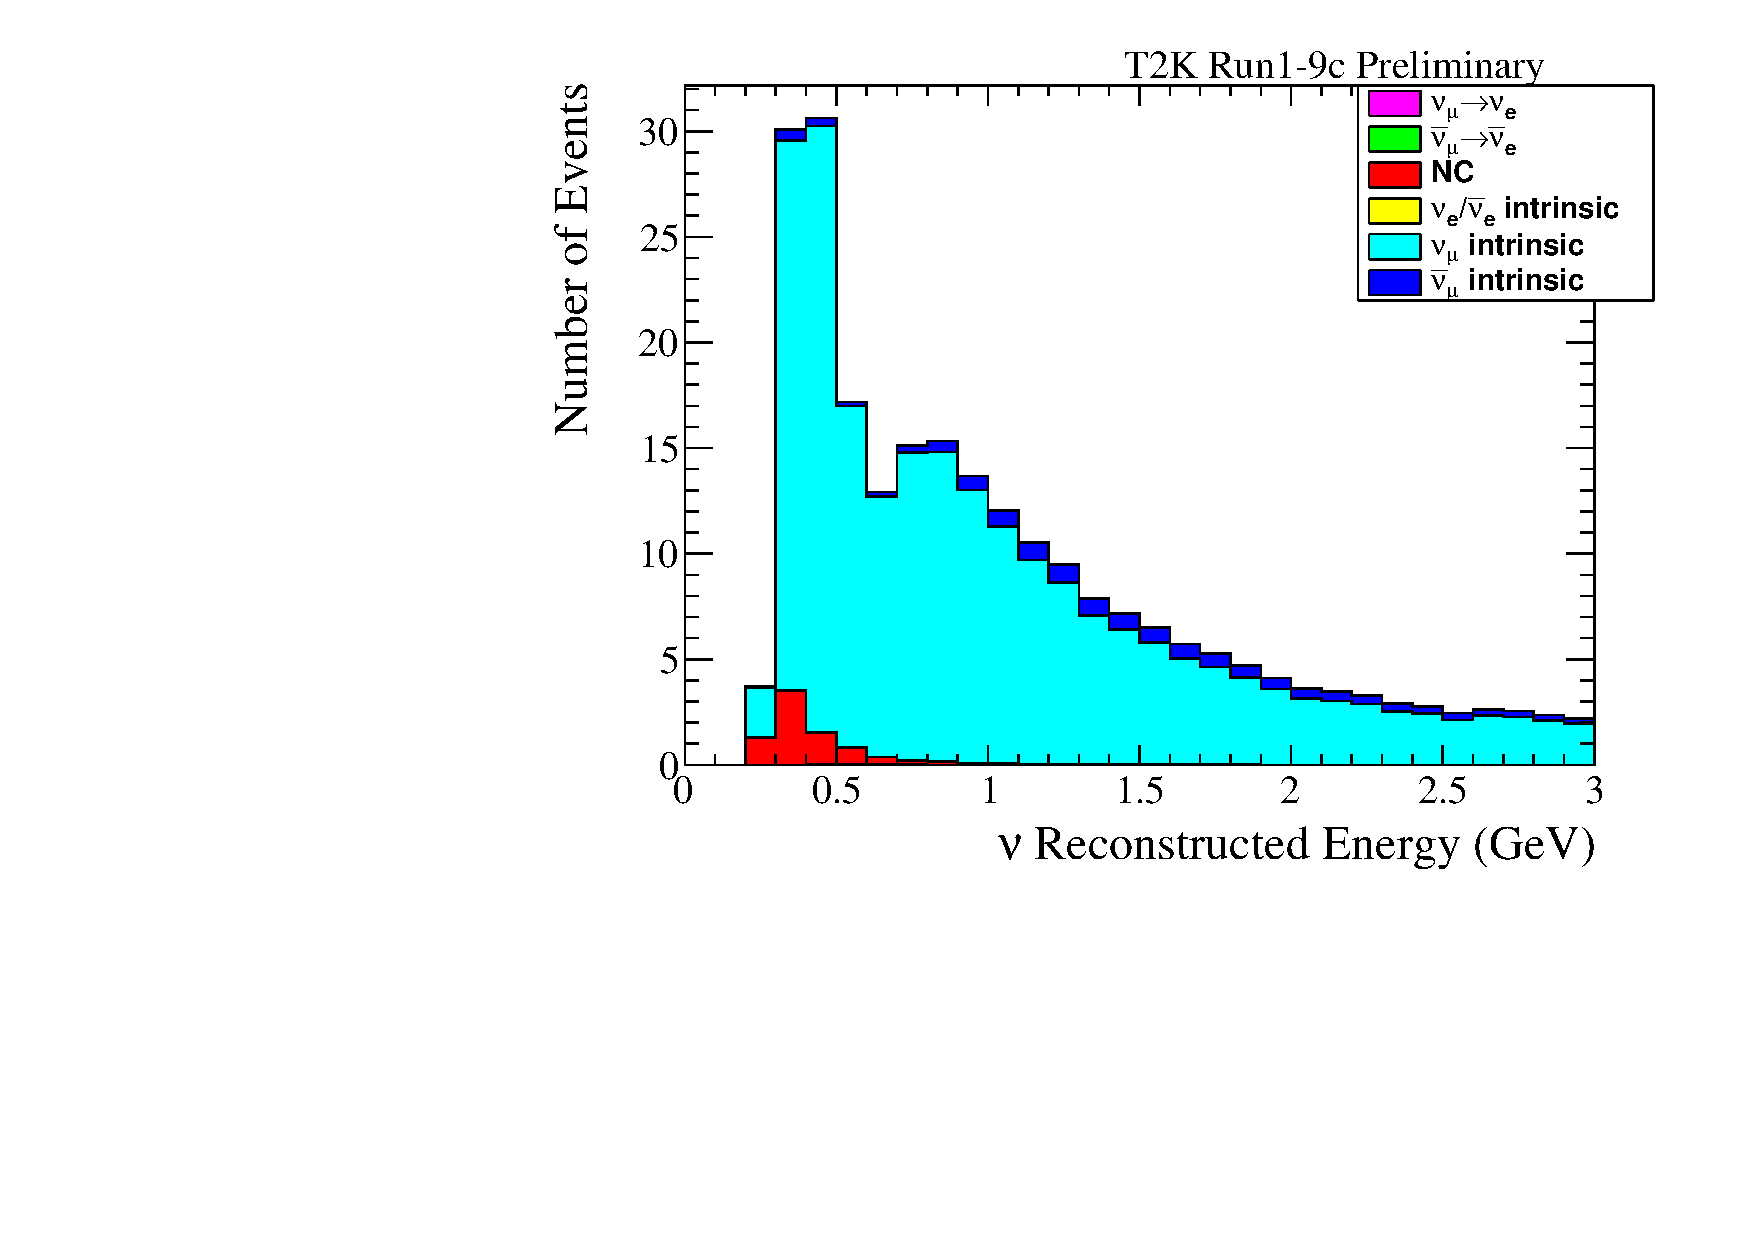
\includegraphics[width=0.9\textwidth]{images/spectra/asimova/spectrum_asimova_1Rmu}
		\caption{Muon-like, neutrino mode}
	\end{subfigure}
	\begin{subfigure}[b]{0.49\textwidth}
		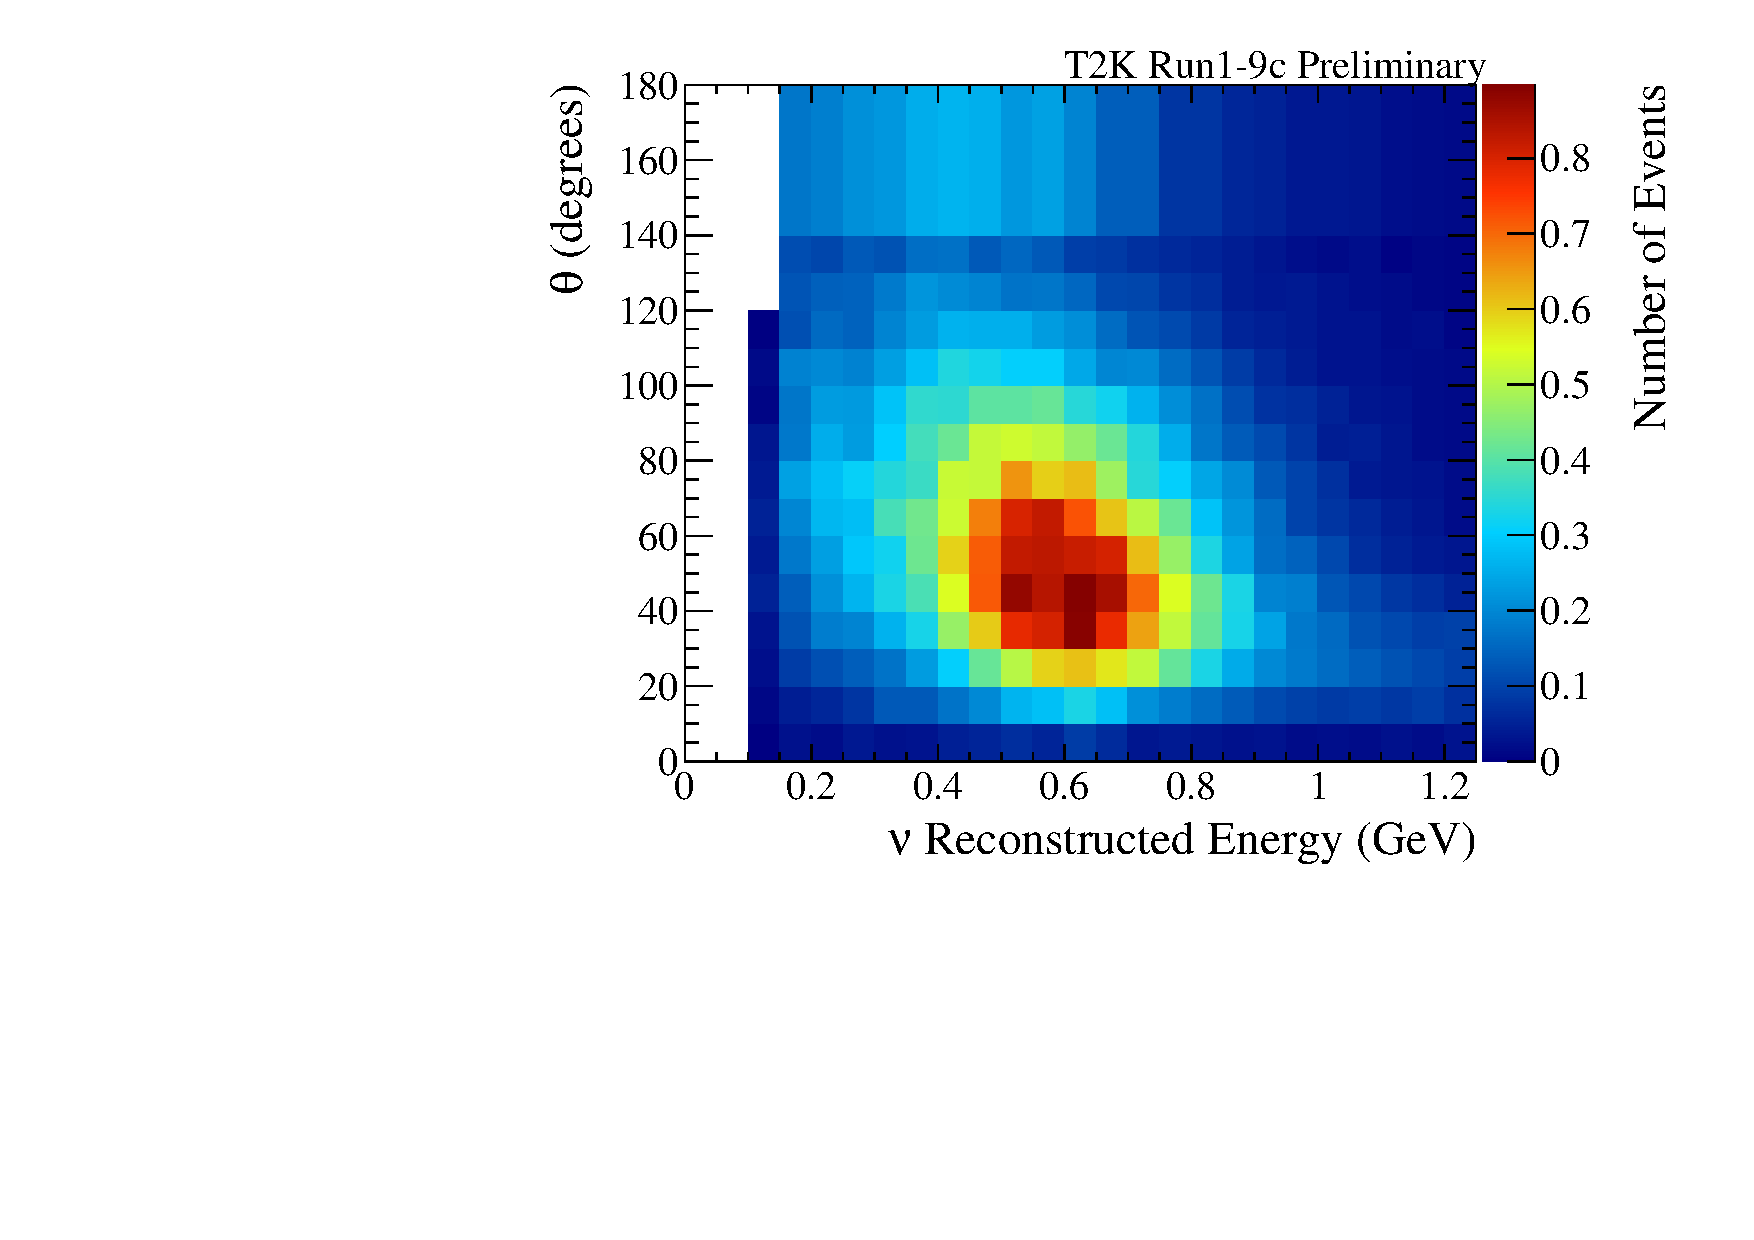
\includegraphics[width=0.9\textwidth]{images/spectra/asimova/spectrum_asimova_1Re}
		\caption{Electron-like, neutrino mode}
	\end{subfigure}
	\begin{subfigure}[b]{0.49\textwidth}
		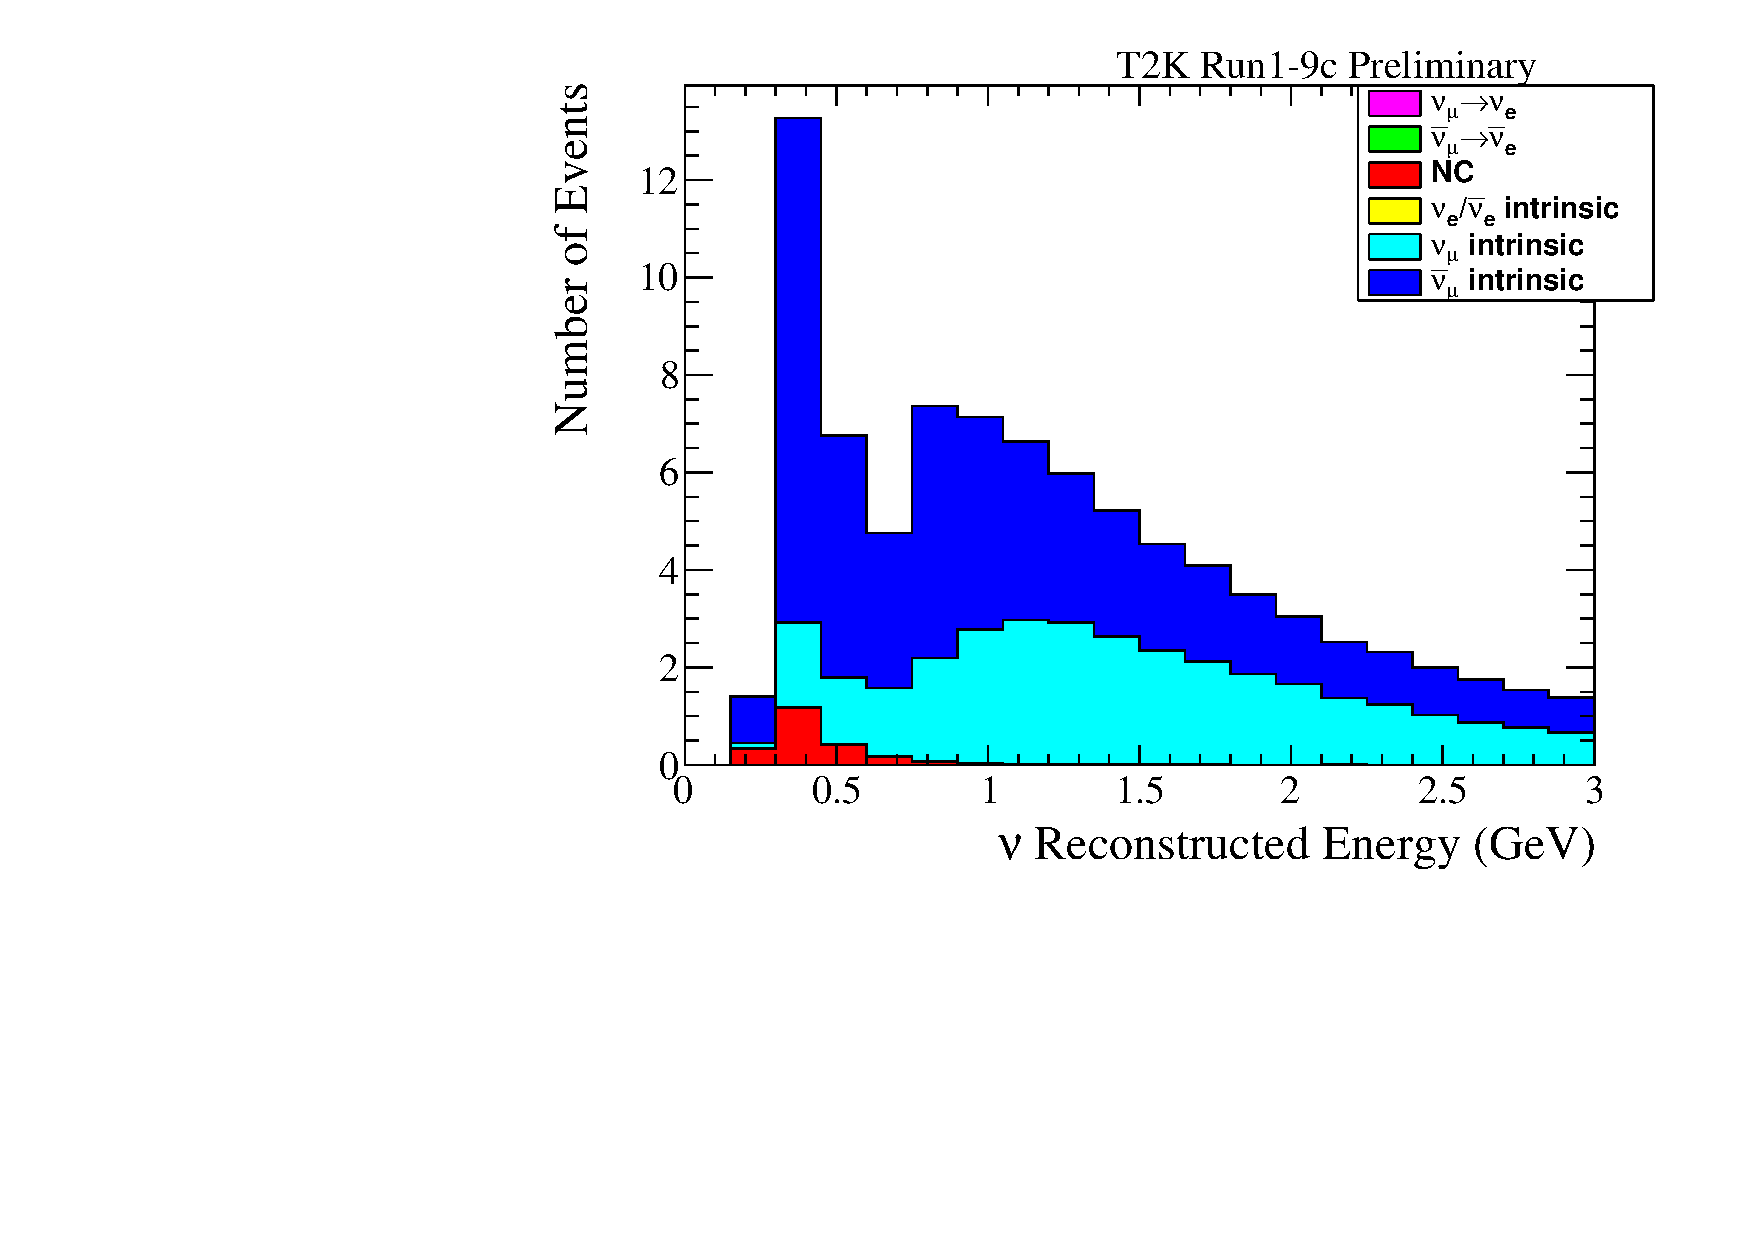
\includegraphics[width=0.9\textwidth]{images/spectra/asimova/spectrum_asimova_RHC1Rmu}
		\caption{Muon-like, antineutrino mode}
	\end{subfigure}
	\begin{subfigure}[b]{0.49\textwidth}
		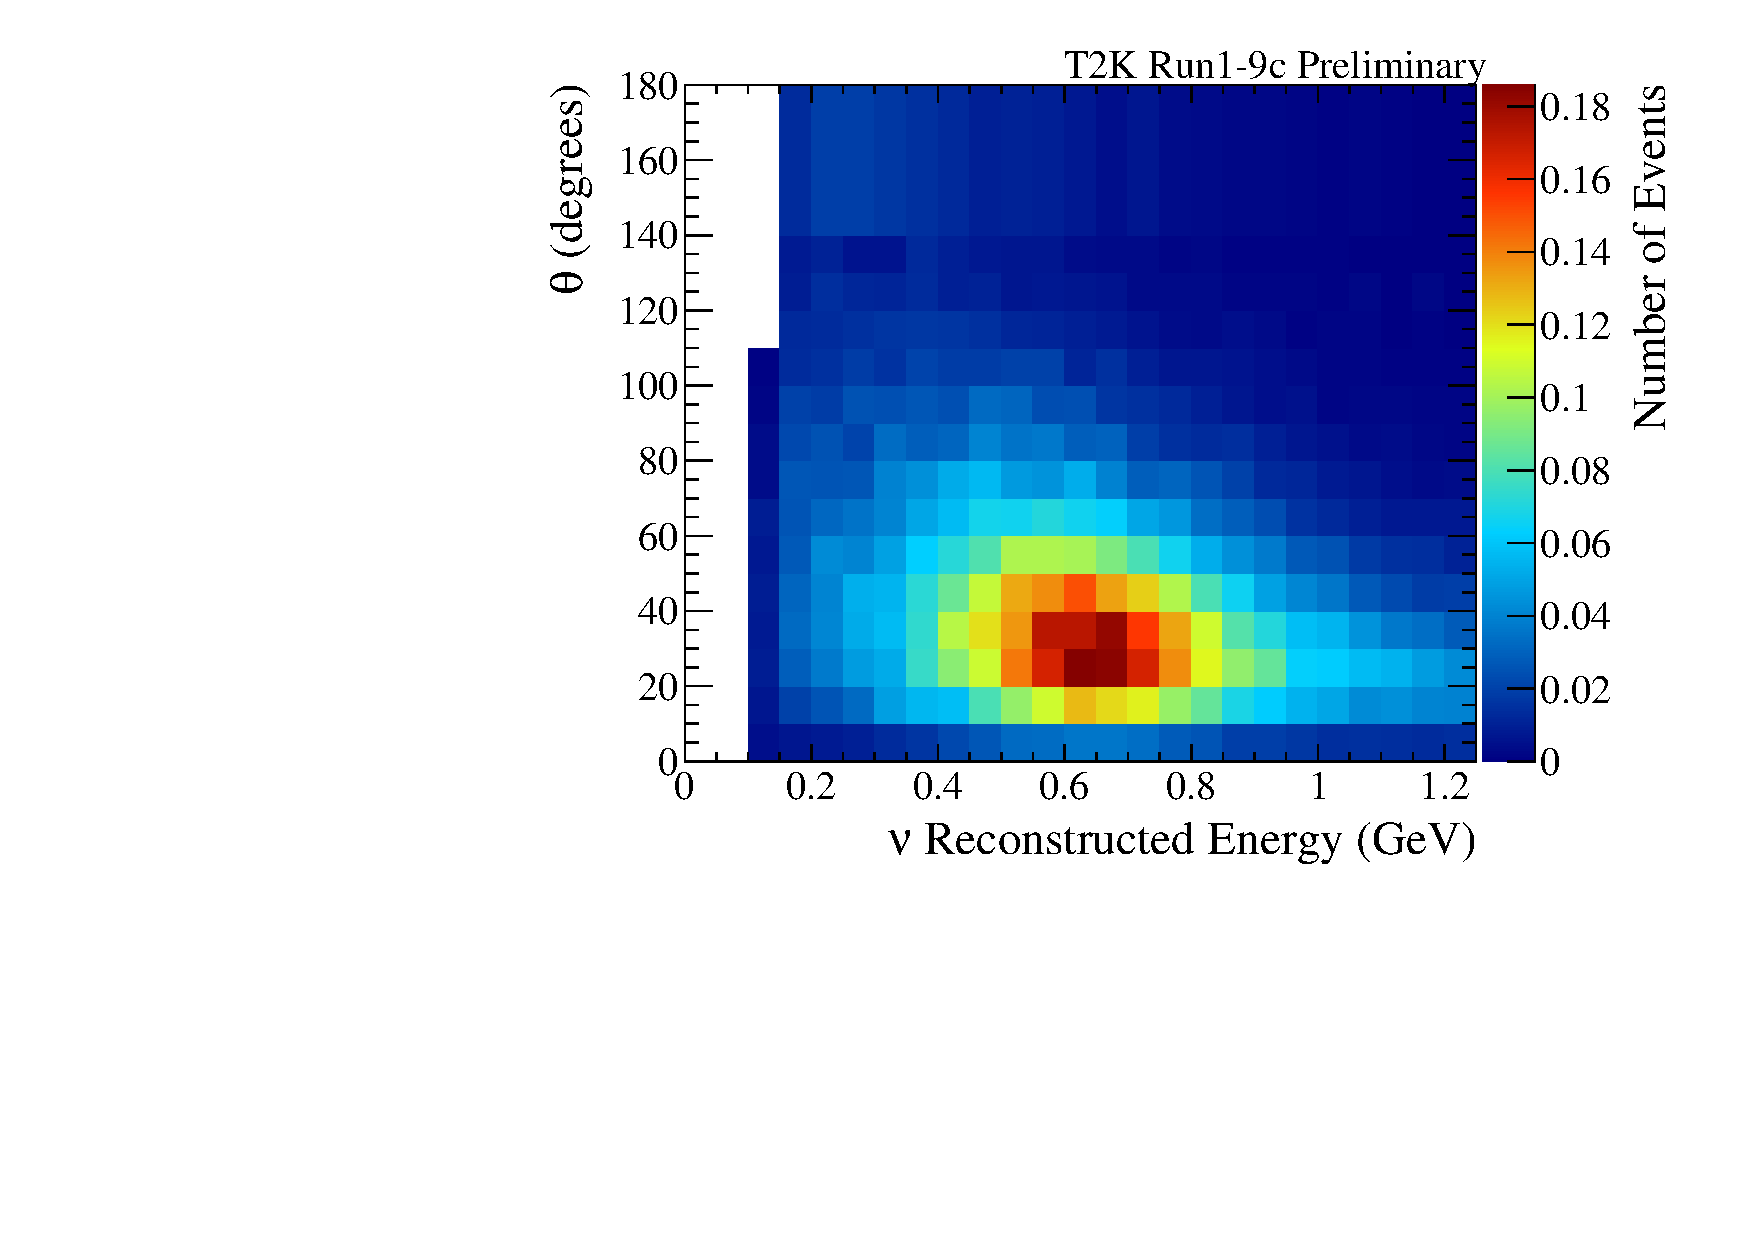
\includegraphics[width=0.9\textwidth]{images/spectra/asimova/spectrum_asimova_RHC1Re}
		\caption{Electron-like antineutrino mode}
	\end{subfigure}
	\begin{subfigure}[b]{0.49\textwidth}
		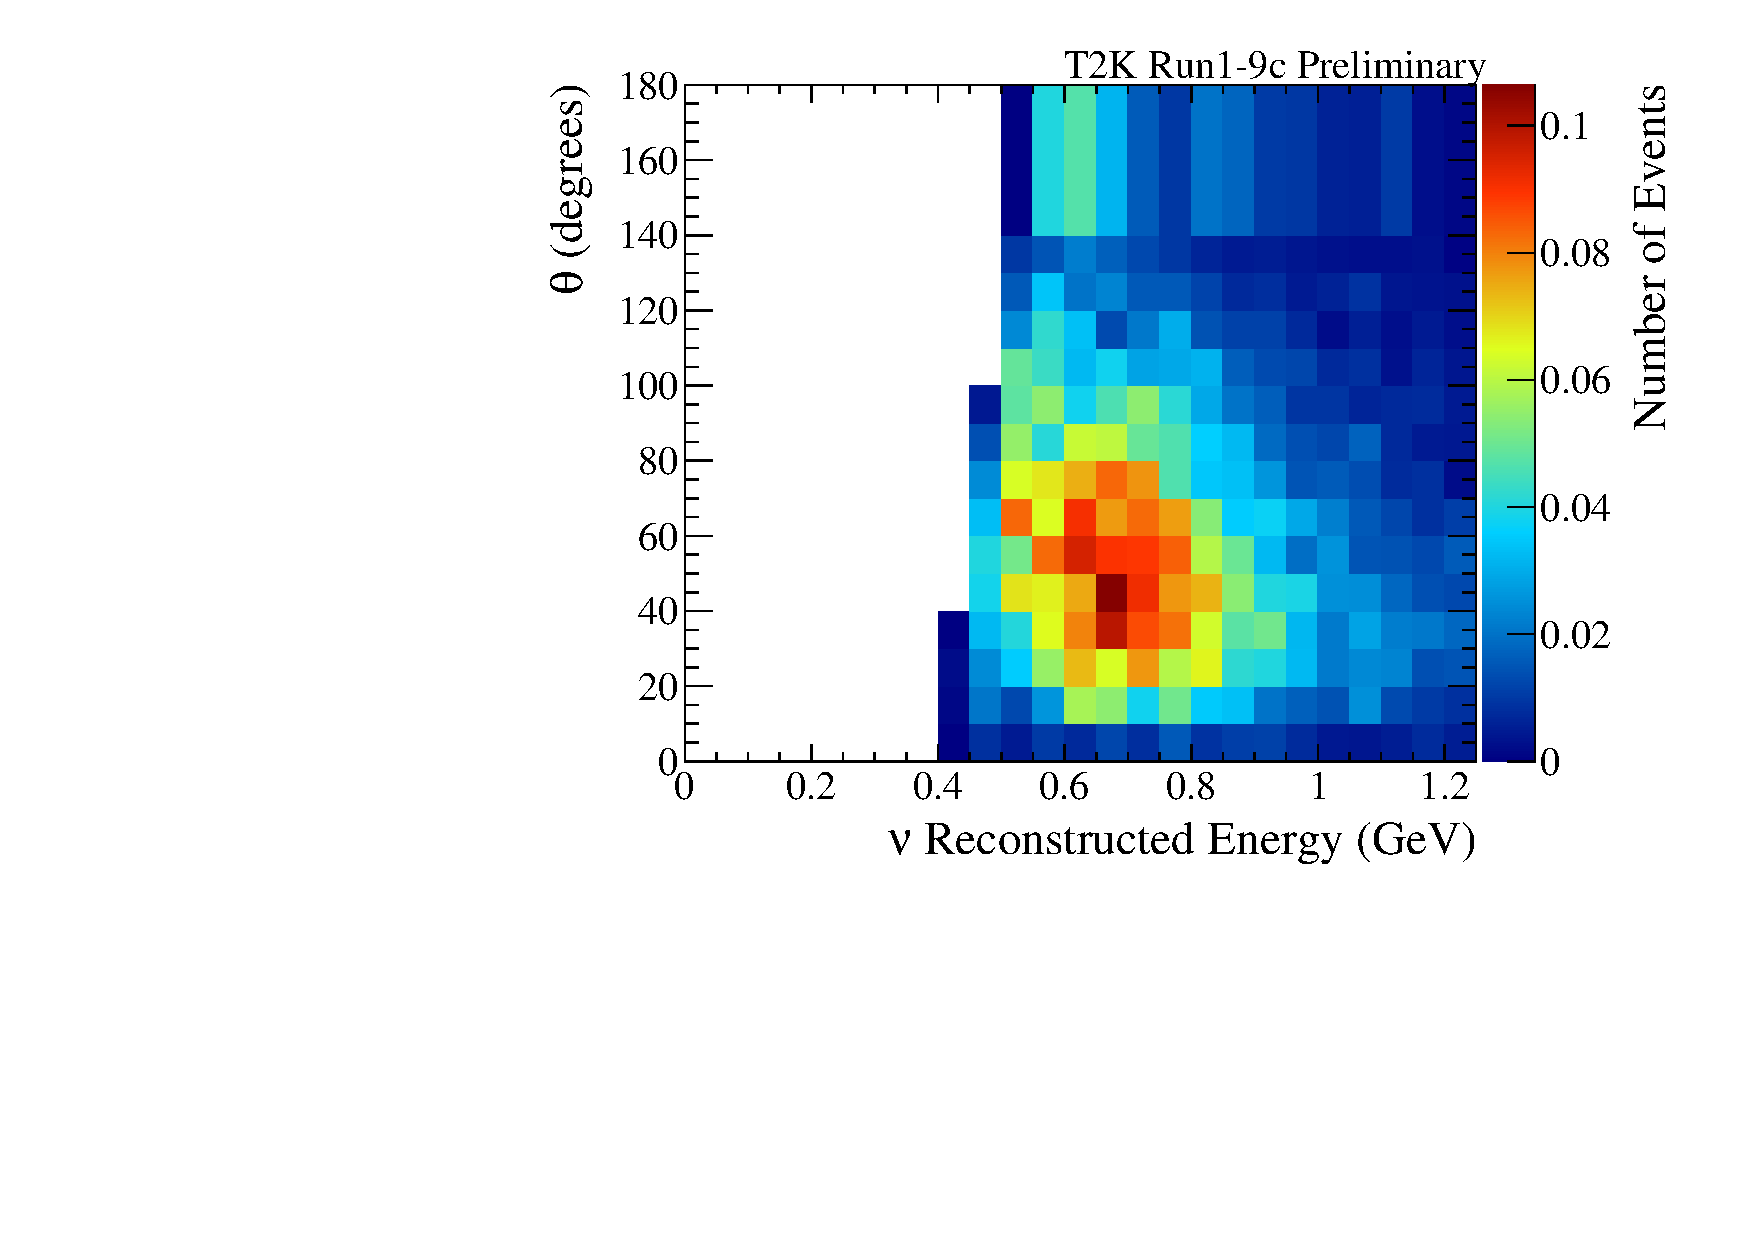
\includegraphics[width=0.9\textwidth]{images/spectra/asimova/spectrum_asimova_MultiRe}
		\caption{\nueCConepi-like, neutrino mode}
	\end{subfigure}
	\caption {
		Predicted Asimov A spectra. $\mu$-like distributions are a function of the reconstructed neutrino energy, while the $e$-like, including \nueCConepi, distributions are functions of both the reconstructed neutrino energy and the reconstructed angle between the outgoing lepton and the neutrino direction. The distributions correspond to the statistics collected in the full \RunPeriod data set. The spectra are generated with the systematic parameters described in \cref{sec:systematics} and the oscillation parameters corresponding to the Asimov data set A shown in \cref{tab:asimov_definition1}.
	}
	\label{fig:asimova_spectra_all}
\end{figure*}
\clearpage
\clearpage

\section {Systematic effects in the prediction of energy spectra}
\label{sec:systematics}

The description of the systematic parameters in this analysis can be found in \cite{OurRun18JointAnalysis3Flavour} (Sec. 3), this section will present the pre- and post-BANFF flux and cross-section covariance matrices and the SK covariance matrix (including detector, FSI, SI and PN effects). A summary of the best-fit values and pre- and post-BANFF errors of all systematics can be found in \cref{app:systematics}.

\begin{figure*}[htb]
	\center
	\begin{subfigure}[b]{0.49\textwidth}
		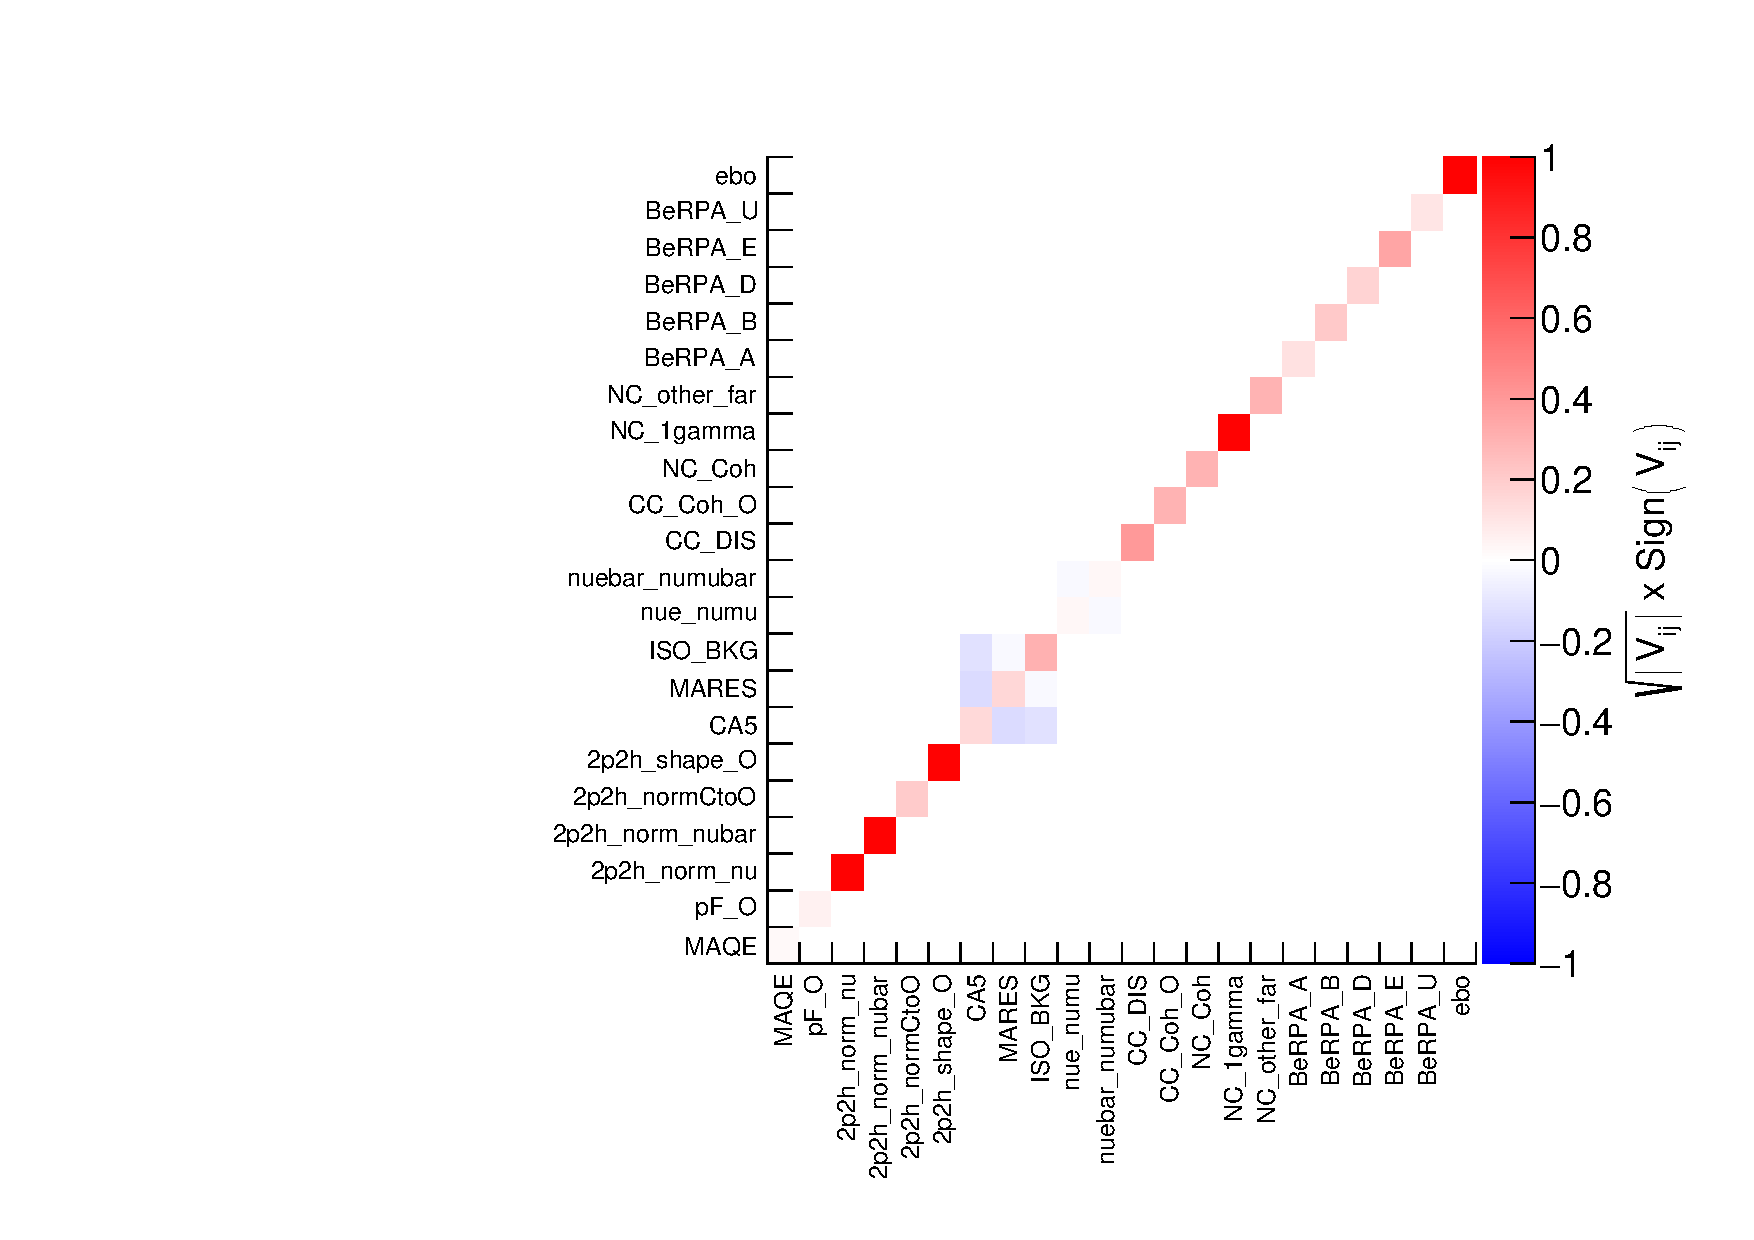
\includegraphics[width=\textwidth]{images/banff/xsec_prefit}
	\end{subfigure}
	\begin{subfigure}[b]{0.49\textwidth}
		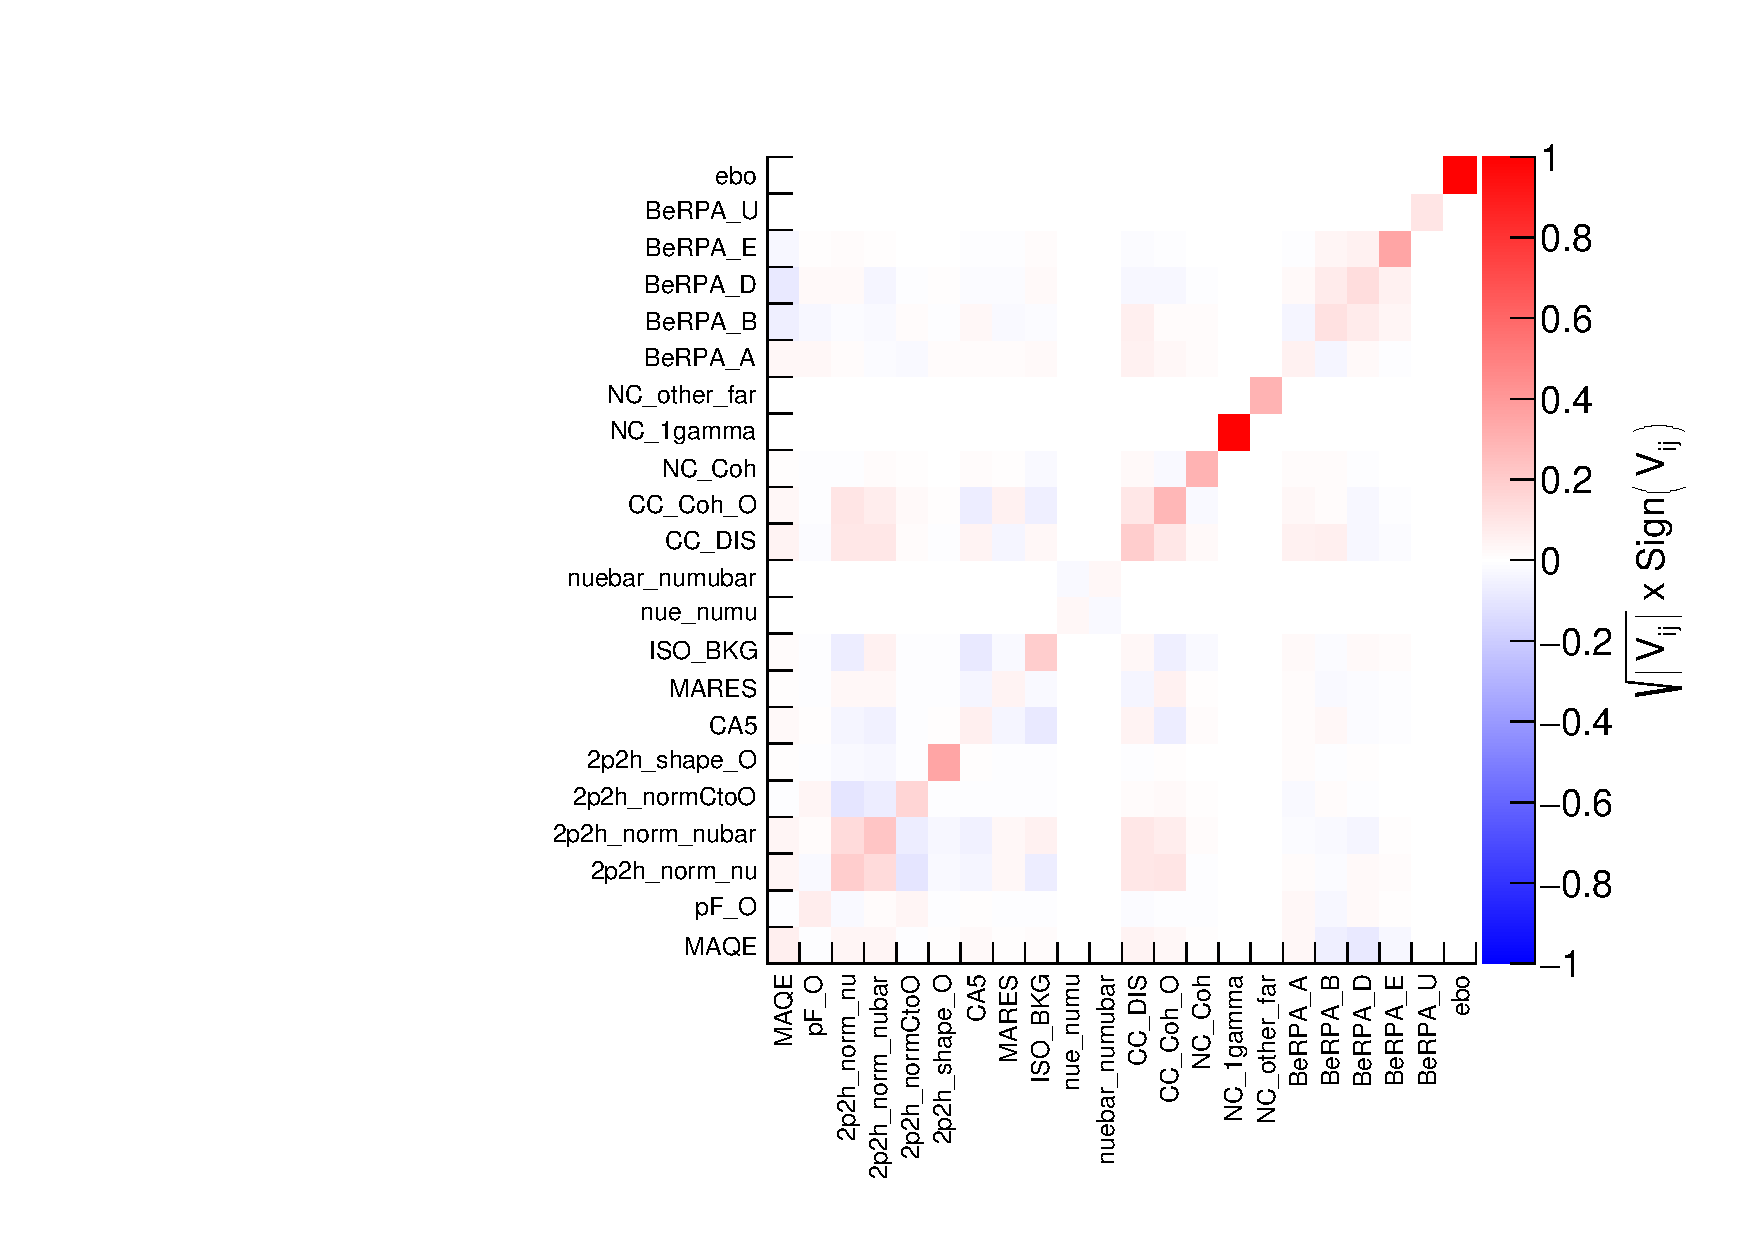
\includegraphics[width=\textwidth]{images/banff/xsec_postfit}
	\end{subfigure}
	\caption{The pre-BANFF (left) and post-BANFF (right) cross-section covariance matrix, with the values shown as the sign of the element times the square root of the absolute value of the element.}
	\label{fig:xsec_corr}
\end{figure*}

\begin{figure*}[htb]
	\center
	\begin{subfigure}[b]{0.7\textwidth}
		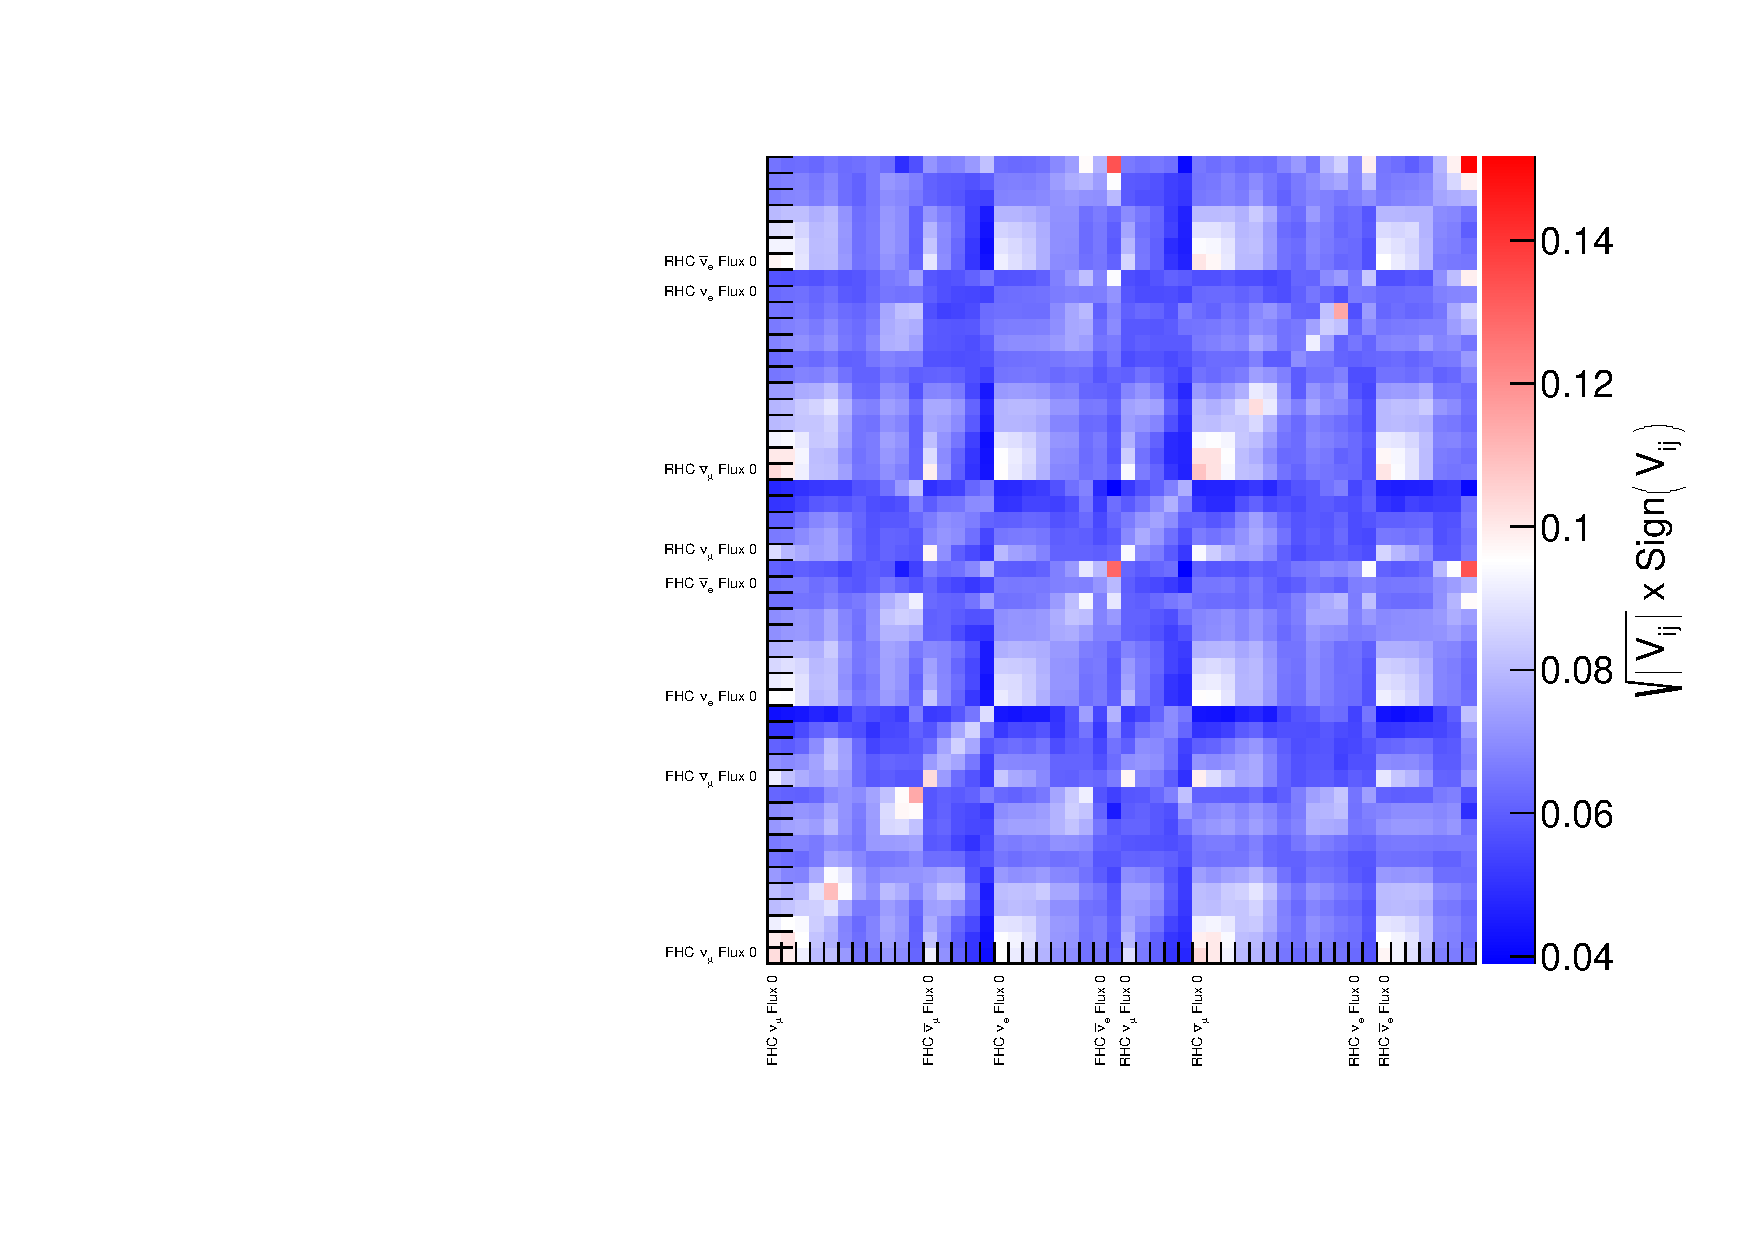
\includegraphics[width=\textwidth]{images/banff/flux_prefit}
	\end{subfigure}
	\begin{subfigure}[b]{0.7\textwidth}
		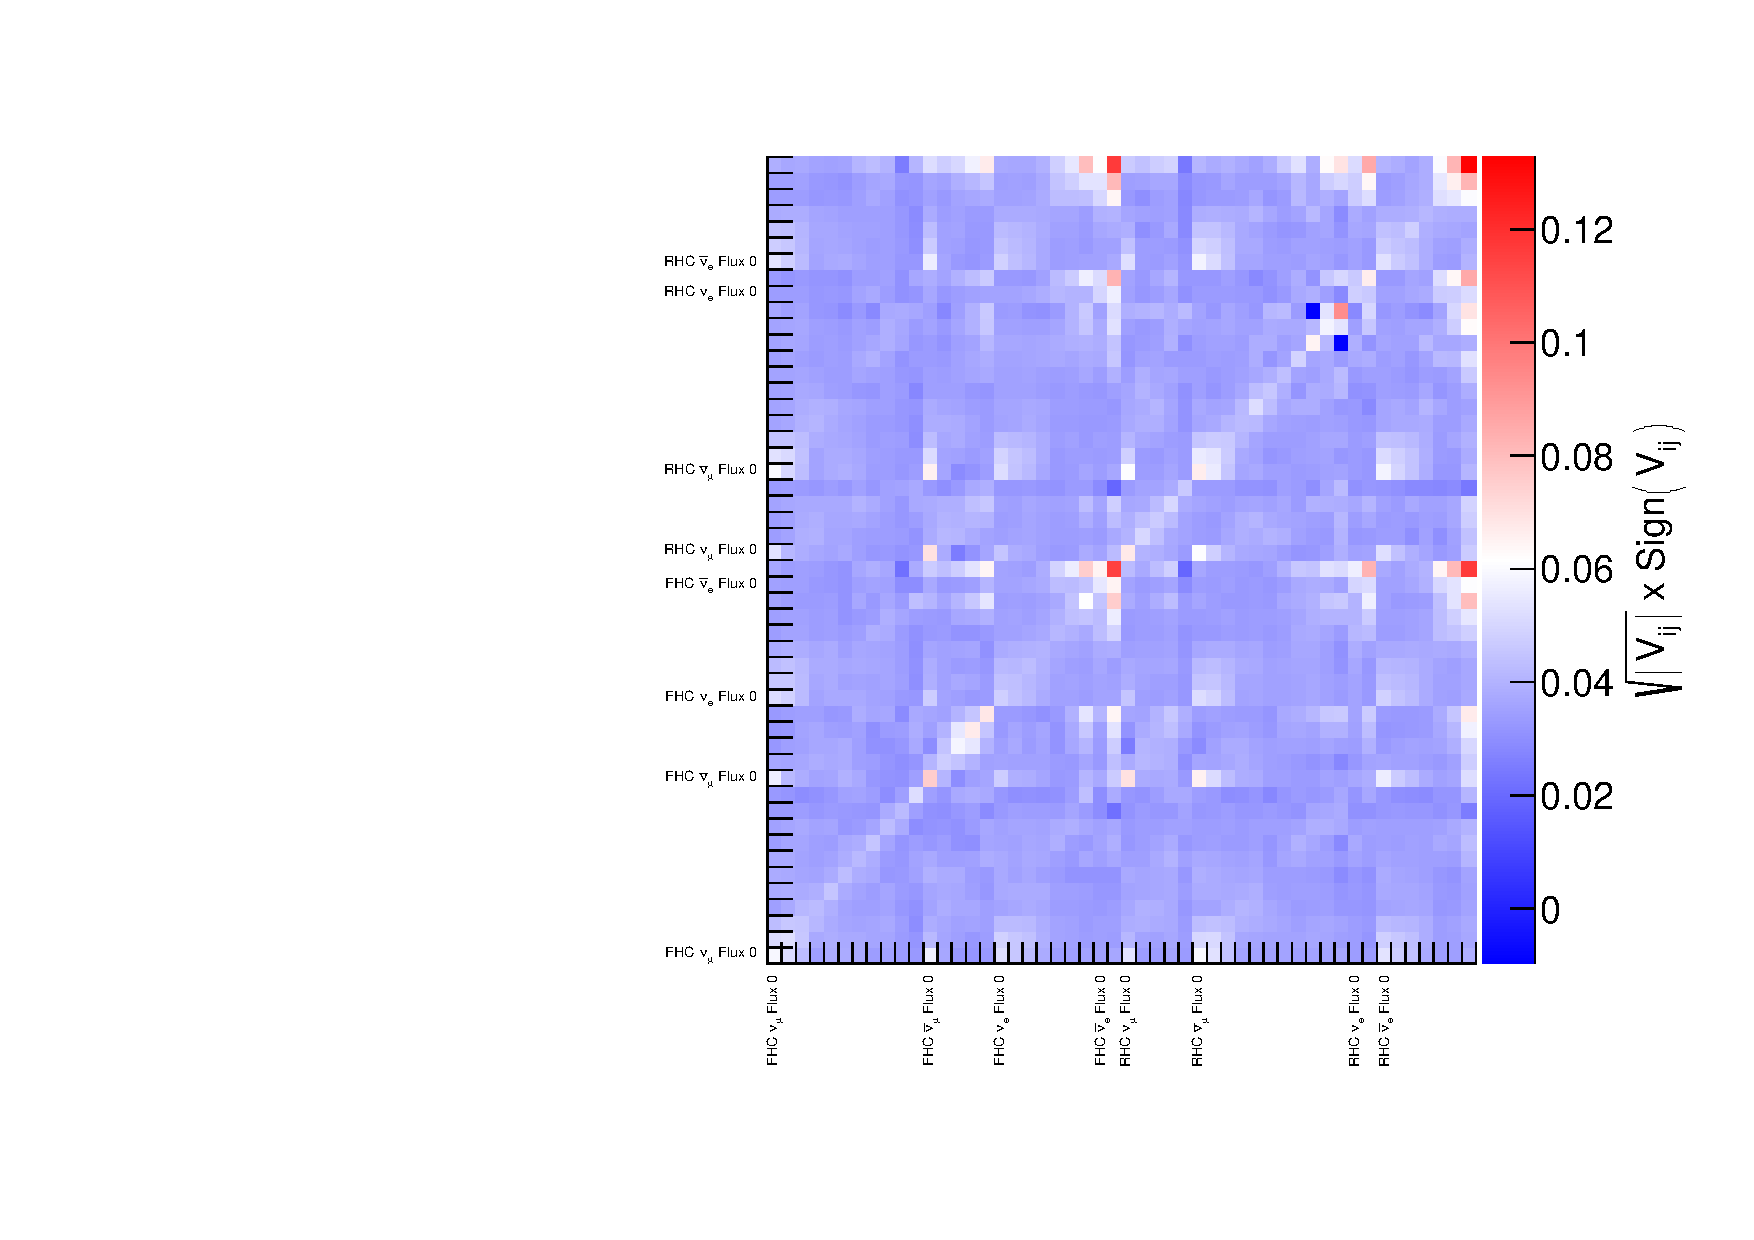
\includegraphics[width=\textwidth]{images/banff/flux_postfit}
	\end{subfigure}
	\caption{The pre-BANFF (top) and post-BANFF (bottom) flux covariance matrix, with the values shown as the sign of the element times the square root of the absolute value of the element.}
	\label{fig:flux_corr}
\end{figure*}

\begin{figure*}[htb]
	\center
	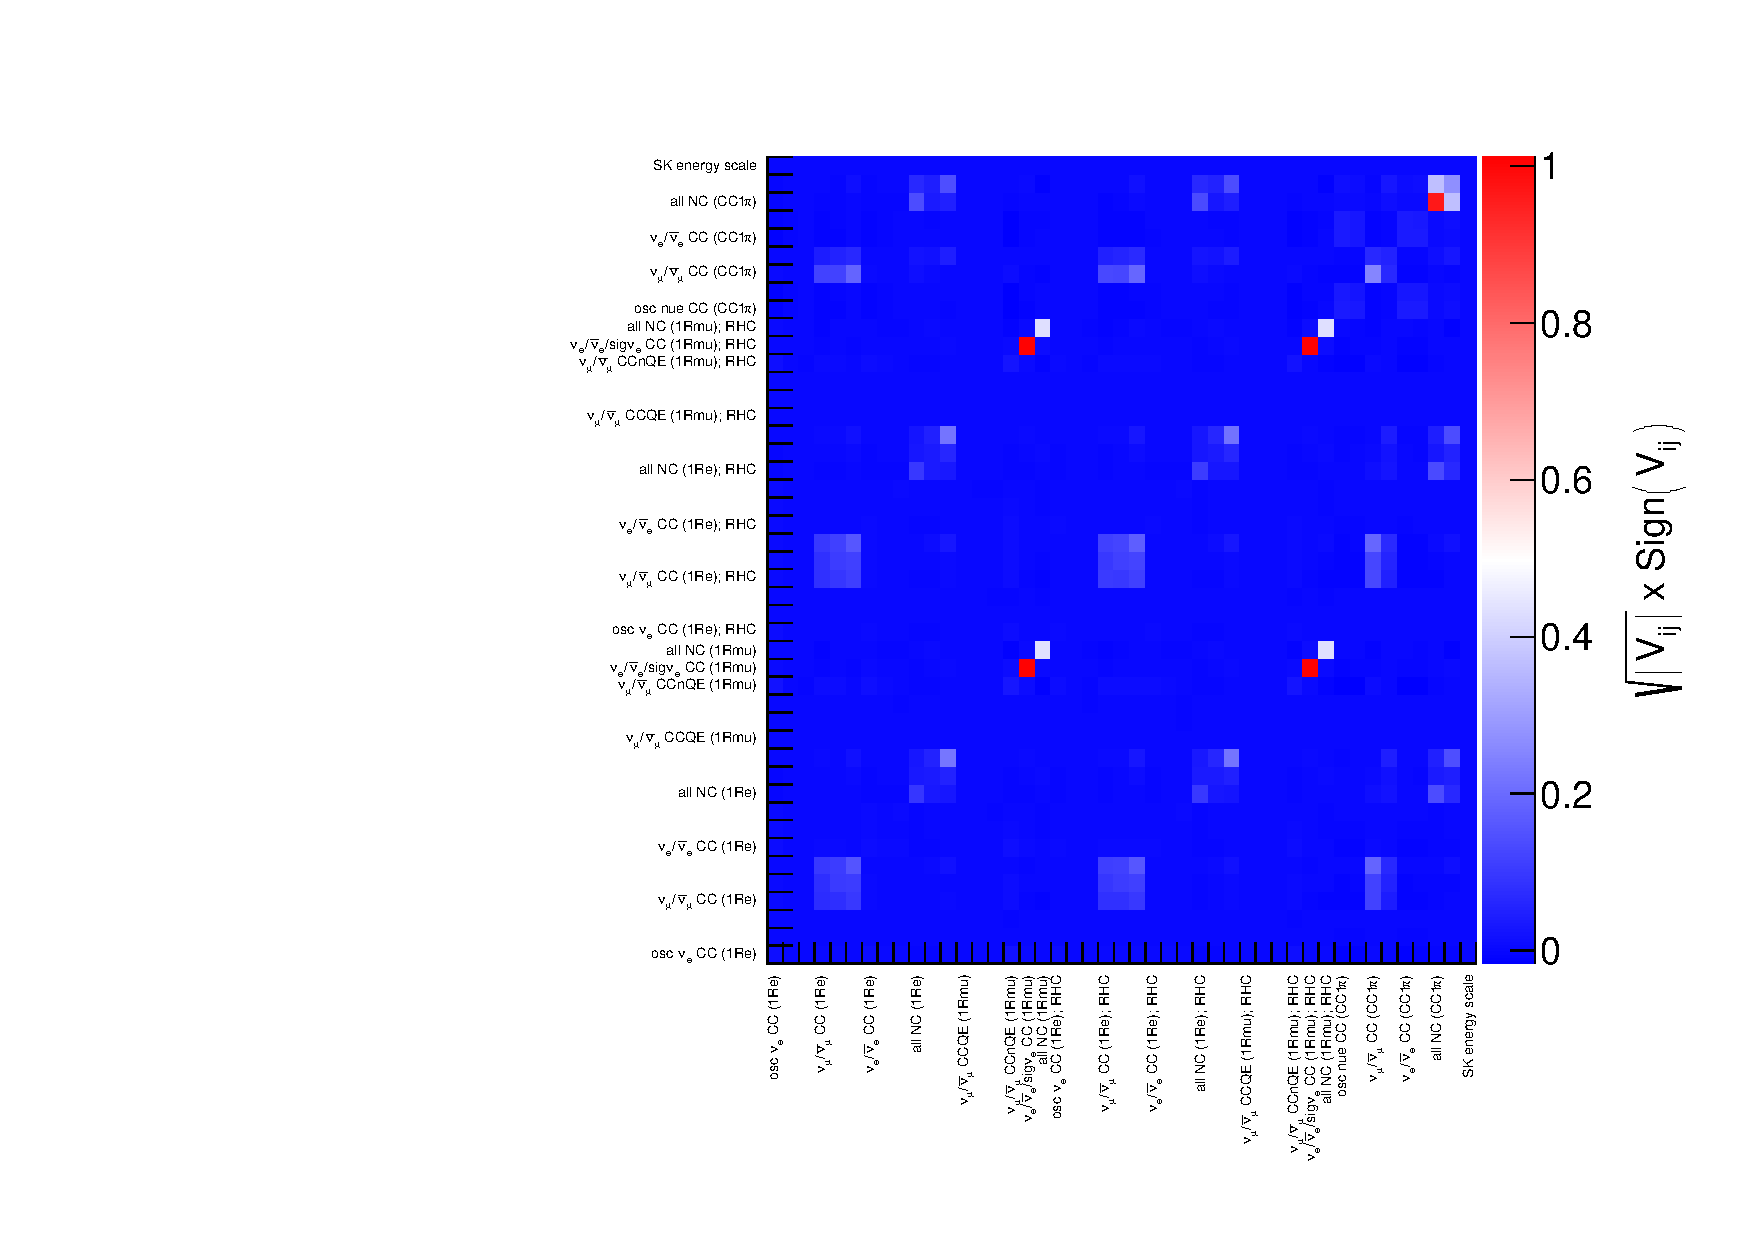
\includegraphics[width=\textwidth]{images/skdetfsi/skmatrix_tot}
	\caption{The SK covariance matrix, with the values shown as the sign of the element times the square root of the absolute value of the element.}
	\label{fig:sk_corr}
\end{figure*}

\FloatBarrier
\clearpage

\subsection{Oscillation parameters and mass hierarchy (7 parameters)}

The 3-flavour oscillation probability is used.  All the nuisance oscillation parameters, i.e. those parameters which are not shown in a given contour, are marginalised except the mass hierarchy which is fixed to either normal or inverted hierarchy.

For $\sin^2 \theta_{13}$ two different priors can be used, depending on whether the reactor constraint is applied, denoted as ``reactors", when applied and ``T2K only" when not applied.

\begin{table}[h]
	\centering
	\begin{tabular}{| c | c | c | c |}
 	\hline
Parameter(s)	& Prior		& Range    \\
\hline
$\sin^{2}\theta_{23}$	&  uniform 	& $[0.3; 0.7]$      \\
$\sin^{2} 2 \theta_{13}$ reactors		&  gaussian 		& $0.0857 \pm 0.0046$ 	\\
$\sin^{2} 2 \theta_{13}$ T2K only	   	&  uniform		& $[0.03; 0.2]$ 	\\
$\sin^{2} 2 \theta_{12}$  								&  gaussian 		& $0.846 \pm 0.021$ \\
$|$\dmsqtwothree$|$ (NH) / $|$\dmsqonethree$|$ (IH)      		&  uniform		& $ [2.3; 2.7] \times 10^{-3}~\mbox{eV}^2/\mbox{c}^4$		 \\
$\Delta m^{2}_{21}$      								&  gaussian 		& $(7.53 \pm 0.18) \times 10^{-5}~\mbox{eV}^2/\mbox{c}^4$		\\
$\delta_{CP}$                                               				&  uniform 	& $[-\pi; +\pi]$ \\
Mass Hierarchy										&  fixed 		& NH or IH \\  
\hline
\end{tabular}
\caption{
Treatment of the oscillation parameters in the $\nu/\bar{\nu}$ joint analysis. All the gaussian priors are from \cite{pdg_2014}. The parameter $\sin^{2} 2 \theta_{13}$ can be constrained with the measurement of reactor experiments using the gaussian prior, otherwise a uniform prior is used and the measurement relies only on the T2K data. The nominal values of $\sin^2 2 \theta_{13}$, $\sin^2 2 \theta_{12}$ and $\Delta m^2_{21}$ are from \cite{pdg_2014}, while all the other oscillation parameter values corresponds to the most probable values obtained by the Bayesian analysis on the T2K run 1-4 neutrino mode data \cite{T2KLongPaper}. The mass hierarchy is not marginalised but fixed to either NH or IH.
}
\label{tab:osc_param_priors}
\end{table}


\subsection{Systematic error on Super-K predictions}
\label{sec:systematics:errortables}

The effect of each category of systematic parameter on the expected event rate for Super-K sample is given in \cref{tab:sk_errors_summary}. The mean and RMS of \NumToysSmall throws of the respective systematics (with correlations taken into account) is computed for each sample and in the case of pre-BANFF and post-BANFF errors. When not measuring the effect of oscillation parameters variations, the oscillation parameters are fixed at Asimov A values (see \cref{sec:asimov_definition}).

For the measurement of $\delta_{CP}$ it is important to understand the effect of the systematic uncertainties on the ratio of the number of events between neutrino and antineutrino mode samples. If correlations do not reproduce the physics correctly, a fake asymmetry between neutrino and antineutrino oscillations can be seen. Furthermore, if correlations exist but are not taken into account, the measurement of $\delta_{CP}$ could be biased. The true value of $\delta_{CP}$ determines whether correlations or anti-correlations between systematic parameters have the greatest effect in hiding any oscillation asymmetry. In particular, if true $\delta_{CP} = \pm \pi/2$ then anti-correlation in the $e$-like samples could hide any oscillation asymmetry. Alternatively, in the case that true $\delta_{CP} \sim 0$ it is uncorrelated parameters that reduce the sensitivity to $\delta_{CP}$. The uncertainties on the ratios between neutrino and antineutrino mode events due to the systematic parameters are shown in \cref{tab:sk_errors_summary}. The most critical systematic parameters are $\sigma_{\nu_e}$ and $\sigma_{\bar{\nu}_e}$ which are applied respectively to $\nu_e$ and $\bar{\nu}_e$ events. Their fractional error from the BANFF covariance matrix is $\sim2.8$\% (see \cref{tab:sys_xsec_err}) and they are partially anti-correlated with non-diagonal elements in the covariance matrix of -0.0004.

It can be seen in \crefrange{tab:sk_errors_1Rmu}{tab:sk_errors_MultiRe} (\Cref{app:systematics}) that the reduction in the error on flux and constrained cross-section systematics achieved through the BANFF fit reduces the fractional error due to all systematics from $\sim 14\%$ to $\sim 5\%$ and $\sim 12\%$ to $\sim 4\%$ in the neutrino- and antineutrino-mode $\mu$-like samples respectively, from $\sim 17\%$ to $\sim 9\%$ and $\sim 14\%$ to $\sim 7\%$ in the neutrino- and antineutrino-mode $e$-like samples respectively, and from $\sim 22\%$ to $\sim 18\%$ in the \nueCConepi{}-like sample.

\begin{table}[H]
	\centering
	\begin{tabular}{|l||l|l||l|l|l|l|l|}
		\hline
		& \multicolumn{2}{c||}{\textbf{1-Ring $\mu$}} & \multicolumn{4}{c|}{\textbf{1-Ring $e$}} \\ \hline
		Error source & FHC & RHC & FHC & RHC & FHC 1 d.e. & FHC/RHC \\ \hline\hline
		SK Detector & 2.40 & 2.01 & 2.83 & 3.79 & 13.16 & 1.47 \\ \hline
		SK FSI+SI+PN & 2.20 & 1.98 & 3.02 & 2.31 & 11.44 & 1.58 \\ \hline
		Flux + Xsec constrained & 2.88 & 2.68 & 3.02 & 2.86 & 3.82 & 2.31 \\ \hline
		E$_\text{b}$ & 2.43 & 1.73 & 7.26 & 3.66 & 3.01 & 3.74 \\ \hline
		$\sigma(\nu_e)/\sigma(\bar{\nu}_e)$ & 0.00 & 0.00 & 2.63 & 1.46 & 2.62 & 3.03 \\ \hline
		NC1$\gamma$ & 0.00 & 0.00 & 1.07 & 2.58 & 0.33 & 1.49 \\ \hline
		NC Other & 0.25 & 0.25 & 0.14 & 0.33 & 0.99 & 0.18 \\ \hline
		Osc & 0.03 & 0.03 & 3.86 & 3.60 & 3.77 & 0.79 \\ \hline\hline
		All Systematics & 4.91 & 4.28 & 8.81 & 7.03 & 18.32 & 5.87 \\ \hline
		All with osc & 4.91 & 4.28 & 9.60 & 7.87 & 18.65 & 5.93 \\ \hline
	\end{tabular}
	\caption
	{
	Percentage error on event rate by error source and sample. Final column is the percentage error on the ratio of FHC/RHC events in the one-ring $e$ sample.
	}
	\label{tab:sk_errors_summary}
\end{table}


The error envelopes corresponding to \cref{tab:sk_errors_summary} are shown in \cref{app:systematics}.

\clearpage


%..................

%%% Local Variables:
%%% mode: latex
%%% TeX-master: "../TN327"
%%% End:

\clearpage

\section {Sensitivity studies}
\label{sec:sensitivity}
To determine the sensitivity of the analysis a number of fits were performed using Asimov data sets A and B, the contours for which indicate the ability of the analysis to measure the oscillation parameters in the absence of statistical fluctuations and under the assumption that their true values correspond to the Asimov values. Fits of single parameters are performed for each of \ssqthonethree, \deltacp, \ssqthtwothree and \dmsq (\dmsqtwothree in normal hierarchy and \dmsqonethree in inverted hierarchy), with two-dimensional fits being performed for \appearance and \disappearance. Fits are performed for each of normal and inverted hierarchy, and also with and without the reactor constraint on \ssqthonethree.

\subsection{Results for Asimov sets A and B}
\label{sec:sensitivity:asimov_results}

\subsubsection{Results for \appearance}
In \cref{fig:ssqth13_vs_dcp_sensitivity} the sensitivity to \appearance with reactor constraint and T2K only is shown for the Asimov data sets A and B. Note that in the Asimov B case it can be seen that the best-fit point in inverted hierarchy is shifted away from the true \deltacp value of zero towards $-\pi$. In addition to best-fit points being moved from the true value due to marginalisation of oscillation and systematic parameters there are additional contributing effects. There is a lack of sensitivity to distinguish $\delta_{CP} = 0$ and $\delta_{CP} = \pi$ due to the spectra for $\delta_{CP} = 0$ in inverted hierarchy being similar to the spectra for $\delta_{CP} = \pi$ in normal hierarchy and vice versa (see \cref{fig:asimovb_spectra_degeneracy} in \cref{app:asimovb_sensitivity}), leading to similar $\Delta\chi^2$ values for the two points. This can be seen in \cref{fig:dcp_sensitivity}(c) and \cref{fig:dcp_sensitivity}(d), with the difference in $\Delta\chi^2_{true}$ and $\Delta\chi^2_{best-fit}$ being only $\sim 0.2$. Furthermore, degeneracy between \deltacp and mass hierarchy can cause $\delta_{CP} = 0$ to behave more like $\delta_{CP} = \pi/2$ in inverted hierarchy, and more like $\delta_{CP} = -\pi/2$ in normal hierarchy, shifting the best-fit for inverted hierarchy away from zero to a value between $-\pi$ and $-\pi/2$.

\begin{figure*}[htb]
	\center
	\begin{subfigure}[b]{0.49\textwidth}
		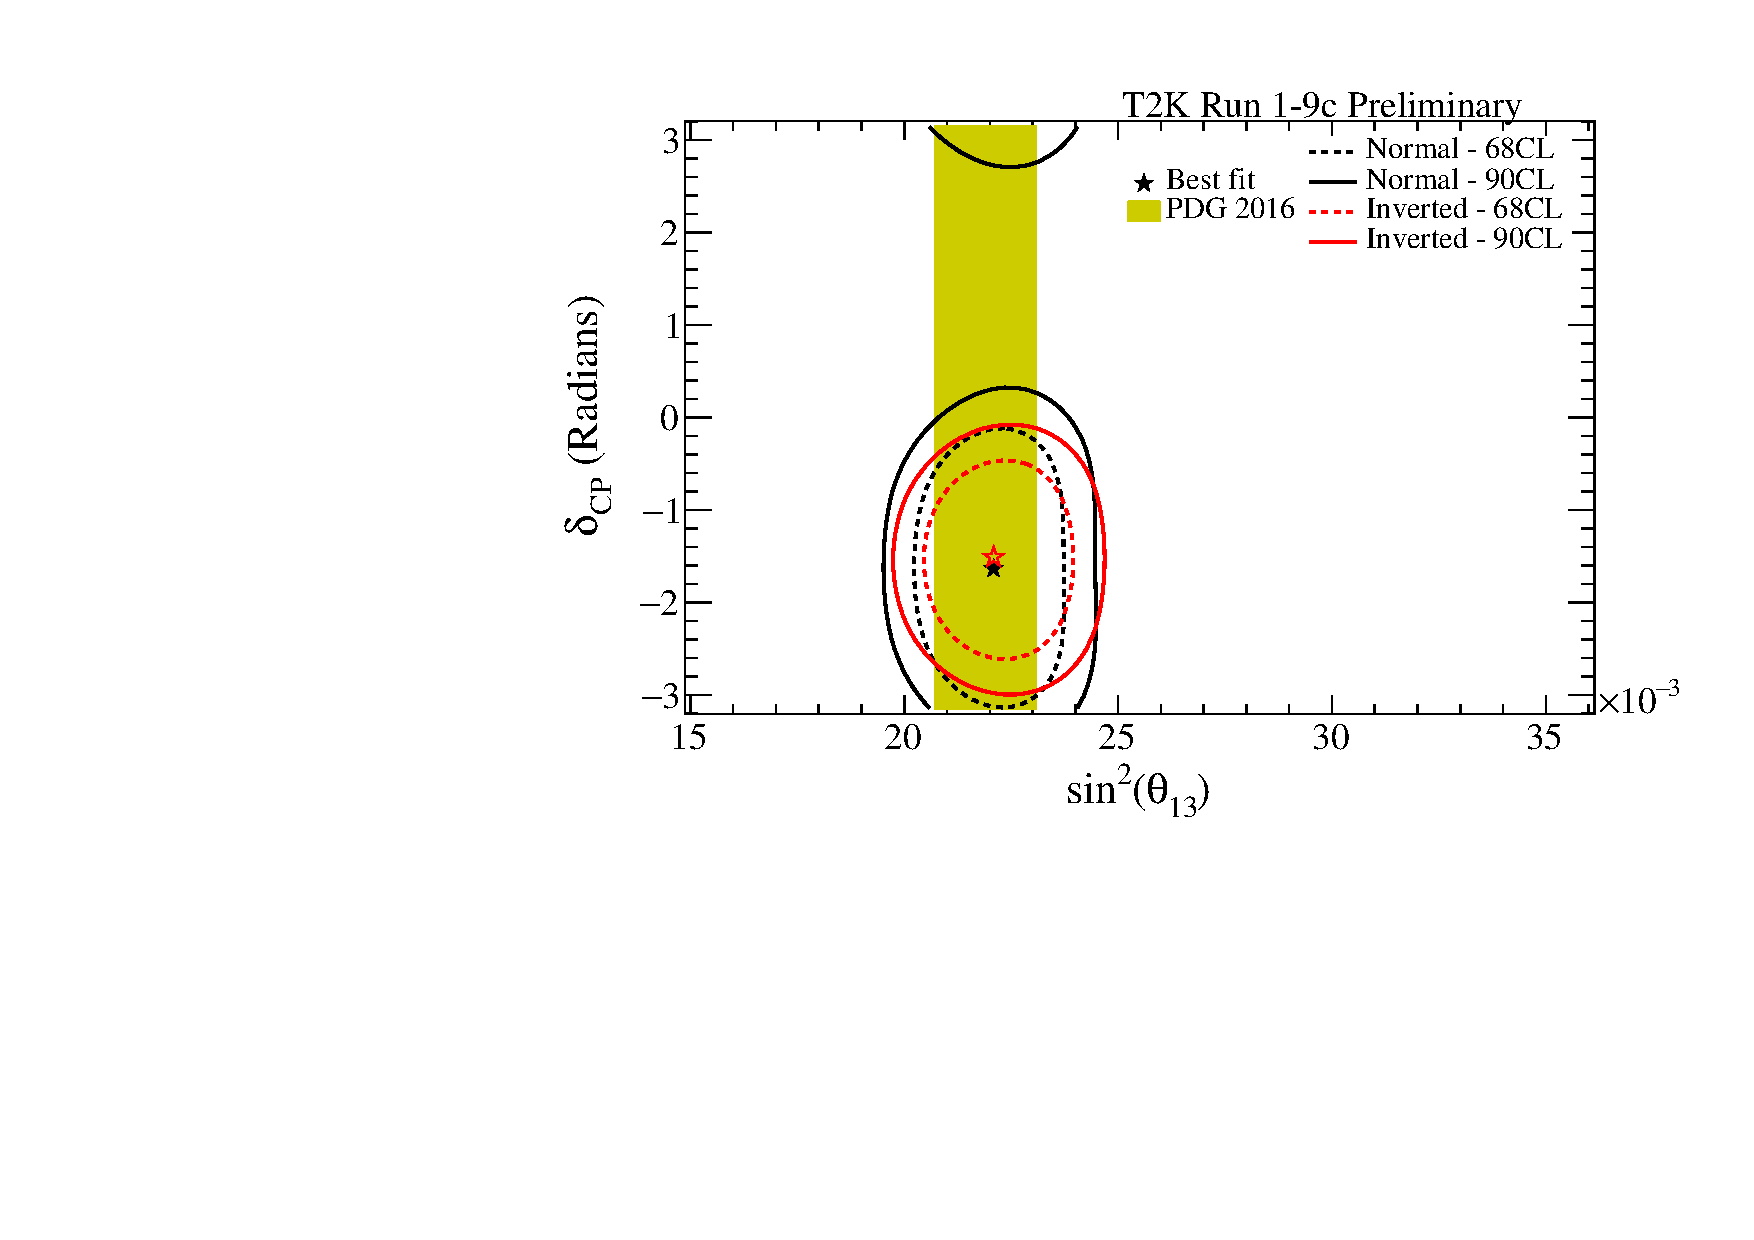
\includegraphics[width=0.9\textwidth]{images/sensitivity/mixing13_deltacp_AsimovA_reactor_global}
		\caption{Asimov A \appearance with reactor constraint}
	\end{subfigure}
	\begin{subfigure}[b]{0.49\textwidth}
		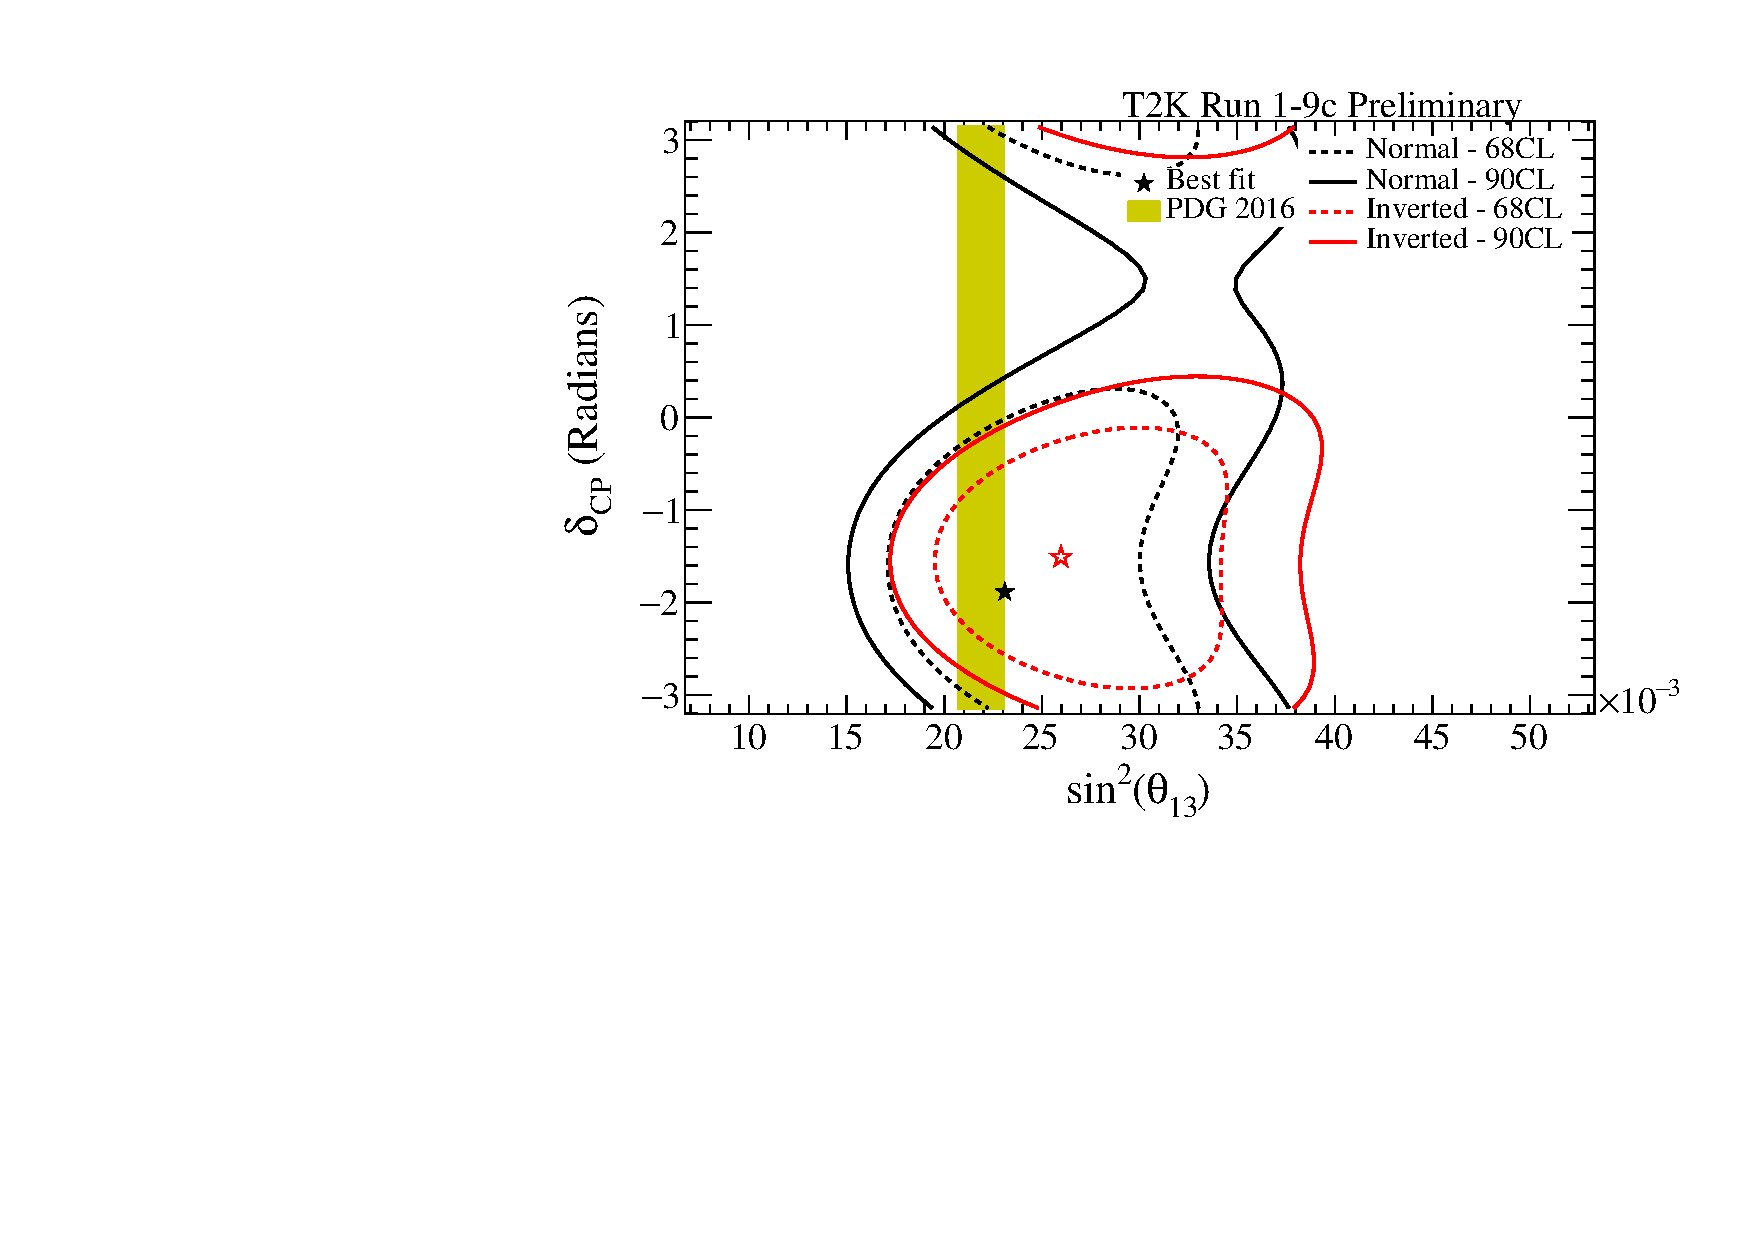
\includegraphics[width=0.9\textwidth]{images/sensitivity/mixing13_deltacp_AsimovA_t2k_global}
		\caption{Asimov A \appearance T2K only}
	\end{subfigure}
	\begin{subfigure}[b]{0.49\textwidth}
		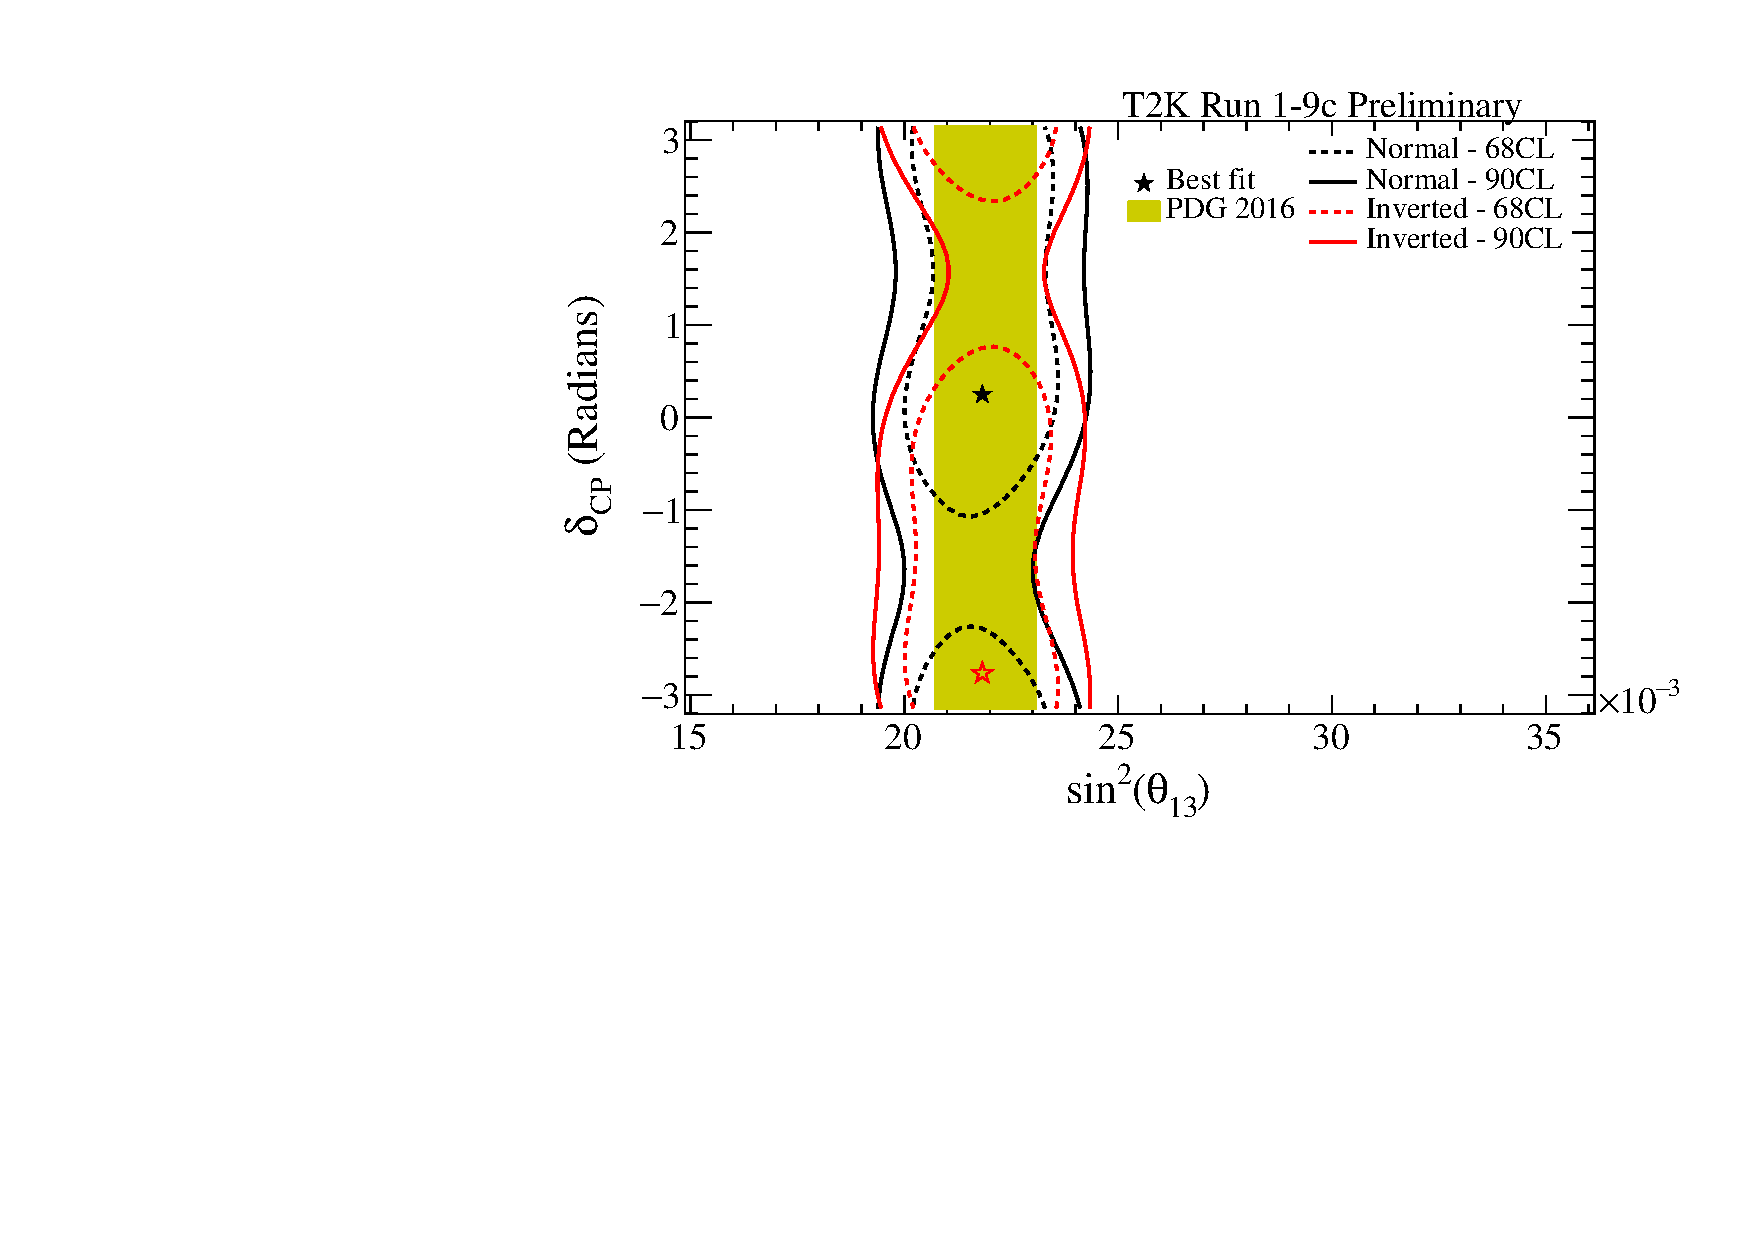
\includegraphics[width=0.9\textwidth]{images/sensitivity/mixing13_deltacp_AsimovB_reactor_global}
		\caption{Asimov B \appearance with reactor constraint}
	\end{subfigure}
	\begin{subfigure}[b]{0.49\textwidth}
		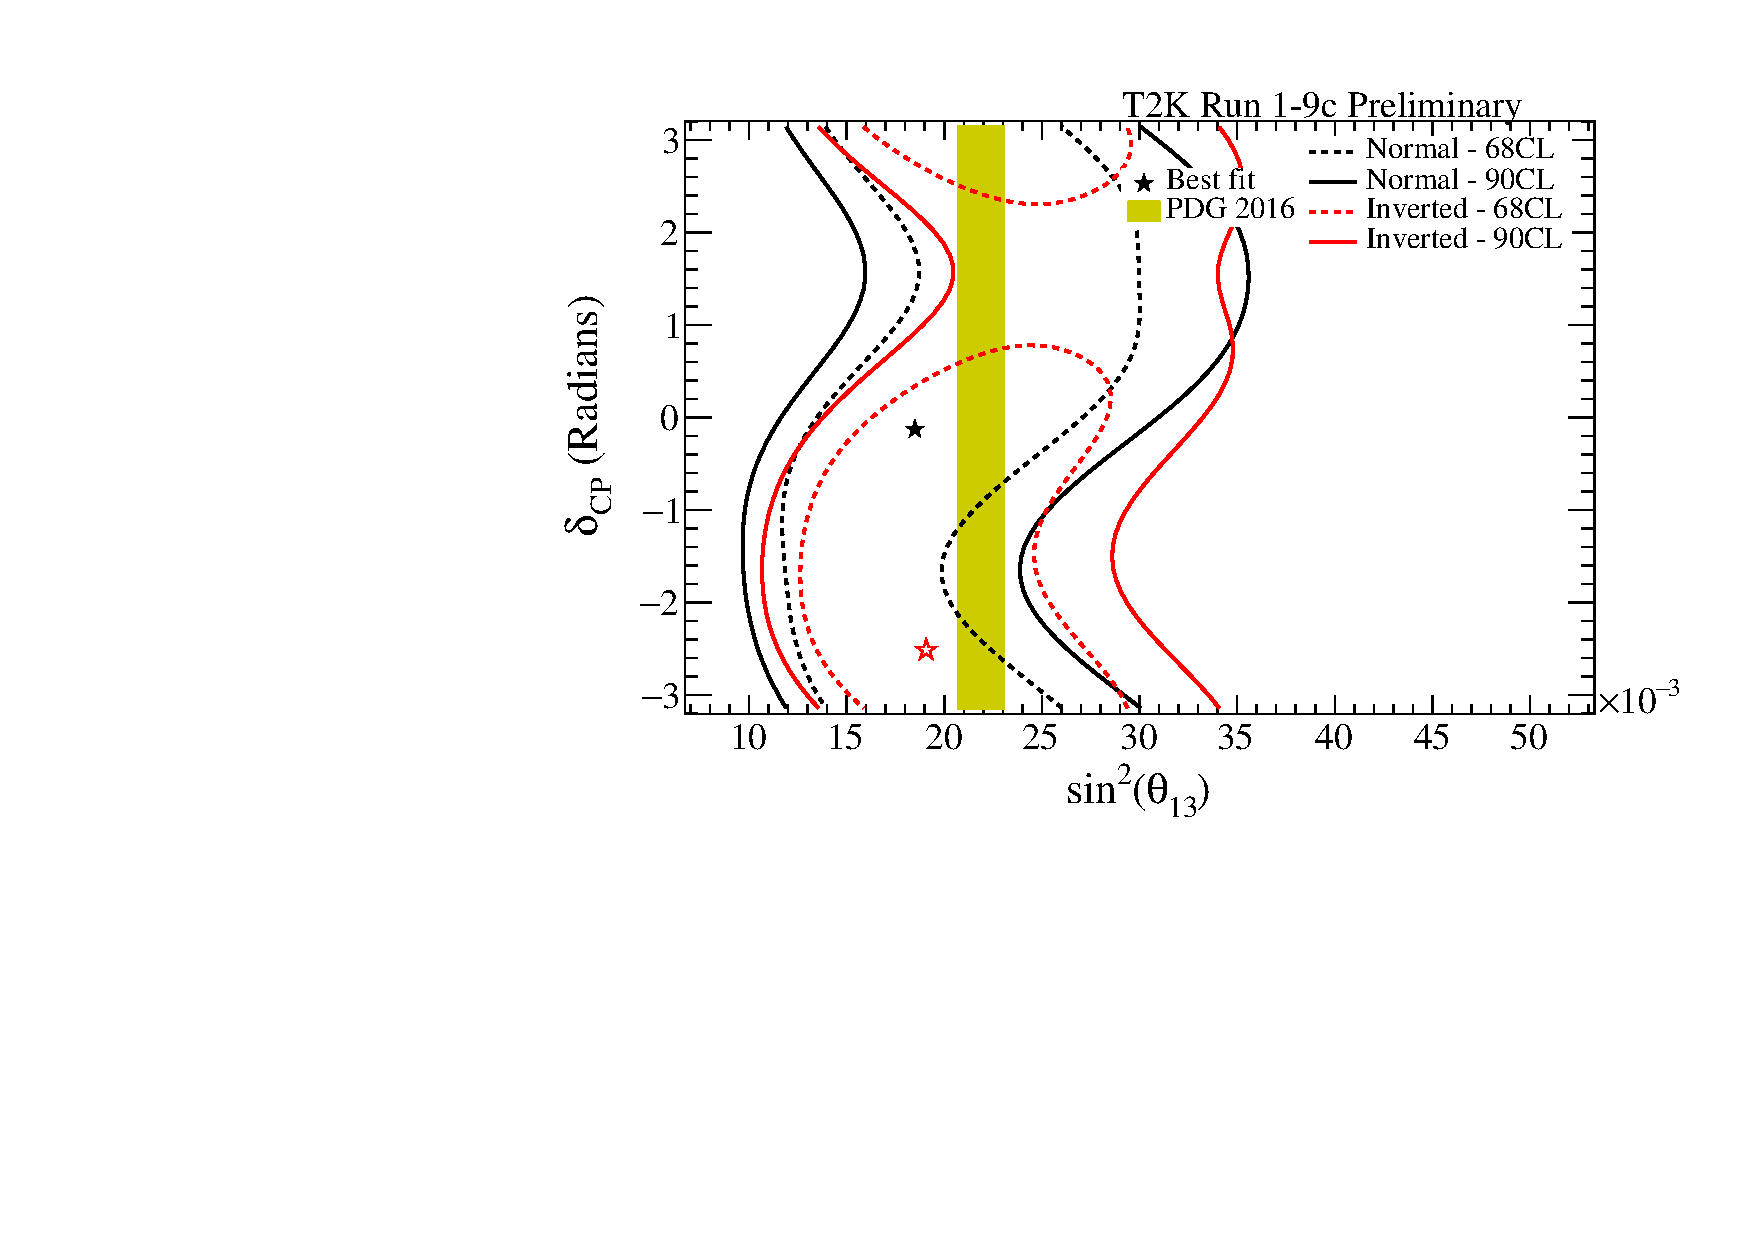
\includegraphics[width=0.9\textwidth]{images/sensitivity/mixing13_deltacp_AsimovB_t2k_global}
		\caption{Asimov B \appearance T2K only}
	\end{subfigure}
	\caption {
		Contours at 68\% and 90\% CL for \appearance with and without reactor constraint for Asimov data sets A and B. Normal and inverted hierarchy contours are independent. All 5 samples were used to produce these fits.
	}
	\label{fig:ssqth13_vs_dcp_sensitivity}
\end{figure*}
\clearpage
\subsubsection{Results for \disappearance}

The sensitivity to \disappearance with reactor constraint and T2K only is shown for the Asimov data sets A and B in fig.~\ref{fig:ssqth23_vs_dmsq23_sensitivity}.

\begin{figure*}[htb]
	\center
	\begin{subfigure}[b]{0.49\textwidth}
		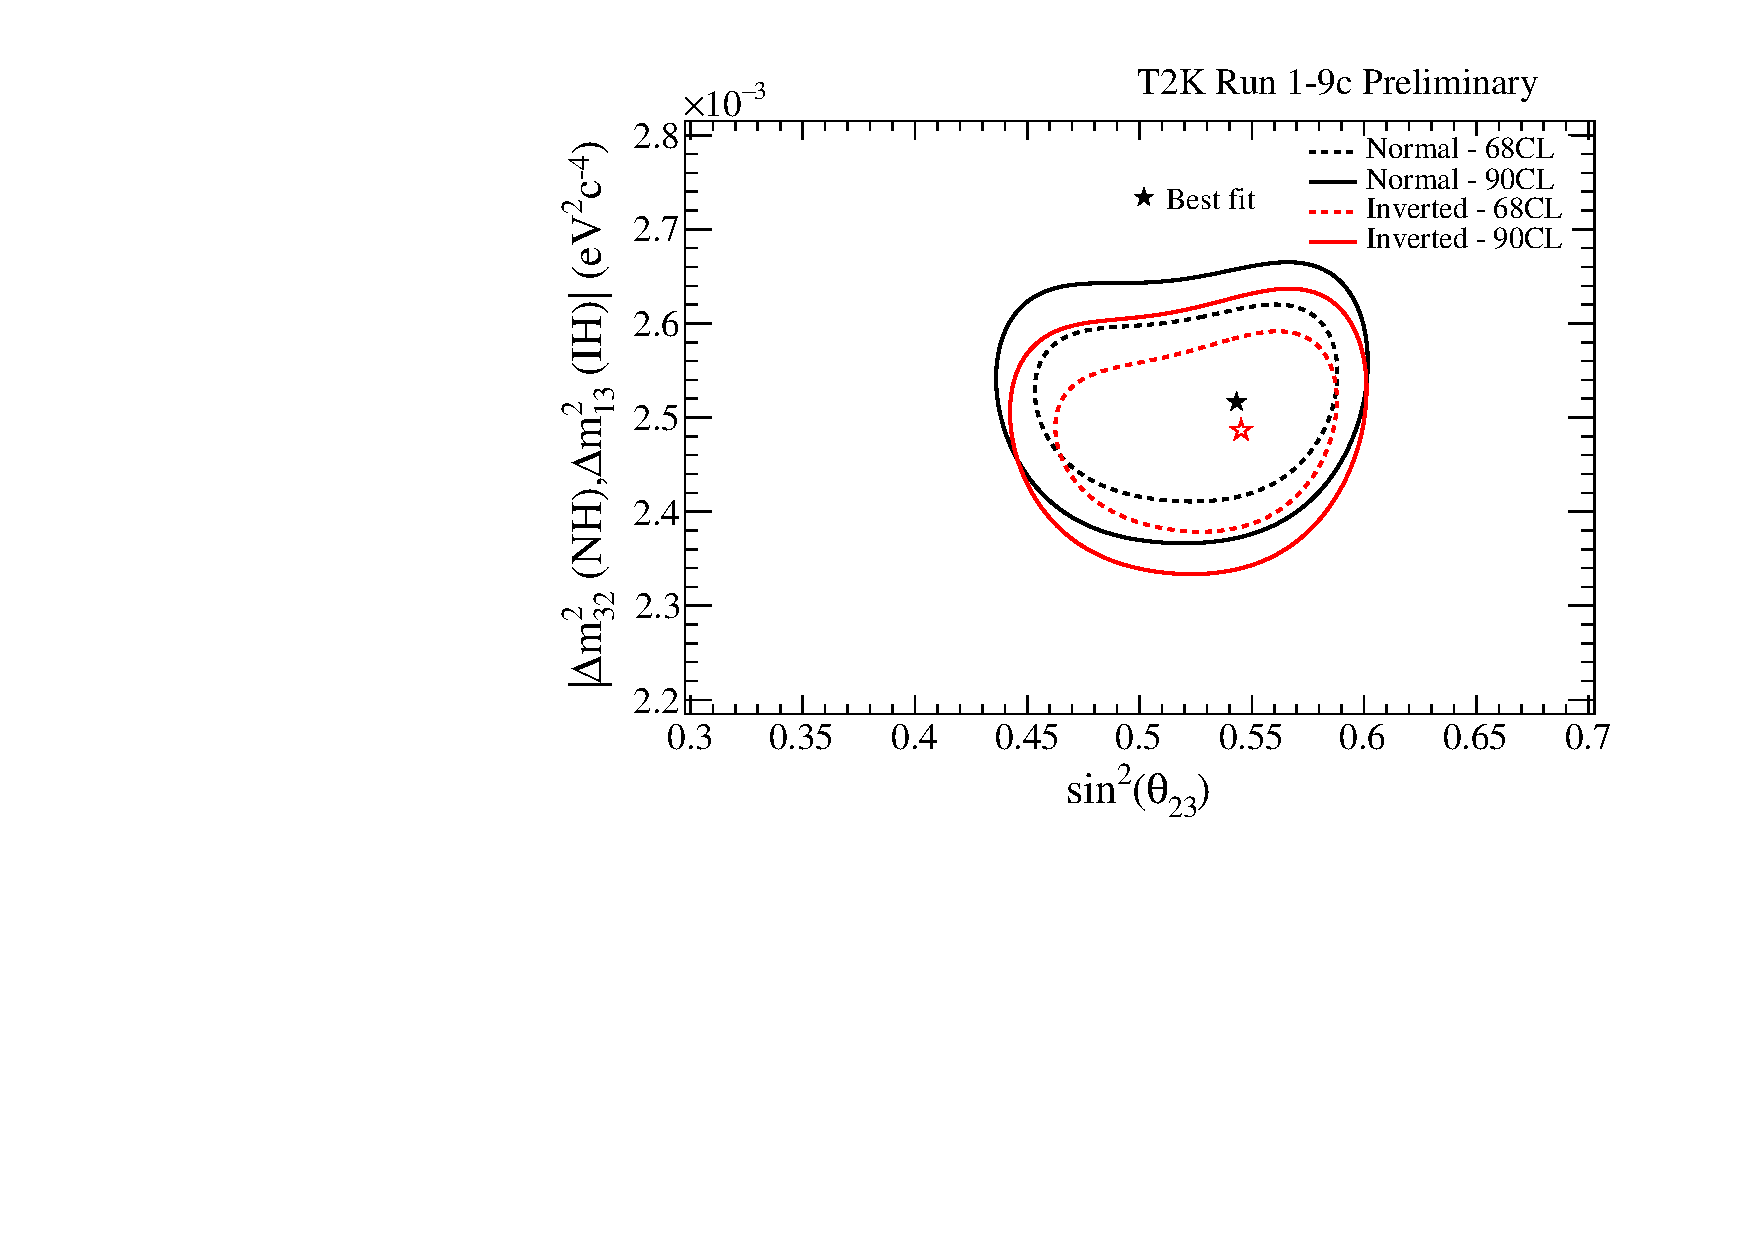
\includegraphics[width=0.9\textwidth]{images/sensitivity/mixing23_dmsq23_AsimovA_reactor_global}
		\caption{Asimov A \disappearance with reactor constraint}
	\end{subfigure}
	\begin{subfigure}[b]{0.49\textwidth}
		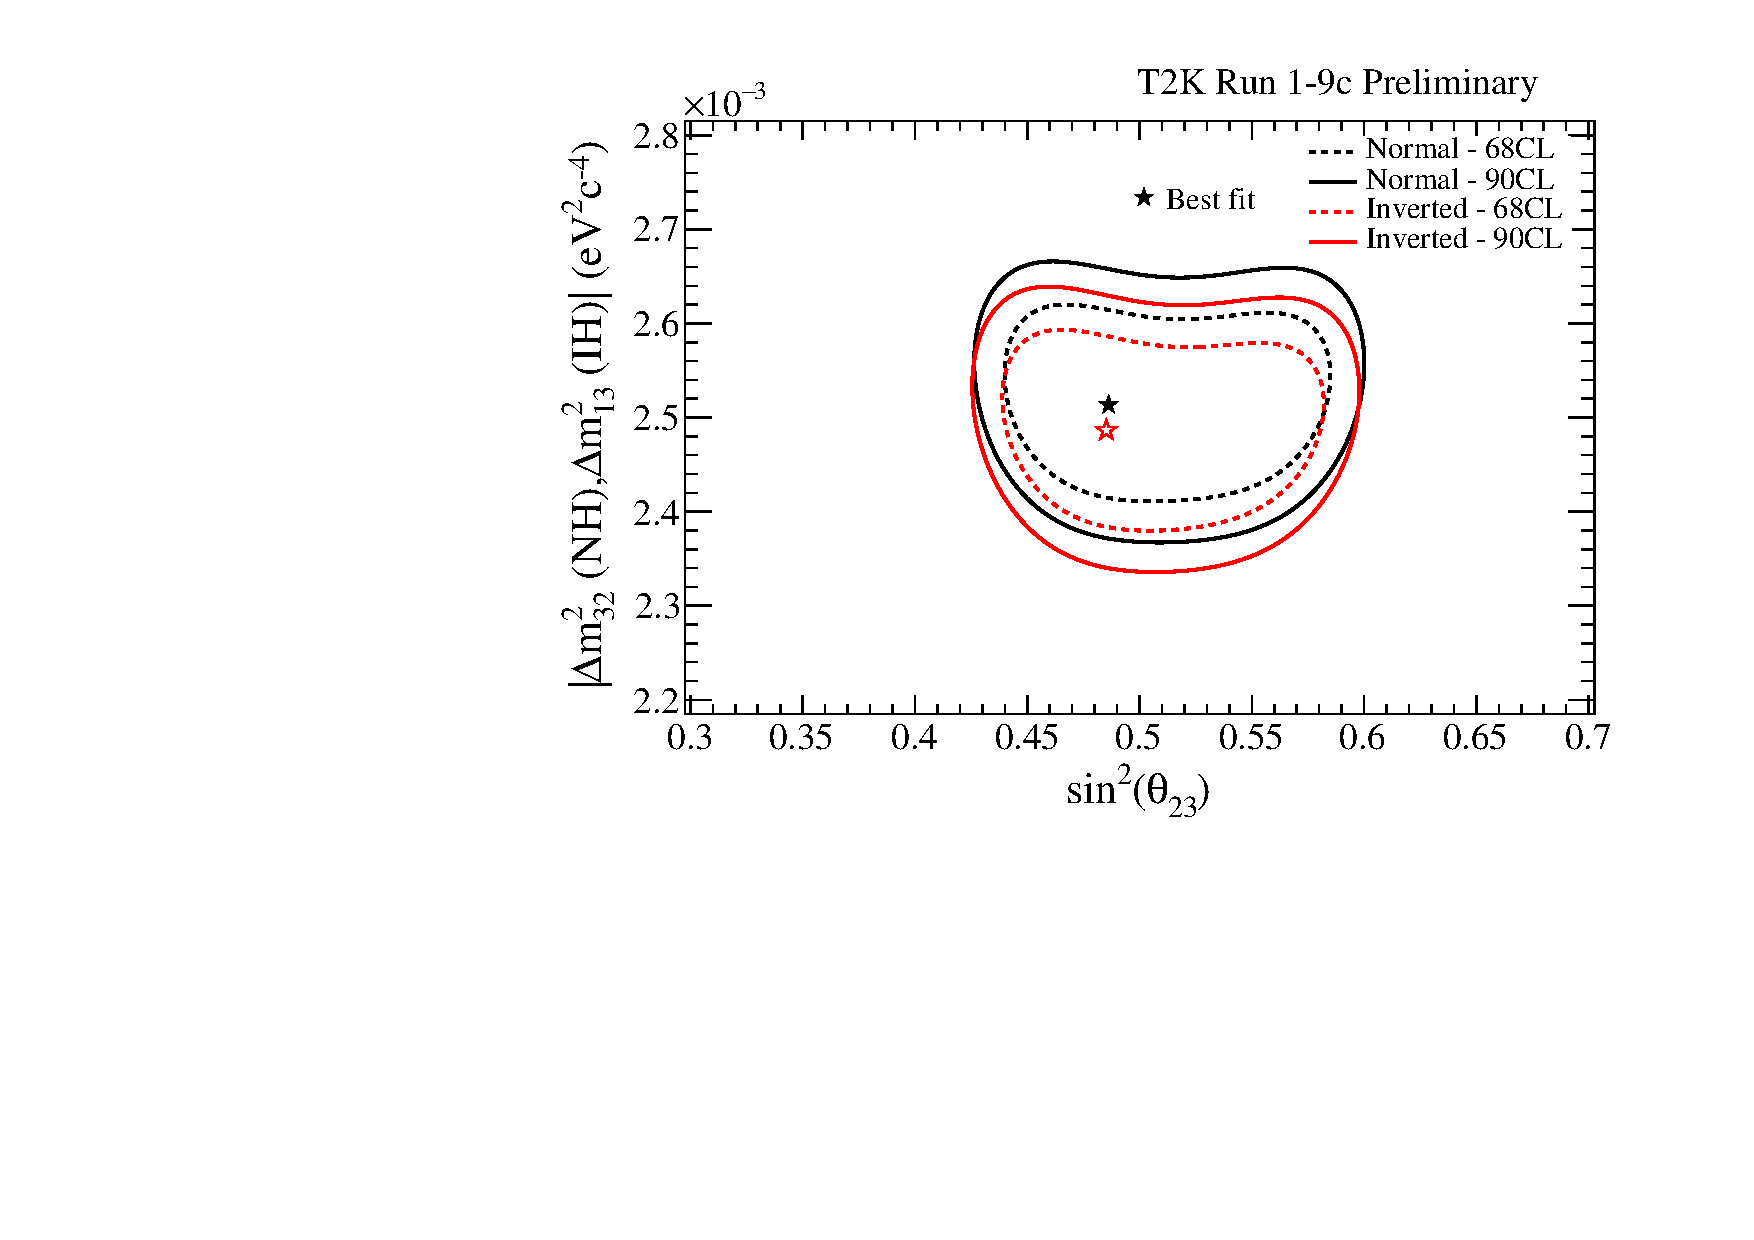
\includegraphics[width=0.9\textwidth]{images/sensitivity/mixing23_dmsq23_AsimovA_t2k_global}
		\caption{Asimov A \disappearance T2K only}
	\end{subfigure}
	\begin{subfigure}[b]{0.49\textwidth}
		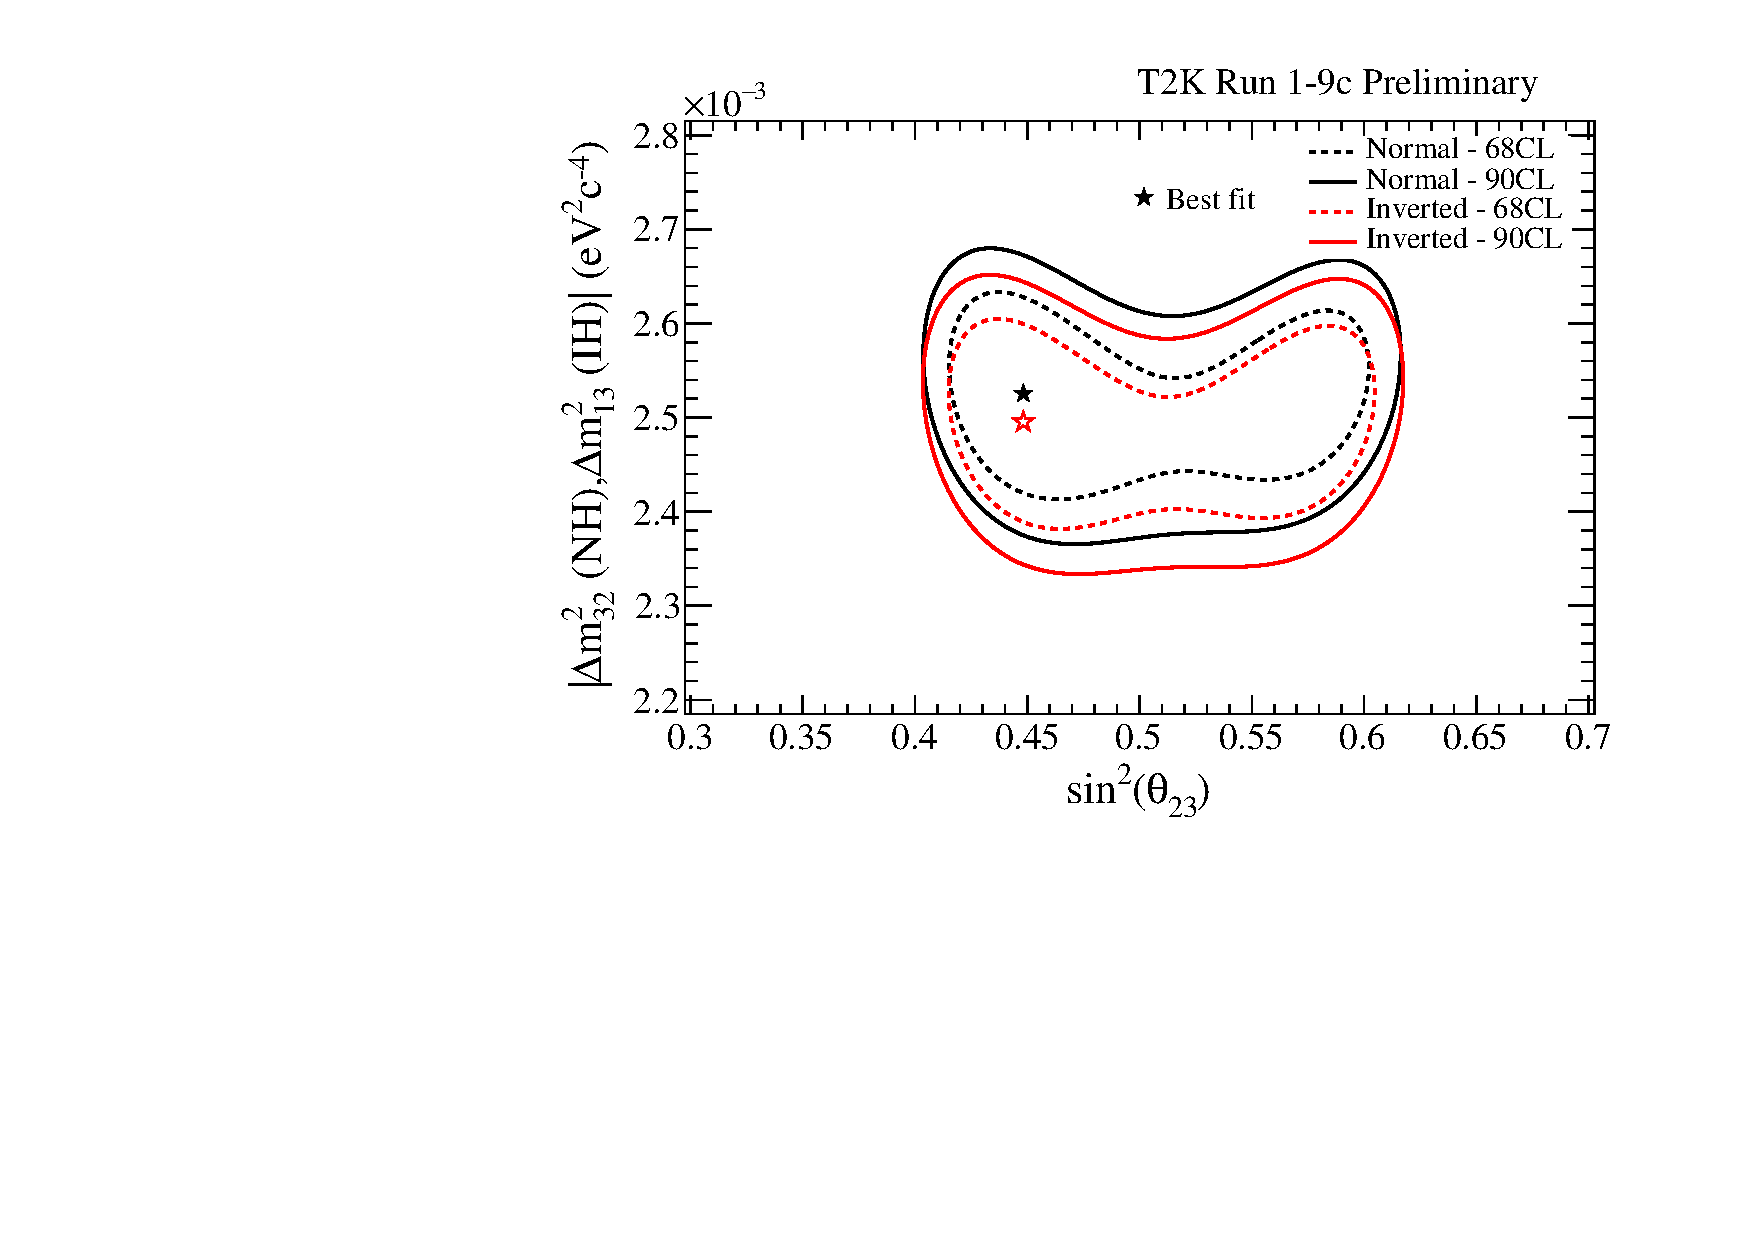
\includegraphics[width=0.9\textwidth]{images/sensitivity/mixing23_dmsq23_AsimovB_reactor_global}
		\caption{Asimov B \disappearance with reactor constraint}
	\end{subfigure}
	\begin{subfigure}[b]{0.49\textwidth}
		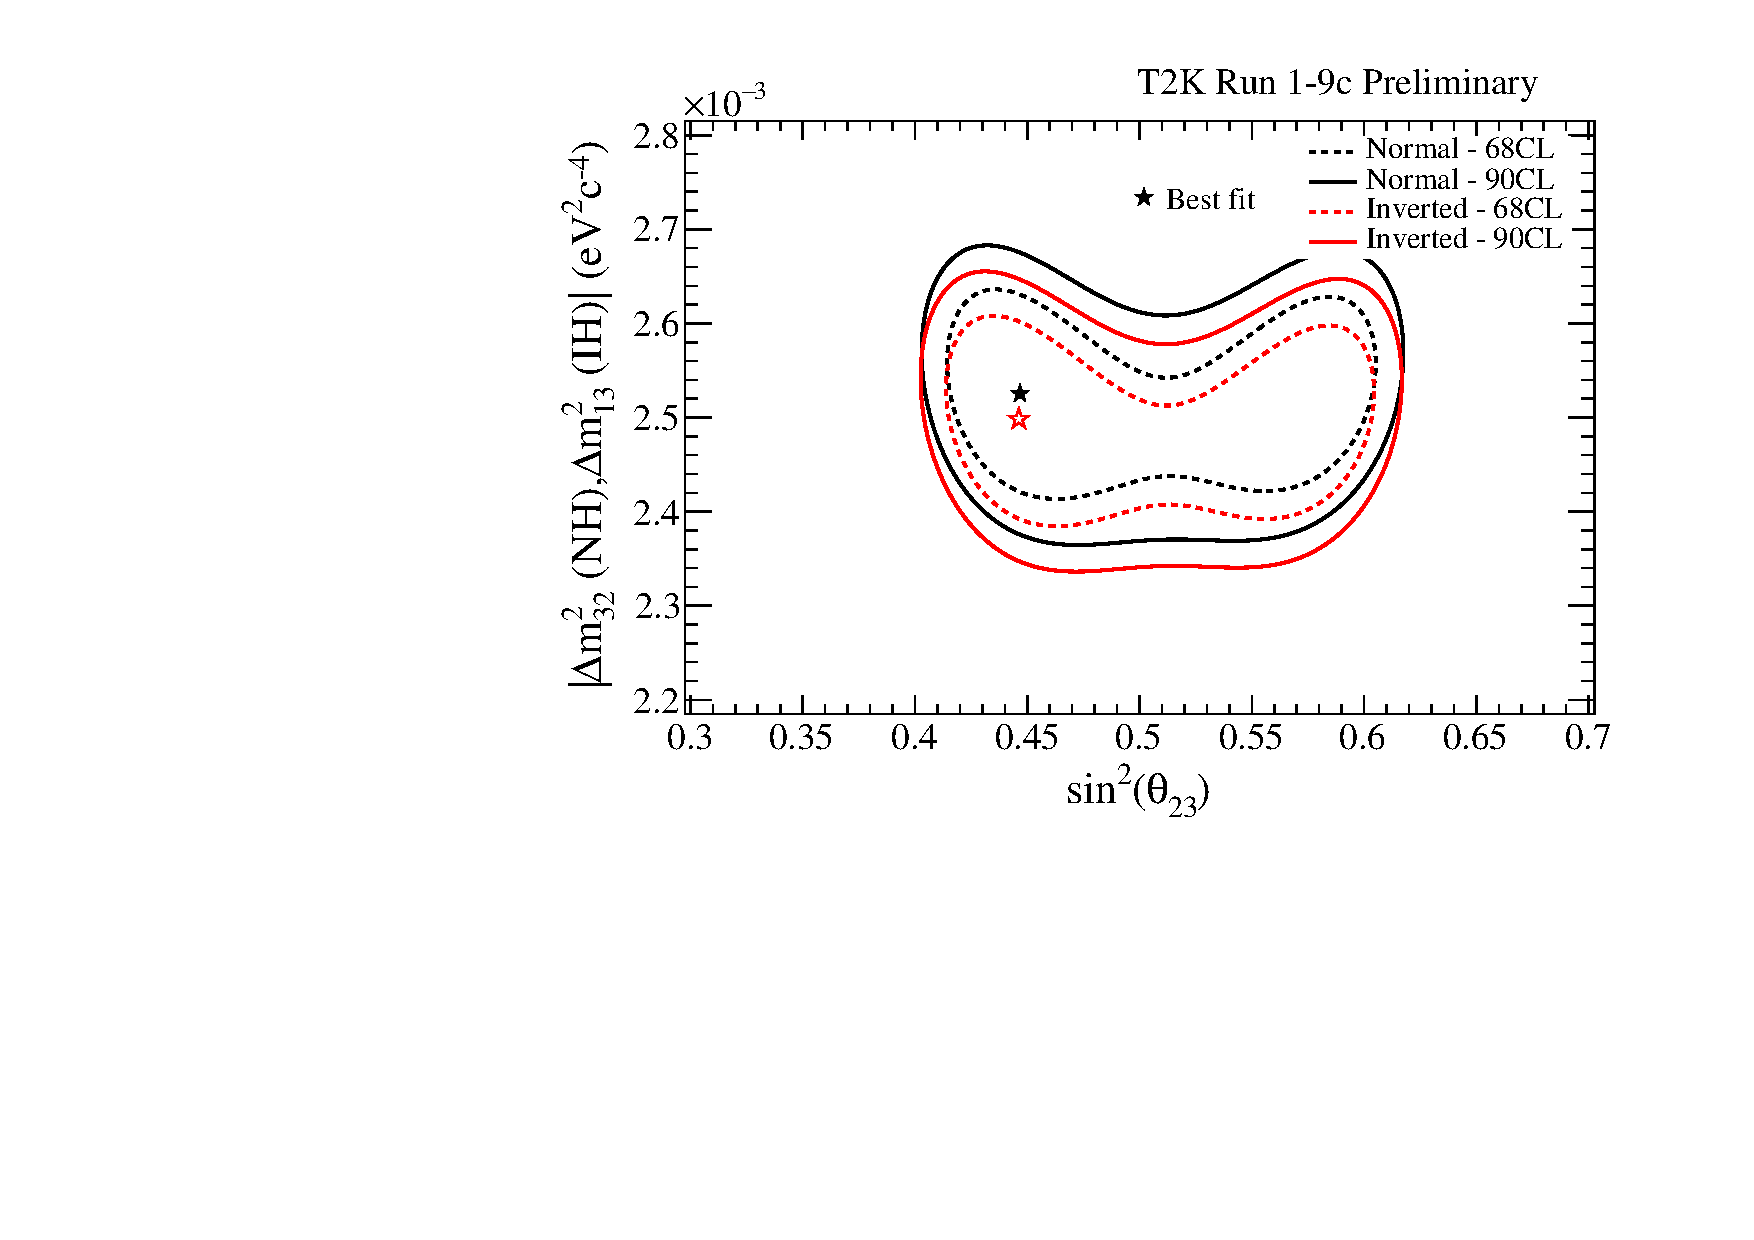
\includegraphics[width=0.9\textwidth]{images/sensitivity/mixing23_dmsq23_AsimovB_t2k_global}
		\caption{Asimov B \disappearance T2K only}
	\end{subfigure}
	\caption {
		Contours at 68\% and 90\% CL for \disappearance with and without reactor constraint for Asimov data sets A and B. Normal and inverted hierarchy contours are independent. All 5 samples were used to produce these fits.
	}
	\label{fig:ssqth23_vs_dmsq23_sensitivity}
\end{figure*}
\clearpage
\subsubsection{Results for \deltacp}

The sensitivity to \deltacp with reactor constraint and T2K only is shown for the Asimov data sets A and B in fig.~\ref{fig:dcp_sensitivity}.

\begin{figure*}[htb]
	\center
	\begin{subfigure}[b]{0.49\textwidth}
		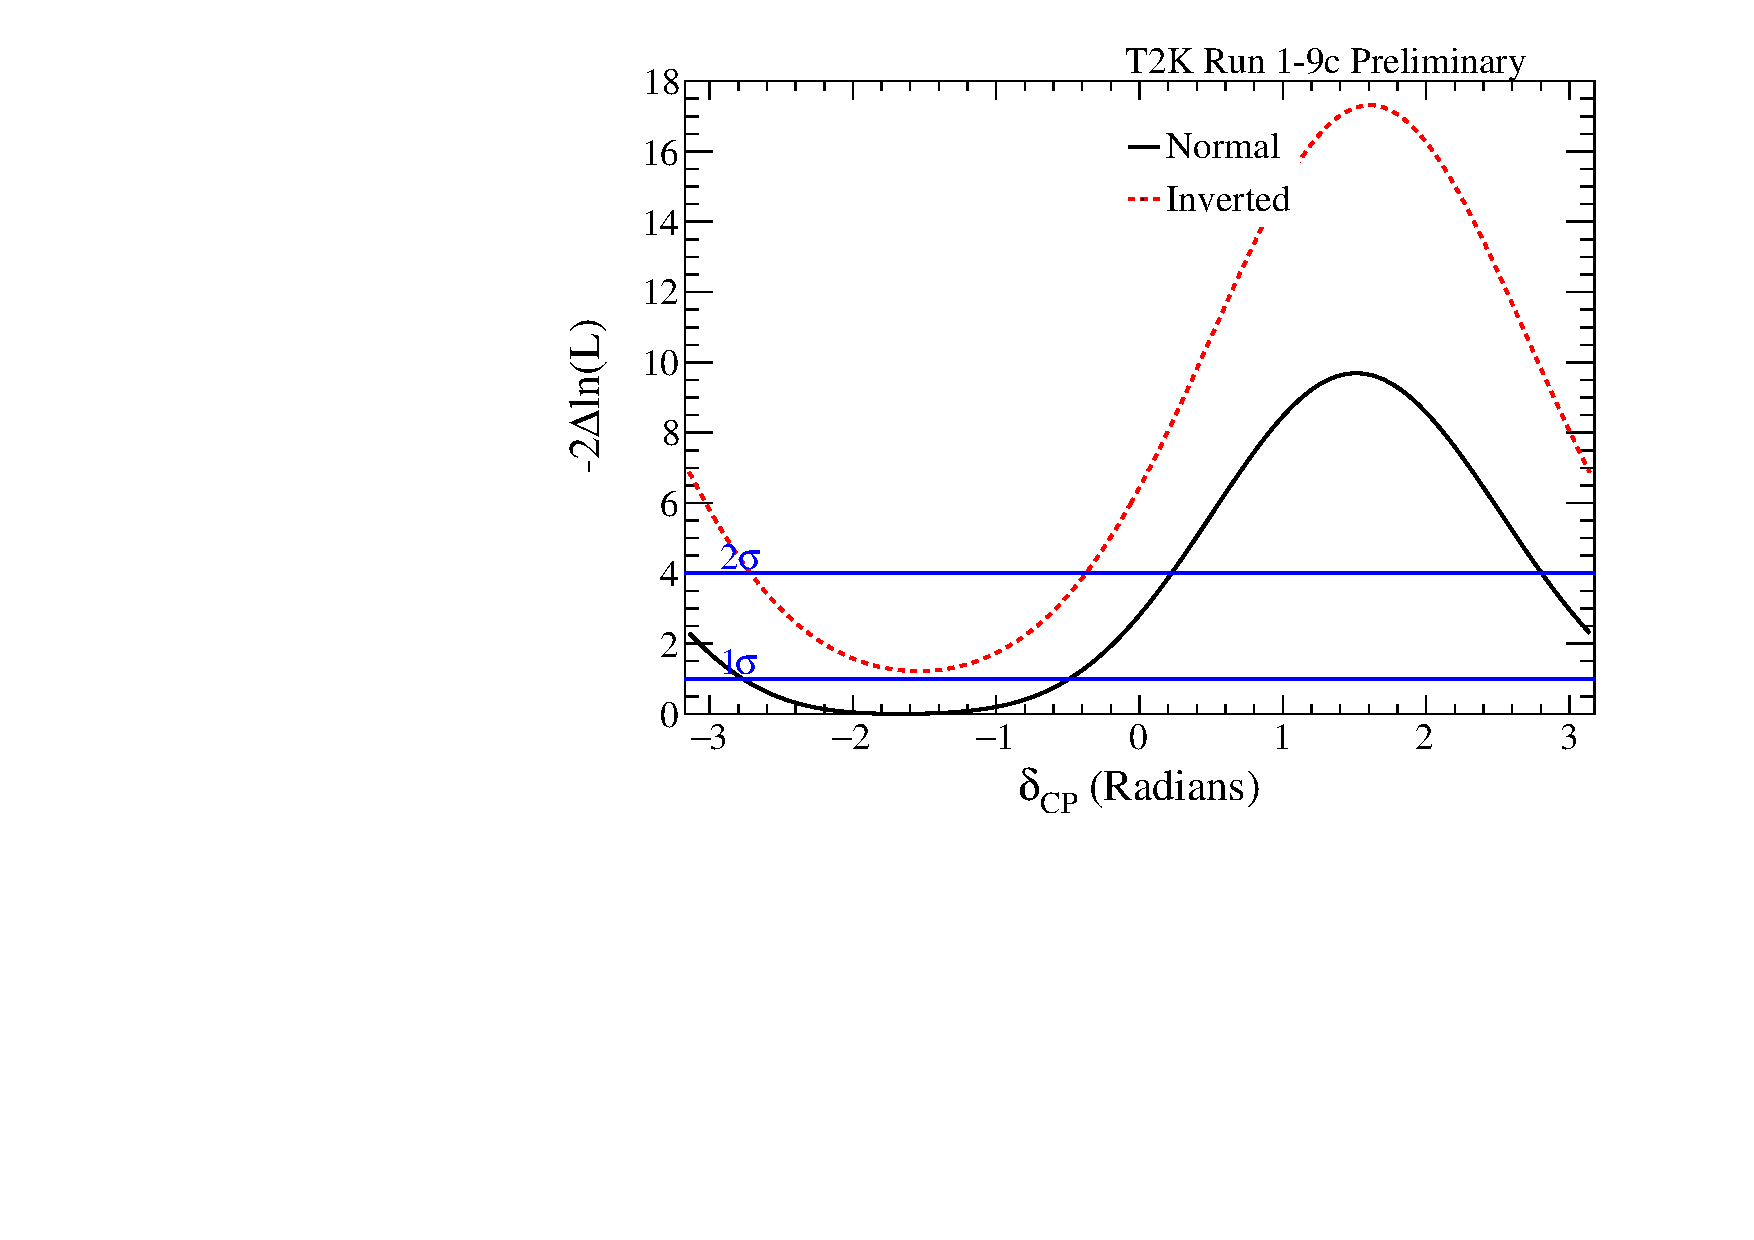
\includegraphics[width=0.9\textwidth]{images/sensitivity/deltacp_AsimovA_reactor_global}
		\caption{Asimov A \deltacp with reactor constraint}
	\end{subfigure}
	\begin{subfigure}[b]{0.49\textwidth}
		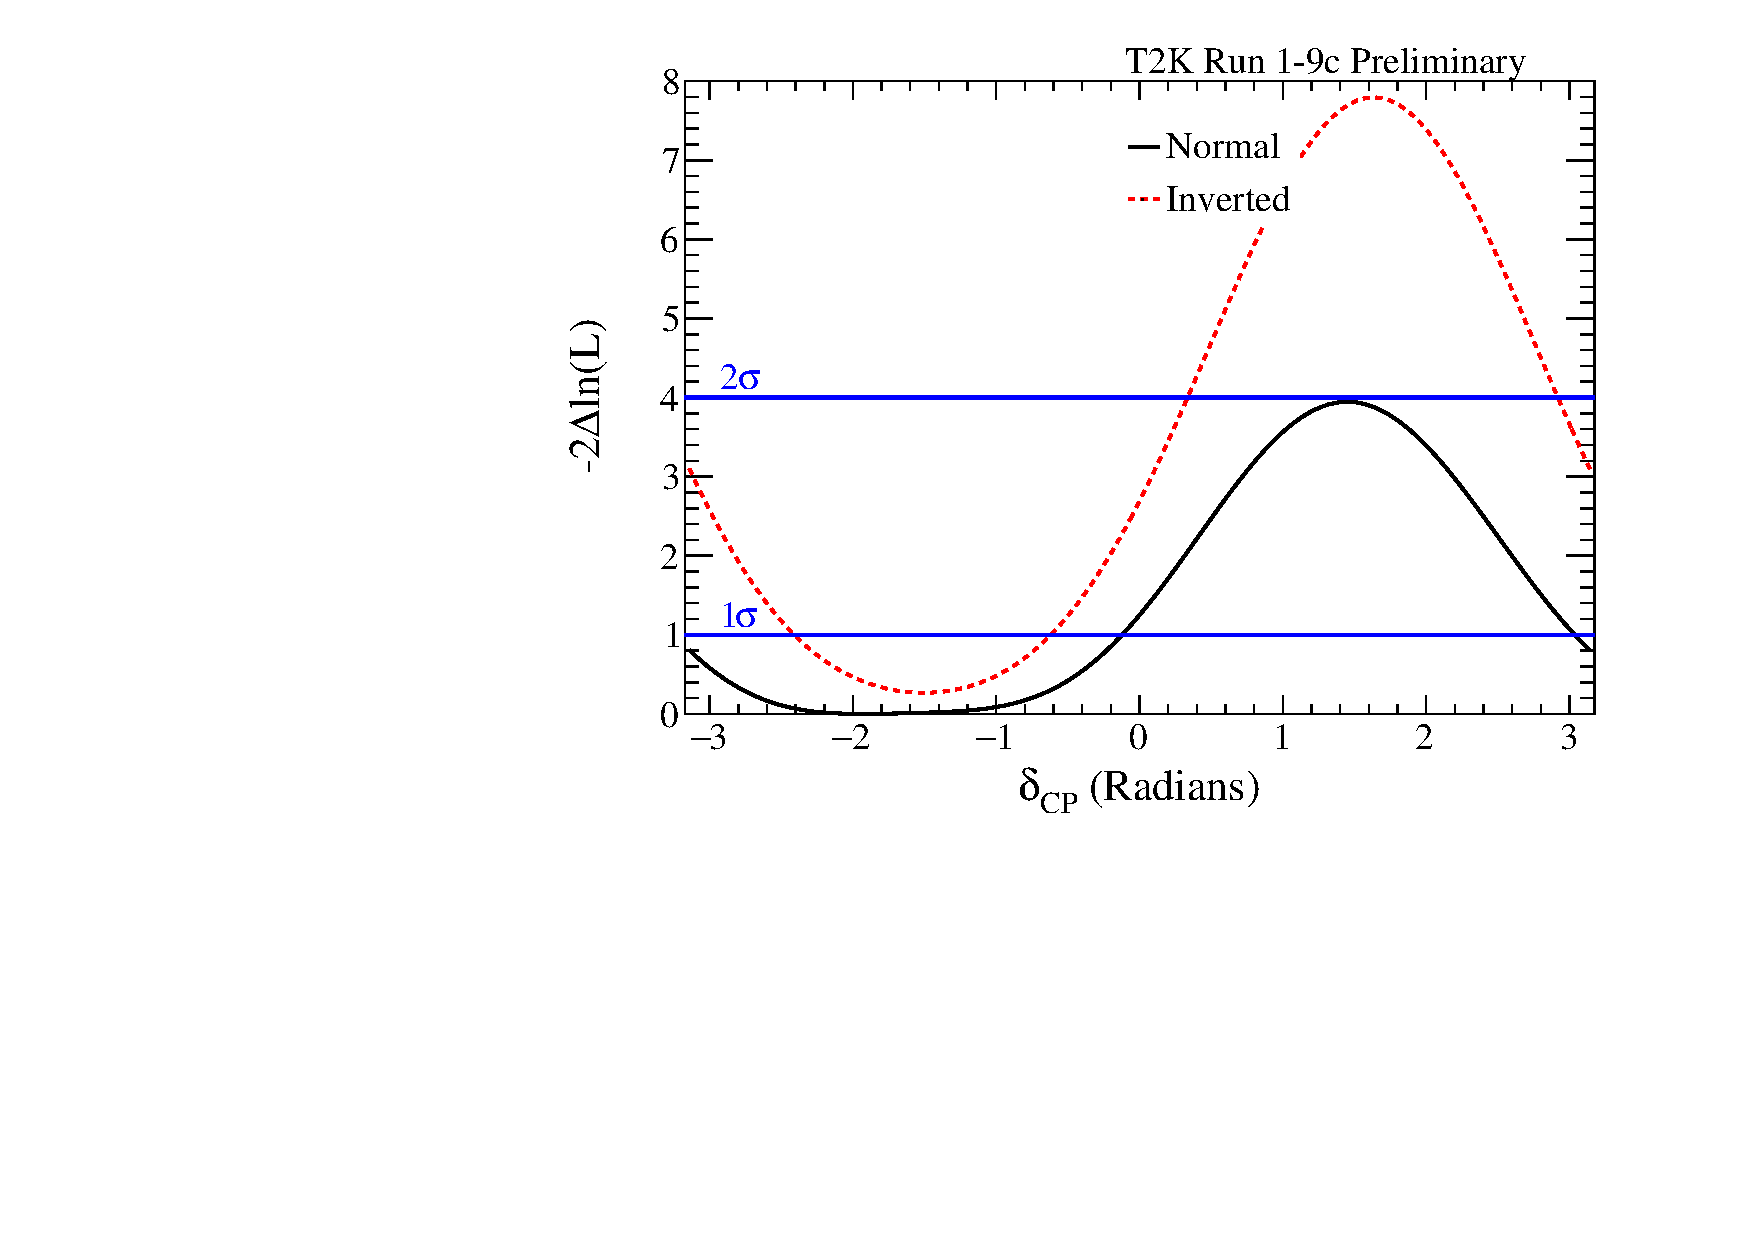
\includegraphics[width=0.9\textwidth]{images/sensitivity/deltacp_AsimovA_t2k_global}
		\caption{Asimov A \deltacp T2K only}
	\end{subfigure}
	\begin{subfigure}[b]{0.49\textwidth}
		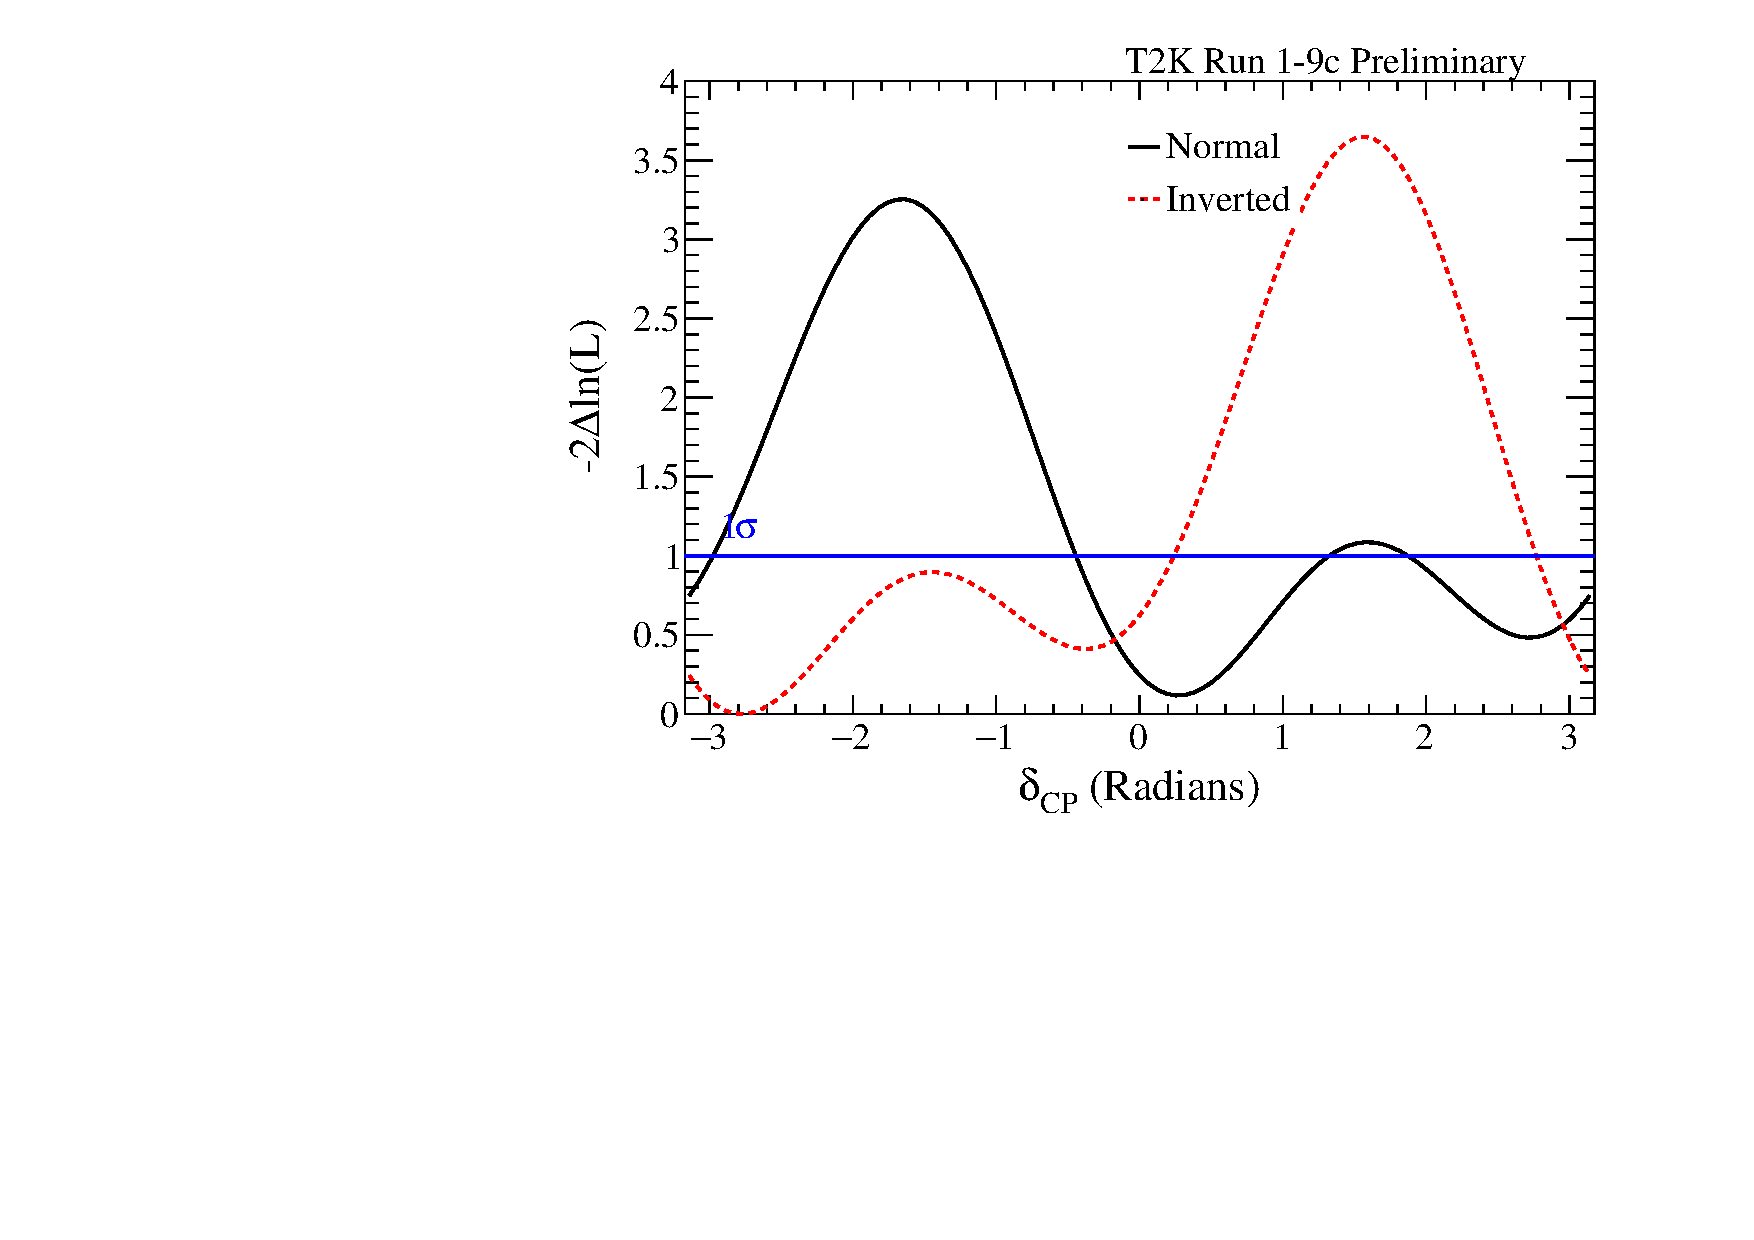
\includegraphics[width=0.9\textwidth]{images/sensitivity/deltacp_AsimovB_reactor_global}
		\caption{Asimov B \deltacp with reactor constraint}
	\end{subfigure}
	\begin{subfigure}[b]{0.49\textwidth}
		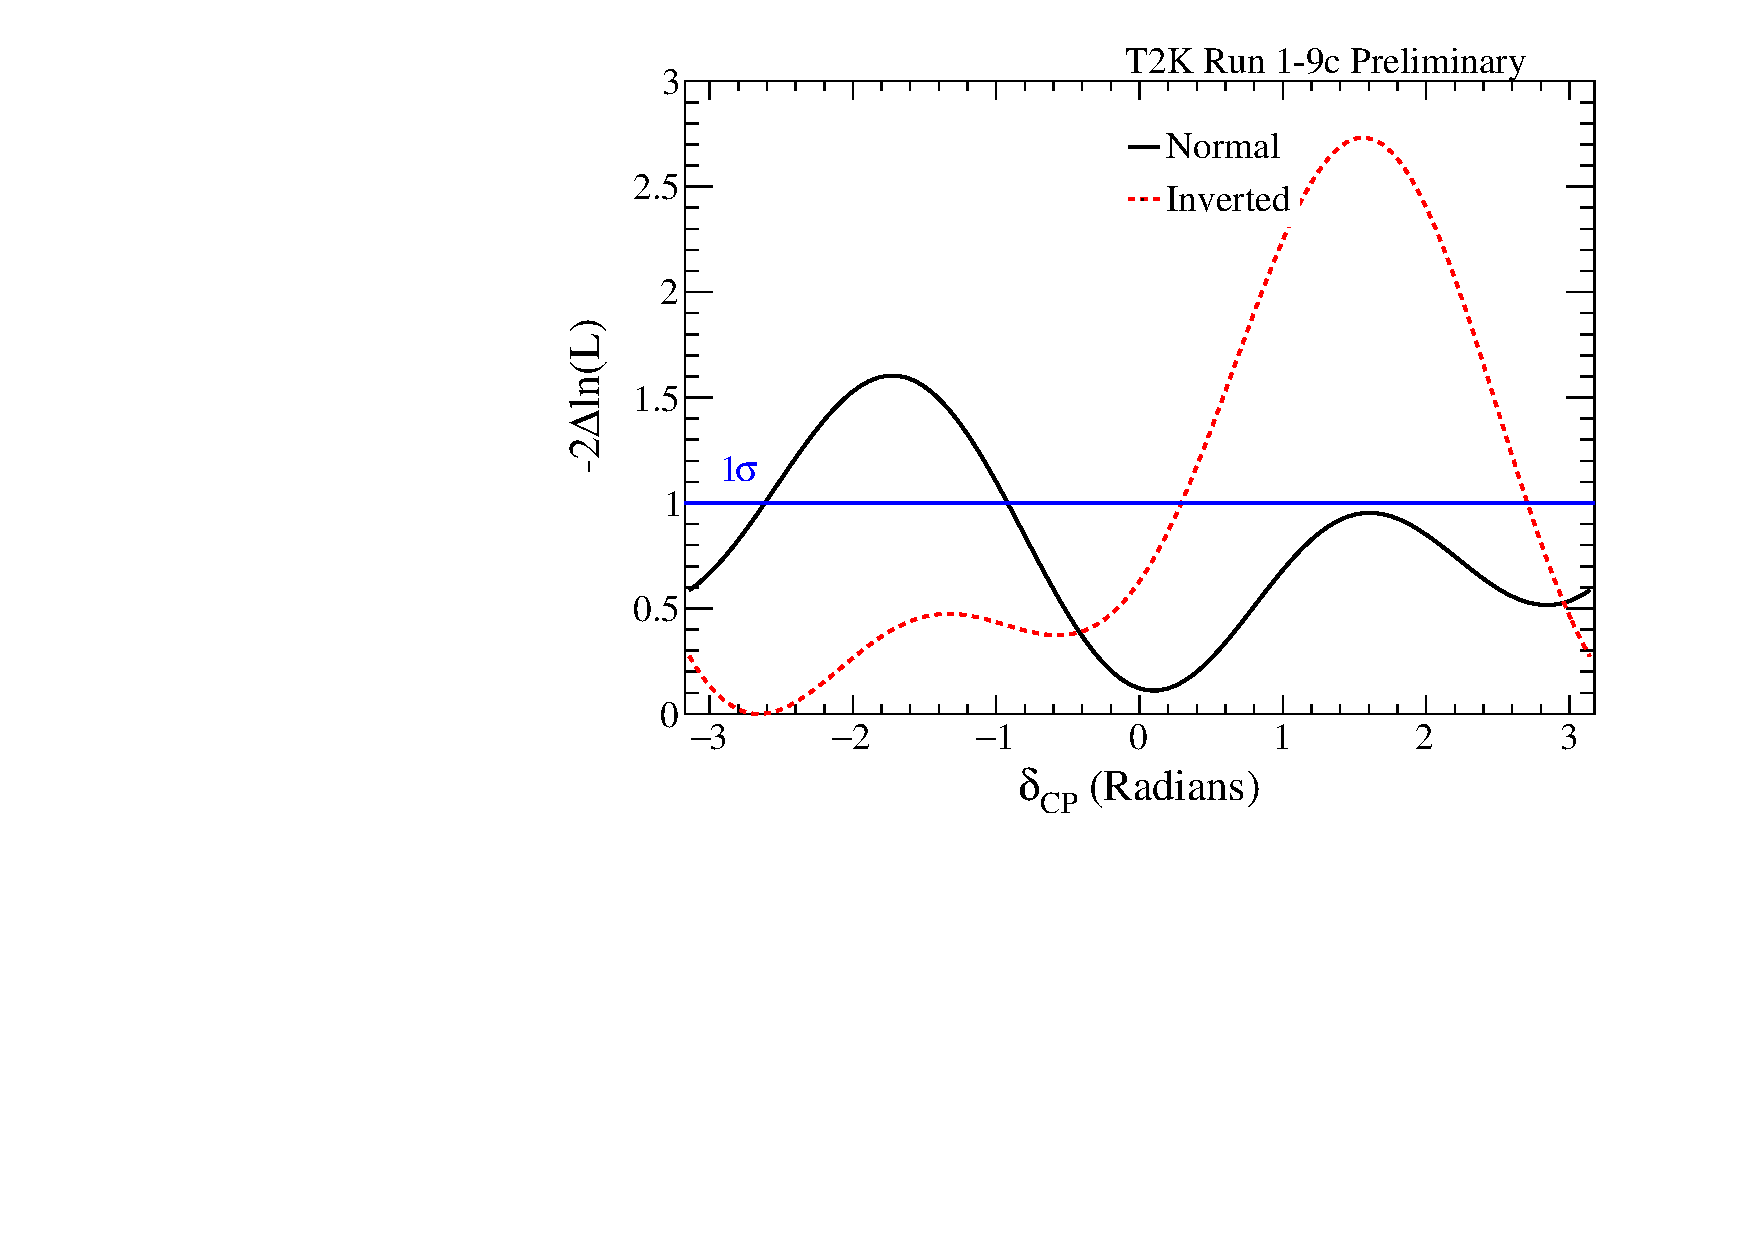
\includegraphics[width=0.9\textwidth]{images/sensitivity/deltacp_AsimovB_t2k_global}
		\caption{Asimov B \deltacp T2K only}
	\end{subfigure}
	\caption {
		The expected $\Delta\chi^2$ distribution as a function of \deltacp with and without reactor constraint for Asimov data sets A and B. The mass hierarchy is minimized, with normal and inverted hierarchy $\Delta\chi^2$ distributions shifted to the same global best-fit $\chi^2$ value, which is taken to be the minimum between normal and inverted hierarchy. All 5 samples were used to produce these fits.
	}
	\label{fig:dcp_sensitivity}
\end{figure*}
\clearpage
\subsubsection{Results for \ssqthonethree}

The sensitivity to \ssqthonethree (without reactor constraint) is shown for the Asimov data sets A and B in fig.~\ref{fig:th13_sensitivity}.

\begin{figure*}[htb]
	\center
	\begin{subfigure}[b]{0.49\textwidth}
		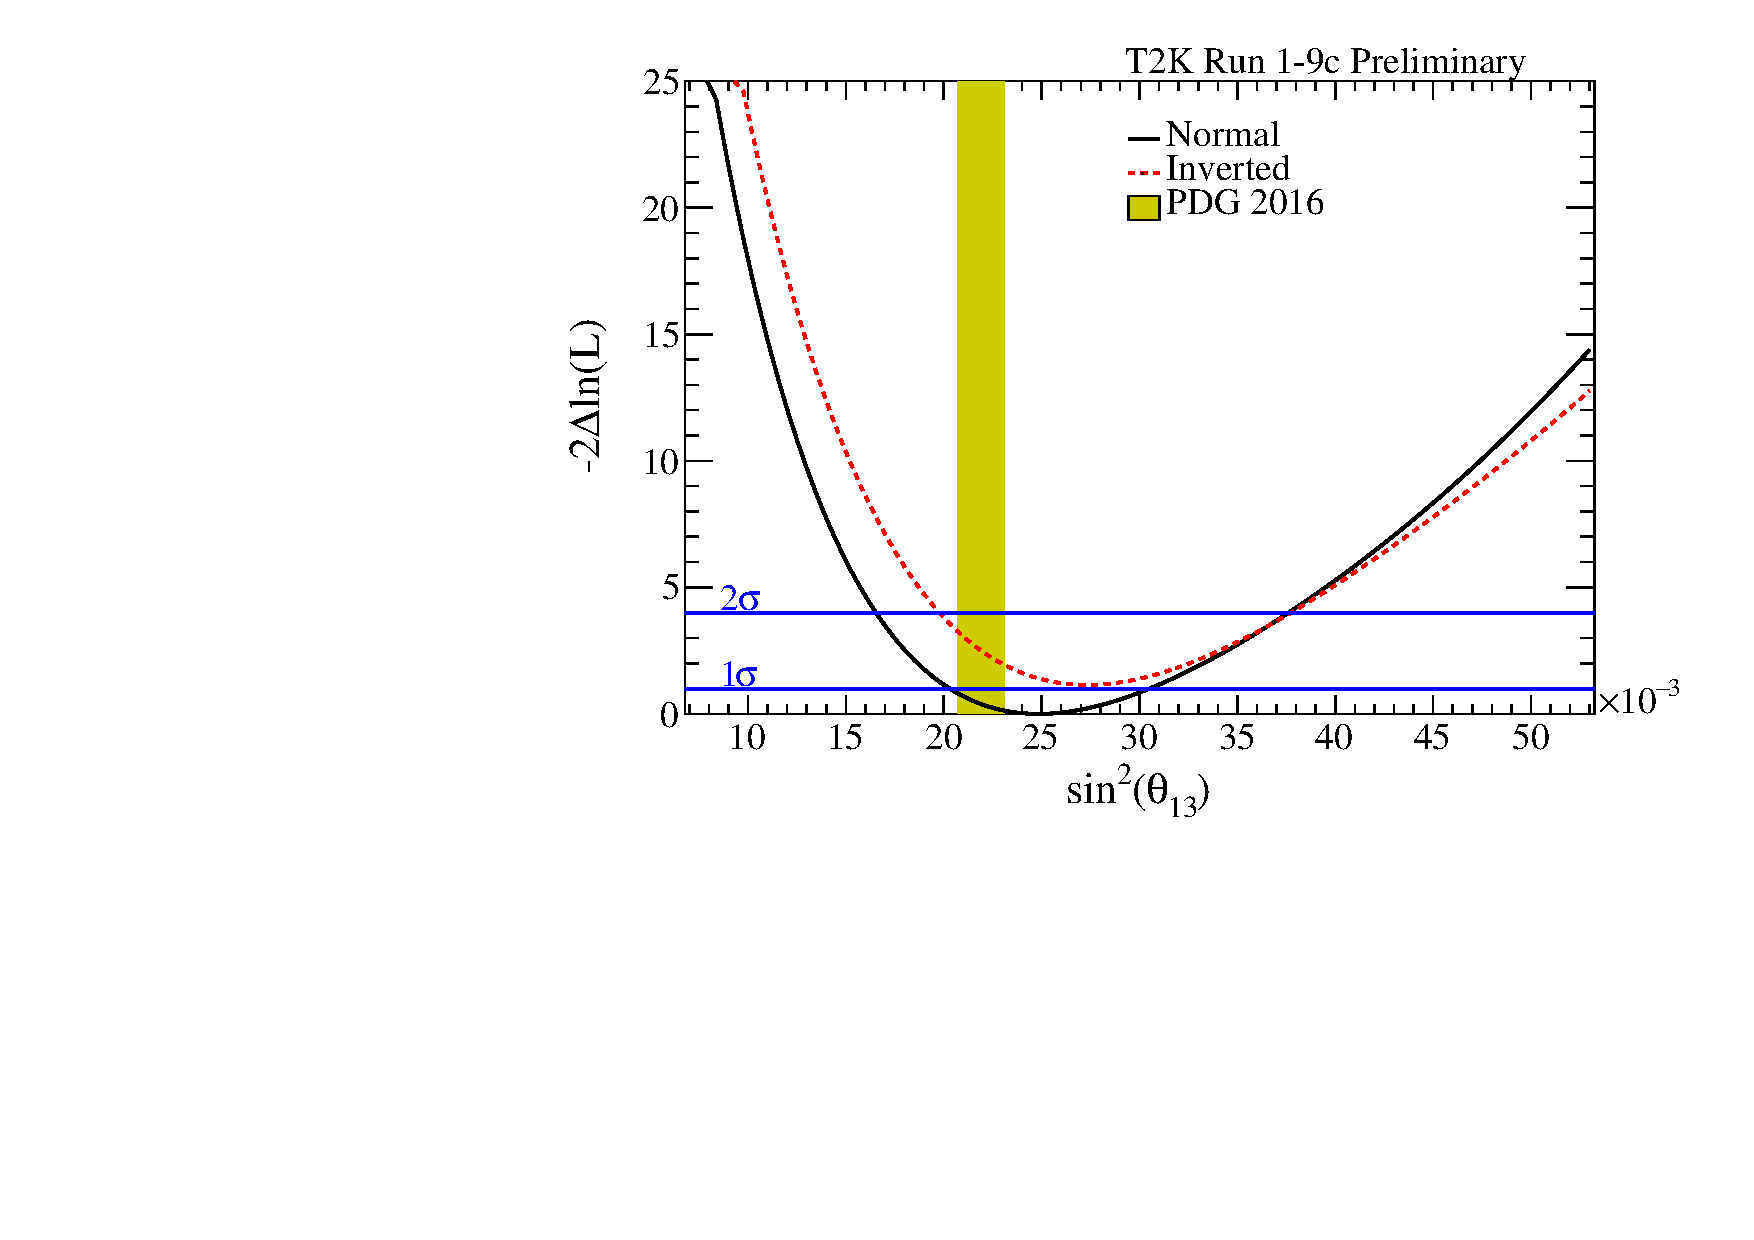
\includegraphics[width=0.9\textwidth]{images/sensitivity/mixing13_AsimovA_t2k_global}
		\caption{Asimov A \ssqthonethree T2K only}
	\end{subfigure}
	\begin{subfigure}[b]{0.49\textwidth}
		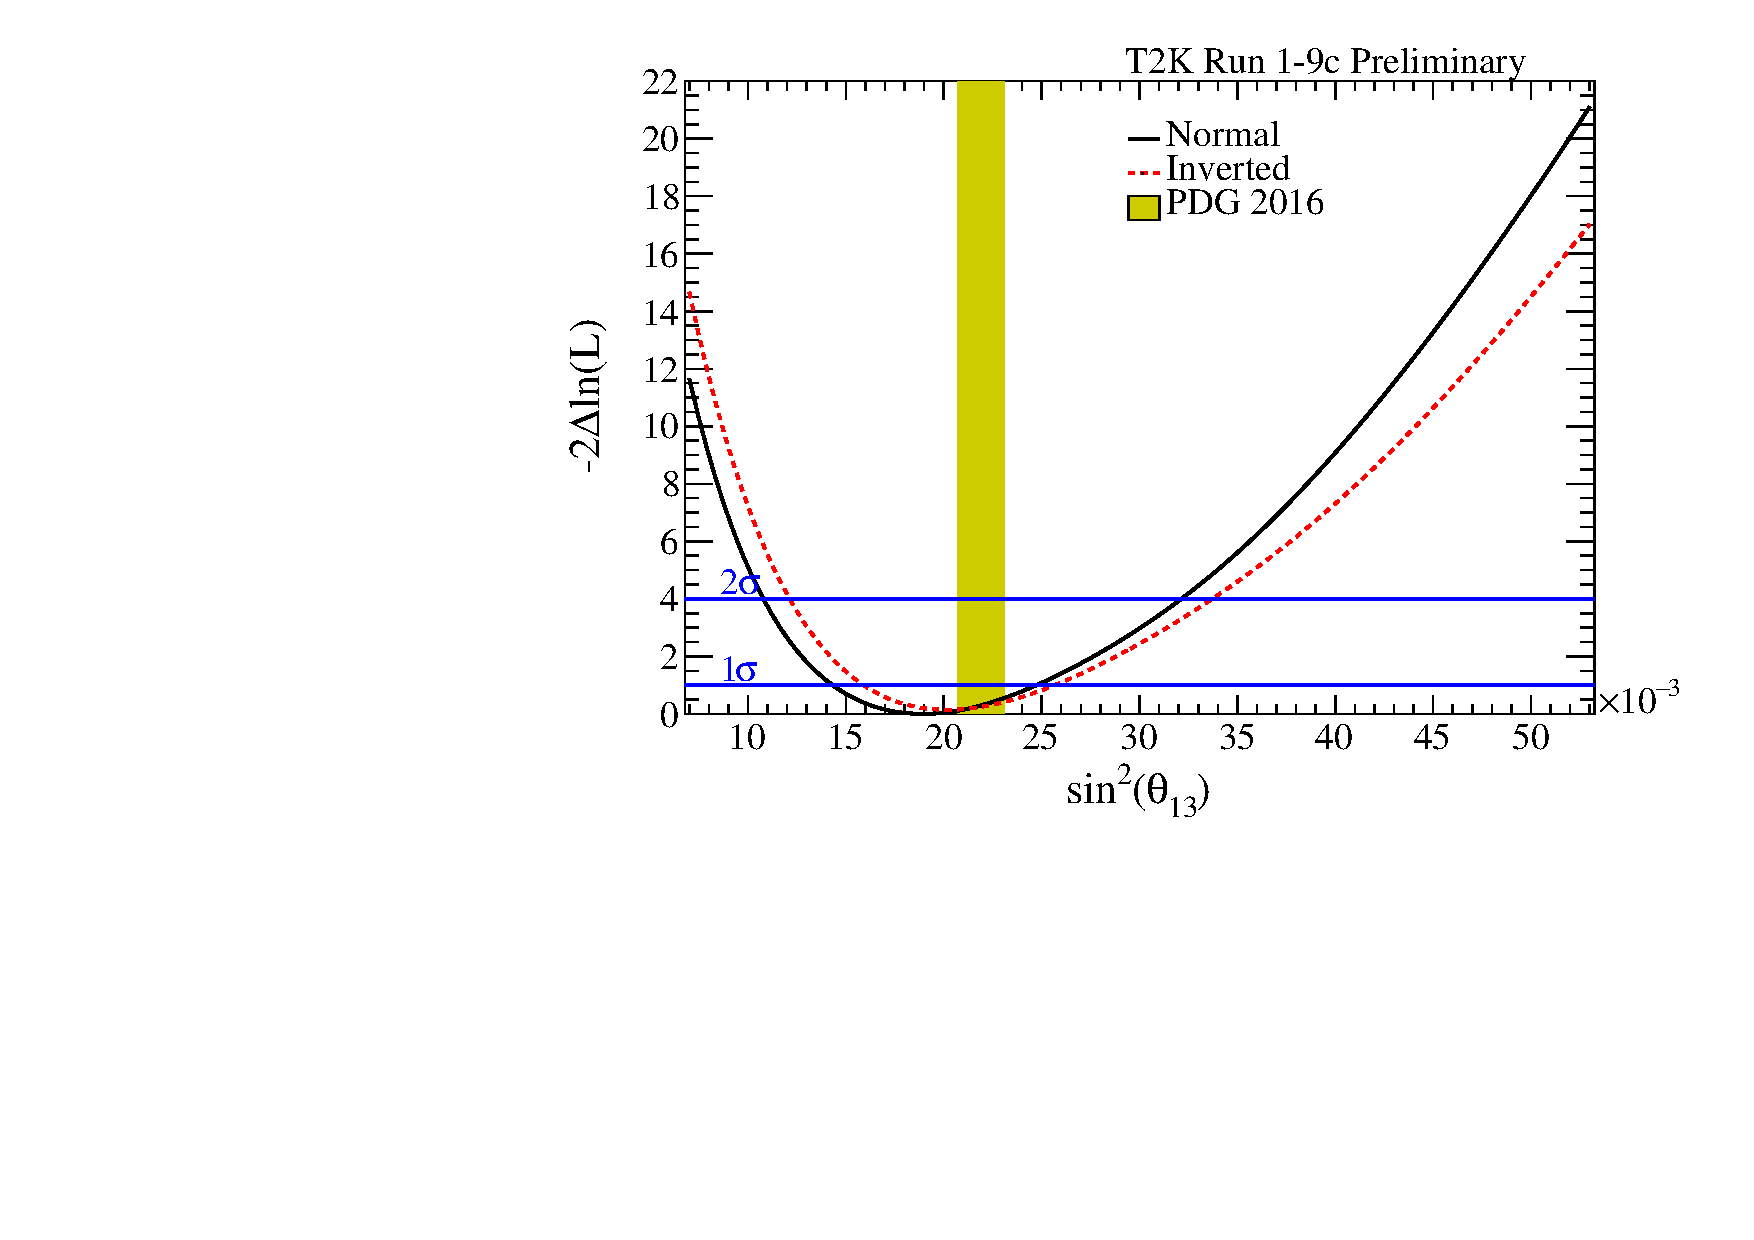
\includegraphics[width=0.9\textwidth]{images/sensitivity/mixing13_AsimovB_t2k_global}
		\caption{Asimov B \ssqthonethree T2K only}
	\end{subfigure}
	\caption {
		The expected $\Delta\chi^2$ distribution as a function of \ssqthonethree without reactor constraint for Asimov data sets A and B. The mass hierarchy is minimized, with normal and inverted hierarchy $\Delta\chi^2$ distributions shifted to the same global best-fit $\chi^2$ value, which is taken to be the minimum between normal and inverted hierarchy. All 5 samples were used to produce these fits.
	}
	\label{fig:th13_sensitivity}
\end{figure*}
\clearpage
\subsubsection{Results for \ssqthtwothree}

The sensitivity to \ssqthtwothree with reactor constraint and T2K only is shown for the Asimov data sets A and B in fig.~\ref{fig:th23_sensitivity}.

\begin{figure*}[htb]
	\center
	\begin{subfigure}[b]{0.49\textwidth}
		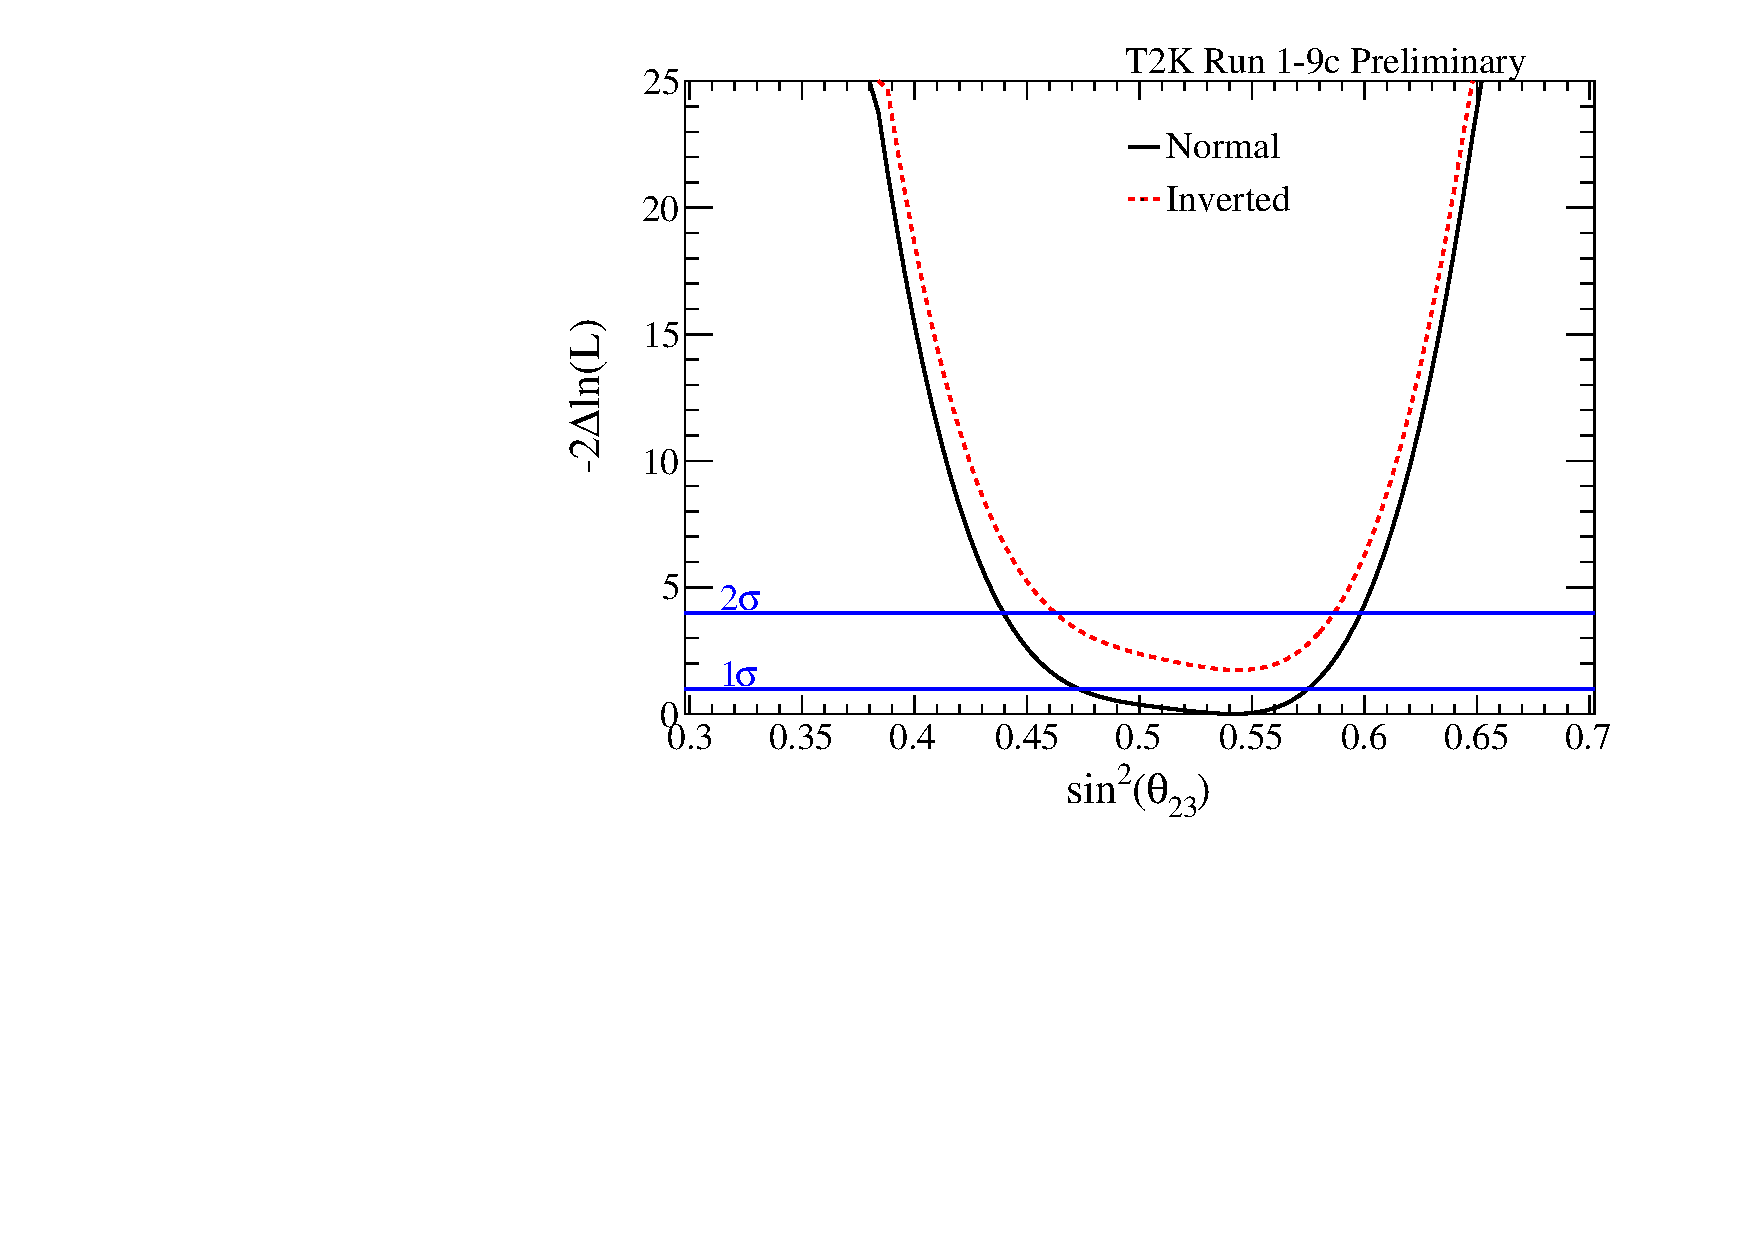
\includegraphics[width=0.9\textwidth]{images/sensitivity/mixing23_AsimovA_reactor_global}
		\caption{Asimov A \ssqthtwothree with reactor constraint}
	\end{subfigure}
	\begin{subfigure}[b]{0.49\textwidth}
		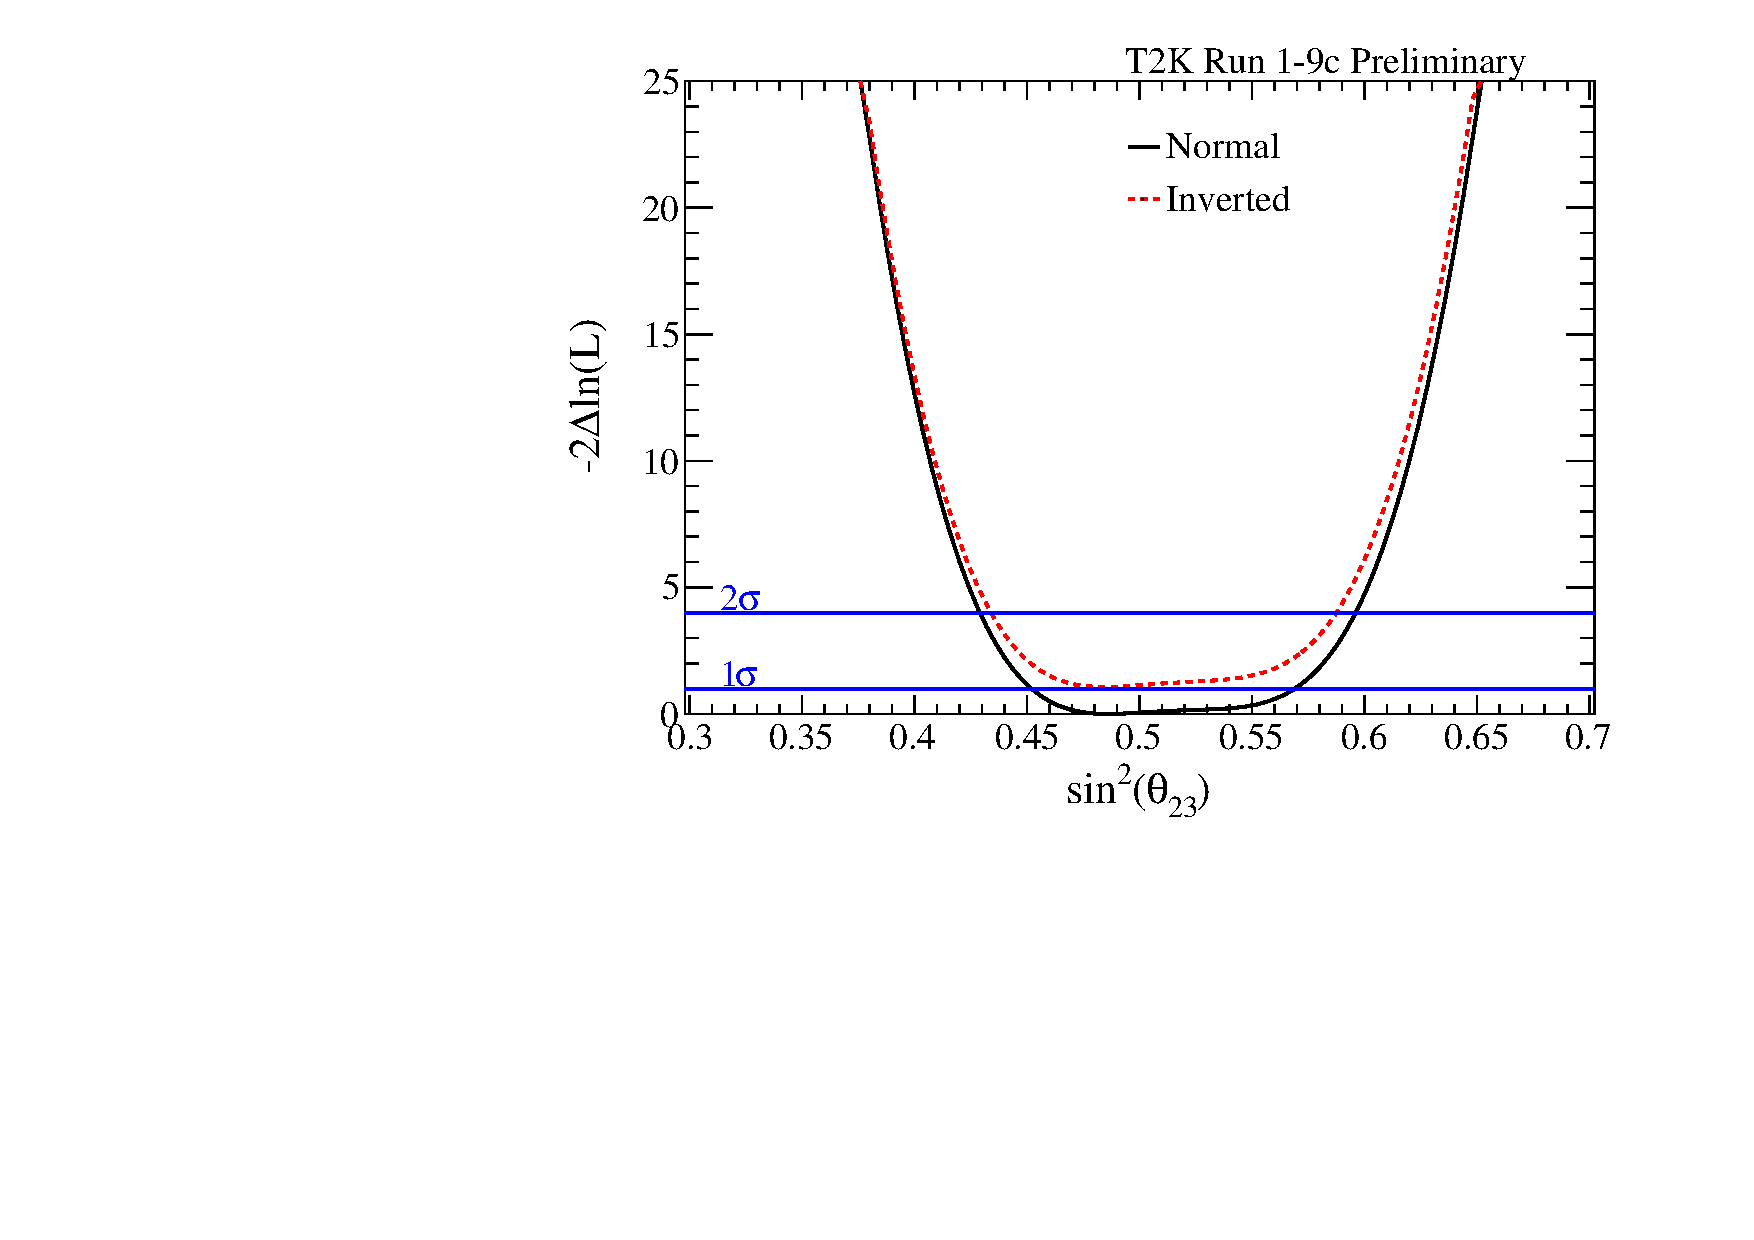
\includegraphics[width=0.9\textwidth]{images/sensitivity/mixing23_AsimovA_t2k_global}
		\caption{Asimov A \ssqthtwothree T2K only}
	\end{subfigure}
	\begin{subfigure}[b]{0.49\textwidth}
		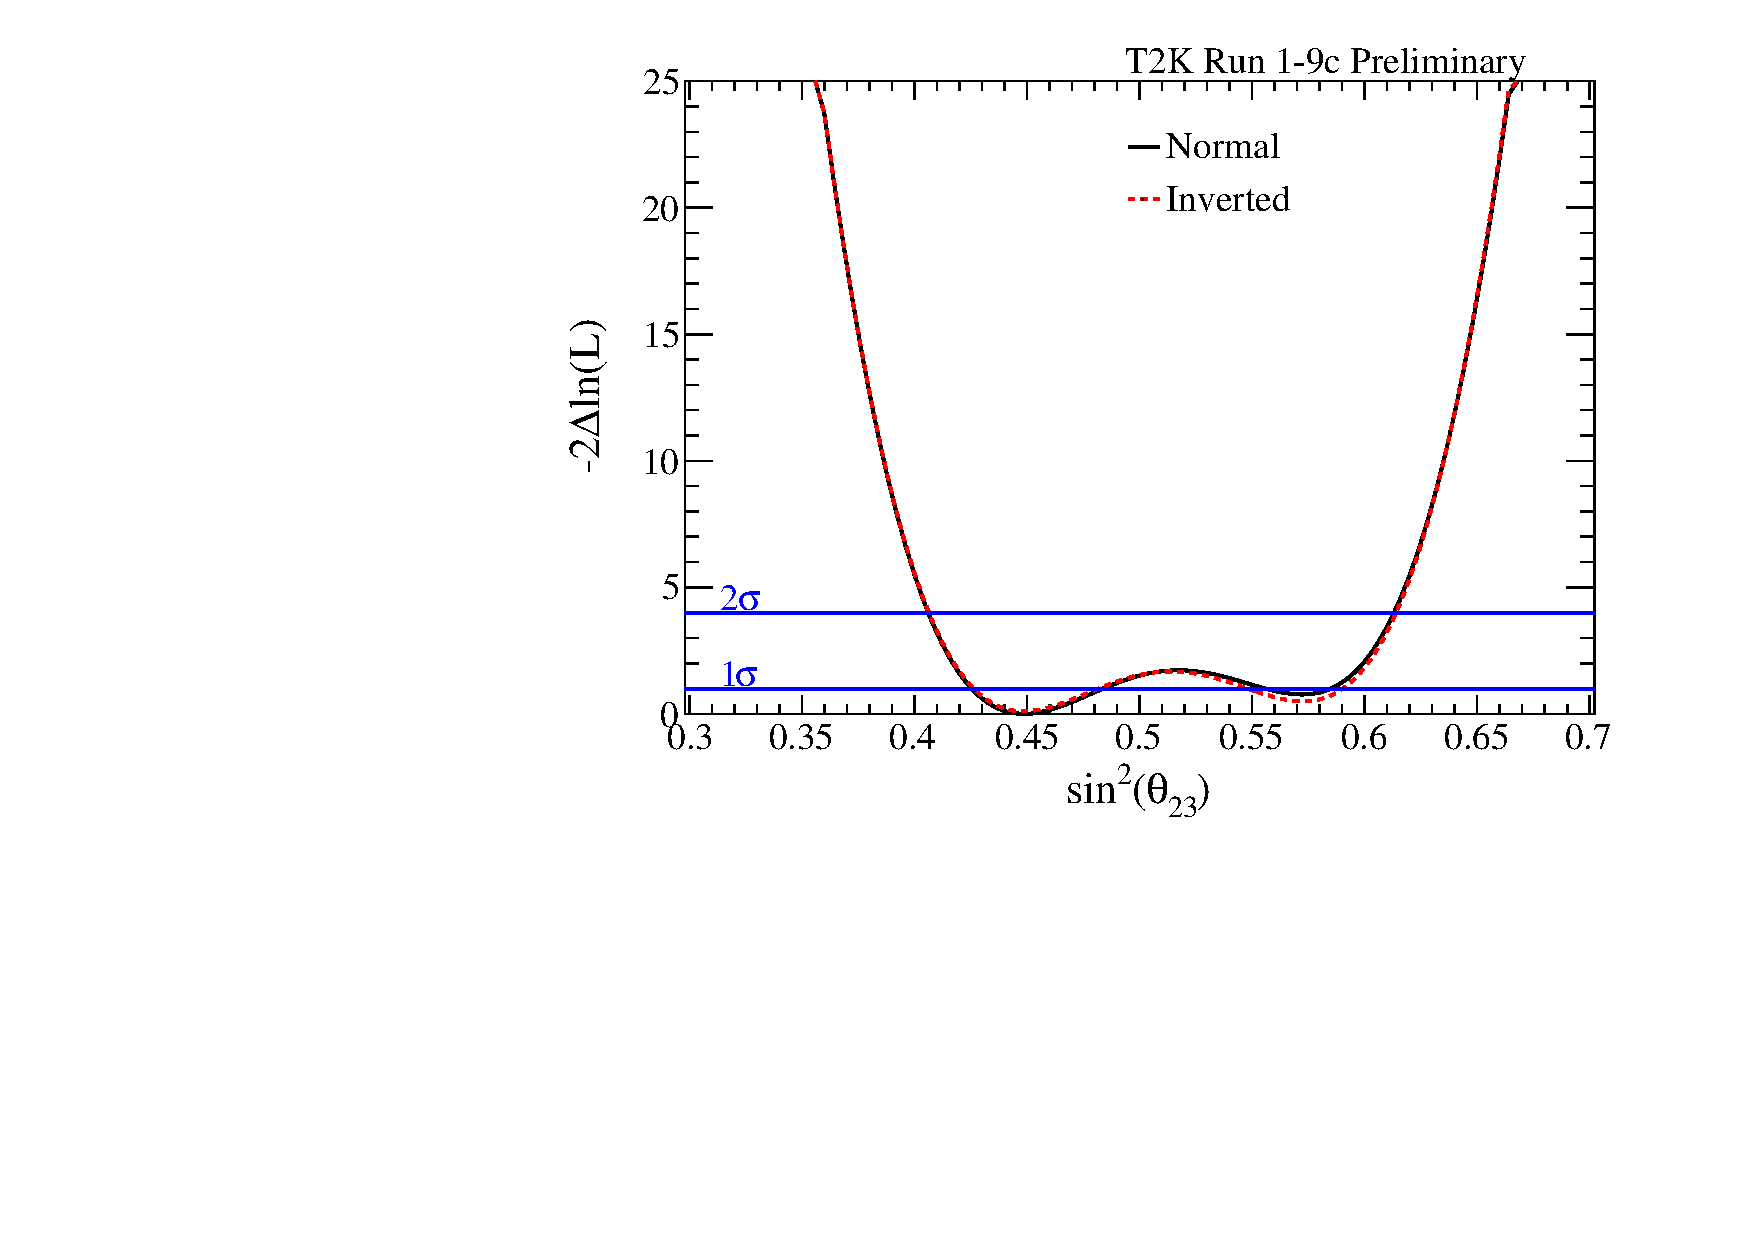
\includegraphics[width=0.9\textwidth]{images/sensitivity/mixing23_AsimovB_reactor_global}
		\caption{Asimov B \ssqthtwothree with reactor constraint}
	\end{subfigure}
	\begin{subfigure}[b]{0.49\textwidth}
		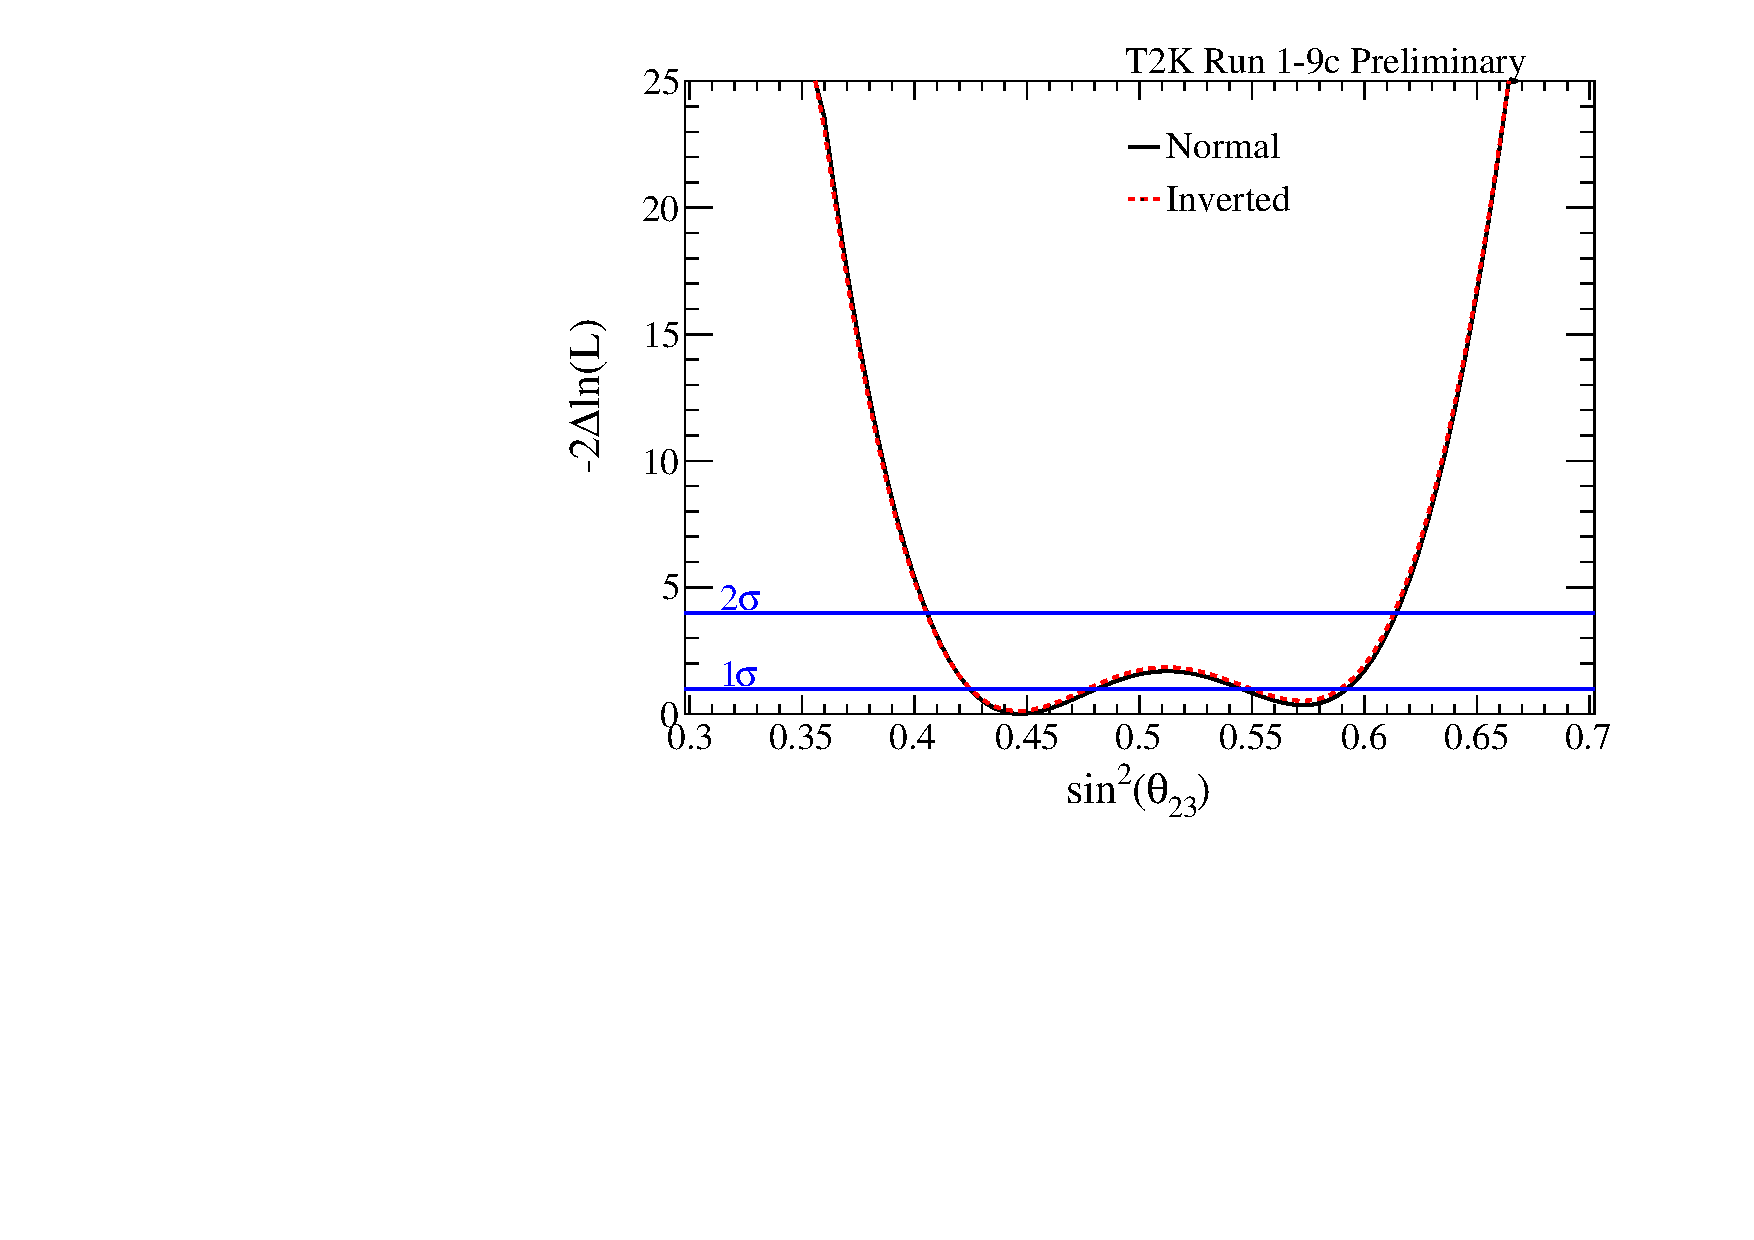
\includegraphics[width=0.9\textwidth]{images/sensitivity/mixing23_AsimovB_t2k_global}
		\caption{Asimov B \ssqthtwothree T2K only}
	\end{subfigure}
	\caption {
		The expected $\Delta\chi^2$ distribution as a function of \ssqthtwothree with and without reactor constraint for Asimov data sets A and B. The mass hierarchy is minimized, with normal and inverted hierarchy $\Delta\chi^2$ distributions shifted to the same global best-fit $\chi^2$ value, which is taken to be the minimum between normal and inverted hierarchy. All 5 samples were used to produce these fits.
	}
	\label{fig:th23_sensitivity}
\end{figure*}
\clearpage
\subsubsection{Results for \dmsq}

The sensitivity to \dmsq with reactor constraint and T2K only is shown for the Asimov data sets A and B in fig.~\ref{fig:dmsq23_sensitivity}.

\begin{figure*}[htb]
	\center
	\begin{subfigure}[b]{0.49\textwidth}
		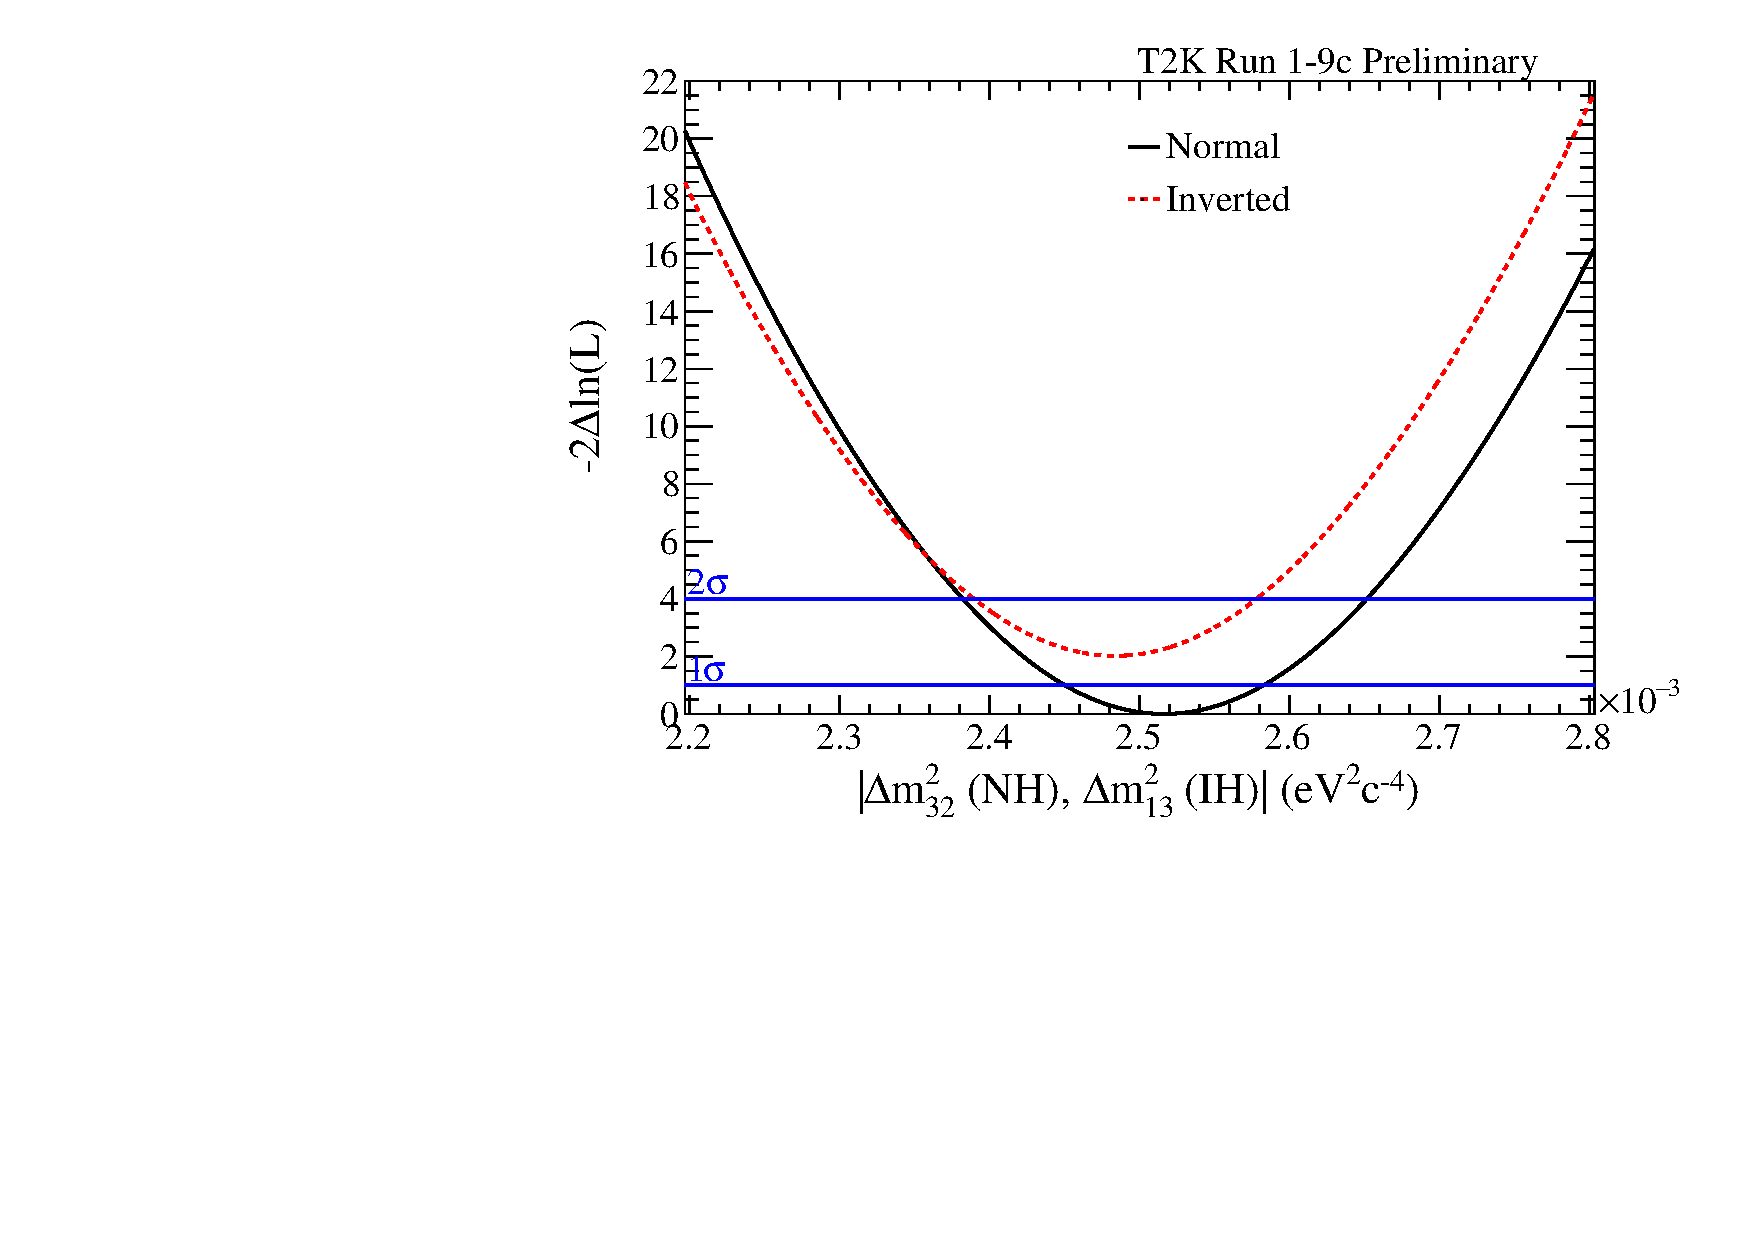
\includegraphics[width=0.9\textwidth]{images/sensitivity/dmsq23_AsimovA_reactor_global}
		\caption{Asimov A \dmsq with reactor constraint}
	\end{subfigure}
	\begin{subfigure}[b]{0.49\textwidth}
		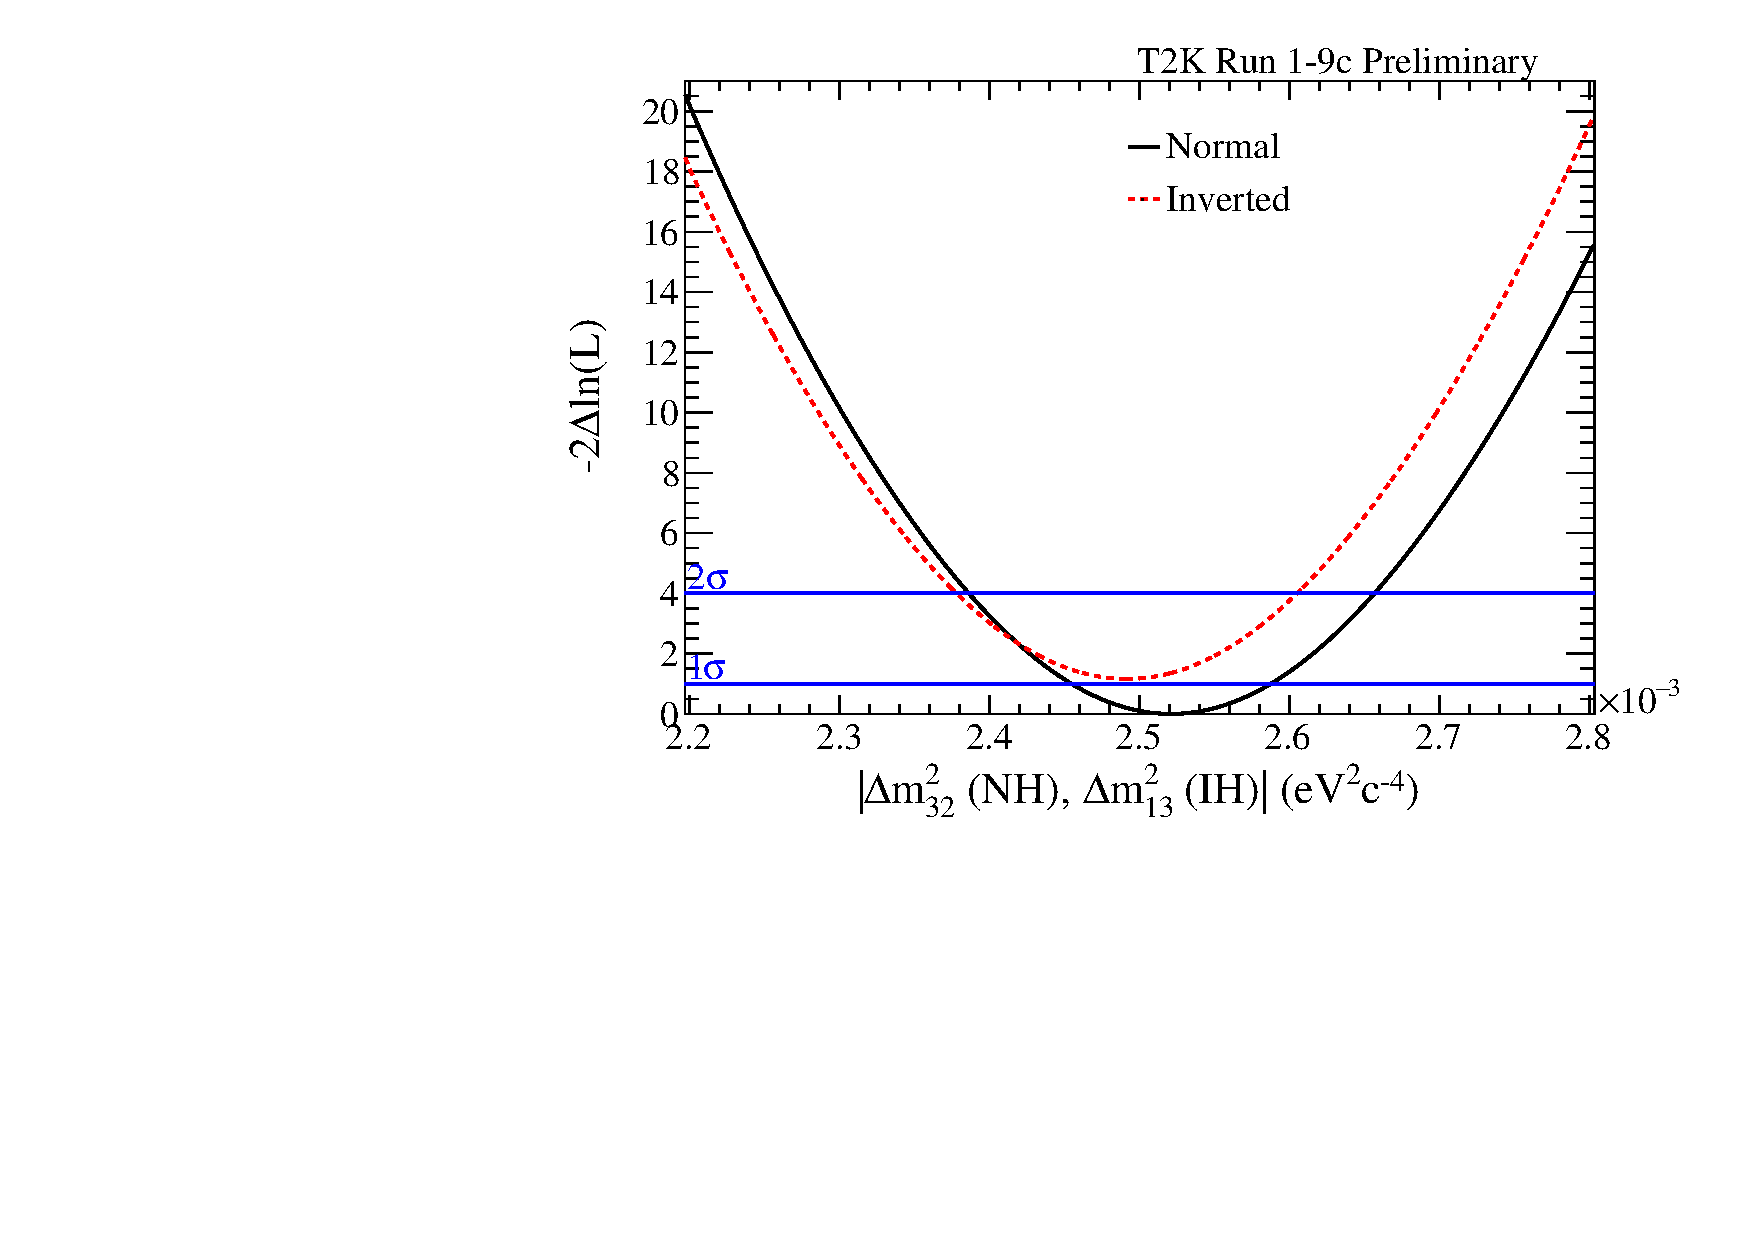
\includegraphics[width=0.9\textwidth]{images/sensitivity/dmsq23_AsimovA_t2k_global}
		\caption{Asimov A \dmsq T2K only}
	\end{subfigure}
	\begin{subfigure}[b]{0.49\textwidth}
		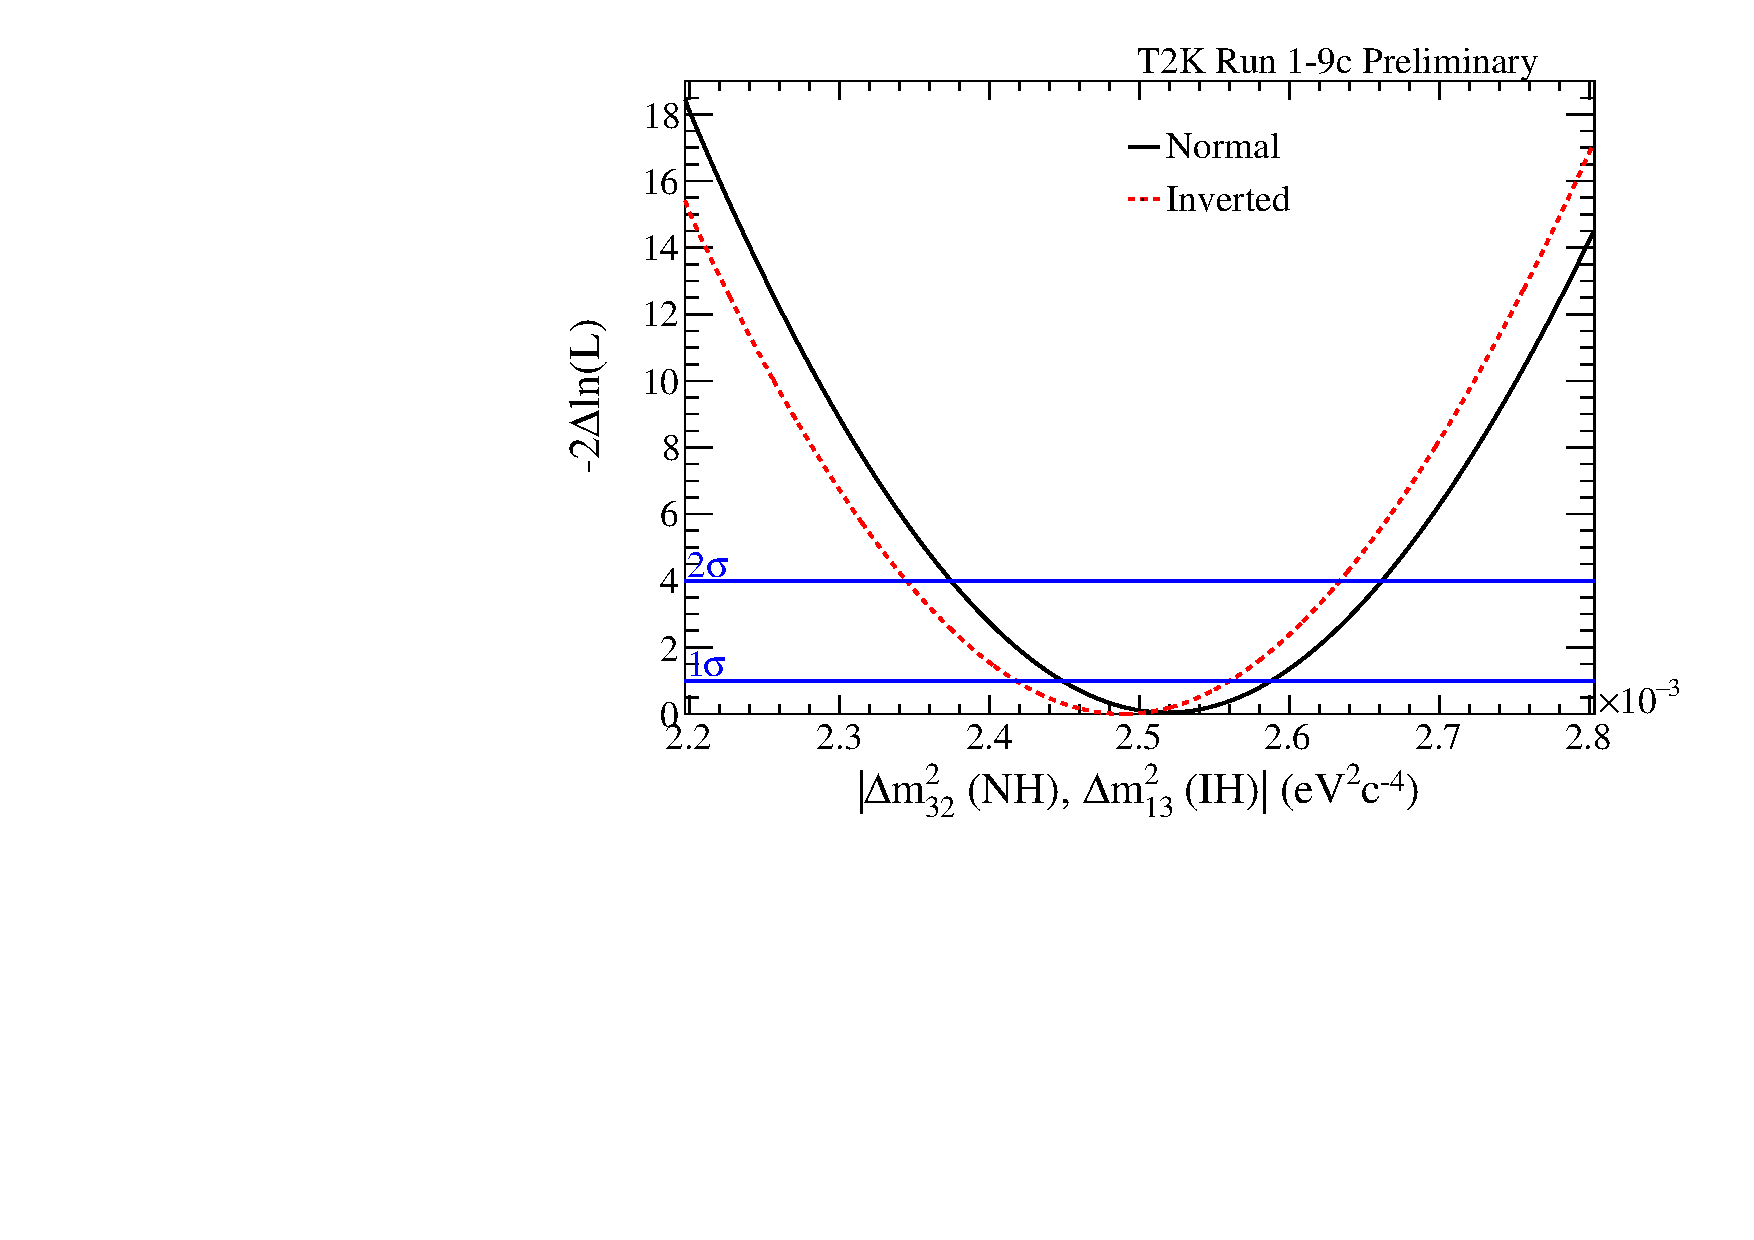
\includegraphics[width=0.9\textwidth]{images/sensitivity/dmsq23_AsimovB_reactor_global}
		\caption{Asimov B \dmsq with reactor constraint}
	\end{subfigure}
	\begin{subfigure}[b]{0.49\textwidth}
		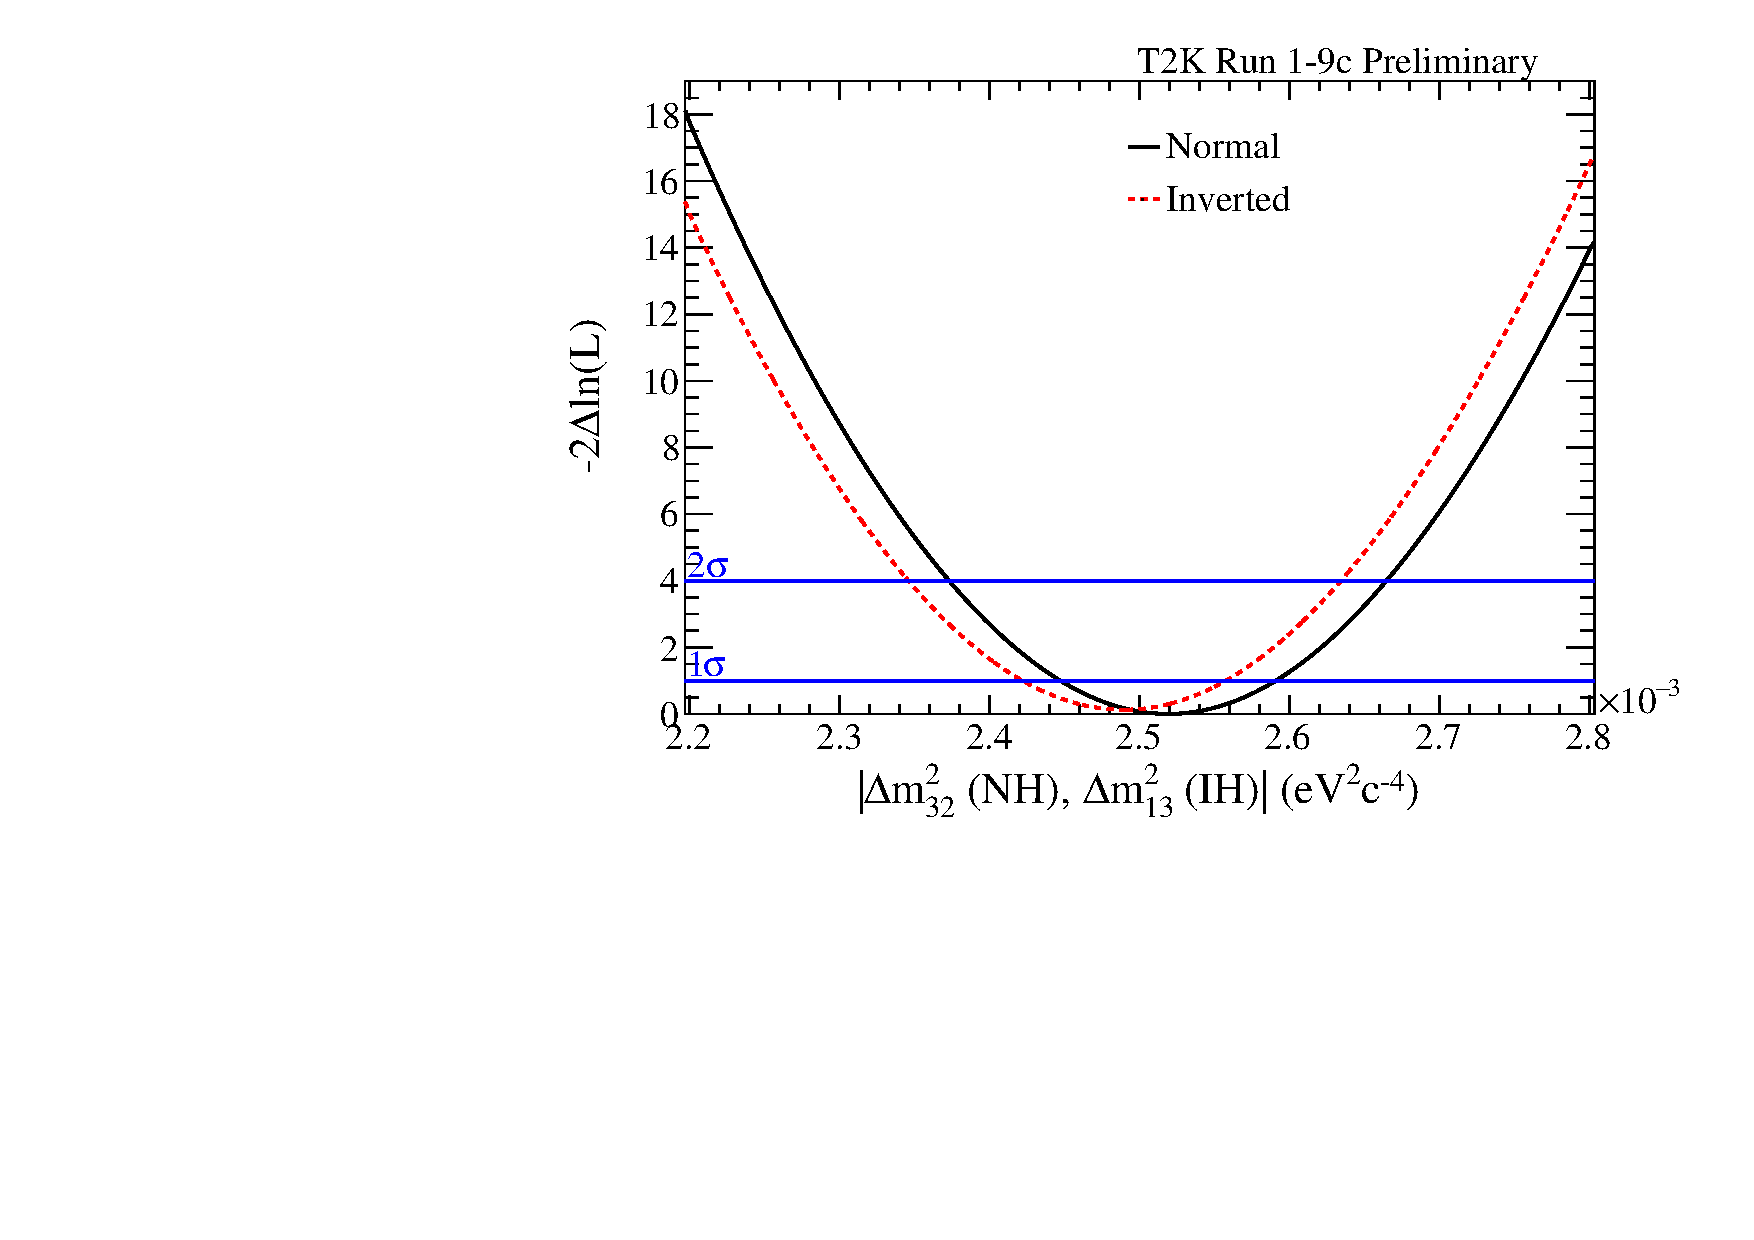
\includegraphics[width=0.9\textwidth]{images/sensitivity/dmsq23_AsimovB_t2k_global}
		\caption{Asimov B \dmsq T2K only}
	\end{subfigure}
	\caption {
		The expected $\Delta\chi^2$ distribution as a function of \dmsq with and without reactor constraint for Asimov data sets A and B. The mass hierarchy is minimized, with normal and inverted hierarchy $\Delta\chi^2$ distributions shifted to the same global best-fit $\chi^2$ value, which is taken to be the minimum between normal and inverted hierarchy. All 5 samples were used to produce these fits.
	}
	\label{fig:dmsq23_sensitivity}
\end{figure*}

\clearpage

\section {Results of the $\nu\bar{\nu}$ joint analysis with the \RunPeriod dataset}
\label{sec:results}

The results of the \RunPeriod data set fit, for an exposure of \TotalPotNu POT in neutrino mode and of \TotalPotNuBar POT in antineutrino mode, are shown in this chapter. In \cref{fig:asimovpf_spectra_mc_data} the predicted spectra of $\mu$-like and $e$-like samples are compared to the observed data. In \cref{tab:num_events_run19c} the expected and observed number of events in \RunPeriod data set are shown. The predicted number of events are shown for the oscillation parameters of Asimov data sets A and B. The comparison of the confidence intervals obtained by the fit of the \RunPeriod data set among all the oscillation analysis groups is shown in \cref{app:group_comparison}.

\begin{table}[htb]
\centering
\begin{adjustbox}{width=\textwidth, totalheight=\textheight, keepaspectratio}
\begin{tabular}{| c | c | c | c | c | c | c |}
\hline
Beam mode & Sample & Exp. Asimov A & Exp. Asimov A & Exp. Asimov B & Exp. Not Osc & Observed \\
 & & & ($\delta_{CP}=0$) & & & \\
\hline
$\nu$ & $\mu$-like       & 268.535 & 268.232 & 281.182 & 1211.365 & \NskObservedNumu \\
$\nu$ & $e$-like         &  73.784 &  61.615 &  54.845 &   15.438 & \NskObservedNue \\
$\bar{\nu}$ & $\mu$-like &  95.535 &  95.306 &  98.108 &  314.277 & \NskObservedNumuBar \\
$\bar{\nu}$ & $e$-like   &  11.752 &  13.403 &  12.161 &    4.820 & \NskObservedNueBar \\
$\nu$ & \nueCConepi-like &   6.924 &   6.009 &   5.389 &    2.553 & \NskObservedNueCConepi \\
\hline
\end{tabular}

\end{adjustbox}
\caption{
The observed, expected and best-fit number of events in \RunPeriod data set for an exposure of \TotalPotNuRunOneEight POT in neutrino mode and of \TotalPotNuBarRunOneEight POT in antineutrino mode are shown 
for each selected sample. The prediction is produced using the BANFF tuning and the oscillation parameters shown in \cref{tab:asimov_definition1}.
}
\label{tab:num_events_run19c}
\end{table}

The predicted and observed spectra are shown for each of the samples in \cref{fig:asimovpf_spectra_mc_data}. The $e$-like samples are broken down into $E_\text{rec}$ and $\theta$ projections in \cref{fig:asimovpf_spectra_mc_data_elike_1D}.
\begin{figure*}[htb]
	\center
	\begin{subfigure}[b]{0.49\textwidth}
		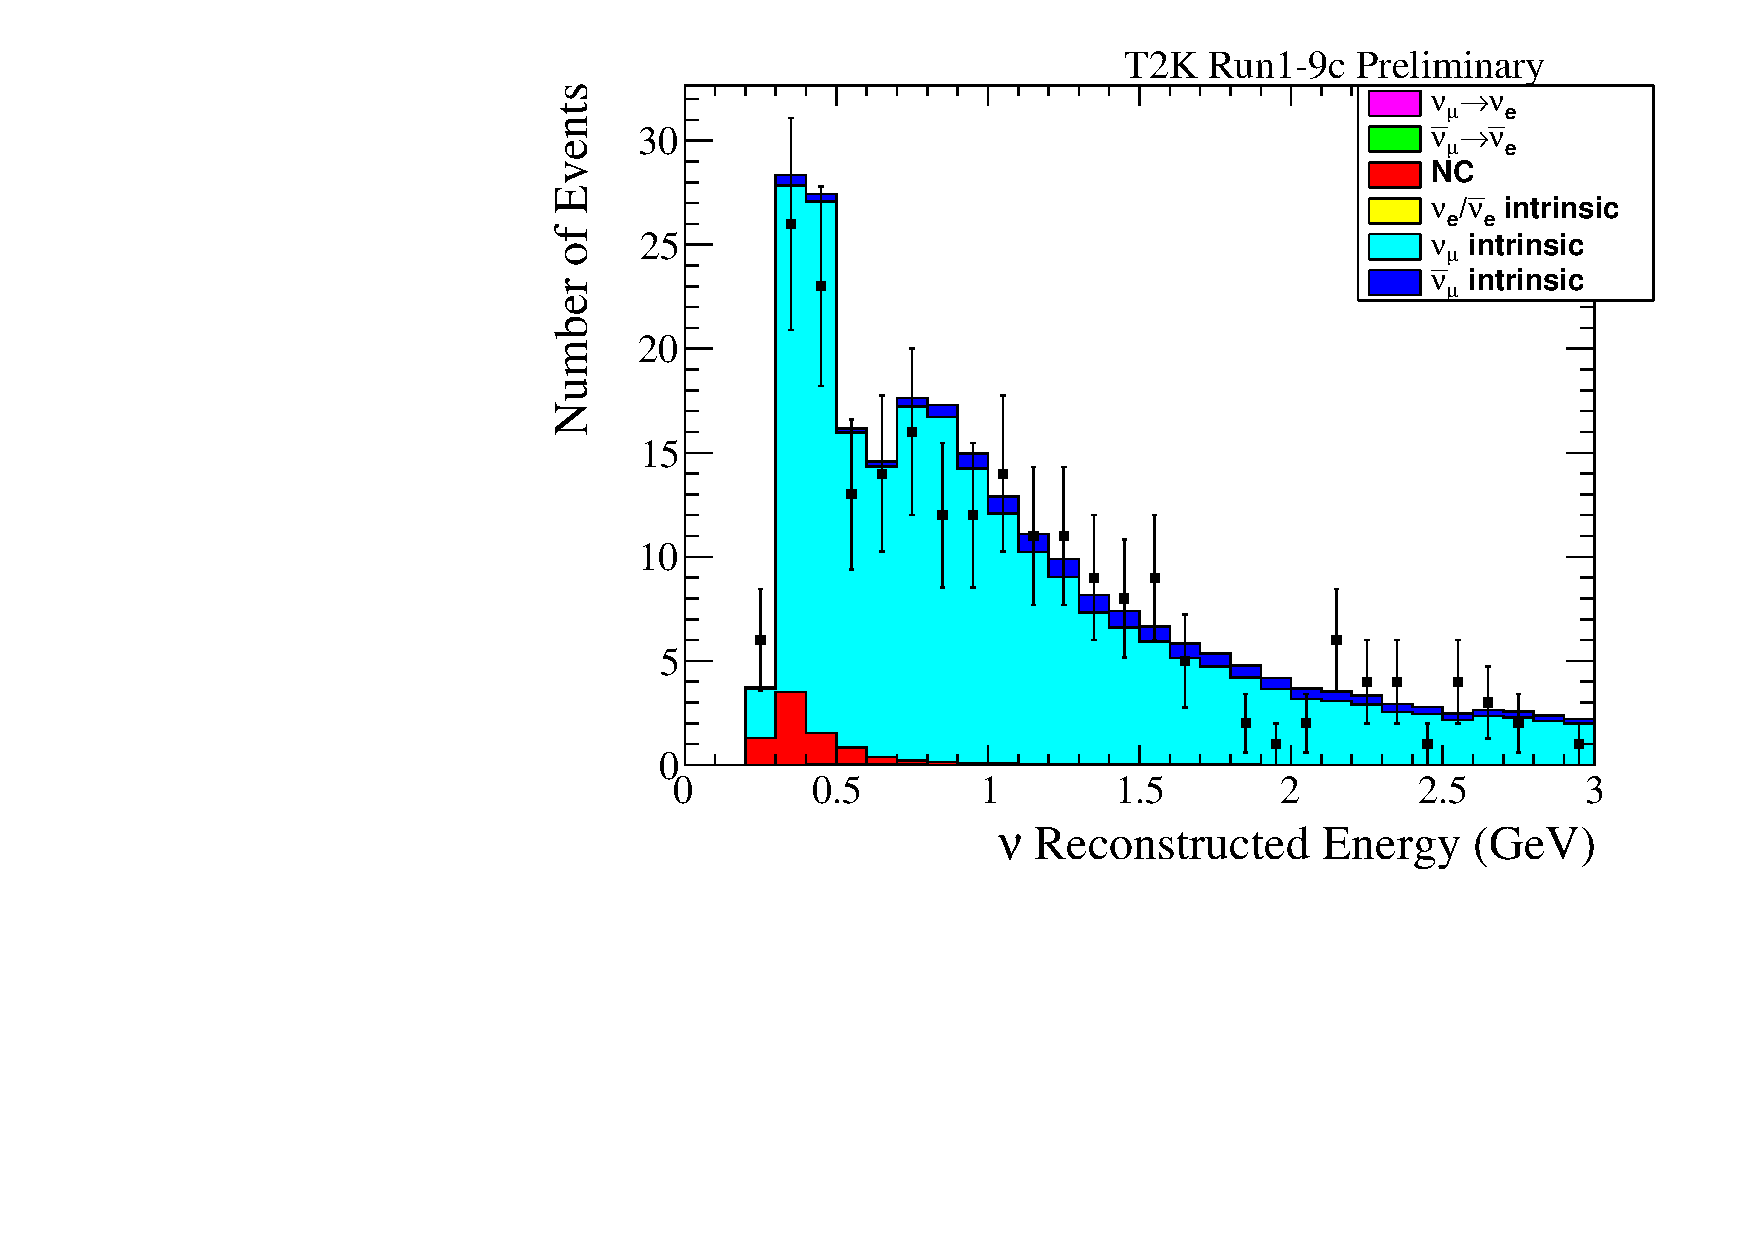
\includegraphics[width=0.9\textwidth]{images/spectra/data/spectrum_asimov2018_1Rmu_data}
		\caption{Muon-like, neutrino mode}
	\end{subfigure}
	\begin{subfigure}[b]{0.49\textwidth}
		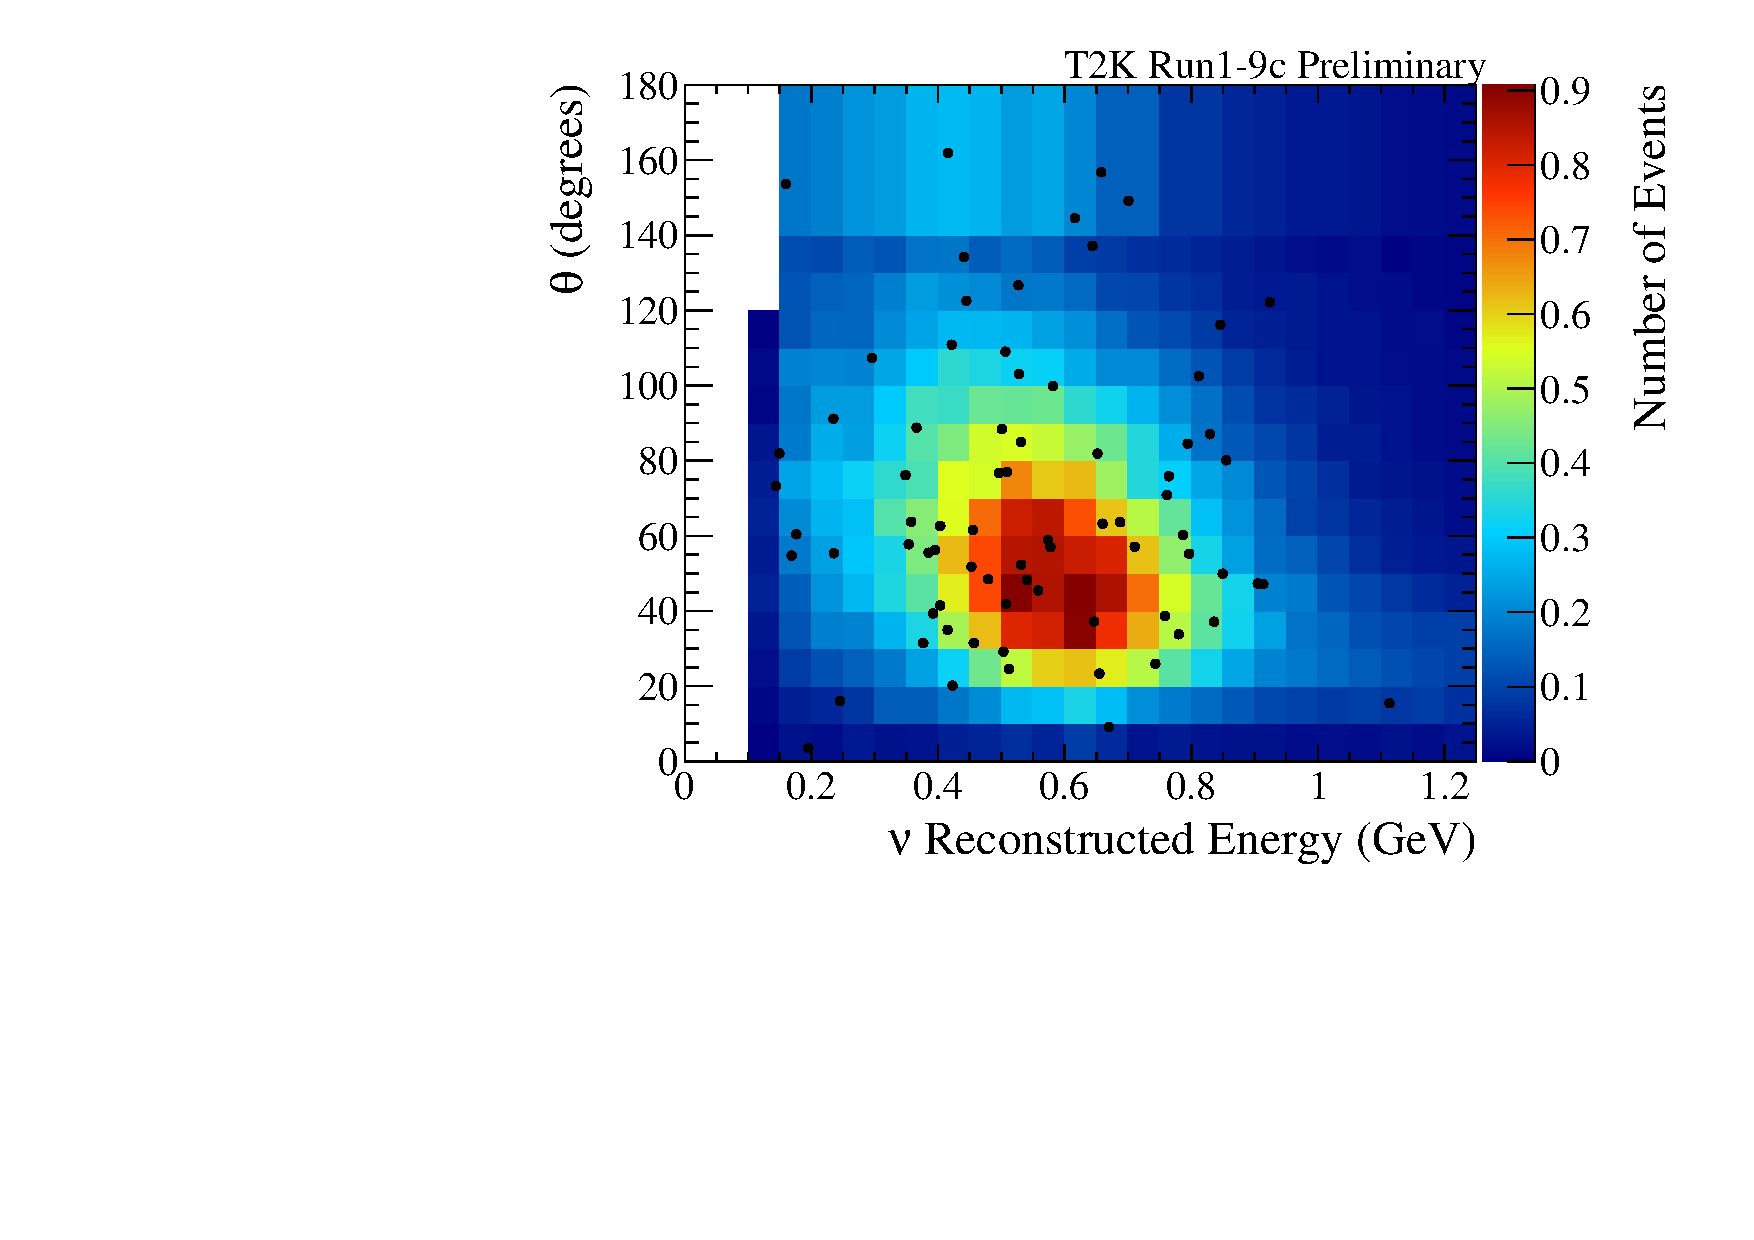
\includegraphics[width=0.9\textwidth]{images/spectra/data/spectrum_asimov2018_1Re_data}
		\caption{Electron-like, neutrino mode}
	\end{subfigure}
	\begin{subfigure}[b]{0.49\textwidth}
		\includegraphics[width=0.9\textwidth]{images/spectra/data/spectrum_asimov2018_RHC1Rmu_data}
		\caption{Muon-like, antineutrino mode}
	\end{subfigure}
	\begin{subfigure}[b]{0.49\textwidth}
		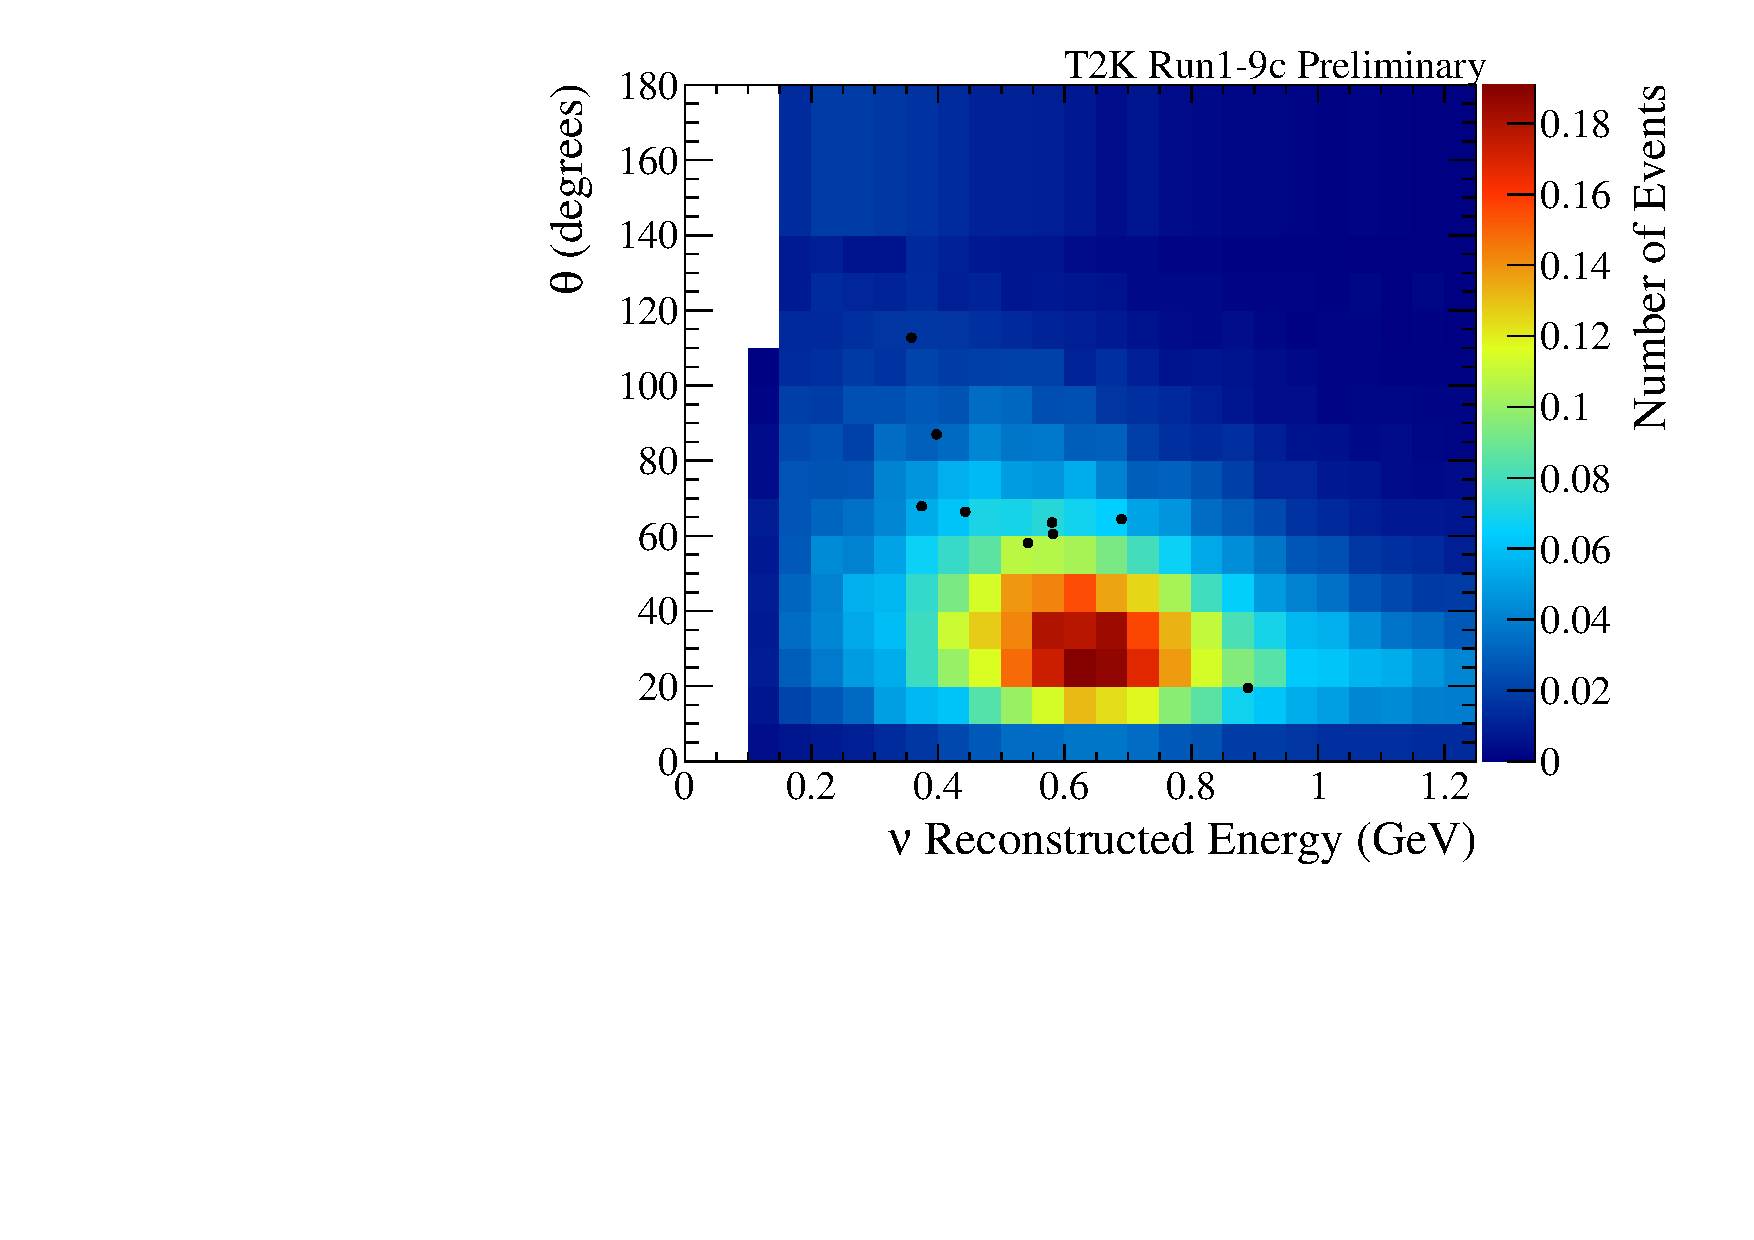
\includegraphics[width=0.9\textwidth]{images/spectra/data/spectrum_asimov2018_RHC1Re_data}
		\caption{Electron-like antineutrino mode}
	\end{subfigure}
	\begin{subfigure}[b]{0.49\textwidth}
		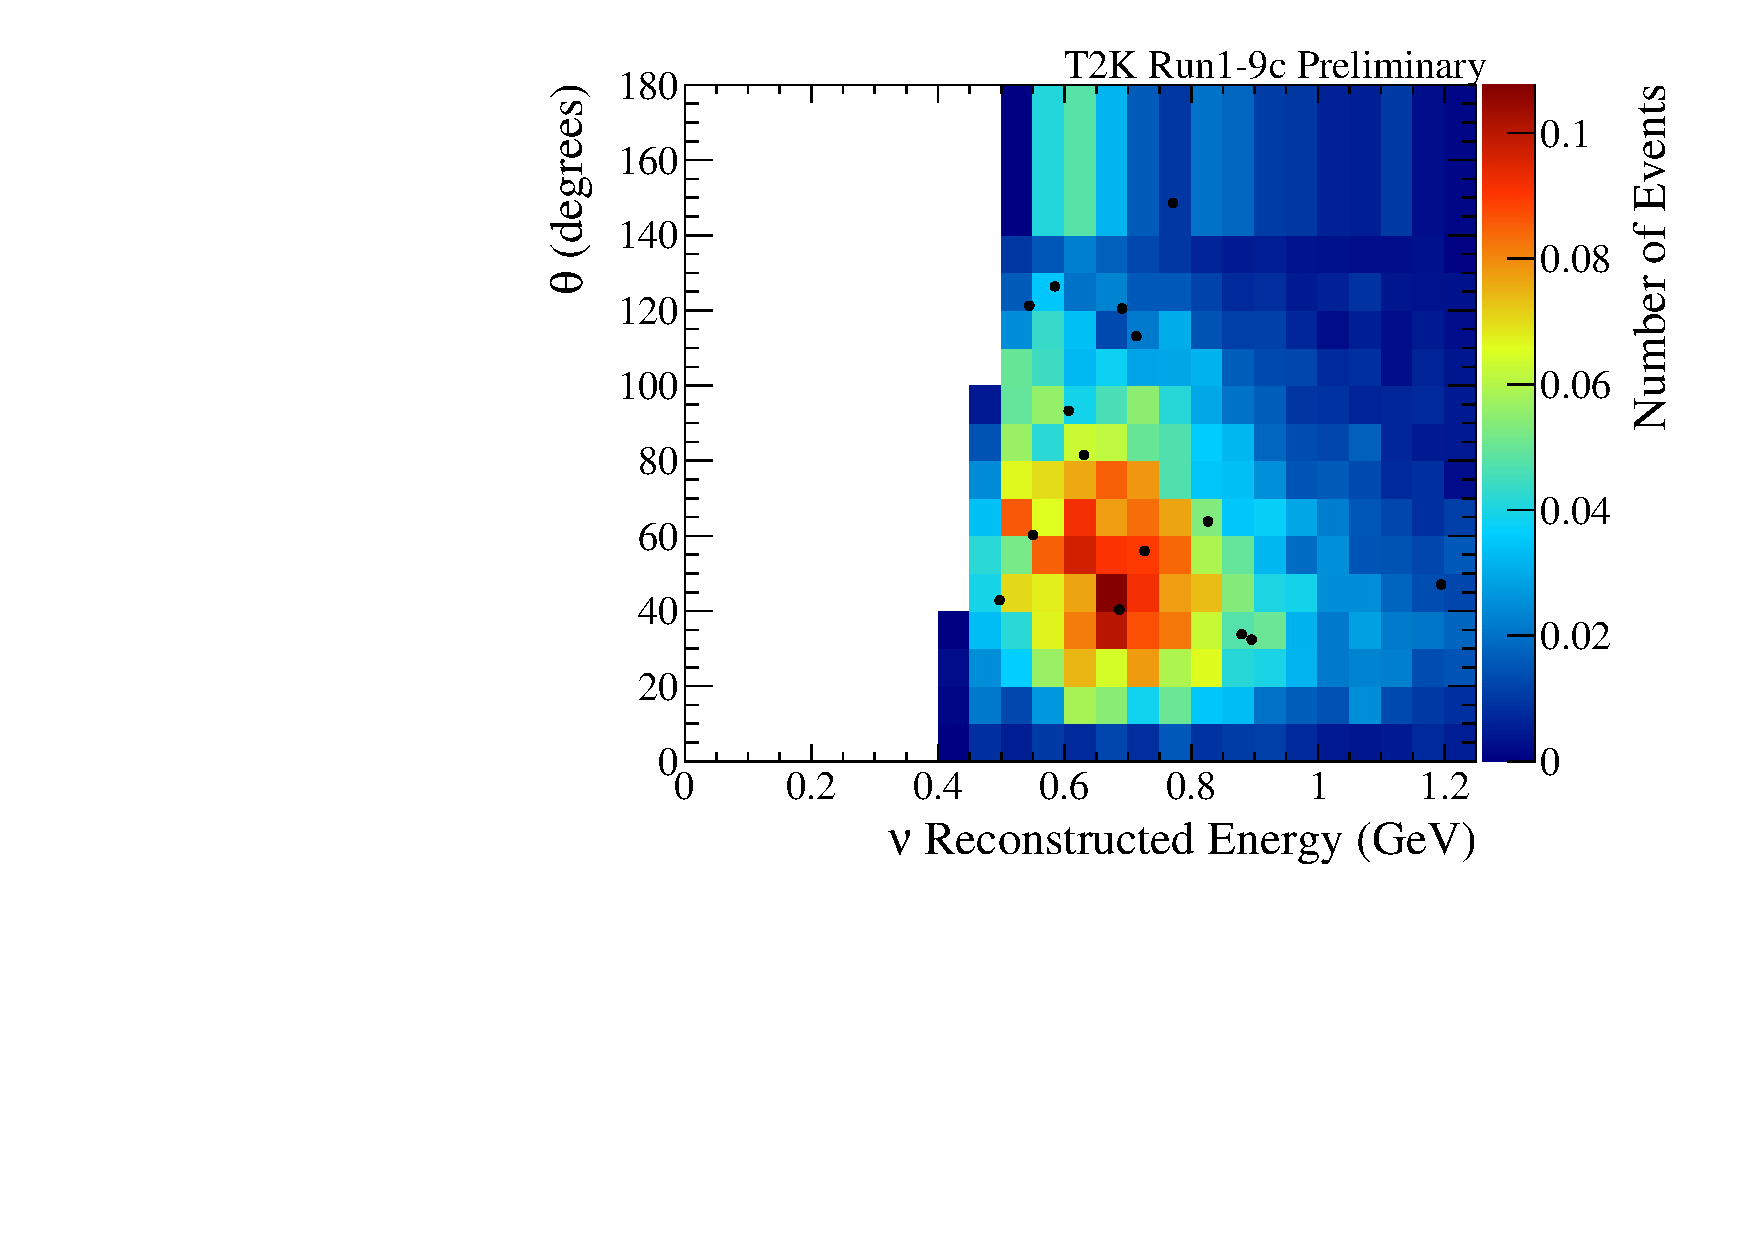
\includegraphics[width=0.9\textwidth]{images/spectra/data/spectrum_asimov2018_MultiRe_data}
		\caption{\nueCConepi-like, neutrino mode}
	\end{subfigure}
	\caption {
		Predicted spectra and observed events (points). $\mu$-like distributions are a function of the reconstructed neutrino energy, while the $e$-like, including \nueCConepi, distributions are functions of both the reconstructed neutrino energy and the reconstructed angle between the outgoing lepton and the neutrino direction. The distributions correspond to the statistics collected in the full \RunPeriod data set. The spectra are generated with the systematic parameters described in \cref{sec:systematics} and the oscillation parameters corresponding to the best-fit values from the data fit (solar parameters at PDG 2016).
	}
	\label{fig:asimovpf_spectra_mc_data}
\end{figure*}
\clearpage
\begin{figure*}[htb]
	\center

	\begin{subfigure}[b]{0.49\textwidth}
		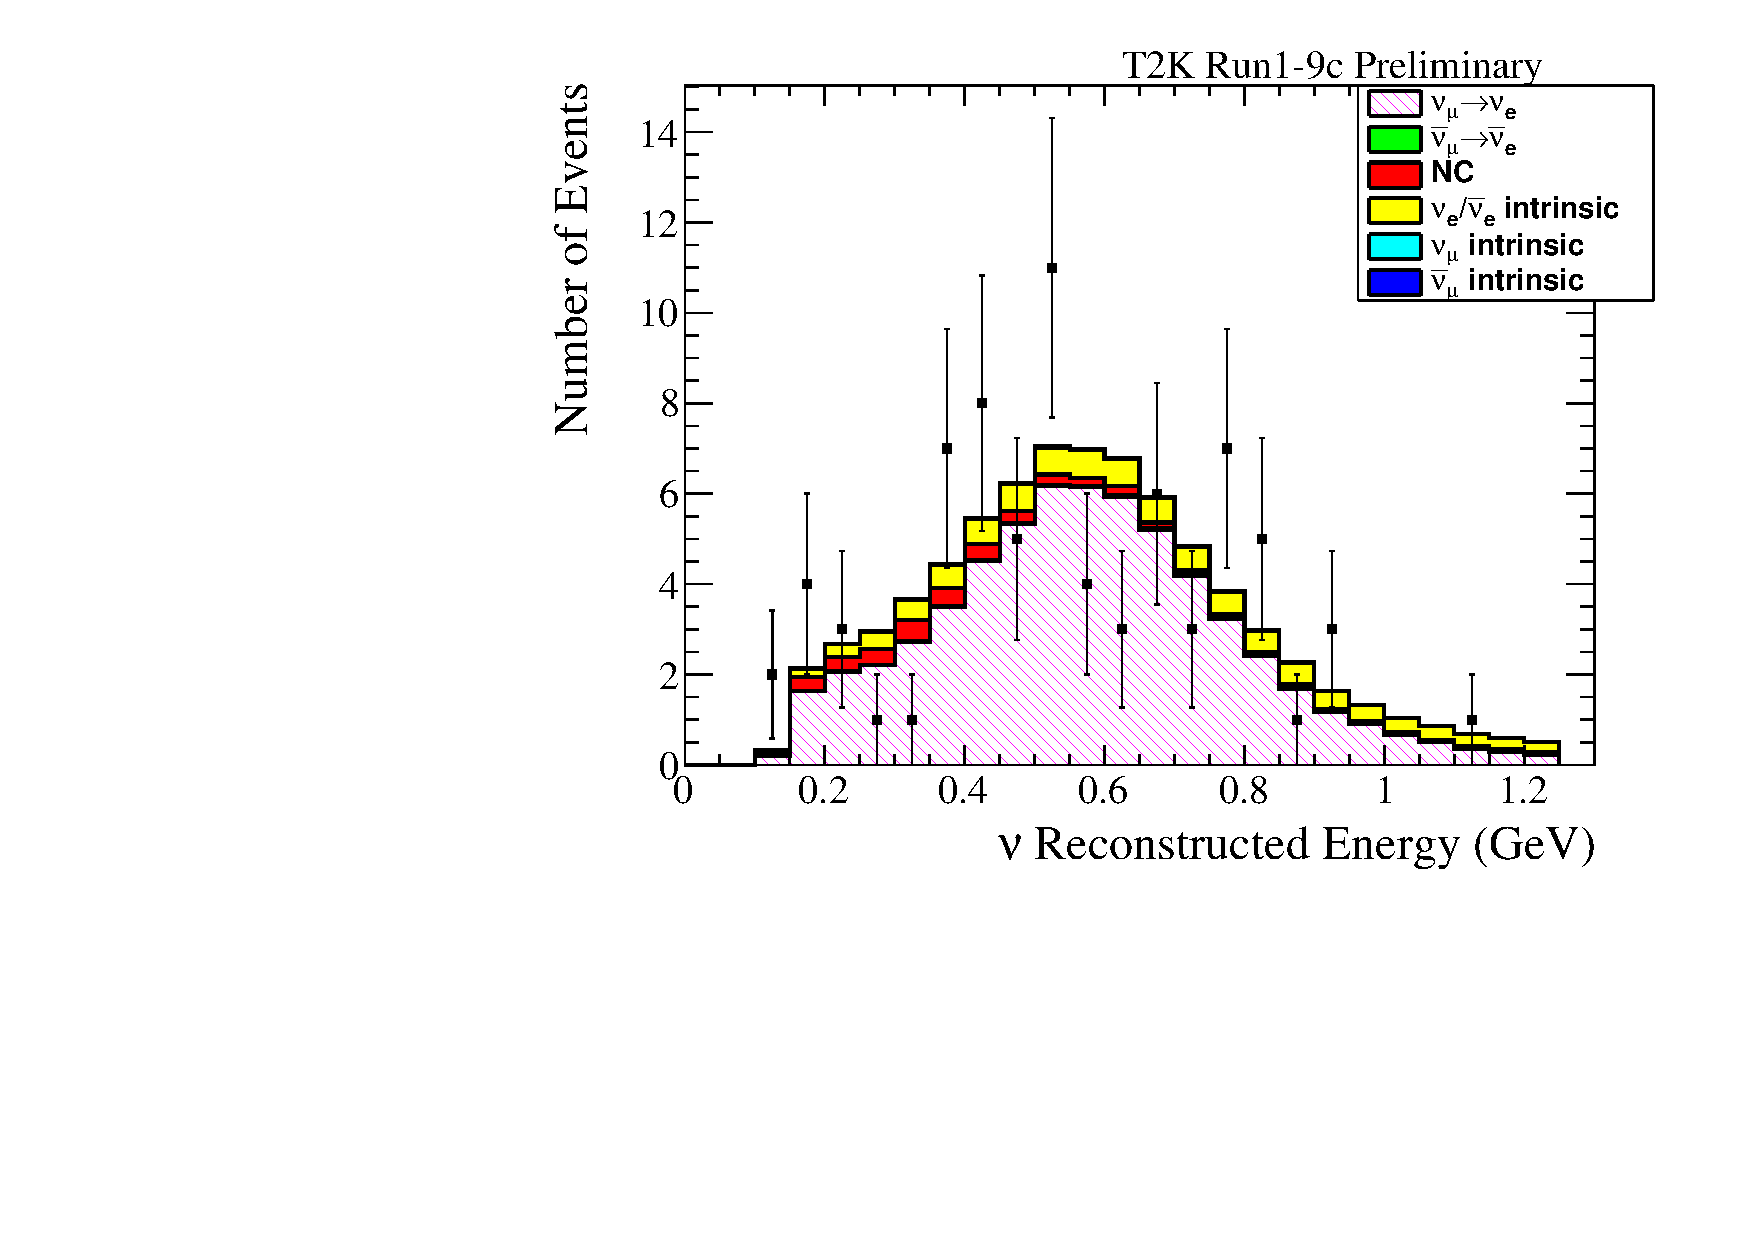
\includegraphics[width=0.9\textwidth]{images/spectra/data/erec_spectrum_asimov2018_1Re_data}
		\caption{Electron-like, neutrino mode}
	\end{subfigure}
	\begin{subfigure}[b]{0.49\textwidth}
		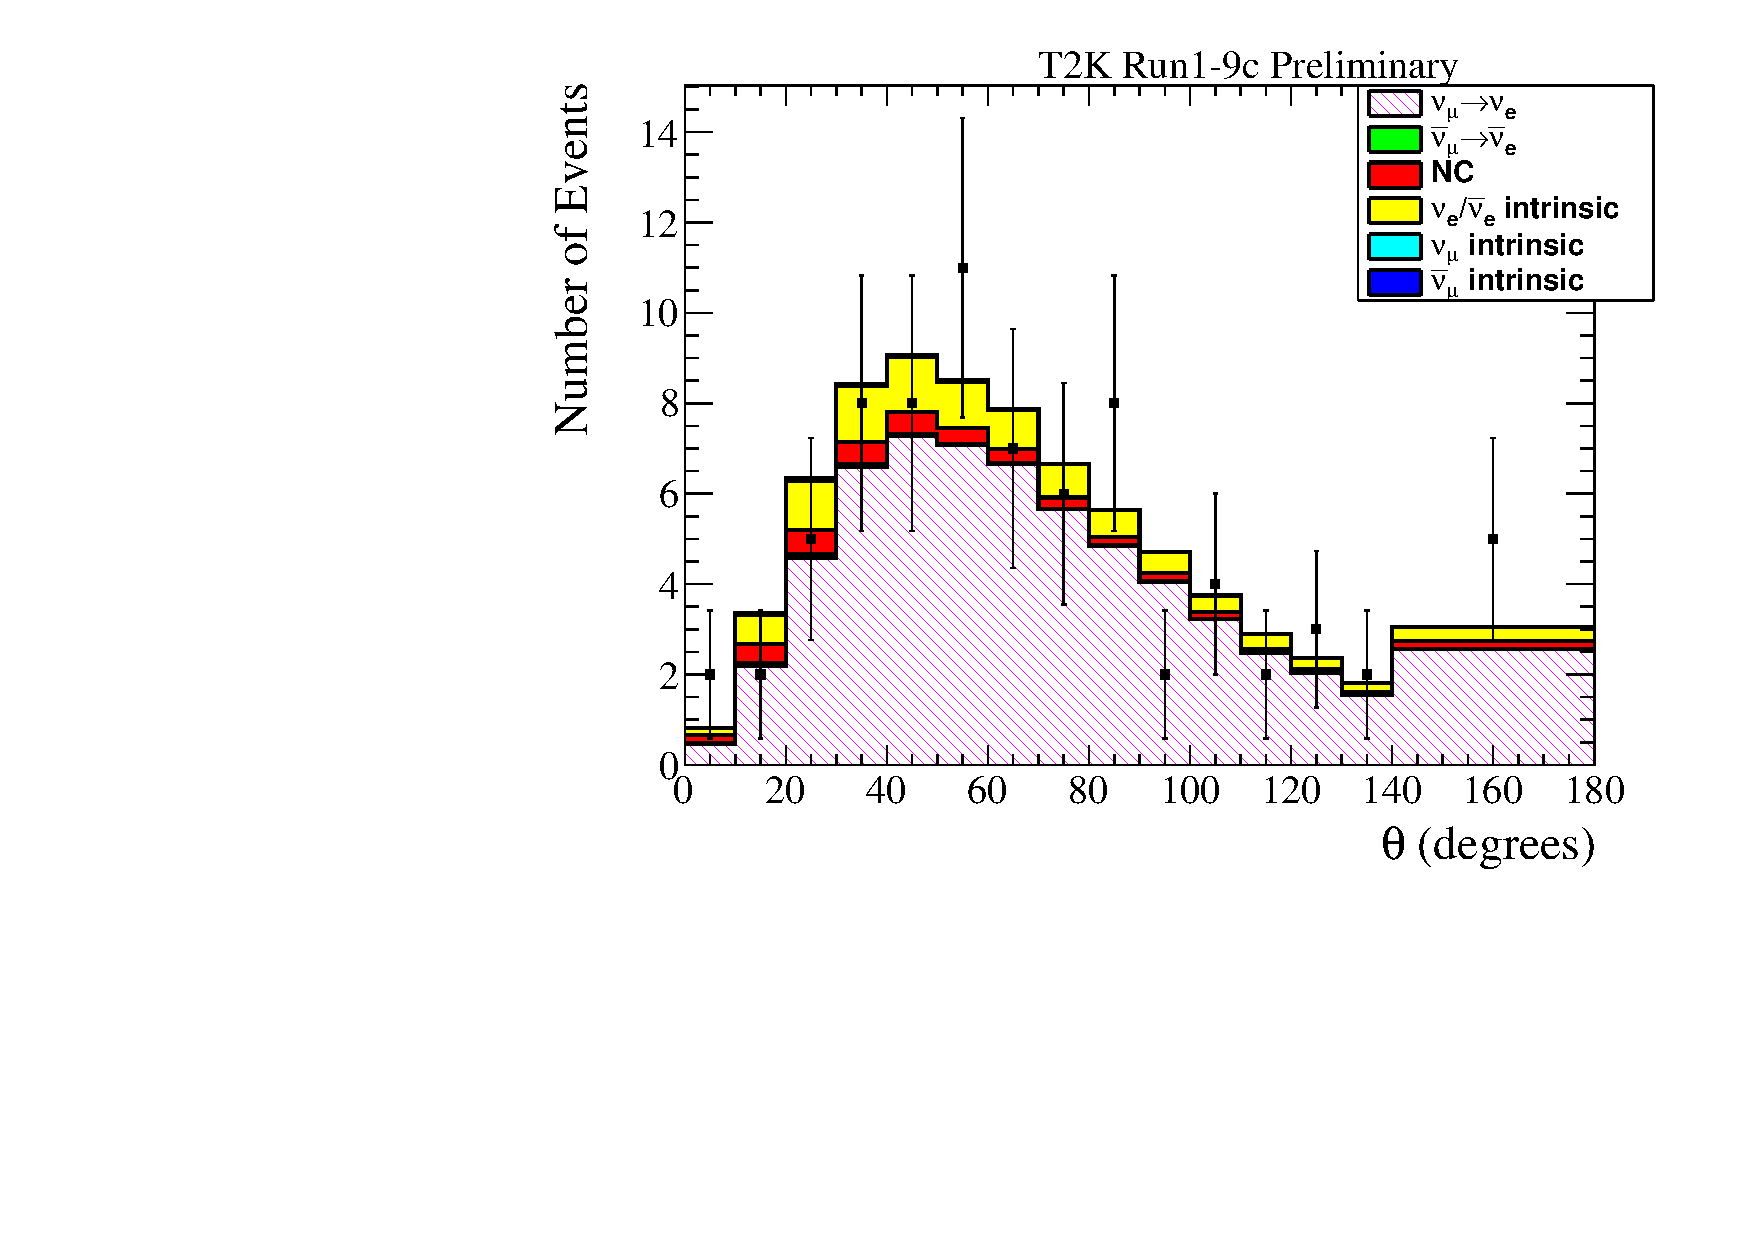
\includegraphics[width=0.9\textwidth]{images/spectra/data/theta_spectrum_asimov2018_1Re_data}
		\caption{Electron-like, neutrino mode}
	\end{subfigure}

	\begin{subfigure}[b]{0.49\textwidth}
		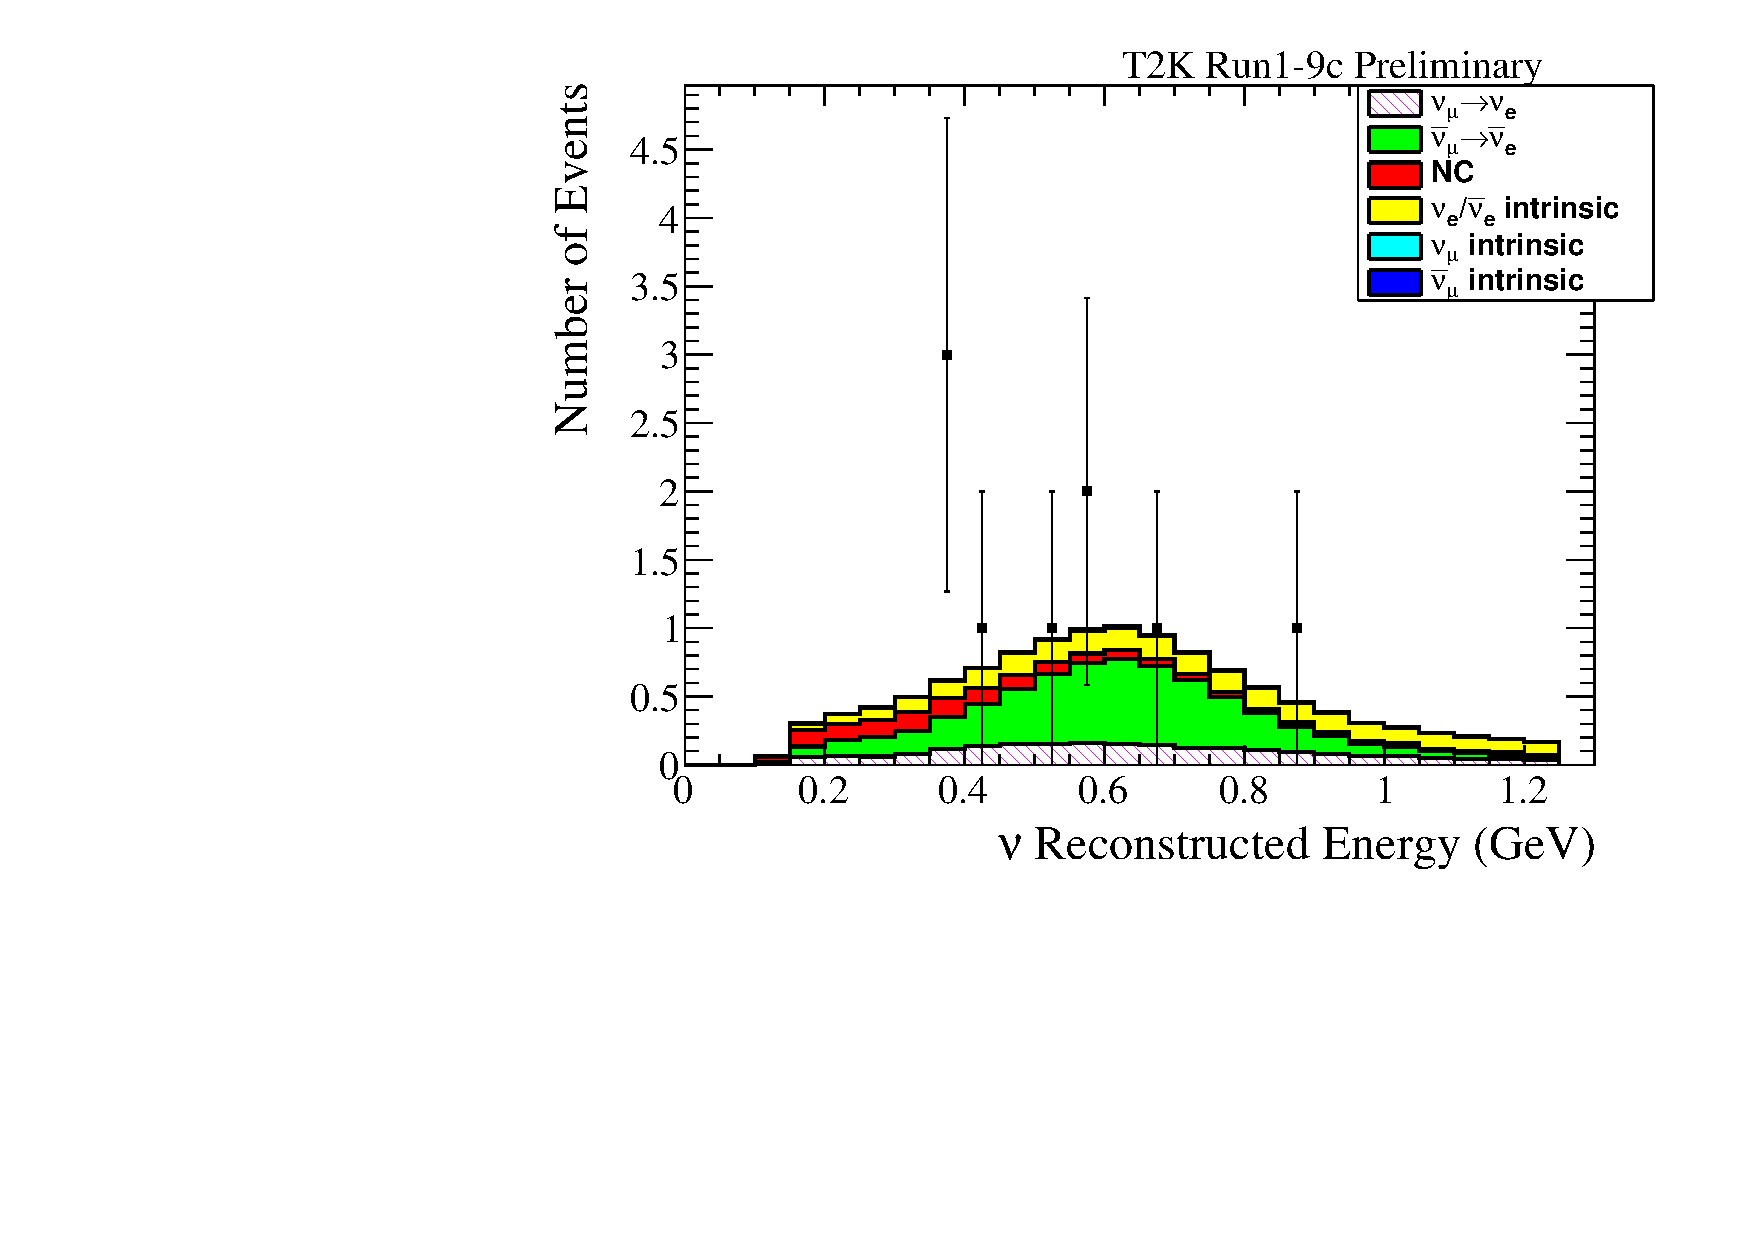
\includegraphics[width=0.9\textwidth]{images/spectra/data/erec_spectrum_asimov2018_RHC1Re_data}
		\caption{Electron-like antineutrino mode}
	\end{subfigure}
	\begin{subfigure}[b]{0.49\textwidth}
		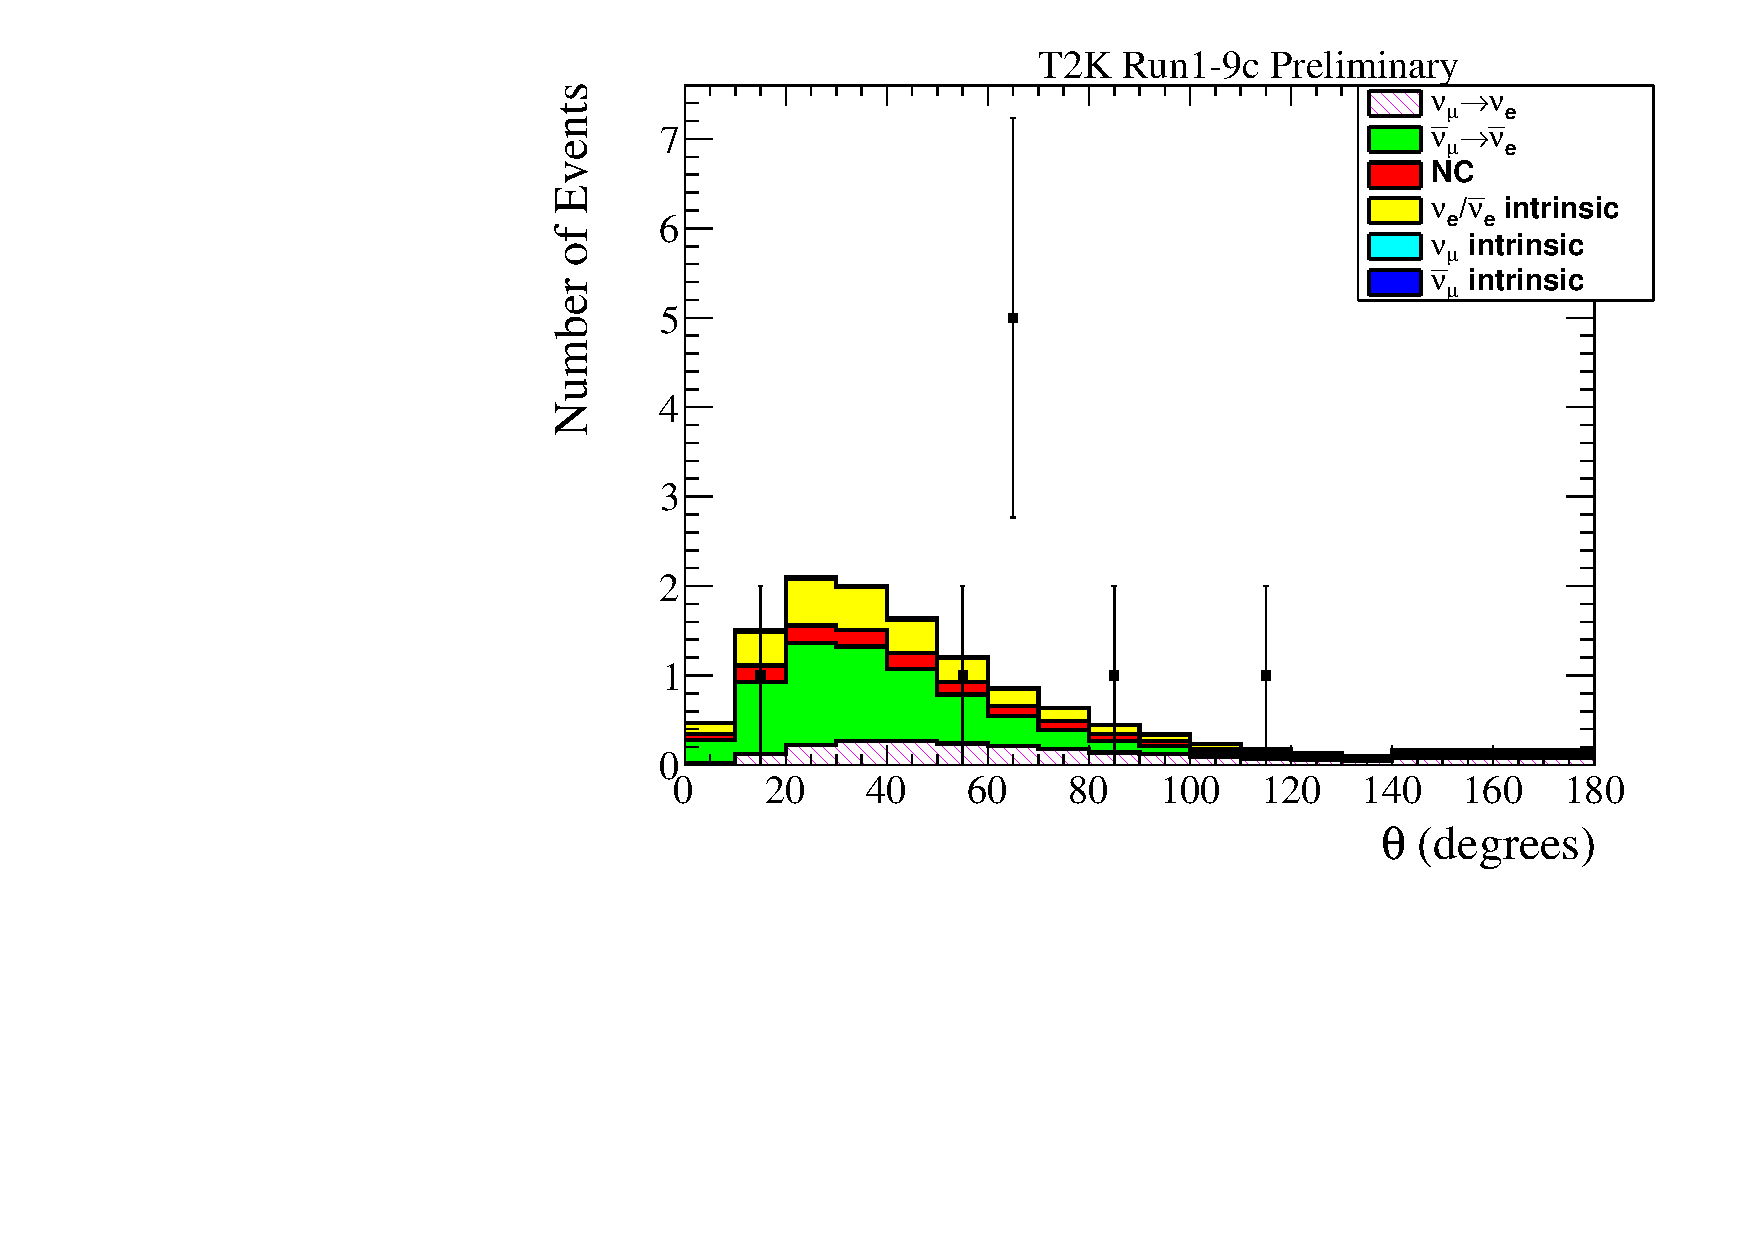
\includegraphics[width=0.9\textwidth]{images/spectra/data/theta_spectrum_asimov2018_RHC1Re_data}
		\caption{Electron-like antineutrino mode}
	\end{subfigure}

	\begin{subfigure}[b]{0.49\textwidth}
		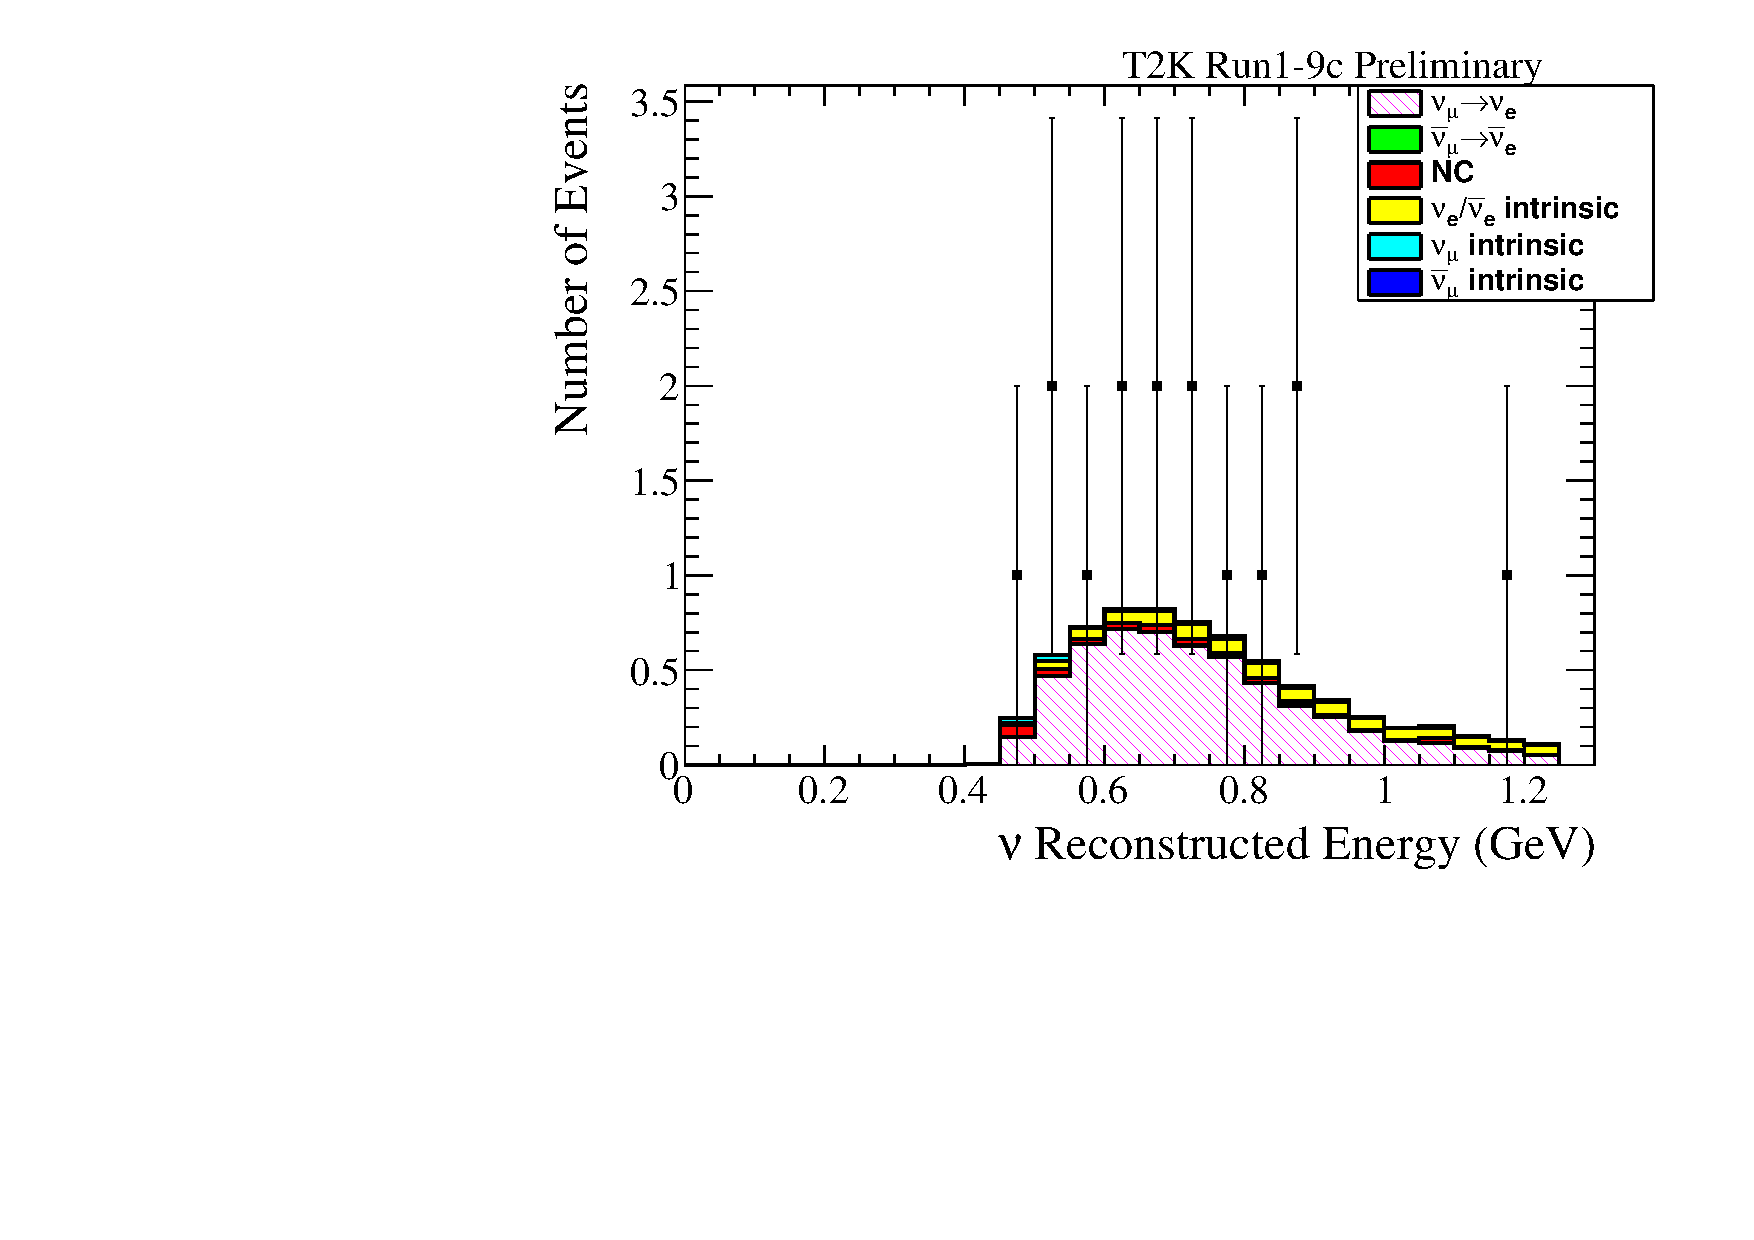
\includegraphics[width=0.9\textwidth]{images/spectra/data/erec_spectrum_asimov2018_MultiRe_data}
		\caption{\nueCConepi-like, neutrino mode}
	\end{subfigure}
	\begin{subfigure}[b]{0.49\textwidth}
		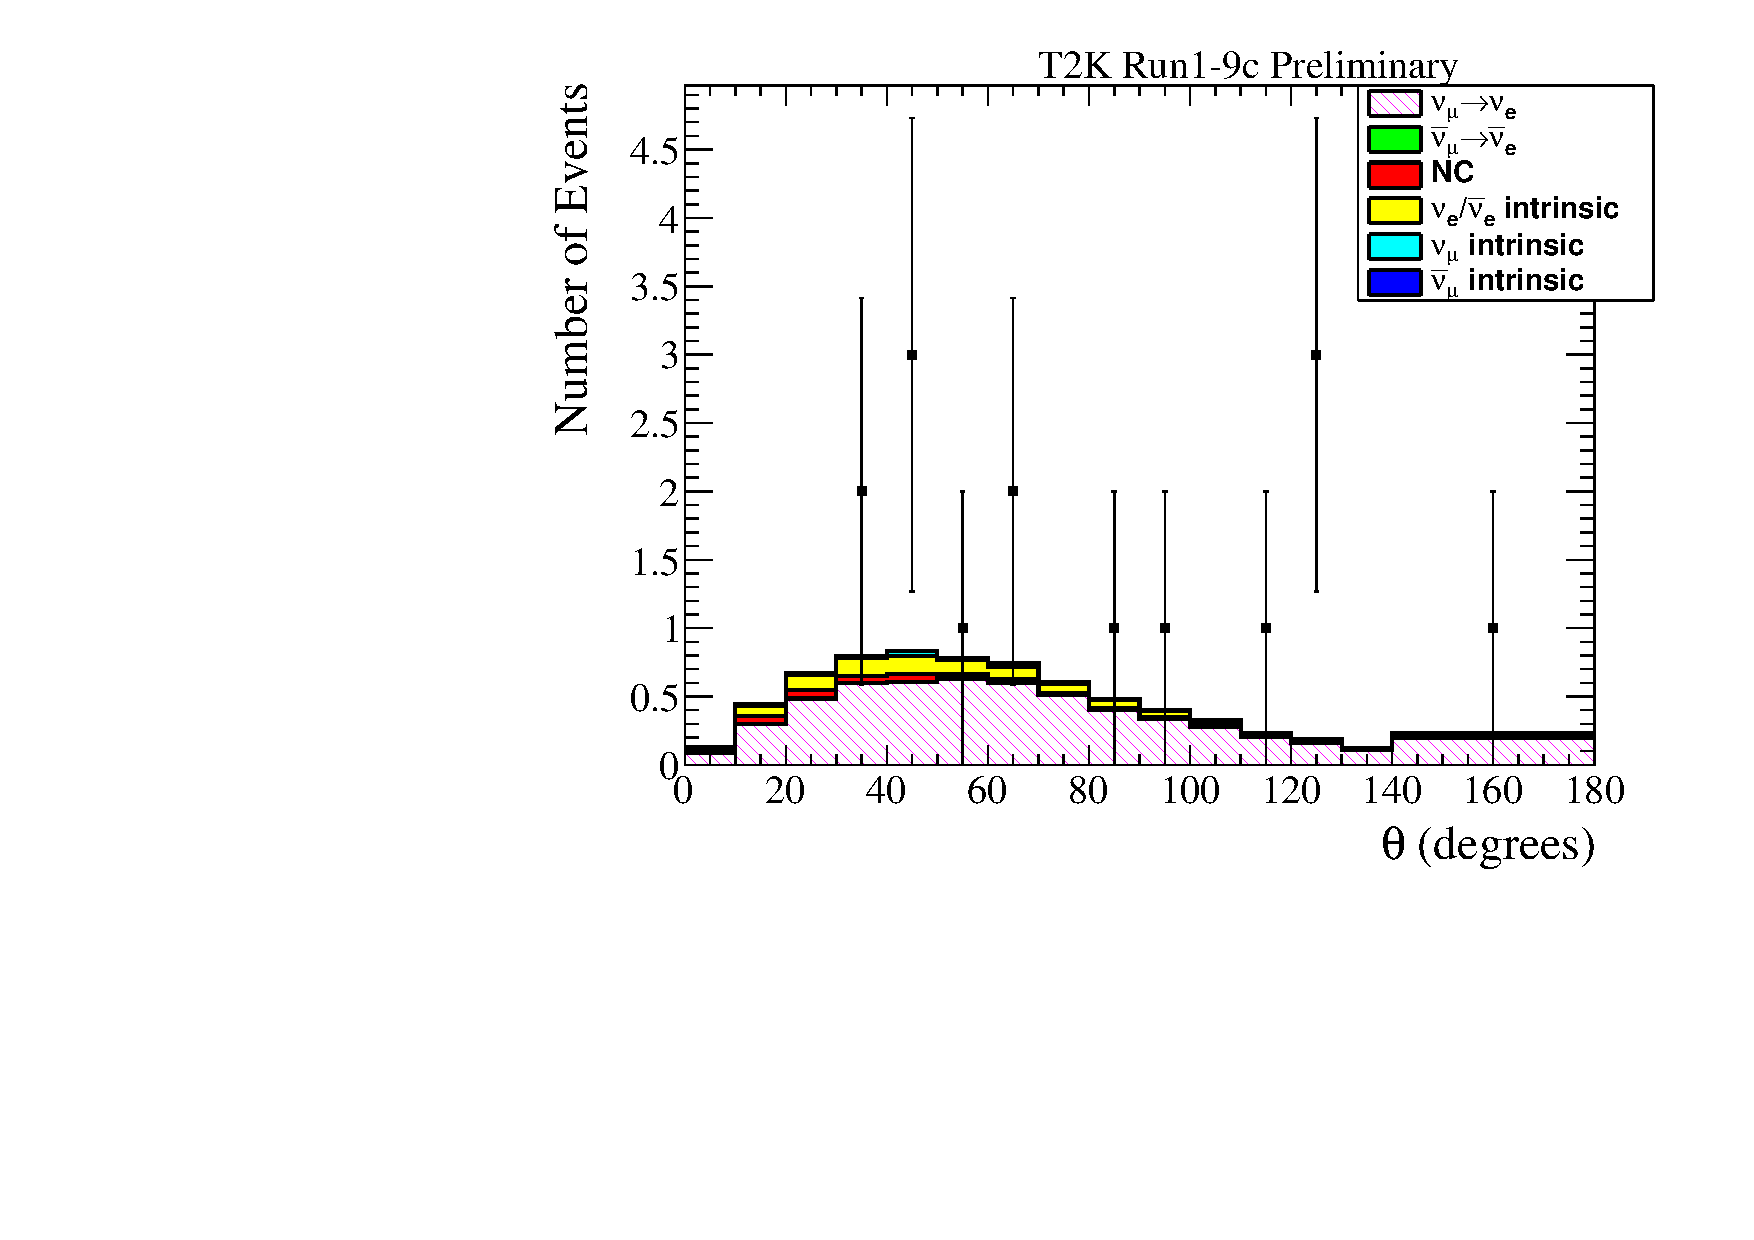
\includegraphics[width=0.9\textwidth]{images/spectra/data/theta_spectrum_asimov2018_MultiRe_data}
		\caption{\nueCConepi-like, neutrino mode}
	\end{subfigure}
	\caption {
		Predicted spectra and observed events (points). The $e$-like, including \nueCConepi, distributions are functions of both the reconstructed neutrino energy and the reconstructed angle between the outgoing lepton and the neutrino direction, with the projections in each variable shown here. The distributions correspond to the statistics collected in the full \RunPeriod data set. The spectra are generated with the systematic parameters described in \cref{sec:systematics} and the oscillation parameters corresponding to the best-fit values from the data fit (solar parameters at PDG 2016).
	}
	\label{fig:asimovpf_spectra_mc_data_elike_1D}
\end{figure*}
\clearpage

The best-fit values and $1\sigma$ ranges for each oscillation parameter are shown in \cref{tab:data_bestfit} for normal hierarchy (which is preferred in all data fits) and inverted hierarchy (local interval). The $1\sigma$ ranges are extracted for each oscillation parameter from the 1-dimensional $\Delta \chi^2$ distributions shown in \crefrange{fig:dcp_data}{fig:dmsq23_data}.

The 1-dimensional contours are plotted with respect to the global minimum from normal and inverted hierarchies, while the 2-dimensional confidence intervals are shown drawing the normal and inverted hierarchy contours independently, i.e. each contour is produced with respect to the global minimum under that hierarchy hypothesis.

The reactor measurements are in agreement with the T2K data at $1\sigma$ level for \deltacp.

\begin{table}
\centering
\begin{tabular}{| c | c | c | c | c | c |}
\hline
Parameter & Reactor & Best-fit (NH) & $\pm1\sigma$ (NH) & Best-fit (IH) & $\pm1\sigma$ (IH) \\
\hline
\deltacp & Yes & \BestFitDeltacpwRC & [\MOneSigmaDeltacpwRC,\POneSigmaDeltacpwRC] & \BestFitDeltacpwRCIH & [\MOneSigmaDeltacpwRCIH,\POneSigmaDeltacpwRCIH] \\
\deltacp & No & \BestFitDeltacpwoRC & [\MOneSigmaDeltacpwoRC,\POneSigmaDeltacpwoRC] & \BestFitDeltacpwoRCIH & [\MOneSigmaDeltacpwoRCIH,\POneSigmaDeltacpwoRCIH] \\
\ssqthonethree & No & \BestFitMixingOneThreewoRC & [\MOneMixingOneThreewoRC,\POneMixingOneThreewoRC] & \BestFitMixingOneThreewoRCIH & [\MOneMixingOneThreewoRCIH,\POneMixingOneThreewoRCIH] \\
\ssqthtwothree & Yes & \BestFitMixingTwoThreewRC & [\MOneMixingTwoThreewRC,\POneMixingTwoThreewRC] & \BestFitMixingTwoThreewRCIH & [\MOneMixingTwoThreewRCIH,\POneMixingTwoThreewRCIH] \\
\dmsqtwothree or \dmsqonethree & Yes & \BestFitDmTwoThreewRC & [\MOneDmTwoThreewRC,\POneDmTwoThreewRC] & \BestFitDmTwoThreewRCIH & [\MOneDmTwoThreewRCIH,\POneDmTwoThreewRCIH] \\
 ($10^{-3}\text{ eV}^2\text{/c}^4$) & & & & & \\
\hline
\end{tabular}

\caption{
The \RunPeriod measured oscillation parameter best-fit and the $\pm 1\sigma$ intervals are shown for normal and inverted hierarchies with respect to the hierarchy best-fit. The $\pm 1\sigma$ interval is obtained by using the constant $\Delta \chi^2$ method. For each parameter normal hierarchy is the global best-fit.
}
\label{tab:data_bestfit}
\end{table}

\clearpage

\subsection{Results for \appearance}
In \cref{fig:ssqth13_vs_dcp_data} the result for \appearance with reactor constraint and T2K only is shown.

\begin{figure*}[htb]
	\center
	\begin{subfigure}[b]{0.49\textwidth}
		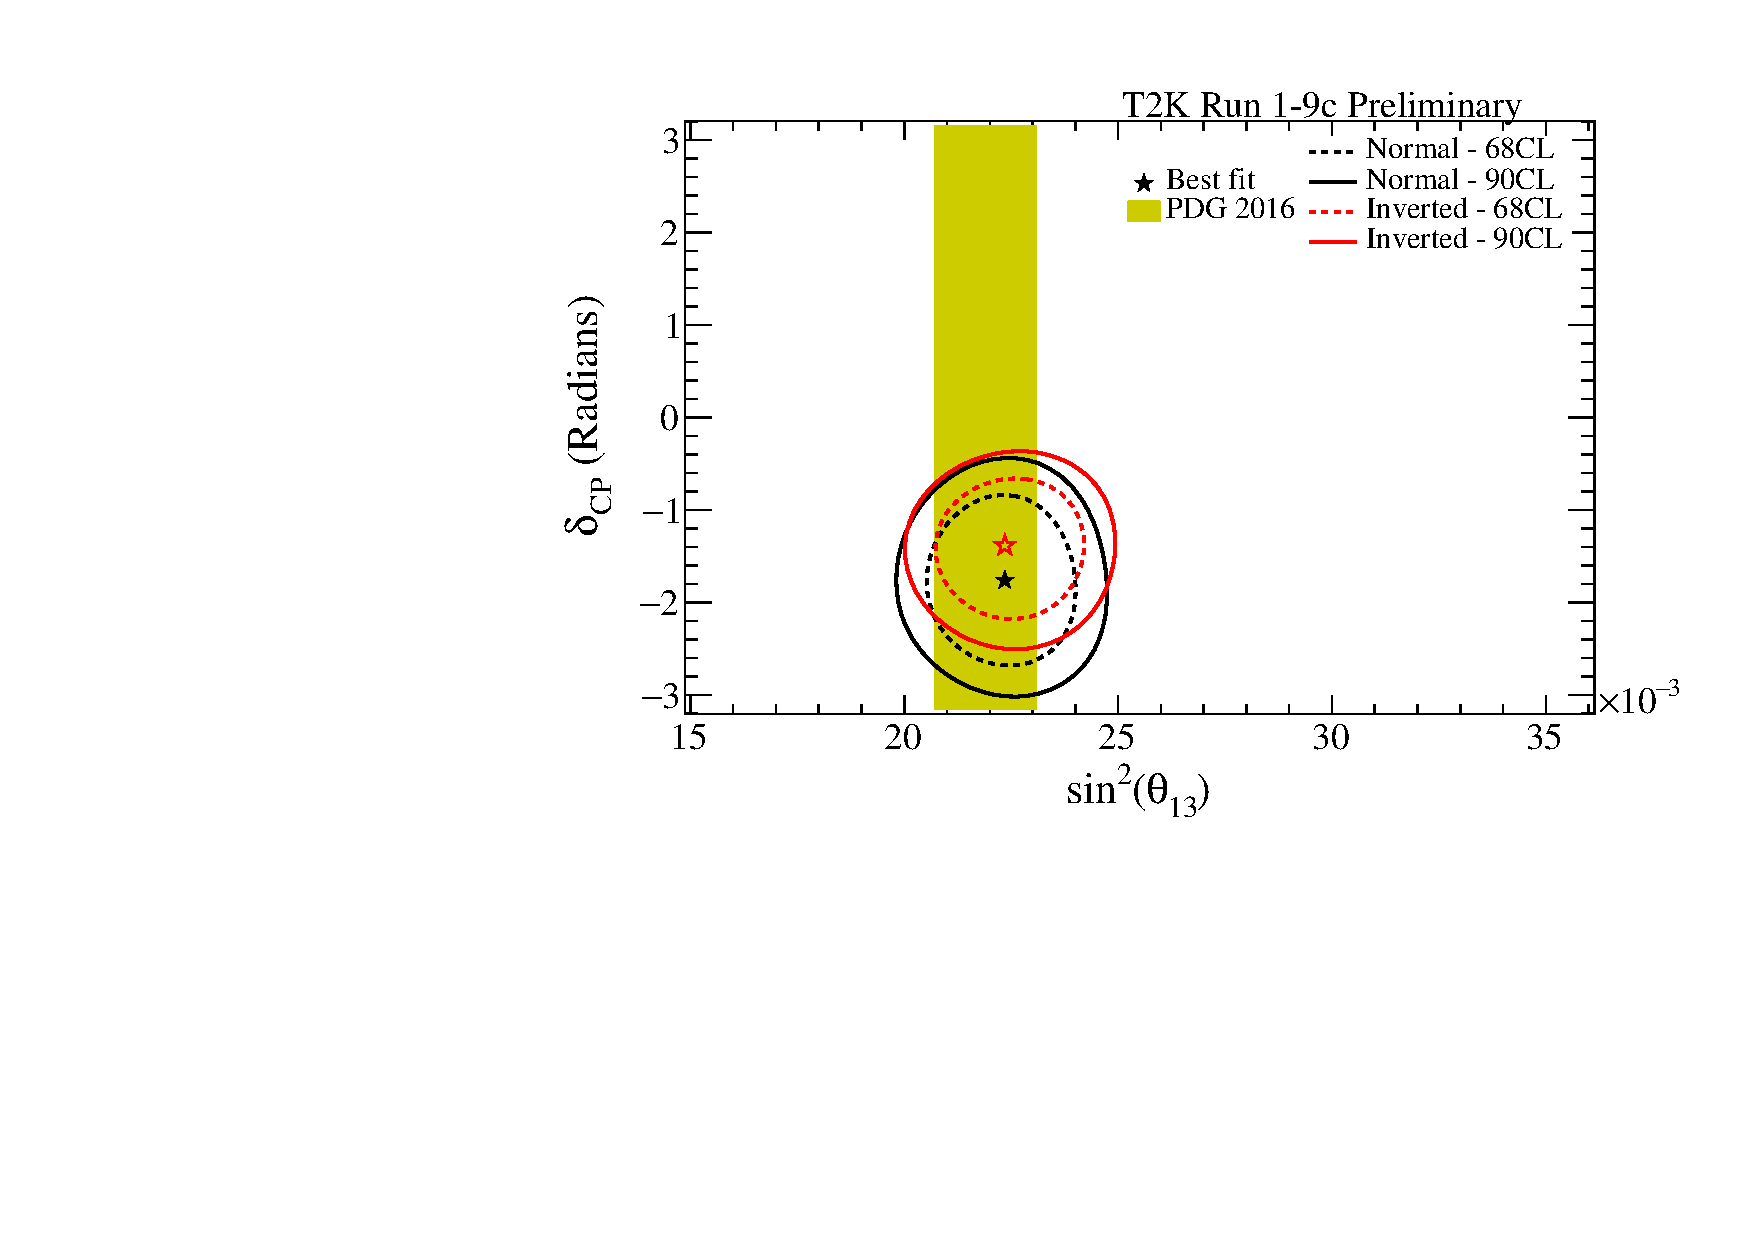
\includegraphics[width=0.9\textwidth]{images/data/mixing13_deltacp_data_reactor_global}
		\caption{\appearance with reactor constraint}
	\end{subfigure}
	\begin{subfigure}[b]{0.49\textwidth}
		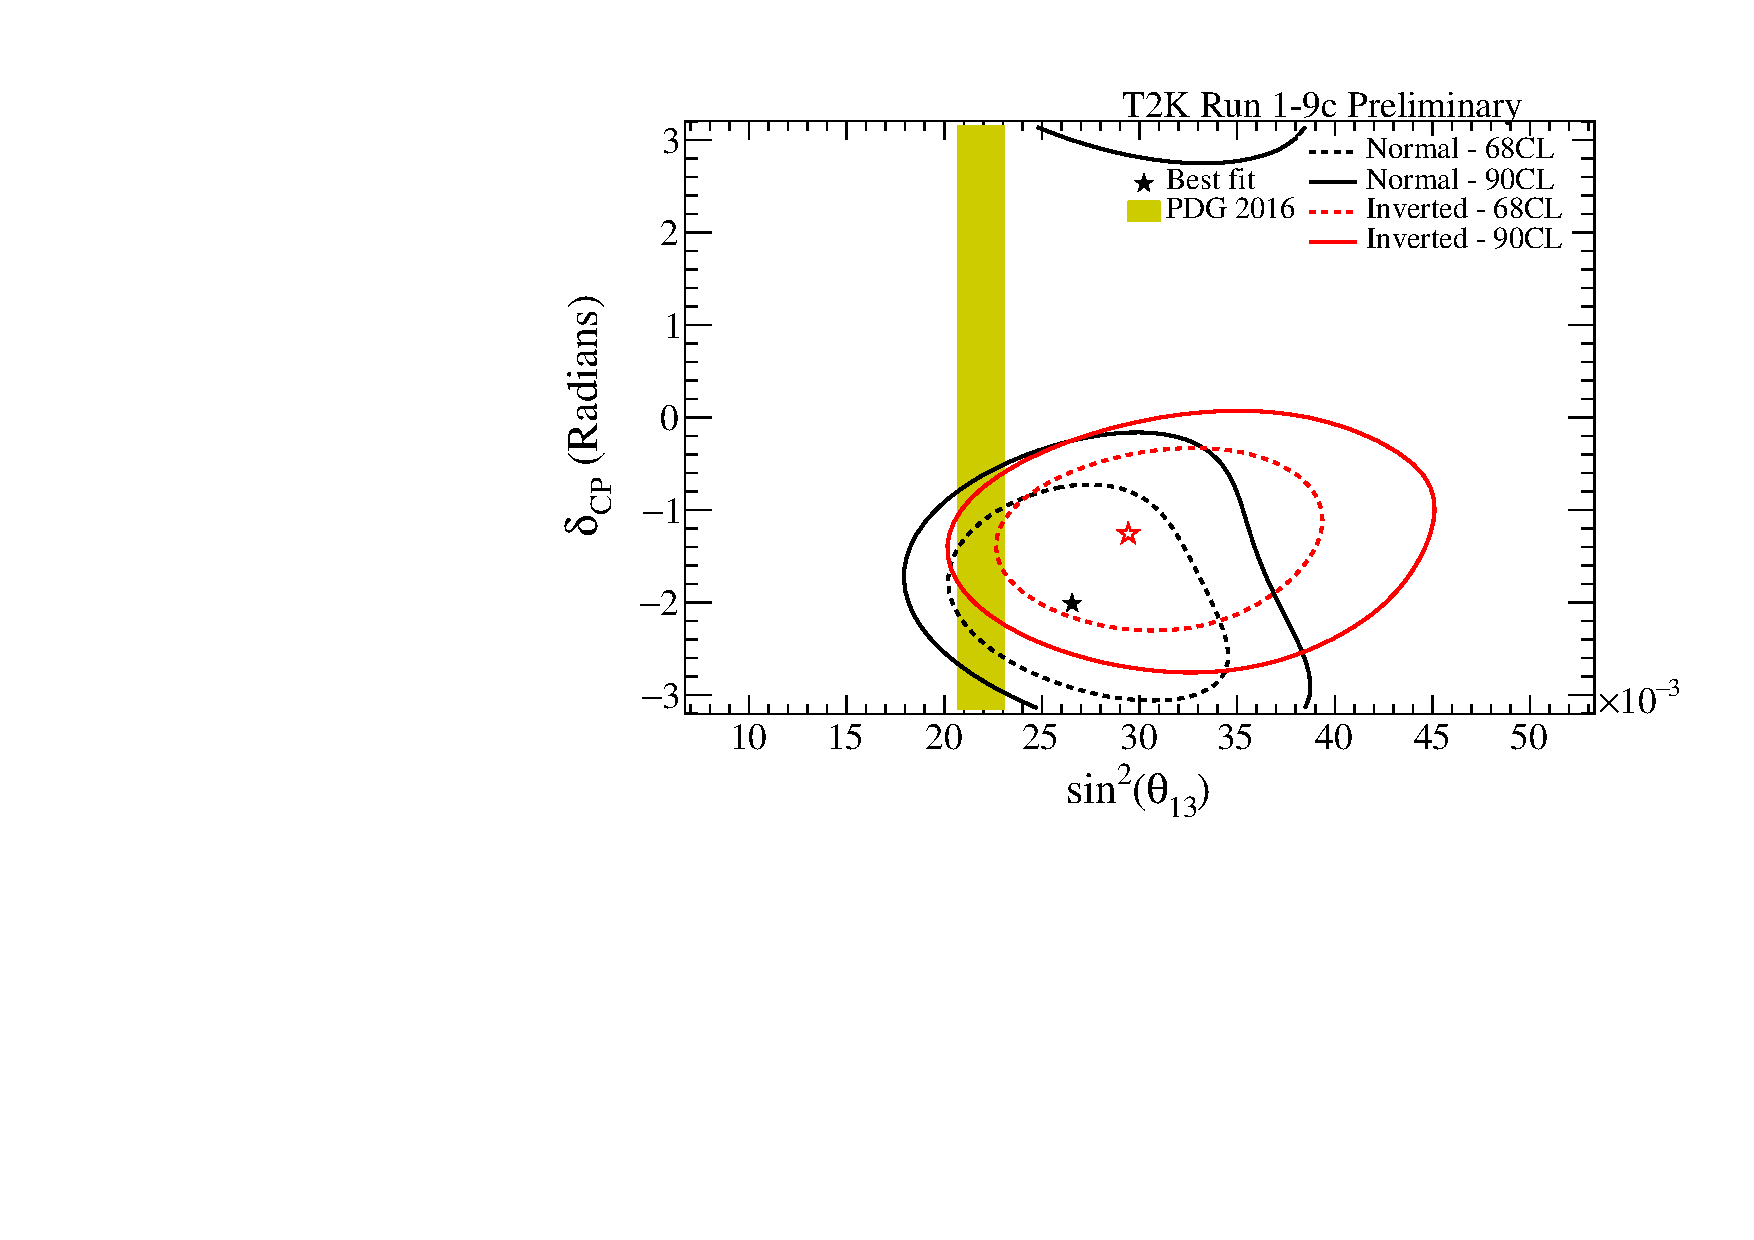
\includegraphics[width=0.9\textwidth]{images/data/mixing13_deltacp_data_t2k_global}
		\caption{\appearance T2K only}
	\end{subfigure}
	\caption {
		Contours at 68\% and 90\% CL for \appearance with and without reactor constraint. Normal and inverted hierarchy contours are independent. All 5 samples were used to produce these fits.
	}
	\label{fig:ssqth13_vs_dcp_data}
\end{figure*}

\subsection{Results for \disappearance}

The result for \disappearance with reactor constraint and T2K only is shown in fig.~\ref{fig:ssqth23_vs_dmsq23_data}.

\begin{figure*}[htb]
	\center
	\begin{subfigure}[b]{0.49\textwidth}
		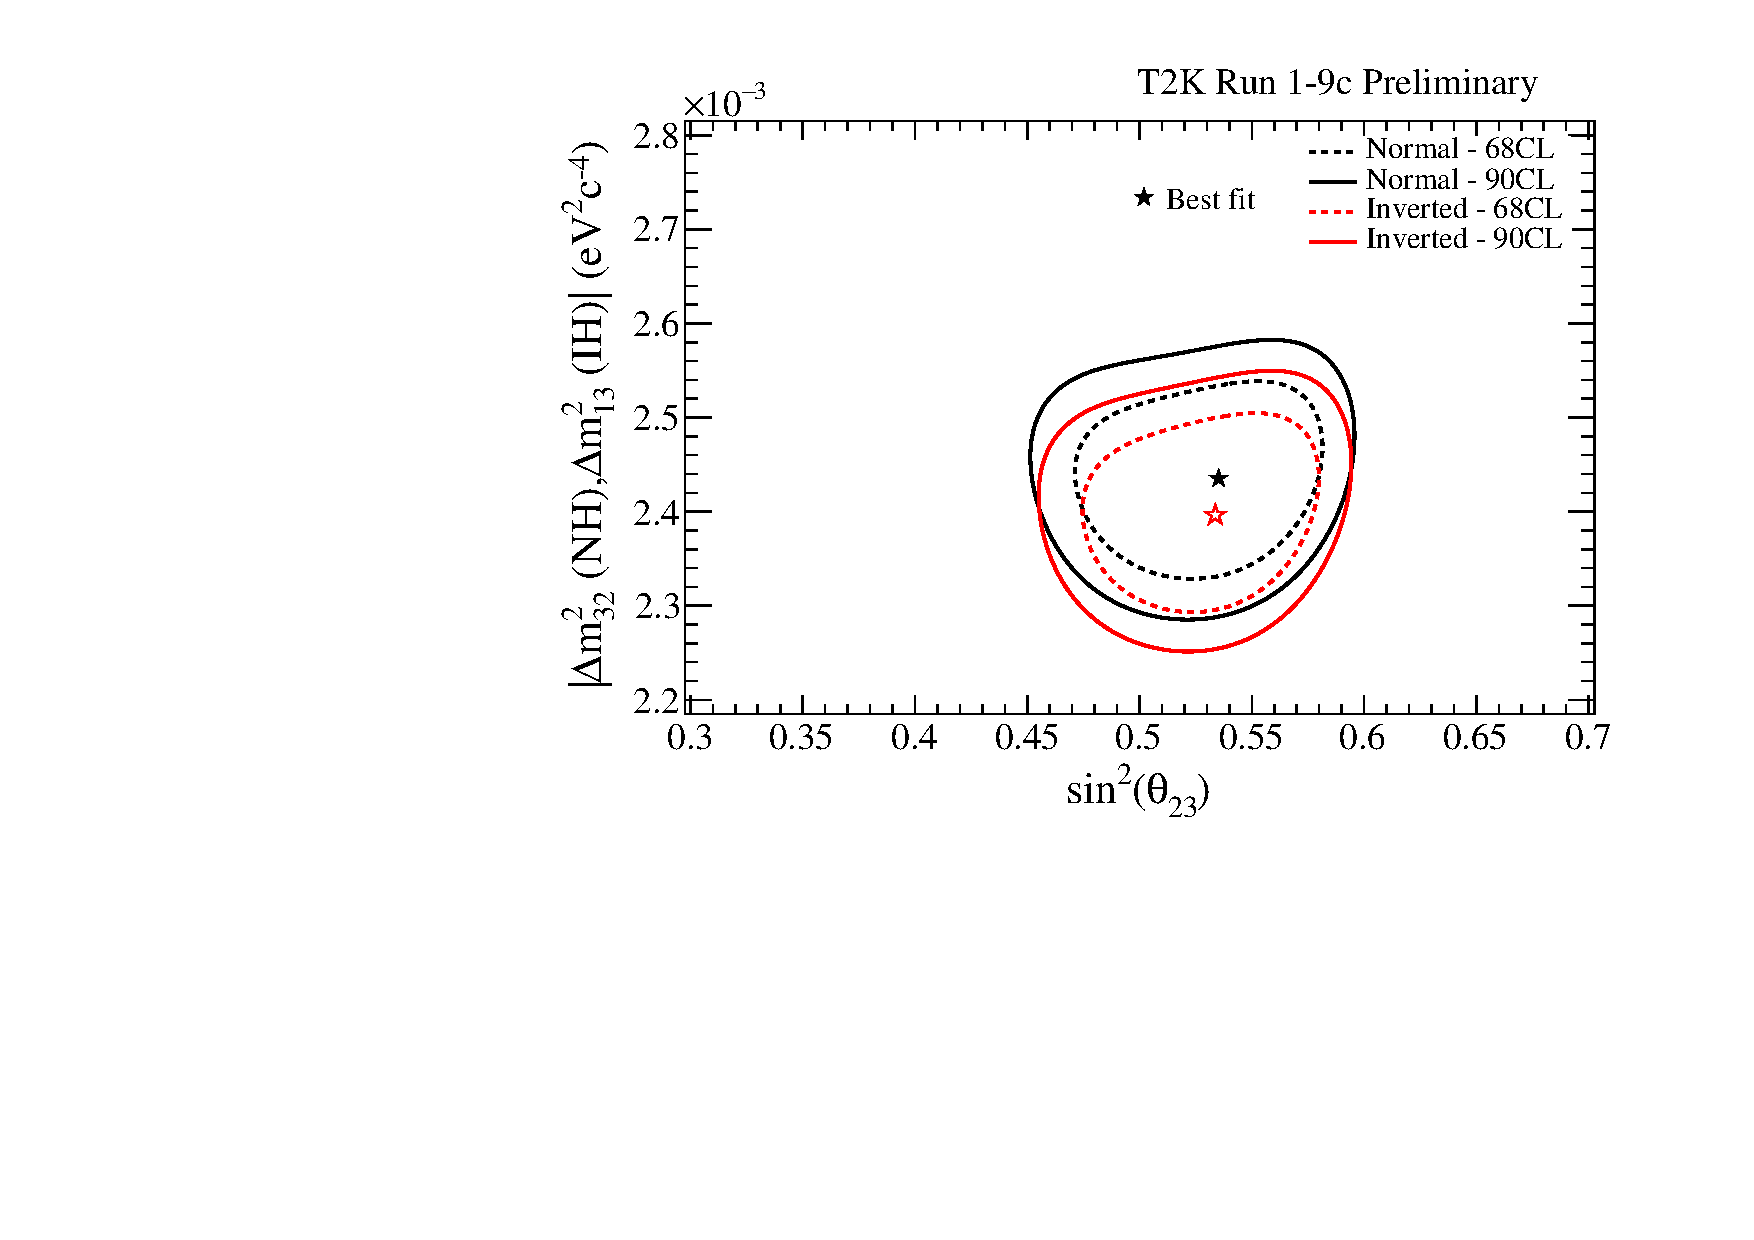
\includegraphics[width=0.9\textwidth]{images/data/mixing23_dmsq23_data_reactor_global}
		\caption{\disappearance with reactor constraint}
	\end{subfigure}
	\begin{subfigure}[b]{0.49\textwidth}
		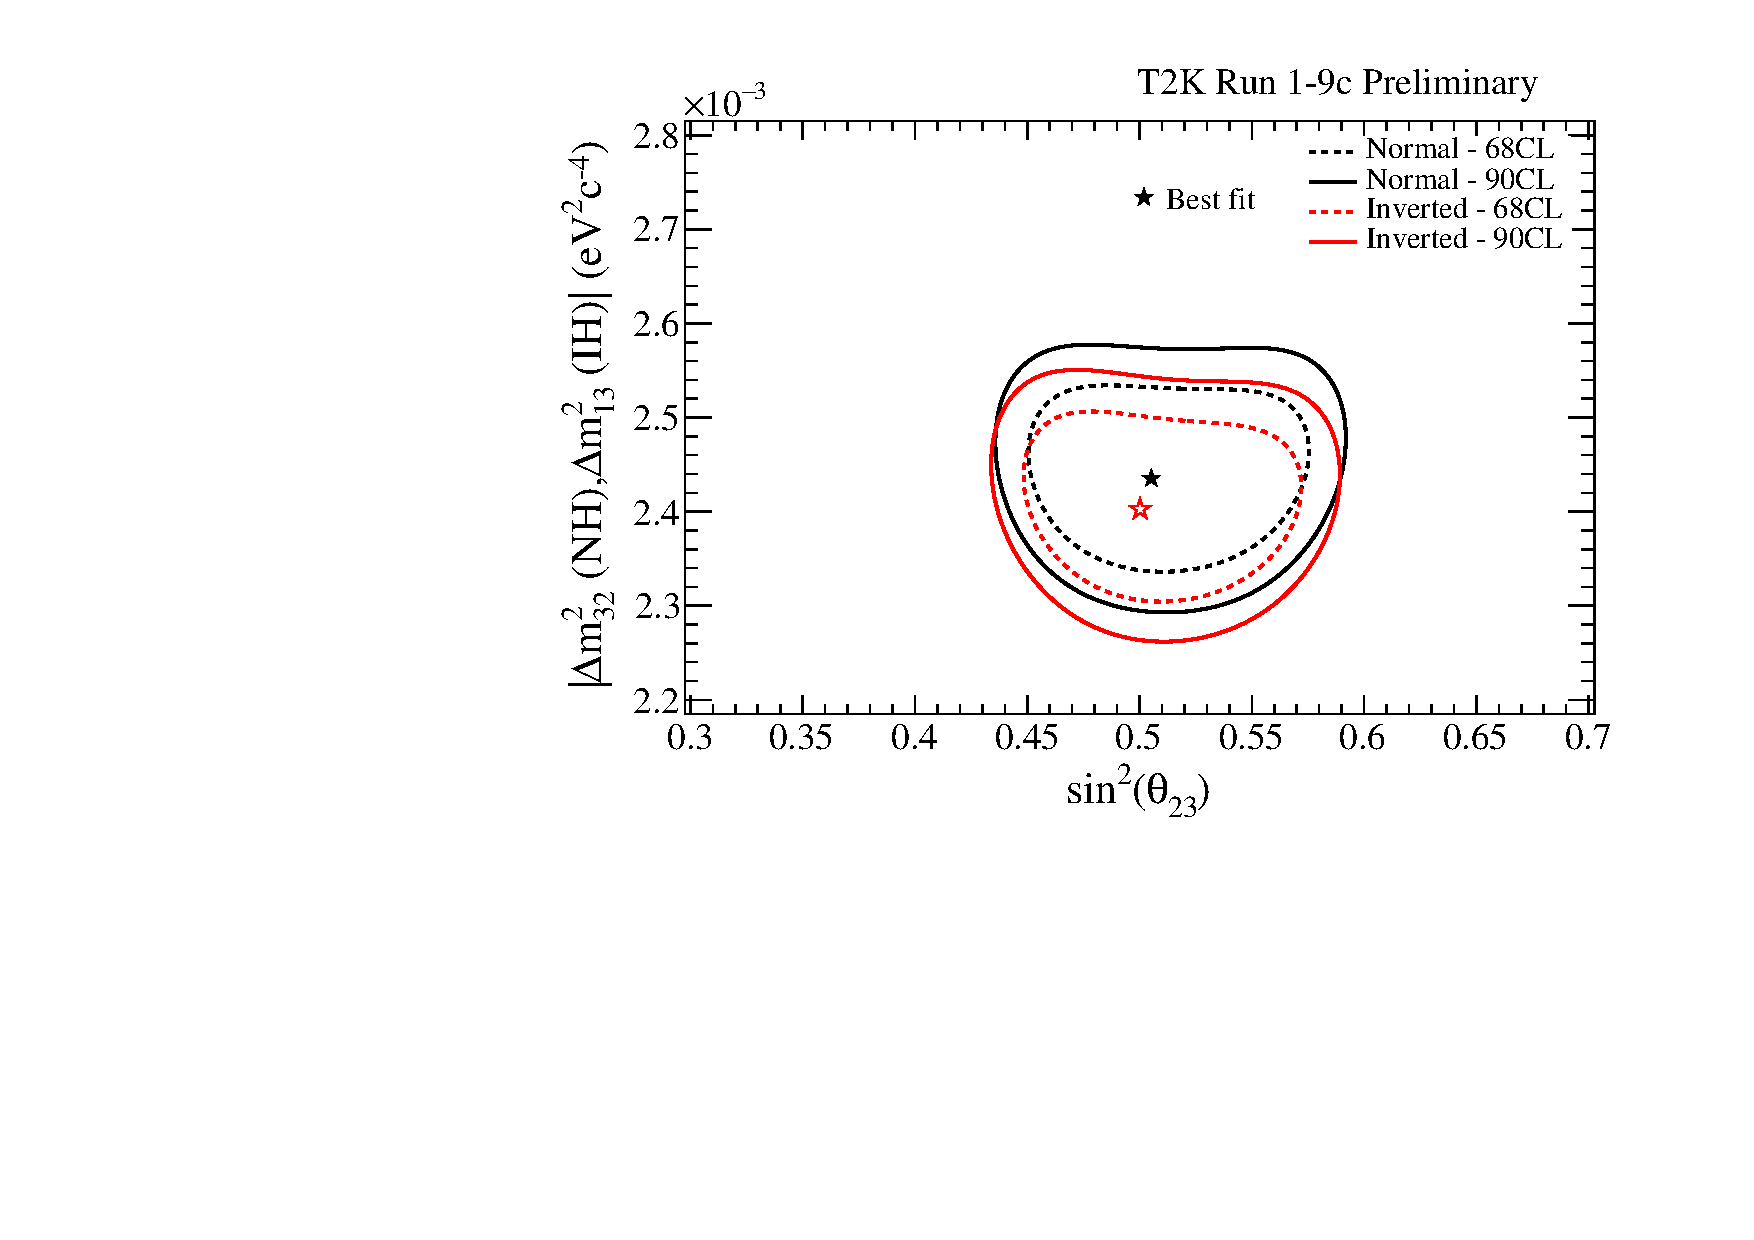
\includegraphics[width=0.9\textwidth]{images/data/mixing23_dmsq23_data_t2k_global}
		\caption{\disappearance T2K only}
	\end{subfigure}
	\caption {
		Contours at 68\% and 90\% CL for \disappearance with and without reactor constraint. Normal and inverted hierarchy contours are independent. All 5 samples were used to produce these fits.
	}
	\label{fig:ssqth23_vs_dmsq23_data}
\end{figure*}

\clearpage

\subsection{Results for \deltacp}

The result for \deltacp with reactor constraint and T2K only is shown in fig.~\ref{fig:dcp_data}.

\begin{figure*}[htb]
	\center
	\begin{subfigure}[b]{0.49\textwidth}
		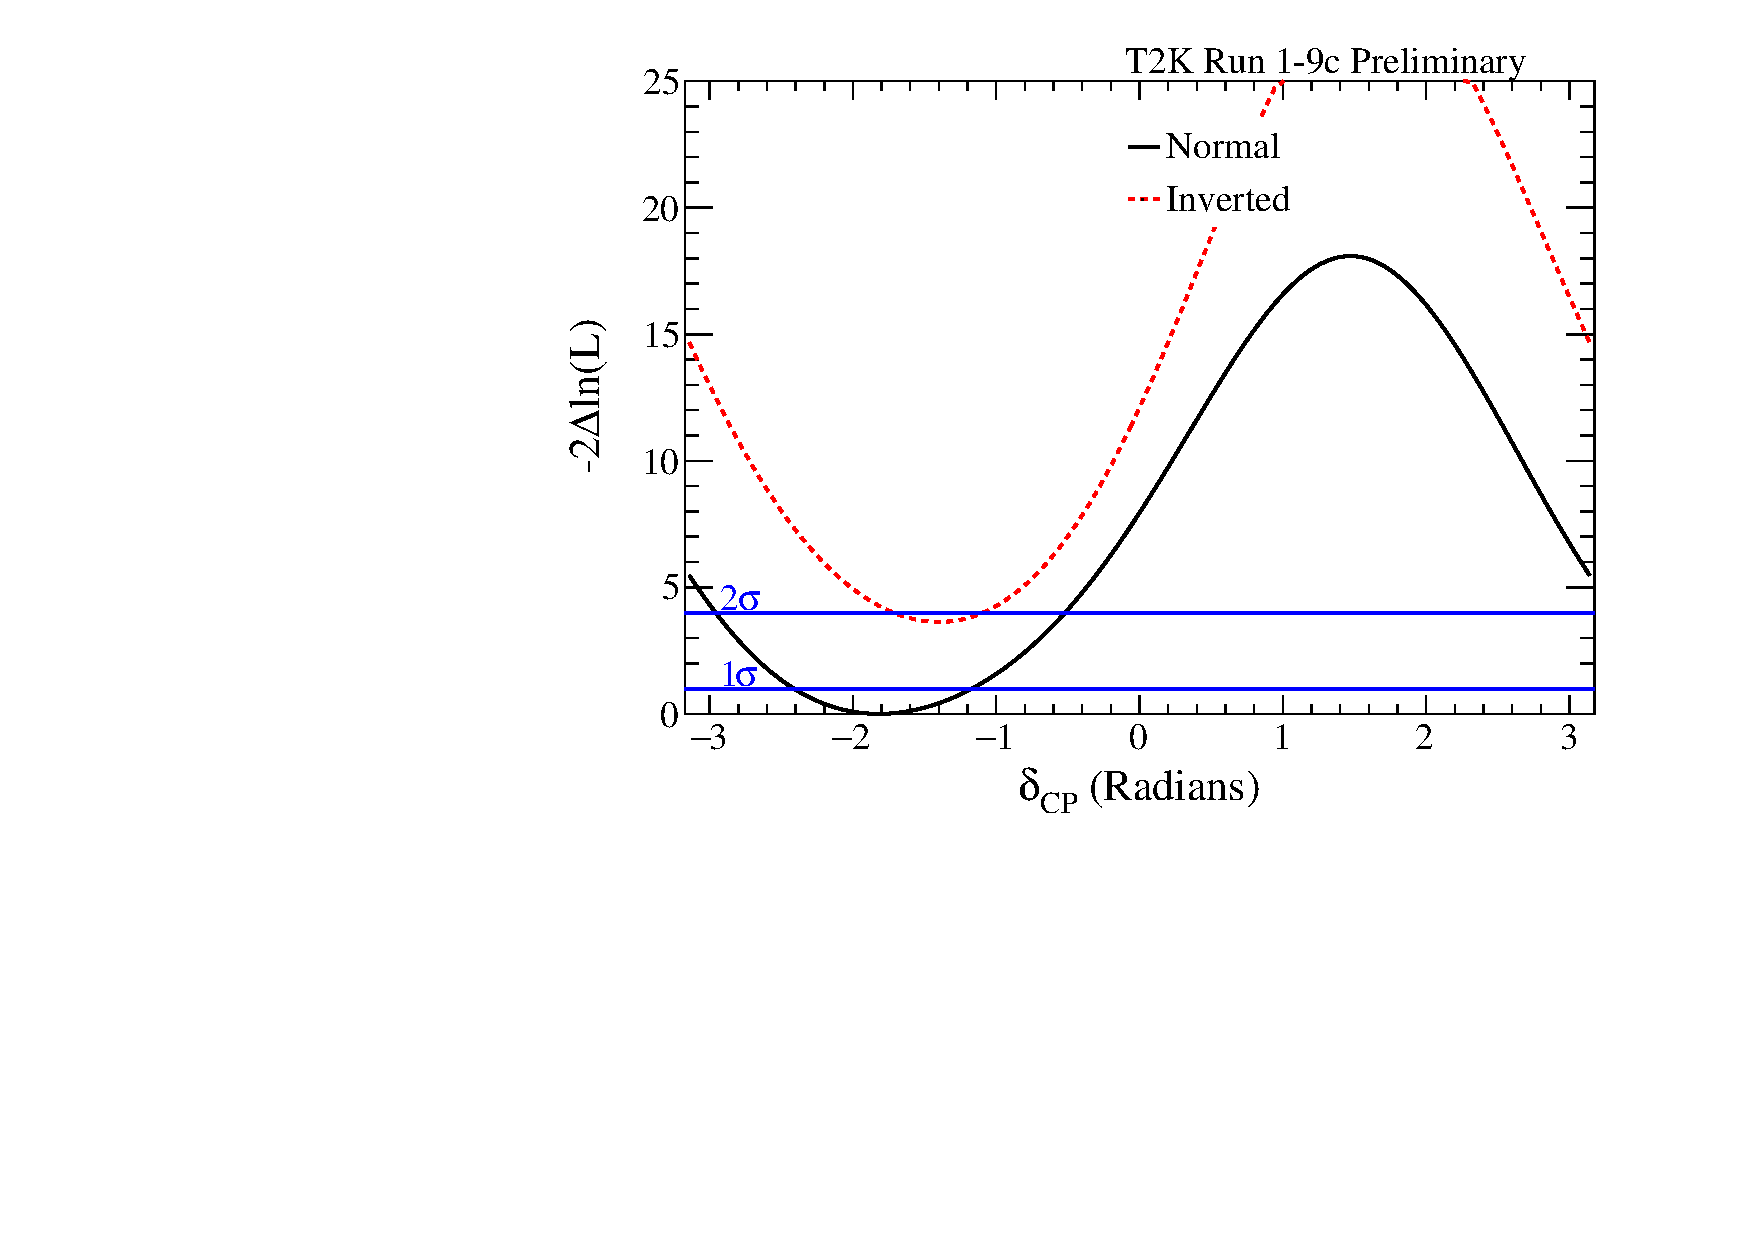
\includegraphics[width=0.9\textwidth]{images/data/deltacp_data_reactor_global}
		\caption{\deltacp with reactor constraint}
	\end{subfigure}
	\begin{subfigure}[b]{0.49\textwidth}
		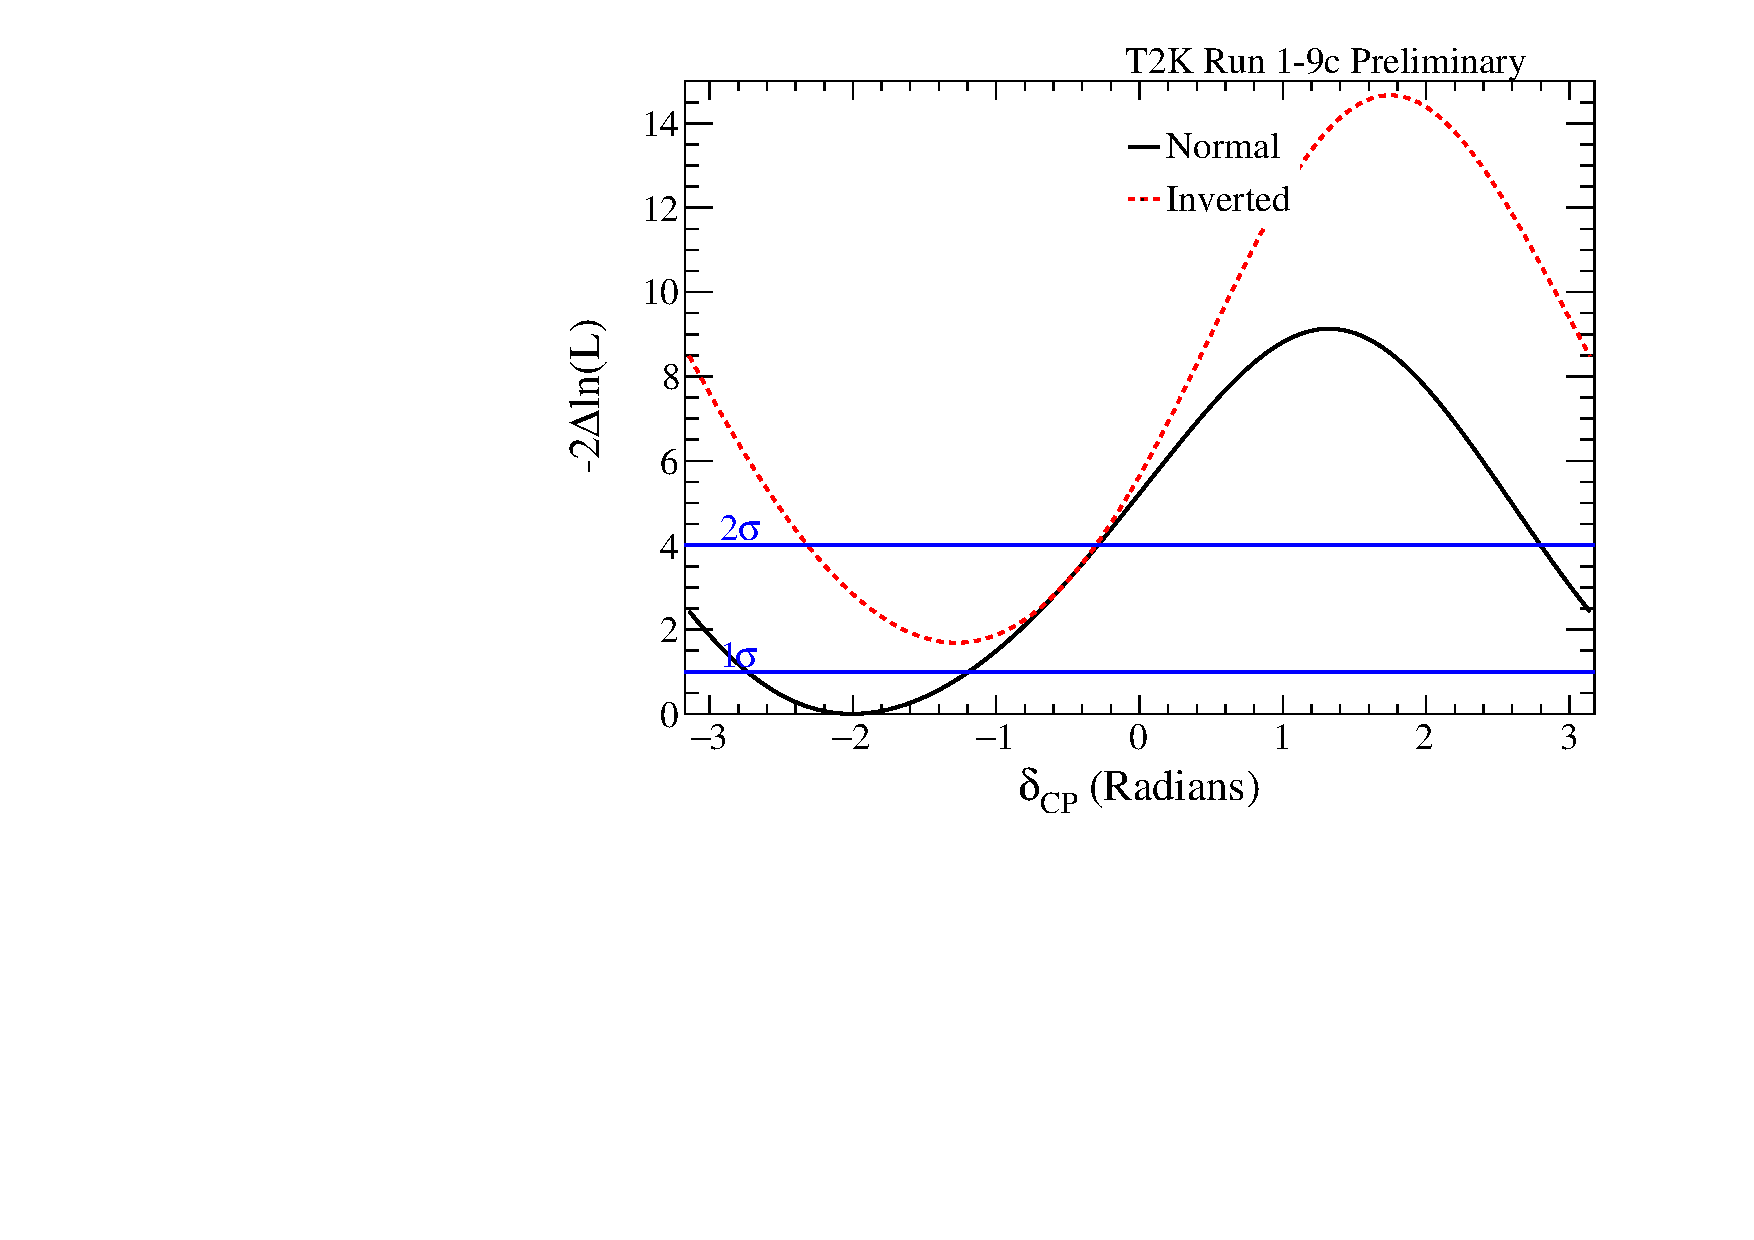
\includegraphics[width=0.9\textwidth]{images/data/deltacp_data_t2k_global}
		\caption{\deltacp T2K only}
	\end{subfigure}
	\caption {
		The expected $\Delta\chi^2$ distribution as a function of \deltacp with and without reactor constraint. The mass hierarchy is minimized, with normal and inverted hierarchy $\Delta\chi^2$ distributions shifted to the same global best-fit $\chi^2$ value, which is taken to be the minimum between normal and inverted hierarchy. All 5 samples were used to produce these fits.
	}
	\label{fig:dcp_data}
\end{figure*}

\subsection{Results for \ssqthonethree}

The result for \ssqthonethree (without reactor constraint) is shown in fig.~\ref{fig:th13_data}.

\begin{figure*}[htb]
	\center
	\begin{subfigure}[b]{0.49\textwidth}
		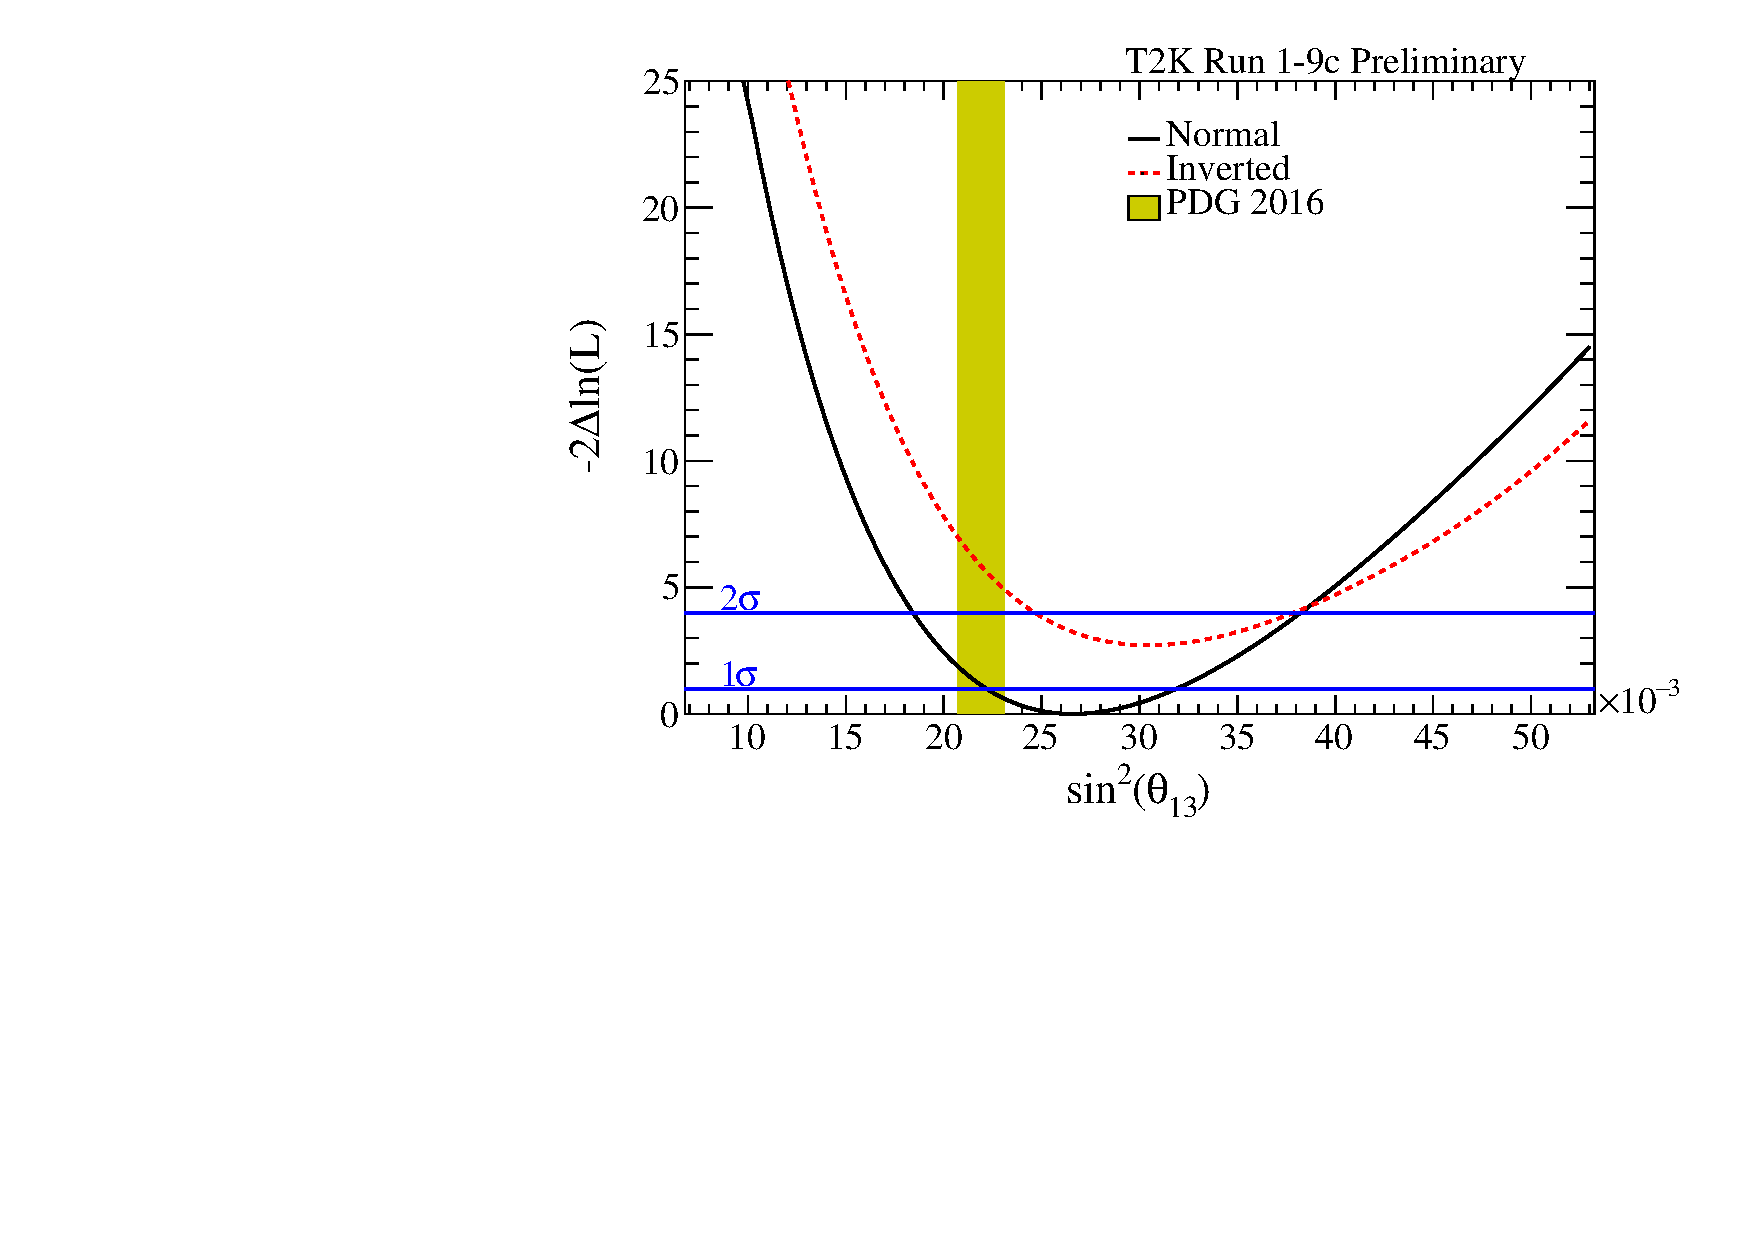
\includegraphics[width=0.9\textwidth]{images/data/mixing13_data_t2k_global}
		\caption{\ssqthonethree T2K only}
	\end{subfigure}
	\caption {
		The expected $\Delta\chi^2$ distribution as a function of \ssqthonethree without reactor constraint. The mass hierarchy is minimized, with normal and inverted hierarchy $\Delta\chi^2$ distributions shifted to the same global best-fit $\chi^2$ value, which is taken to be the minimum between normal and inverted hierarchy. All 5 samples were used to produce these fits.
	}
	\label{fig:th13_data}
\end{figure*}

\clearpage

\subsection{Results for \ssqthtwothree}

The result for \ssqthtwothree with reactor constraint and T2K only is shown in fig.~\ref{fig:th23_data}.

\begin{figure*}[htb]
	\center
	\begin{subfigure}[b]{0.49\textwidth}
		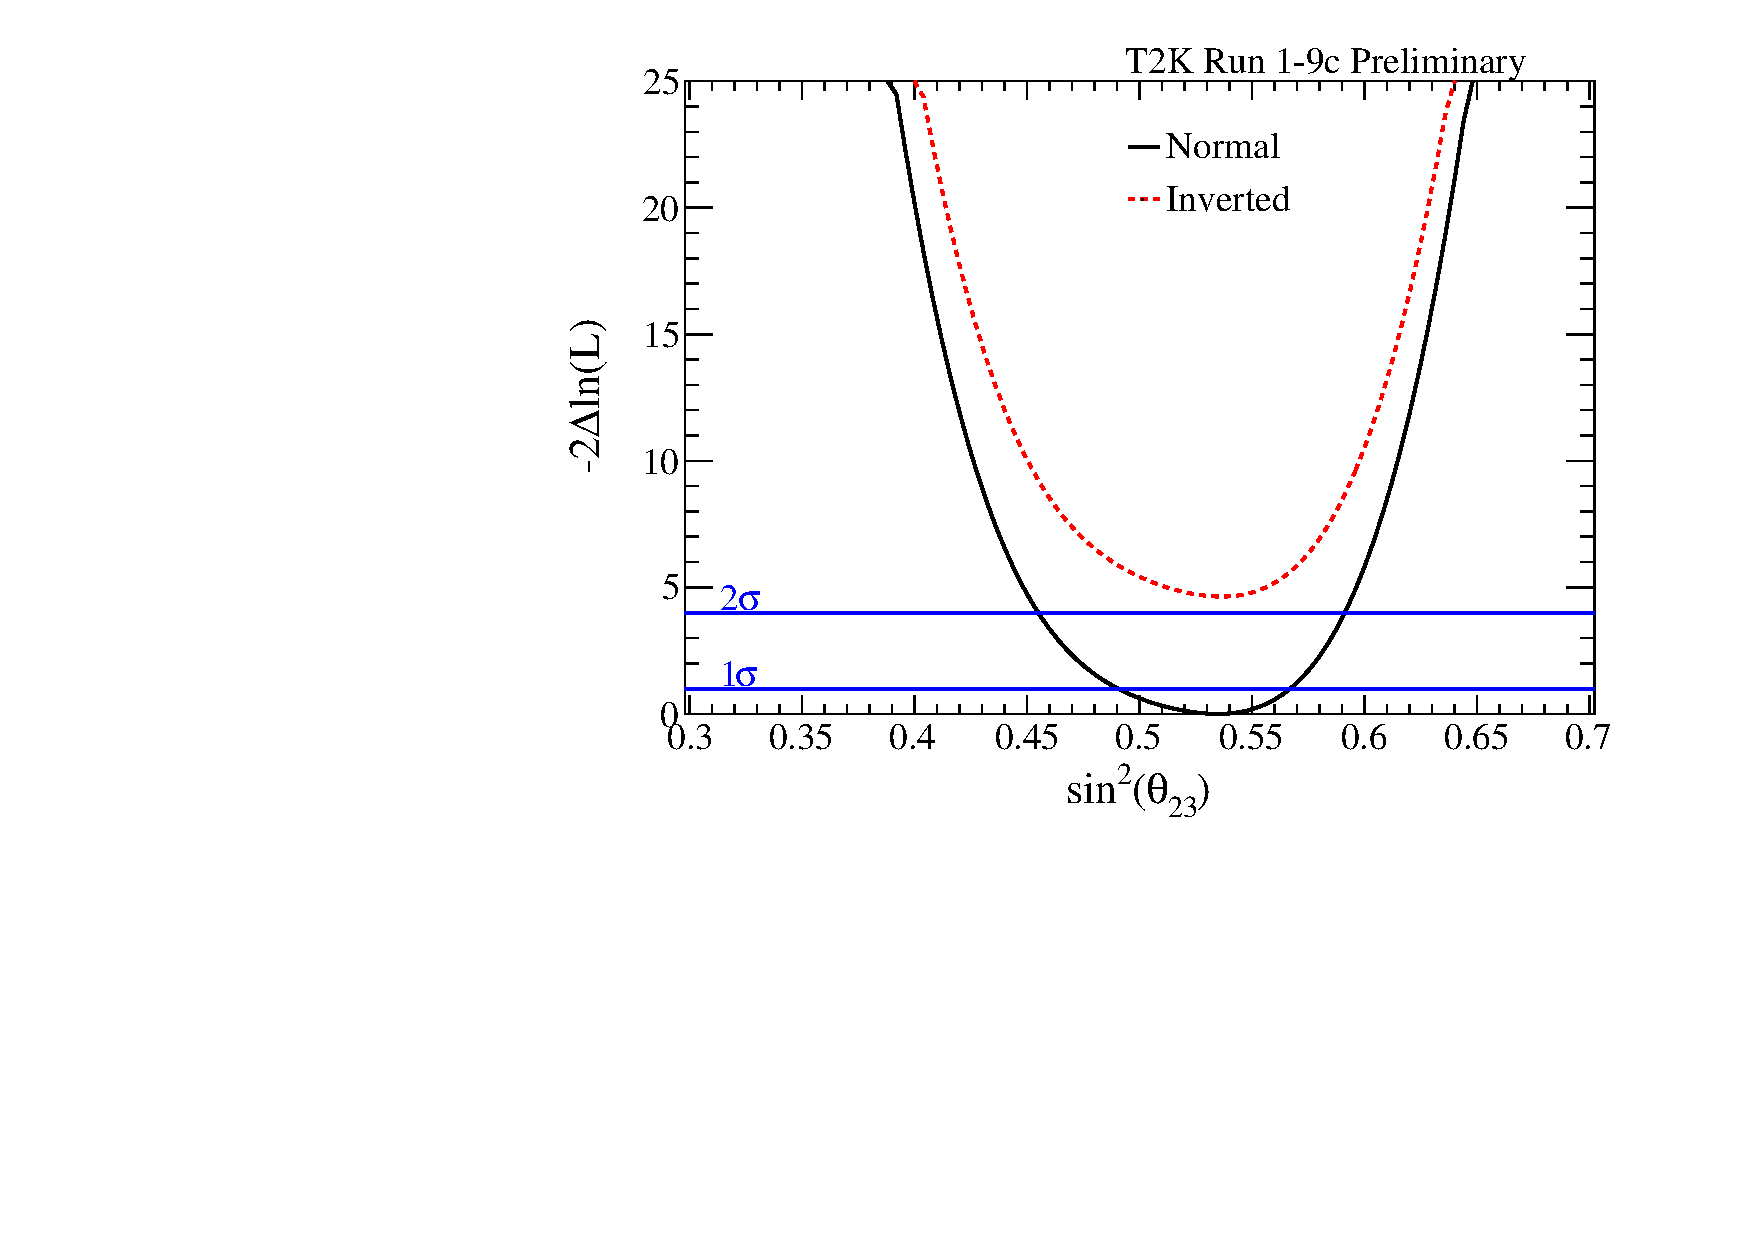
\includegraphics[width=0.9\textwidth]{images/data/mixing23_data_reactor_global}
		\caption{\ssqthtwothree with reactor constraint}
	\end{subfigure}
	\begin{subfigure}[b]{0.49\textwidth}
		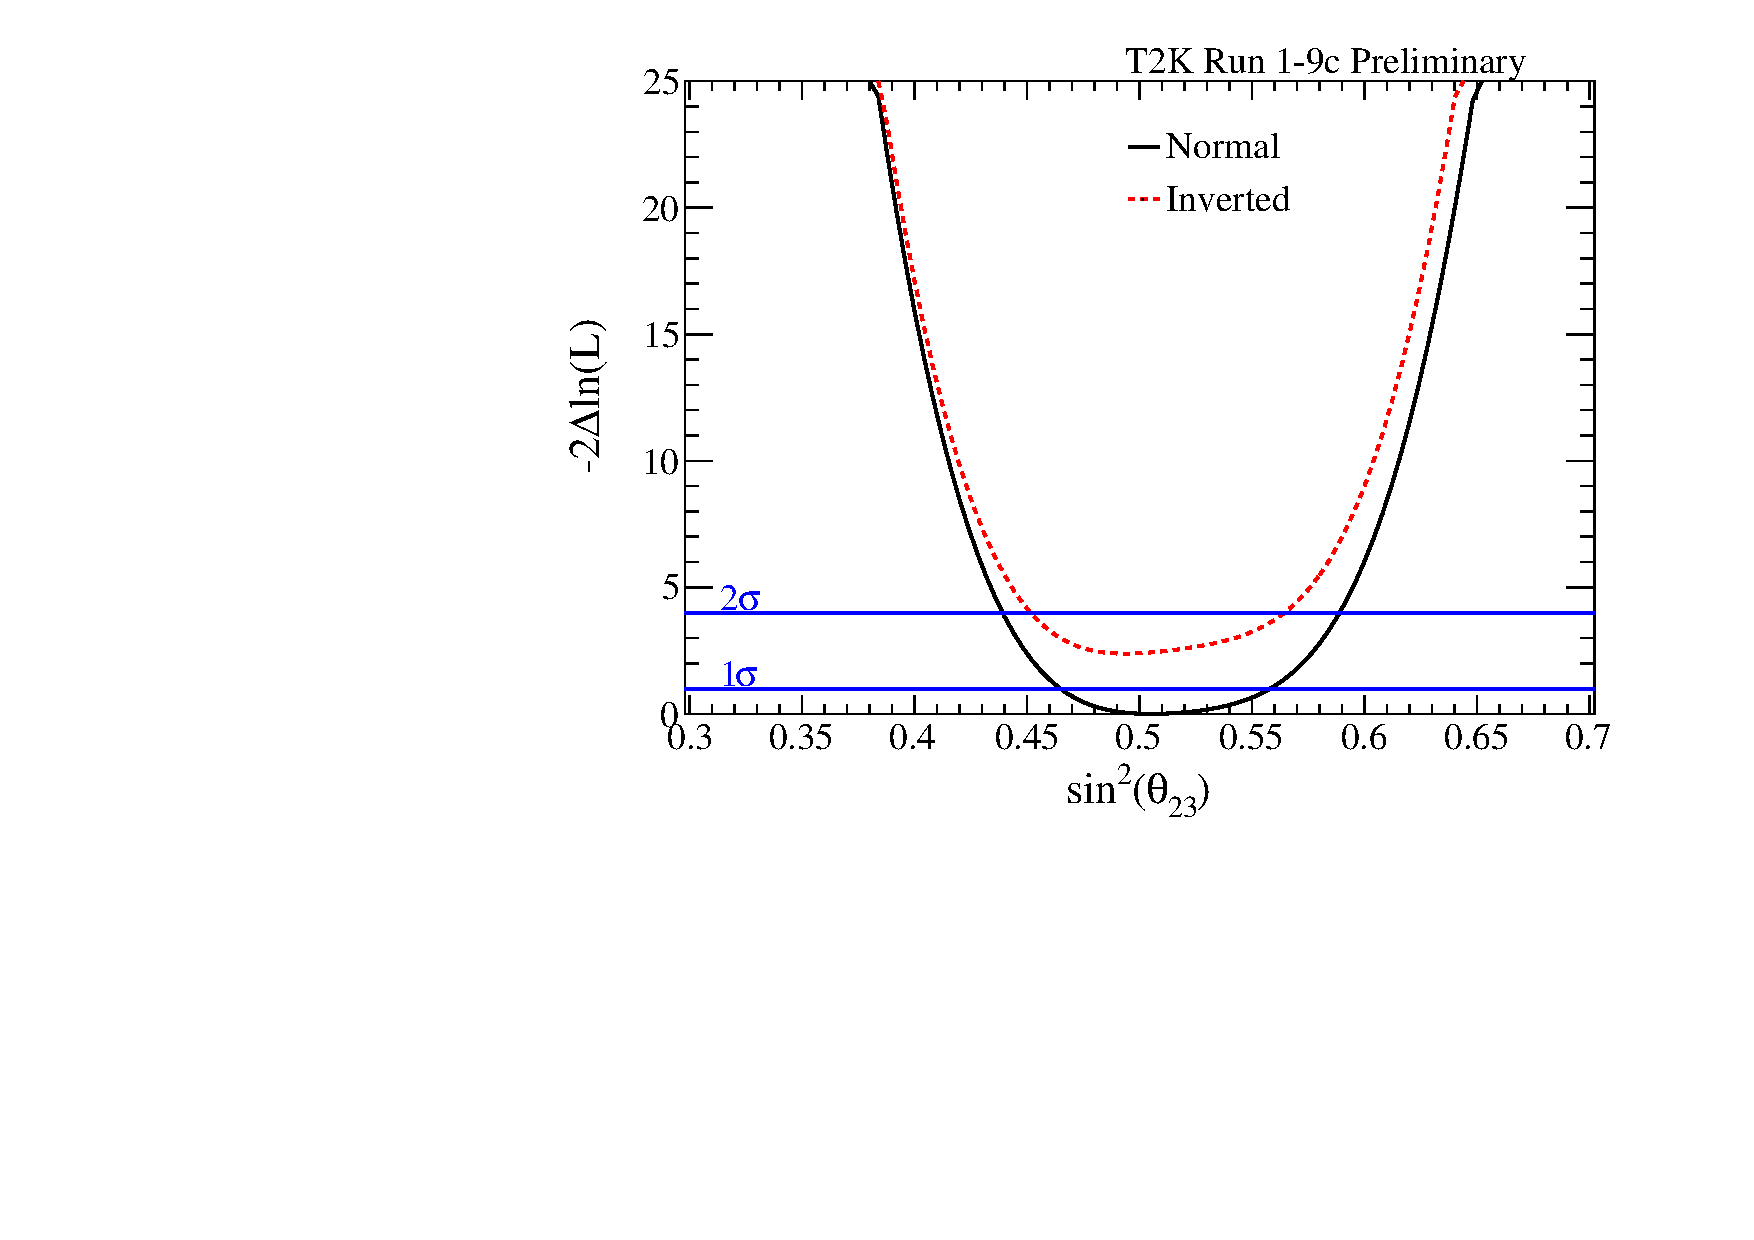
\includegraphics[width=0.9\textwidth]{images/data/mixing23_data_t2k_global}
		\caption{\ssqthtwothree T2K only}
	\end{subfigure}
	\caption {
		The expected $\Delta\chi^2$ distribution as a function of \ssqthtwothree with and without reactor constraint. The mass hierarchy is minimized, with normal and inverted hierarchy $\Delta\chi^2$ distributions shifted to the same global best-fit $\chi^2$ value, which is taken to be the minimum between normal and inverted hierarchy. All 5 samples were used to produce these fits.
	}
	\label{fig:th23_data}
\end{figure*}

\subsection{Results for \dmsq}

The result for \dmsq with reactor constraint and T2K only is shown in fig.~\ref{fig:dmsq23_data}.

\begin{figure*}[htb]
	\center
	\begin{subfigure}[b]{0.49\textwidth}
		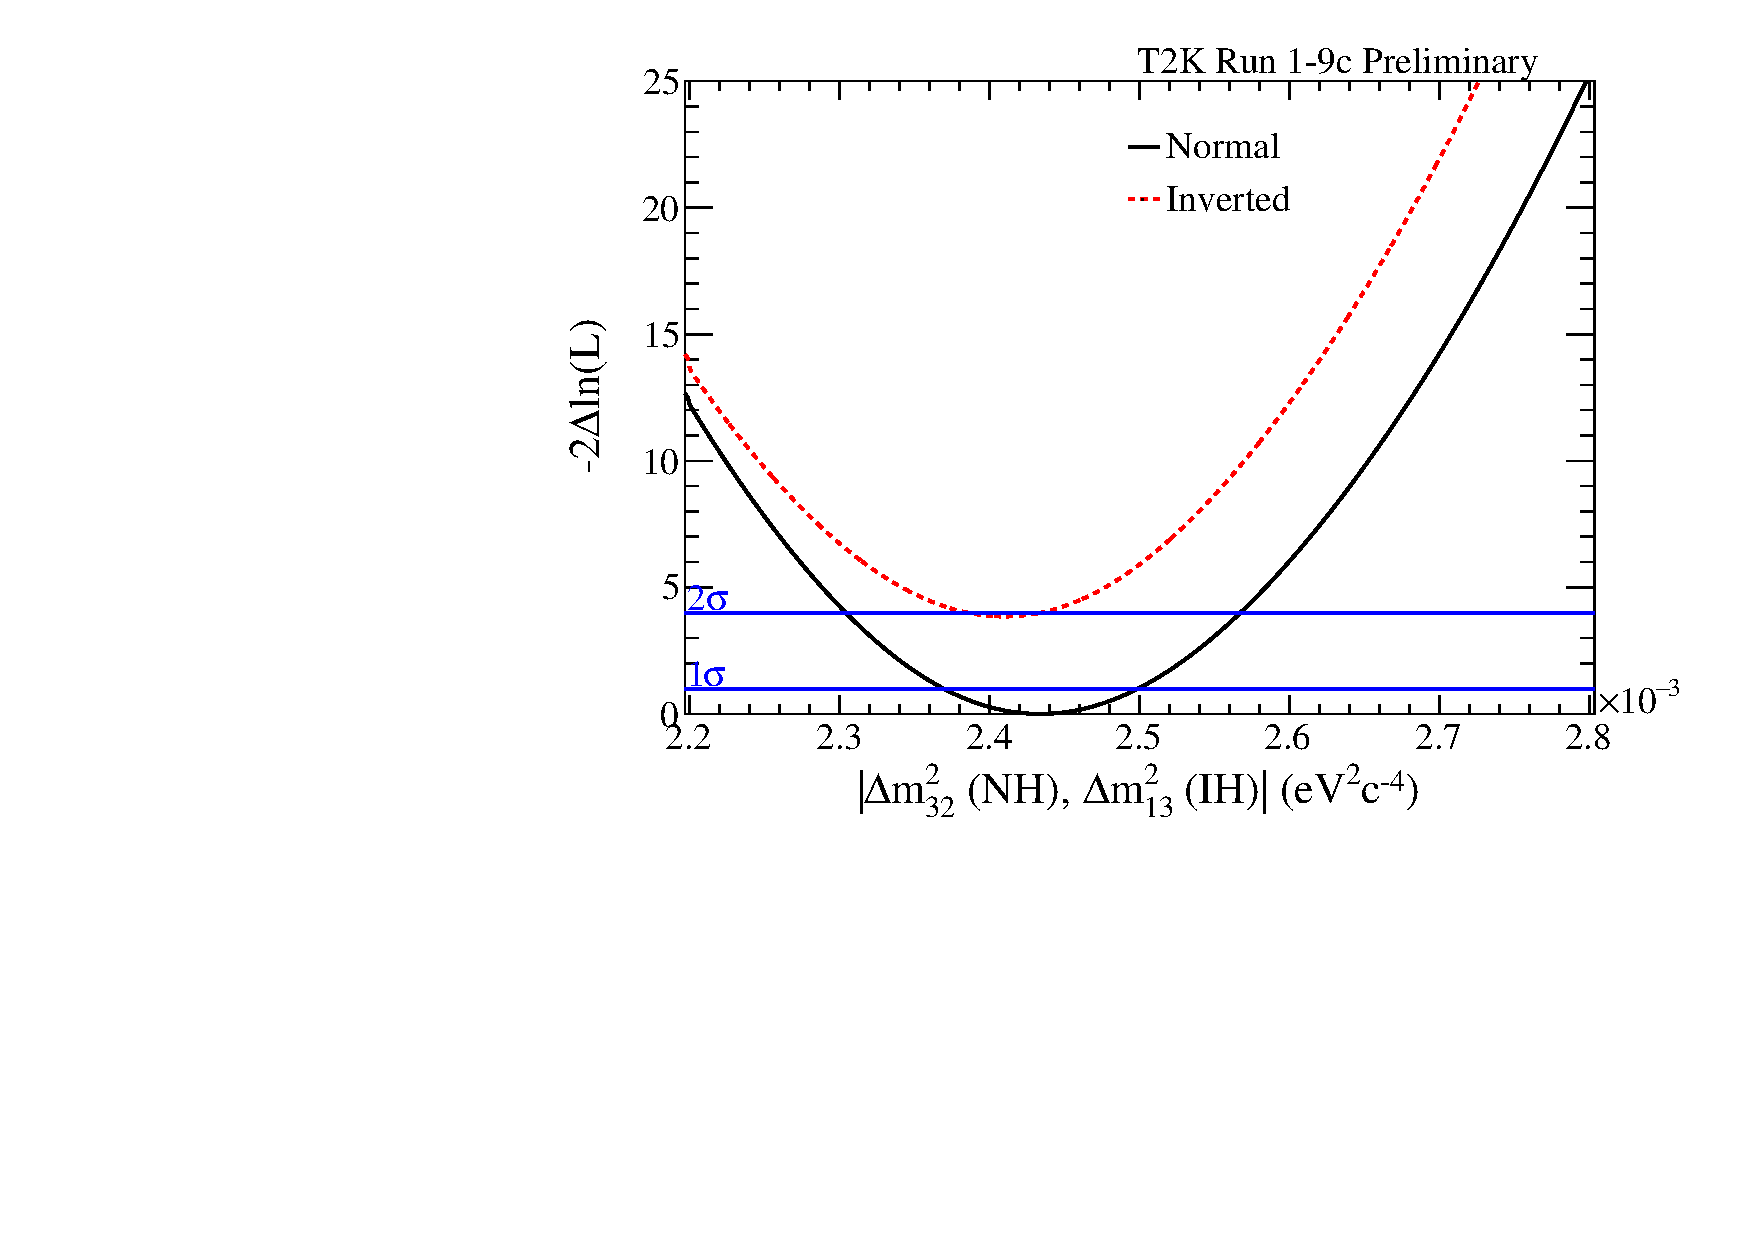
\includegraphics[width=0.9\textwidth]{images/data/dmsq23_data_reactor_global}
		\caption{\dmsq with reactor constraint}
	\end{subfigure}
	\begin{subfigure}[b]{0.49\textwidth}
		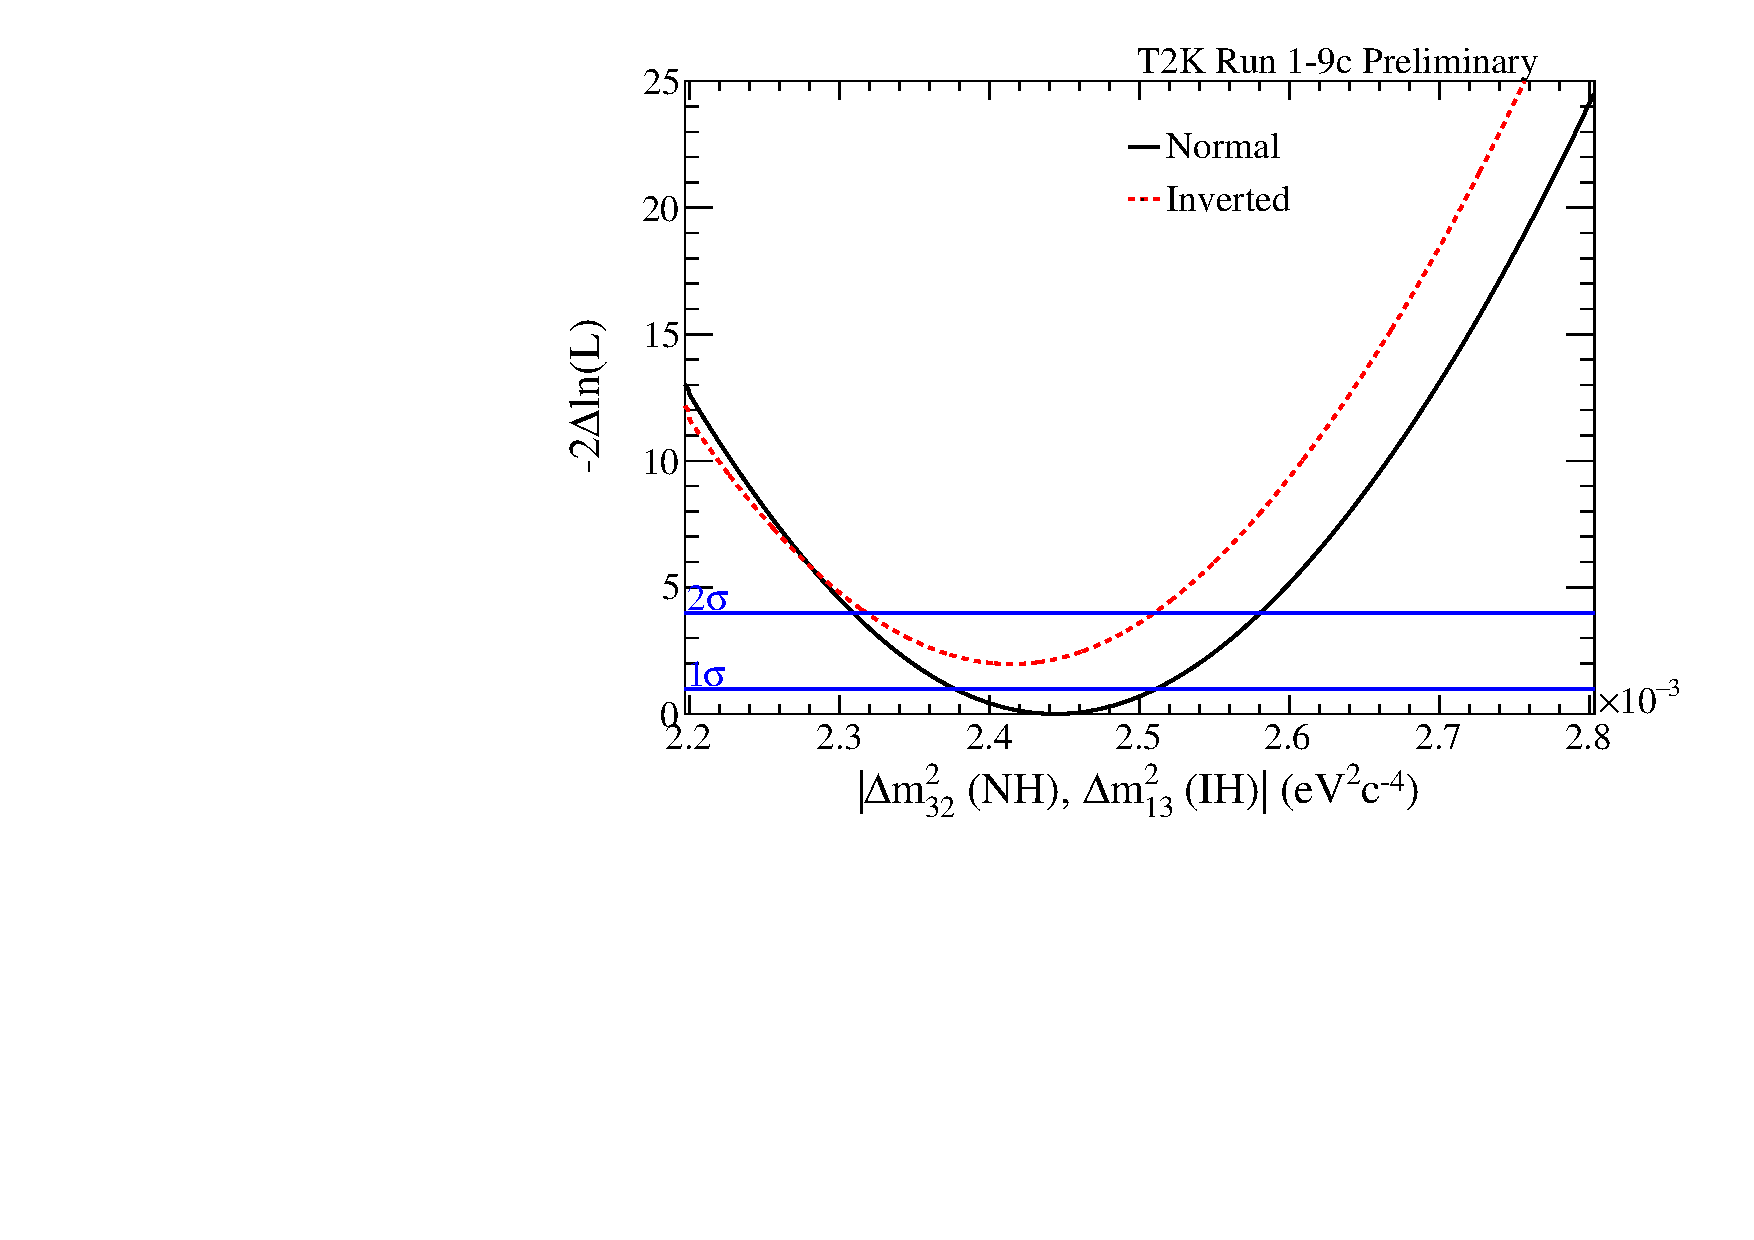
\includegraphics[width=0.9\textwidth]{images/data/dmsq23_data_t2k_global}
		\caption{\dmsq T2K only}
	\end{subfigure}
	\caption {
		The expected $\Delta\chi^2$ distribution as a function of \dmsqtwothree with and without reactor constraint. The mass hierarchy is minimized, with normal and inverted hierarchy $\Delta\chi^2$ distributions shifted to the same global best-fit $\chi^2$ value, which is taken to be the minimum between normal and inverted hierarchy. All 5 samples were used to produce these fits.
	}
	\label{fig:dmsq23_data}
\end{figure*}

\subsection {Feldman-Cousins simultaneous fit of \deltacp and mass hierarchy}
\label{sec:fc_significance}

This section presents the results of the Feldman-Cousins fit of \deltacp and mass hierarchy. The method is the same as that used in \cite{OurRun18JointAnalysis3Flavour}, in particular throws of oscillation parameters are made according to PDG 2016 best-fit values and errors for \ssqthonethree, \ssqthonetwo and \dmsqonetwo, whilst \ssqthtwothree and \dmsq are thrown according to the likelihood distribution produced by an Asimov fit using the best-fit from data for these parameters. \deltacp is fixed at one of 9 evenly specified values on the range $\left[-\pi,\pi\right]$.

\subsubsection{Input oscillation parameters}
\label{sec:fc_significance:inputs}

The distributions of oscillation parameters are shown in \cref{fig:fc_input_dist}.

\begin{figure*}[htb]
	\center
	\begin{subfigure}[b]{0.49\textwidth}
		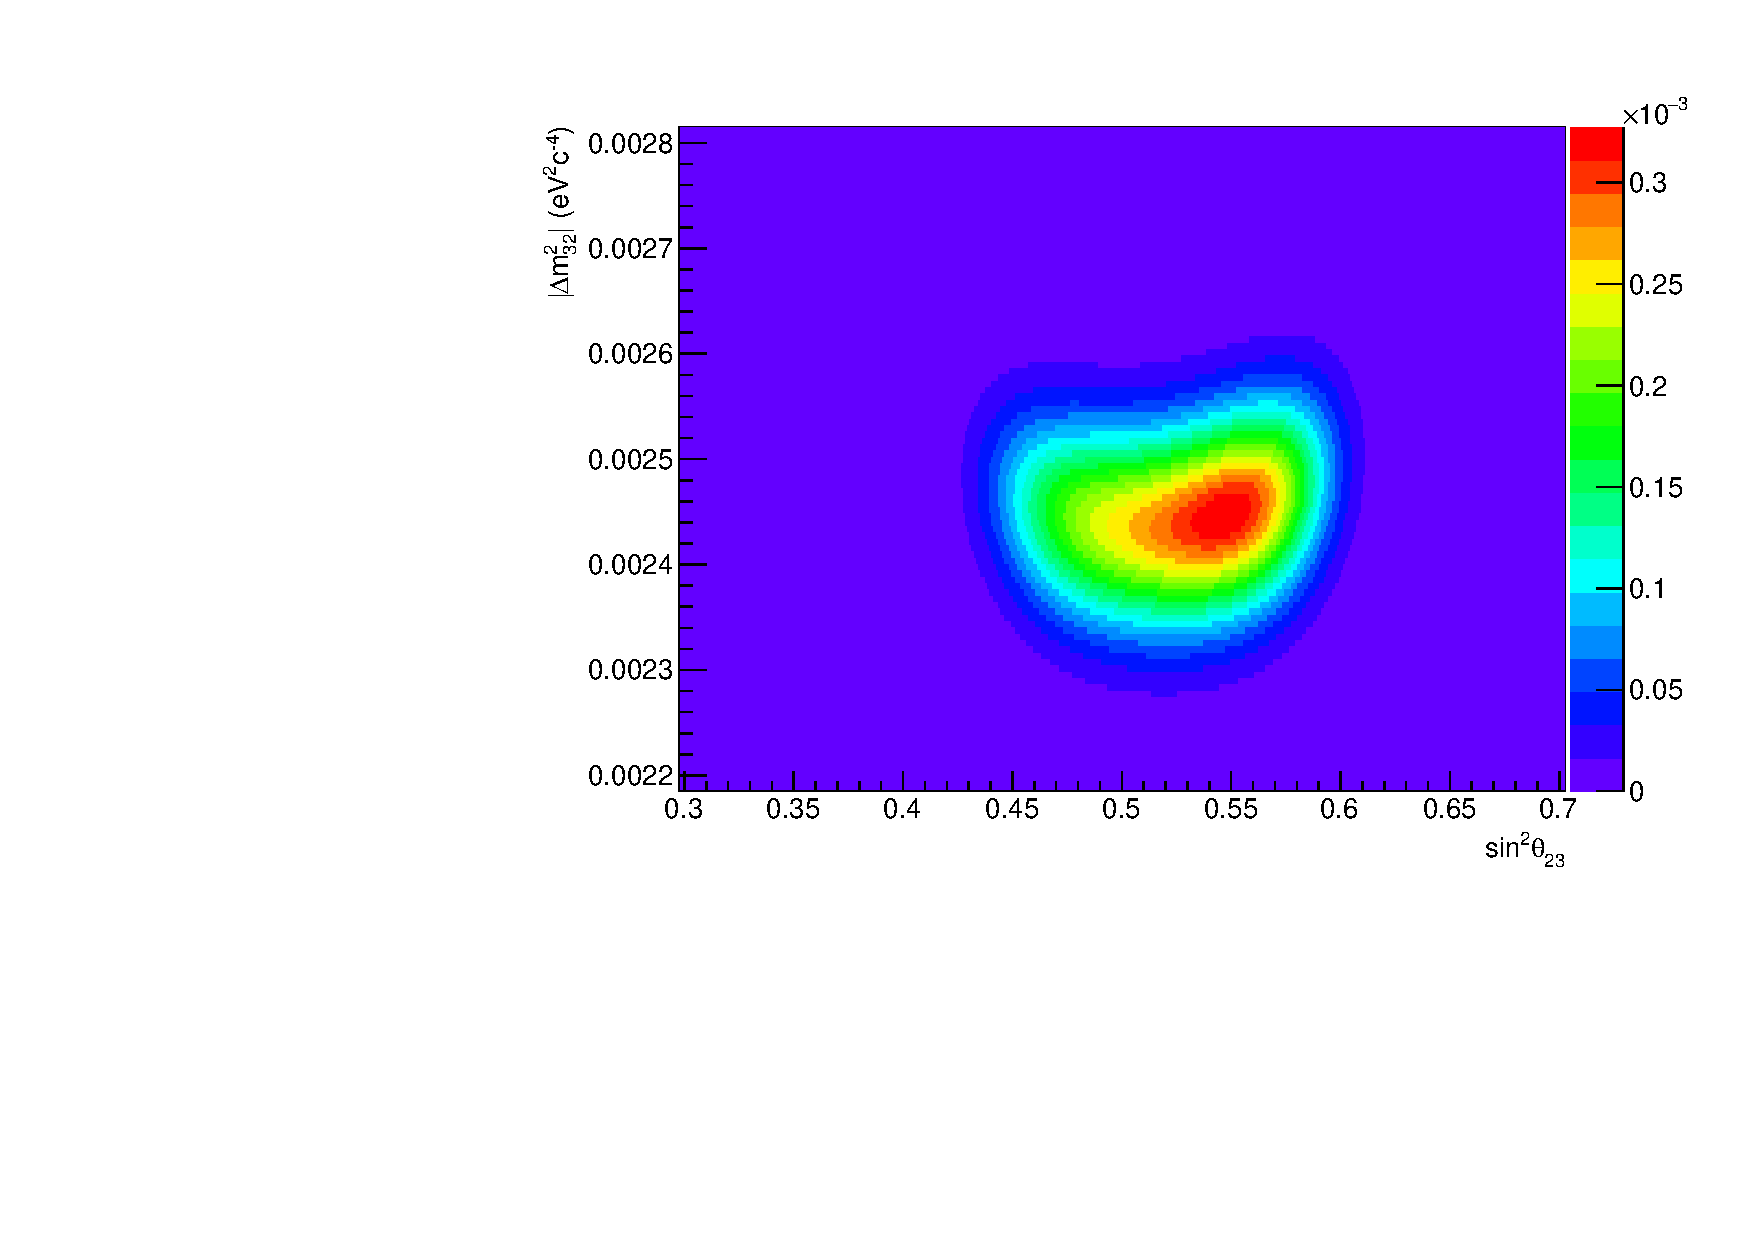
\includegraphics[width=0.9\textwidth]{images/fc/inputs/disappearance_nh_likelihood}
		\caption{Normal hierarchy}
	\end{subfigure}
	\begin{subfigure}[b]{0.49\textwidth}
		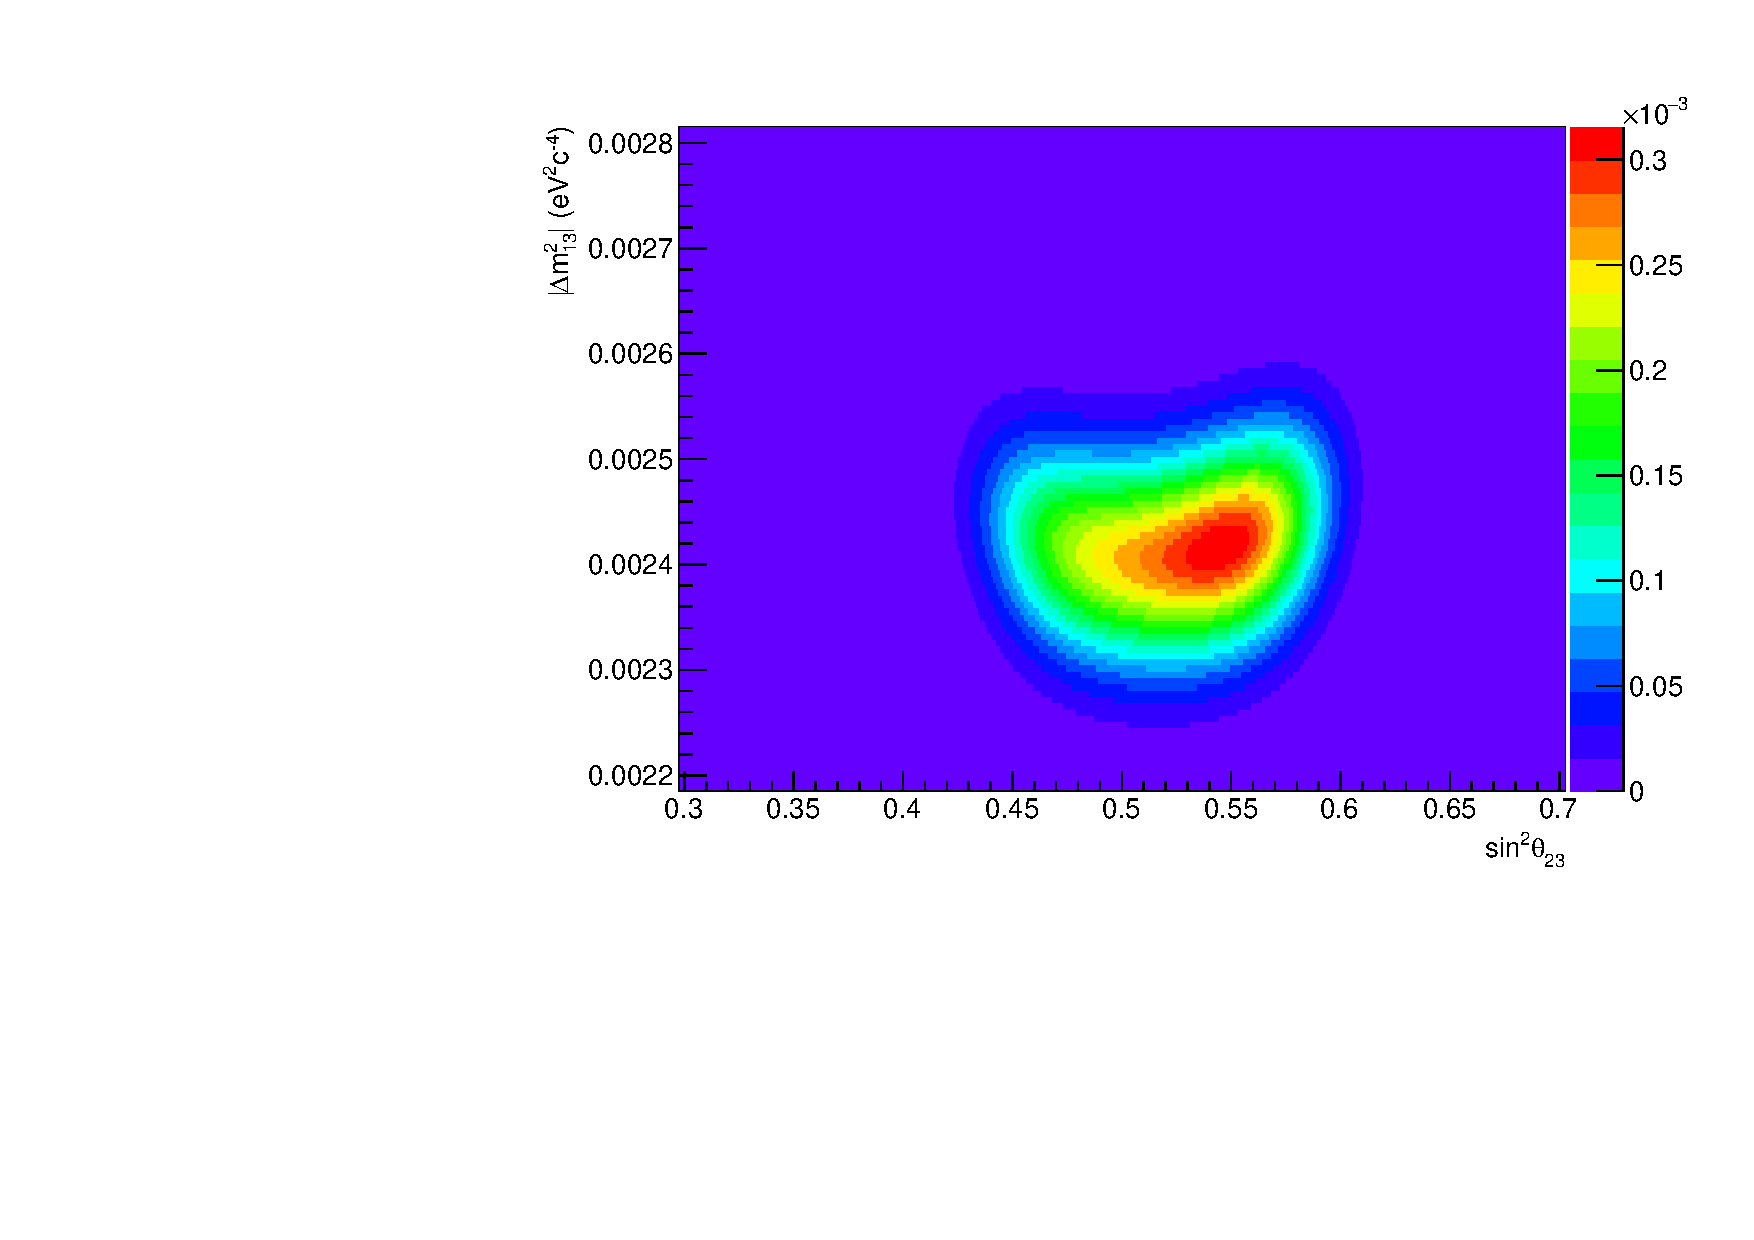
\includegraphics[width=0.9\textwidth]{images/fc/inputs/disappearance_ih_likelihood}
		\caption{Inverted hierarchy}
	\end{subfigure}
	\begin{subfigure}[b]{0.49\textwidth}
		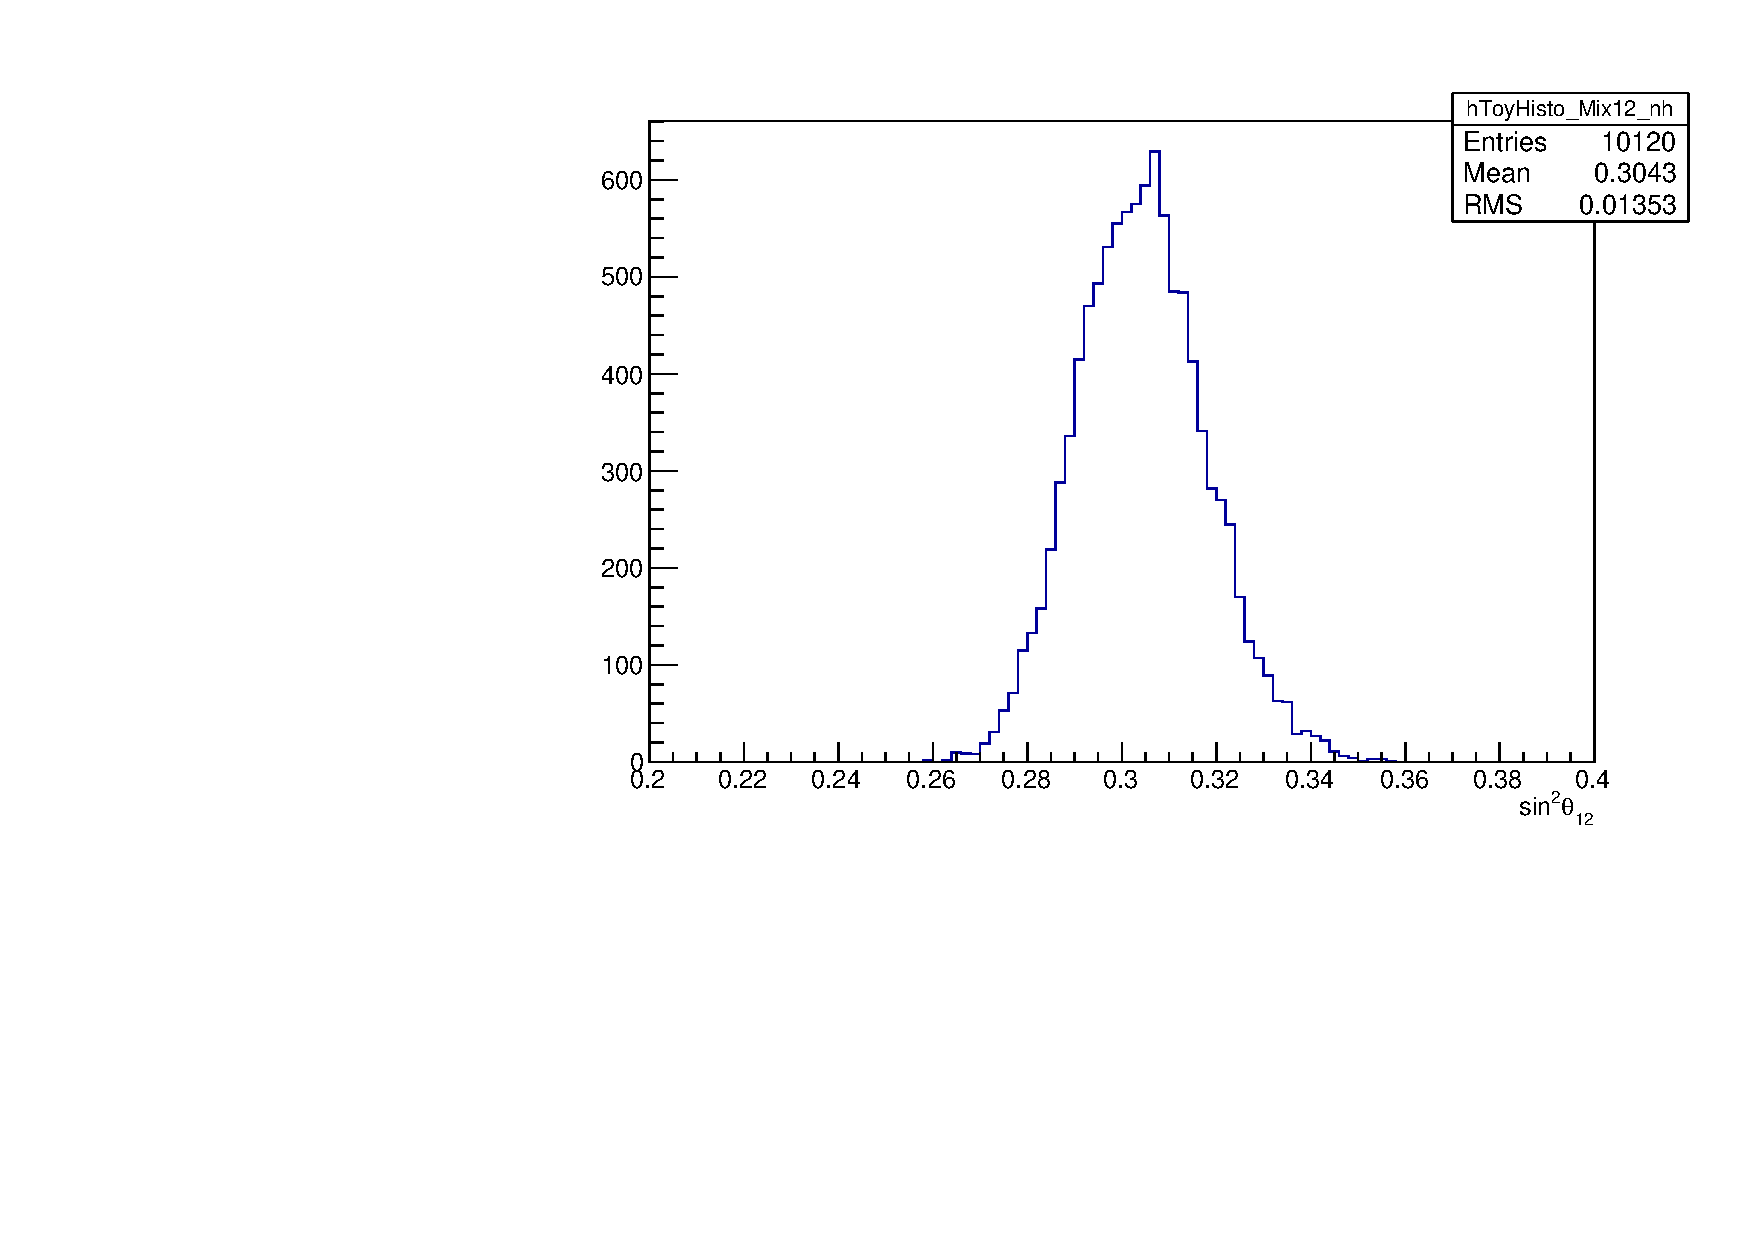
\includegraphics[width=0.9\textwidth]{images/fc/inputs/mixing12_in}
		\caption{\ssqthonetwo}
	\end{subfigure}
	\begin{subfigure}[b]{0.49\textwidth}
		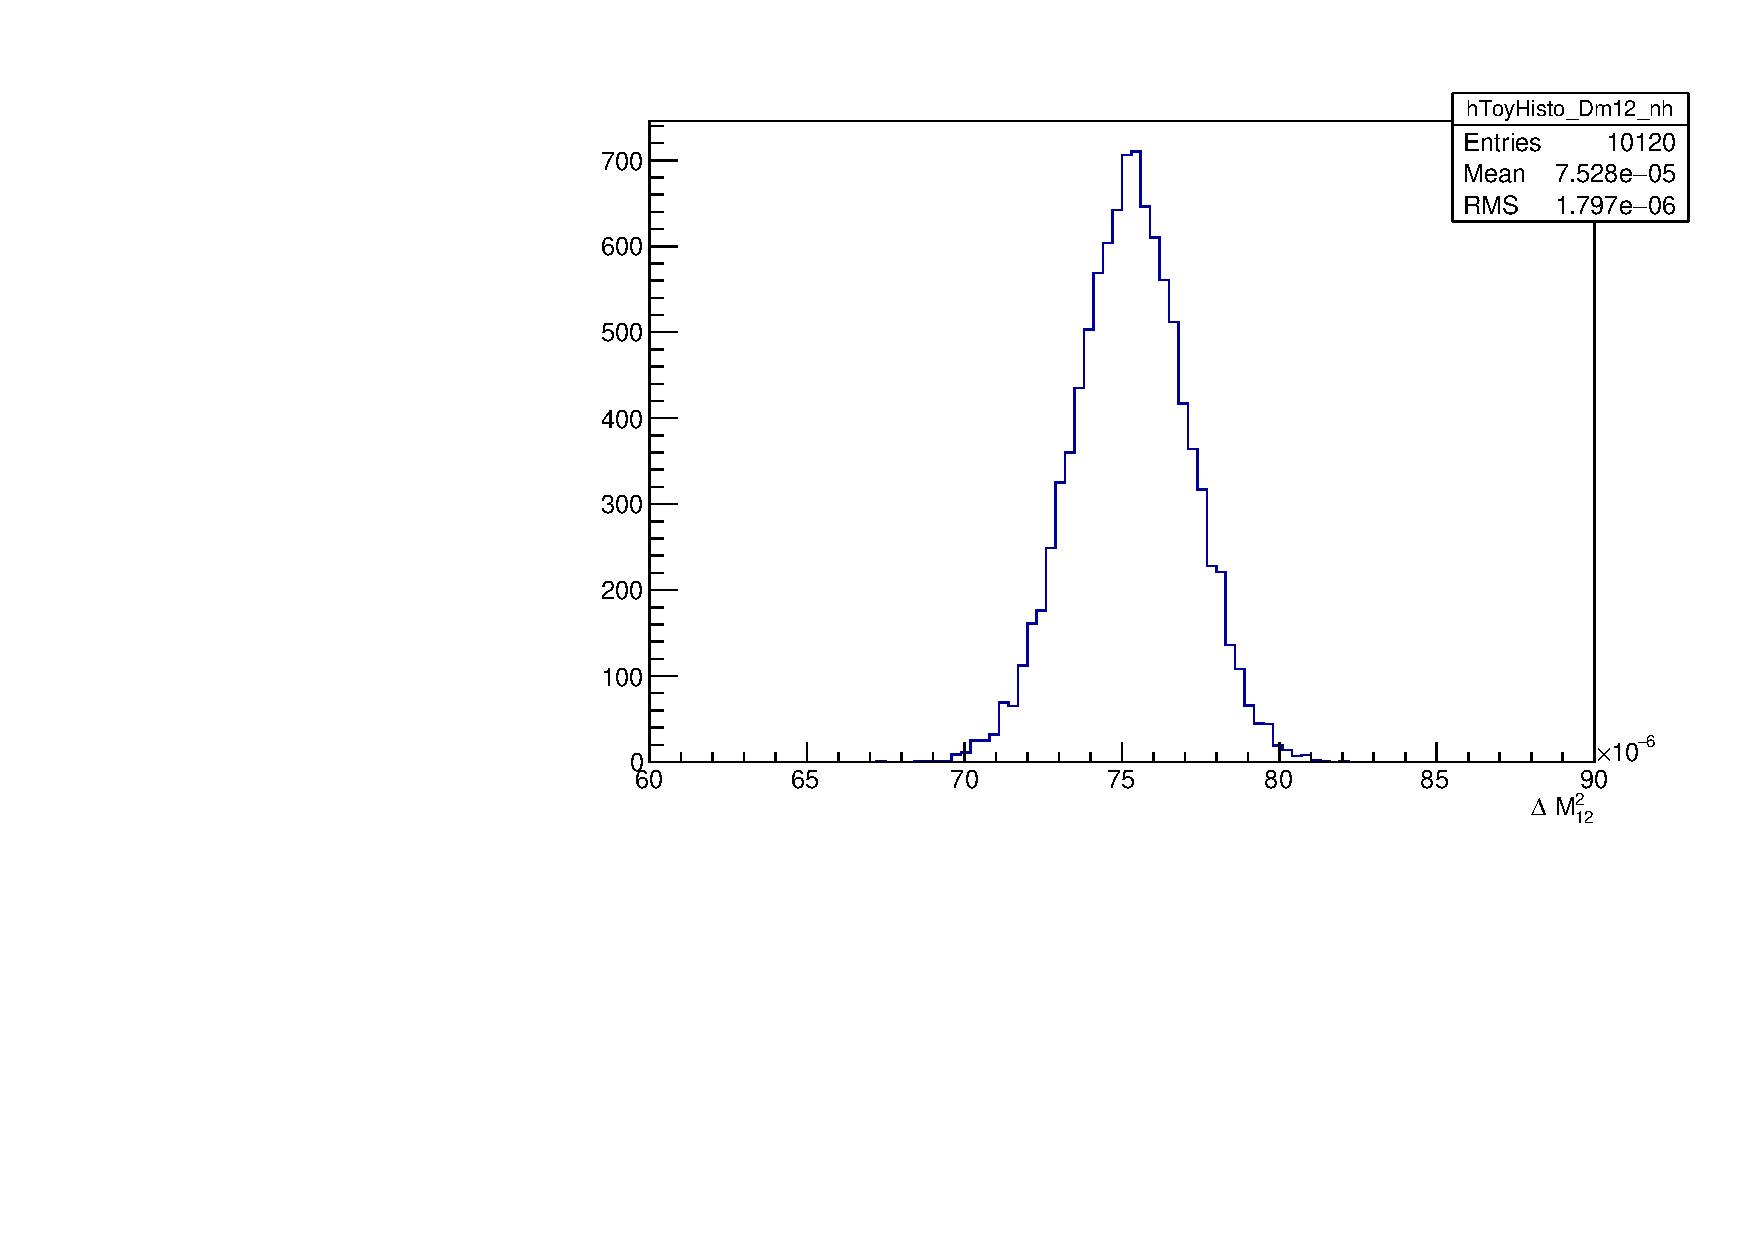
\includegraphics[width=0.9\textwidth]{images/fc/inputs/dm12_in}
		\caption{\dmsqonetwo}
	\end{subfigure}
	\begin{subfigure}[b]{0.49\textwidth}
		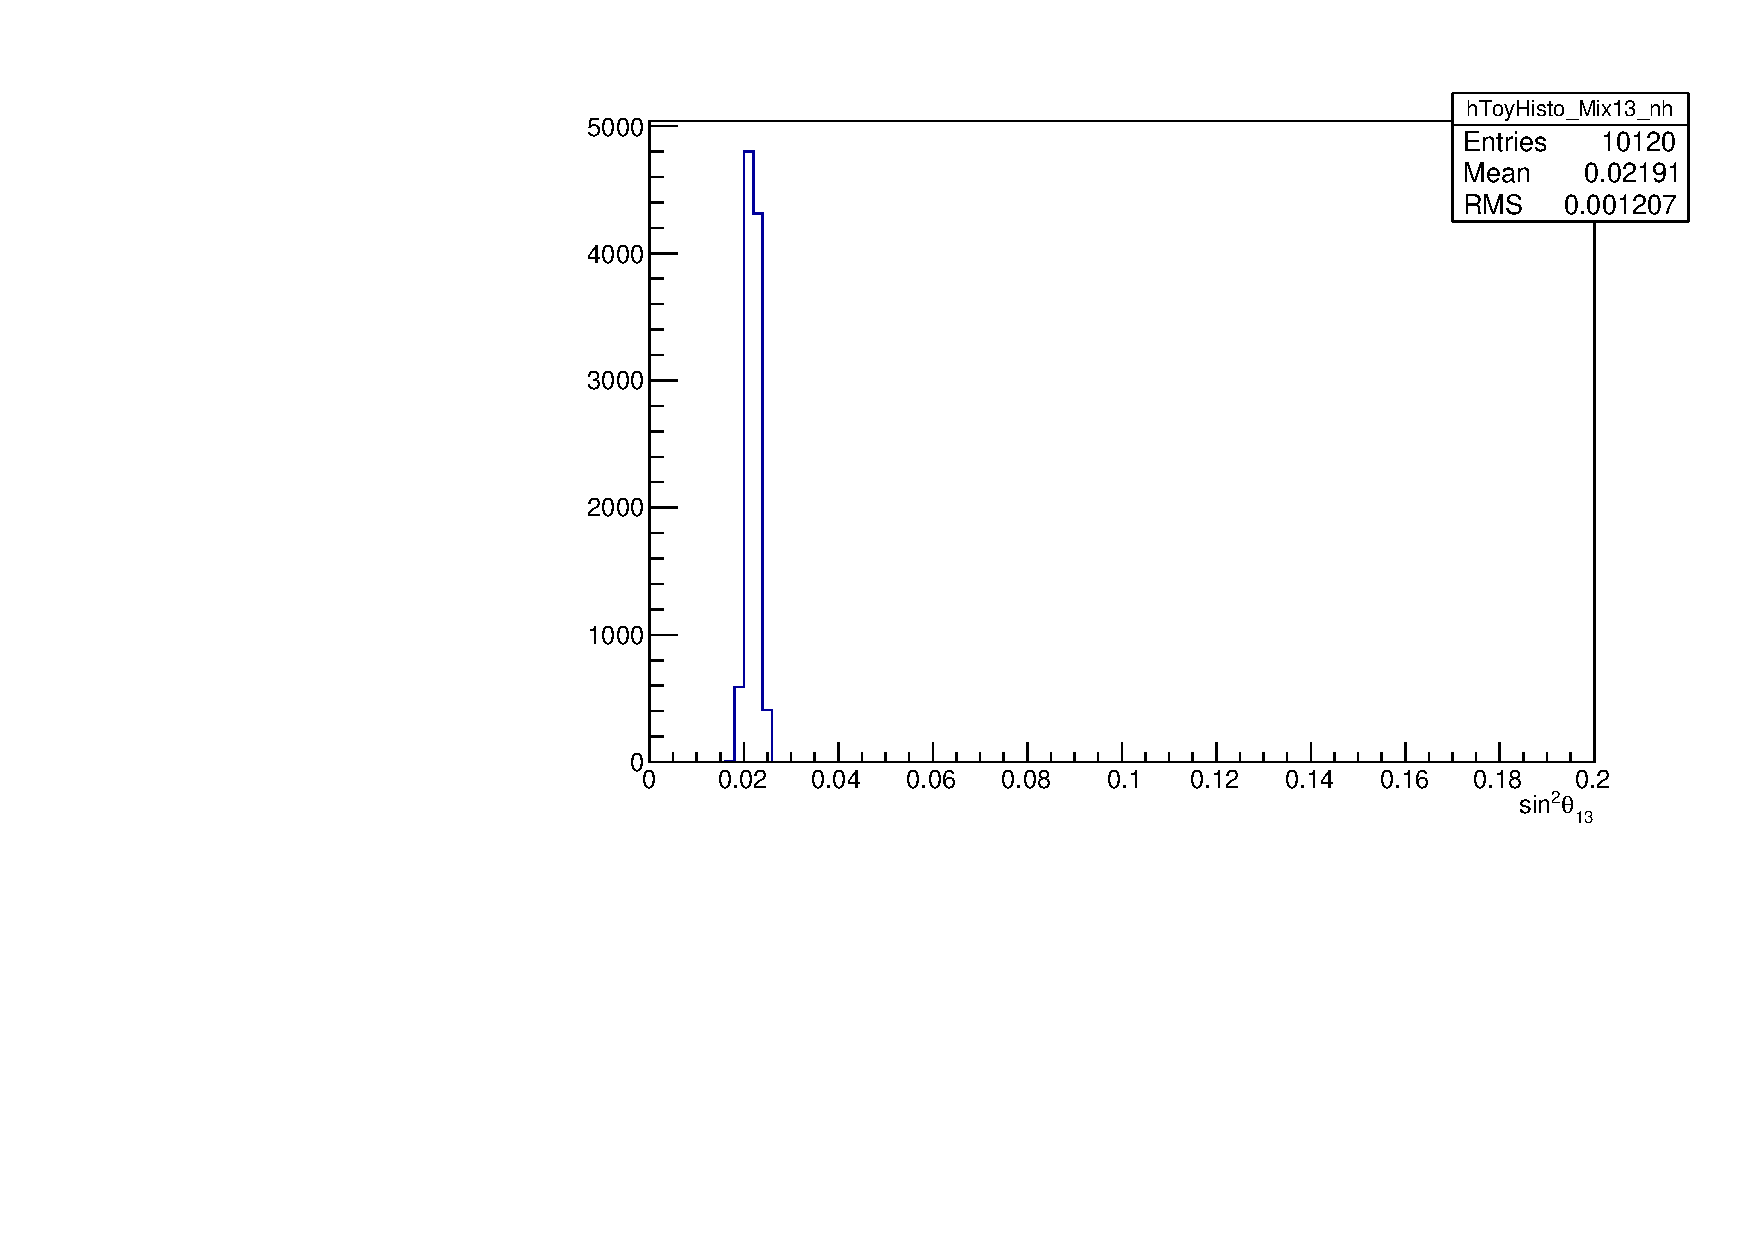
\includegraphics[width=0.9\textwidth]{images/fc/inputs/mixing13_in}
		\caption{\ssqthonethree}
	\end{subfigure}
	\caption {
		Distribution of oscillation parameter throws for Feldman-Cousins fits.
	}
	\label{fig:fc_input_dist}
\end{figure*}

\subsubsection{Feldman-Cousins critical values and confidence intervals}
\label{sec:fc_significance:intervals}
In \cref{fig:fc_interval} the confidence intervals obtained with the Feldman-Cousins method are shown for \deltacp and mass hierarchy with reactor constraint for the \RunPeriod data set. The critical values at \color{blue}$1\sigma$, 90\% and $2\sigma$ CL\color{black} are computed for both the mass hierarchies at the following true values of \deltacp; $-\pi$, $-3\pi/4$, $-\pi/2$, $-\pi/4$, 0, $+\pi/4$, $+\pi/2$, $+3\pi/4$, and $+\pi$. Inverted hierarchy is almost excluded at $2\sigma$, except for a small interval around $\delta_{CP} = -\pi/2$. Both $\delta_{CP} = 0$ and $\delta_{CP} = \pi$ are excluded at $2\sigma$. In \cref{tab:fc_interval} the $2\sigma$ CL intervals for \deltacp versus mass hierarchy, obtained with the Feldman-Cousins method, are shown. Comparison of critical values between VALOR and p-theta are provided in \cref{app:fc_compare}.

\begin{figure*}[htb]
	\center
	\begin{subfigure}[b]{0.6\textwidth}
		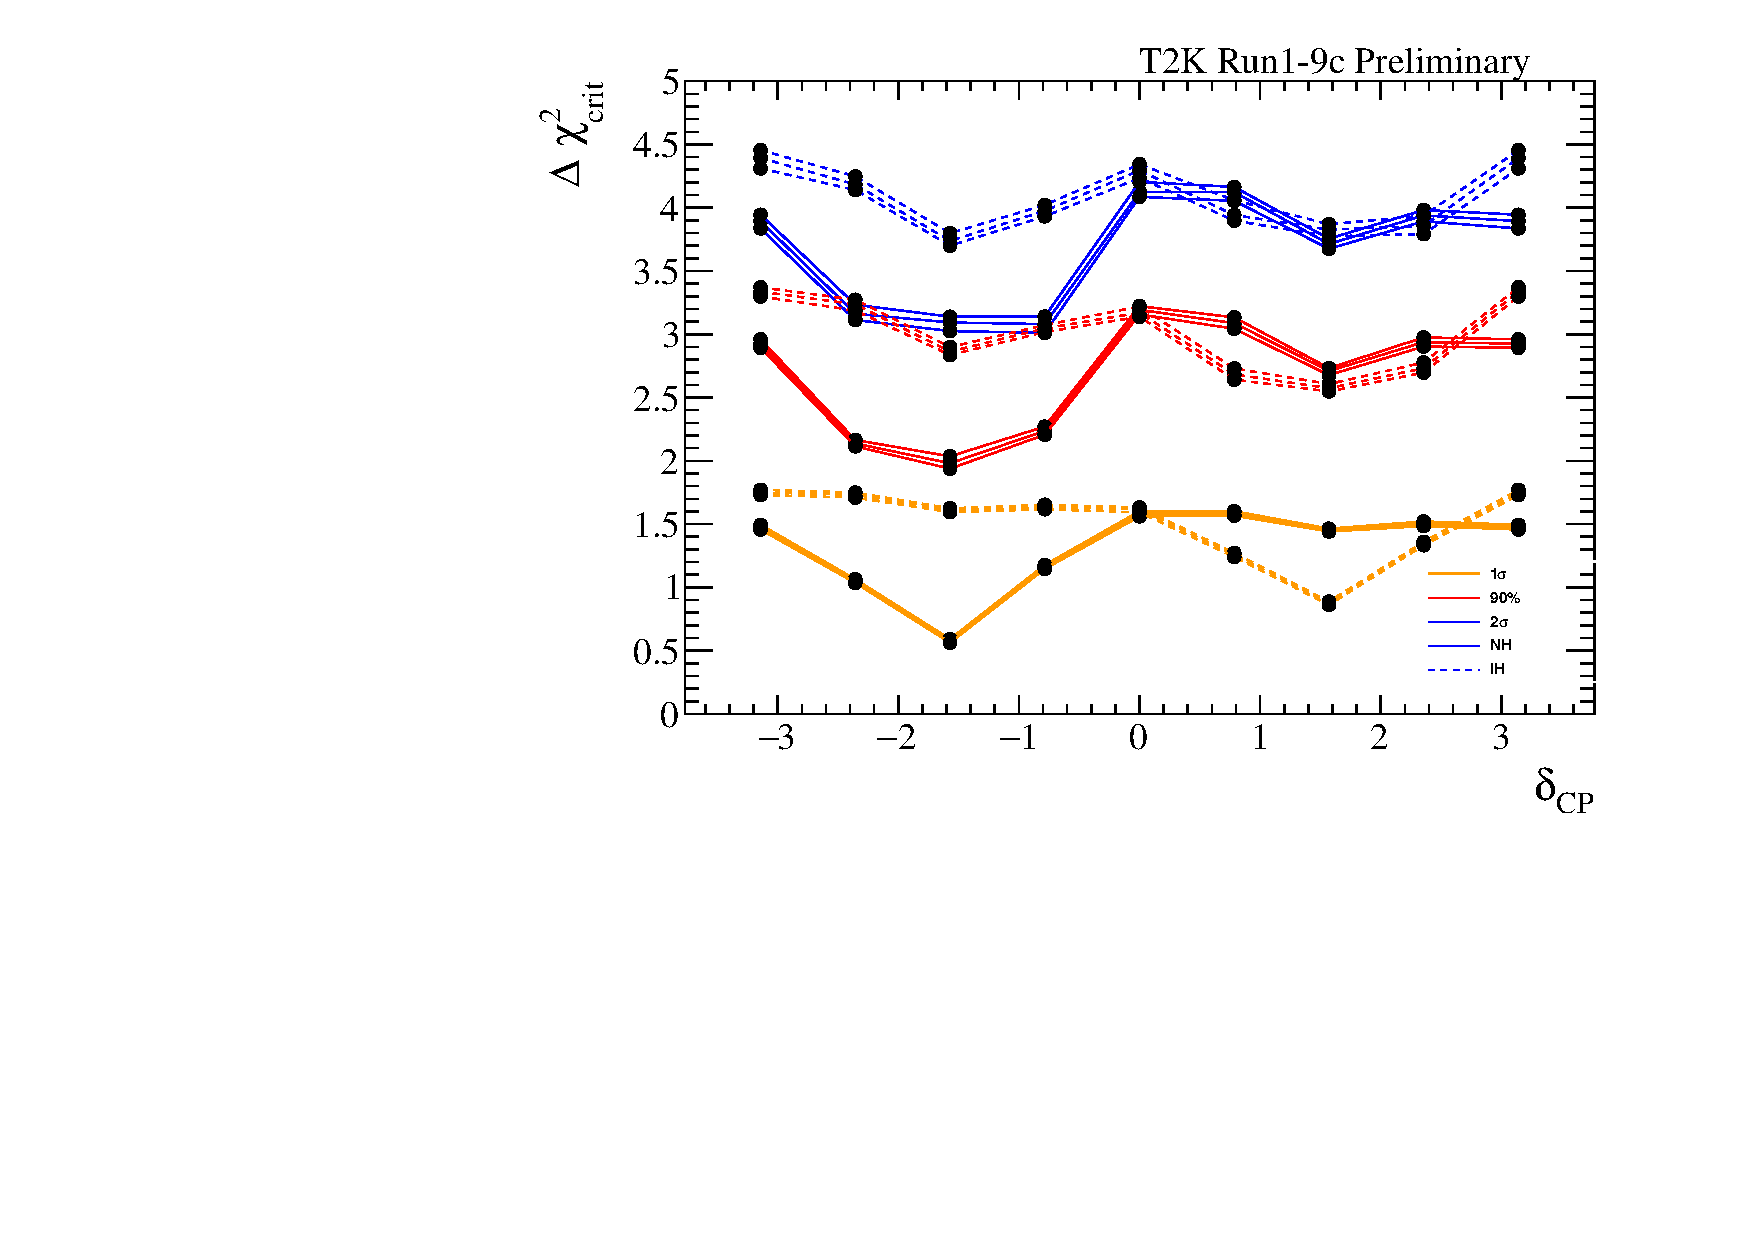
\includegraphics[width=0.9\textwidth]{images/fc/FC_critical_values}
		\caption{\label{fig:fc_critval}Critical $\Delta\chi^2$ values}
	\end{subfigure}
	\begin{subfigure}[b]{0.49\textwidth}
		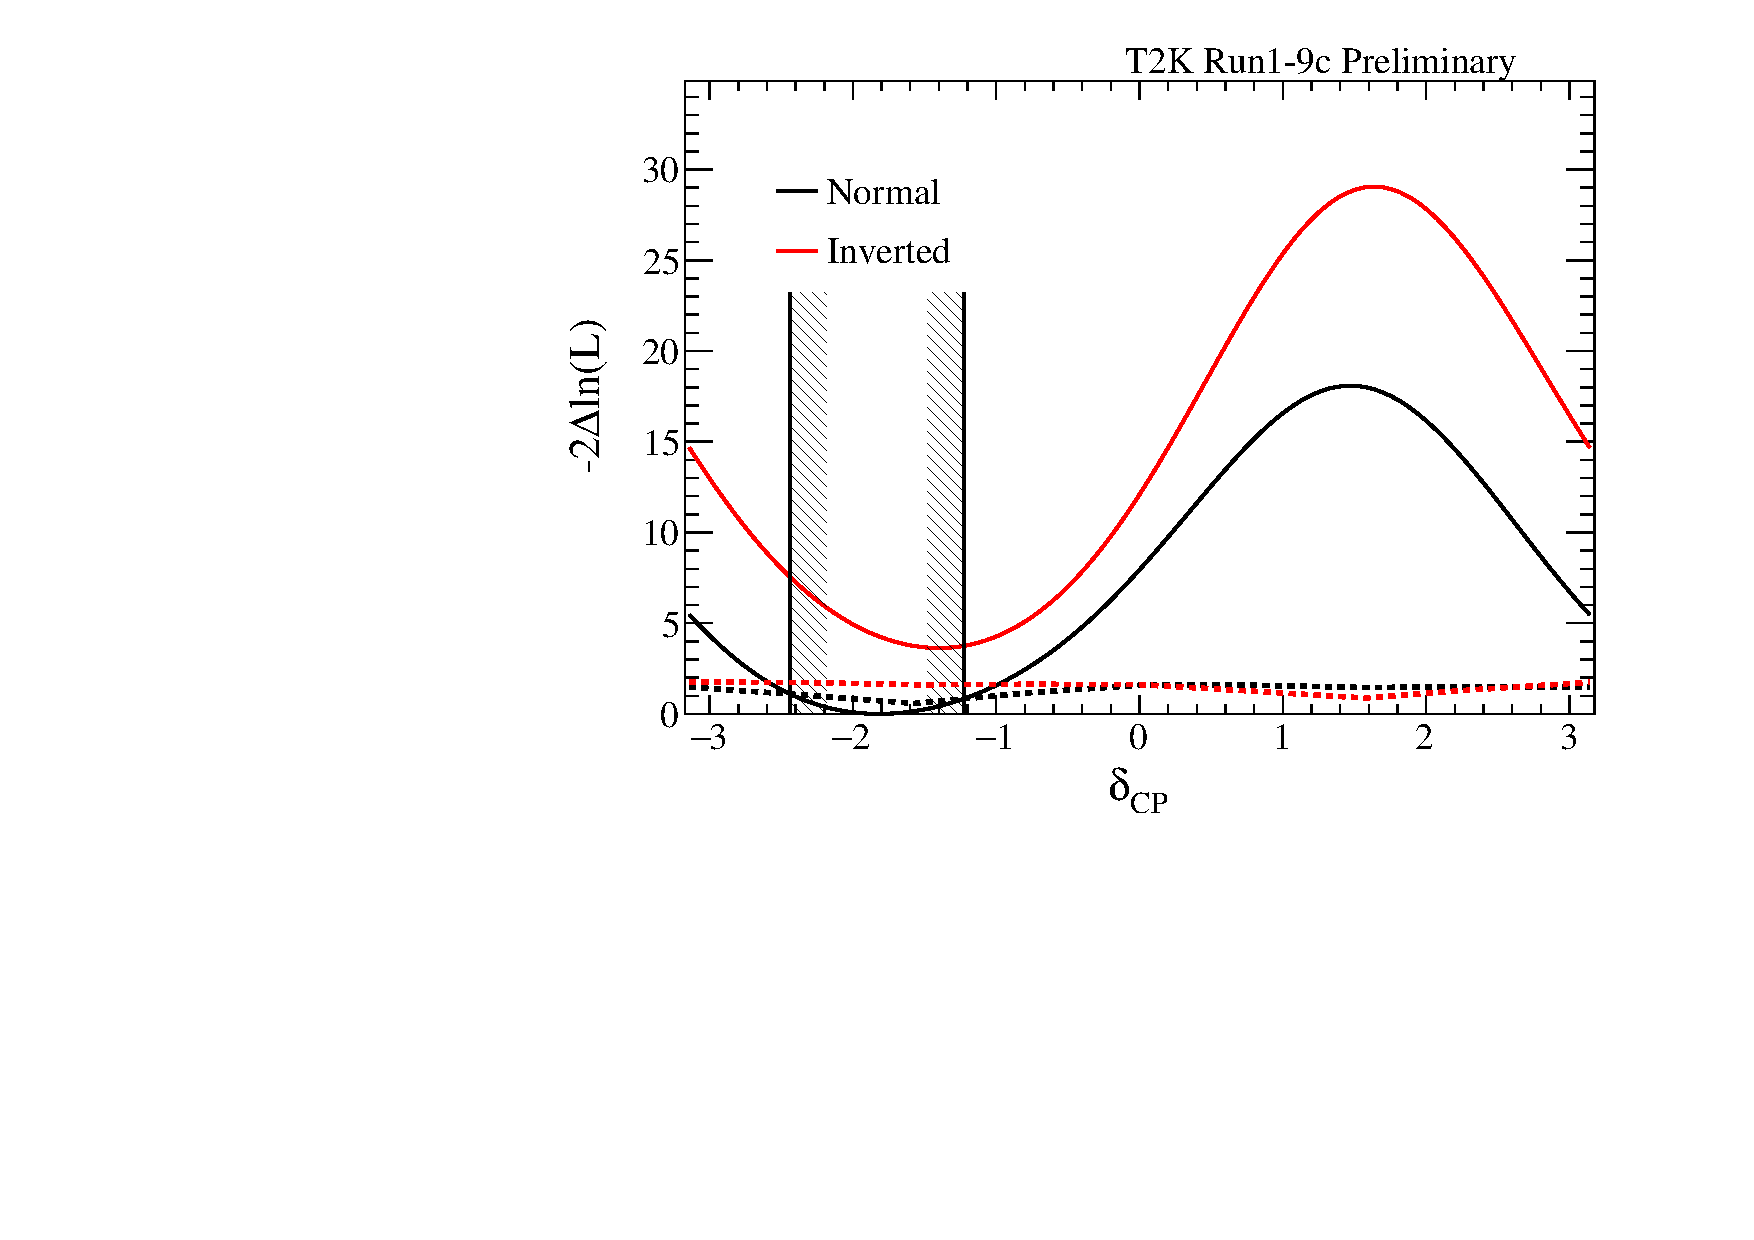
\includegraphics[width=0.9\textwidth]{images/fc/deltacp_mpi2_1sigma_critval}
		\caption{$1\sigma$ CL exclusion region}
	\end{subfigure}
	\begin{subfigure}[b]{0.49\textwidth}
		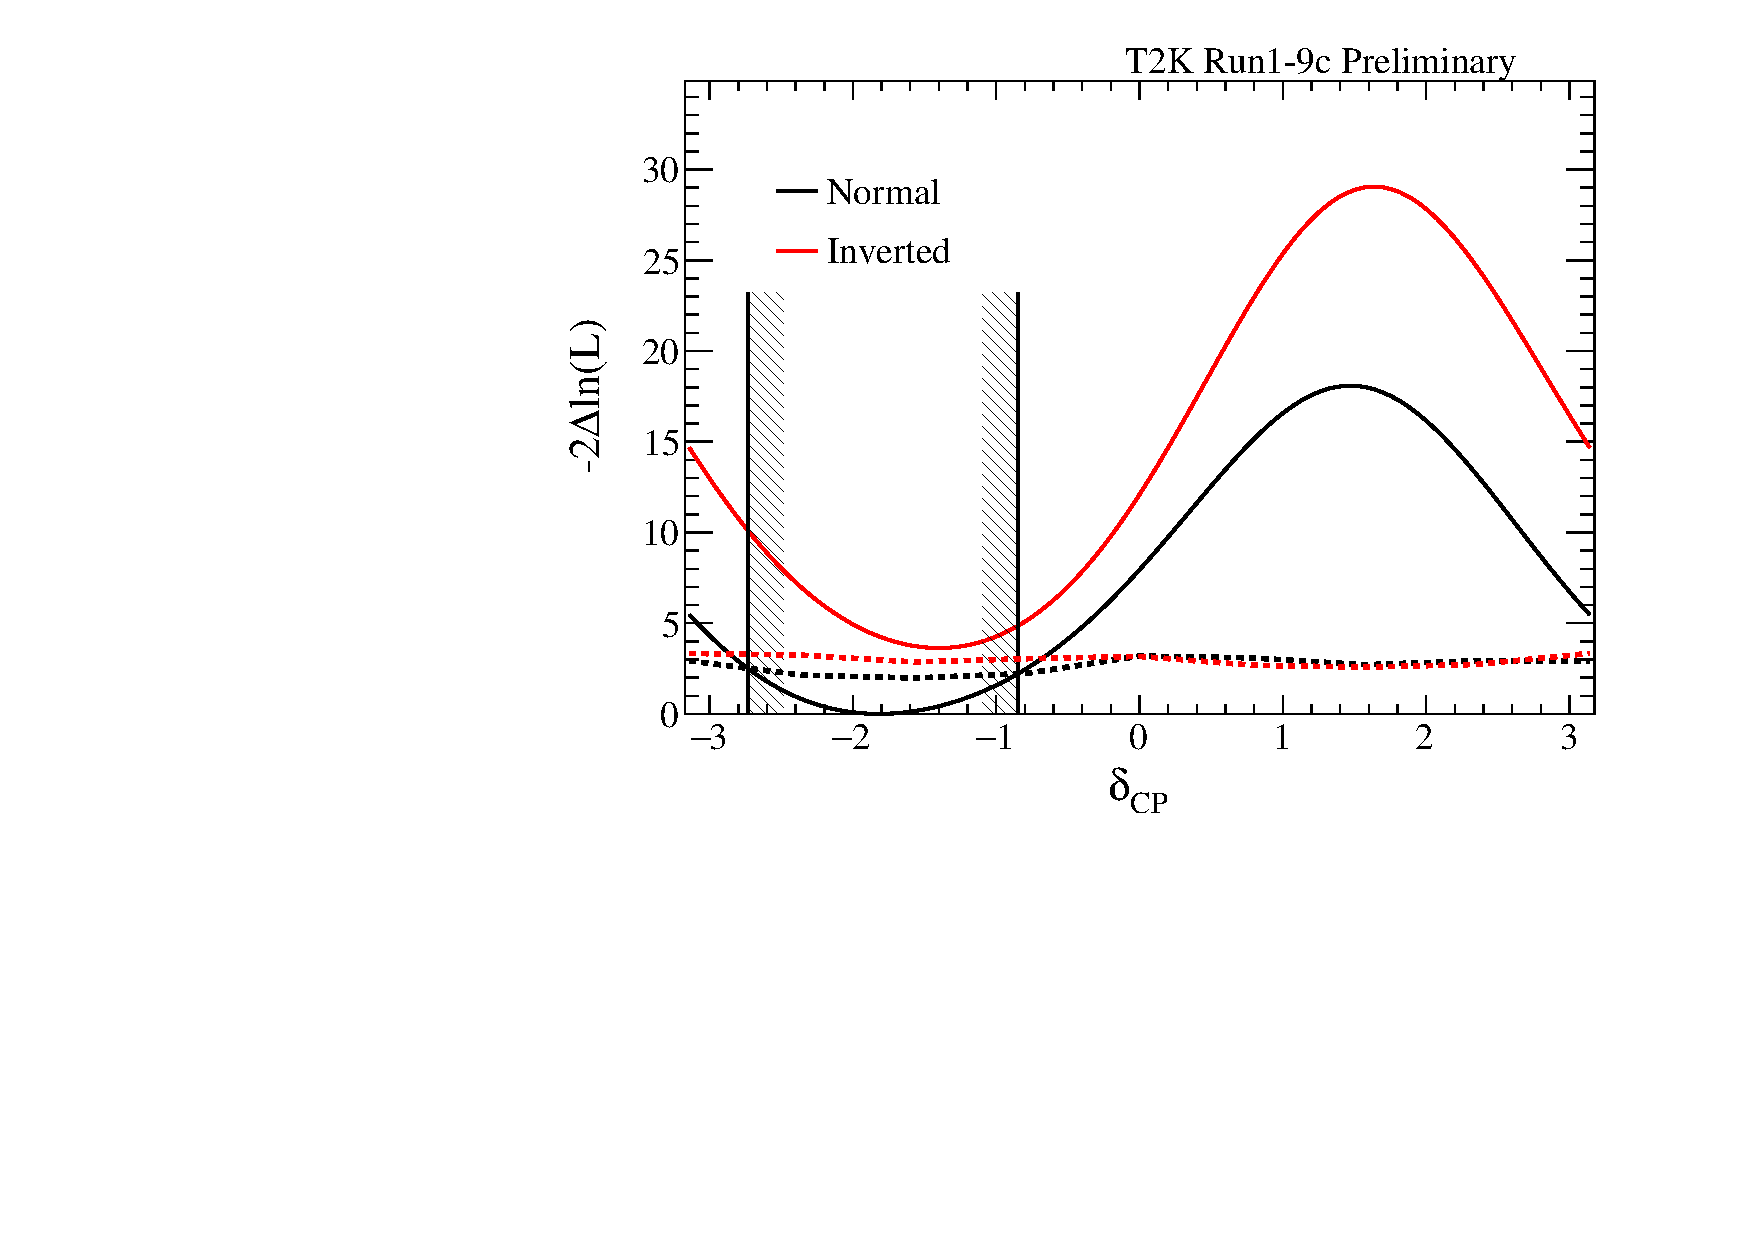
\includegraphics[width=0.9\textwidth]{images/fc/deltacp_mpi2_90CL_critval}
		\caption{90\% CL exclusion region}
	\end{subfigure}
	\begin{subfigure}[b]{0.49\textwidth}
		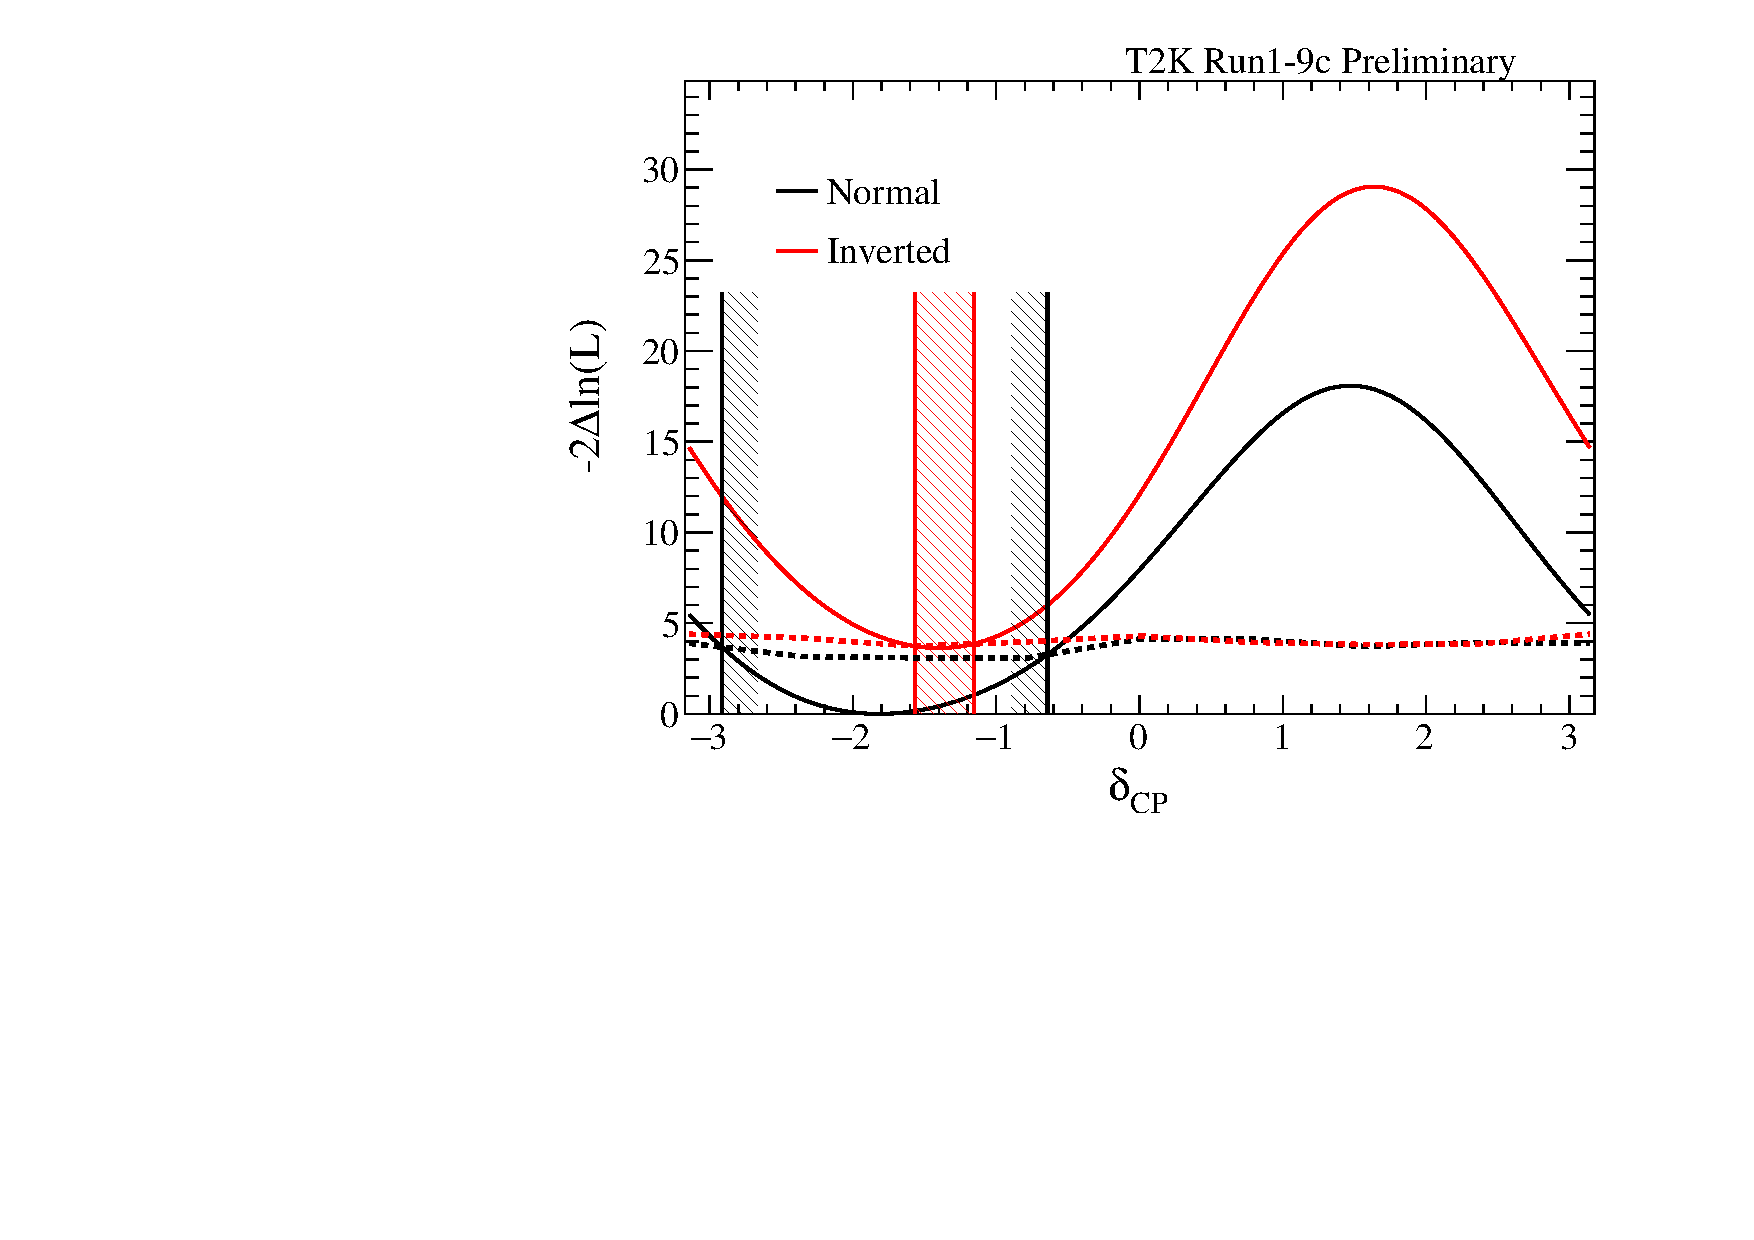
\includegraphics[width=0.9\textwidth]{images/fc/deltacp_mpi2_2sigma_critval}
		\caption{$2\sigma$ CL exclusion region}
	\end{subfigure}
	\caption {
$\Delta\chi^2$ critical values and confidence intervals for the measured $\Delta\chi^2$ distributions for \RunPeriod. Critical values obtained with the Feldman-Cousins method for \RunPeriod for 9 evenly spaced values on the range \( \left[-\pi,\pi\right] \). Critical values are shown for 1\( \sigma \), 2\( \sigma \) and 90\% CL for normal (solid lines) and inverted (dashed lines) hierarchies. At least \num{1e4} toy experiments are performed for each point. The three bands of lines show the \( \pm 1\sigma \) uncertainty on the critical values. Also shown are the measured \( \Delta \chi^2 \) distributions shifted with respect to the same global minium and the $1\sigma$, 90\% and $2\sigma$ exclusion regions for both mass hierarchies. 
	}
	\label{fig:fc_interval}
\end{figure*}

\begin{table}[htb]
	\centering
	\begin{tabular}{| c | c | c | c | c |}
\hline
Parameter & Reactor & CL & Normal hierarchy & Inverted hierarchy \\
\hline
\deltacp		& Yes & $ 1\sigma $ & $\left[ -2.437, -1.228 \right]$ & - \\
\deltacp		& Yes & 90\% & $\left[ -2.735, -0.849 \right]$ & - \\
\deltacp		& Yes & $ 2\sigma $ & $\left[ -2.914, -0.642 \right]$ & $\left[ -1.569, -1.158 \right]$ \\
\hline
\end{tabular}

	\caption{
		The confidence intervals at $1\sigma$, 90\% and $2\sigma$ CL obtained with the Feldman-Cousins method for the \RunPeriod data set is shown for the measurement of \deltacp versus mass hierarchy.
	}
	\label{tab:fc_interval}
\end{table}
\FloatBarrier
\subsection {Discussion of the \RunPeriod data fit results}
\label{sec:results:discussion}

With FHC POT little changed from the previous analysis, the level of agreement between data and Asimov A expectation is little changed; in particular, we continue to see an excess in the number of observed appearance events in the \nueCConepi data set (\NskObservedNueCConepi{})  compared to the Asimov A expectation (\NAsimovAExpectationNueCConepi{}), one ring $e$-like sample continues to show good agreement between observed (\NskObservedNue{}) and expected (\NAsimovAExpectationNue{}) events and we continue to see a deficit in observed (\NskObservedNumu{}) \color{blue}relative to \color{black} expected (\NAsimovAExpectationNumu) events in the one ring $\mu$-like sample.

In RHC, where POT is increased by $\sim49$\%, we continue to see good agreement between observed (\NskObservedNueBar{}) and expected (\NAsimovAExpectationNueBar{}) events in the one-ring $e$-like sample, and between observed (\NskObservedNumuBar{}) and expected (\NAsimovAExpectationNumuBar) events in the one-ring $\mu$-like sample.

The value of \deltacp favoured by the joint fit analysis, when the reactor constraint is applied, is \BestFitDeltacpwRC (corresponding to normal hierarchy), close to $\delta_{CP} = -\pi / 2$ and rejects CP-conservation at the $2\sigma$ level when using the reactor constraint, both for the constant $\Delta\chi^2$ and the Feldman-Cousins methods. The new analysis excludes a slightly larger range of values of $\delta_{CP}$ in both hierarchies, relative to the previous analysis. If the reactor constraint is not applied, the best-fit value of \deltacp is \BestFitDeltacpwoRC (normal hierarchy).

The appearance fit excludes CP-conservation at the 90\% level in normal hierarchy, whilst the value of \ssqthonethree in this 2D fit is in agreement with the PDG 2016 value at the $1\sigma$ level. 

In the 1D fit, T2K favours a normal hierarchy best-fit value for \ssqthonethree of \BestFitMixingOneThreewoRC. The 1D contour is in agreement with the PDG 2016 value ($0.0219 \pm 0.0012$) at $\sim1.1\sigma$ (see \cref{tab:data_bestfit}).

The value of \ssqthtwothree favoured by the analysis is \BestFitMixingTwoThreewRC (\BestFitMixingTwoThreewoRC) with (without) the reactor constraint and corresponds to normal hierarchy, with the 1D contours in agreement with and without the reactor constraint at $1 \sigma$, furthermore, the constraint is consistent with maximal mixing at the $1\sigma$ level, as seen in our previous analyses.

The value of \dmsqtwothree favoured by the analysis is \BestFitDmTwoThreewRC $\times 10^{-3}\text{ eV}^2\text{/c}^4$ (\BestFitDmTwoThreewoRC$\times 10^{-3}\text{ eV}^2\text{/c}^4$) with (without) the reactor constraint and corresponds to normal hierarchy, with the 1D contours in agreement with and without the reactor constraint at $1 \sigma$.

As with the previous analysis, we continue to see stronger constraints in data than expected from Asimov A sensitivity studies for \deltacp and \ssqthtwothree (see \cref{app:data_asimov_comparison}).

\iffalse
When considering the constant $\Delta\chi^2$ method, we see that the constraint on \deltacp is stronger than expected. To investigate the source of this difference a number of fits were undertaken using hybrids of data and MC. In particular \cref{fig:deltacp_hybrids} shows the expected sensitivity from the Asimov A data set (dashed), the data fit (solid black) and then a number of additional fits where one of the data samples was replaced by the corresponding Asimov A sample (e.g. Data x1Rmu indicates a fit of 4 data samples, with the one-ring $\mu$-like sample being replaced by the Asimov A prediction). From this one can see that the largest contribution to the stronger constraint comes from the upward fluctuation observed in the \nueCConepi{} sample, but contributions are also evident from the FHC one-ring $\mu$-like sample, where a deficit in events is seen, and from the two one-ring $e$-like samples. This results in the exclusion of CP-conservation at more than $2 \sigma$ with the reactor constraint applied and the inverted hierarchy is disfavoured at 90\%CL. The effect is also apparent in the appearance contour.

\begin{figure*}[htb]
	\center
	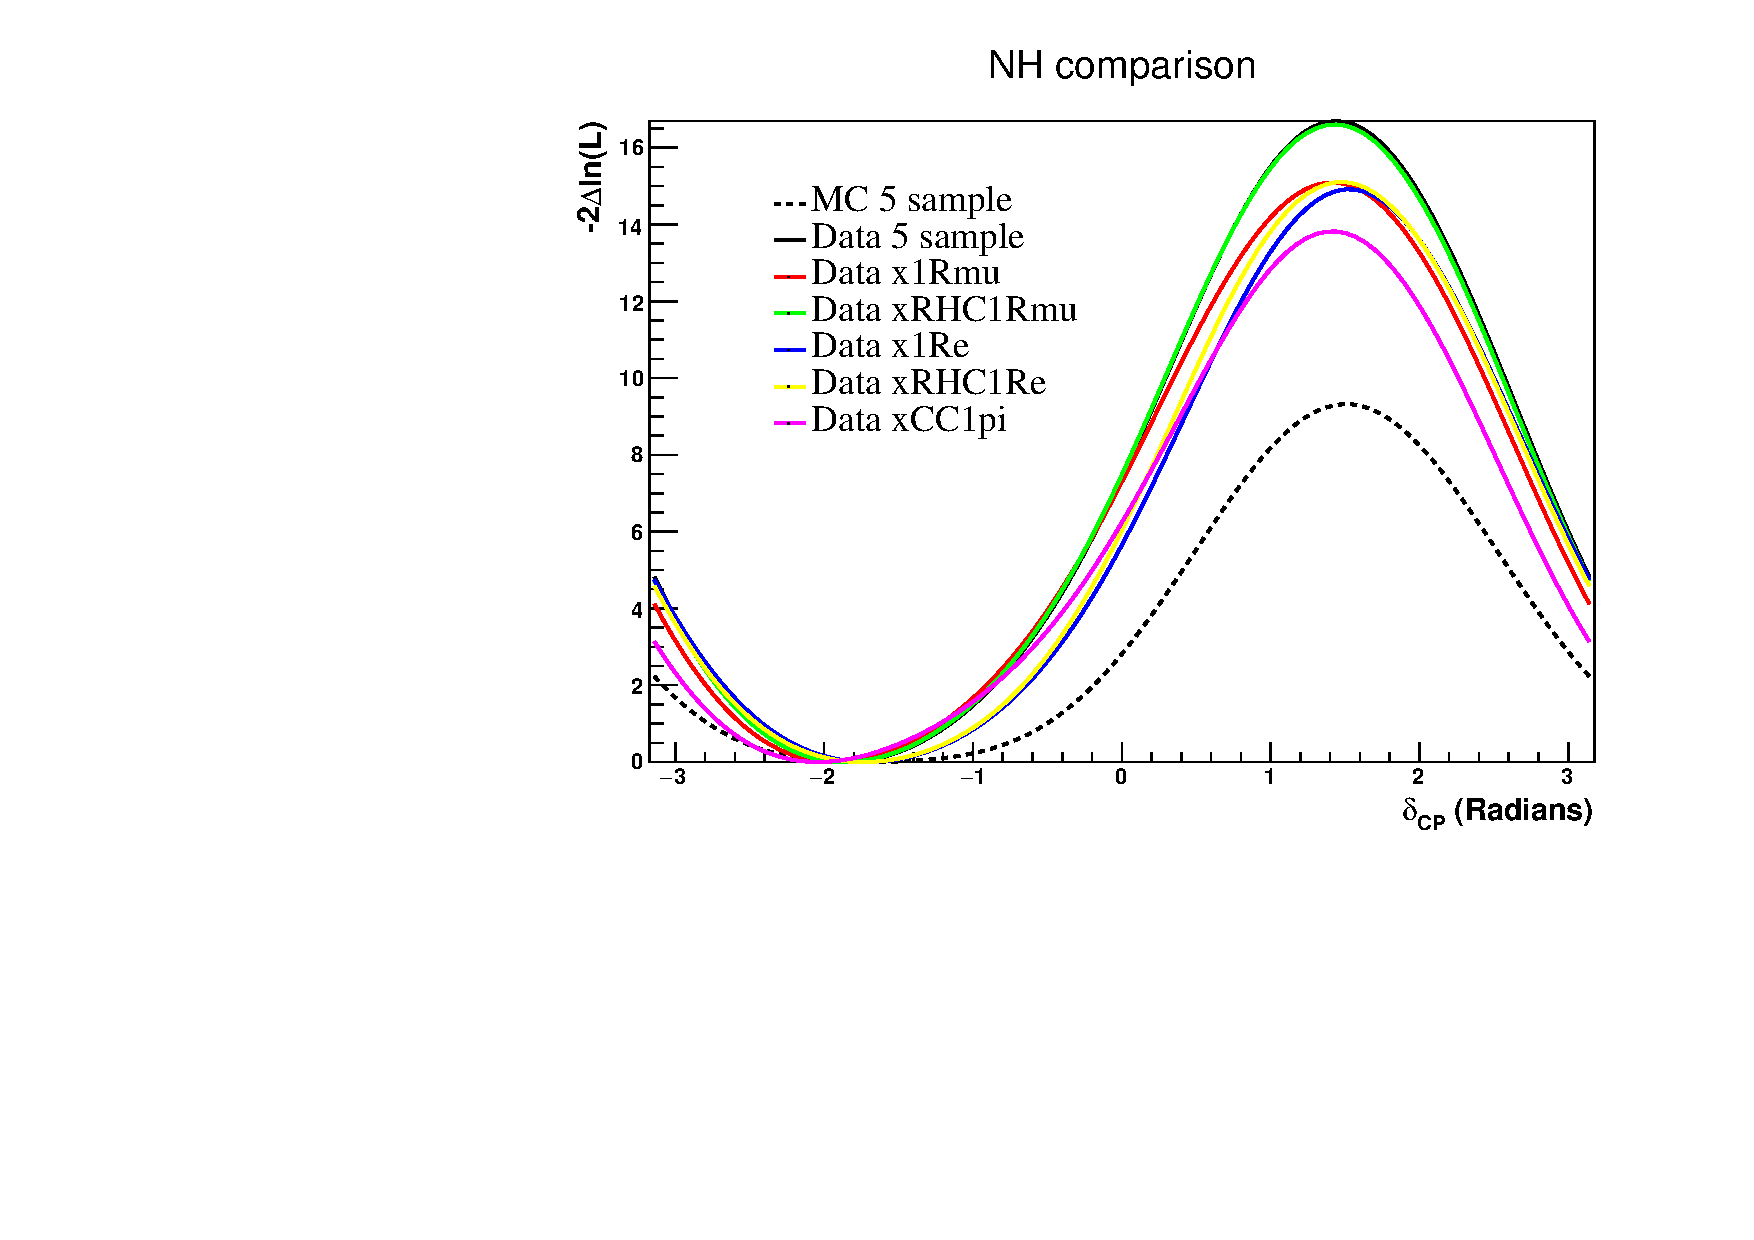
\includegraphics[width=0.9\textwidth]{studies/hybrids/deltacp_hybrids}
	\caption {
		The expected $\Delta\chi^2$ distribution as a function of \deltacp with reactor constraint for MC, data and data/MC hybrid data sets.
	}
	\label{fig:deltacp_hybrids}
\end{figure*}

A stronger than expected constraint is also evident in the disappearance contour, with greater exclusion in \ssqthtwothree. Similarly to the \deltacp hybrid fits above, \cref{fig:disappearance_hybrids} shows the expected sensitivity from the Asimov A data set (red), the data fit (black) and then a number of additional fits where one of the data samples was replaced by the corresponding Asimov A sample. From this one can see that the stronger constraint can be explained by the deficit in the observed number of events in the one-ring $\mu$-like sample.

\begin{figure*}[htb]
	\center
	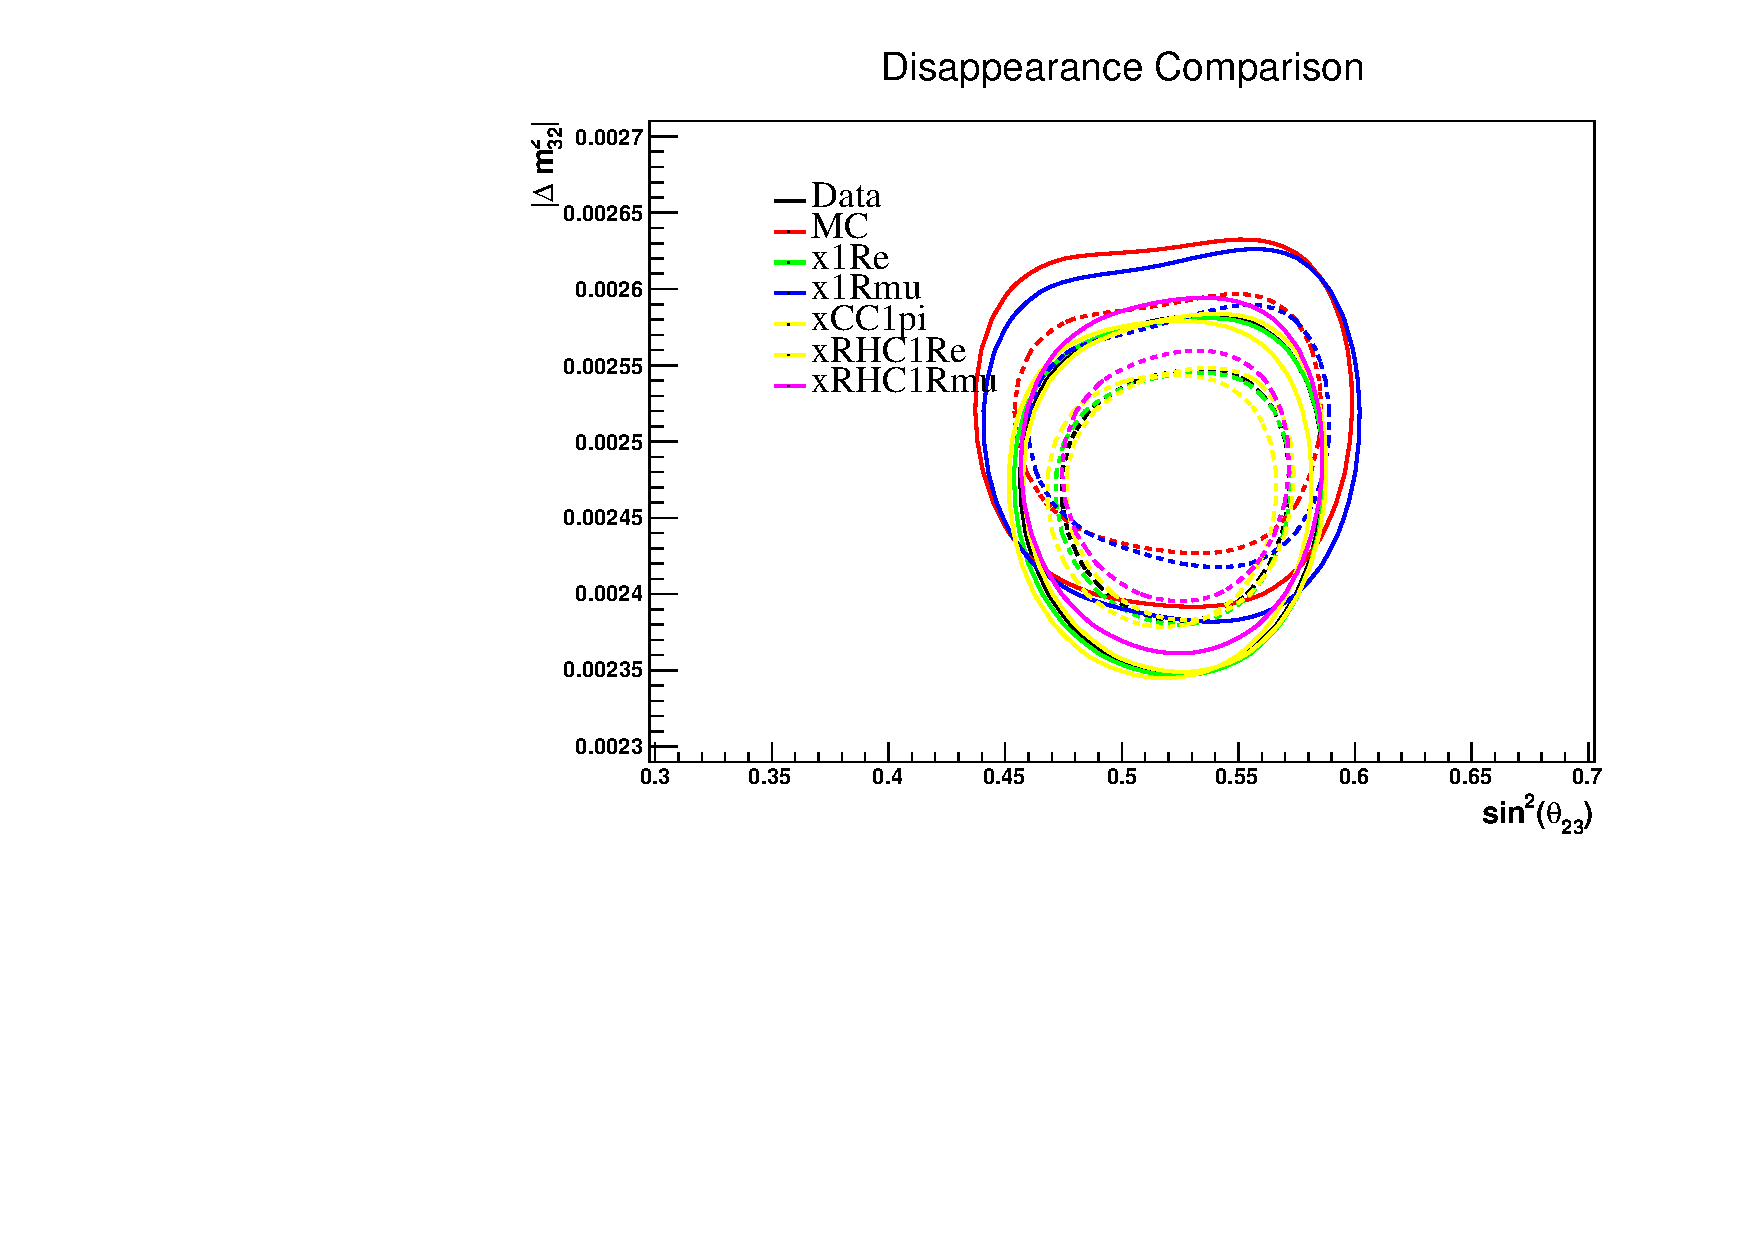
\includegraphics[width=0.9\textwidth]{studies/hybrids/disappearance_hybrids}
	\caption {
		The expected disappearance contours with reactor constraint for normal hierarchy for MC, data and data/MC hybrid data sets.
	}
	\label{fig:disappearance_hybrids}
\end{figure*}
\fi

\subsection {Comparison of \deltacp versus mass hierarchy result with sensitivity}
\label{sec:results:brazilian}

In order to provide a better understanding of the results of the \RunPeriod data fit, the result has been compared with the expected sensitivity obtained from a large number (10k) of toy experiments for different true values of \deltacp ($-\pi/2$ and the best fit value $-1.822$) and the mass hierarchy. The method used to determine the expected sensitivity is described in section 5.9 of \cite{OurRun18JointAnalysis3Flavour}.

\subsubsection{$\delta_{CP} = -\pi/2$ - normal hierarchy}

In \cref{fig:brazilian_dcp_mpi2} the \RunPeriod data result for \deltacp versus mass hierarchy is compared to the $1\sigma$ and $2\sigma$ uncertainties on the $\Delta\chi^2$ distributions corresponding to $\delta_{CP} = -\pi/2$, the top row includes one-sided distributions, the middle row two-sided distributions, with normal hierarchy on the left and inverted hierarchy on the right. We see that the data contour is contained within the one-sided $2\sigma$ band for inverted hierarchy, whilst the data contour falls just outside the $2\sigma$ band for normal hierarchy in the region around $\delta_{CP} = 0$, whereas the data contour is contained within the two-sided $2\sigma$ band in both hierarchies.

We also see an interesting feature near $\delta_{CP} = -\pi/2$ where the $\Delta\chi^2$ values have a wider distribution. This is due to the boundary at $\delta_{CP} = -\pi/2$ which causes a wider distribution when the parameter \deltacp would like to be pushed beyond the boundary in the fit.

Finally from \cref{fig:brazilian_dcp_mpi2}(c) we see that $\delta_{CP} = 0$ and $\delta_{CP} = \pi$ are excluded at 90\% confidence level in around 40-42\% (see \cref{tab:exclusion_prob}) of the toy experiments and excluded at $2\sigma$ confidence level in 27-29\% of the toy experiments.

\begin{figure*}[htb]
	\center
	\begin{subfigure}[b]{0.49\textwidth}
		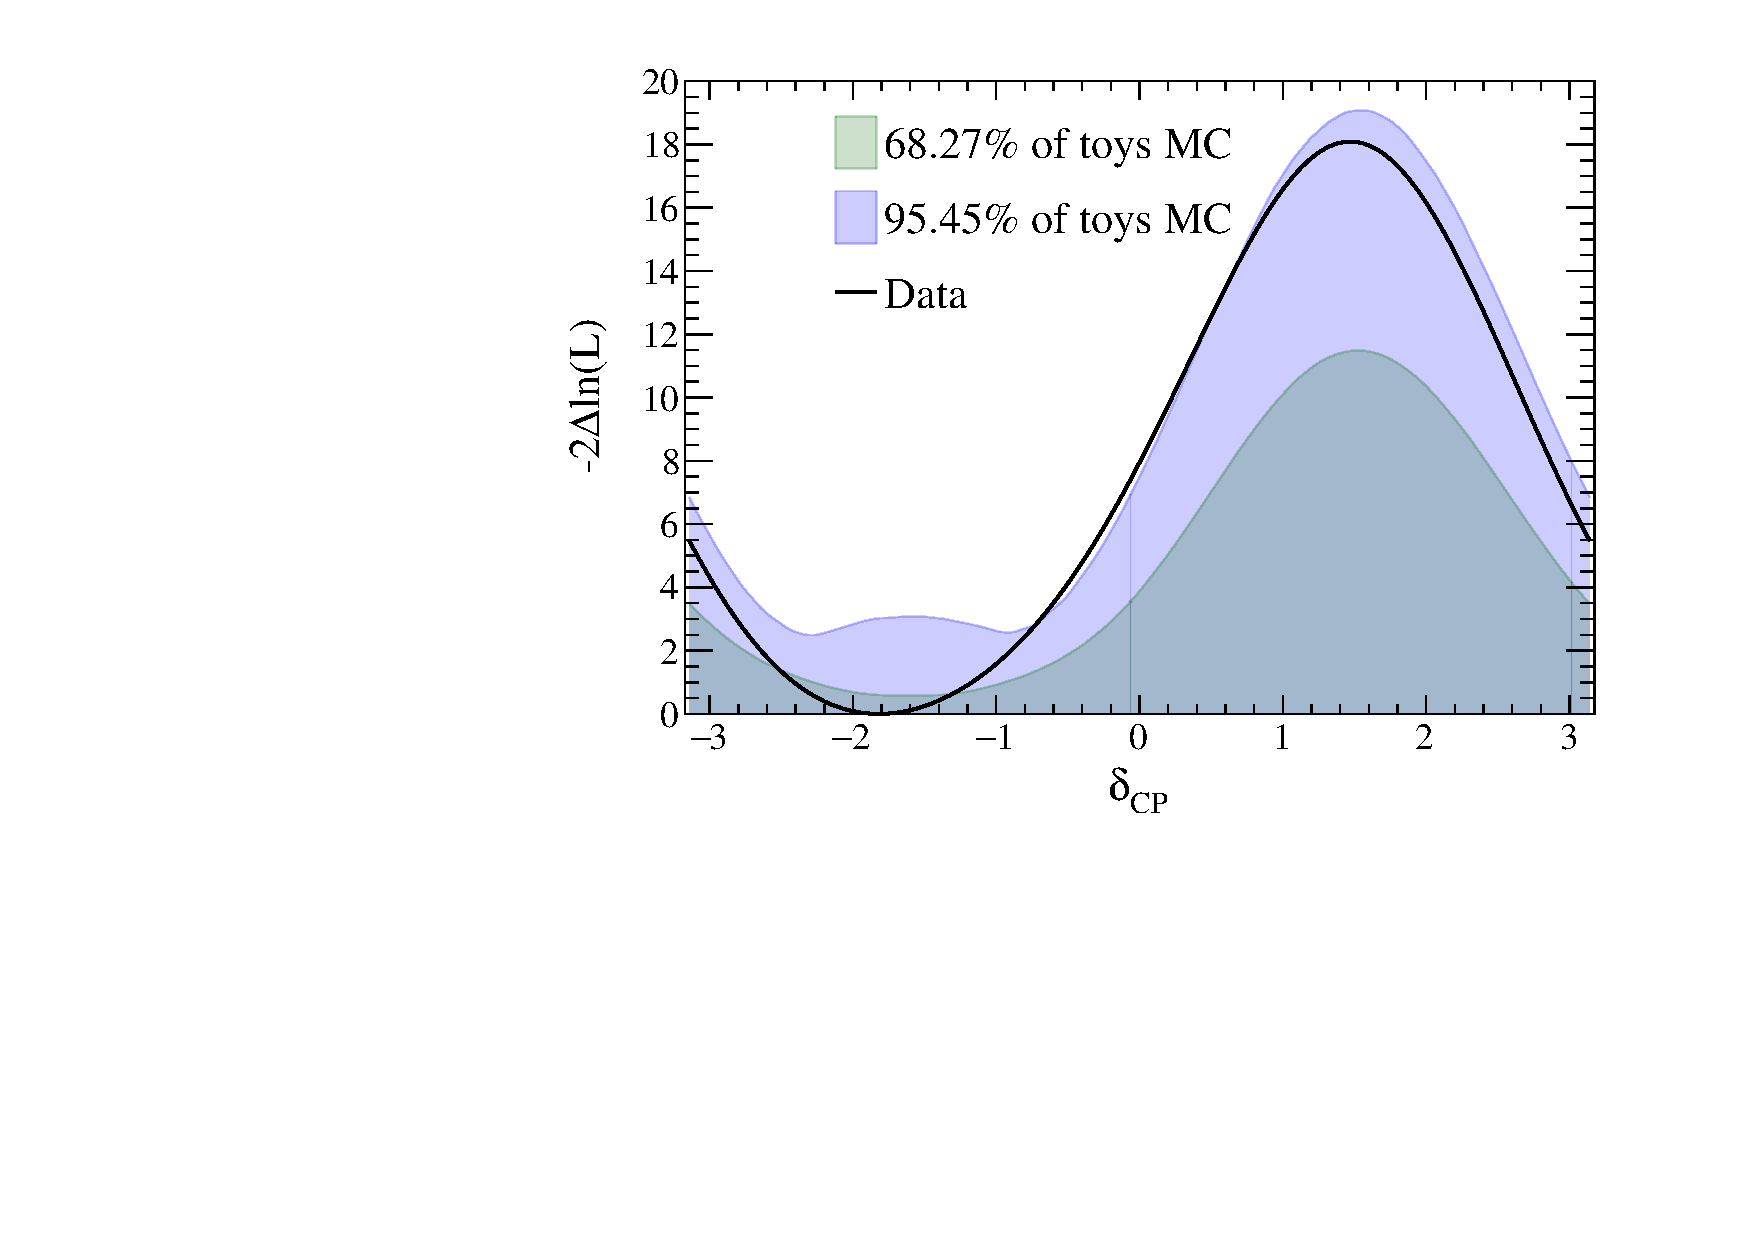
\includegraphics[width=0.9\textwidth]{images/fc/deltacp_mpi2_onesided_brazilian_nh}
		\caption{Normal hierarchy}
	\end{subfigure}
	\begin{subfigure}[b]{0.49\textwidth}
		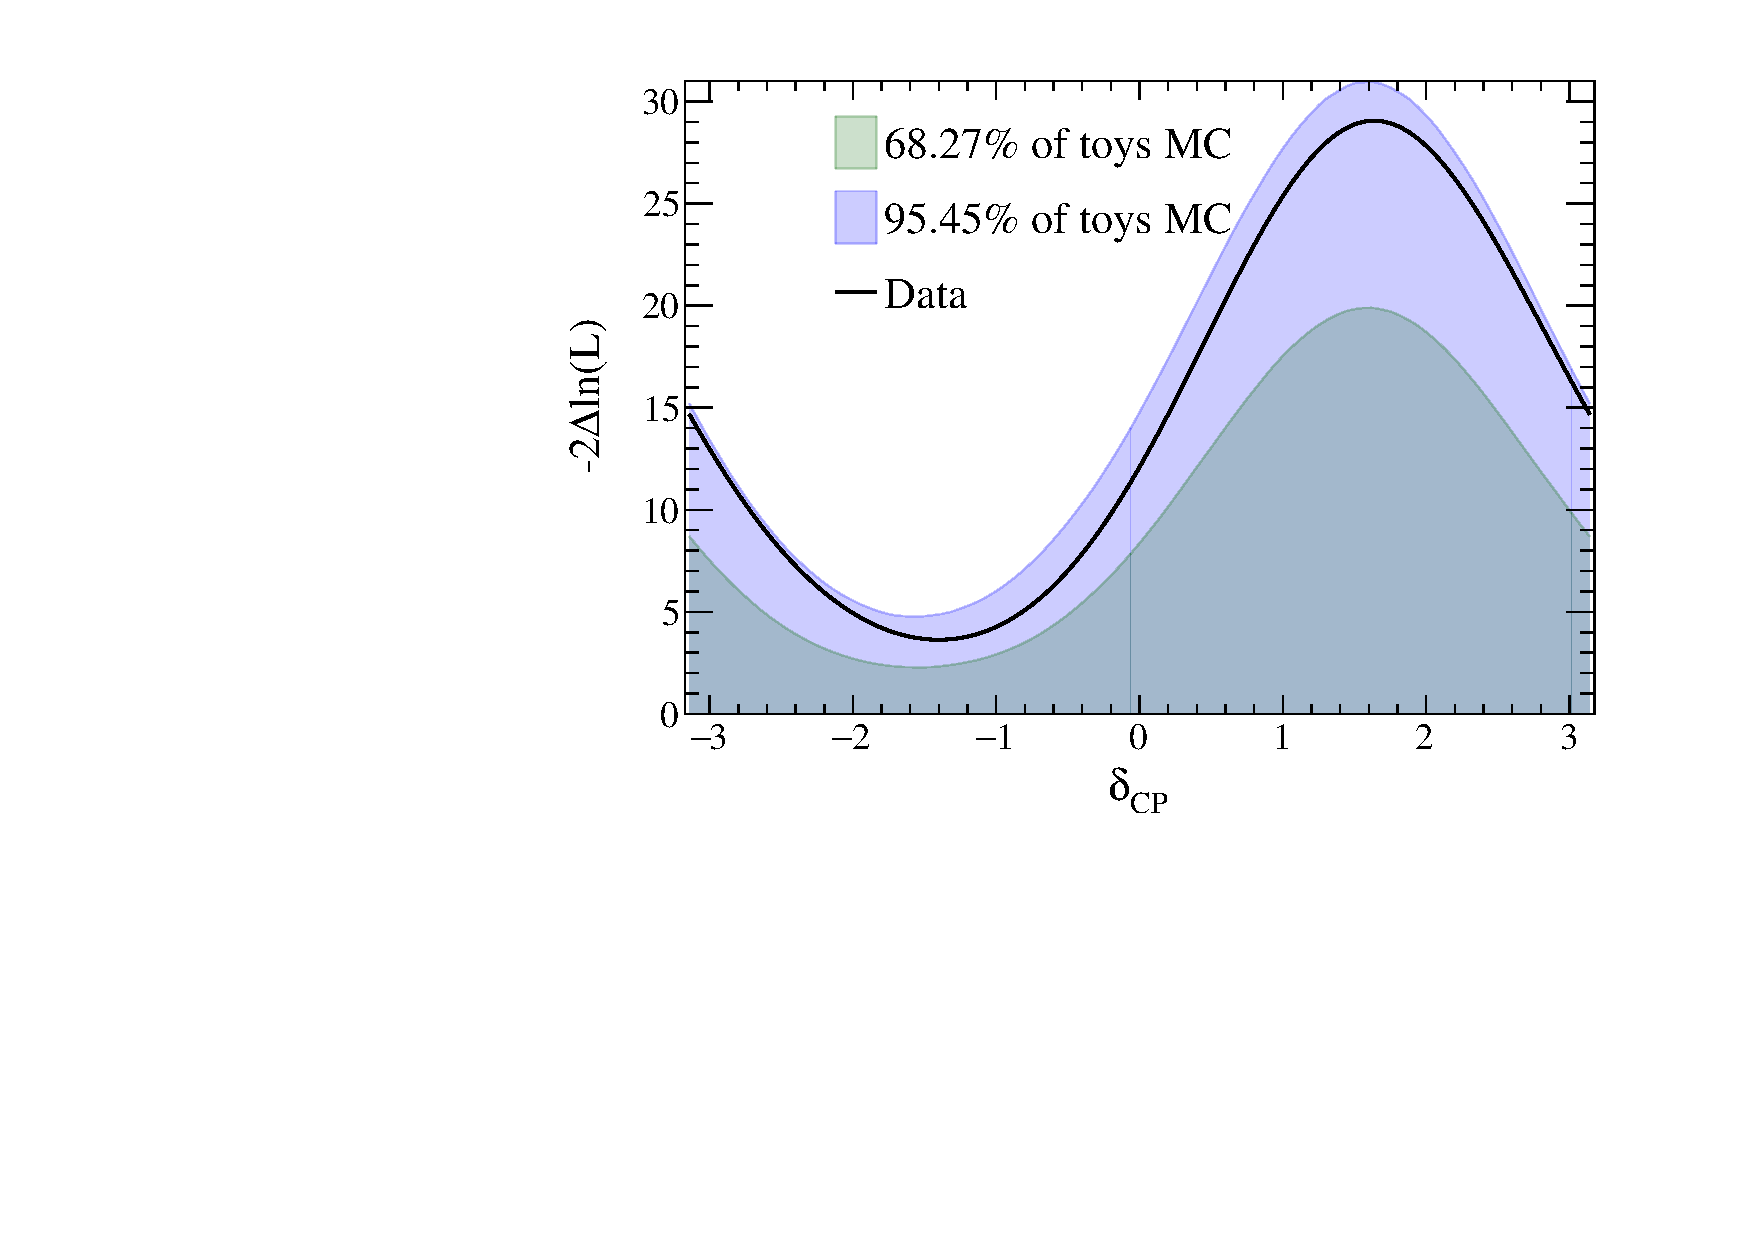
\includegraphics[width=0.9\textwidth]{images/fc/deltacp_mpi2_onesided_brazilian_ih}
		\caption{Inverted hierarchy}
	\end{subfigure}
	\begin{subfigure}[b]{0.49\textwidth}
		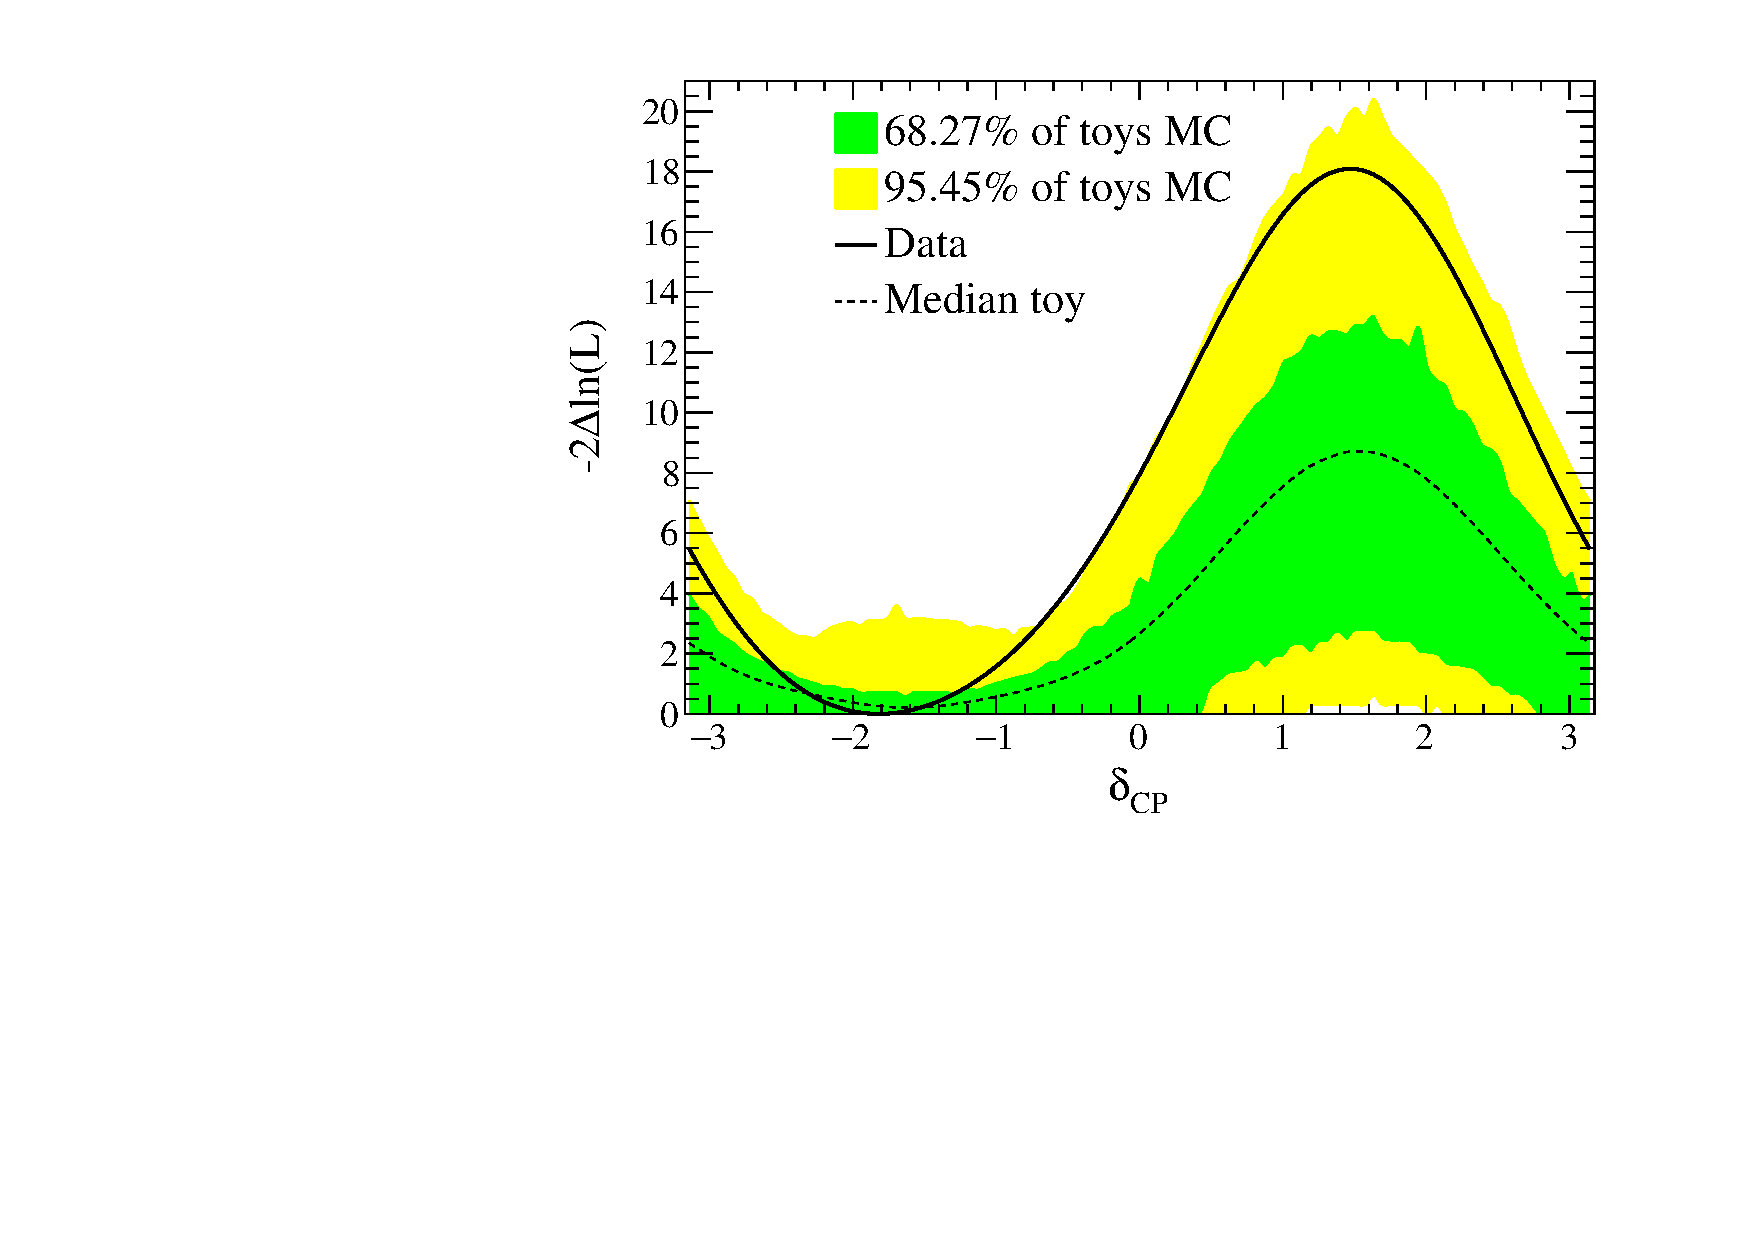
\includegraphics[width=0.9\textwidth]{images/fc/deltacp_mpi2_twosided_brazilian_nh}
		\caption{Normal hierarchy}
	\end{subfigure}
	\begin{subfigure}[b]{0.49\textwidth}
		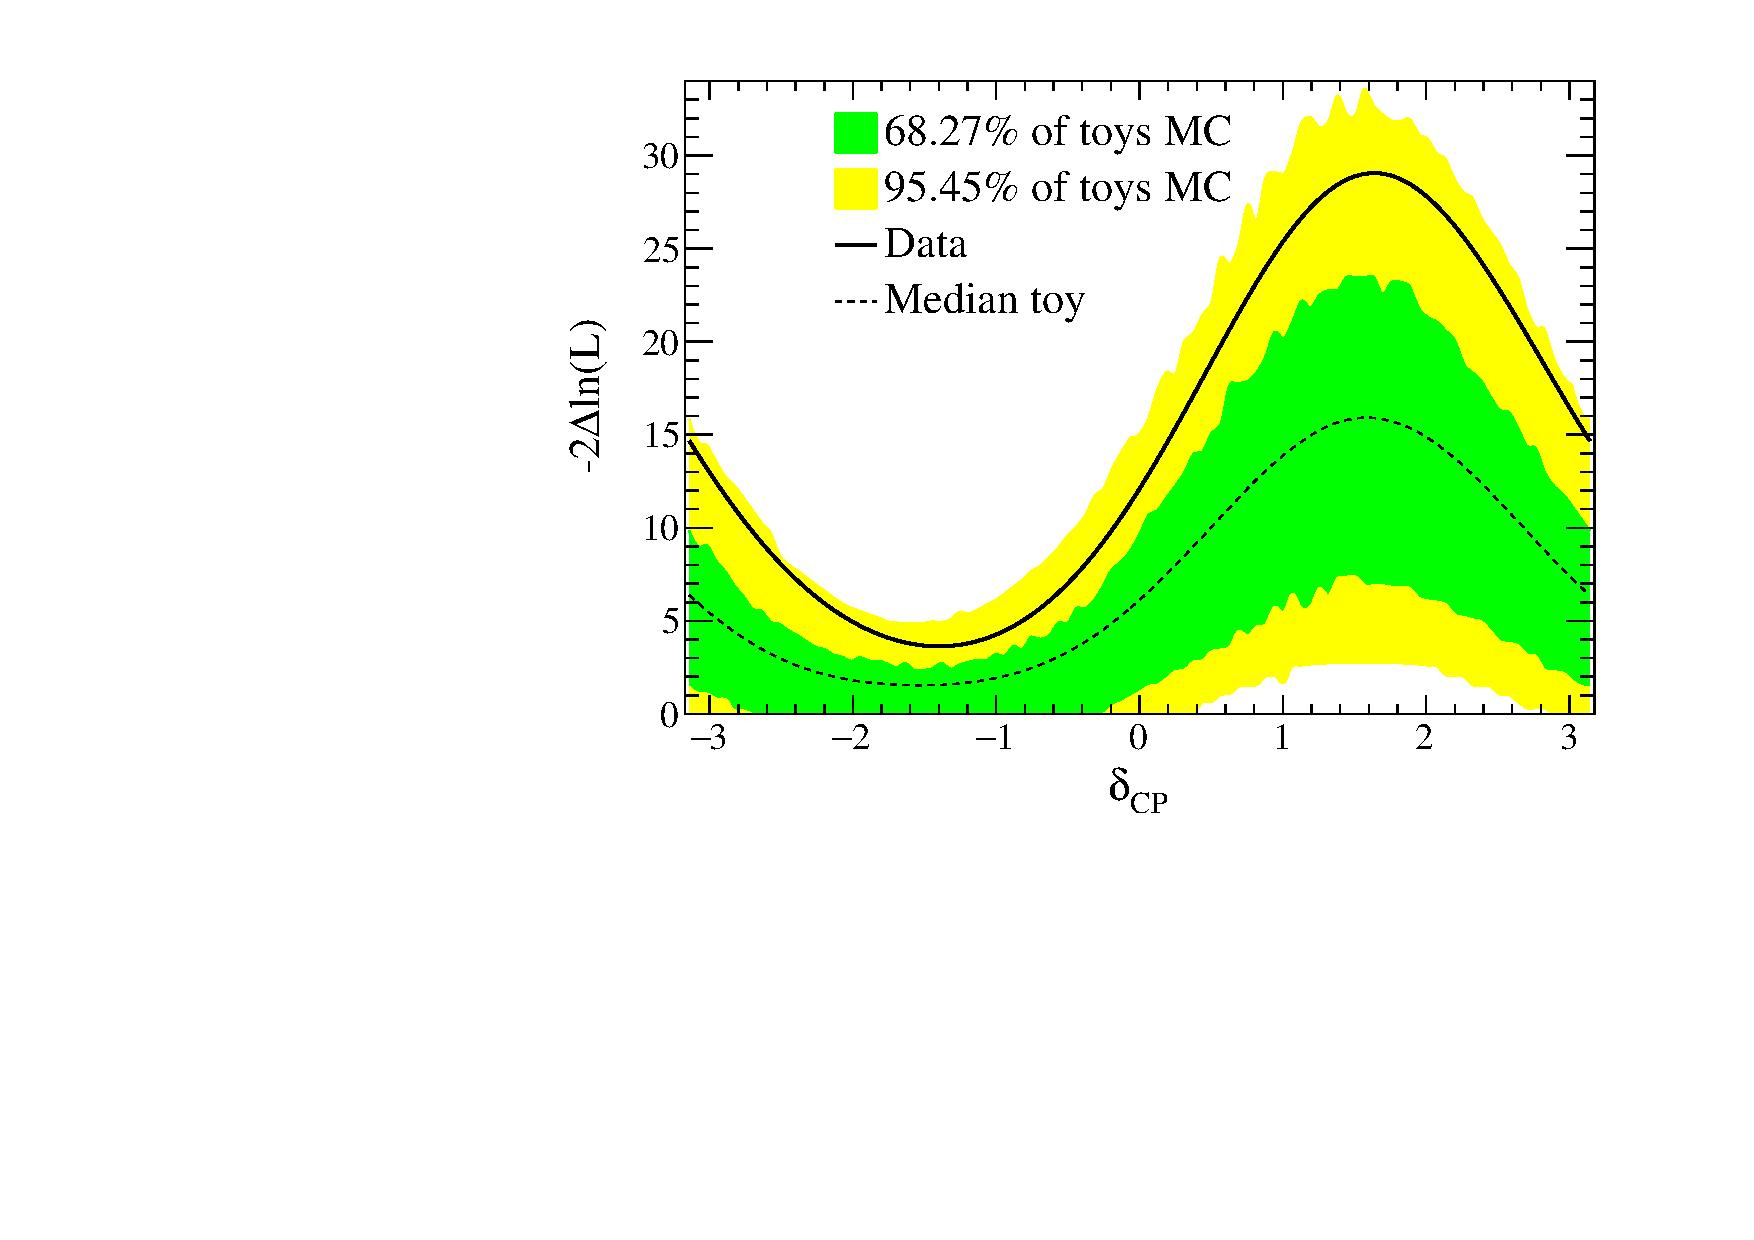
\includegraphics[width=0.9\textwidth]{images/fc/deltacp_mpi2_twosided_brazilian_ih}
		\caption{Inverted hierarchy}
	\end{subfigure}
	\begin{subfigure}[b]{0.49\textwidth}
		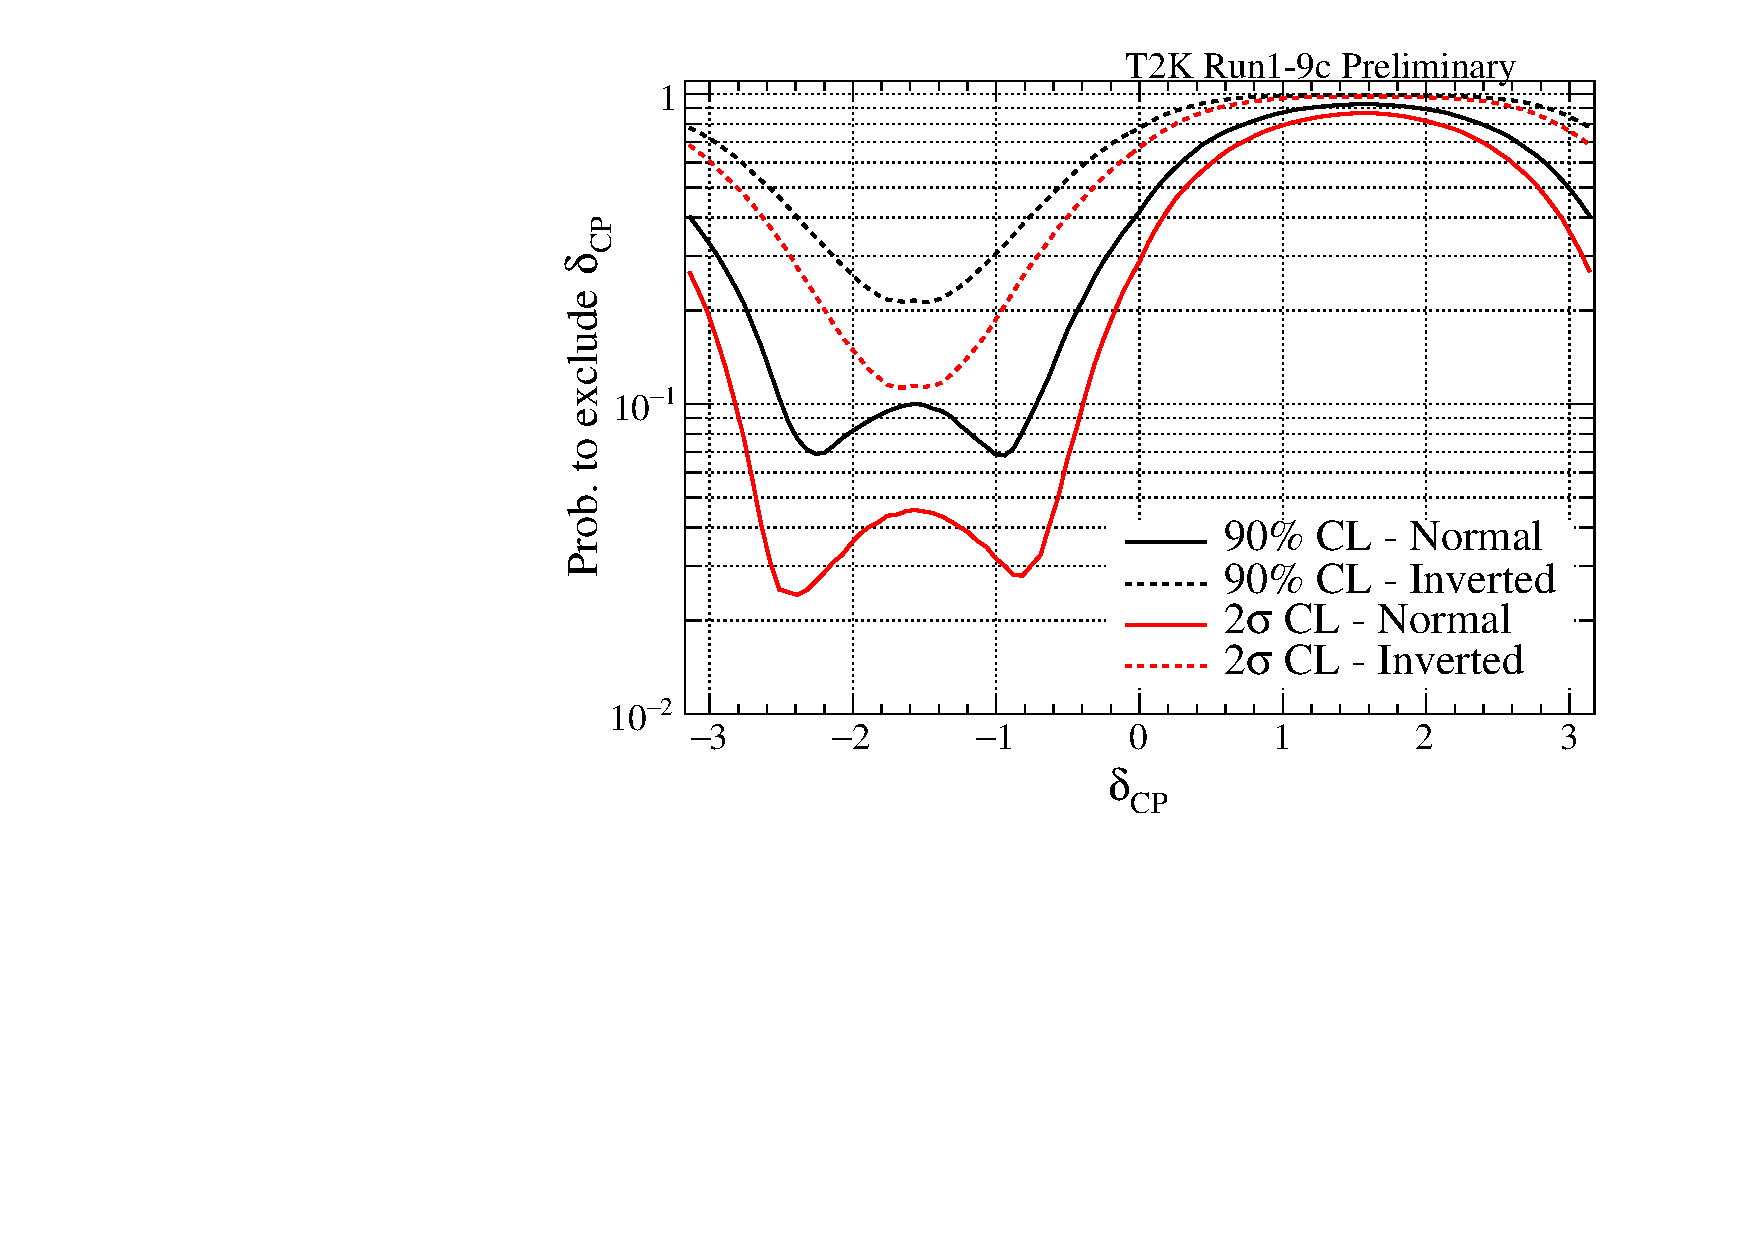
\includegraphics[width=0.9\textwidth]{images/fc/deltacp_mpi2_onesided_brazilian_prob_chisq}
		\caption{Data \(\Delta \chi^2\) probablility }
	\end{subfigure}
	\caption {
		The one-sided distribution of $\Delta\chi^2$ vs \deltacp obtained with \num{1e4} toy experiments generated with $\delta_{CP} = -\pi/2$ and normal hierarchy is shown. The $\Delta\chi^2$ distributions obtained by fixing the mass hierarchy to normal (left) and inverted (right) are shown, along with the $\Delta\chi^2$ values corresponding to 68.27\% and 95.45\% of the toy experiments and the average $\Delta\chi^2$ values from all experiments. Also shown are the fractions of toys which exclude each value of \deltacp to 90\% and $2\sigma$ using the Feldman-Cousins corrected critical values (bottom).
	}
	\label{fig:brazilian_dcp_mpi2}
\end{figure*}

\begin{table}[htb]
	\centering
	\begin{tabular}{| c | c | c | c |}
\hline
\deltacp & Hierarchy & 90\% & $2\sigma$ \\
\hline
0		& NH & 0.417 & 0.288 \\
$\pi$	& NH & 0.403 & 0.267 \\
0		& IH & 0.776 & 0.672 \\
$\pi$	& IH & 0.779 & 0.684 \\
\hline
\end{tabular}

	\caption{
		The fraction of toy experiments for which $\delta_{CP} = 0, \pi$ and normal and inverted hierarchy are excluded at 90\% and $2\sigma$ CL is shown. 10k toy experiments are used.
	}
	\label{tab:exclusion_prob}
\end{table}

\FloatBarrier

\subsubsection{$\delta_{CP} = -1.822$ - normal hierarchy}

In \cref{fig:brazilian_dcp_bf} the \RunPeriod data result for \deltacp versus mass hierarchy is compared to the $1\sigma$ and $2\sigma$ uncertainties on the $\Delta\chi^2$ distributions corresponding to $\delta_{CP} = -1.822$, the top row includes one-sided distributions, the middle row two-sided distributions, with normal hierarchy on the left and inverted hierarchy on the right. We see that the data contour is contained within the one-sided $2\sigma$ band for inverted hierarchy, whilst the data contour falls just outside the $2\sigma$ band for normal hierarchy in the region around $\delta_{CP} = 0$, whereas the data contour is contained within the two-sided $2\sigma$ band in both hierarchies.

Finally from \cref{fig:brazilian_dcp_bf}(c) we see that $\delta_{CP} = 0$ and $\delta_{CP} = \pi$ are excluded at 90\% confidence level in around 38-42\% (see \cref{tab:exclusion_prob}) of the toy experiments and excluded at $2\sigma$ confidence level in around 25-29\% of the toy experiments.

\begin{figure*}[htb]
	\center
	\begin{subfigure}[b]{0.49\textwidth}
		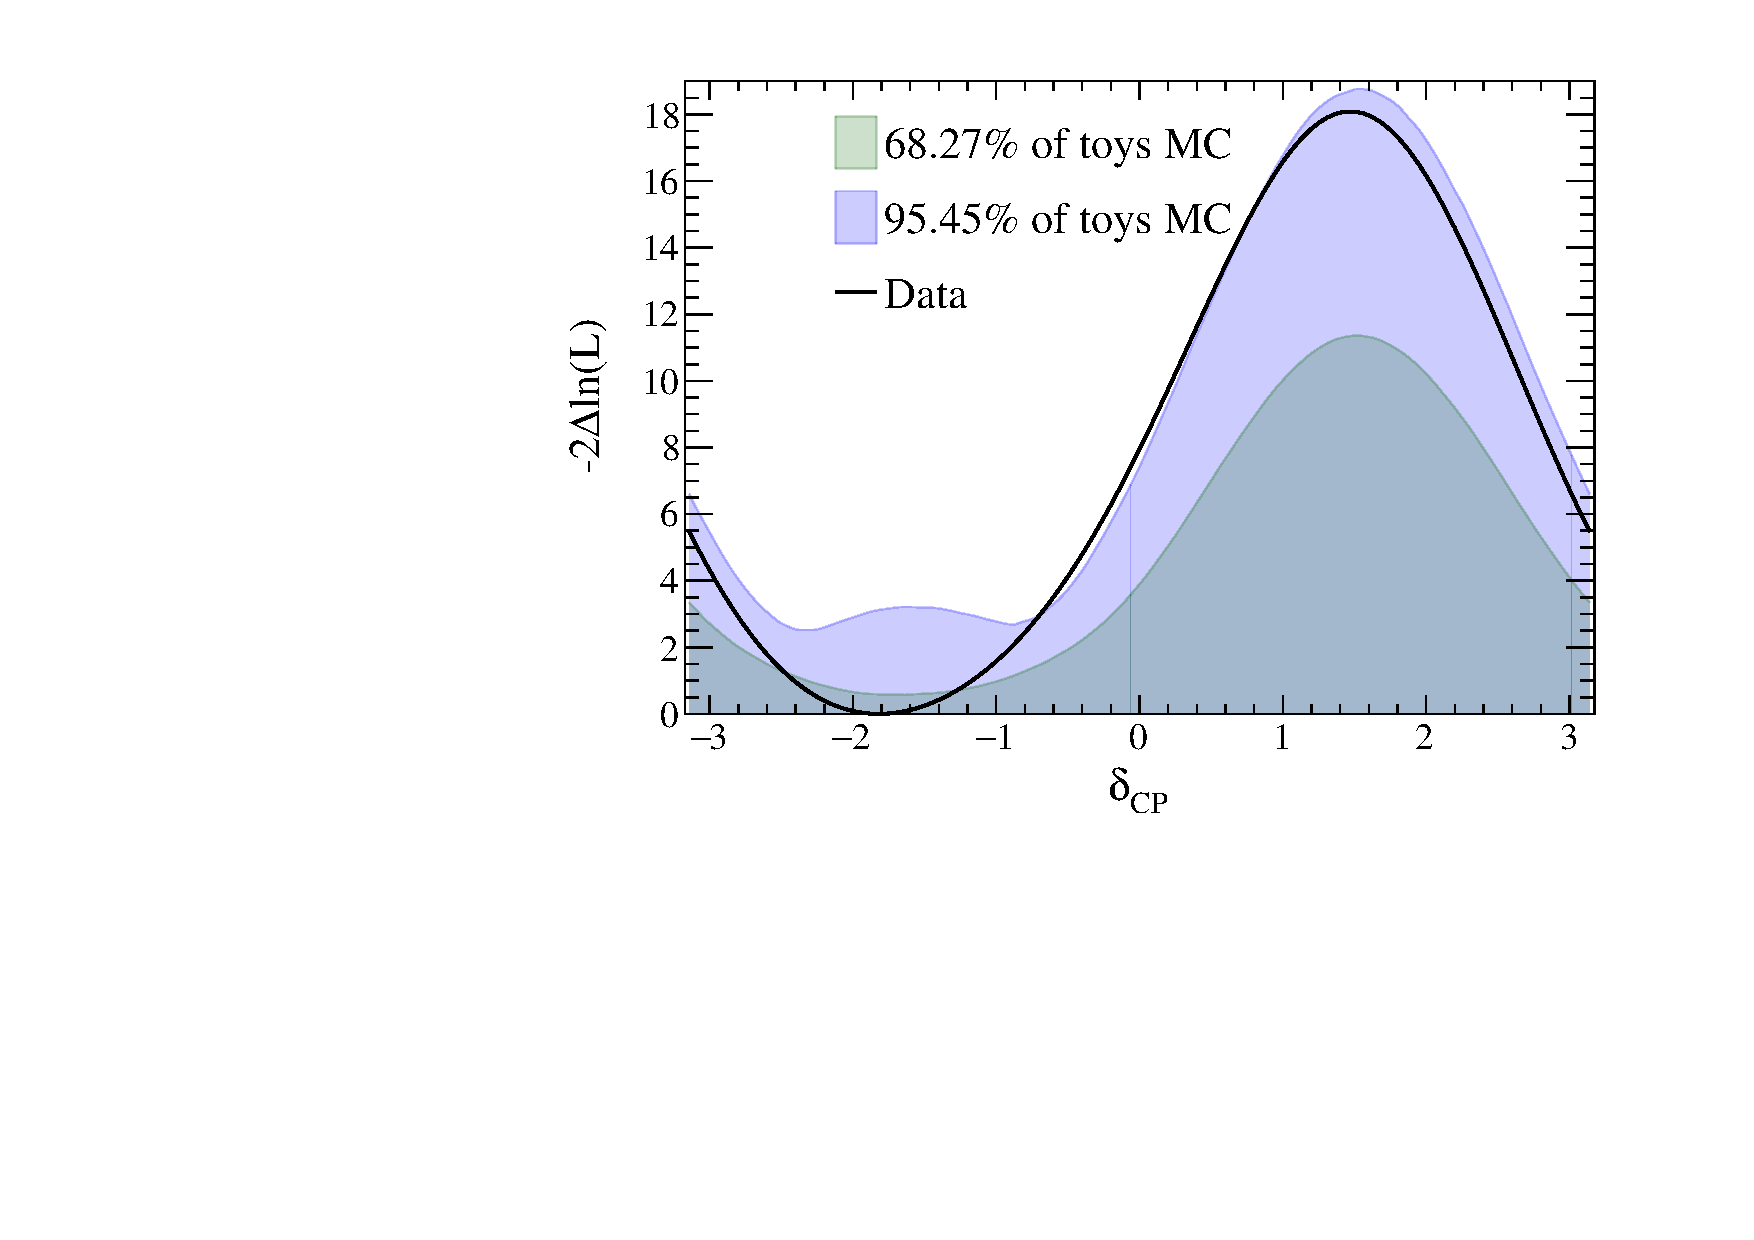
\includegraphics[width=0.9\textwidth]{images/fc/deltacp_bestfit_onesided_brazilian_nh}
		\caption{Normal hierarchy}
	\end{subfigure}
	\begin{subfigure}[b]{0.49\textwidth}
		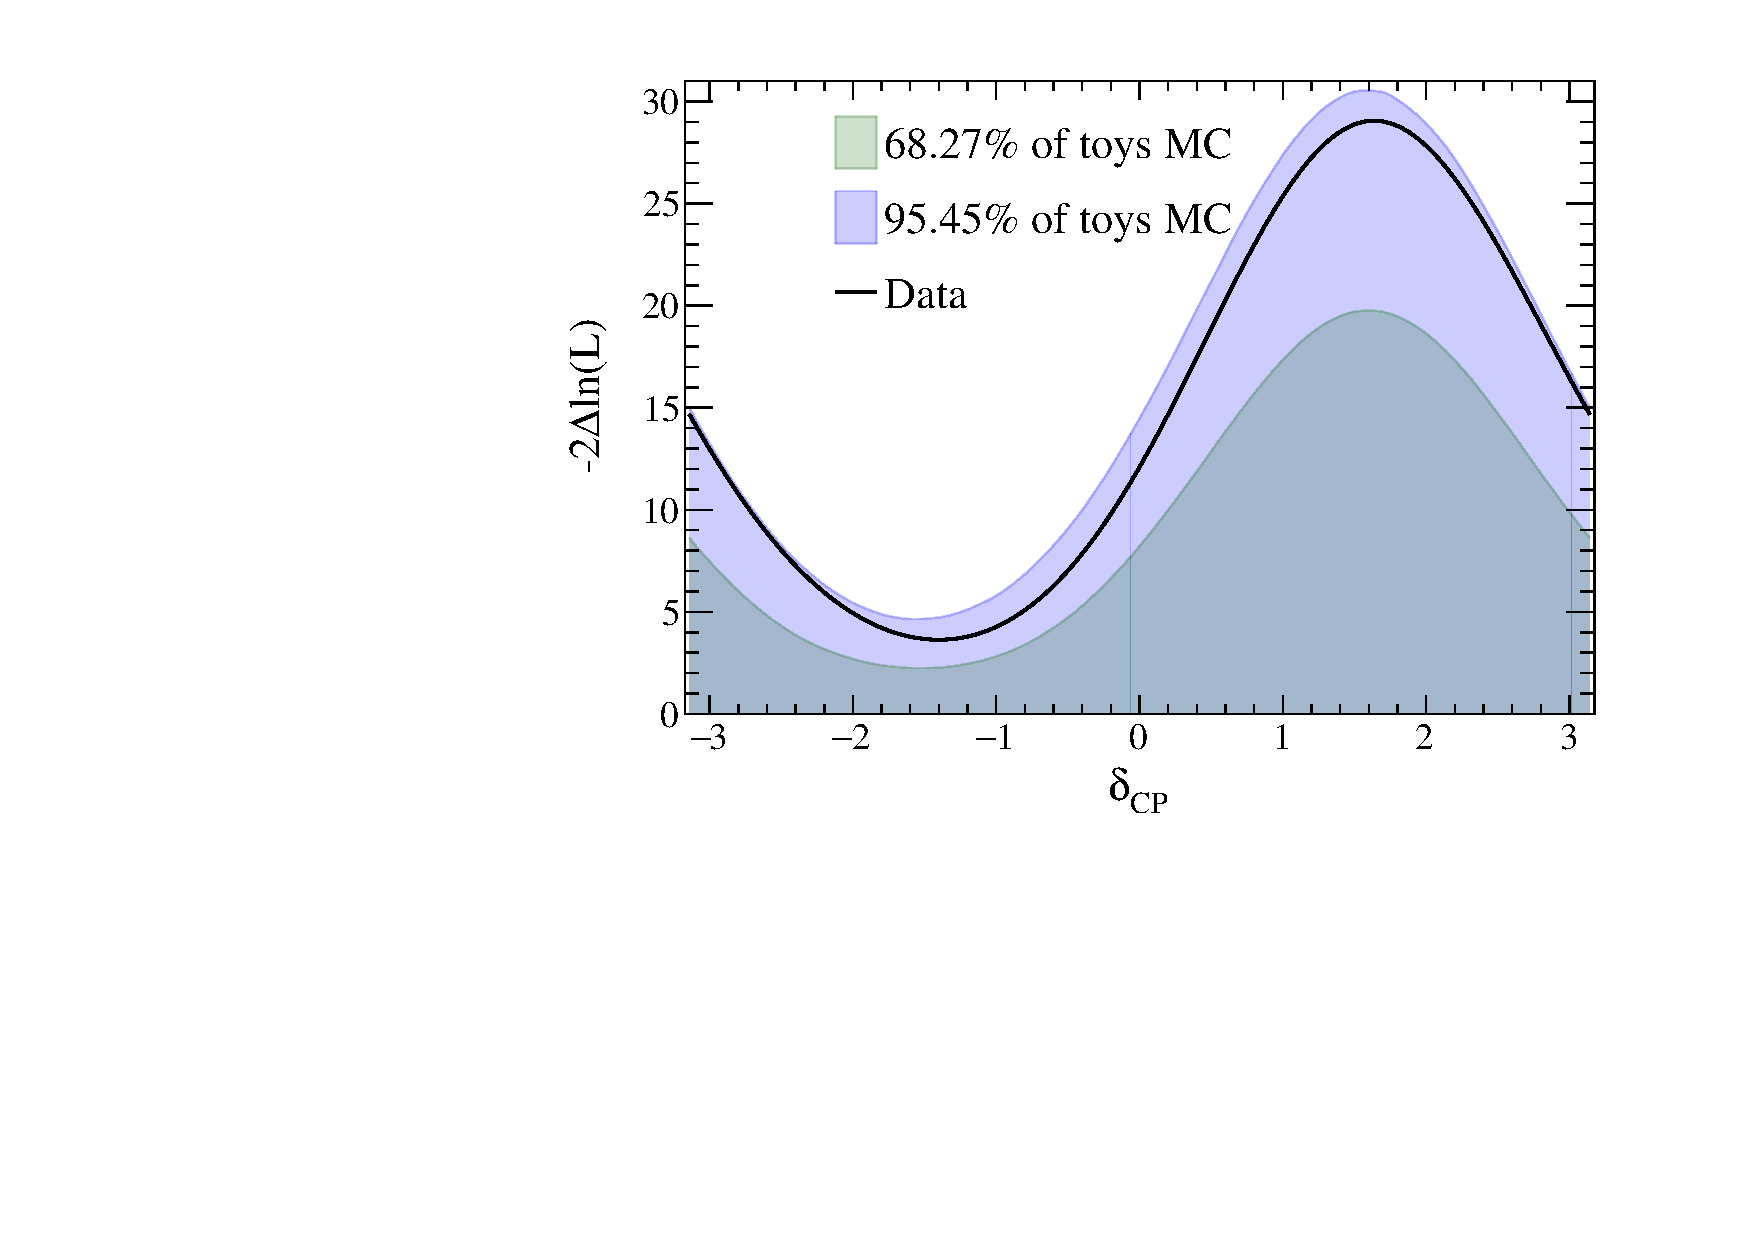
\includegraphics[width=0.9\textwidth]{images/fc/deltacp_bestfit_onesided_brazilian_ih}
		\caption{Inverted hierarchy}
	\end{subfigure}
	\begin{subfigure}[b]{0.49\textwidth}
		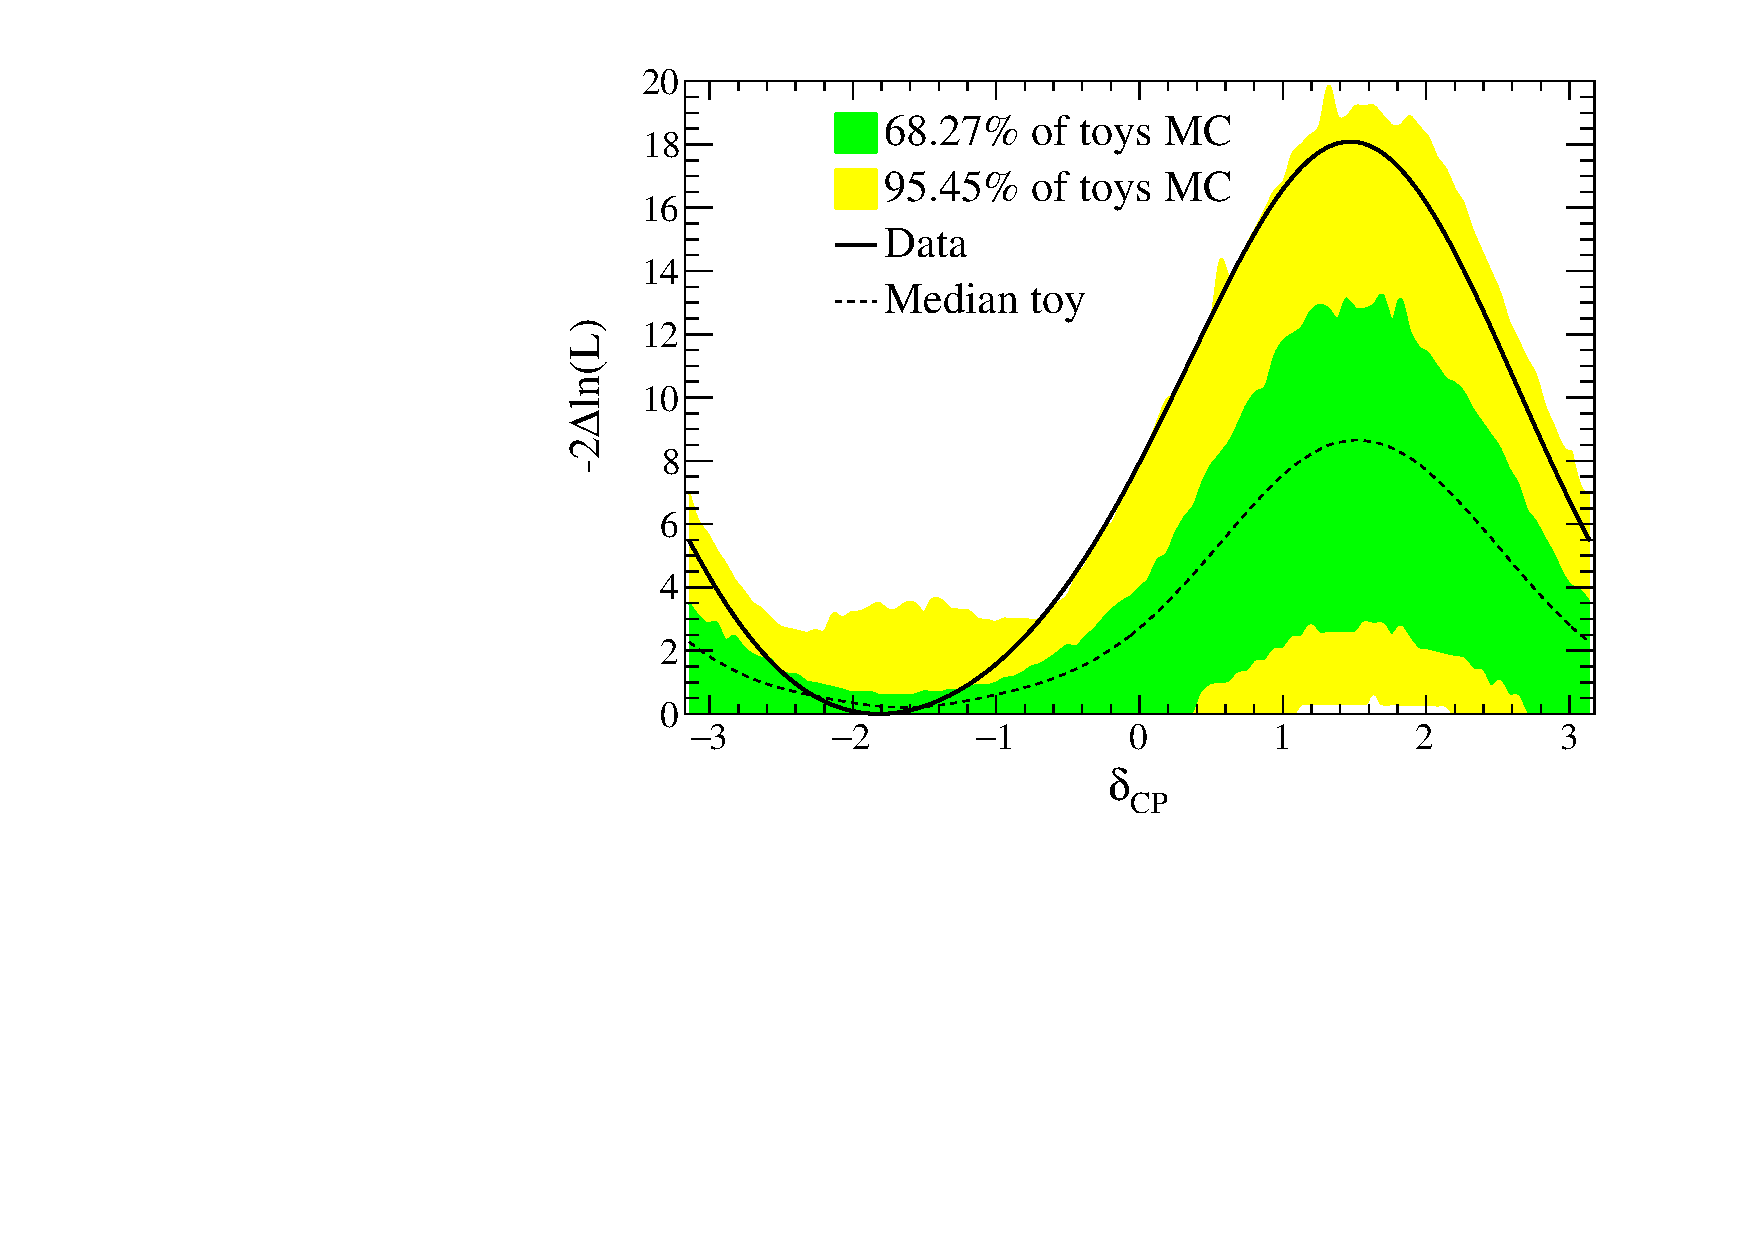
\includegraphics[width=0.9\textwidth]{images/fc/deltacp_bestfit_twosided_brazilian_nh}
		\caption{Normal hierarchy}
	\end{subfigure}
	\begin{subfigure}[b]{0.49\textwidth}
		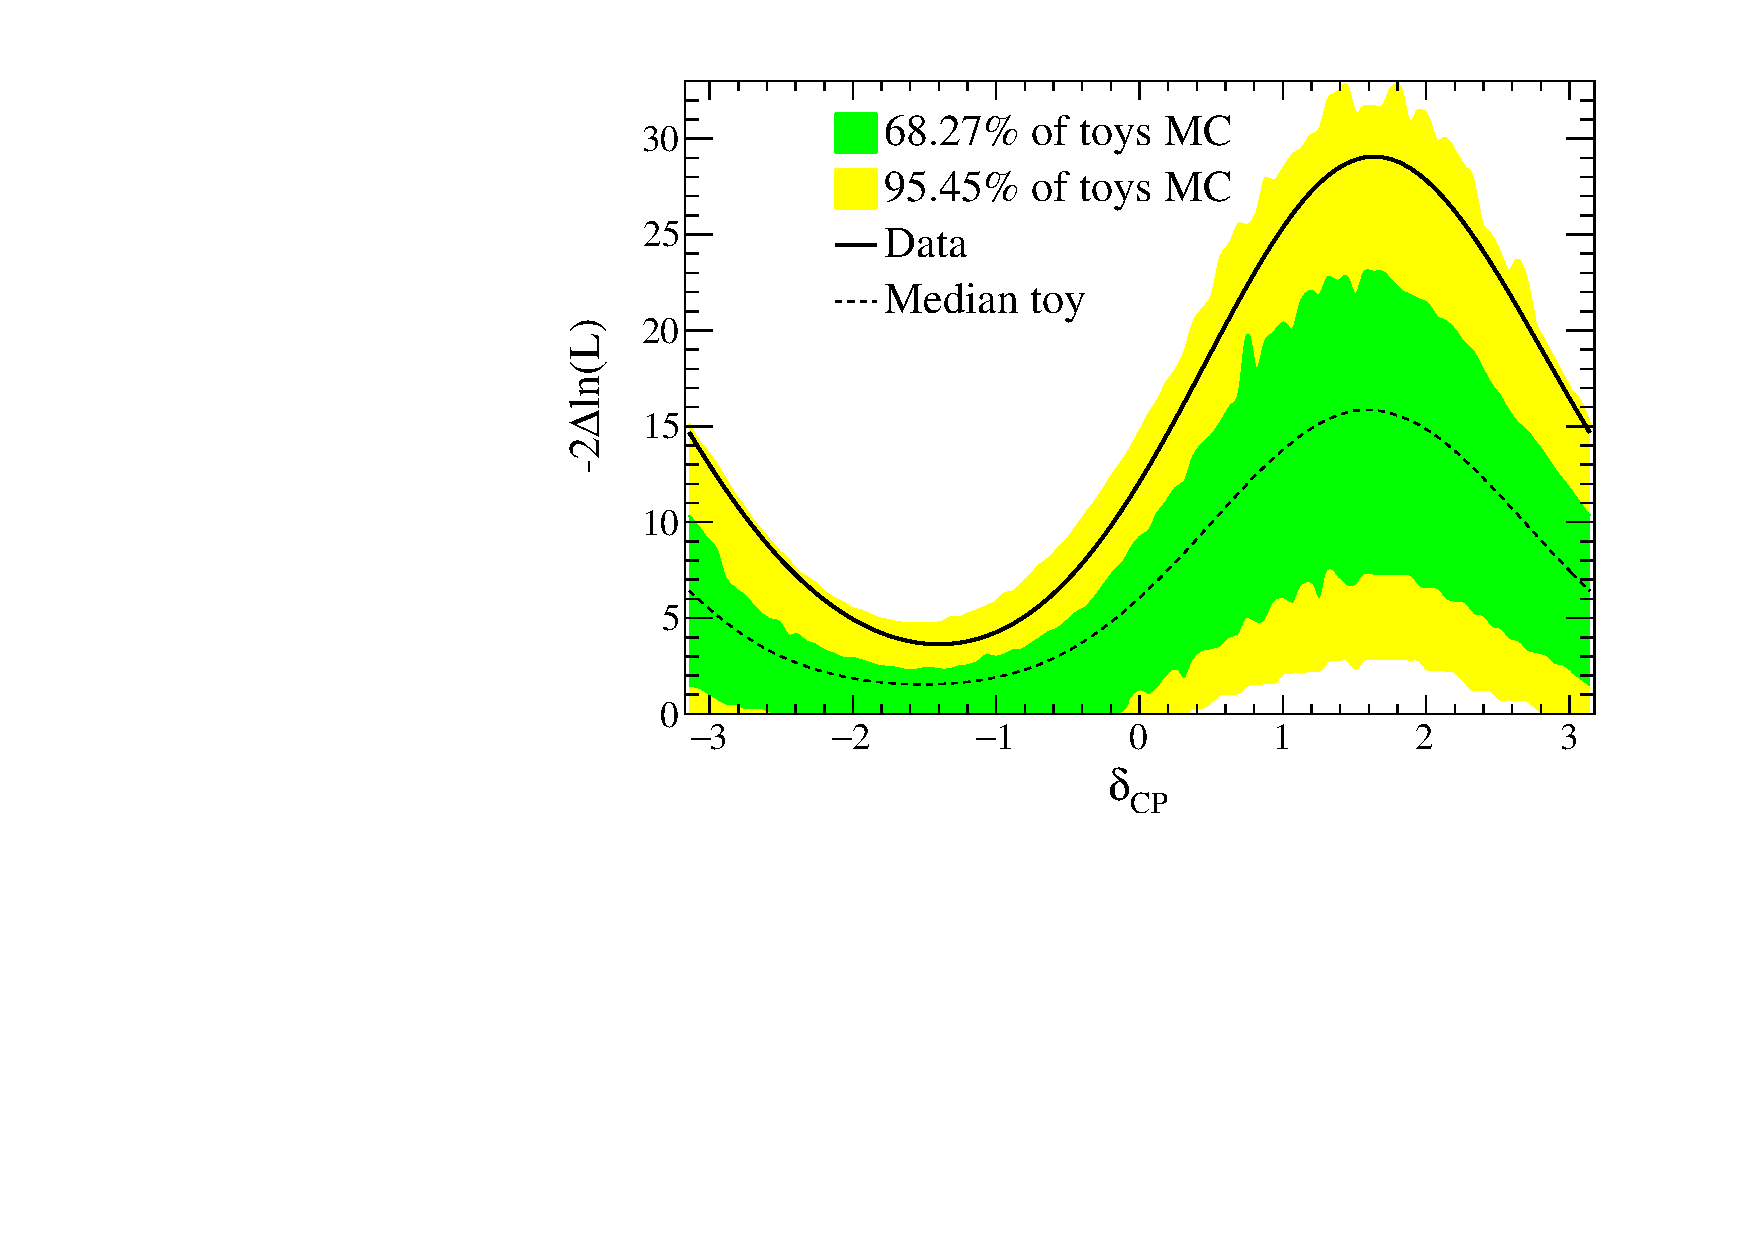
\includegraphics[width=0.9\textwidth]{images/fc/deltacp_bestfit_twosided_brazilian_ih}
		\caption{Inverted hierarchy}
	\end{subfigure}
	\begin{subfigure}[b]{0.49\textwidth}
		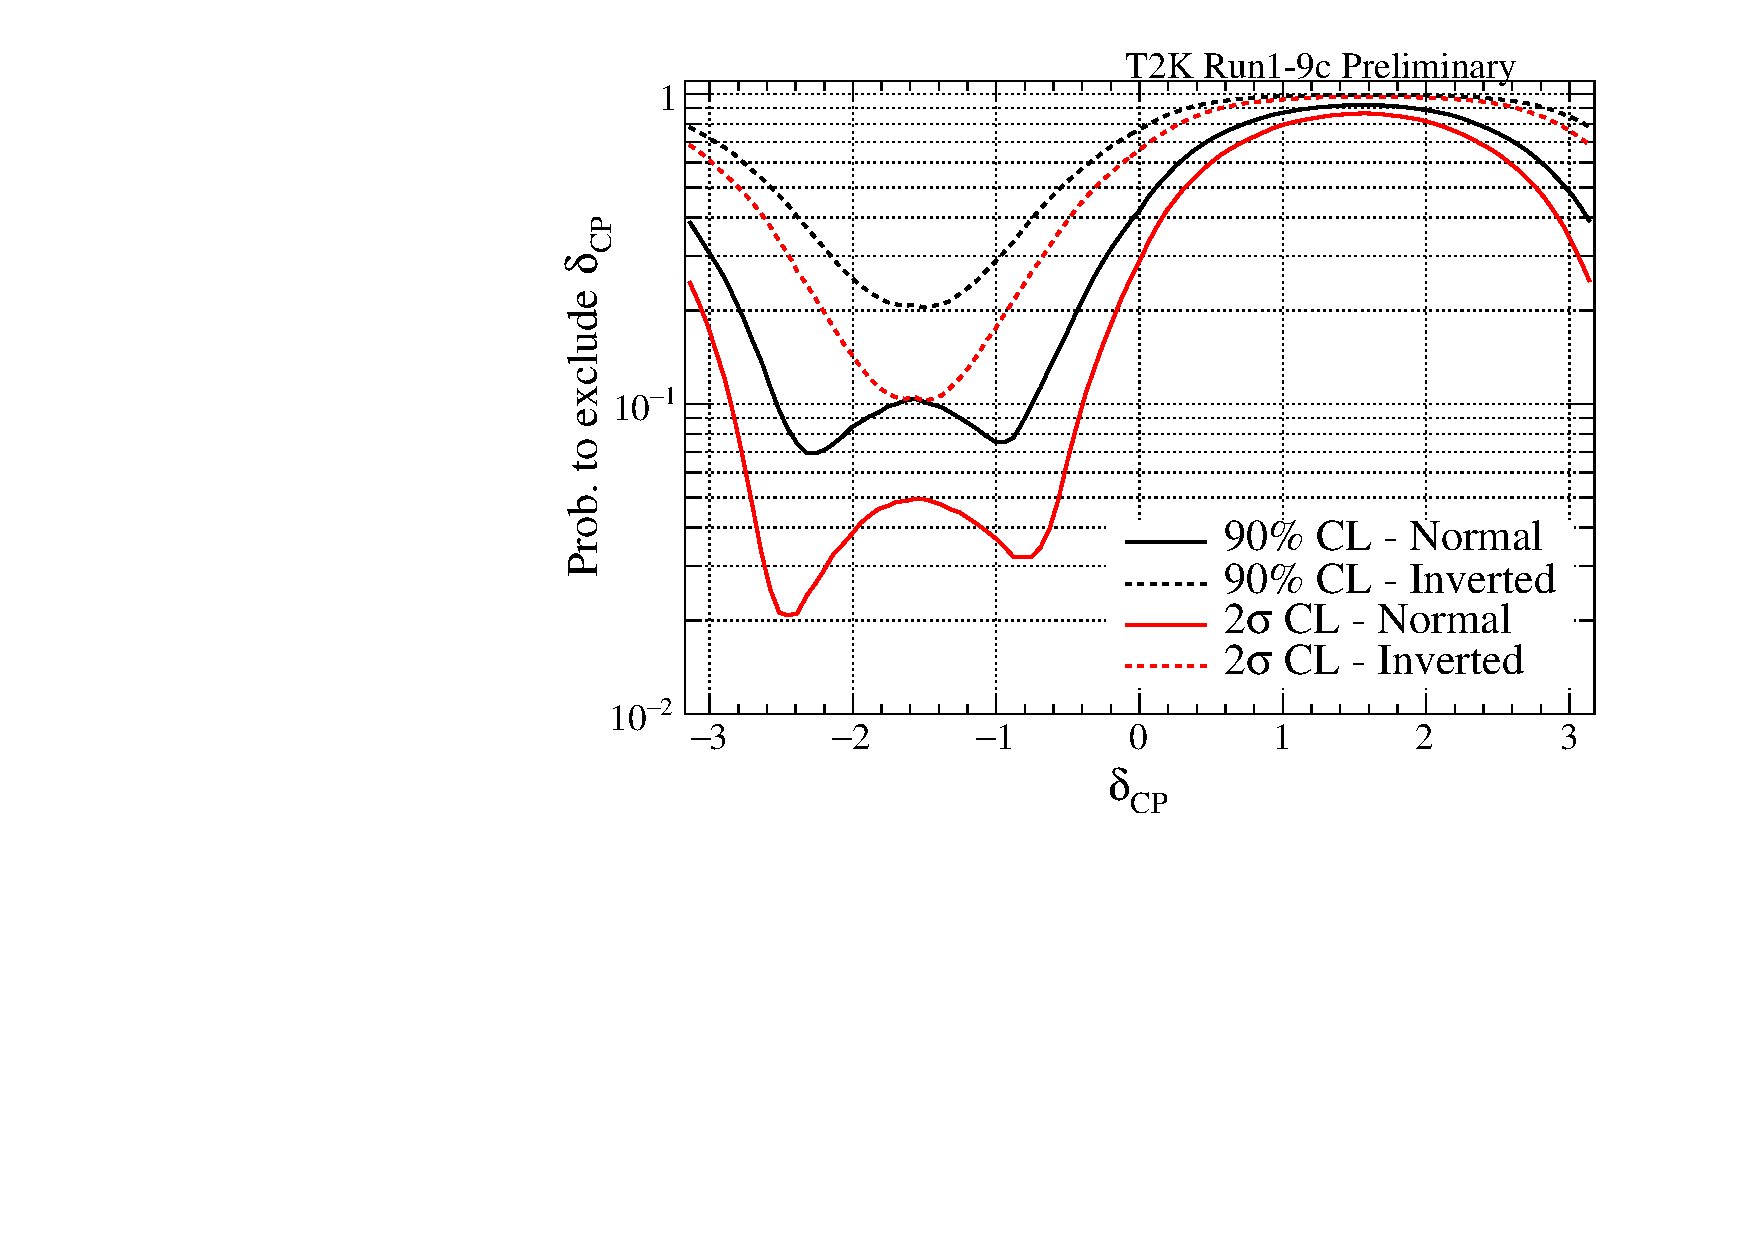
\includegraphics[width=0.9\textwidth]{images/fc/deltacp_bestfit_onesided_brazilian_prob_chisq}
		\caption{Data \(\Delta \chi^2\) probablility }
	\end{subfigure}
	\caption {
		The one-sided distribution of $\Delta\chi^2$ vs \deltacp obtained with \num{1e4} toy experiments generated with $\delta_{CP} = -1.822$ and normal hierarchy is shown. The $\Delta\chi^2$ distributions obtained by fixing the mass hierarchy to normal (left) and inverted (right) are shown, along with the $\Delta\chi^2$ values corresponding to 68.27\% and 95.45\% of the toy experiments and the average $\Delta\chi^2$ values from all experiments. Also shown are the fractions of toys which exclude each value of \deltacp to 90\% and $2\sigma$ using the Feldman-Cousins corrected critical values (bottom).
	}
	\label{fig:brazilian_dcp_bf}
\end{figure*}

\begin{table}[htb]
	\centering
	\begin{tabular}{| c | c | c | c |}
\hline
\deltacp & Hierarchy & 90\% & $2\sigma$ \\
\hline
0		& NH & 0.421 & 0.288 \\
$\pi$	& NH & 0.388 & 0.248 \\
0		& IH & 0.768 & 0.660 \\
$\pi$	& IH & 0.783 & 0.685 \\
\hline
\end{tabular}

	\caption{
		The fraction of toy experiments for which $\delta_{CP} = 0, \pi$ and normal and inverted hierarchy are excluded at 90\% and $2\sigma$ CL is shown. 10k toy experiments are used.
	}
	\label{tab:exclusion_prob_bf}
\end{table}

\FloatBarrier

\subsection {Comparison of $e$-like event rates with expectation}
\label{sec:results:bievent}

It is valuable to see how different values of \deltacp, \ssqthtwothree and hierarchy affect the predicted event rates. \Cref{fig:bievent} shows the predicted $\nueb$ event rate vs $\nue$ event rate for best-fit values of oscillation parameters where \deltacp is varied between CP conserving and maximally CP violating values, and \ssqthtwothree is varied around its best-fit, for both hierarchies. Event rates for a given value of \ssqthtwothree and mass hierarchy are linearly interpolated between those computed for 9 evenly-spaced values of \deltacp from $-\pi$ to $+\pi$ to indicate the behaviour produced by varying \deltacp. In addition the systematic, and systematic + statistical error contours are shown for the case of normal hierarchy, with $\delta_{CP} = -\pi/2$ and $\sin^2\theta_{23} = 0.5$ for 300K toy throws.

\begin{figure*}[htb]
	\center
	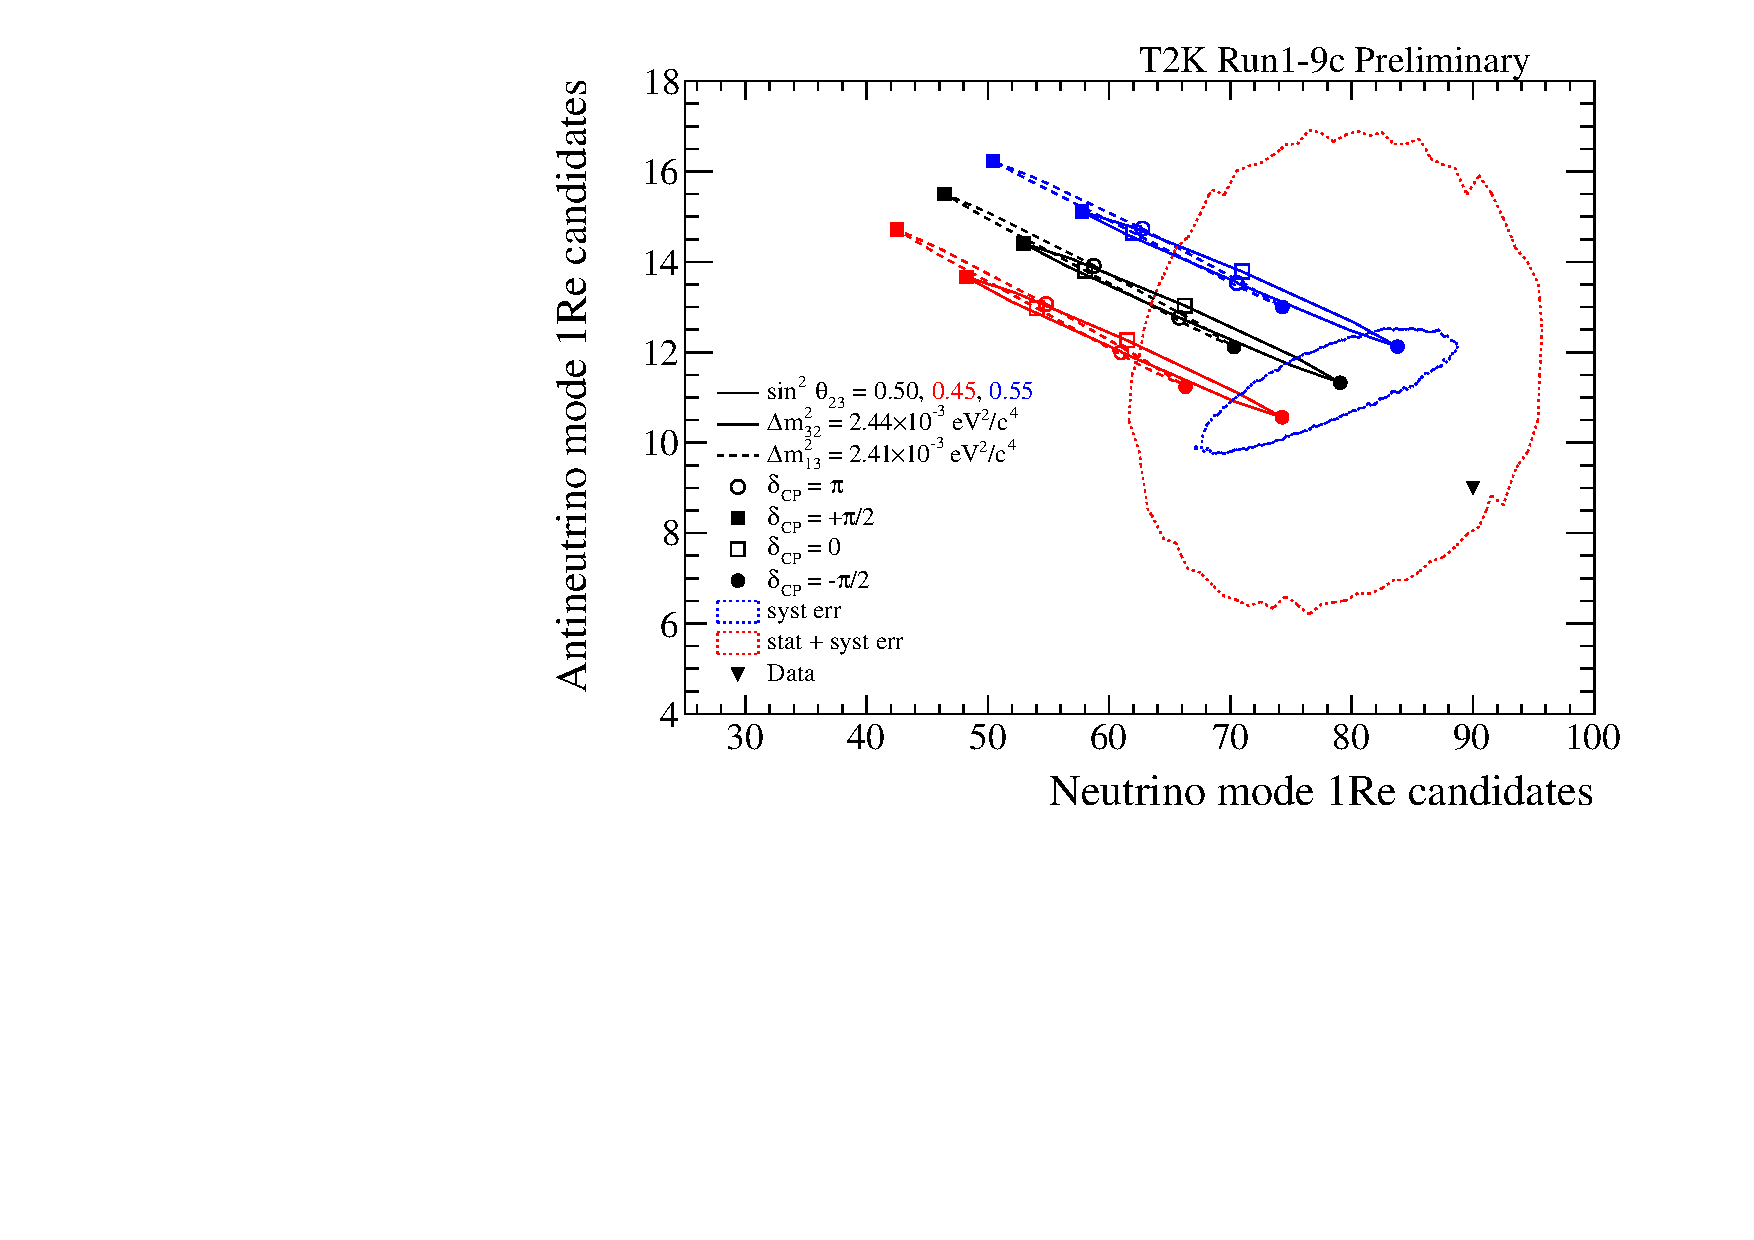
\includegraphics[width=0.7\textwidth]{images/bievent/bievent}
	\caption {
		This plot shows the candidate RHC one-ring $e$-like event rate vs the candidate FHC one-ring $e$-like event rate for a variety of different oscillation parameter values. Predictions are generated for best-fit values of oscillation parameters for different values of \deltacp, \ssqthtwothree and mass hierarchy.
	}
	\label{fig:bievent}
\end{figure*}

\clearpage

%%% Local Variables:
%%% mode: latex
%%% TeX-master: "../TN327"
%%% End:

\clearpage
\section{Comparison of \RunPeriod{} results to \PrevRunPeriod{}}
\label{sec:comparison}

This chapter compares the results for the current \RunPeriod data set to the results obtained for the previous \PrevRunPeriod data set. Comparisons of \RunPeriod data to Asimov A sensitivities can be found in \cref{app:data_asimov_comparison}, whilst comparisons between sensitivity studies from the respective periods can be found in \cref{app:asimov_comparison}. Comparisons of data fits and sensitivity studies between the different fitting groups can be found in \cref{app:group_comparison}.

\subsection{Results for \appearance}
In \cref{fig:ssqth13_vs_dcp_data_compare} the result for \appearance with reactor constraint and T2K only is shown. The additional data gathered since \PrevRunPeriod has resulted in a small decrease in the contour in the \deltacp dimension with the reactor constraint applied, with a more substantial decrease evident in the case where the reactor constraint is not applied.

\begin{figure*}[htb]
	\center
	\begin{subfigure}[b]{0.49\textwidth}
		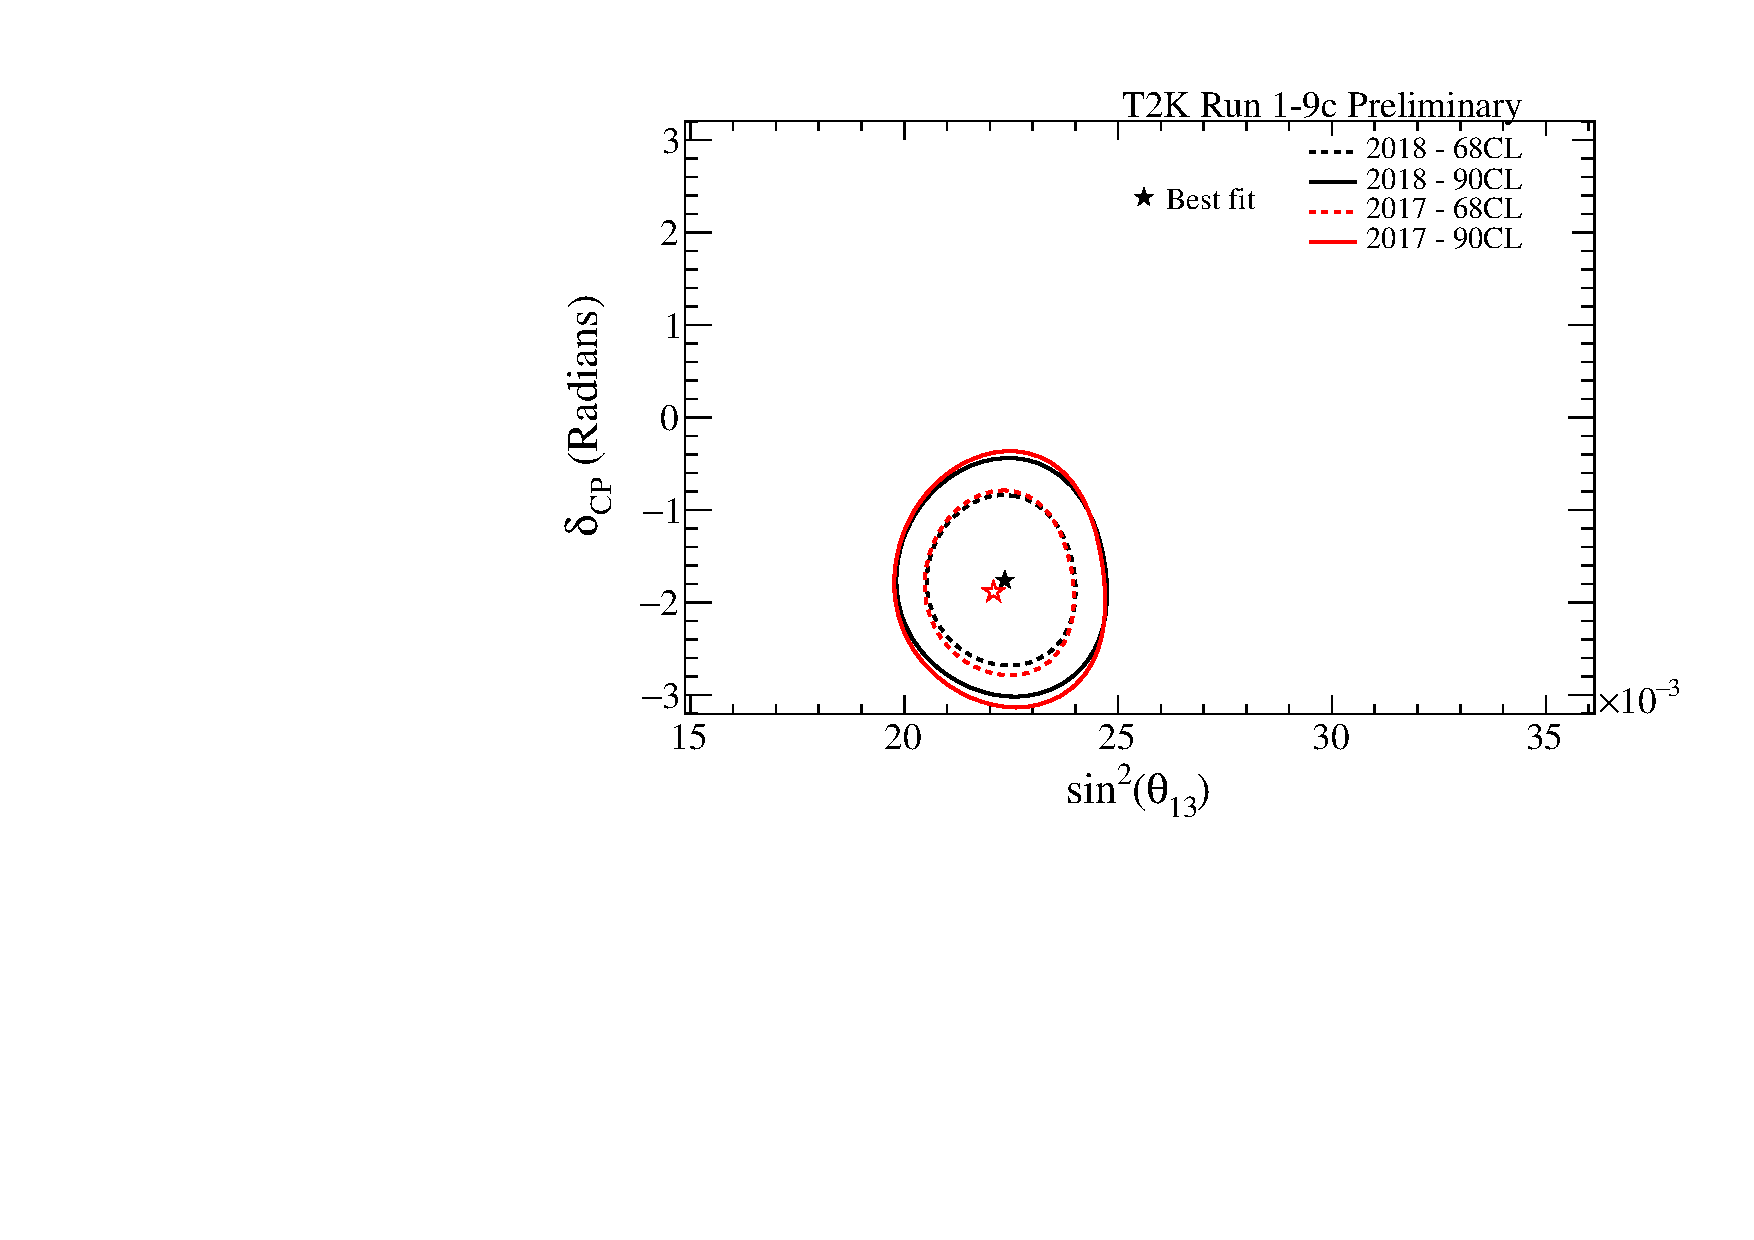
\includegraphics[width=0.9\textwidth]{images/data/comparison/appearance_wrc_normal_2018_v_2017}
		\caption{\appearance NH with reactor constraint}
	\end{subfigure}
	\begin{subfigure}[b]{0.49\textwidth}
		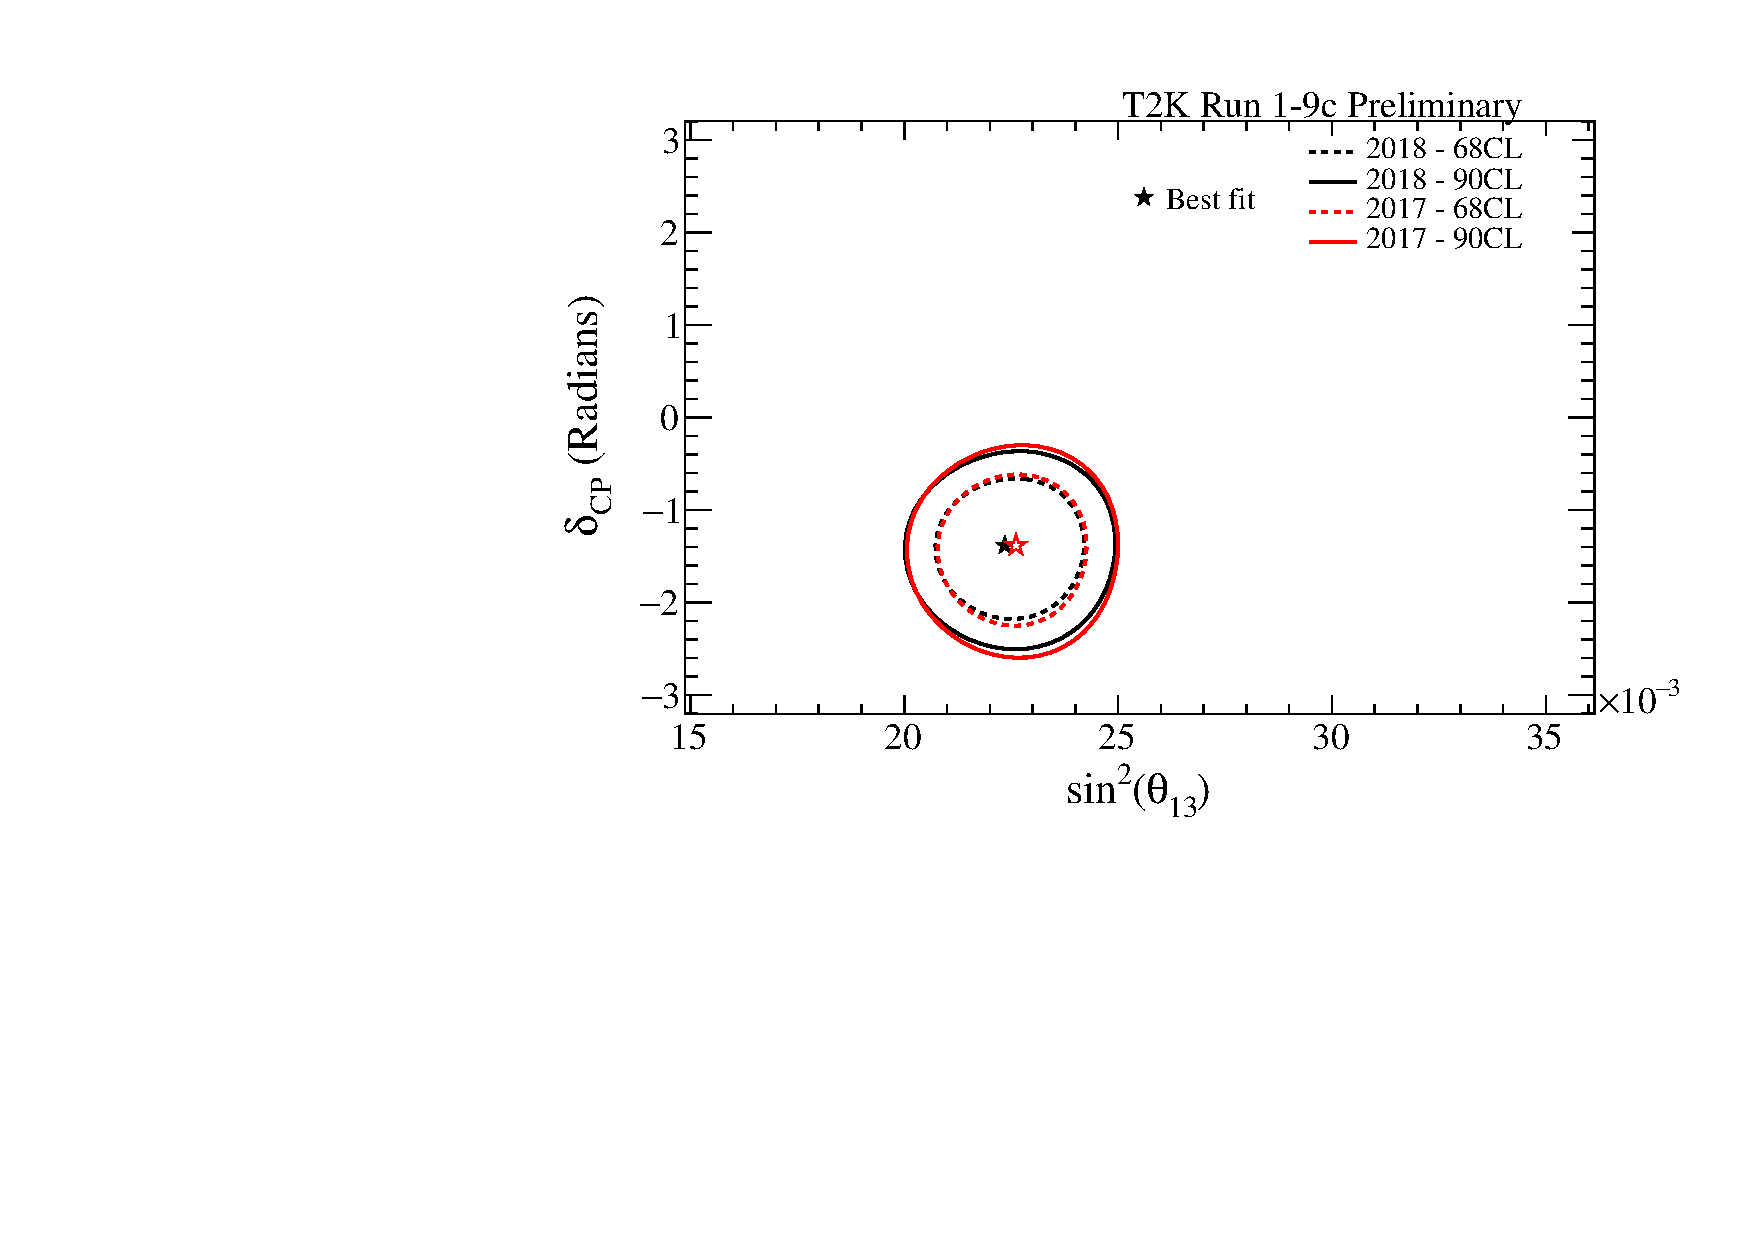
\includegraphics[width=0.9\textwidth]{images/data/comparison/appearance_wrc_inverted_2018_v_2017}
		\caption{\appearance IH with reactor constraint}
	\end{subfigure}
	\begin{subfigure}[b]{0.49\textwidth}
		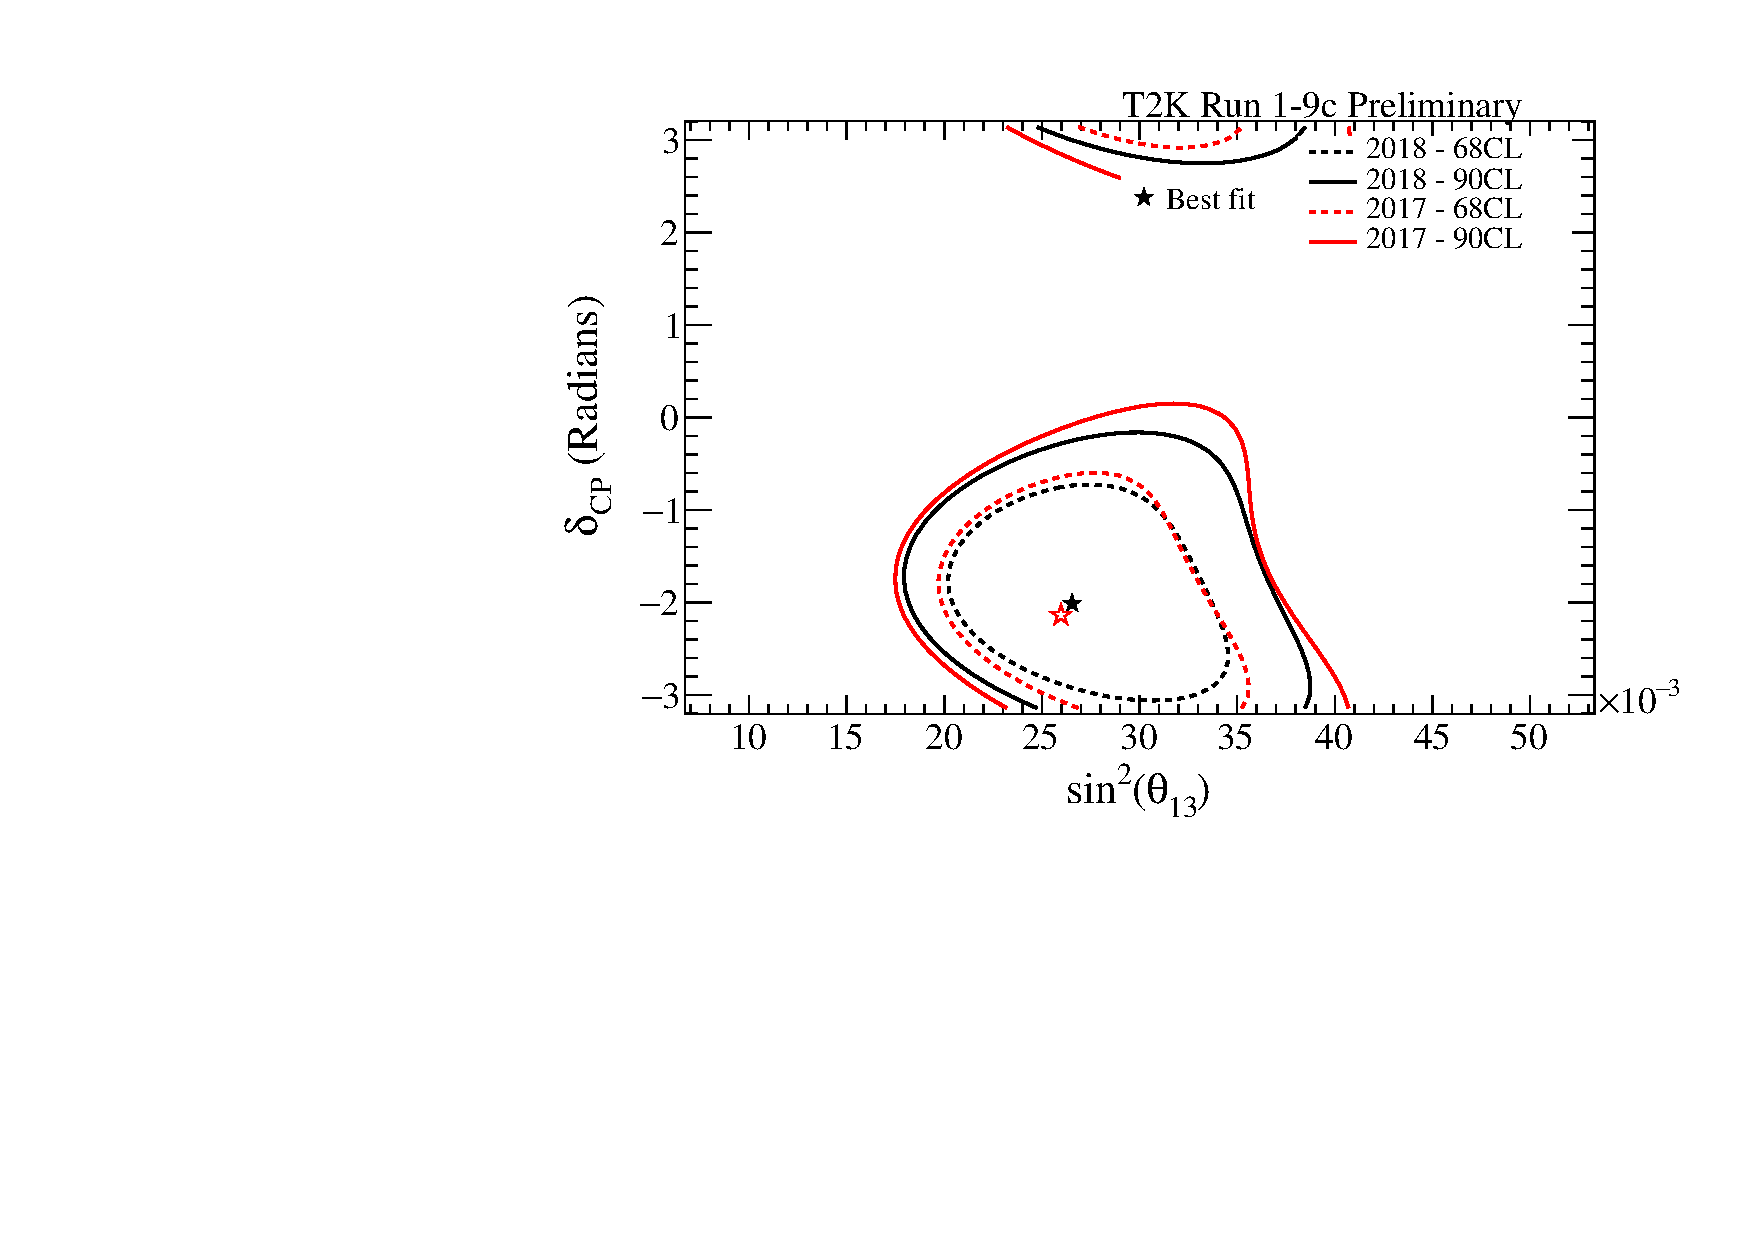
\includegraphics[width=0.9\textwidth]{images/data/comparison/appearance_worc_normal_2018_v_2017}
		\caption{\appearance NH without reactor constraint}
	\end{subfigure}
	\begin{subfigure}[b]{0.49\textwidth}
		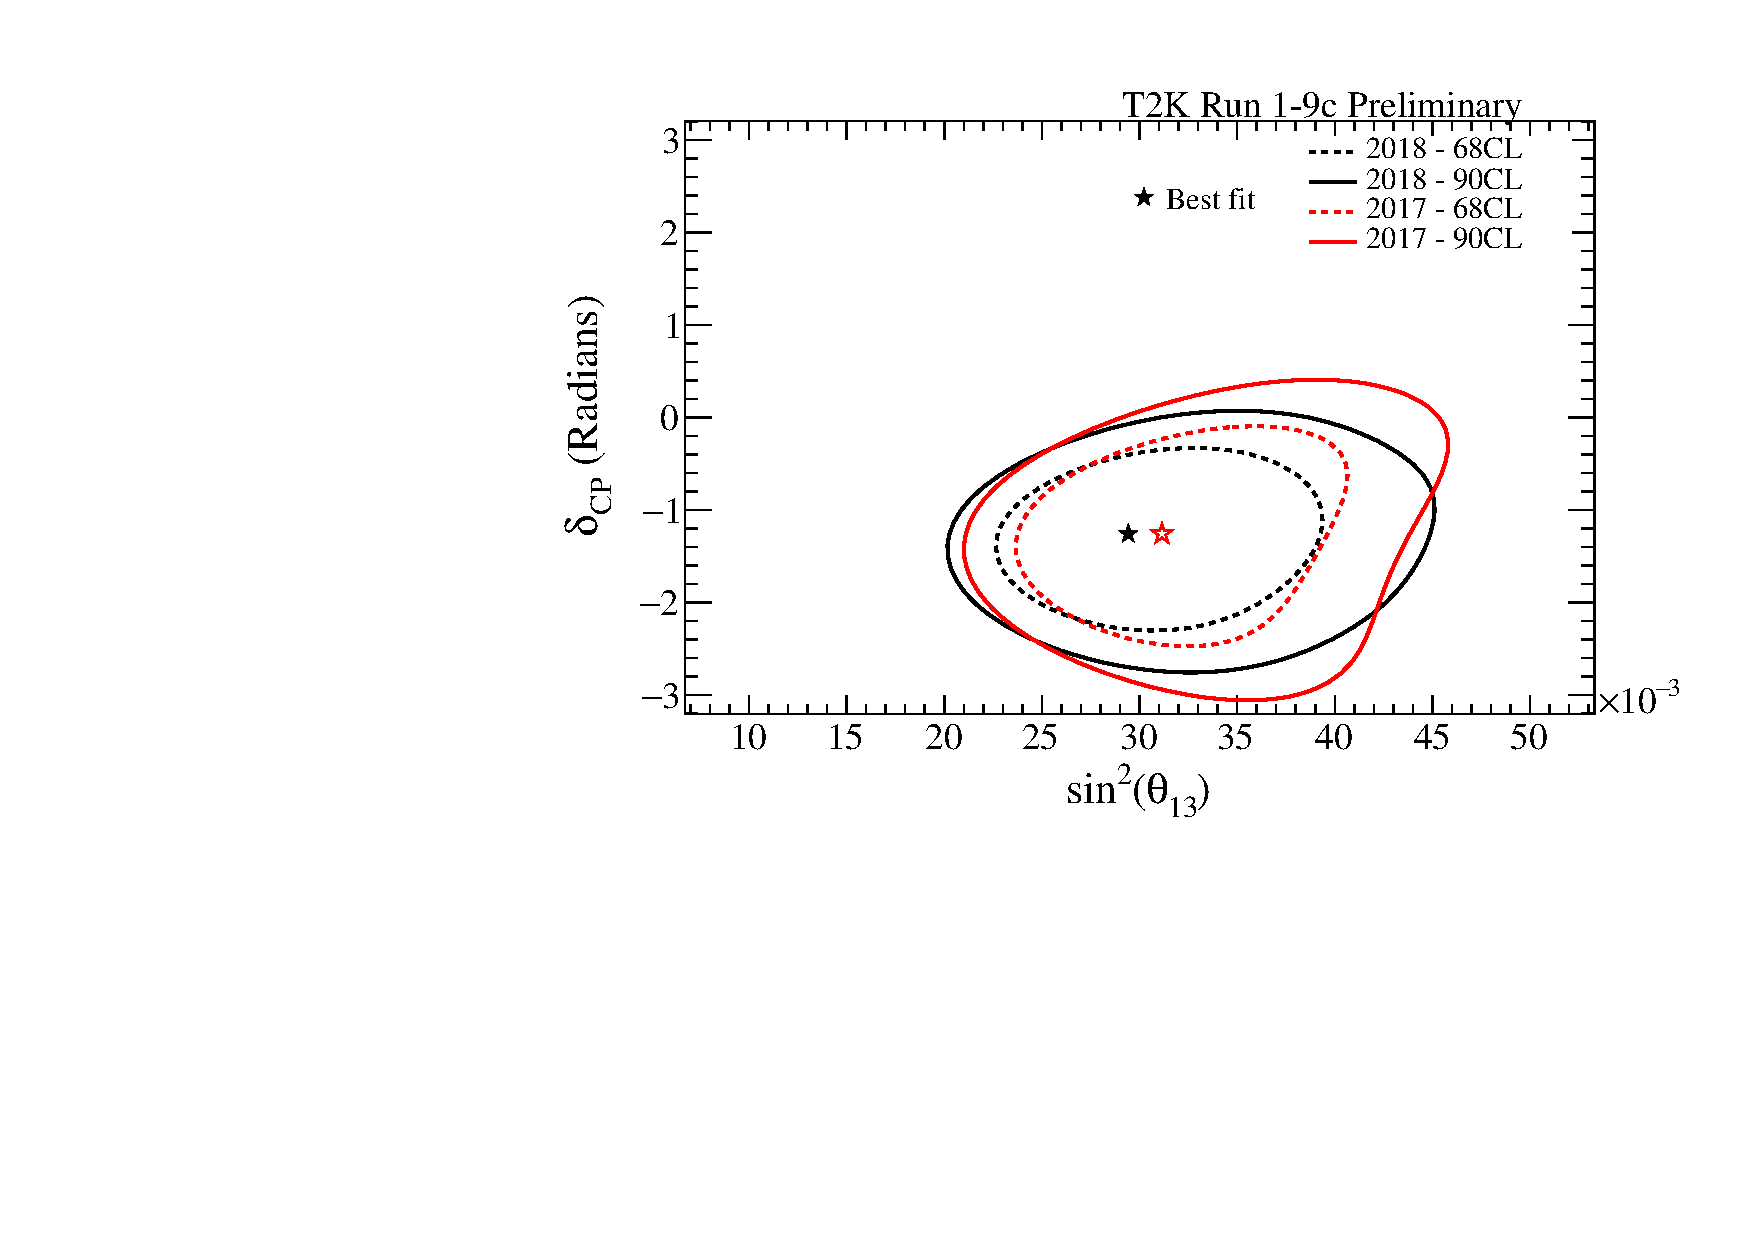
\includegraphics[width=0.9\textwidth]{images/data/comparison/appearance_worc_inverted_2018_v_2017}
		\caption{\appearance IH without reactor constraint}
	\end{subfigure}
	\caption {
		Contours at 68\% and 90\% CL for \appearance with and without reactor constraint. Normal and inverted hierarchy contours are independent. All 5 samples were used to produce these fits.
	}
	\label{fig:ssqth13_vs_dcp_data_compare}
\end{figure*}
\clearpage

\subsection{Results for \disappearance}

The result for \disappearance with reactor constraint and T2K only is shown in fig.~\ref{fig:ssqth23_vs_dmsq_data_compare}. The notable changes in the disappearance fits are a shift of the contour towards lower values of \dmsq (for both normal and inverted hierarchy), a move away from maximal disappearance and a broadening of the contour in the \ssqthtwothree dimension.

\begin{figure*}[htb]
	\center
	\begin{subfigure}[b]{0.49\textwidth}
		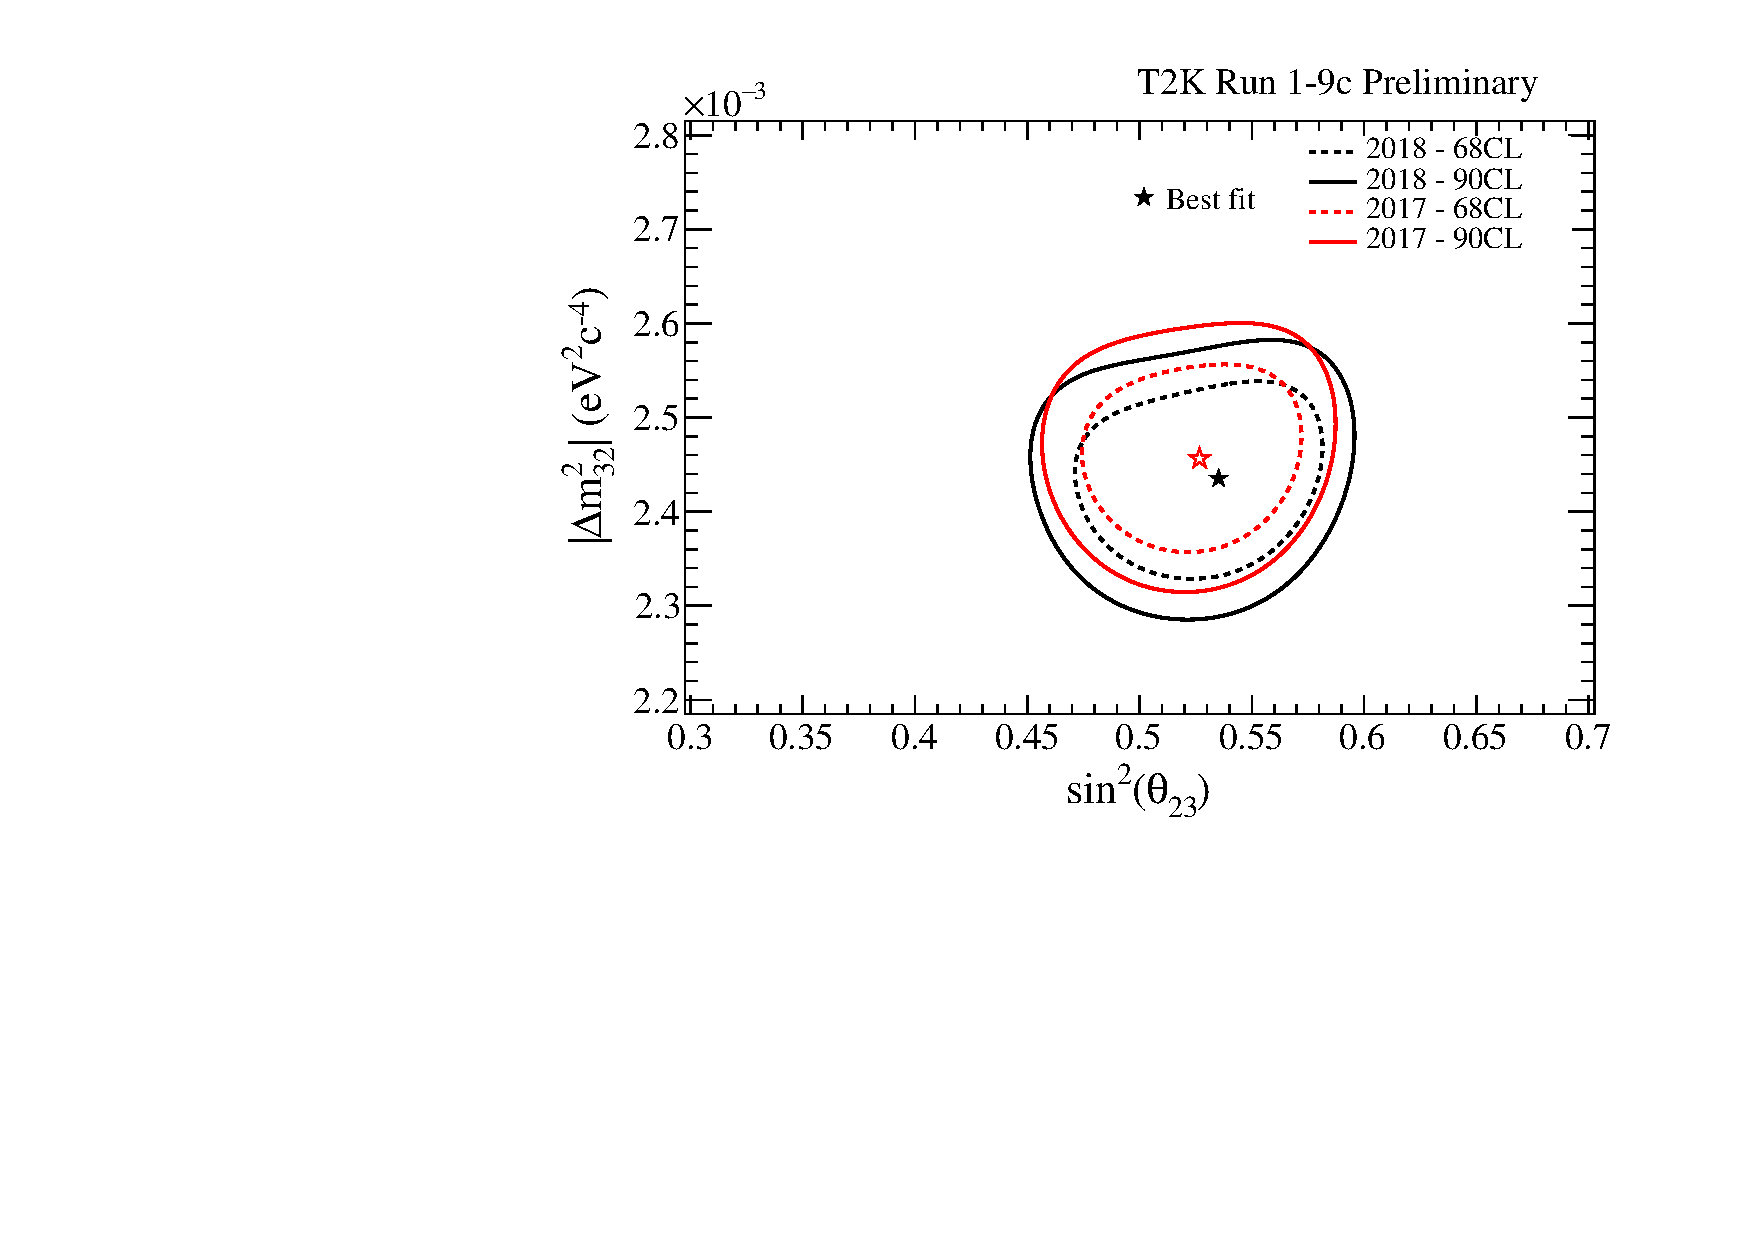
\includegraphics[width=0.9\textwidth]{images/data/comparison/disappearance_wrc_normal_2018_v_2017}
		\caption{\disappearance NH with reactor constraint}
	\end{subfigure}
	\begin{subfigure}[b]{0.49\textwidth}
		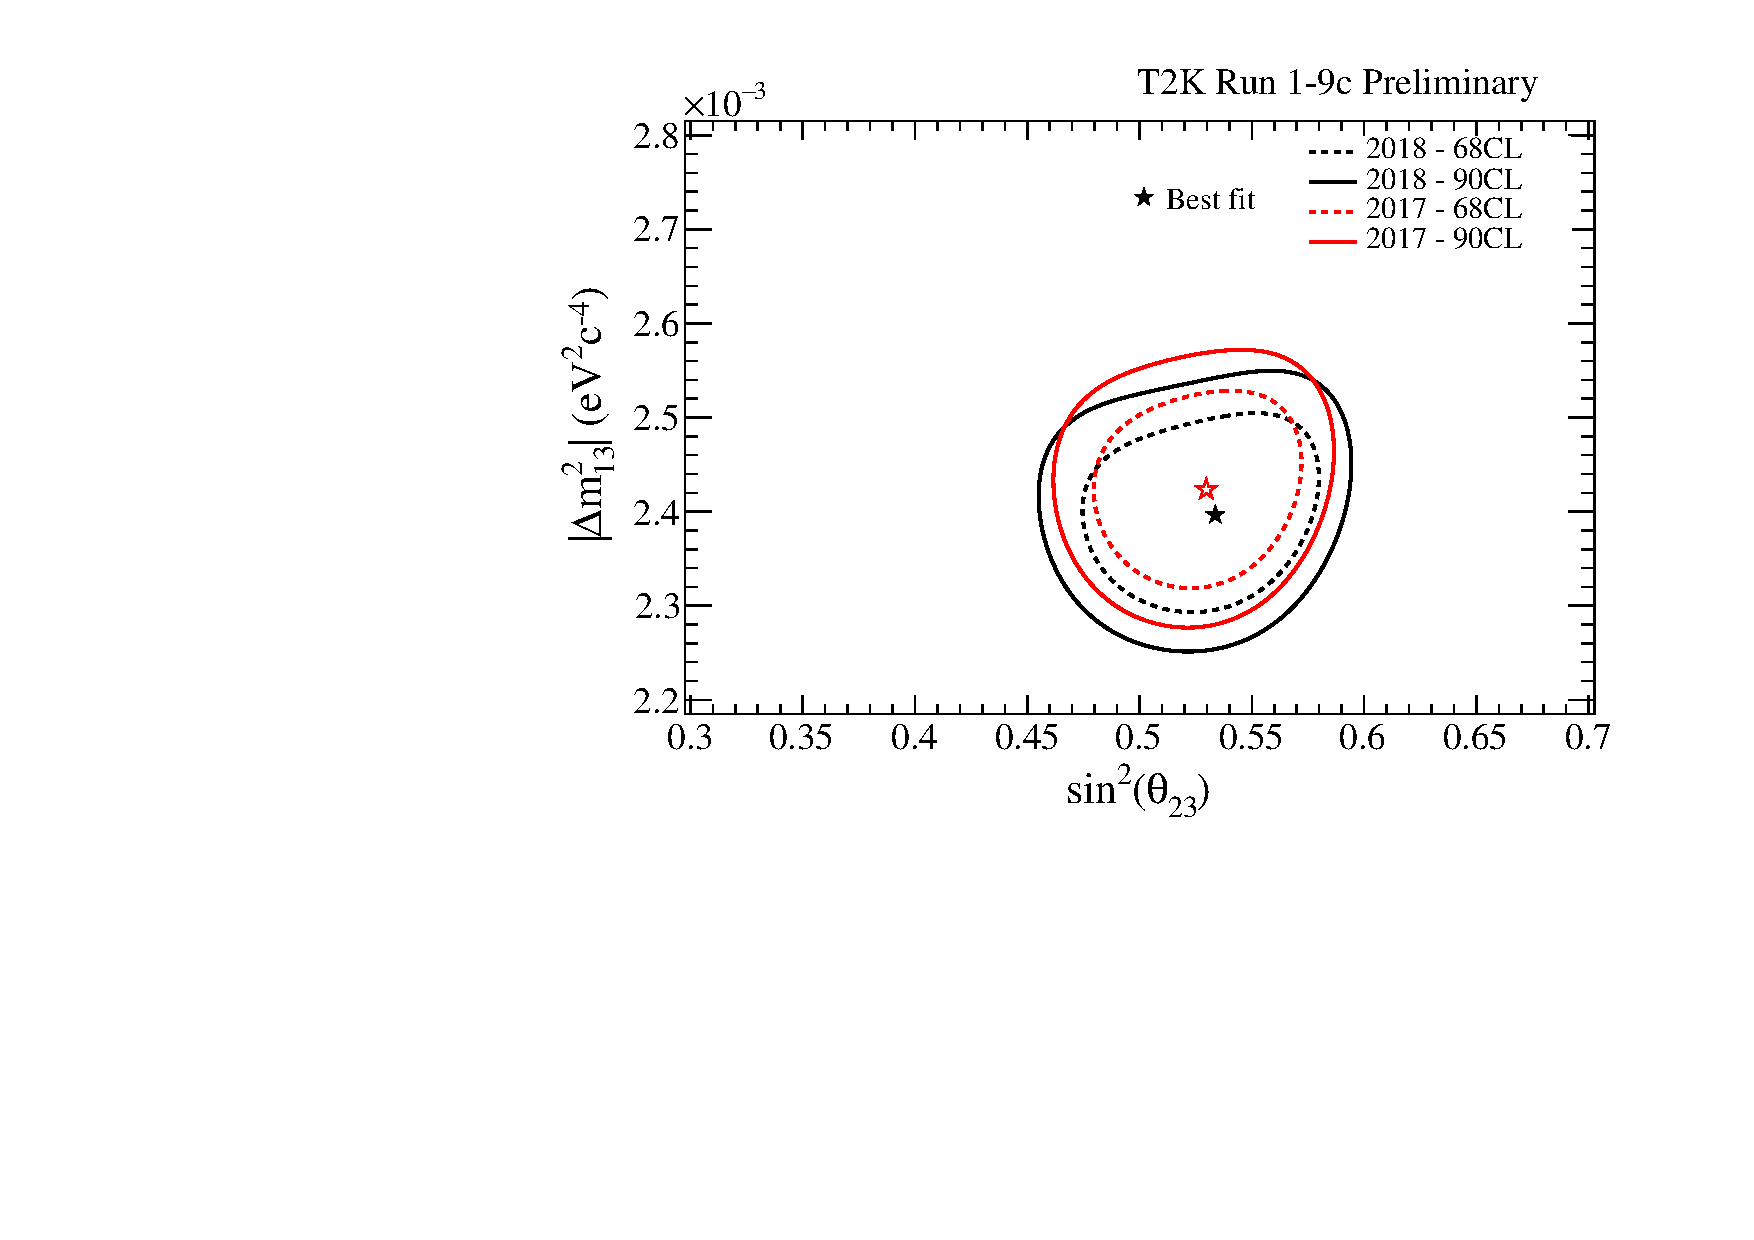
\includegraphics[width=0.9\textwidth]{images/data/comparison/disappearance_wrc_inverted_2018_v_2017}
		\caption{\disappearance IH with reactor constraint}
	\end{subfigure}
	\begin{subfigure}[b]{0.49\textwidth}
		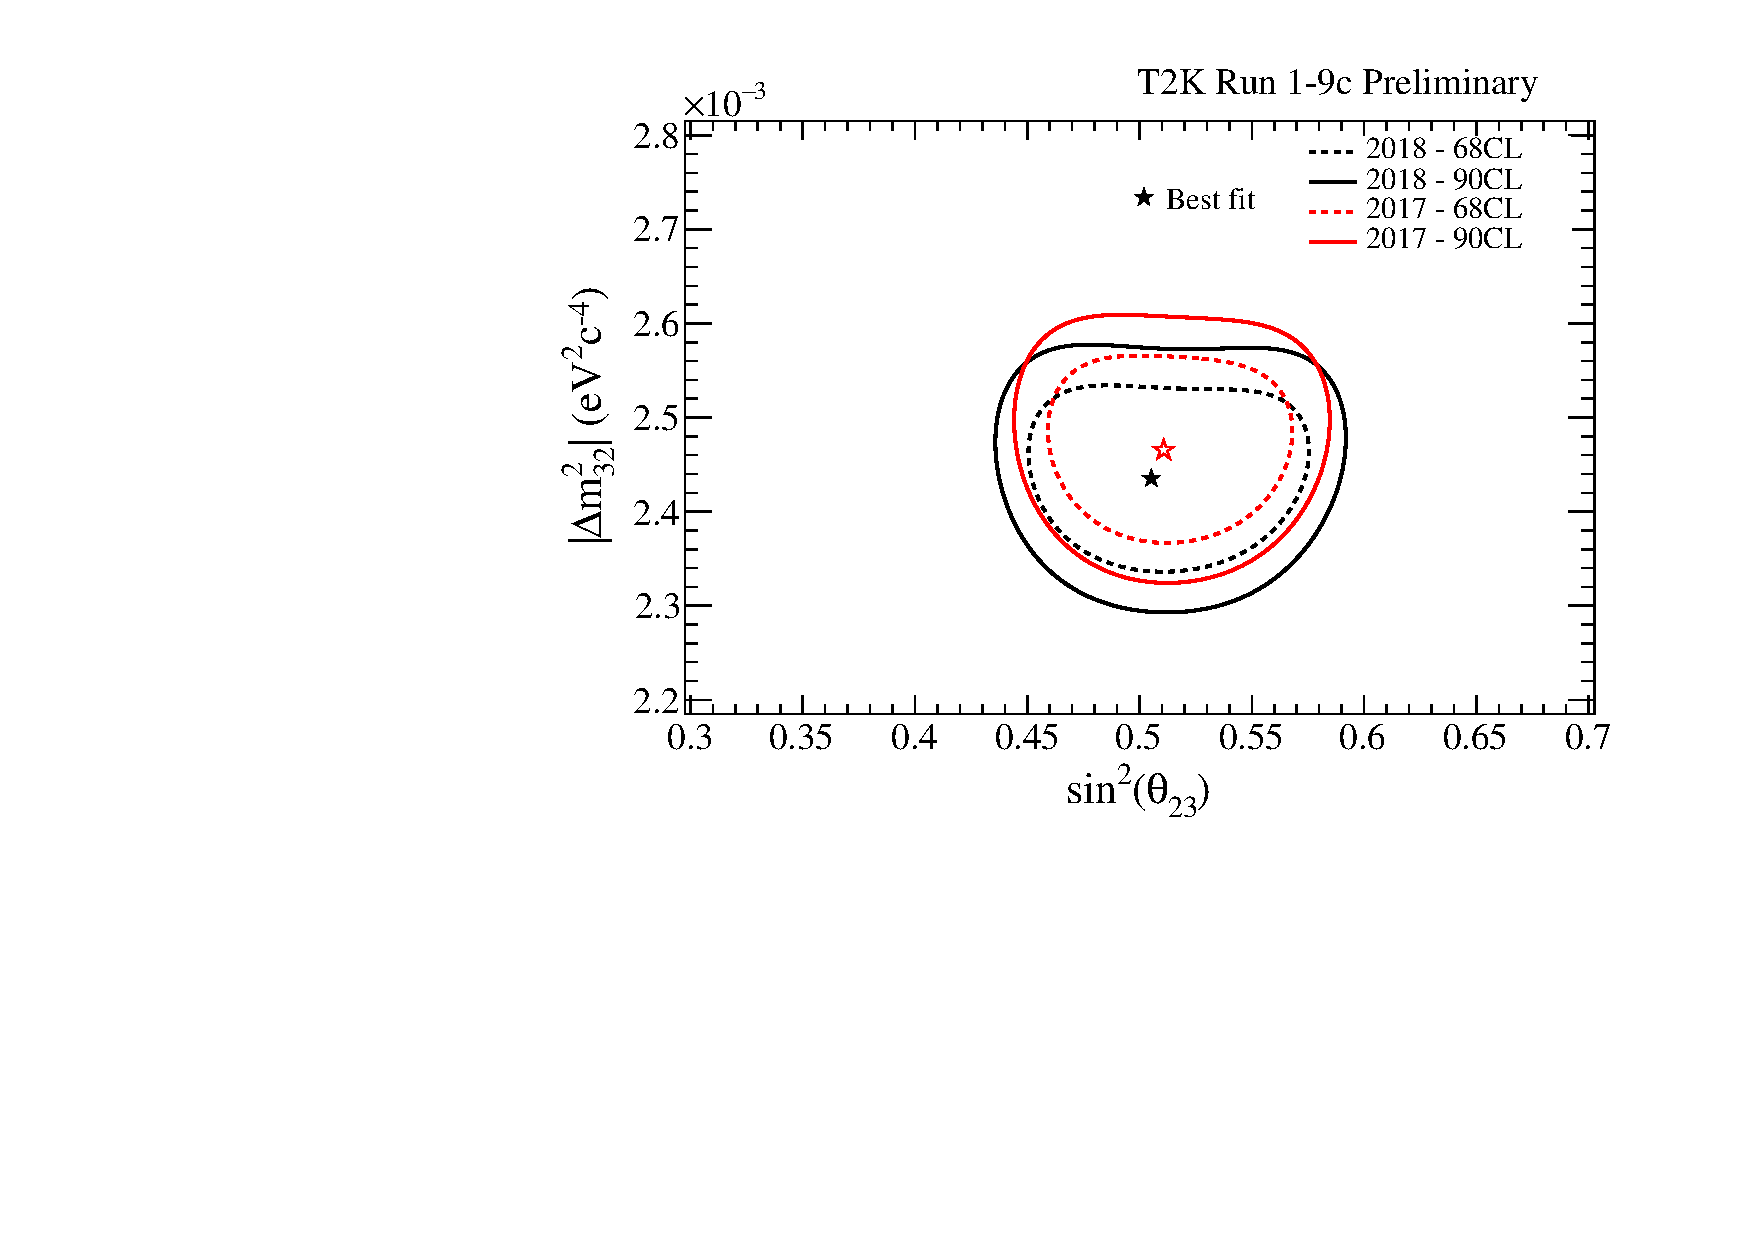
\includegraphics[width=0.9\textwidth]{images/data/comparison/disappearance_worc_normal_2018_v_2017}
		\caption{\disappearance NH without reactor constraint}
	\end{subfigure}
	\begin{subfigure}[b]{0.49\textwidth}
		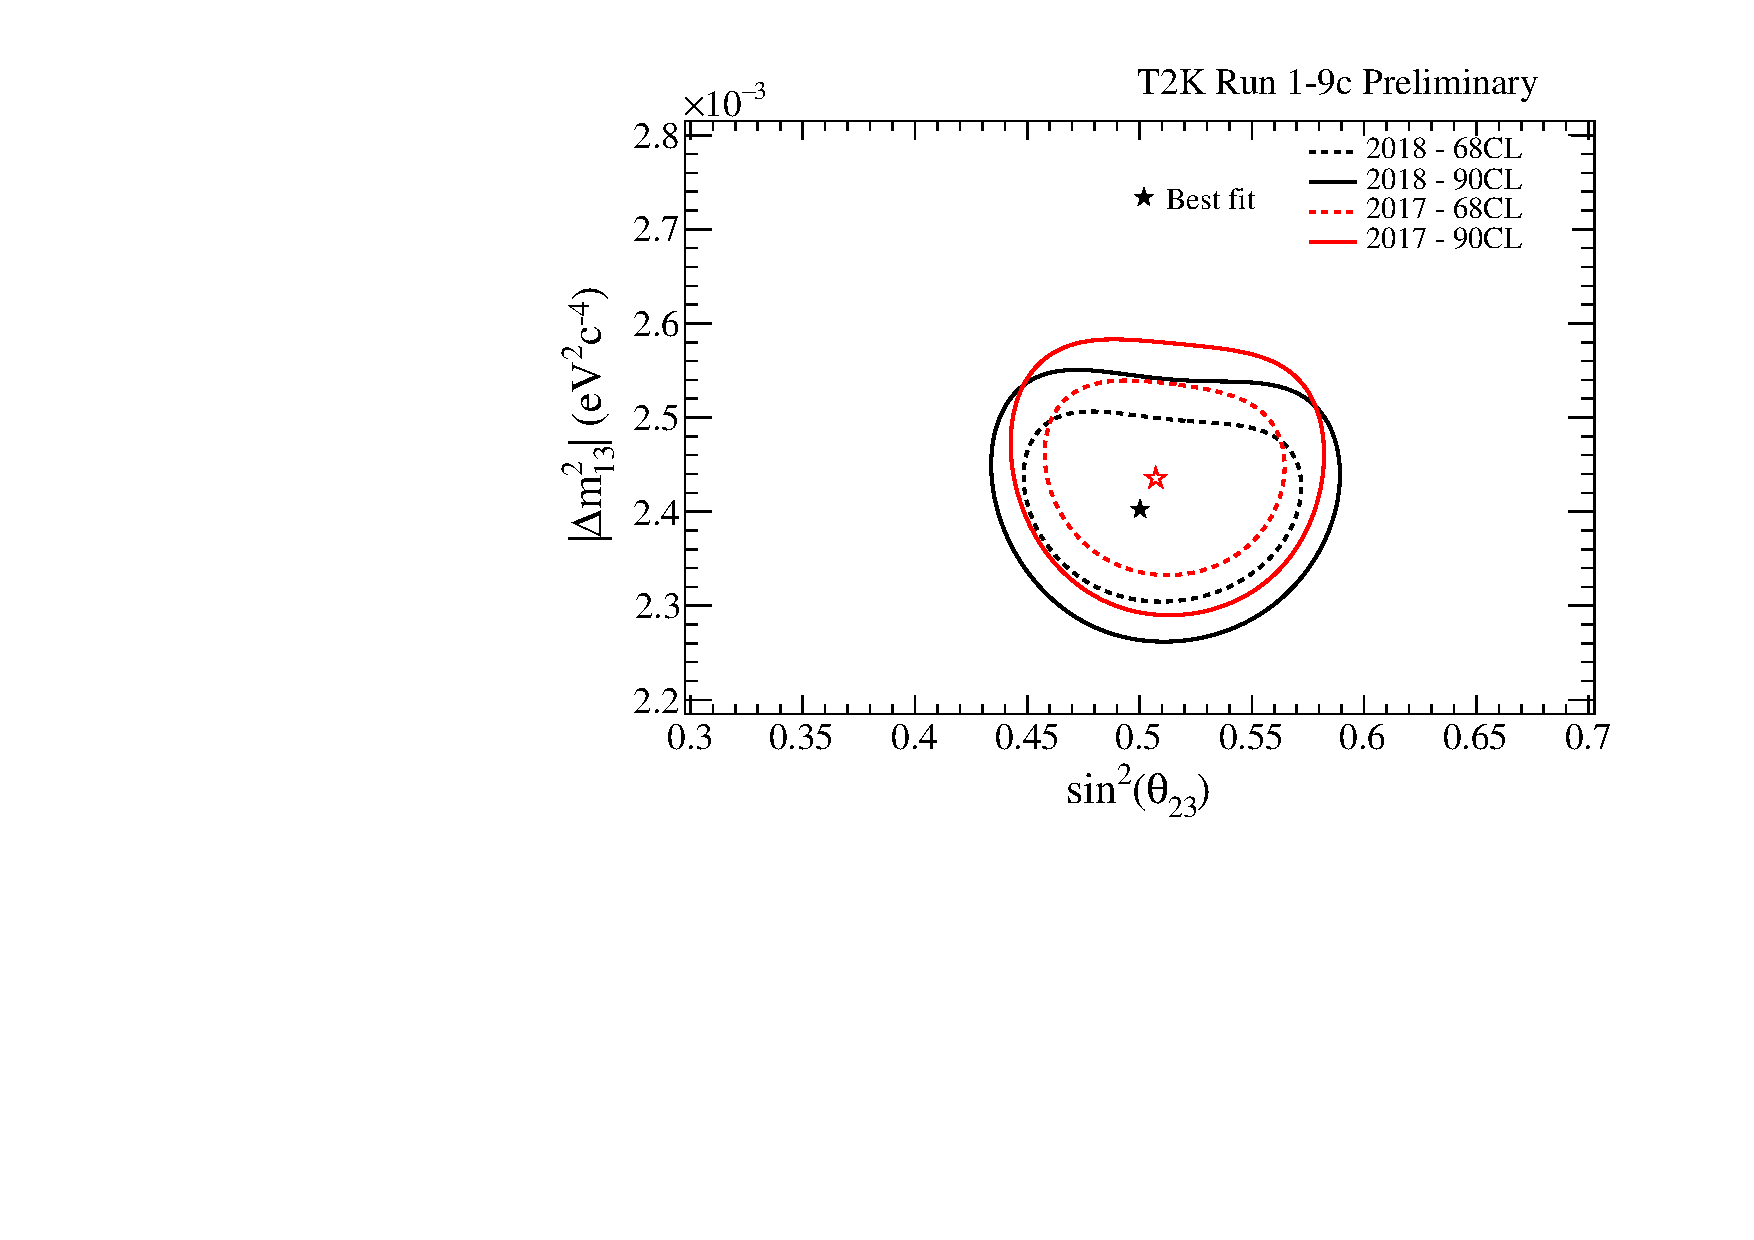
\includegraphics[width=0.9\textwidth]{images/data/comparison/disappearance_worc_inverted_2018_v_2017}
		\caption{\disappearance IH without reactor constraint}
	\end{subfigure}
	\caption {
		Contours at 68\% and 90\% CL for \disappearance with and without reactor constraint. Normal and inverted hierarchy contours are independent. All 5 samples were used to produce these fits.
	}
	\label{fig:ssqth23_vs_dmsq_data_compare}
\end{figure*}

In \PrevRunPeriod, the data contour is both narrower and shifted with respect to the prediction of the best-fit Asimov (\cref{fig:disappearance_check}), whereas the \RunPeriod data contour shows better agreement with the best-fit prediction, though remaining somewhat narrower. The corresponding RHC one-ring $\mu$-like observed and best-fit spectra are also shown. Therefore, the broadening of the contour in \RunPeriod can be explained as the result of a shift towards a more PMNS-like result.

\begin{figure*}[htb]
	\center
	\begin{subfigure}[b]{0.49\textwidth}
		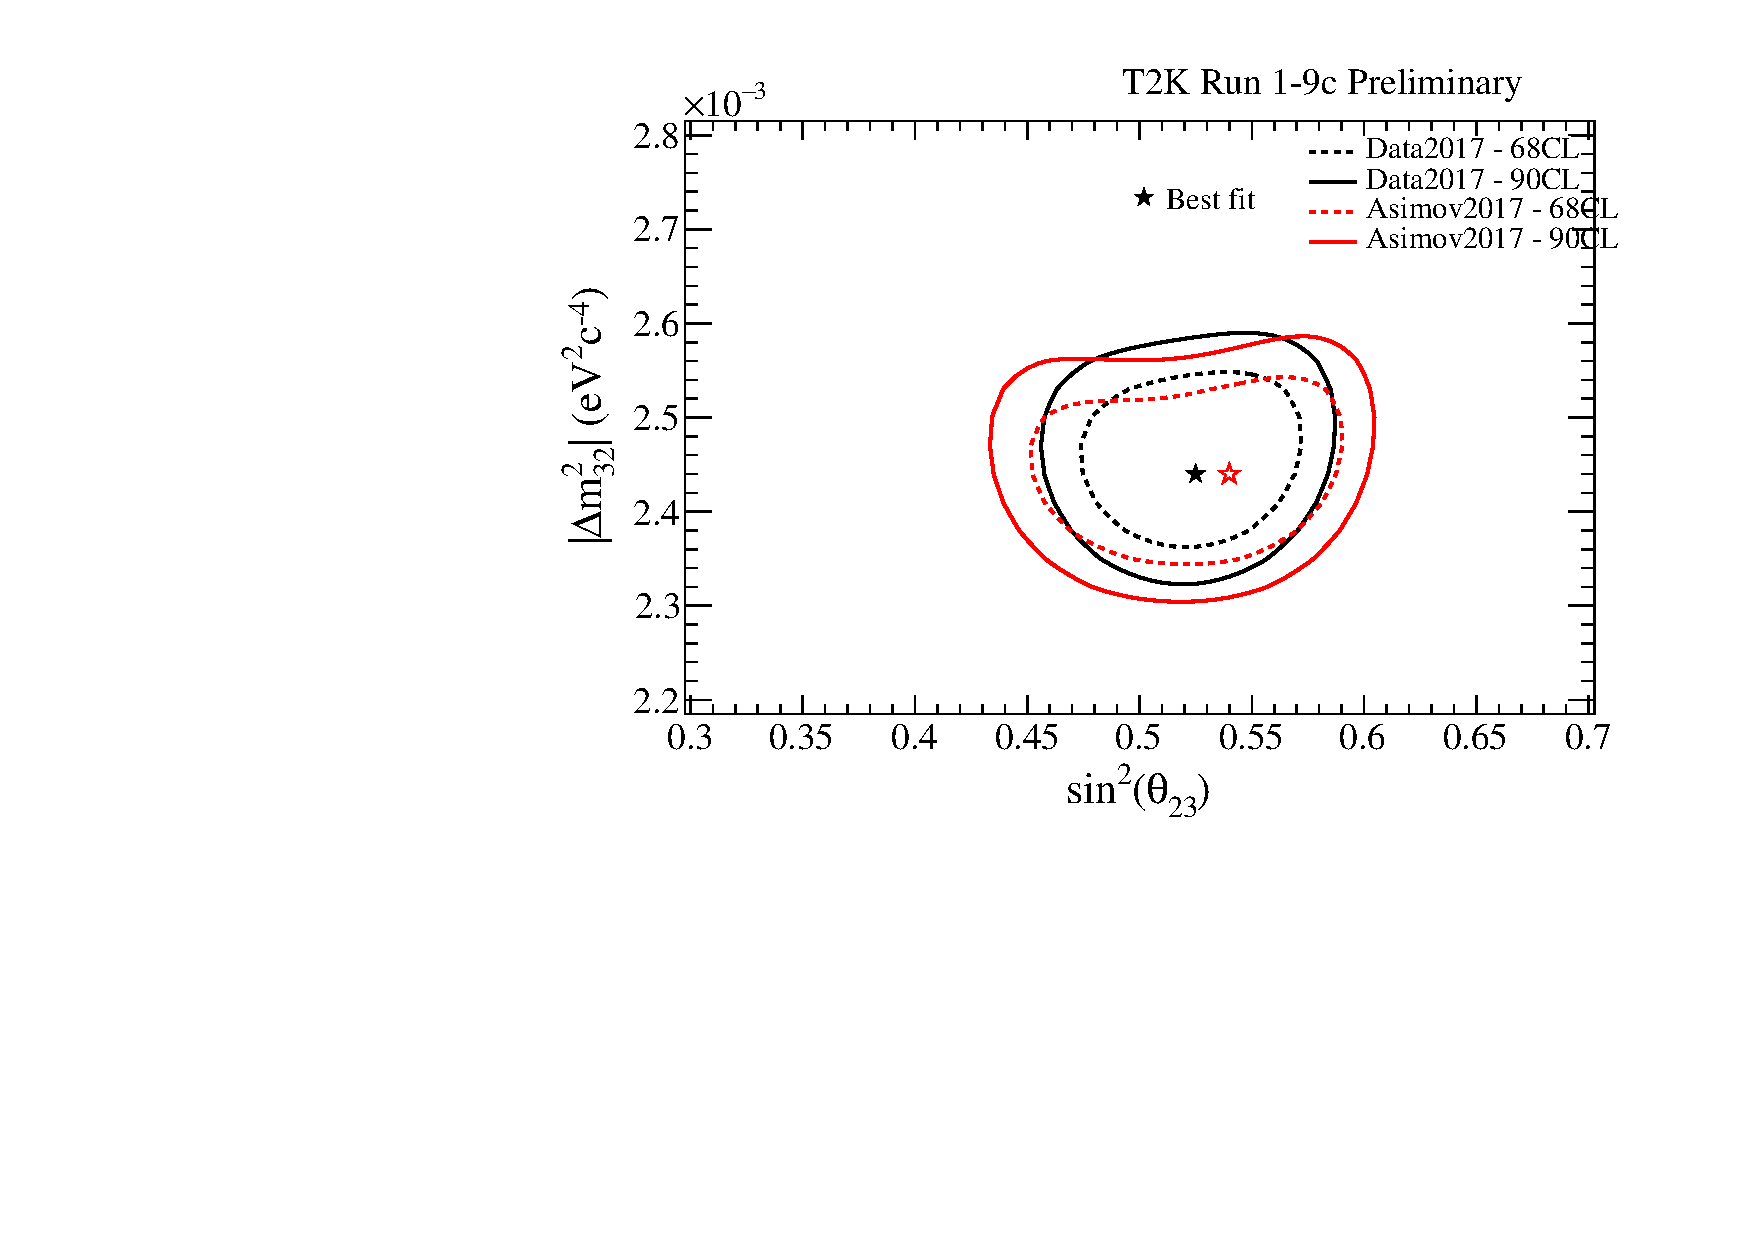
\includegraphics[width=0.9\textwidth]{images/checks/disappearance/Data2017_v_Asimov2017}
		\caption{\PrevRunPeriod}
	\end{subfigure}
	\begin{subfigure}[b]{0.49\textwidth}
		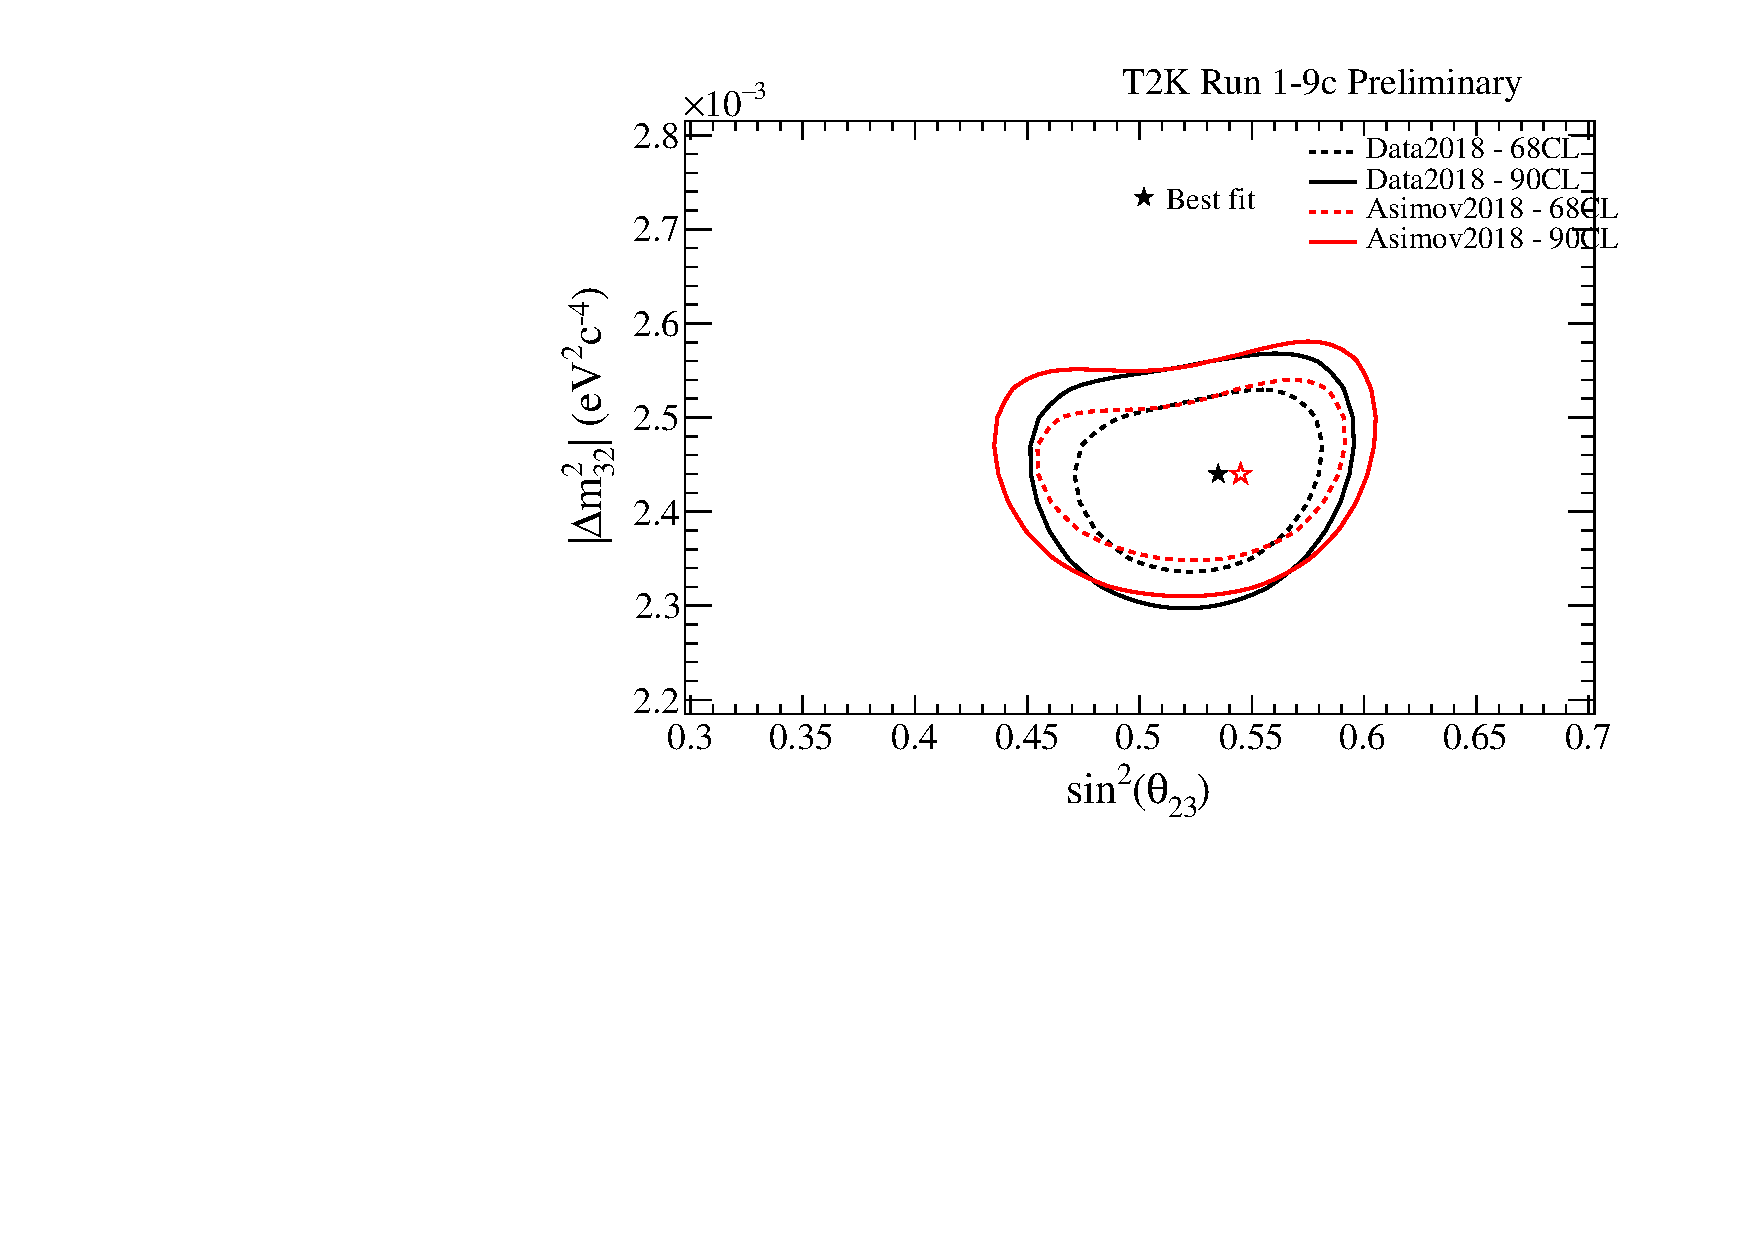
\includegraphics[width=0.9\textwidth]{images/checks/disappearance/Data2018_v_Asimov2018}
		\caption{\RunPeriod}
	\end{subfigure}
	
	\begin{subfigure}[b]{0.49\textwidth}
		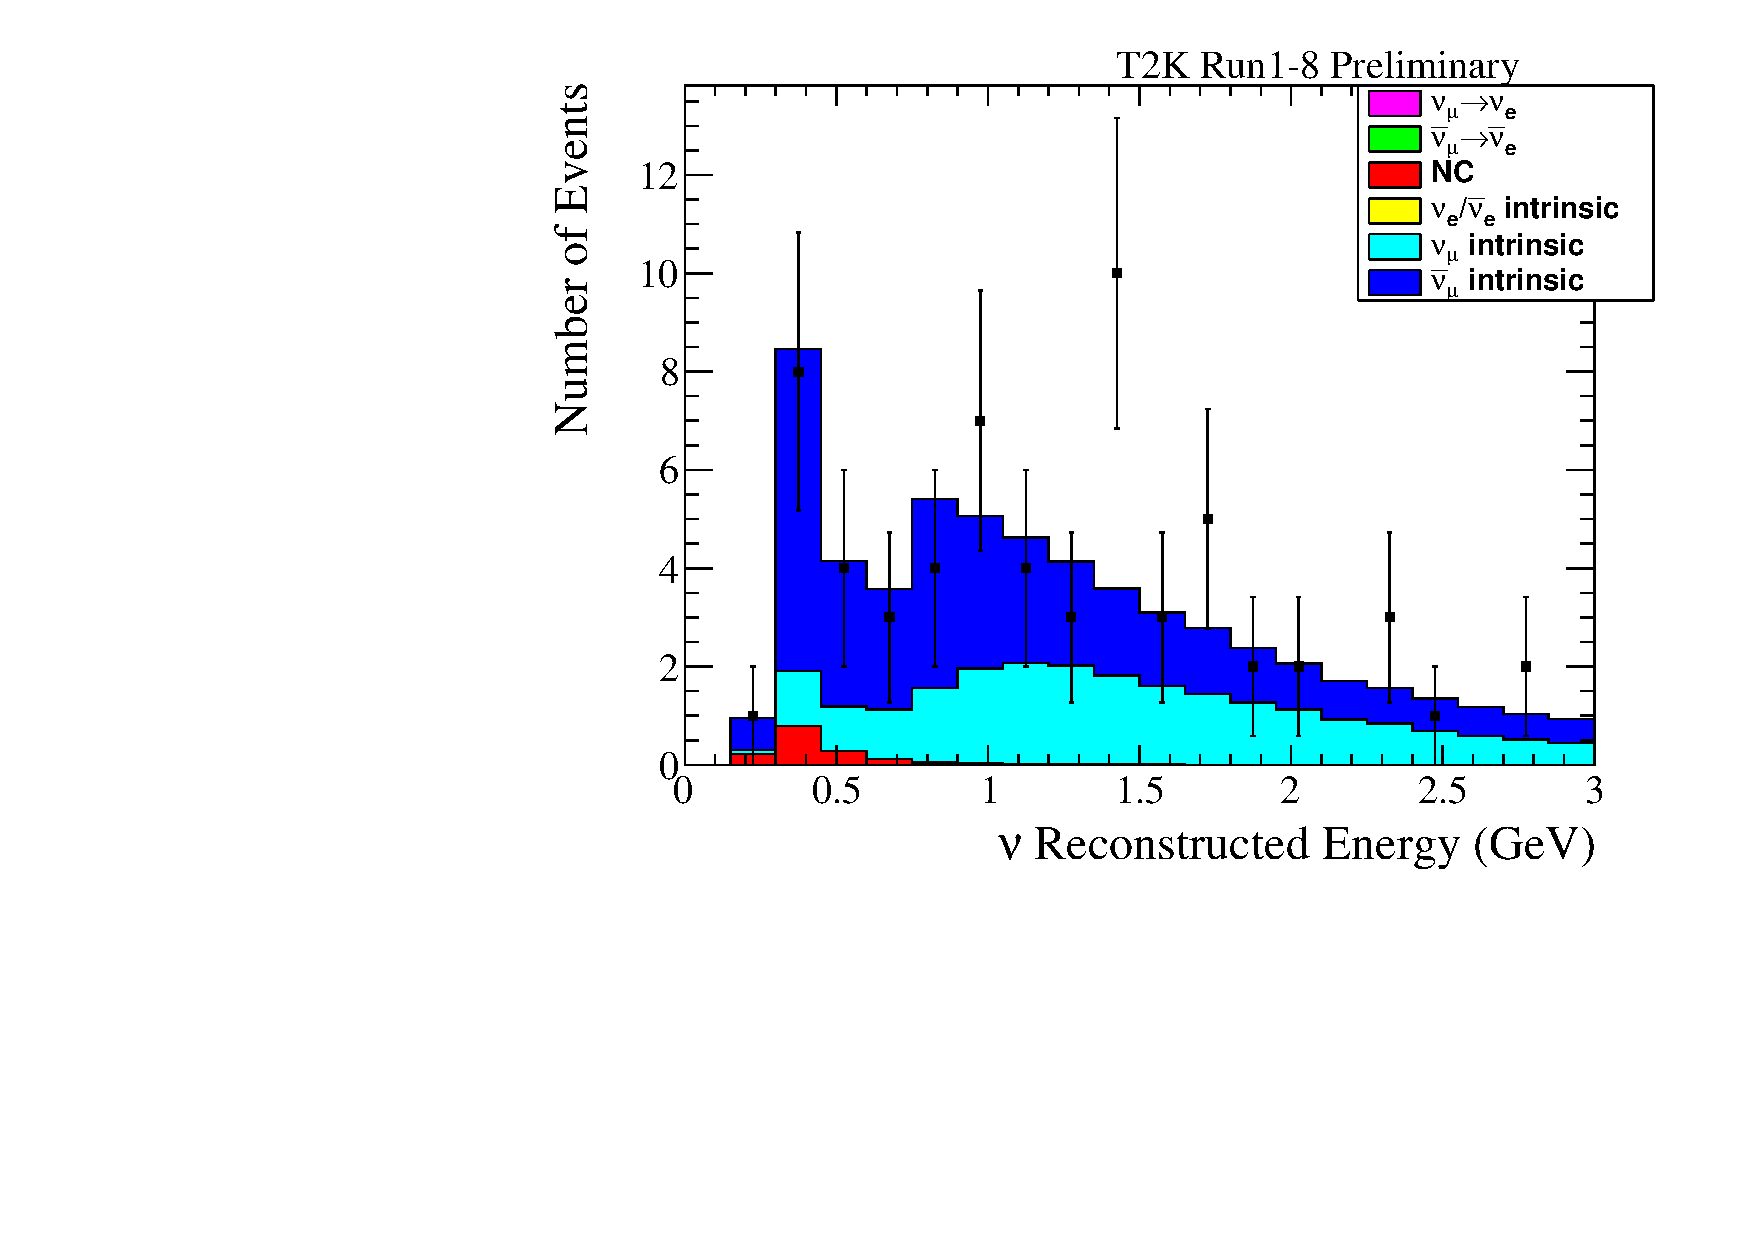
\includegraphics[width=0.9\textwidth]{images/checks/disappearance/spectrum_asimov2017_RHC1Rmu_data}
		\caption{\PrevRunPeriod RHC one-ring $\mu$-like spectra}
	\end{subfigure}
	\begin{subfigure}[b]{0.49\textwidth}
		\includegraphics[width=0.9\textwidth]{images/checks/disappearance/spectrum_asimov2018_RHC1Rmu_data}
		\caption{\RunPeriod RHC one-ring $\mu$-like spectra}
	\end{subfigure}
	\caption {
		The top row shows normal hierarchy contours at 68\% and 90\% CL for \disappearance with the reactor constraint compared to a fit of the best-fit Asimov corresponding to the stated run period. No smearing is applied. The bottom row shows the observed and predicted spectrum from \PrevRunPeriod and \RunPeriod.
	}
	\label{fig:disappearance_check}
\end{figure*}

\iffalse
A potential explanation for the broadening of the contour, despite the increase in statistics could come from a shift in the value of \ssqthtwothree away from maximal disappearance ($\sin^2\theta_{23} \simeq 0.51$).
\fi

\clearpage

\subsection{Results for \deltacp}

The result for \deltacp with reactor constraint and T2K only is shown in fig.~\ref{fig:dcp_data_compare}. The best-fit points are little changed relative to \PrevRunPeriod, though a stronger constraint is evident, particularly without the reactor constraint applied.

\begin{figure*}[htb]
	\center
	\begin{subfigure}[b]{0.49\textwidth}
		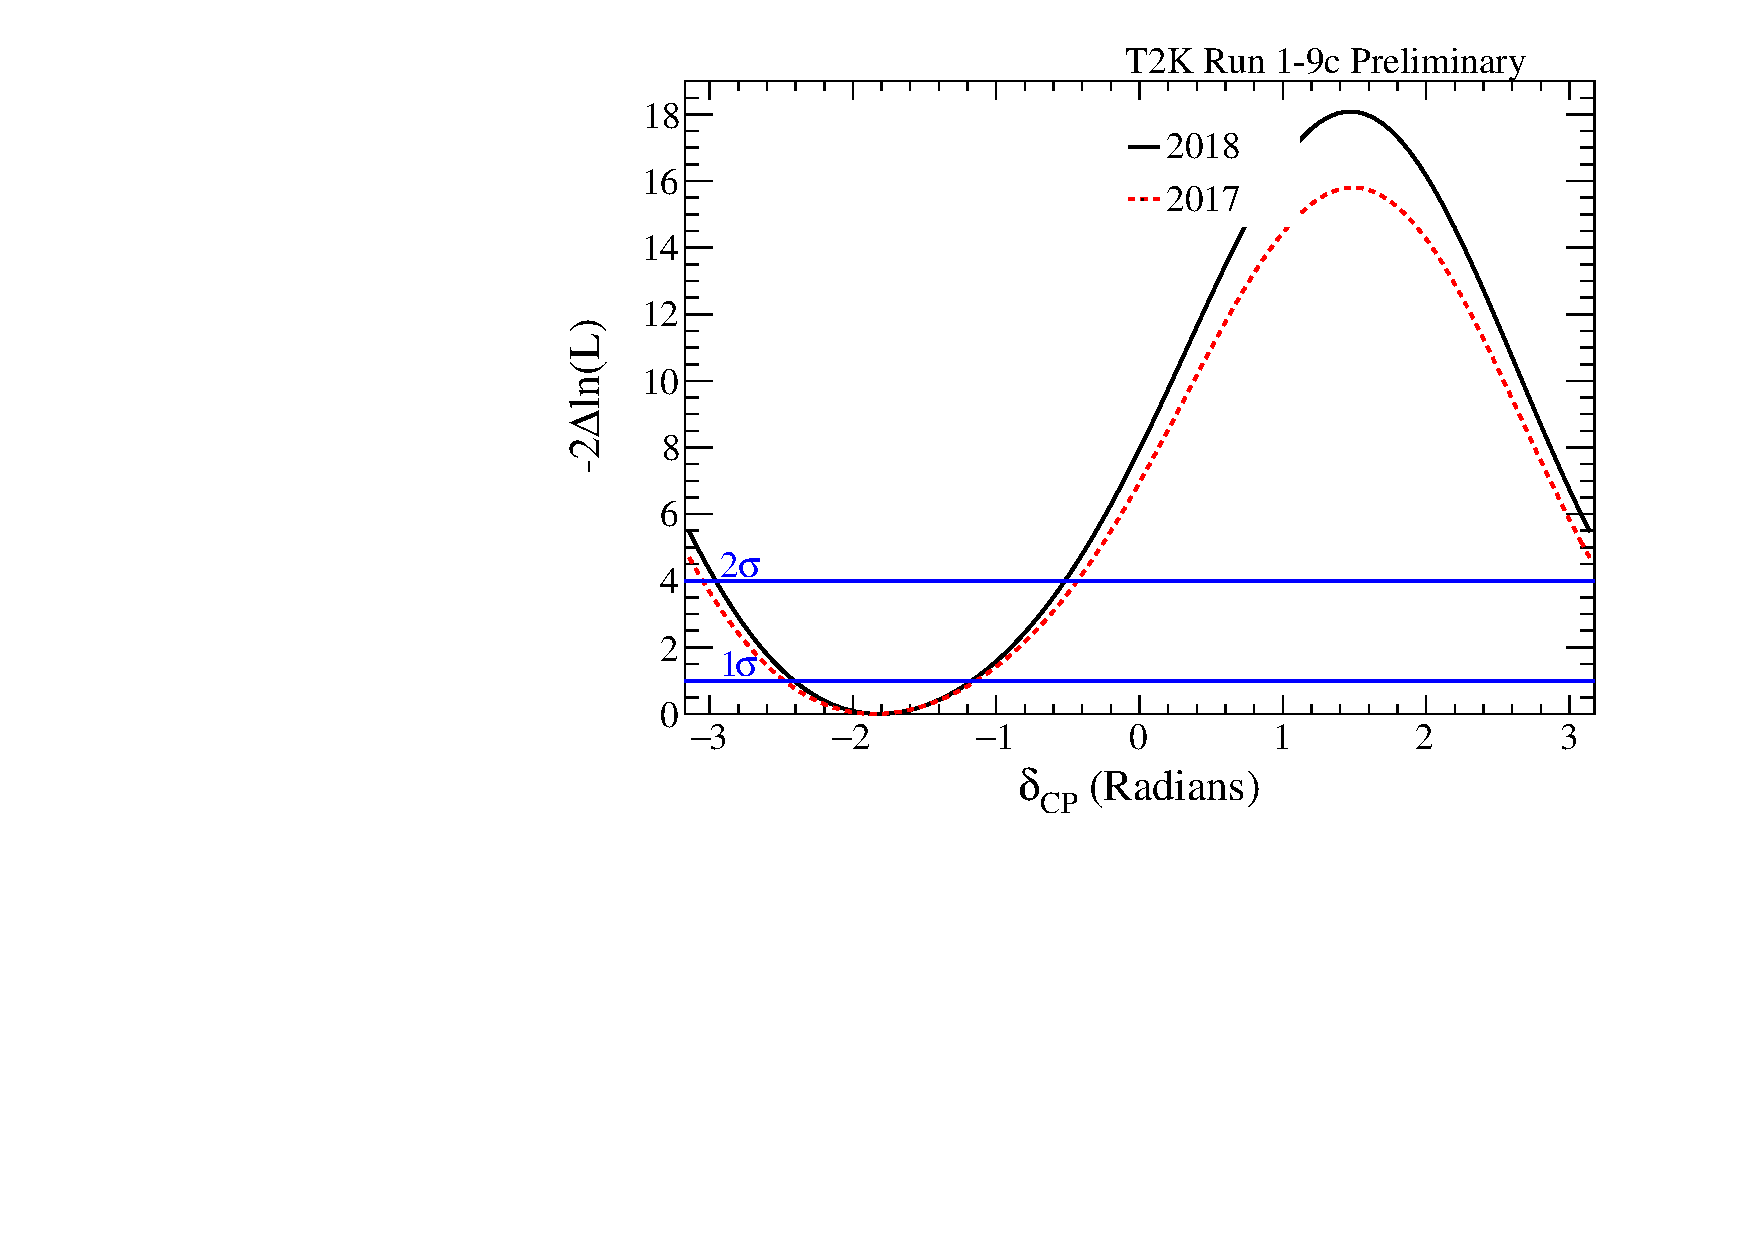
\includegraphics[width=0.9\textwidth]{images/data/comparison/deltacp_wrc_normal_2018_v_2017}
		\caption{\deltacp NH with reactor constraint}
	\end{subfigure}
	\begin{subfigure}[b]{0.49\textwidth}
		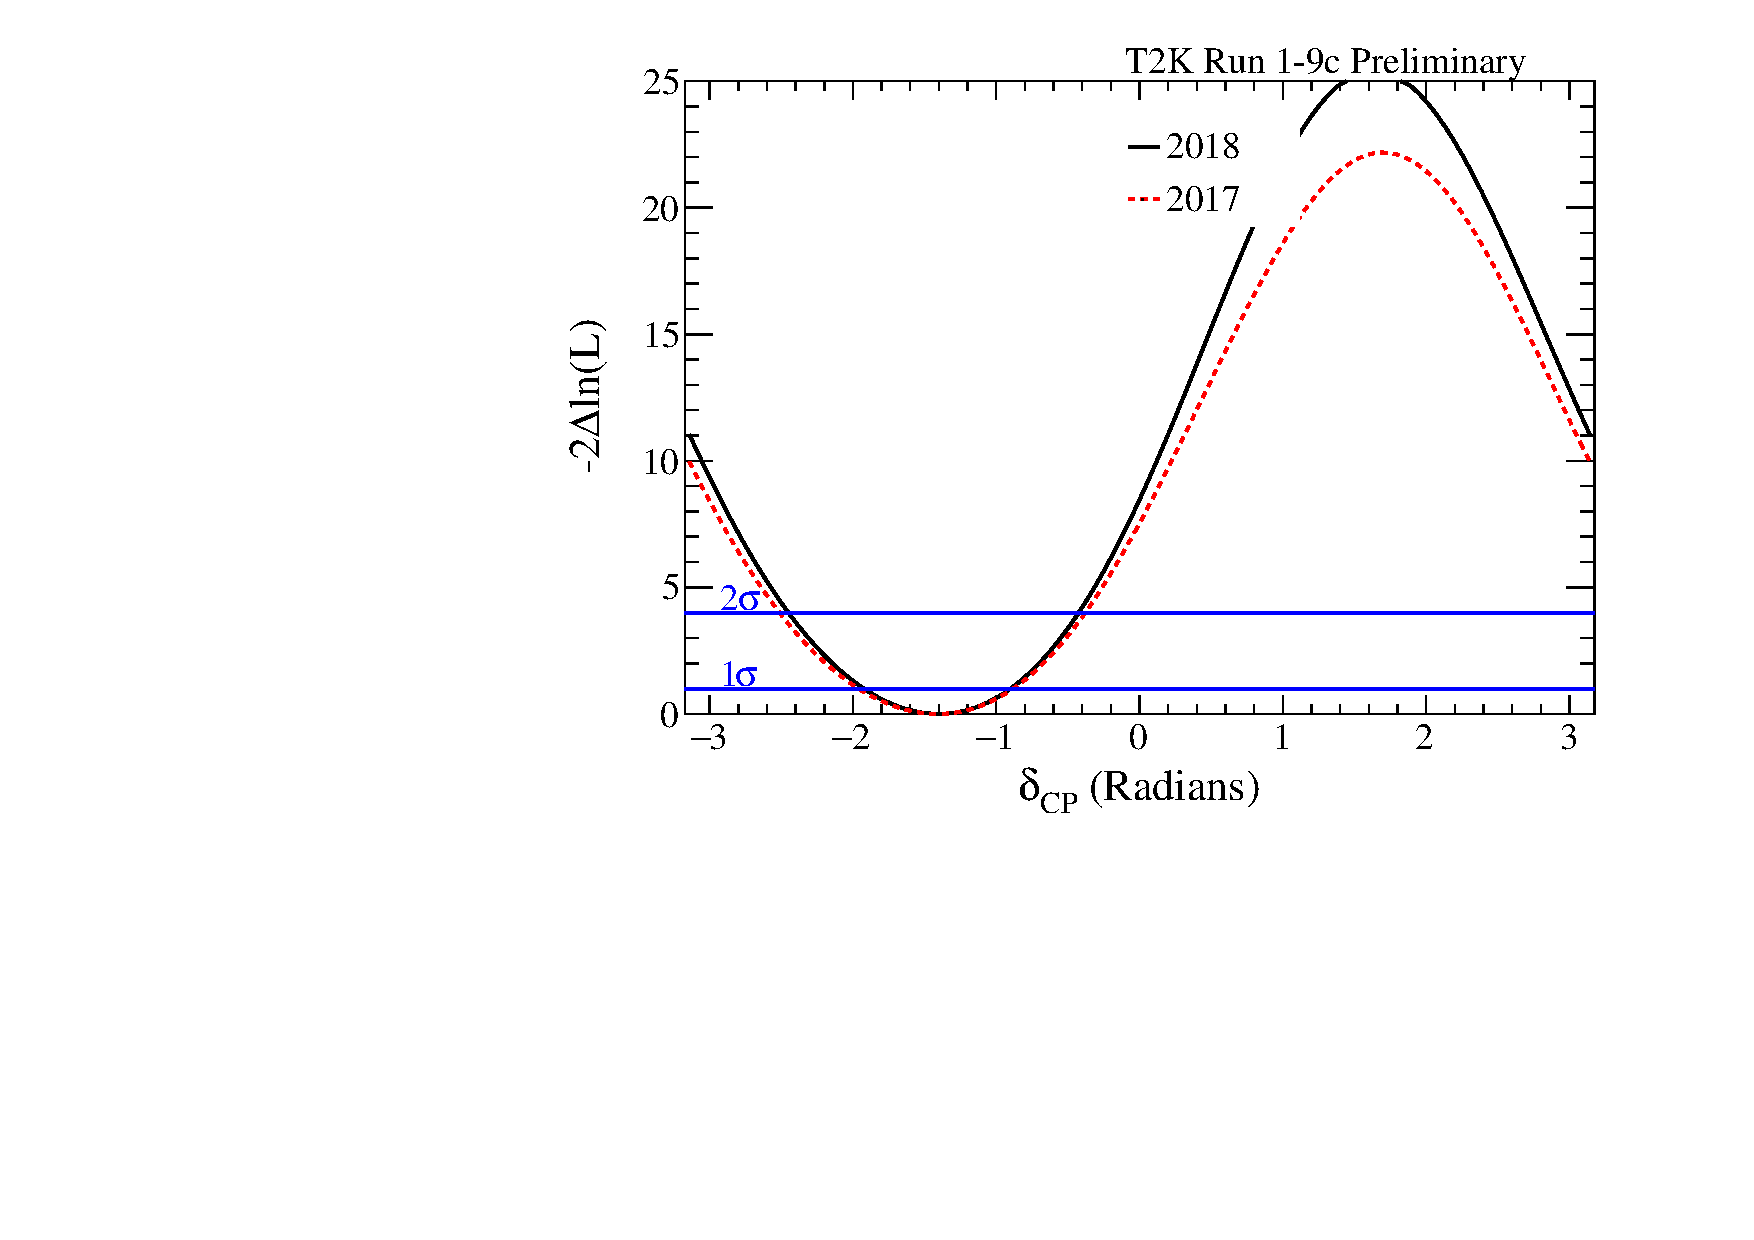
\includegraphics[width=0.9\textwidth]{images/data/comparison/deltacp_wrc_inverted_2018_v_2017}
		\caption{\deltacp IH with reactor constraint}
	\end{subfigure}
	\begin{subfigure}[b]{0.49\textwidth}
		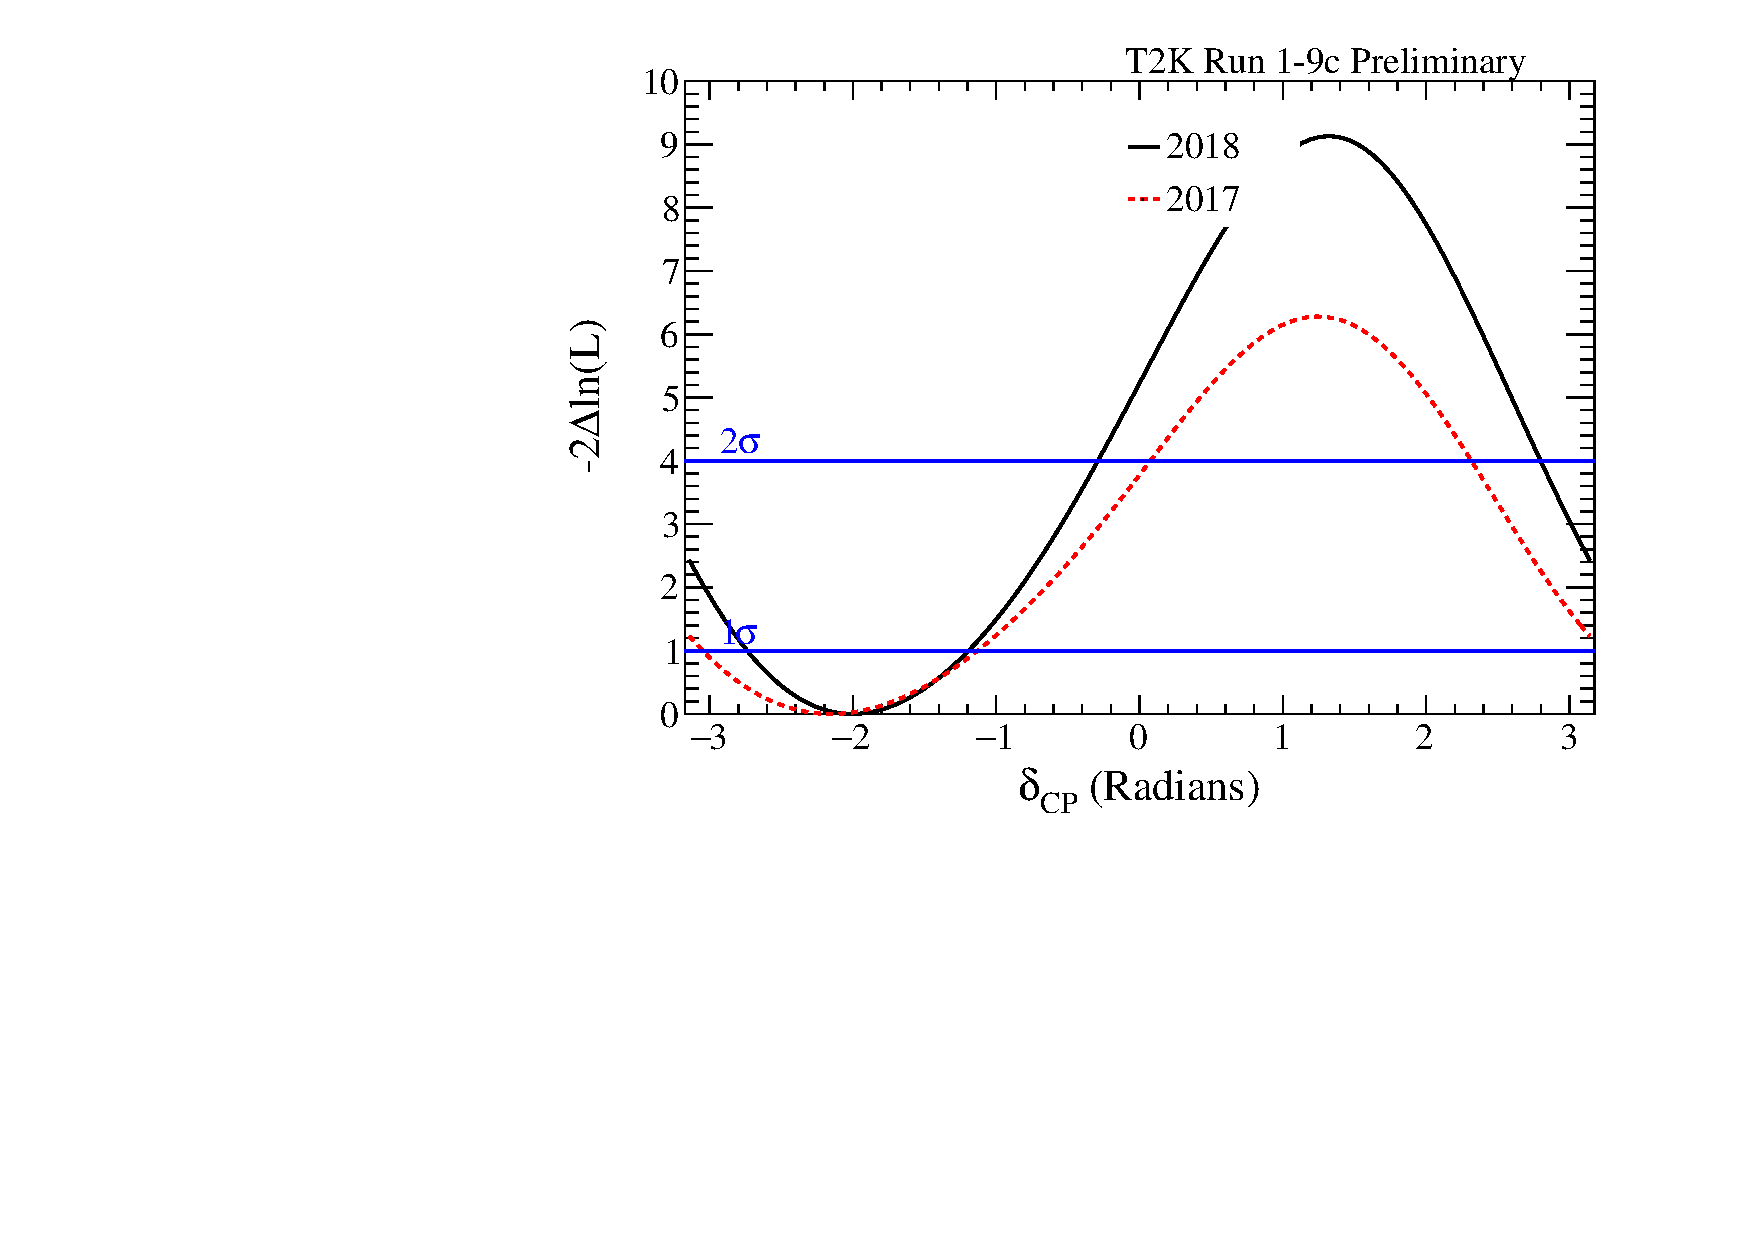
\includegraphics[width=0.9\textwidth]{images/data/comparison/deltacp_worc_normal_2018_v_2017}
		\caption{\deltacp NH without reactor constraint}
	\end{subfigure}
	\begin{subfigure}[b]{0.49\textwidth}
		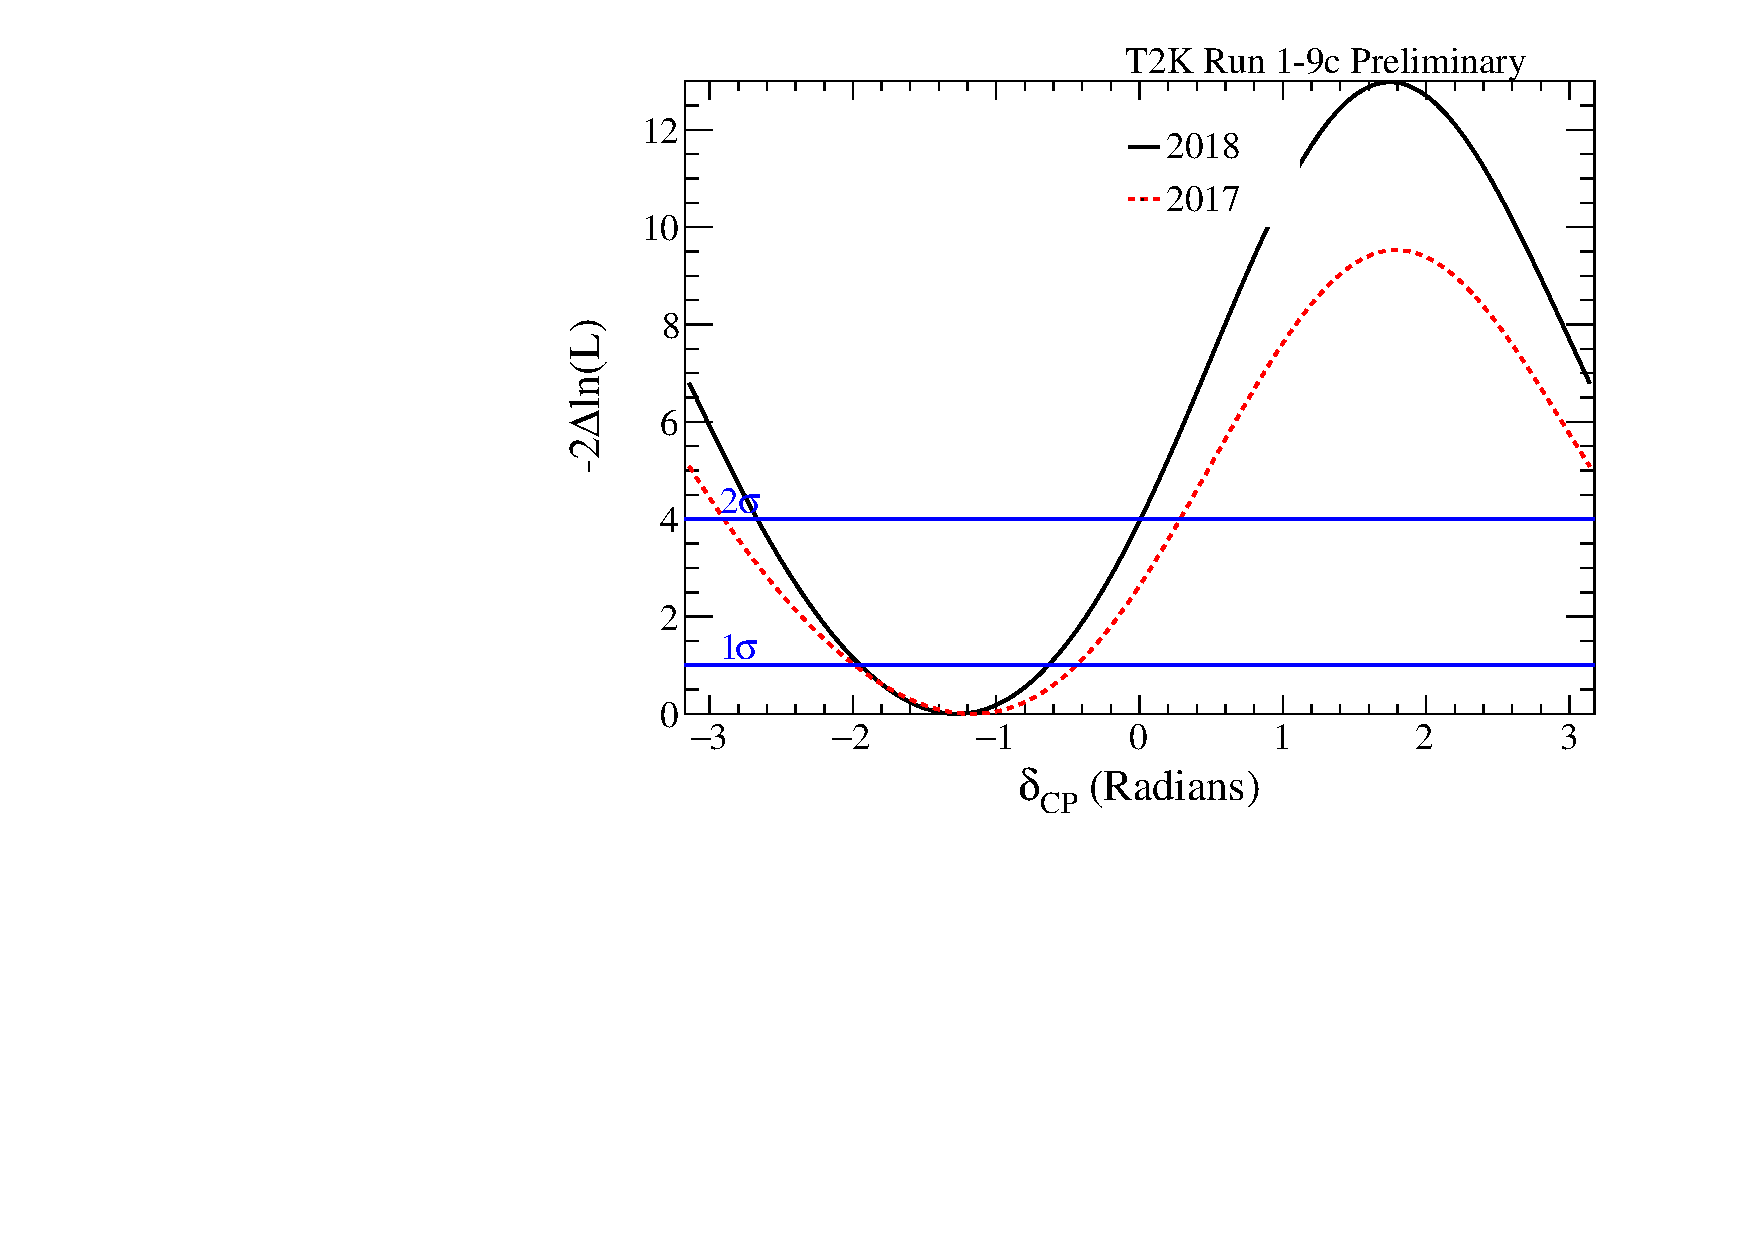
\includegraphics[width=0.9\textwidth]{images/data/comparison/deltacp_worc_inverted_2018_v_2017}
		\caption{\deltacp IH without reactor constraint}
	\end{subfigure}
	\caption {
		The expected $\Delta\chi^2$ distribution as a function of \deltacp with and without reactor constraint. Normal and inverted hierarchy contours are independent. All 5 samples were used to produce these fits.
	}
	\label{fig:dcp_data_compare}
\end{figure*}
\clearpage

\subsection{Results for \ssqthonethree}

The result for \ssqthonethree (without reactor constraint) is shown in fig.~\ref{fig:th13_data_compare}. A small shift in the best-fit value can be observed, along with a tightening of the contour.

\begin{figure*}[htb]
	\center
	\begin{subfigure}[b]{0.49\textwidth}
		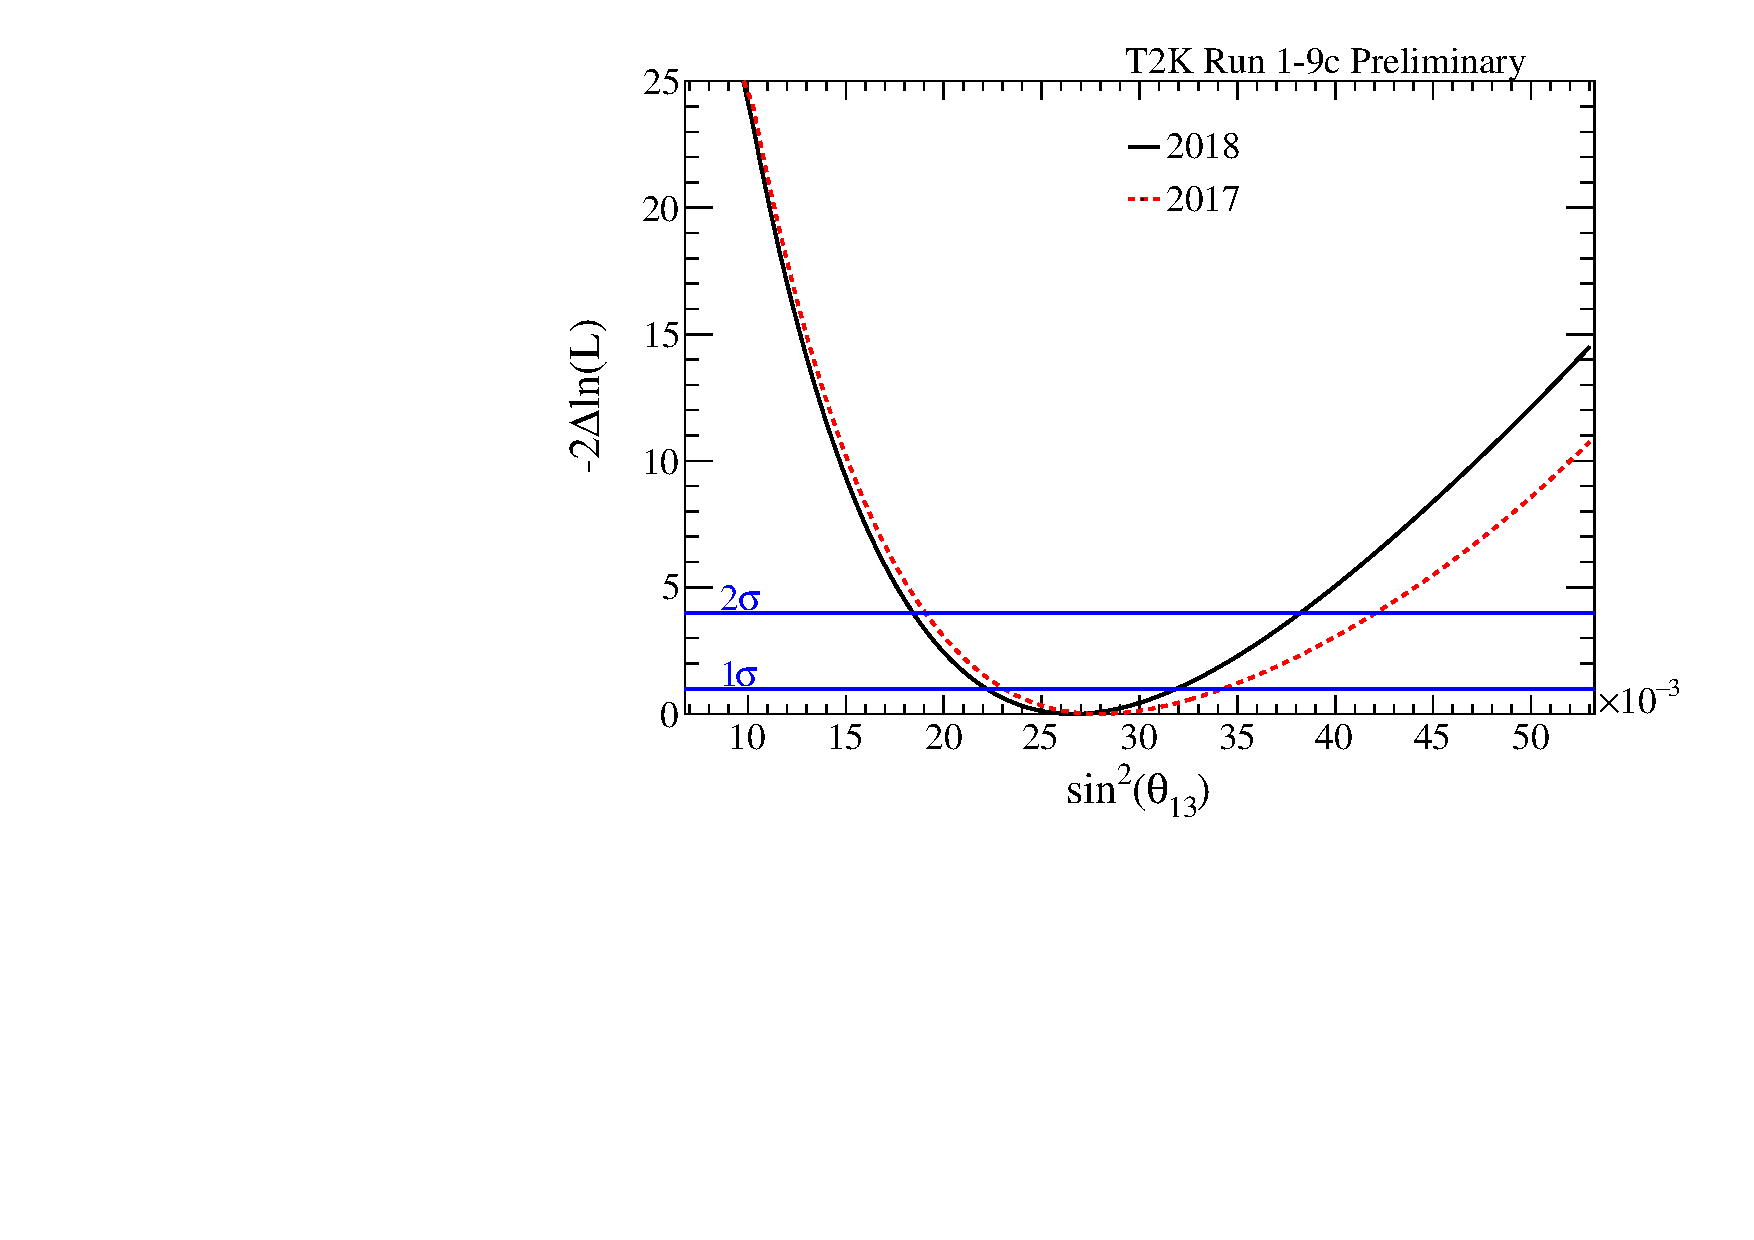
\includegraphics[width=0.9\textwidth]{images/data/comparison/theta13_worc_normal_2018_v_2017}
		\caption{\ssqthonethree NH without reactor constraint}
	\end{subfigure}
	\begin{subfigure}[b]{0.49\textwidth}
		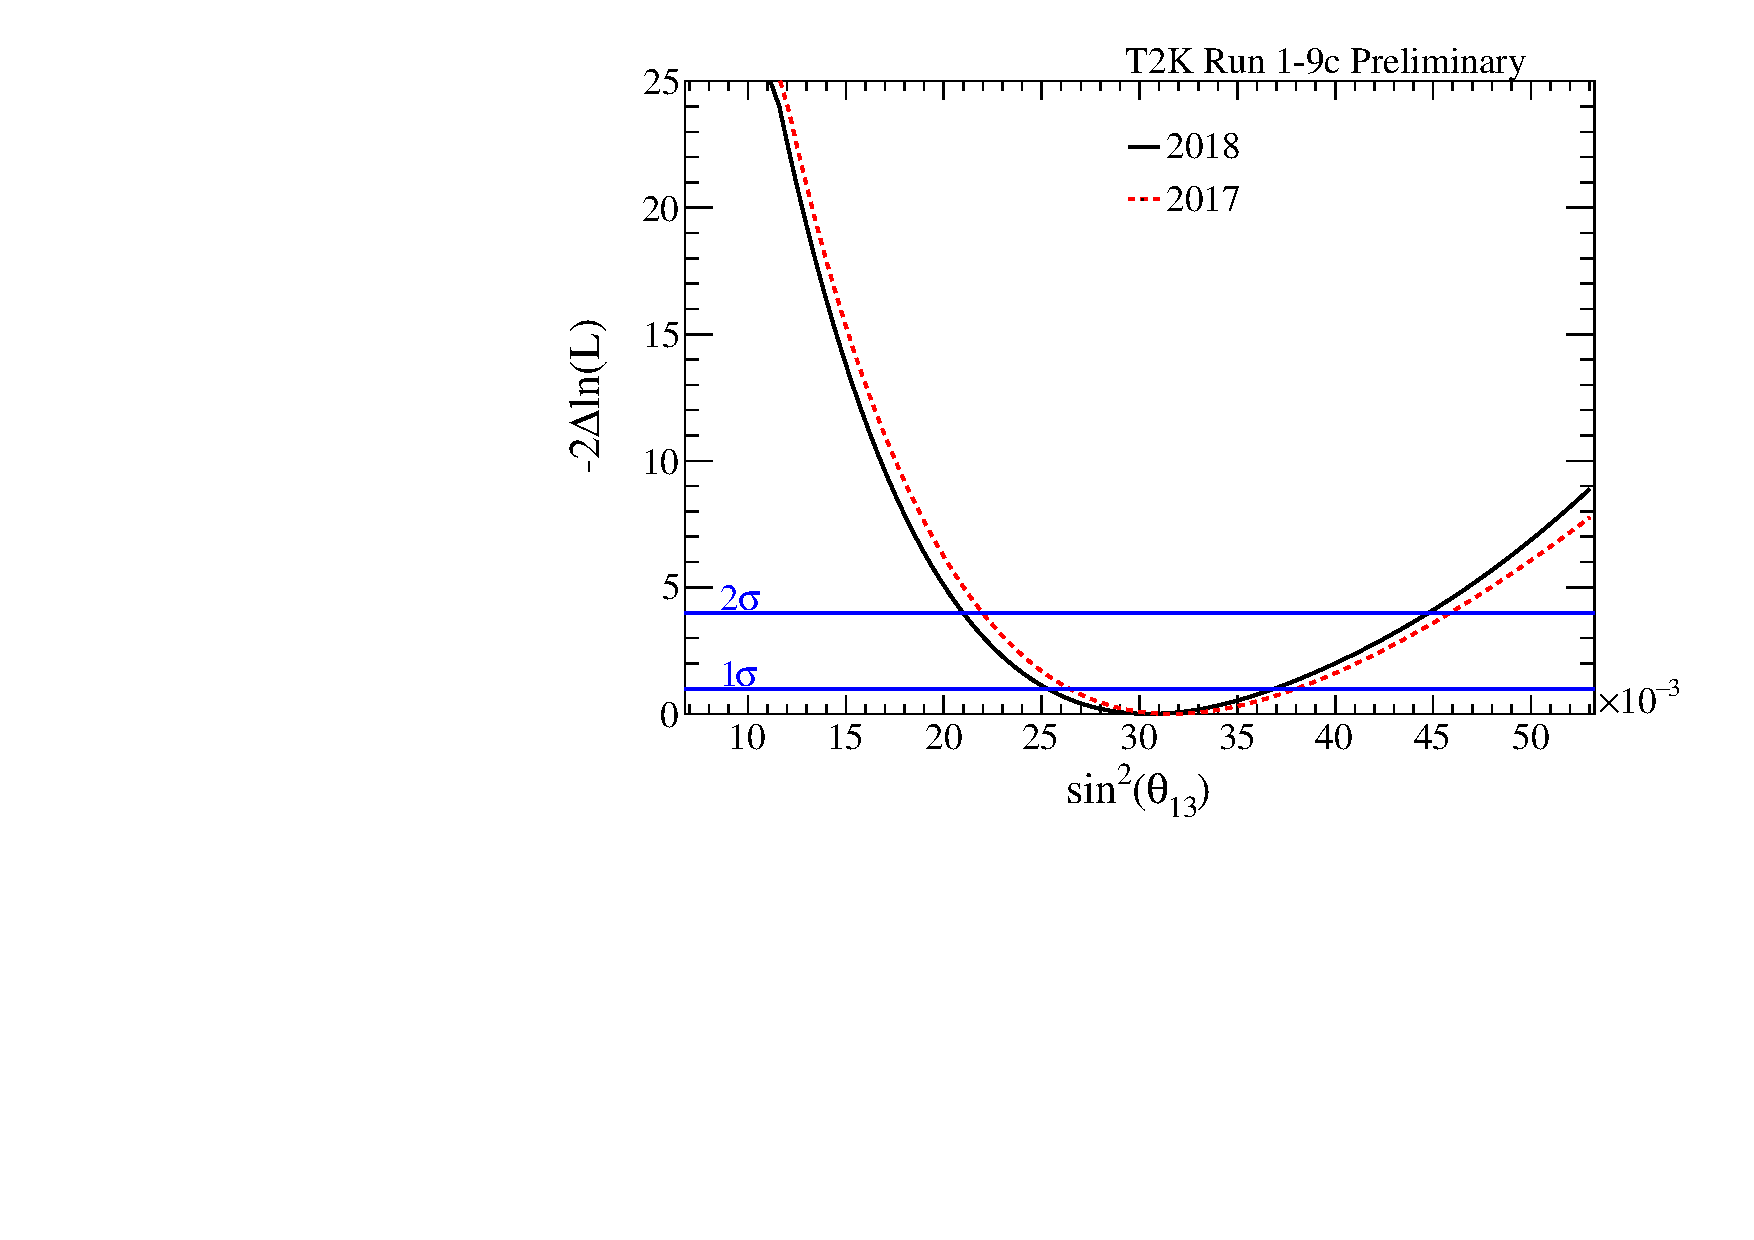
\includegraphics[width=0.9\textwidth]{images/data/comparison/theta13_worc_inverted_2018_v_2017}
		\caption{\ssqthonethree IH without reactor constraint}
	\end{subfigure}
	\caption {
		The expected $\Delta\chi^2$ distribution as a function of \ssqthonethree without reactor constraint. Normal and inverted hierarchy contours are independent. All 5 samples were used to produce these fits.
	}
	\label{fig:th13_data_compare}
\end{figure*}

\clearpage

\subsection{Results for \ssqthtwothree}

The result for \ssqthtwothree with reactor constraint and T2K only is shown in fig.~\ref{fig:th23_data_compare}. As noted for the appearance fit, the best-fit values for \ssqthtwothree have shifted away from maximal disappearance.

\begin{figure*}[htb]
	\center
	\begin{subfigure}[b]{0.49\textwidth}
		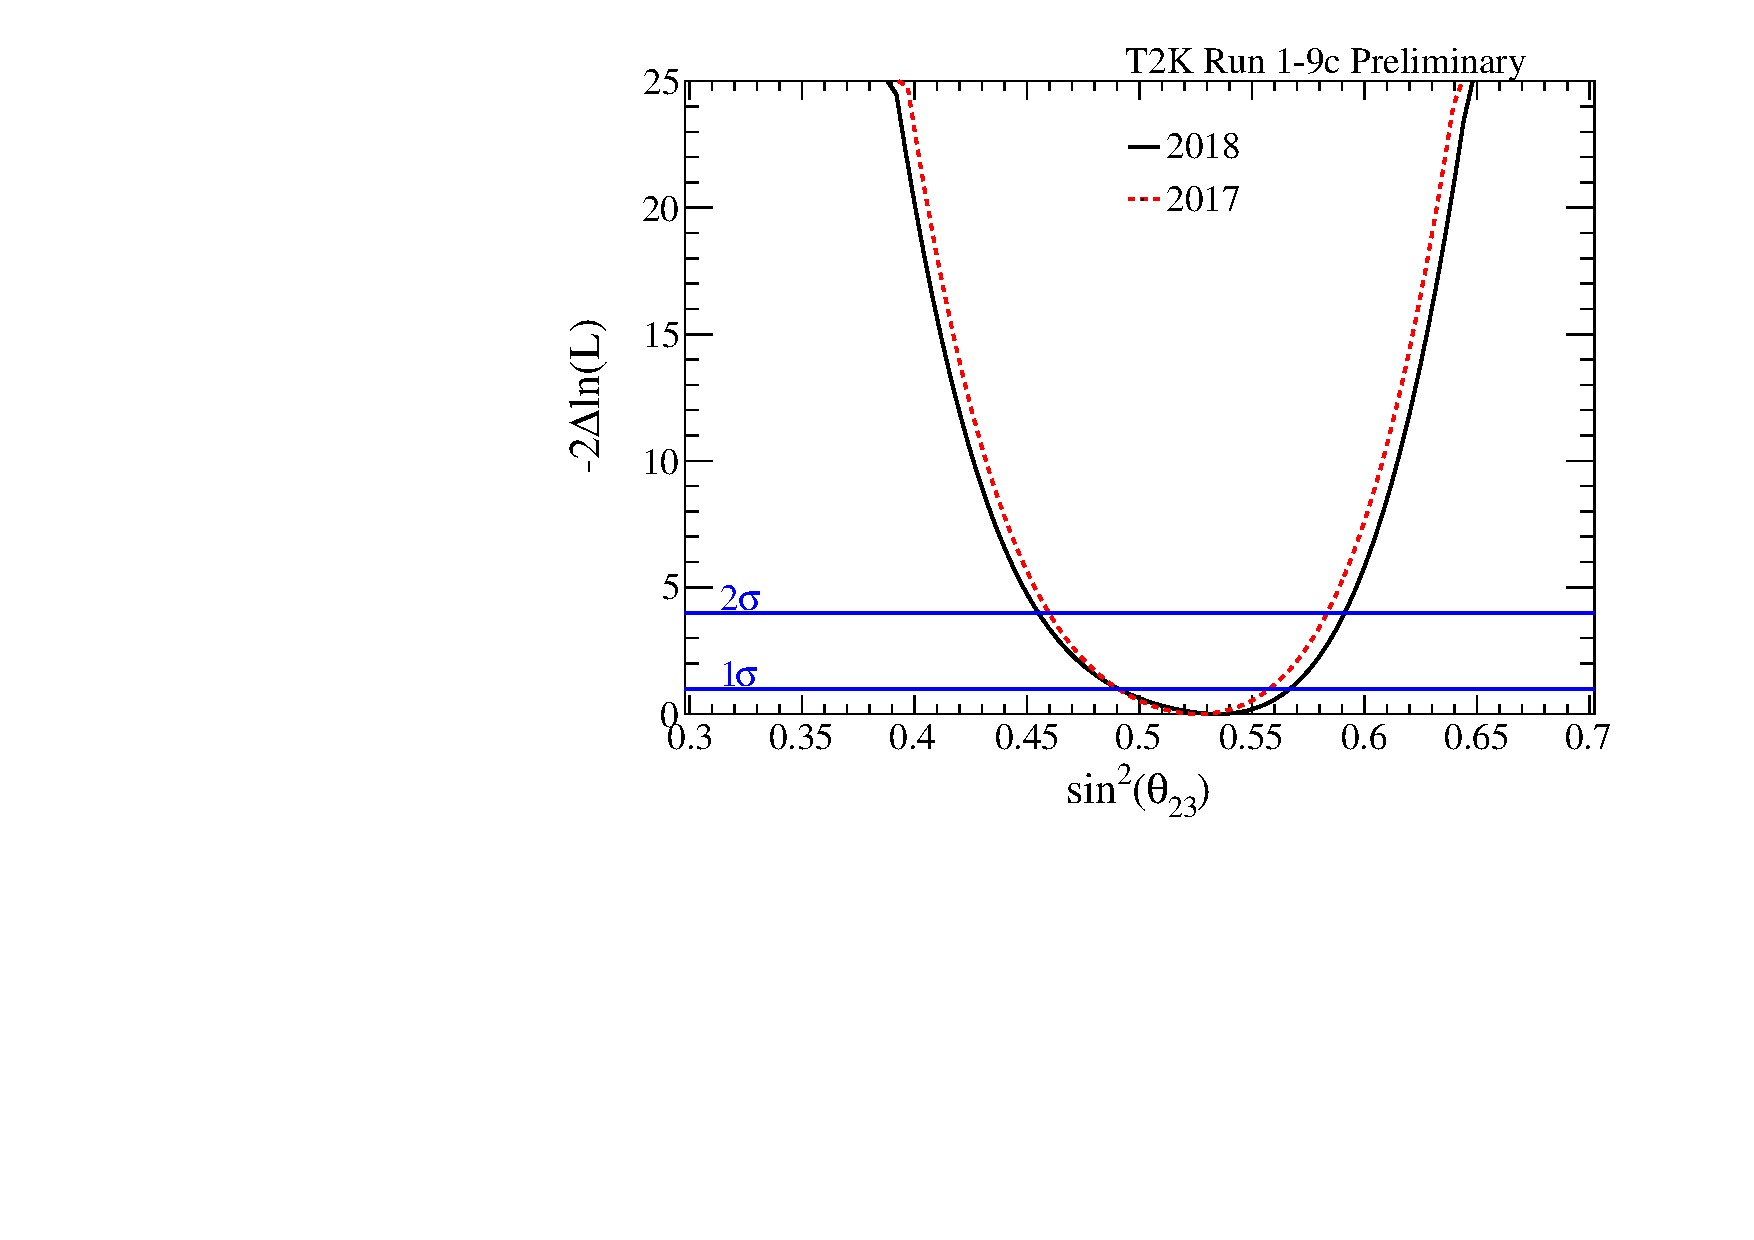
\includegraphics[width=0.9\textwidth]{images/data/comparison/theta23_wrc_normal_2018_v_2017}
		\caption{\ssqthtwothree NH with reactor constraint}
	\end{subfigure}
	\begin{subfigure}[b]{0.49\textwidth}
		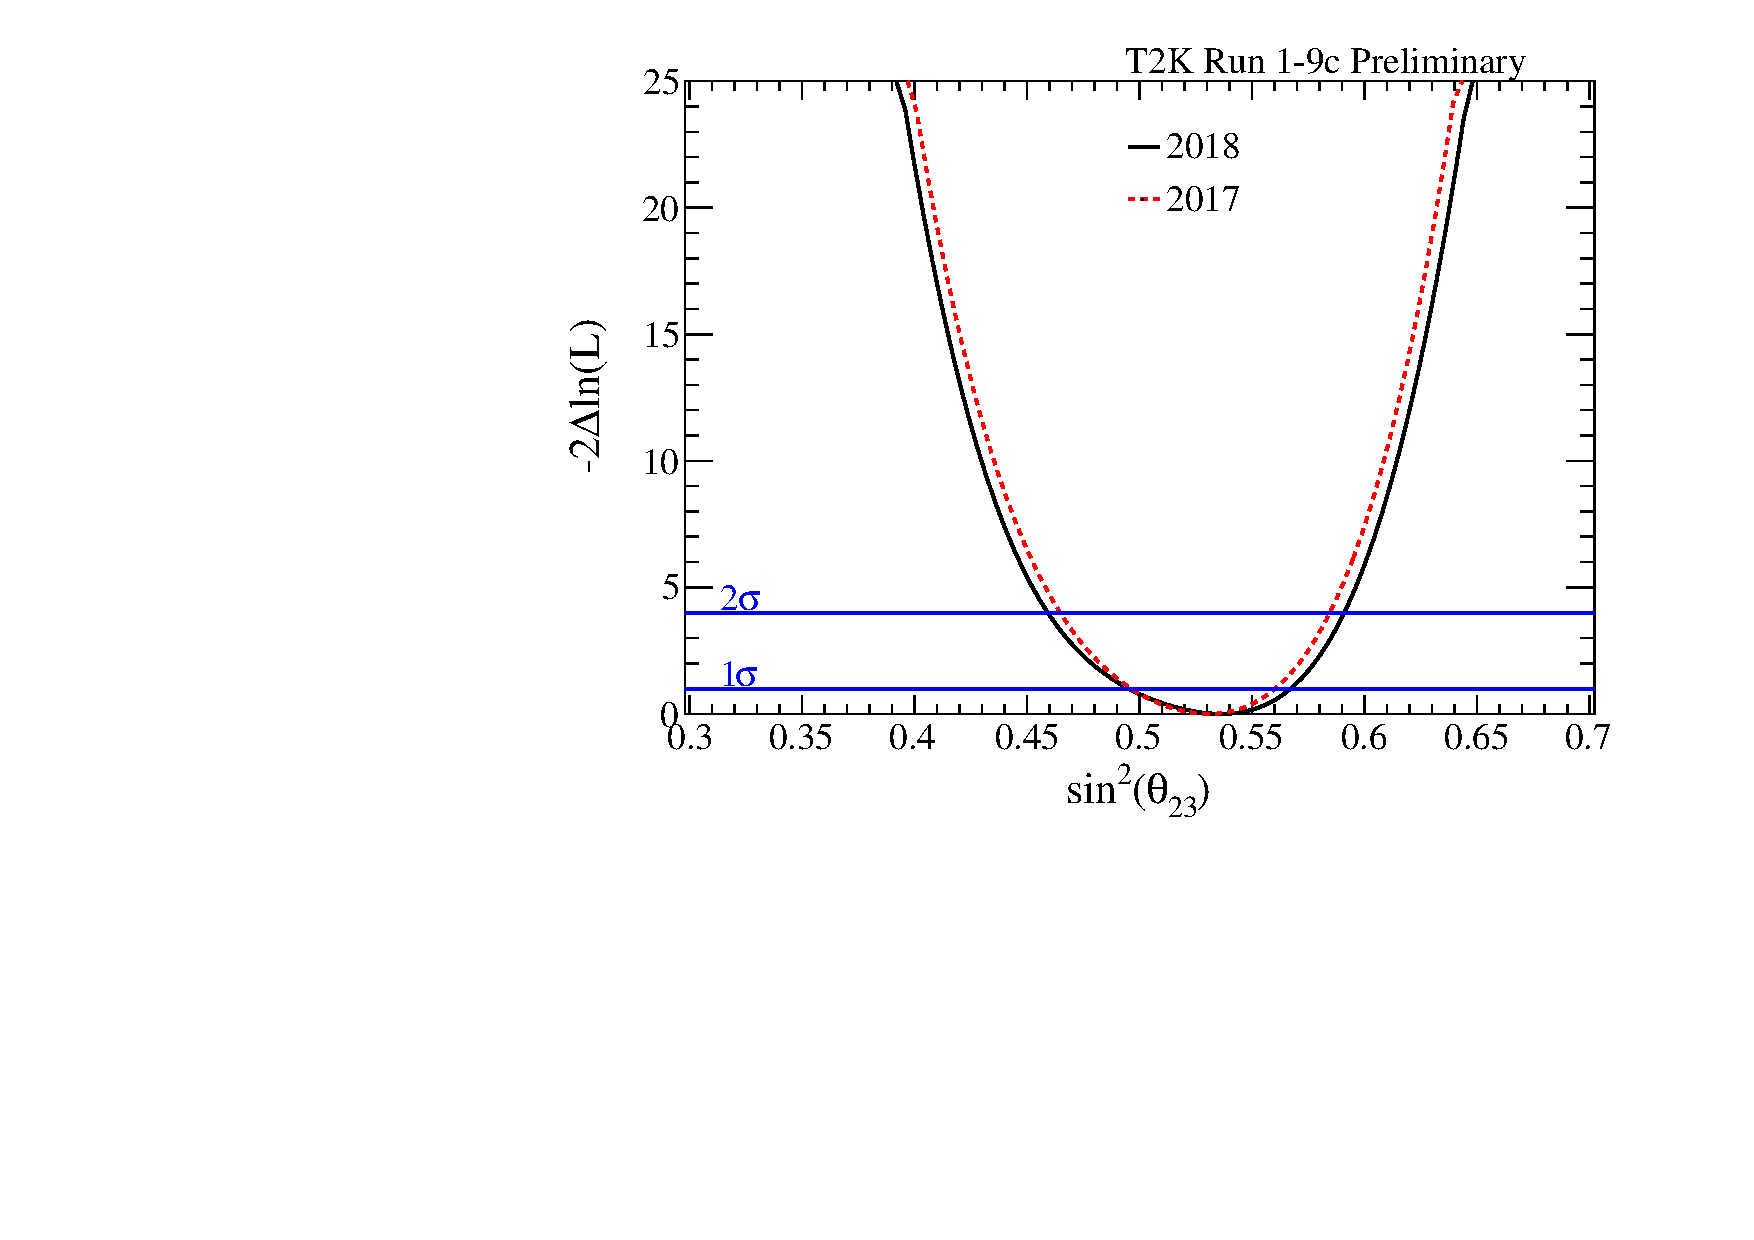
\includegraphics[width=0.9\textwidth]{images/data/comparison/theta23_wrc_inverted_2018_v_2017}
		\caption{\ssqthtwothree IH with reactor constraint}
	\end{subfigure}
	\begin{subfigure}[b]{0.49\textwidth}
		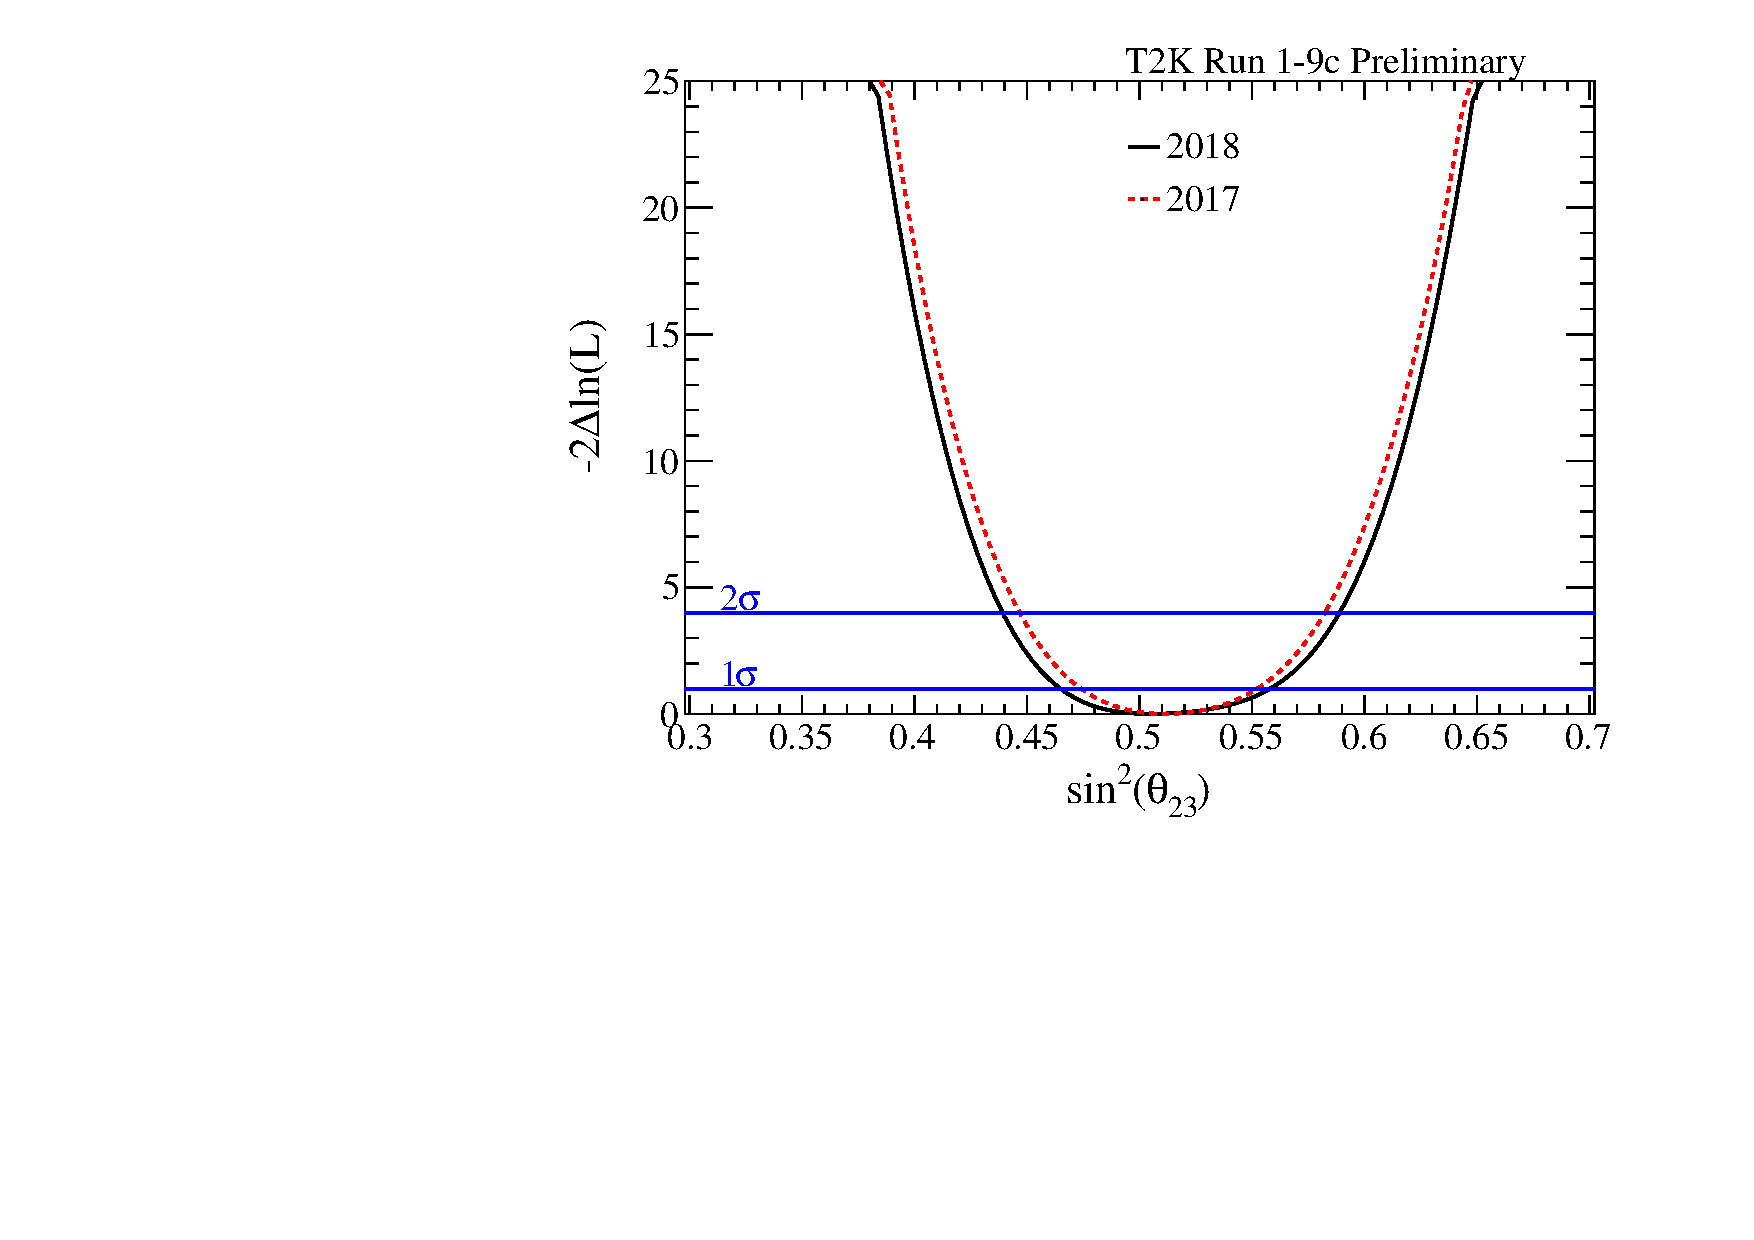
\includegraphics[width=0.9\textwidth]{images/data/comparison/theta23_worc_normal_2018_v_2017}
		\caption{\ssqthtwothree NH without reactor constraint}
	\end{subfigure}
	\begin{subfigure}[b]{0.49\textwidth}
		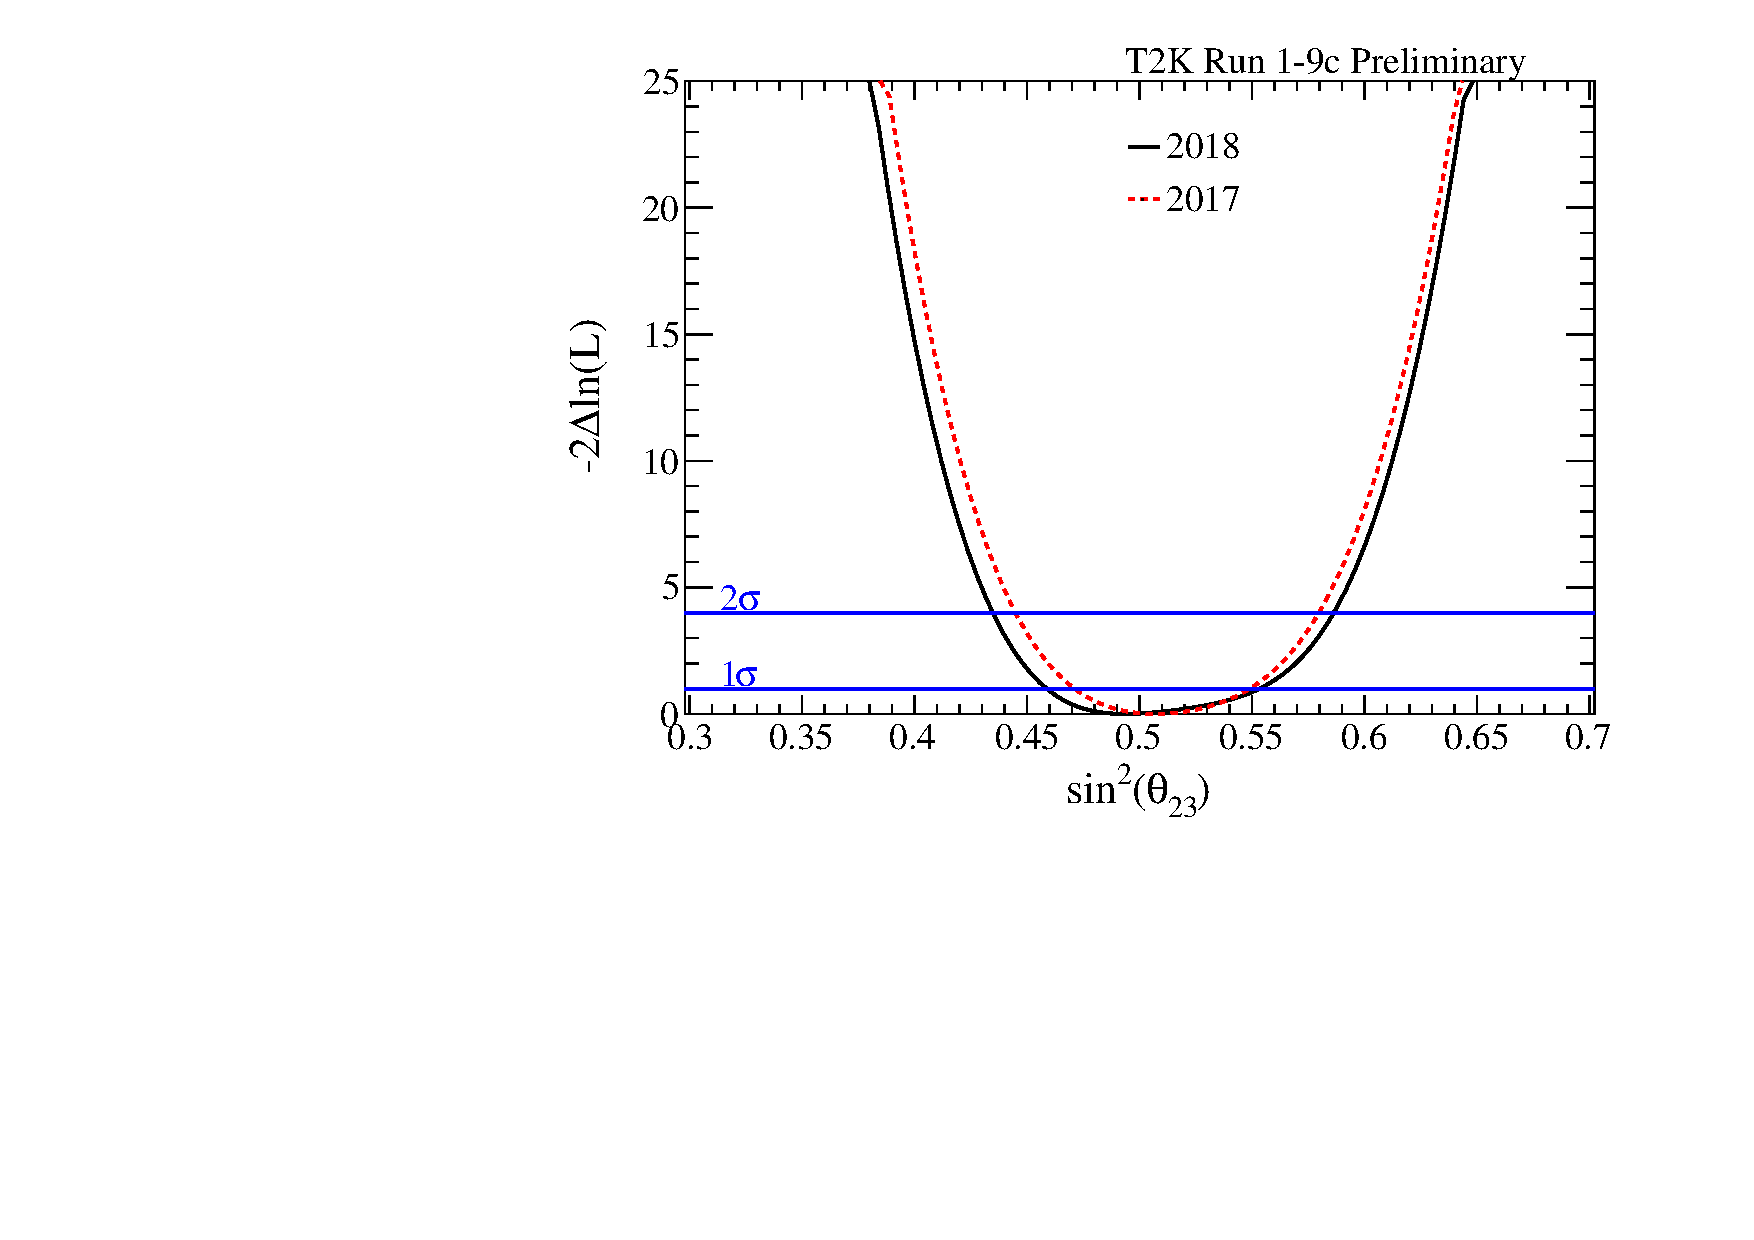
\includegraphics[width=0.9\textwidth]{images/data/comparison/theta23_worc_inverted_2018_v_2017}
		\caption{\ssqthtwothree IH without reactor constraint}
	\end{subfigure}
	\caption {
		The expected $\Delta\chi^2$ distribution as a function of \ssqthtwothree with and without reactor constraint. Normal and inverted hierarchy contours are independent. All 5 samples were used to produce these fits.
	}
	\label{fig:th23_data_compare}
\end{figure*}
\clearpage

\subsection{Results for \dmsq}

The result for \dmsq with reactor constraint and T2K only is shown in fig.~\ref{fig:dmsq_data_compare}. The \RunPeriod data favour lower values of \dmsq relative to \PrevRunPeriod, though the overall width of the contour is largely unchanged.

\begin{figure*}[htb]
	\center
	\begin{subfigure}[b]{0.49\textwidth}
		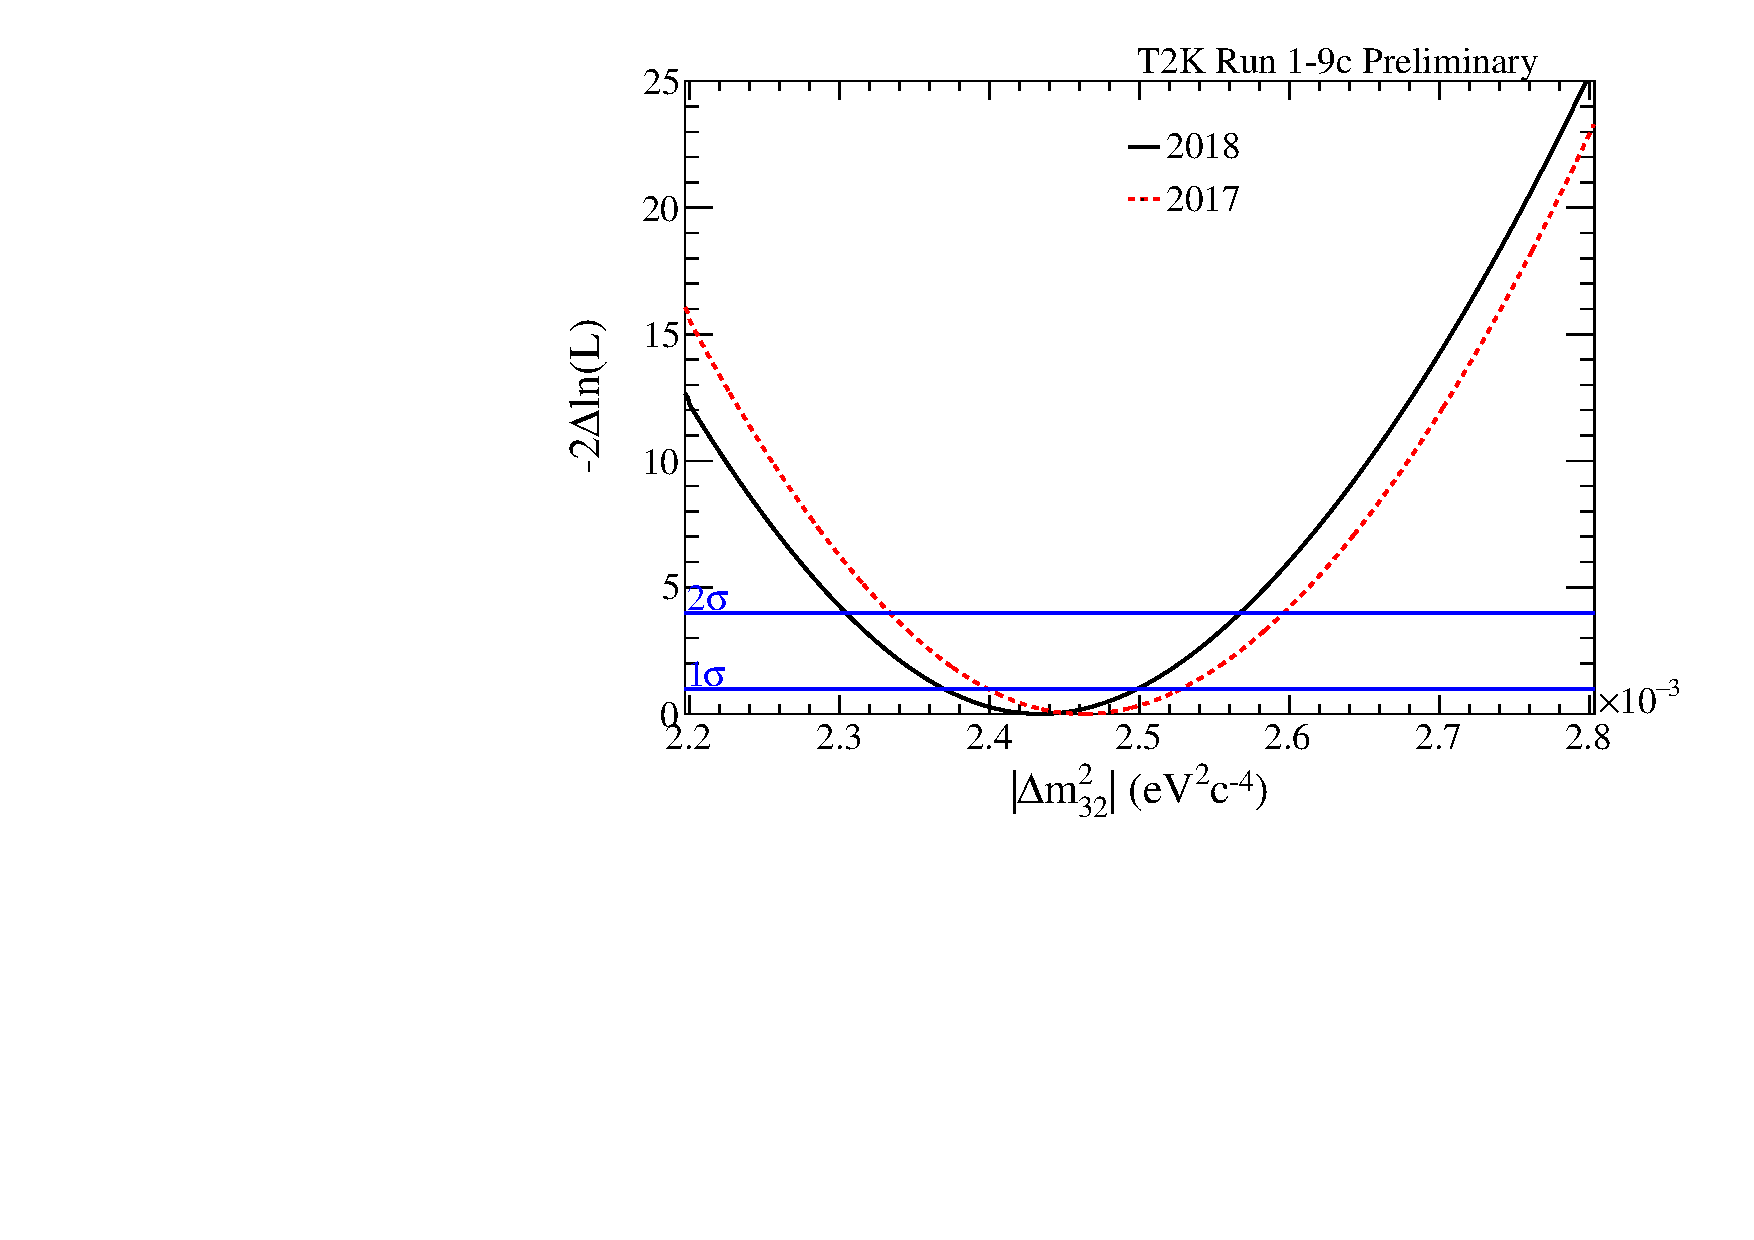
\includegraphics[width=0.9\textwidth]{images/data/comparison/dmsq_wrc_normal_2018_v_2017}
		\caption{\dmsq NH with reactor constraint}
	\end{subfigure}
	\begin{subfigure}[b]{0.49\textwidth}
		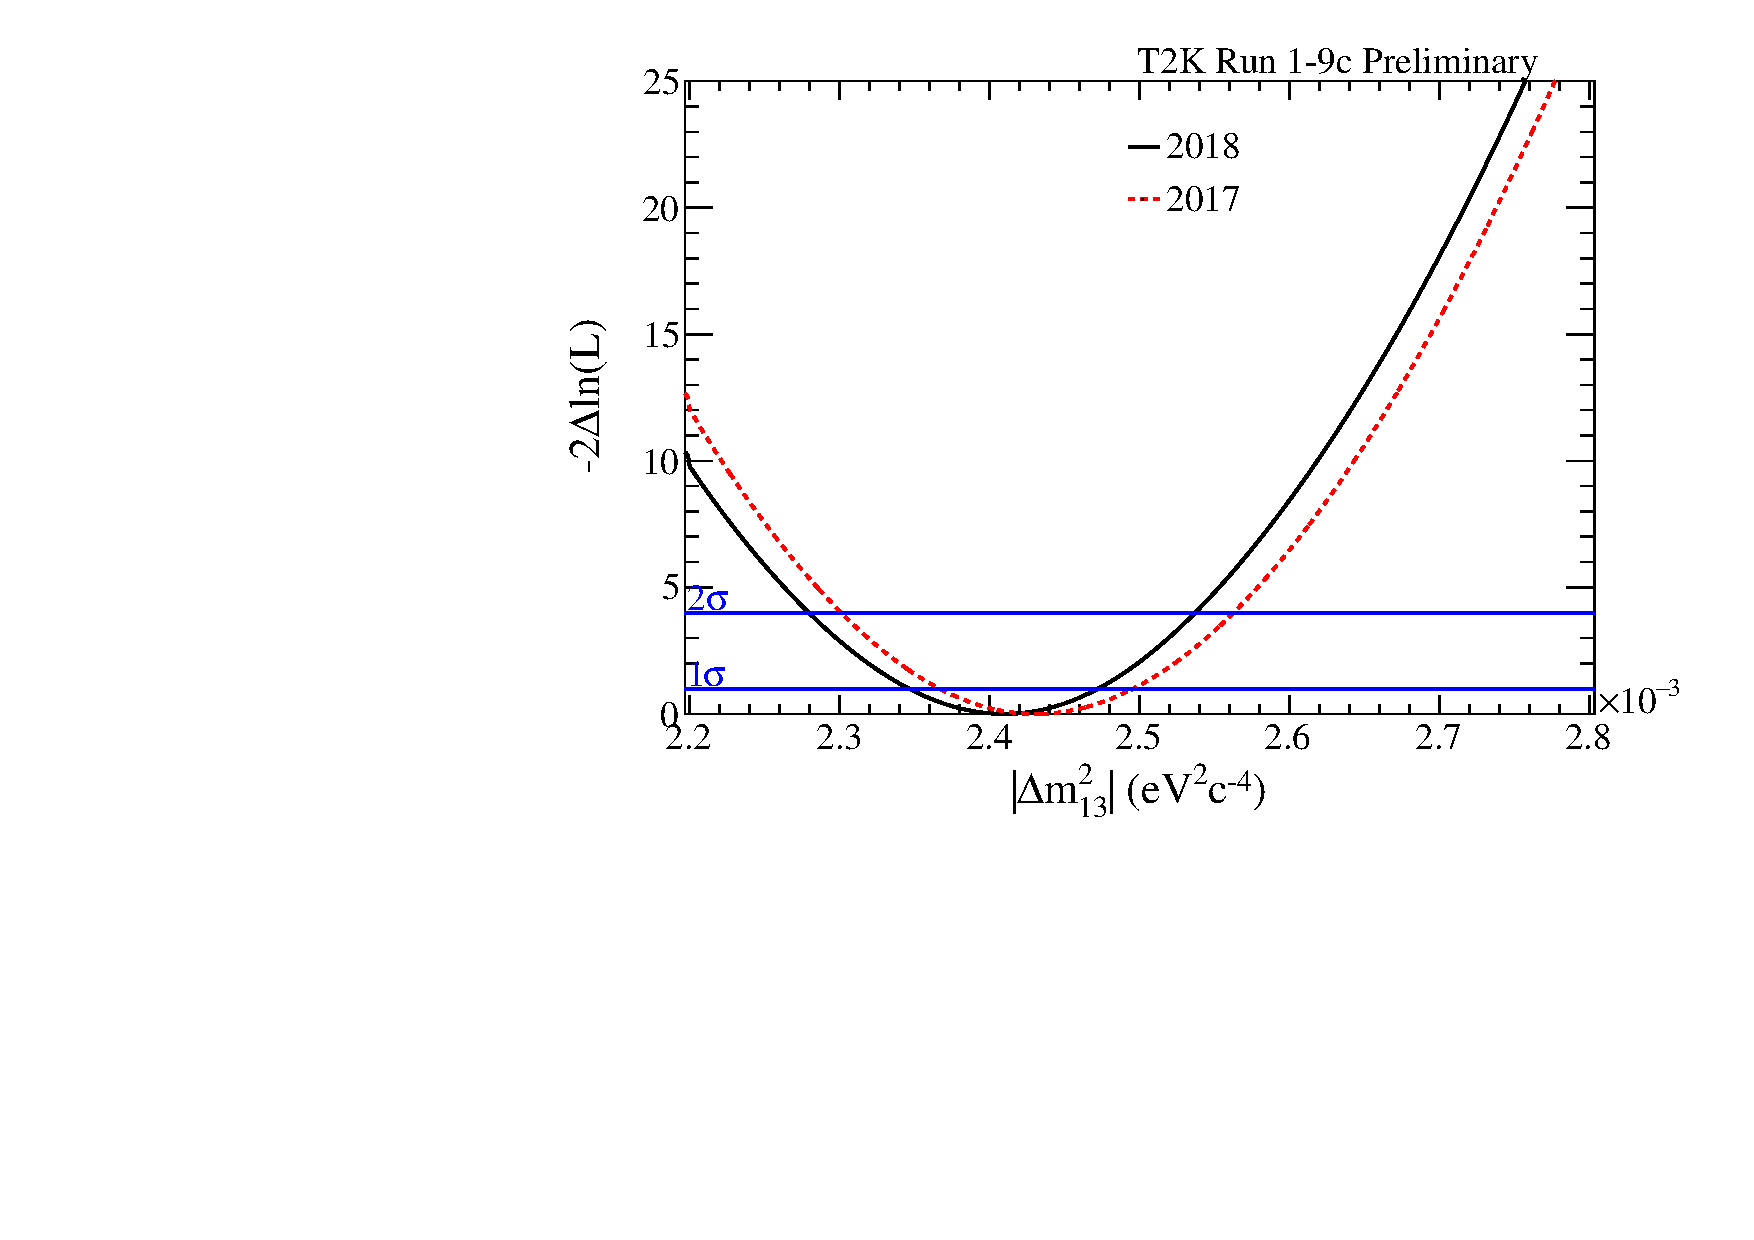
\includegraphics[width=0.9\textwidth]{images/data/comparison/dmsq_wrc_inverted_2018_v_2017}
		\caption{\dmsq IH with reactor constraint}
	\end{subfigure}
	\begin{subfigure}[b]{0.49\textwidth}
		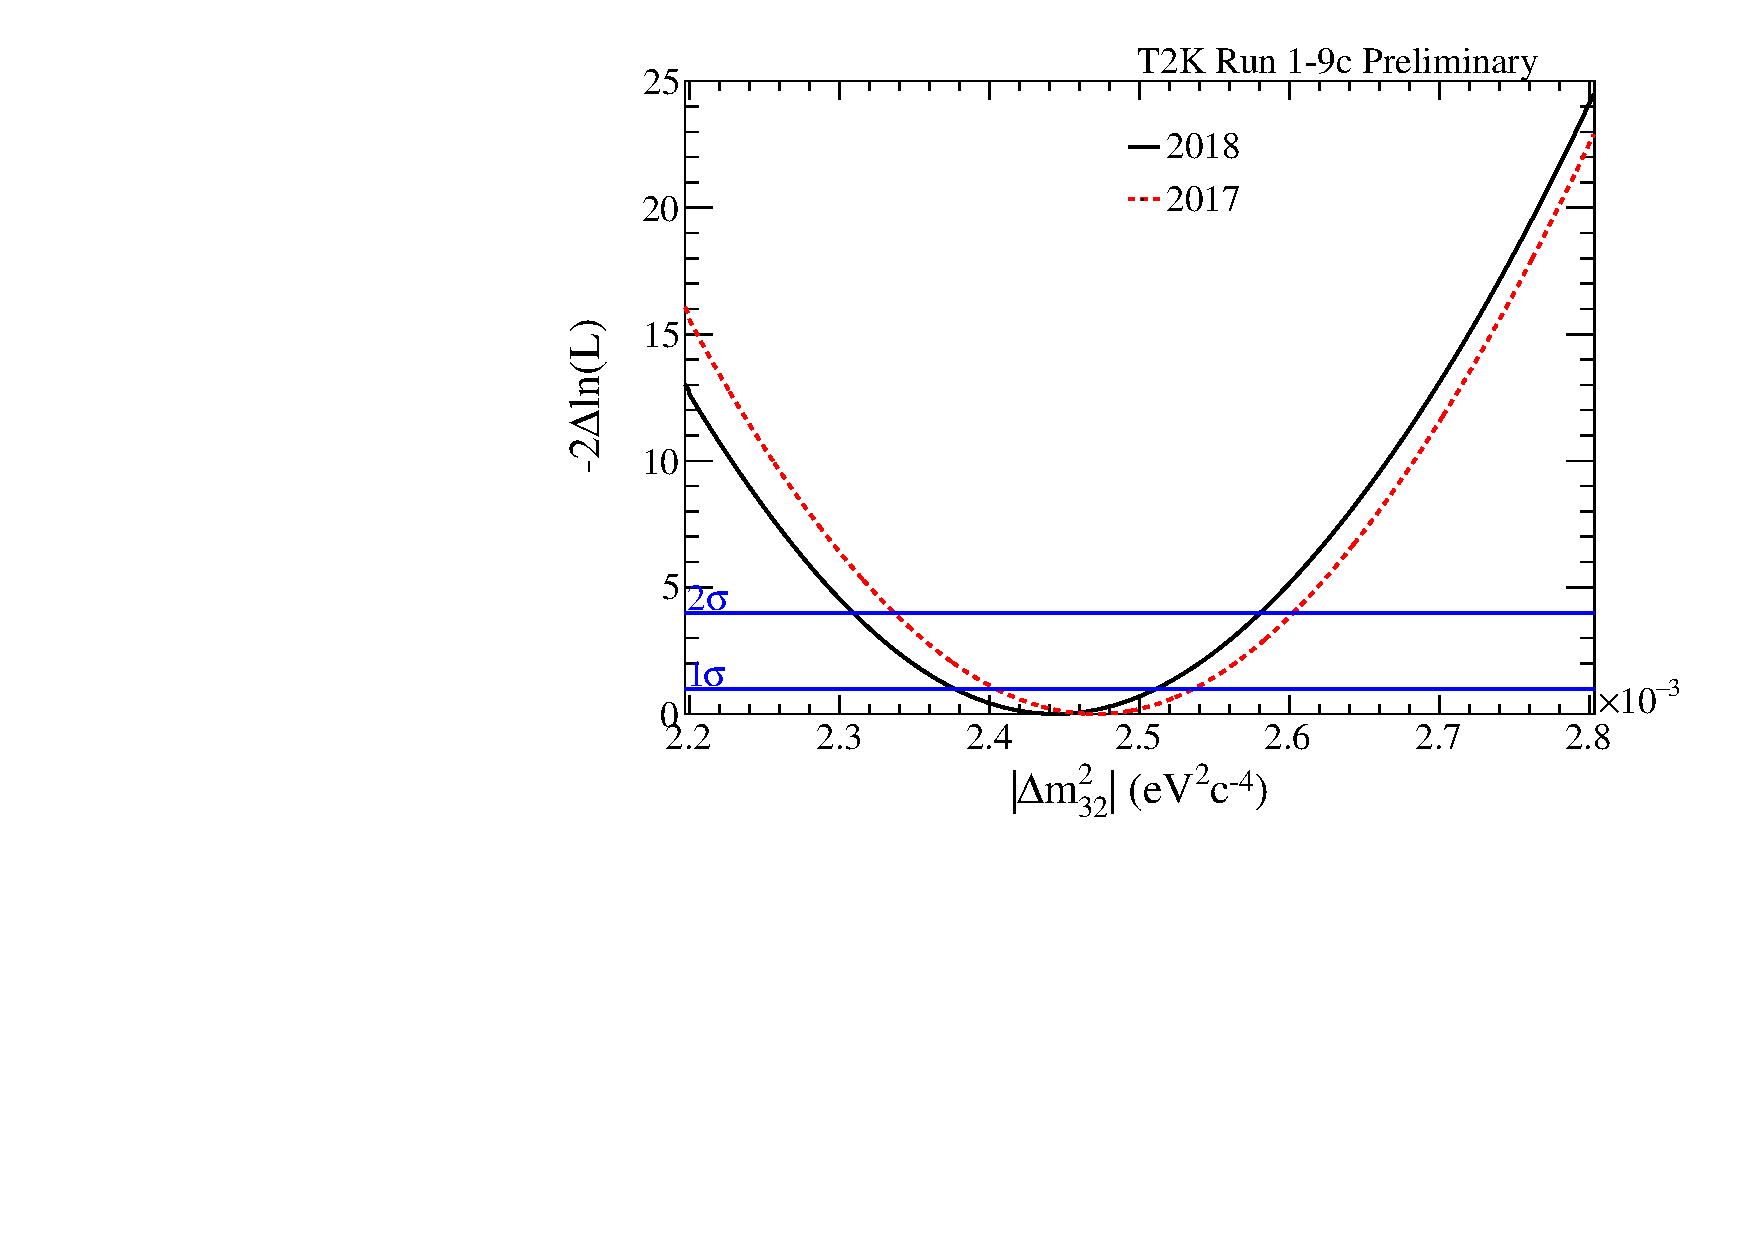
\includegraphics[width=0.9\textwidth]{images/data/comparison/dmsq_worc_normal_2018_v_2017}
		\caption{\dmsq NH without reactor constraint}
	\end{subfigure}
	\begin{subfigure}[b]{0.49\textwidth}
		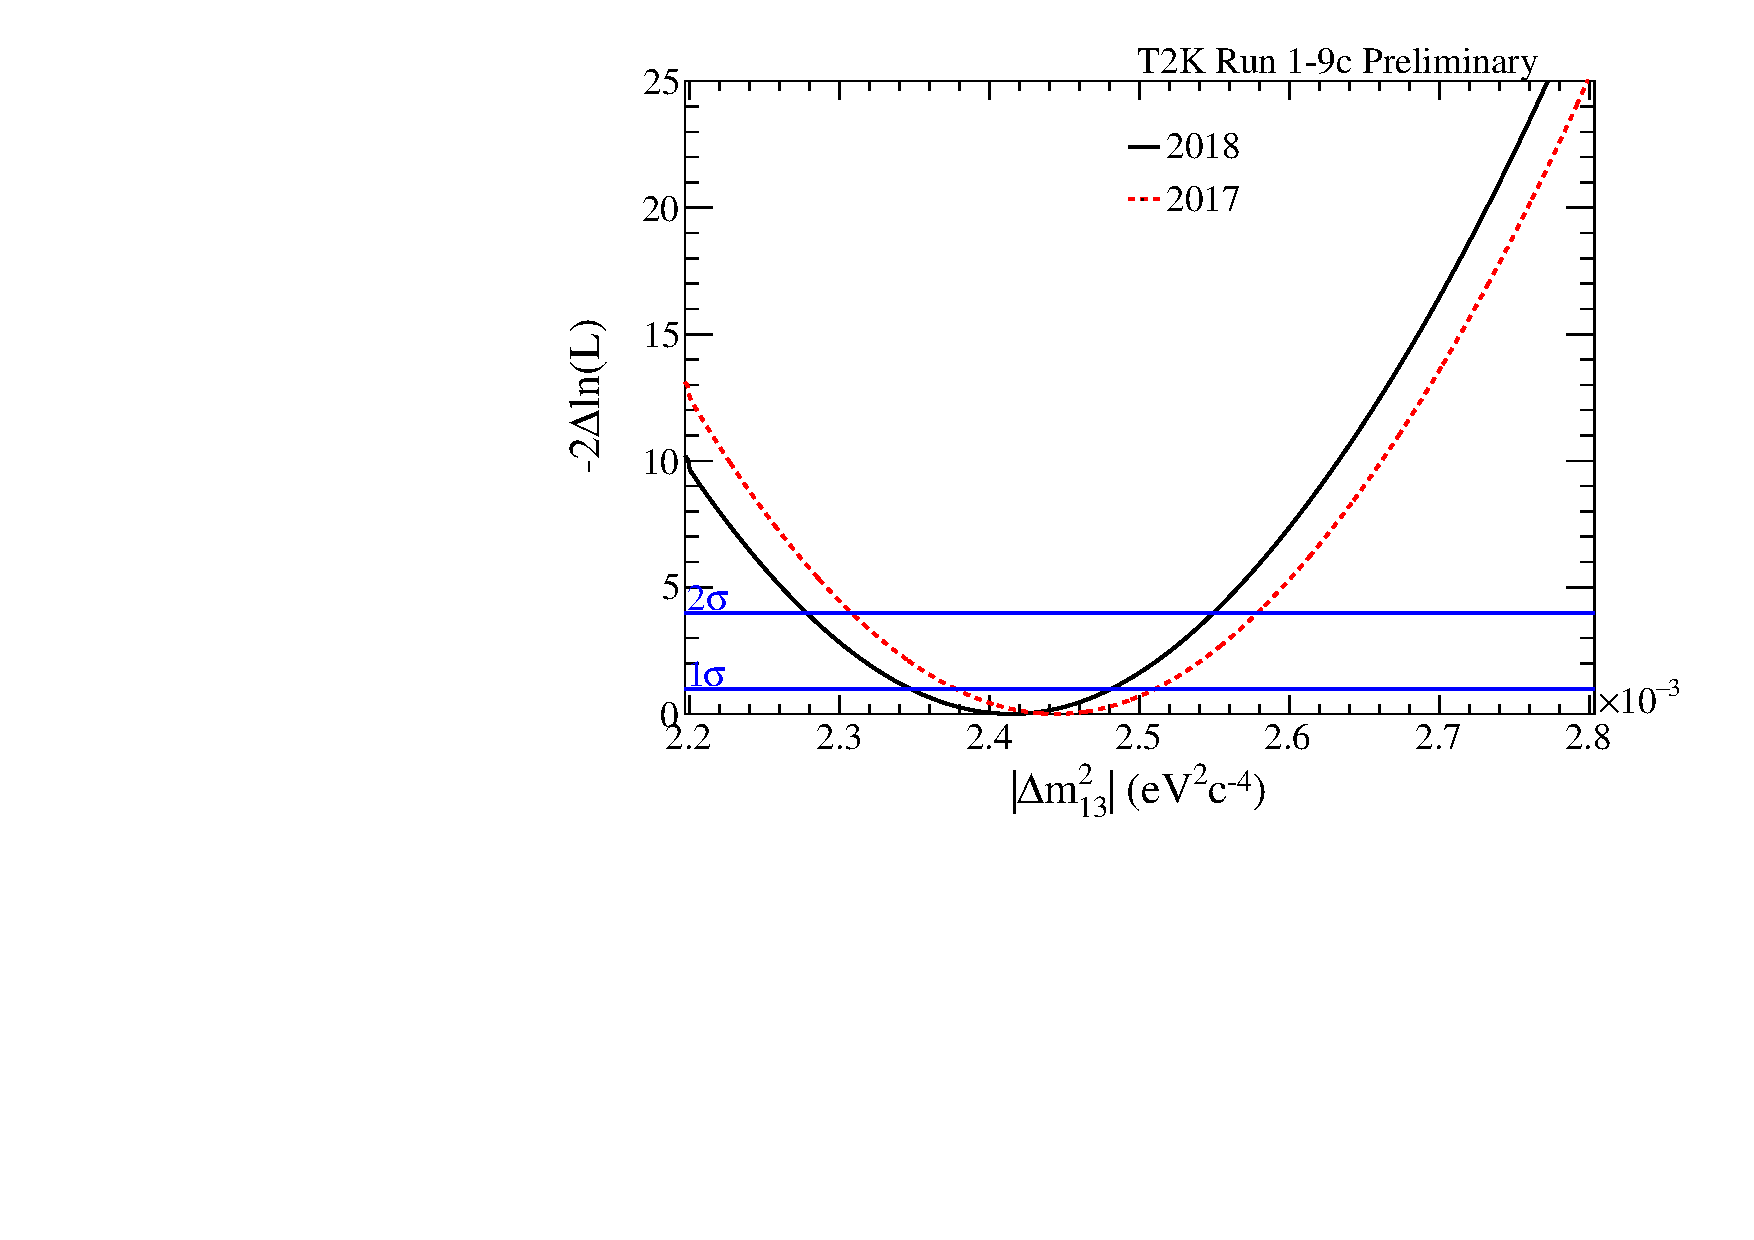
\includegraphics[width=0.9\textwidth]{images/data/comparison/dmsq_worc_inverted_2018_v_2017}
		\caption{\dmsq IH without reactor constraint}
	\end{subfigure}
	\caption {
		The expected $\Delta\chi^2$ distribution as a function of \dmsqtwothree with and without reactor constraint. Normal and inverted hierarchy contours are independent. All 5 samples were used to produce these fits.
	}
	\label{fig:dmsq_data_compare}
\end{figure*}

\clearpage
\clearpage

% --------------------------------------------------------------------------------------------

\section{Summary}
\label{sec:summary}

In this technical note, we have presented the results of the 3-flavour $\bar{\nu}/\nu$ joint analysis performed by the {\em VALOR} group, on the combined \RunPeriod data set. The goal of the analysis was to search for CP violation in the leptonic sector and determine limits on \deltacp as well as measure all the other oscillation parameters to which T2K is sensitive: \ssqthonethree, \ssqthtwothree, \dmsqtwothree (\dmsqonethree) and partially mass hierarchy, to which T2K has little sensitivity.

This analysis predicts
\NskOscExpectationNumu{} $\pm$ \NskOscExpectationNumuError{} (syst) for neutrino $\mu$-like, \NskOscExpectationNumuBar{} $\pm$ \NskOscExpectationNumuBarError{} (syst) for antineutrino $\mu$-like, \NskOscExpectationNue{} $\pm$ \NskOscExpectationNueError{} (syst) for neutrino $e$-like, \NskOscExpectationNueBar{} $\pm$ \NskOscExpectationNueBarError{} (syst) for antineutrino $e$-like and \NskOscExpectationNueCConepi{} $\pm$ \NskOscExpectationNueCConepiError{} (syst) for neutrino \nueCConepi{} events in Super K and observes respectively \NskObservedNumu{} for neutrino $\mu$-like, \NskObservedNumuBar{}  for antineutrino $\mu$-like, \NskObservedNue{}  for neutrino $e$-like, \NskObservedNueBar{}  for antineutrino $e$-like and \NskObservedNueCConepi{} for neutrino \nueCConepi{}. 

The $\nu/\bar{\nu}$ analysis was performed in a framework of 3-flavour oscillations including matter effects in constant-density matter. The observed reconstructed energy spectrum of single $\mu$-like ring events and reconstructed energy versus lepton angle of single $e$-like ring events in addition to $e$-like events with an additional decay electron were used to compute the confidence intervals. All \NSyst{} systematic parameters as well as the oscillation parameters which were not parameters of interest considered in this analysis were marginalised.

From the fit of the \RunPeriod data we can see that the favoured value of \deltacp is \BestFitDeltacpwRC, close to $-\pi/2$. The Feldman-Cousins method is used to construct confidence intervals with neither over nor under coverage from which the significance to exclude the hypothesis of CP conservation is greater than 2 standard deviations.
\clearpage

%%% Local Variables:
%%% mode: latex
%%% TeX-master: "../TN327"
%%% End:


% References
\clearpage
%
% References
%

\begin{thebibliography}{9}

%
% Our previous analyses
%
\bibitem{OurRun1DisappAnalysis}
   C.Andreopoulos, T.Dealtry, J.Dobson, N.Grant, M.Haigh, J.Ilic, G.Pearce and A.Weber,
   T2K 3.23$\times10^{19}$-POT Muon-Neutrino Disappearance Analysis,
   T2K-TN-036(v4),\\
   http://www.t2k.org/docs/technotes/036
\bibitem{OurRun12DisappAnalysis}
   C.Andreopoulos, T.Dealtry, J.Dobson, N.Grant, M.Haigh, J.Ilic, G.Pearce and A.Weber,
   T2K 1.431$\times10^{20}$-POT Muon-Neutrino Disappearance Analysis
   T2K-TN-064(v3),\\
   http://www.t2k.org/docs/technotes/064
\bibitem{OurRun12DisappAnalysis3Flavour}
   C.Andreopoulos, T.Dealtry, L.Escudero, N.Grant and A.Weber,
   T2K 1.431$\times10^{20}$-POT 3-Flavour Muon-Neutrino Disappearance Analysis
   T2K-TN-087(v1),\\
   http://www.t2k.org/docs/technotes/087
\bibitem{OurRun123DisappAnalysis3Flavour}
   C.Andreopoulos, T.Dealtry, L.Escudero, N.Grant and A.Weber,
   T2K 3.010$\times10^{20}$-POT 3-Flavour Muon-Neutrino Disappearance Analysis
   T2K-TN-141(v10),\\
   http://www.t2k.org/docs/technotes/141
\bibitem{OurRun1234aDisappAnalysis3Flavour}
   C.Andreopoulos, T.Dealtry, L.Escudero, N.Grant and A.Weber,
   T2K 6.3933$\times10^{20}$-POT 3-Flavour Muon-Neutrino Disappearance Analysis
   T2K-TN-155(v2),\\
   http://www.t2k.org/docs/technotes/155
\bibitem{OurRun1234DisappAnalysis3Flavour}
   C.Andreopoulos, T.Dealtry, L.Escudero, N.Grant and A.Weber,
   T2K 6.57$\times10^{20}$-POT 3-Flavour Muon-Neutrino Disappearance Analysis
   T2K-TN-183(v3),\\
   http://www.t2k.org/docs/technotes/183
\bibitem{OurRun123JointOscillationAnalysis}
   C.Andreopoulos et al.,
   T2K 3.010$\times10^{20}$-POT Joint 3-Flavour Oscillation Analysis
   T2K-TN-154(v3),\\
   http://www.t2k.org/docs/technotes/154
\bibitem{OurRun1234JointOscillationAnalysis}
   C.Andreopoulos et al.,
   T2K 6.57$\times10^{20}$-POT Joint 3-Flavour Oscillation Analysis
   T2K-TN-175,\\
   http://www.t2k.org/docs/technotes/175
\bibitem{OurRun56AntiNumuDisappearanceAnalysis3Flavour}
   C.Andreopoulos et al.,
   T2K 2.315$\times10^{20}$-POT 3-Flavour Muon-Antineutrino Disappearance Analysis
   T2K-TN-243,\\
   http://www.t2k.org/docs/technotes/243
\bibitem{OurRun56AntiNueBarAppearanceAnalysis3Flavour}
   C.Andreopoulos et al.,
   T2K 4.0108$\times10^{20}$-POT 3-Flavour Electron-Antineutrino Appearance Analysis
   T2K-TN-252,\\
   http://www.t2k.org/docs/technotes/252
\bibitem{OurRun1617b17cJointAnalysis3Flavour}
   C.Andreopoulos et al.,
   T2K Neutrino and Anti-Neutrino 3-Flavour Joint Analysis of  \\
   Run 1-6  (6.914$\times10^{20}$-POT $\nu$ 4.011$\times10^{20}$-POT $\bar{\nu}$), \\
   Run 1-7b (7.002$\times10^{20}$-POT $\nu$ 7.471$\times10^{20}$-POT $\bar{\nu}$) and \\
   Run 1-7c (7.482$\times10^{20}$-POT $\nu$ 7.471$\times10^{20}$-POT $\bar{\nu}$)
   data sets
   T2K-TN-266,\\
   http://www.t2k.org/docs/technotes/266
\bibitem{OurRun17cCC1piJointAnalysis3Flavour}
   C.Andreopoulos et al.,
   T2K \TotalPotNuRunOneSevenC-POT FHC and \TotalPotNuBarRunOneSevenC-POT RHC (1-7c) Join \\
   3-Flavour $\nu_\mu$/$\bar{\nu}_\mu$ Disappearance and $\nu_e$/$\bar{\nu}_e$ Appearance Analysis with \\
   additional $\nu_e$ CC$1\pi^{+}$-like sample
   T2K-TN-306,\\
   http://www.t2k.org/docs/technotes/306
\bibitem{OurRun18JointAnalysis3Flavour}
   C.Andreopoulos et al.,
   T2K Neutrino and Anti-Neutrino 3-Flavour Joint Analysis of Run 1-8 (\TotalPotNuRunOneEight-POT $\nu$ \TotalPotNuBarRunOneEight-POT $\bar{\nu}$) data sets \\
   T2K-TN-327 v0.9,\\
   http://www.t2k.org/docs/technotes/327
%
% Supplementary material to this analysis
%
\bibitem{OurRun1234DisappAnalysisSupplement}
  C.Andreopoulos, T.Dealtry, L.Escudero and N.Grant,
  T2K 6.5700$\times10^{20}$-POT 3-Flavour Muon-Neutrino Disappearance Analysis:
  Supplementary material on the effect of systematics,
  T2K-TN-183 supplement,\\
  http://www.t2k.org/docs/technotes/183

\bibitem{NewXsecImplementation}
  S. Bolognesi, M. Dunkman, P. Dunne, Y. Hayato, A. Kaboth, K. Mahn, K. McFarland, J. Morrison, M. Scott, P. Stowell, C. Wilkinson, and C. Wret
  Updates to T2KReWeight for the 2017 analysis
  T2K-TN-309,\\
  http://www.t2k.org/docs/technotes/309

\bibitem{NIWGUpdate2017}
  S. Bolognesi, C. Bronner, A. Cudd, M. Dunkman, P. Dunne, Y.Hayato, A. Kaboth, M. Kabirnezhad, K. Mahn, P. Martins, K.McFarland, J. Morrison, E.S. Pinzon Guerra, M.Scott, P.Stowell, C. Wilkinson, and C. Wret
  Updated recommendation of the 2017 NIWG parameters
  T2K-TN-315,\\
  http://www.t2k.org/docs/technotes/315

\bibitem{fiTQunEvSelOpt}
  X. Li, M. Wilking
  FiTQun Event Selection Optimization
  T2K-TN-319
  http://www.t2k.org/docs/technotes/319

\bibitem{fiTQunAlgo}
  S. Berkman, P. de Perio, A. Konaka, A. Missert, H. Tanaka, S. Tobayama, M. J. Wilking, E. D. Zimmerman
  fiTQun: A New Reconstruction Algorithm for Super-K
  http://www.t2k.org/docs/technotes/146

%
% Our previous published analyses
%
\bibitem{T2KRun12Disapp}
   T2K Collaboration (K.Abe et al.), 
   First Muon-Neutrino Disappearance Study with an Off-Axis Beam,
   Phys.Rev.D85:031103, 2012; arXiv:1201.1386
\bibitem{T2KRun123Disapp}
  T2K Collaboration (K.Abe et al.),
  Measurement of Neutrino Oscillation Parameters from Muon Neutrino Disappearance with an Off-axis Beam,
  arXiv:1308.0465 [hep-ex], 2013.
  
%
% T2K papers and drafts
%
t2k neutrino\bibitem{T2KLongPaper}
   T2K Collaboration (K.Abe et al.),
   Measurement of neutrino oscillation in appearance and disappearance channels by the T2K experiment with 
   6.6$\times$10$^{20}$ protons on target 
   http://www.t2k.org/comm/pubboard/JournalPapers/oa2014prd/draft3

%
% p-theta TN
%
\bibitem{ptheta}
J. Imber et al.,
Four Sample Joint Oscillation Analysis with T2K Run1-6 Data,
  T2K-TN-267,\\
 http://www.t2k.org/docs/technotes/267

%
% Official 2012 analysis inputs and software packages
%
\bibitem{Neut:ActaP}
  Y.Hayato, A neutrino interaction simulation program library NEUT,
  Acta Phys.Polon.B40:2477-2489,2009.
\bibitem{FluxTuning}
   Beam WG, Flux tuning (11b v3.2), http://www.t2k.org/beam/NuFlux/FluxRelease/11brelease/11btuned-v3.2
\bibitem{SuperkErrors}
   M.Otani and J.Kameda,
   Super-K events and Updated systematic errors for $\nu_\mu$ disappearance analysis with T2K 1.431$\times10^{20}$ POT
   T2K-TN-065(v6),
   http://www.t2k.org/docs/technotes/065
\bibitem{NEUTnuclear}
  P. de Perio et al.,
  NEUT nuclear effects (FSI)
  T2K-TN-033(v2.0),
  http://www.t2k.org/docs/technotes/033
\bibitem{NIWGErr}
  P. de Perio et al.,
  Cross section parameters for the 2012a oscillation analysis
  T2K-TN-108(v1.3),
  http://www.t2k.org/docs/technotes/108
\bibitem{MoreNIWGErr113}
  P. de Perio et al.,
  Implementation of the NIWG cross-section parametrization,
  T2K-TN-113(v1.2) 
\bibitem{NIWGNuBarErr}
  Y.Hayato, K.McFarland, and M.Wascko (Private communication) 
% \bibitem{BANFF}
%   P. de Perio et al.,
%   Constraining the Flux and Cross Section Models with Data from the
%   ND280 Detector for the 2012a Oscillation Analysis,
%   T2K-TN-106(v8.0)
%   http://www.t2k.org/docs/technotes/106nue
\bibitem{SI}
  P. de Perio et al.,
  Pion Hadronic Secondary Interactions in Super-Kamiokande,
  T2K-TN-105(v1.1)
  http://www.t2k.org/docs/technotes/105
\bibitem{OldDisappSuper-K}
  Y. Ashie et al., Phys. Rev. Lett. 93, 101801 (2004);
  Y. Ashie et al., Phys. Rev. D71, 112005 (2005); 
  J. Hosaka et al., Phys. Rev. D 74, 032002 (2006).
\bibitem{FluxTuningHistograms}
  Beam group,
  http://www.t2k.org/beam/NuFlux/FluxRelease/11arelease/11atuned-v2.3.
% \bibitem{1overMAQE2}
%   M. Hartz,
%   BANFF Fit Update for the 2012 Disappearance Analyses,
%   http://www.t2k.org/asg/meeting/20121015/banffinputsdisapp/view.

%
% Official 2013 inputs
%

\bibitem{ND280Inputs}
  M. Wilking,
  Status of the 2013 ND280 $\nu_{\mu}$ analysis,\\
  http://www.t2k.org/asg/meeting/20130411/nd280numustatus/view.
\bibitem{BANFF2013}
  M. Hartz, A. Kaboth, and K. Mahn,
  Constraining the Flux and Cross Section Models with Data from the
  ND280 Detector for the 2013 Oscillation Analysis,
  T2K-TN-166(v3.0)
  http://www.t2k.org/docs/technotes/166.
\bibitem{BANFF2015}
  M. Hartz, A. Kaboth, K. Mahn, Jordan Myslik, Christine Nielsen and Mark Scott,
  Constraining the Flux and Cross Section Models with Data from the
  ND280 Detector for the 2014/2015 Oscillation Analysis,
  T2K-TN-220(v1.0)
  http://www.t2k.org/docs/technotes/220.
\bibitem{BANFF2016}
  M. Hartz, A. Kaboth, K. Mahn, Jordan Myslik, Christine Nielsen and Mark Scott,
 ND280 Flux and Cross Section Constraint (BANFF) for 2015/16,
  T2K-TN-230(v.1.0)
  http://www.t2k.org/docs/technotes/230.
\bibitem{BANFF2017}
  M. Hartz, A. Kaboth, K. Mahn, Mark Scott and Clarence Wret,
  ND280 Analysis (BANFF) for 2017 Oscillation Analyses,
  T2K-TN-324(v.1.0)
  http://www.t2k.org/docs/technotes/324.
\bibitem{SuperkErrors_numu}
J. Kameda,
``Updated study of the systematic error in $\nu_{\mu}$ disappearance analysis from Super-Kamiokande",
T2K-TN-159
\bibitem{SuperkErrors_nue}
J. Albert et al.,
``Study on SK $\nu_e$ candidates and systematic errors with T2K $3.23 \times 10^{19}$ POT data"
T2K-TN-157
\bibitem{SuperkEScale2013}
   J. Hignight et al.,
   Super-Kamiokande events and data quality studies for T2K Run4
   T2K-TN-148(v2r3),
   http://www.t2k.org/docs/technotes/148.
\bibitem{Superk_run56}
  A. Himmel et al.,
  ``Super-Kamiokande events and data quality studies for T2K Runs 5 and 6"
  T2K-TN-219
\bibitem{Superk_run7}
  J. Imber et al.,
  ``Super-Kamiokande events and data quality studies for T2K Run 7"
  T2K-TN-284
\bibitem{Superk_run8}
  R. Akutsu et al.,
  ``Super-Kamiokande events and data quality studies for T2K Run 8"
  T2K-TN-317
%
% Official 2015 inputs 
%

\bibitem{SuperkMC14a}
   14a data and MC info
   http://www.t2k.org/t2ksk/documentation-page/MCWeighting/MCReweighting14a

\bibitem{NCGamma}
   E. Wang, L. Alvarez-Ruso, Y. Hayato, K. Mahn, J. Nieves
   "Photon emission in neutral current interactions at the T2K experiment"
   http://arxiv.org/pdf/1507.02446v1.pdf

\bibitem{splineinfo}
   2015 SK splines
   http://www.t2k.org/asg/oagroup/inputs/201415/2015SKsplines

\bibitem{FluxTuning13a}
   Super-K 13a flux release
   http://www.t2k.org/beam/NuFlux/FluxRelease/13arelease
   
\bibitem{FluxTuning13a_second}
   M. Friend et al. 
   Flux Tuning and Uncertainty Updates for the 13a Flux
      T2K-TN-217
   http://www.t2k.org/docs/technotes/217
   
\bibitem{NIWGCCQE}
   A. Bercellie et al.
   Cross section parameters for 2014 oscillation analysis.
   T2K-TN-192 (v2.1)
   http://www.t2k.org/docs/technotes/192
   
\bibitem{NIWG_reccomandation}
   M. Dunkman et al.
   Updated Recommendation of the 2015 NIWG Parameters.
   T2K-TN-265
   http://www.t2k.org/docs/technotes/265
   
  \bibitem{neut_version} 
   http://www.t2k.org/asg/xsec/niwgdocs/neut/NEUT5.3.2
   
%
% Additional Sample Data
%
\bibitem{InelSglPionNueDecayE}
  K. Iwamoto et al.
  Inelastic Single Pion Signal Study in \( \nu_{e} \) Appearance using Modified Decay Electron Cut
  T2K-TN-233
  http://www.t2k.org/docs/technotes/233


\bibitem{KDIRun1234DisappAnalysis}
  T. Wongjirad, A. Minamino and J. Kameda,
  Muon neutrino disappearance analysis with T2K 6.57 $\times$ 10$^{20}$ POT data,
  T2K-TN-164(v4),
  http://www.t2k.org/docs/technotes/164
\bibitem{2013nueptheta}
  C. Bronner et al.,
  Run1-4 p-theta electron neutrino appearance analysis,
  T2K-TN-161(v2.6),
  http://www.t2k.org/docs/technotes/161
\bibitem{2013nuenergy}
  Y. Nishimura, J. Hignight, and S. Nakayama
  $\nu_e$ appearance analysis of RUN1-4 data with neutrino energy spectrum,
  T2K-TN-162(v2.2),
  http://www.t2k.org/docs/technotes/162
  
  \bibitem{Mach3JointFitRun14} 
  A. Kaboth, R. Calland and D. Payne (Mach3)
  A Joint ND280-SK 1$\text{R}_{\mu}$-SK 1$\text{R}_e$ Fit using MCMC 
  T2K-TN-171
  http://www.t2k.org/docs/technotes/171

\bibitem{Mach3JointFitRun16} 
  K. Duffy and A. Kaboth (Mach3)
  A Joint ND280-SK 1$\text{R}_{\mu}$-SK 1$\text{R}_e$ of neutrino and antineutrino-mode data using MCMC  
  T2K-TN-269
  http://www.t2k.org/docs/technotes/269

\bibitem{Mach3ComparisonBayesFactor}
K. Duffy for the Mach3 group,
http://www.t2k.org/asg/meeting/2015-06-18/mach3\_nuebarapp

\bibitem{pthetaComparisonEreco}
H. Tanaka for the p-$\theta$ group,
http://www.t2k.org/asg/meeting/2015-06-18/nuebar\_appearance\_study

%
% External papers relevant to official inputs
%

\bibitem{NA61/SHINET2K2014}
  N Abgrall et al. Measurements of production properties of K$^{0}_{S}$ mesons and $\Lambda$ hyperons in proton-carbon interactions at 31 GeV/c
  Phys. Rev. C 89, 025205

\bibitem{NA61/SHINET2K}
  N Abgrall et al. Measurements of Cross Sections and Charged Pion Spectra in Proton-Carbon Interactions
  at 31 GeV/c. Phys.Rev., C84:034604, 2011;
  N. Abgrall et al. Measurement of production properties of positively charged kaons in proton-carbon
  interactions at 31 GeV/c. arXiv:hep-ex/1112.0150, 2011.
%
% PDG-2012 
%
\bibitem{PDG2012}
  J. Beringer et al. (Particle Data Group), Phys. Rev. D86, 010001 (2012)
%
% Talks by VALOR group members referenced in the text
%
\bibitem{Lorena}
  Lorena Escudero Sanchez for the {\em VALOR} group, 
  http://www.t2k.org/asg/oagroup/meeting/20121219/VaLOR%202012%20joint%20OA%20report/view
\bibitem{Tom1overMaQE2}
  Tom Dealtry for the {\em VALOR} group,
  http://www.t2k.org/asg/meeting/2012/20121015/valornumudisapp/view
\bibitem{slides_davide_pvalue_asg}
  Davide Sgalaberna for the {\em VALOR} group,
  http://www.t2k.org/asg/meeting/2015-05-14/view

%
% Statistics etc
%
\bibitem{Asimov} 
G.Cowan, K.Cranmer, E.Gross, O.Vitells,
"Asymptotic formulae for likelihood-based tests of new physics"
arXiv:1007.1727v2
\bibitem{StatAnalysisCowan} 
  G. Cowan (1998) Statistical data analysis, 
  Oxford University Press, ISBN 0-19-850155-2.
\bibitem{Minuit}
  F.James, M.Roos, Minuit: A System for Function Minimization and Analysis of the 
  Parameter Errors and Correlations, Comput.Phys.Commun. 10:343 (1975)
%\bibitem{NumRecipCholesky}
%  Numerical Recipes: The art of scientific computing, 
%  Cambridge University Press, 3rd Edition, ISBN 978-0-521-88068-0, pp. 100-102.
%\bibitem{RevPartPhysStat}
%  C. Amsler et al. (Particle Data Group),
%  Review of Particle Physics, Phys.Lett.B667:1,2008
\bibitem{DescentGradient} 
https://en.wikipedia.org/wiki/Gradient\_descent
\bibitem{FeldmanCousins}
  G.J. Feldman and R.D. Cousins,
  A Unified approach to the classical statistical analysis of small signals,
  Phys.Rev.D57:3873-3889,1998; physics/9711021
\bibitem{CousinsHighland}
  R.D. Cousins and V.L.Highland, 
  Nucl.Instr. and Meth. A320:331035, 1992.
\bibitem{Kendall}
J. Stuart, A. Ord and S.Arnold,
Kendall's Advanced Theory of Statistics, Vol 2A (6th Ed.) 
(Oxford University Press, New York, 1994).
\bibitem{NickPvalue}
 N.Grant for the {\em VALOR} group,
 http://www.t2k.org/asg/meeting/2011/20111124/pvalues/view
\bibitem{KarlenPvalue}
 D.Karlen,
 p-values, distributions and low statistics,
 http://www.t2k.org/asg/oagroup/meeting/20120416/lowstat/view
 \bibitem{cl_masshierarchy}
 X. Qian, A. Tan, W. Wang, J. J. Ling, R. D. McKeown and C. Zhang,
 Statistical evaluation of experimental determinations of neutrino mass hierarchy,
 Phys.Rev.D86, 113011 (2012)
 
%
% Numu contour committe report
%
\bibitem{T2KNuMuContourCom}
  K. McFarland for the T2K $\nu_{\mu}$-disappearance contour committee 
  (C.Andreopoulos, N.Grant, J.Kameda, D.Karlen, E.Kearns, K.McFarland, M.Otani, M.Zito)
  Report to ASG conveners meeting, 17 May 2011,
  http://www.t2k.org/asg/contour/ASG-Conveners-Report/view
%
% MINOS, SK atm. "23"-sector oscillation analyses
%
\bibitem{MINOS2012}
  R.Nichol,
  Talk at Neutrino 2012
\bibitem{MINOS2013}
  P. Adamson, et al.,
  Measurement of Neutrino and Antineutrino Oscillations Using Beam and Atmospheric Data in MINOS,
  arXiv:1304.6335 [hep-ex], 2013
\bibitem{MINOS2013sinsqtheta}
  A. Radovic,
  Talk at DPF 2013
\bibitem{SKAtm2012}
  Y. Itow,
  Recent results in atmospheric neutrino oscillations in the light of large $\theta_{13}$,
  Nucl. Phys. B (Proc. Suppl.) 235 79 (2013).

\bibitem{pdg_2013}
J. Beringer et al. (Particle Data Group with 2013 update), 
Phys. Rev. D86, 010001 (2012)

\bibitem{pdg_2014}
K.A. Olive et al. (Particle Data Group 2014 with 2015 update), 
Chin. Phys. C, 38, 090001

\bibitem{pdg_stat}
G. Cowan, PDG statistical review (Particle Data Group with 2013 update),
http://pdg.lbl.gov/2013/reviews/rpp2013-rev-statistics.pdf

% 
% Experiment-specific theta13, theta12, and dmsq12 refs
%
%\bibitem{Kamland}
%  S. Abe et al.,
%  Precision measurements of neutrino oscillation parameters with KamLAND
%  Phys.Rev.Lett.100:221803,2008
%\bibitem{DayaBay}
%  F.P. An et al.,
%  Observation of electron-antineutrino disappearance at Daya Bay
%  Phys.Rev.Lett.108:171803,2012
%\bibitem{Reno}
%  J.K. Ahn et al.,
%  Observation of reactor electron antineutrinos disappearance in the Reno experiment
%  Phys.Rev.Lett.108:191802,2012
%
% Global oscillation analyses
%
\bibitem{FogliLisi}
  G.L.Fogli, E.Lisi et~al.,
  Evidence of theta(13)$>$0 from global neutrino data analysis,
  Phys.Rev.D84:053007, 2011; arXiv:1106.6028 [hep-ph]
\bibitem{GonzalezGarcia}
 M.C.Gonzalez-Garcia, M.Maltoni, J.Salvado and T.Schwetz,
 Global fit to three neutrino mixing: critical look at present precision,
 arXiv:1209.3023 [hep-ph]
%\bibitem{ockham}
%  "Ockham's razor", Encyclopedia Britannica
%  http://www.britannica.com/EBchecked/topic/424706/Ockhams-razor
%
% 3-flavour oscillation probability formulas etc
%
%\bibitem{kayser2005}
%  B. Kayser (2005), Neutrino physics, hep-ph 0506165
%\bibitem{giunti}
%  C Giunti and C.W. Kim (2007) Fundamentals of neutrino physics and astrophysics, Oxford Uninversity Press
%\bibitem{pdgreview}
%  K. Nakamura and S.T. Petcov (2010) Neutrino mass, mixing and oscillations,
%  http://pdg.lbl.gov/2010/reviews/rpp2010-rev-neutrino-mixing.pdf
%\bibitem{kopp}
%  J. Kopp (2006), Efficient numerical diagonalisation of Hermitian 3x3 matrices, arXiv:physics/0610206
%
% Other 3-flavour oscillation probability packages
%
%\bibitem{sloan}
%  T. Sloan, private communication (June-July 2011)
\bibitem{Prob3}
 Prob3++ 3-flavour oscillation probability software,
 http://www.phy.duke.edu/~raw22/public/Prob3++/
 
 %\cite{Adamson:2013whj}
\bibitem{Adamson:2013whj}
  P.~Adamson {\it et al.}  [MINOS Collaboration],
  %``Measurement of Neutrino and Antineutrino Oscillations Using Beam and Atmospheric Data in MINOS,''
  Phys.\ Rev.\ Lett.\  {\bf 110} (2013) 25,  251801
  [arXiv:1304.6335 [hep-ex]].
  %%CITATION = ARXIV:1304.6335;%%
  %94 citations counted in INSPIRE as of 14 Apr 2015

\bibitem{Adamson:2017nova}
  P.~Adamson {\it et al.}  [NOvA Collaboration],
  Measurement of the Neutrino Mixing Angles $\theta_{23}$ in NOvA,
  Phys.\ Rev.\ Lett.\ {\bf 118} (2017) 151802
  [arXiv:1701.05891 [hep-ex]]

\bibitem{MaCh3:2017}
   K. Duffy, P. Dunne, L. Haegel, A. Kaboth , E. Pinzon and C. Wret,
   A Joint ND280-SK 1R$_\mu$-SK 1R$_e$ fit of neutrino and antineutrino-mode data using MCMC,
   T2K-TN-320,
   http://www.t2k.org/docs/technotes/320

\bibitem{FakeData:2017}
   S. Bienstock, S. Bolognesi, A. Cudd, K. Duffy, A. Kaboth, K. Mann, K. Nakamura, E. Pinzon, M. Scott, D. Sgalaberna, P. Stowell and C. Wret,
   Assessing the effect of cross-section model uncertainties on the T2K oscillation analyses with fake data studies using the BANFF, MaCh3, P-Theta and VALOR fit frameworks,
   T2K-TN-331,
   http://www.t2k.org/docs/technotes/331

\bibitem{NewFC}
   D. Sgalaberna,
   Proposal for Feldman \& Cousins method,
   https://www.t2k.org/asg/oagroup/meeting/2017/2017-07-06/

\bibitem{MatterEffect}
   K. Hagiwara {\it et al.},
   The earth matter effects in neutrino oscillation experiments from Tokai to Kamioka and Korea,
   Journal of High Energy Physics {\bf 9} (2011) 82,
   [arXiv:1107.5857 [hep-ph]]

\bibitem{MaCh3:2018}
   K. Duffy, P. Dunne, L. Haegel, A. Kaboth , E. Pinzon, A. Sztuc and C. Wret,
   A Joint ND280-SK 1R$_\mu$-SK 1R$_e$ fit of neutrino and antineutrino-mode data using MCMC,
   T2K-TN-320,
   http://www.t2k.org/docs/technotes/320

\bibitem{ptheta:2018}
   W.Y. Ma, S. Bienstock, C. Bronner, J. Imber, T. Koga, K. Nakamura, J. Palomino, B. Quilain and K. Iwamoto,
   Five Sample Joint Oscillation Analysis with T2K Run1-8 Data,
   T2K-TN-321,
   http://www.t2k.org/docs/technotes/321

\end{thebibliography}



%%% Local Variables:
%%% mode: latex
%%% TeX-master: "../TN327"
%%% End:


%Appendices
\clearpage
\begin{appendices}
	\crefalias{section}{appsec}
	\section{Event rates}
\label{app:event_rates}

\subsection{Event rates for Asimov A}

\begin{table}[H]
\center
\begin{tabular} { | l ||r | r | r | r | r | r | | r | }
\hline
              & $\nu_\mu$            & $\nu_e$              & $\bar{\nu}_{\mu}$    & $\bar{\nu}_{e}$      & Osc. $\nu_e$         & Osc. $\bar{\nu}_{e}$ & Total                \\ \hline\hline
 CCQE         & 0.15943              & 6.36106              & 0.00638              & 0.25944              & 46.48200             & 0.28047              & 53.54879             \\ \hline
 CC1pi        & 0.04653              & 0.93873              & 0.00282              & 0.06851              & 4.48395              & 0.04775              & 5.58828              \\ \hline
 CCcoherent   & 0.00011              & 0.00836              & 0.00018              & 0.00403              & 0.03441              & 0.00330              & 0.05039              \\ \hline
 2p2h         & 0.02985              & 1.60917              & 0.00118              & 0.04339              & 8.69070              & 0.03920              & 10.41351             \\ \hline
 CCother      & 0.01337              & 0.12912              & 0.00035              & 0.00957              & 0.08761              & 0.00328              & 0.24329              \\ \hline
 NC1pi0       & 1.69779              & 0.03737              & 0.06073              & 0.00362              & N/A                  & N/A                  & 1.79950              \\ \hline
 NC1piPM      & 0.16808              & 0.00476              & 0.01032              & 0.00058              & N/A                  & N/A                  & 0.18374              \\ \hline
 NCcoherent   & 0.52906              & 0.00721              & 0.04837              & 0.00298              & N/A                  & N/A                  & 0.58763              \\ \hline
 NCother      & 0.31903              & 0.01710              & 0.02145              & 0.00130              & N/A                  & N/A                  & 0.35888              \\ \hline
 NC1gamma     & 0.94061              & 0.01701              & 0.05029              & 0.00237              & N/A                  & N/A                  & 1.01028              \\ \hline
\hline
 Total        & 3.90385              & 9.12991              & 0.20207              & 0.39579              & 59.77868             & 0.37400              & 73.78429             \\ \hline

\end{tabular}

\caption{
Predicted number of events in the neutrino mode $e$-like sample obtained after applying the BANFF weight for a total exposure of \TotalPotNu{} POT. The Asimov data set A in \cref{tab:asimov_definition1} is used.
}
\label{tab:events_1re_Asimov_A}
\end{table}

\begin{table}[H]
\center
\begin{tabular} { | l ||r | r | r | r | r | r | | r | }
\hline
              & $\nu_\mu$            & $\nu_e$              & $\bar{\nu}_{\mu}$    & $\bar{\nu}_{e}$      & Osc. $\nu_e$         & Osc. $\bar{\nu}_{e}$ & Total                \\ \hline\hline
 CCQE         & 175.69877            & 0.00417              & 11.13658             & 0.00020              & 0.02258              & 0.00015              & 186.86245            \\ \hline
 CC1pi        & 27.64351             & 0.00201              & 2.64220              & 0.00009              & 0.02418              & 0.00007              & 30.31206             \\ \hline
 CCcoherent   & 0.28884              & 0.00000              & 0.09306              & 0.00000              & 0.00000              & 0.00000              & 0.38190              \\ \hline
 2p2h         & 35.49529             & 0.00154              & 1.42670              & 0.00008              & 0.02578              & 0.00004              & 36.94944             \\ \hline
 CCother      & 5.49849              & 0.00087              & 0.41118              & 0.00008              & 0.00011              & 0.00001              & 5.91073              \\ \hline
 NC1pi0       & 0.61317              & 0.01856              & 0.02142              & 0.00145              & N/A                  & N/A                  & 0.65460              \\ \hline
 NC1piPM      & 4.89912              & 0.09882              & 0.17708              & 0.00990              & N/A                  & N/A                  & 5.18492              \\ \hline
 NCcoherent   & 0.00000              & 0.00000              & 0.00044              & 0.00004              & N/A                  & N/A                  & 0.00047              \\ \hline
 NCother      & 2.06264              & 0.07441              & 0.13205              & 0.00926              & N/A                  & N/A                  & 2.27837              \\ \hline
\hline
 Total        & 252.19982            & 0.20038              & 16.04070             & 0.02110              & 0.07266              & 0.00027              & 268.53493            \\ \hline

\end{tabular}

\caption{
Predicted number of events in the neutrino mode $\mu$-like sample obtained after applying the BANFF weight for a total exposure of \TotalPotNu{} POT. The Asimov data set A in \cref{tab:asimov_definition1} is used.
}
\label{tab:events_1rmu_Asimov_A}
\end{table}

\begin{table}[H]
\center
\begin{tabular} { | l ||r | r | r | r | r | r | | r | }
\hline
              & $\nu_\mu$            & $\nu_e$              & $\bar{\nu}_{\mu}$    & $\bar{\nu}_{e}$      & Osc. $\nu_e$         & Osc. $\bar{\nu}_{e}$ & Total                \\ \hline\hline
 CCQE         & 0.02845              & 0.02467              & 0.00118              & 0.00177              & 0.21197              & 0.00268              & 0.27071              \\ \hline
 CC1pi        & 0.07487              & 0.76673              & 0.00258              & 0.00389              & 4.85230              & 0.00229              & 5.70266              \\ \hline
 CCcoherent   & 0.00026              & 0.01781              & 0.00008              & 0.00007              & 0.11156              & 0.00011              & 0.12989              \\ \hline
 2p2h         & 0.01000              & 0.02214              & 0.00049              & 0.00096              & 0.15884              & 0.00106              & 0.19349              \\ \hline
 CCother      & 0.03763              & 0.11311              & 0.00117              & 0.00284              & 0.11952              & 0.00151              & 0.27577              \\ \hline
 NC1pi0       & 0.02039              & 0.00076              & 0.00084              & 0.00008              & N/A                  & N/A                  & 0.02208              \\ \hline
 NC1piPM      & 0.06503              & 0.00166              & 0.00386              & 0.00033              & N/A                  & N/A                  & 0.07089              \\ \hline
 NCother      & 0.20699              & 0.00838              & 0.01319              & 0.00090              & N/A                  & N/A                  & 0.22945              \\ \hline
 NC1gamma     & 0.02853              & 0.00000              & 0.00068              & 0.00007              & N/A                  & N/A                  & 0.02928              \\ \hline
\hline
 Total        & 0.47215              & 0.95526              & 0.02408              & 0.01091              & 5.45418              & 0.00764              & 6.92422              \\ \hline

\end{tabular}

\caption{
Predicted number of events in the neutrino mode \nueCConepi{}-like sample obtained after applying the BANFF weight for a total exposure of \TotalPotNu{} POT. The Asimov data set A in \cref{tab:asimov_definition1} is used.
}
\label{tab:events_cconepi_Asimov_A}
\end{table}

\begin{table}[H]
\center
\begin{tabular} { | l ||r | r | r | r | r | r | | r | }
\hline
              & $\nu_\mu$            & $\nu_e$              & $\bar{\nu}_{\mu}$    & $\bar{\nu}_{e}$      & Osc. $\nu_e$         & Osc. $\bar{\nu}_{e}$ & Total                \\ \hline\hline
 CCQE         & 0.01912              & 0.75719              & 0.03547              & 1.25946              & 1.52367              & 4.23540              & 7.83030              \\ \hline
 CC1pi        & 0.01132              & 0.15029              & 0.01089              & 0.21446              & 0.21281              & 0.49728              & 1.09705              \\ \hline
 CCcoherent   & 0.00004              & 0.00148              & 0.00062              & 0.01585              & 0.00169              & 0.04650              & 0.06618              \\ \hline
 2p2h         & 0.00437              & 0.21366              & 0.00326              & 0.16792              & 0.34562              & 0.49049              & 1.22533              \\ \hline
 CCother      & 0.00578              & 0.03146              & 0.00178              & 0.01716              & 0.01547              & 0.00993              & 0.08158              \\ \hline
 NC1pi0       & 0.20578              & 0.00804              & 0.26242              & 0.00695              & N/A                  & N/A                  & 0.48317              \\ \hline
 NC1piPM      & 0.03677              & 0.00189              & 0.02971              & 0.00120              & N/A                  & N/A                  & 0.06958              \\ \hline
 NCcoherent   & 0.07106              & 0.00329              & 0.30096              & 0.00472              & N/A                  & N/A                  & 0.38002              \\ \hline
 NCother      & 0.08422              & 0.00327              & 0.03969              & 0.00147              & N/A                  & N/A                  & 0.12865              \\ \hline
 NC1gamma     & 0.11798              & 0.00653              & 0.25971              & 0.00570              & N/A                  & N/A                  & 0.38992              \\ \hline
\hline
 Total        & 0.55643              & 1.17710              & 0.94452              & 1.69488              & 2.09927              & 5.27959              & 11.75180             \\ \hline

\end{tabular}

\caption{
Predicted number of events in the antineutrino mode $e$-like sample obtained after applying the BANFF weight for a total exposure of \TotalPotNuBar{} POT. The Asimov data set A in \cref{tab:asimov_definition1} is used.
}
\label{tab:events_rhc1re_Asimov_A}
\end{table}

\begin{table}[H]
\center
\begin{tabular} { | l ||r | r | r | r | r | r | | r | }
\hline
              & $\nu_\mu$            & $\nu_e$              & $\bar{\nu}_{\mu}$    & $\bar{\nu}_{e}$      & Osc. $\nu_e$         & Osc. $\bar{\nu}_{e}$ & Total                \\ \hline\hline
 CCQE         & 22.71950             & 0.00126              & 44.41840             & 0.00138              & 0.00140              & 0.00204              & 67.14397             \\ \hline
 CC1pi        & 5.87728              & 0.00050              & 6.74025              & 0.00037              & 0.00089              & 0.00091              & 12.62020             \\ \hline
 CCcoherent   & 0.06995              & 0.00000              & 0.26113              & 0.00007              & 0.00000              & 0.00009              & 0.33125              \\ \hline
 2p2h         & 6.64836              & 0.00038              & 4.23289              & 0.00040              & 0.00065              & 0.00031              & 10.88300             \\ \hline
 CCother      & 1.40166              & 0.00018              & 0.90187              & 0.00000              & 0.00000              & 0.00000              & 2.30370              \\ \hline
 NC1pi0       & 0.08919              & 0.00330              & 0.09127              & 0.00251              & N/A                  & N/A                  & 0.18627              \\ \hline
 NC1piPM      & 0.53424              & 0.02270              & 0.68366              & 0.01835              & N/A                  & N/A                  & 1.25895              \\ \hline
 NCcoherent   & 0.00000              & 0.00000              & 0.00299              & 0.00000              & N/A                  & N/A                  & 0.00299              \\ \hline
 NCother      & 0.46952              & 0.02440              & 0.29873              & 0.01173              & N/A                  & N/A                  & 0.80438              \\ \hline
\hline
 Total        & 37.80970             & 0.05271              & 57.63119             & 0.03482              & 0.00294              & 0.00335              & 95.53471             \\ \hline

\end{tabular}

\caption{
Predicted number of events in the antineutrino mode $\mu$-like sample obtained after applying the BANFF weight for a total exposure of \TotalPotNuBar{} POT. The Asimov data set A in \cref{tab:asimov_definition1} is used.
}
\label{tab:events_rhc1rmu_Asimov_A}
\end{table}

\subsection{Event rates for Asimov B}

\begin{table}[H]
\center
\begin{tabular} { | l ||r | r | r | r | r | r | | r | }
\hline
              & $\nu_\mu$            & $\nu_e$              & $\bar{\nu}_{\mu}$    & $\bar{\nu}_{e}$      & Osc. $\nu_e$         & Osc. $\bar{\nu}_{e}$ & Total                \\ \hline\hline
 CCQE         & 0.17003              & 6.36107              & 0.00651              & 0.25944              & 31.30053             & 0.34154              & 38.43911             \\ \hline
 CC1pi        & 0.04796              & 0.93873              & 0.00284              & 0.06851              & 3.27019              & 0.05596              & 4.38419              \\ \hline
 CCcoherent   & 0.00012              & 0.00836              & 0.00018              & 0.00403              & 0.02509              & 0.00385              & 0.04162              \\ \hline
 2p2h         & 0.03095              & 1.60917              & 0.00119              & 0.04339              & 6.07858              & 0.04675              & 7.81003              \\ \hline
 CCother      & 0.01355              & 0.12912              & 0.00035              & 0.00957              & 0.07409              & 0.00376              & 0.23043              \\ \hline
 NC1pi0       & 1.69779              & 0.03737              & 0.06073              & 0.00362              & N/A                  & N/A                  & 1.79950              \\ \hline
 NC1piPM      & 0.16808              & 0.00476              & 0.01032              & 0.00058              & N/A                  & N/A                  & 0.18374              \\ \hline
 NCcoherent   & 0.52906              & 0.00721              & 0.04837              & 0.00298              & N/A                  & N/A                  & 0.58763              \\ \hline
 NCother      & 0.31903              & 0.01710              & 0.02145              & 0.00130              & N/A                  & N/A                  & 0.35888              \\ \hline
 NC1gamma     & 0.94061              & 0.01701              & 0.05029              & 0.00237              & N/A                  & N/A                  & 1.01028              \\ \hline
\hline
 Total        & 3.91716              & 9.12991              & 0.20223              & 0.39579              & 40.74847             & 0.45185              & 54.84541             \\ \hline

\end{tabular}

\caption{
Predicted number of events in the neutrino mode $e$-like sample obtained after applying the BANFF weight for a total exposure of \TotalPotNu{} POT. The Asimov data set B in \cref{tab:asimov_definition1} is used.
}
\label{tab:events_1re_Asimov_B}
\end{table}

\begin{table}[H]
\center
\begin{tabular} { | l ||r | r | r | r | r | r | | r | }
\hline
              & $\nu_\mu$            & $\nu_e$              & $\bar{\nu}_{\mu}$    & $\bar{\nu}_{e}$      & Osc. $\nu_e$         & Osc. $\bar{\nu}_{e}$ & Total                \\ \hline\hline
 CCQE         & 186.55703            & 0.00417              & 11.26164             & 0.00020              & 0.01519              & 0.00018              & 197.83842            \\ \hline
 CC1pi        & 28.14571             & 0.00201              & 2.65434              & 0.00009              & 0.01656              & 0.00009              & 30.81880             \\ \hline
 CCcoherent   & 0.29432              & 0.00000              & 0.09382              & 0.00000              & 0.00000              & 0.00001              & 0.38814              \\ \hline
 2p2h         & 36.64142             & 0.00154              & 1.43628              & 0.00008              & 0.01710              & 0.00005              & 38.09647             \\ \hline
 CCother      & 5.50926              & 0.00087              & 0.41183              & 0.00008              & 0.00011              & 0.00001              & 5.92215              \\ \hline
 NC1pi0       & 0.61317              & 0.01856              & 0.02142              & 0.00145              & N/A                  & N/A                  & 0.65460              \\ \hline
 NC1piPM      & 4.89912              & 0.09882              & 0.17708              & 0.00990              & N/A                  & N/A                  & 5.18492              \\ \hline
 NCcoherent   & 0.00000              & 0.00000              & 0.00044              & 0.00004              & N/A                  & N/A                  & 0.00047              \\ \hline
 NCother      & 2.06264              & 0.07441              & 0.13205              & 0.00926              & N/A                  & N/A                  & 2.27837              \\ \hline
\hline
 Total        & 264.72268            & 0.20038              & 16.18888             & 0.02110              & 0.04896              & 0.00033              & 281.18234            \\ \hline

\end{tabular}

\caption{
Predicted number of events in the neutrino mode $\mu$-like sample obtained after applying the BANFF weight for a total exposure of \TotalPotNu{} POT. The Asimov data set B in \cref{tab:asimov_definition1} is used.
}
\label{tab:events_1rmu_Asimov_B}
\end{table}

\begin{table}[H]
\center
\begin{tabular} { | l ||r | r | r | r | r | r | | r | }
\hline
              & $\nu_\mu$            & $\nu_e$              & $\bar{\nu}_{\mu}$    & $\bar{\nu}_{e}$      & Osc. $\nu_e$         & Osc. $\bar{\nu}_{e}$ & Total                \\ \hline\hline
 CCQE         & 0.03291              & 0.02467              & 0.00125              & 0.00177              & 0.14557              & 0.00343              & 0.20959              \\ \hline
 CC1pi        & 0.08054              & 0.76673              & 0.00262              & 0.00389              & 3.47028              & 0.00268              & 4.32675              \\ \hline
 CCcoherent   & 0.00030              & 0.01781              & 0.00008              & 0.00007              & 0.07641              & 0.00013              & 0.09479              \\ \hline
 2p2h         & 0.01088              & 0.02214              & 0.00050              & 0.00096              & 0.11547              & 0.00125              & 0.15121              \\ \hline
 CCother      & 0.03942              & 0.11311              & 0.00118              & 0.00284              & 0.09679              & 0.00175              & 0.25509              \\ \hline
 NC1pi0       & 0.02039              & 0.00076              & 0.00084              & 0.00008              & N/A                  & N/A                  & 0.02208              \\ \hline
 NC1piPM      & 0.06503              & 0.00166              & 0.00386              & 0.00033              & N/A                  & N/A                  & 0.07089              \\ \hline
 NCother      & 0.20699              & 0.00838              & 0.01319              & 0.00090              & N/A                  & N/A                  & 0.22945              \\ \hline
 NC1gamma     & 0.02853              & 0.00000              & 0.00068              & 0.00007              & N/A                  & N/A                  & 0.02928              \\ \hline
\hline
 Total        & 0.48499              & 0.95526              & 0.02422              & 0.01091              & 3.90452              & 0.00924              & 5.38914              \\ \hline

\end{tabular}

\caption{
Predicted number of events in the neutrino mode \nueCConepi{}-like sample obtained after applying the BANFF weight for a total exposure of \TotalPotNu{} POT. The Asimov data set B in \cref{tab:asimov_definition1} is used.
}
\label{tab:events_cconepi_Asimov_B}
\end{table}

\begin{table}[H]
\center
\begin{tabular} { | l ||r | r | r | r | r | r | | r | }
\hline
              & $\nu_\mu$            & $\nu_e$              & $\bar{\nu}_{\mu}$    & $\bar{\nu}_{e}$      & Osc. $\nu_e$         & Osc. $\bar{\nu}_{e}$ & Total                \\ \hline\hline
 CCQE         & 0.01956              & 0.75719              & 0.03733              & 1.25946              & 1.07643              & 5.03095              & 8.18091              \\ \hline
 CC1pi        & 0.01144              & 0.15029              & 0.01104              & 0.21446              & 0.16838              & 0.58932              & 1.14492              \\ \hline
 CCcoherent   & 0.00004              & 0.00148              & 0.00064              & 0.01585              & 0.00133              & 0.05466              & 0.07400              \\ \hline
 2p2h         & 0.00441              & 0.21366              & 0.00333              & 0.16792              & 0.25894              & 0.58019              & 1.22847              \\ \hline
 CCother      & 0.00580              & 0.03146              & 0.00180              & 0.01716              & 0.01366              & 0.01154              & 0.08142              \\ \hline
 NC1pi0       & 0.20578              & 0.00804              & 0.26242              & 0.00695              & N/A                  & N/A                  & 0.48317              \\ \hline
 NC1piPM      & 0.03677              & 0.00189              & 0.02971              & 0.00120              & N/A                  & N/A                  & 0.06958              \\ \hline
 NCcoherent   & 0.07106              & 0.00329              & 0.30096              & 0.00472              & N/A                  & N/A                  & 0.38002              \\ \hline
 NCother      & 0.08422              & 0.00327              & 0.03969              & 0.00147              & N/A                  & N/A                  & 0.12865              \\ \hline
 NC1gamma     & 0.11798              & 0.00653              & 0.25971              & 0.00570              & N/A                  & N/A                  & 0.38992              \\ \hline
\hline
 Total        & 0.55706              & 1.17710              & 0.94663              & 1.69488              & 1.51874              & 6.26667              & 12.16107             \\ \hline

\end{tabular}

\caption{
Predicted number of events in the antineutrino mode $e$-like sample obtained after applying the BANFF weight for a total exposure of \TotalPotNuBar{} POT. The Asimov data set B in \cref{tab:asimov_definition1} is used.
}
\label{tab:events_rhc1re_Asimov_B}
\end{table}

\begin{table}[H]
\center
\begin{tabular} { | l ||r | r | r | r | r | r | | r | }
\hline
              & $\nu_\mu$            & $\nu_e$              & $\bar{\nu}_{\mu}$    & $\bar{\nu}_{e}$      & Osc. $\nu_e$         & Osc. $\bar{\nu}_{e}$ & Total                \\ \hline\hline
 CCQE         & 23.08429             & 0.00126              & 46.30085             & 0.00138              & 0.00101              & 0.00269              & 69.39149             \\ \hline
 CC1pi        & 5.90959              & 0.00050              & 6.84066              & 0.00037              & 0.00064              & 0.00108              & 12.75284             \\ \hline
 CCcoherent   & 0.07024              & 0.00000              & 0.27088              & 0.00007              & 0.00000              & 0.00011              & 0.34129              \\ \hline
 2p2h         & 6.70025              & 0.00038              & 4.36040              & 0.00040              & 0.00045              & 0.00037              & 11.06224             \\ \hline
 CCother      & 1.40420              & 0.00018              & 0.90359              & 0.00000              & 0.00000              & 0.00000              & 2.30797              \\ \hline
 NC1pi0       & 0.08919              & 0.00330              & 0.09127              & 0.00251              & N/A                  & N/A                  & 0.18627              \\ \hline
 NC1piPM      & 0.53424              & 0.02270              & 0.68366              & 0.01835              & N/A                  & N/A                  & 1.25895              \\ \hline
 NCcoherent   & 0.00000              & 0.00000              & 0.00299              & 0.00000              & N/A                  & N/A                  & 0.00299              \\ \hline
 NCother      & 0.46952              & 0.02440              & 0.29873              & 0.01173              & N/A                  & N/A                  & 0.80438              \\ \hline
\hline
 Total        & 38.26152             & 0.05271              & 59.75302             & 0.03482              & 0.00210              & 0.00424              & 98.10842             \\ \hline

\end{tabular}

\caption{
Predicted number of events in the antineutrino mode $\mu$-like sample obtained after applying the BANFF weight for a total exposure of \TotalPotNuBar{} POT. The Asimov data set B in \cref{tab:asimov_definition1} is used.
}
\label{tab:events_rhc1rmu_Asimov_B}
\end{table}

\subsection{Unoscillated event rates}

\begin{table}[H]
\center
\begin{tabular} { | l ||r | r | r | r | r | r | | r | }
\hline
              & $\nu_\mu$            & $\nu_e$              & $\bar{\nu}_{\mu}$    & $\bar{\nu}_{e}$      & Osc. $\nu_e$         & Osc. $\bar{\nu}_{e}$ & Total                \\ \hline\hline
 CCQE         & 0.99159              & 6.85606              & 0.02095              & 0.27581              & 0.00000              & 0.00000              & 8.14441              \\ \hline
 CC1pi        & 0.17893              & 1.00270              & 0.00517              & 0.07188              & 0.00000              & 0.00000              & 1.25869              \\ \hline
 CCcoherent   & 0.00076              & 0.00892              & 0.00031              & 0.00426              & 0.00000              & 0.00000              & 0.01424              \\ \hline
 2p2h         & 0.13484              & 1.72535              & 0.00237              & 0.04579              & 0.00000              & 0.00000              & 1.90835              \\ \hline
 CCother      & 0.02838              & 0.13368              & 0.00057              & 0.00987              & 0.00000              & 0.00000              & 0.17250              \\ \hline
 NC1pi0       & 1.69779              & 0.03737              & 0.06073              & 0.00362              & N/A                  & N/A                  & 1.79950              \\ \hline
 NC1piPM      & 0.16808              & 0.00476              & 0.01032              & 0.00058              & N/A                  & N/A                  & 0.18374              \\ \hline
 NCcoherent   & 0.52906              & 0.00721              & 0.04837              & 0.00298              & N/A                  & N/A                  & 0.58763              \\ \hline
 NCother      & 0.31903              & 0.01710              & 0.02145              & 0.00130              & N/A                  & N/A                  & 0.35888              \\ \hline
 NC1gamma     & 0.94061              & 0.01701              & 0.05029              & 0.00237              & N/A                  & N/A                  & 1.01028              \\ \hline
\hline
 Total        & 4.98906              & 9.81017              & 0.22055              & 0.41845              & 0.00000              & 0.00000              & 15.43823             \\ \hline

\end{tabular}

\caption{
Predicted number of events in the neutrino mode $e$-like sample obtained after applying the BANFF weight for a total exposure of \TotalPotNu{} POT. Oscillations are not applied.
}
\label{tab:events_1re_Unosc}
\end{table}

\begin{table}[H]
\center
\begin{tabular} { | l ||r | r | r | r | r | r | | r | }
\hline
              & $\nu_\mu$            & $\nu_e$              & $\bar{\nu}_{\mu}$    & $\bar{\nu}_{e}$      & Osc. $\nu_e$         & Osc. $\bar{\nu}_{e}$ & Total                \\ \hline\hline
 CCQE         & 955.34819            & 0.00433              & 23.39015             & 0.00020              & 0.00000              & 0.00000              & 978.74288            \\ \hline
 CC1pi        & 75.86465             & 0.00213              & 4.16570              & 0.00010              & 0.00000              & 0.00000              & 80.03256             \\ \hline
 CCcoherent   & 0.75636              & 0.00000              & 0.17538              & 0.00000              & 0.00000              & 0.00000              & 0.93175              \\ \hline
 2p2h         & 133.51517            & 0.00164              & 2.54043              & 0.00008              & 0.00000              & 0.00000              & 136.05733            \\ \hline
 CCother      & 6.97384              & 0.00091              & 0.50757              & 0.00008              & 0.00000              & 0.00000              & 7.48241              \\ \hline
 NC1pi0       & 0.61317              & 0.01856              & 0.02142              & 0.00145              & N/A                  & N/A                  & 0.65460              \\ \hline
 NC1piPM      & 4.89912              & 0.09882              & 0.17708              & 0.00990              & N/A                  & N/A                  & 5.18492              \\ \hline
 NCcoherent   & 0.00000              & 0.00000              & 0.00044              & 0.00004              & N/A                  & N/A                  & 0.00047              \\ \hline
 NCother      & 2.06264              & 0.07441              & 0.13205              & 0.00926              & N/A                  & N/A                  & 2.27837              \\ \hline
\hline
 Total        & 1180.03313           & 0.20080              & 31.11022             & 0.02112              & 0.00000              & 0.00000              & 1211.36528           \\ \hline

\end{tabular}

\caption{
Predicted number of events in the neutrino mode $\mu$-like sample obtained after applying the BANFF weight for a total exposure of \TotalPotNu{} POT. Oscillations are not applied.
}
\label{tab:events_1rmu_Unosc}
\end{table}

\begin{table}[H]
\center
\begin{tabular} { | l ||r | r | r | r | r | r | | r | }
\hline
              & $\nu_\mu$            & $\nu_e$              & $\bar{\nu}_{\mu}$    & $\bar{\nu}_{e}$      & Osc. $\nu_e$         & Osc. $\bar{\nu}_{e}$ & Total                \\ \hline\hline
 CCQE         & 0.34710              & 0.02673              & 0.00621              & 0.00190              & 0.00000              & 0.00000              & 0.38193              \\ \hline
 CC1pi        & 0.54451              & 0.82700              & 0.00715              & 0.00409              & 0.00000              & 0.00000              & 1.38274              \\ \hline
 CCcoherent   & 0.00355              & 0.01922              & 0.00021              & 0.00008              & 0.00000              & 0.00000              & 0.02306              \\ \hline
 2p2h         & 0.08313              & 0.02376              & 0.00176              & 0.00101              & 0.00000              & 0.00000              & 0.10966              \\ \hline
 CCother      & 0.17964              & 0.11793              & 0.00290              & 0.00293              & 0.00000              & 0.00000              & 0.30340              \\ \hline
 NC1pi0       & 0.02039              & 0.00076              & 0.00084              & 0.00008              & N/A                  & N/A                  & 0.02208              \\ \hline
 NC1piPM      & 0.06503              & 0.00166              & 0.00386              & 0.00033              & N/A                  & N/A                  & 0.07089              \\ \hline
 NCother      & 0.20699              & 0.00838              & 0.01319              & 0.00090              & N/A                  & N/A                  & 0.22945              \\ \hline
 NC1gamma     & 0.02853              & 0.00000              & 0.00068              & 0.00007              & N/A                  & N/A                  & 0.02928              \\ \hline
\hline
 Total        & 1.47886              & 1.02544              & 0.03681              & 0.01139              & 0.00000              & 0.00000              & 2.55250              \\ \hline

\end{tabular}

\caption{
Predicted number of events in the neutrino mode \nueCConepi{}-like sample obtained after applying the BANFF weight for a total exposure of \TotalPotNu{} POT. Oscillations are not applied.
}
\label{tab:events_cconepi_Unosc}
\end{table}

\begin{table}[H]
\center
\begin{tabular} { | l ||r | r | r | r | r | r | | r | }
\hline
              & $\nu_\mu$            & $\nu_e$              & $\bar{\nu}_{\mu}$    & $\bar{\nu}_{e}$      & Osc. $\nu_e$         & Osc. $\bar{\nu}_{e}$ & Total                \\ \hline\hline
 CCQE         & 0.06083              & 0.81440              & 0.20648              & 1.34086              & 0.00000              & 0.00000              & 2.42257              \\ \hline
 CC1pi        & 0.02464              & 0.15927              & 0.02654              & 0.22670              & 0.00000              & 0.00000              & 0.43716              \\ \hline
 CCcoherent   & 0.00010              & 0.00156              & 0.00213              & 0.01684              & 0.00000              & 0.00000              & 0.02063              \\ \hline
 2p2h         & 0.00967              & 0.22770              & 0.01036              & 0.17823              & 0.00000              & 0.00000              & 0.42596              \\ \hline
 CCother      & 0.00841              & 0.03248              & 0.00344              & 0.01774              & 0.00000              & 0.00000              & 0.06207              \\ \hline
 NC1pi0       & 0.20578              & 0.00804              & 0.26242              & 0.00695              & N/A                  & N/A                  & 0.48317              \\ \hline
 NC1piPM      & 0.03677              & 0.00189              & 0.02971              & 0.00120              & N/A                  & N/A                  & 0.06958              \\ \hline
 NCcoherent   & 0.07106              & 0.00329              & 0.30096              & 0.00472              & N/A                  & N/A                  & 0.38002              \\ \hline
 NCother      & 0.08422              & 0.00327              & 0.03969              & 0.00147              & N/A                  & N/A                  & 0.12865              \\ \hline
 NC1gamma     & 0.11798              & 0.00653              & 0.25971              & 0.00570              & N/A                  & N/A                  & 0.38992              \\ \hline
\hline
 Total        & 0.61945              & 1.25844              & 1.14145              & 1.80038              & 0.00000              & 0.00000              & 4.81973              \\ \hline

\end{tabular}

\caption{
Predicted number of events in the antineutrino mode $e$-like sample obtained after applying the BANFF weight for a total exposure of \TotalPotNuBar{} POT. Oscillations are not applied.
}
\label{tab:events_rhc1re_Unosc}
\end{table}

\begin{table}[H]
\center
\begin{tabular} { | l ||r | r | r | r | r | r | | r | }
\hline
              & $\nu_\mu$            & $\nu_e$              & $\bar{\nu}_{\mu}$    & $\bar{\nu}_{e}$      & Osc. $\nu_e$         & Osc. $\bar{\nu}_{e}$ & Total                \\ \hline\hline
 CCQE         & 53.78733             & 0.00131              & 198.93434            & 0.00143              & 0.00000              & 0.00000              & 252.72442            \\ \hline
 CC1pi        & 9.67077              & 0.00052              & 17.19400             & 0.00039              & 0.00000              & 0.00000              & 26.86569             \\ \hline
 CCcoherent   & 0.10338              & 0.00000              & 1.12655              & 0.00007              & 0.00000              & 0.00000              & 1.23001              \\ \hline
 2p2h         & 12.31202             & 0.00042              & 15.97840             & 0.00042              & 0.00000              & 0.00000              & 28.29125             \\ \hline
 CCother      & 1.76556              & 0.00018              & 1.14679              & 0.00000              & 0.00000              & 0.00000              & 2.91253              \\ \hline
 NC1pi0       & 0.08919              & 0.00330              & 0.09127              & 0.00251              & N/A                  & N/A                  & 0.18627              \\ \hline
 NC1piPM      & 0.53424              & 0.02270              & 0.68366              & 0.01835              & N/A                  & N/A                  & 1.25895              \\ \hline
 NCcoherent   & 0.00000              & 0.00000              & 0.00299              & 0.00000              & N/A                  & N/A                  & 0.00299              \\ \hline
 NCother      & 0.46952              & 0.02440              & 0.29873              & 0.01173              & N/A                  & N/A                  & 0.80438              \\ \hline
\hline
 Total        & 78.73202             & 0.05283              & 235.45673            & 0.03492              & 0.00000              & 0.00000              & 314.27650            \\ \hline

\end{tabular}

\caption{
Predicted number of events in the antineutrino mode $\mu$-like sample obtained after applying the BANFF weight for a total exposure of \TotalPotNuBar{} POT. Oscillations are not applied.
}
\label{tab:events_rhc1rmu_Unosc}
\end{table}
\FloatBarrier
\clearpage
	\section{Systematic errors}
\label{app:systematics}

\subsection{Summary of flux and cross-section systematic parameters}

\begin{table}[h]
	\begin{tabular} { | c | c | c | c | c |  }
\hline 
Index & Parameter & Description & Best fit & $1\sigma$ pre/postfit\\ 
 & &  &  & fractional error\\
\hline 
0 & $f_{0; t, r}^{banff}$ & FHC $\nu_\mu$ flux normalisation, E = 0.0 - 0.4 GeV & 1.009 & 0.103 / 0.059\\ 
1 & $f_{1; t, r}^{banff}$ & FHC $\nu_\mu$ flux normalisation, E = 0.4 - 0.5 GeV & 1.037 & 0.102 / 0.053\\ 
2 & $f_{2; t, r}^{banff}$ & FHC $\nu_\mu$ flux normalisation, E = 0.5 - 0.6 GeV & 1.024 & 0.094 / 0.045\\ 
3 & $f_{3; t, r}^{banff}$ & FHC $\nu_\mu$ flux normalisation, E = 0.6 - 0.7 GeV & 0.972 & 0.085 / 0.043\\ 
4 & $f_{4; t, r}^{banff}$ & FHC $\nu_\mu$ flux normalisation, E = 0.7 - 1.0 GeV & 0.894 & 0.110 / 0.045\\ 
5 & $f_{5; t, r}^{banff}$ & FHC $\nu_\mu$ flux normalisation, E = 1.0 - 1.5 GeV & 0.929 & 0.090 / 0.043\\ 
6 & $f_{6; t, r}^{banff}$ & FHC $\nu_\mu$ flux normalisation, E = 1.5 - 2.5 GeV & 1.013 & 0.069 / 0.042\\ 
7 & $f_{7; t, r}^{banff}$ & FHC $\nu_\mu$ flux normalisation, E = 2.5 - 3.5 GeV & 1.037 & 0.073 / 0.045\\ 
8 & $f_{8; t, r}^{banff}$ & FHC $\nu_\mu$ flux normalisation, E = 3.5 - 5.0 GeV & 1.021 & 0.086 / 0.043\\ 
9 & $f_{9; t, r}^{banff}$ & FHC $\nu_\mu$ flux normalisation, E = 5.0 - 7.0 GeV & 0.981 & 0.097 / 0.043\\ 
10 & $f_{10; t, r}^{banff}$ & FHC $\nu_\mu$ flux normalisation, E = 7.0 - 30.0 GeV & 0.963 & 0.114 / 0.052\\ 
11 & $f_{11; t, r}^{banff}$ & FHC $\bar{\nu_\mu}$ flux normalisation, E = 0.0 - 0.7 GeV & 0.980 & 0.103 / 0.076\\ 
12 & $f_{12; t, r}^{banff}$ & FHC $\bar{\nu_\mu}$ flux normalisation, E = 0.7 - 1.0 GeV & 0.961 & 0.079 / 0.048\\ 
13 & $f_{13; t, r}^{banff}$ & FHC $\bar{\nu_\mu}$ flux normalisation, E = 1.0 - 1.5 GeV & 0.972 & 0.085 / 0.059\\ 
14 & $f_{14; t, r}^{banff}$ & FHC $\bar{\nu_\mu}$ flux normalisation, E = 1.5 - 2.5 GeV & 1.029 & 0.086 / 0.067\\ 
15 & $f_{15; t, r}^{banff}$ & FHC $\bar{\nu_\mu}$ flux normalisation, E = 2.5 - 30.0 GeV & 1.098 & 0.088 / 0.068\\ 
16 & $f_{16; t, r}^{banff}$ & FHC $\nu_e$ flux normalisation, E = 0.0 - 0.5 GeV & 1.014 & 0.091 / 0.048\\ 
17 & $f_{17; t, r}^{banff}$ & FHC $\nu_e$ flux normalisation, E = 0.5 - 0.7 GeV & 1.014 & 0.087 / 0.044\\ 
18 & $f_{18; t, r}^{banff}$ & FHC $\nu_e$ flux normalisation, E = 0.7 - 0.8 GeV & 1.013 & 0.083 / 0.043\\ 
19 & $f_{19; t, r}^{banff}$ & FHC $\nu_e$ flux normalisation, E = 0.8 - 1.5 GeV & 0.997 & 0.077 / 0.040\\ 
20 & $f_{20; t, r}^{banff}$ & FHC $\nu_e$ flux normalisation, E = 1.5 - 2.5 GeV & 1.020 & 0.076 / 0.042\\ 
21 & $f_{21; t, r}^{banff}$ & FHC $\nu_e$ flux normalisation, E = 2.5 - 4.0 GeV & 1.020 & 0.082 / 0.044\\ 
22 & $f_{22; t, r}^{banff}$ & FHC $\nu_e$ flux normalisation, E = 4.0 - 30.0 GeV & 1.030 & 0.093 / 0.061\\ 
23 & $f_{23; t, r}^{banff}$ & FHC $\bar{\nu_e}$ flux normalisation, E = 0.0 - 2.5 GeV & 1.045 & 0.072 / 0.055\\ 
24 & $f_{24; t, r}^{banff}$ & FHC $\bar{\nu_e}$ flux normalisation, E = 2.5 - 30.0 GeV & 1.086 & 0.129 / 0.115\\ 
\hline

\end{tabular}
	\caption{Summary of neutrino mode flux systematics included in the VALOR joint fit analysis. A description of how the BANFF fit constrained these systematics can be found in \cite{BANFF2017}.}
	\label{tab:sys_flux_fhc_err}
\end{table}

\begin{table}[h]
	\begin{tabular} { | c | c | c | c | c |  }
\hline 
Index & Parameter & Description & Best fit & $1\sigma$ pre/postfit\\ 
 & &  &  & fractional error\\
\hline 
25 & $f_{0; t, r}^{banff} RHC$ & RHC $\nu_\mu$ flux normalisation, E = 0.0 - 0.7 GeV & 0.982 & 0.094 / 0.068\\ 
26 & $f_{1; t, r}^{banff} RHC$ & RHC $\nu_\mu$ flux normalisation, E = 0.7 - 1.0 GeV & 0.988 & 0.077 / 0.050\\ 
27 & $f_{2; t, r}^{banff} RHC$ & RHC $\nu_\mu$ flux normalisation, E = 1.0 - 1.5 GeV & 1.002 & 0.075 / 0.047\\ 
28 & $f_{3; t, r}^{banff} RHC$ & RHC $\nu_\mu$ flux normalisation, E = 1.5 - 2.5 GeV & 1.051 & 0.078 / 0.050\\ 
29 & $f_{4; t, r}^{banff} RHC$ & RHC $\nu_\mu$ flux normalisation, E = 2.5 - 30.0 GeV & 1.043 & 0.078 / 0.047\\ 
30 & $f_{5; t, r}^{banff} RHC$ & RHC $\bar{\nu_\mu}$ flux normalisation, E = 0.0 - 0.4 GeV & 0.999 & 0.109 / 0.066\\ 
31 & $f_{6; t, r}^{banff} RHC$ & RHC $\bar{\nu_\mu}$ flux normalisation, E = 0.4 - 0.5 GeV & 1.013 & 0.102 / 0.054\\ 
32 & $f_{7; t, r}^{banff} RHC$ & RHC $\bar{\nu_\mu}$ flux normalisation, E = 0.5 - 0.6 GeV & 0.993 & 0.093 / 0.046\\ 
33 & $f_{8; t, r}^{banff} RHC$ & RHC $\bar{\nu_\mu}$ flux normalisation, E = 0.6 - 0.7 GeV & 0.973 & 0.083 / 0.043\\ 
34 & $f_{9; t, r}^{banff} RHC$ & RHC $\bar{\nu_\mu}$ flux normalisation, E = 0.7 - 1.0 GeV & 0.970 & 0.103 / 0.052\\ 
35 & $f_{10; t, r}^{banff} RHC$ & RHC $\bar{\nu_\mu}$ flux normalisation, E = 1.0 - 1.5 GeV & 0.986 & 0.088 / 0.046\\ 
36 & $f_{11; t, r}^{banff} RHC$ & RHC $\bar{\nu_\mu}$ flux normalisation, E = 1.5 - 2.5 GeV & 1.029 & 0.068 / 0.043\\ 
37 & $f_{12; t, r}^{banff} RHC$ & RHC $\bar{\nu_\mu}$ flux normalisation, E = 2.5 - 3.5 GeV & 1.058 & 0.070 / 0.049\\ 
38 & $f_{13; t, r}^{banff} RHC$ & RHC $\bar{\nu_\mu}$ flux normalisation, E = 3.5 - 5.0 GeV & 1.063 & 0.092 / 0.065\\ 
39 & $f_{14; t, r}^{banff} RHC$ & RHC $\bar{\nu_\mu}$ flux normalisation, E = 5.0 - 7.0 GeV & 1.039 & 0.084 / 0.058\\ 
40 & $f_{15; t, r}^{banff} RHC$ & RHC $\bar{\nu_\mu}$ flux normalisation, E = 7.0 - 30.0 GeV & 0.995 & 0.115 / 0.094\\ 
41 & $f_{16; t, r}^{banff} RHC$ & RHC $\nu_e$ flux normalisation, E = 0.0 - 2.5 GeV & 1.043 & 0.066 / 0.048\\ 
42 & $f_{17; t, r}^{banff} RHC$ & RHC $\nu_e$ flux normalisation, E = 2.5 - 30.0 GeV & 1.038 & 0.083 / 0.067\\ 
43 & $f_{18; t, r}^{banff} RHC$ & RHC $\bar{\nu_e}$ flux normalisation, E = 0.0 - 0.5 GeV & 1.005 & 0.095 / 0.053\\ 
44 & $f_{19; t, r}^{banff} RHC$ & RHC $\bar{\nu_e}$ flux normalisation, E = 0.5 - 0.7 GeV & 1.004 & 0.089 / 0.045\\ 
45 & $f_{20; t, r}^{banff} RHC$ & RHC $\bar{\nu_e}$ flux normalisation, E = 0.7 - 0.8 GeV & 1.003 & 0.087 / 0.048\\ 
46 & $f_{21; t, r}^{banff} RHC$ & RHC $\bar{\nu_e}$ flux normalisation, E = 0.8 - 1.5 GeV & 1.006 & 0.079 / 0.041\\ 
47 & $f_{22; t, r}^{banff} RHC$ & RHC $\bar{\nu_e}$ flux normalisation, E = 1.5 - 2.5 GeV & 1.035 & 0.075 / 0.053\\ 
48 & $f_{23; t, r}^{banff} RHC$ & RHC $\bar{\nu_e}$ flux normalisation, E = 2.5 - 4.0 GeV & 1.037 & 0.086 / 0.066\\ 
49 & $f_{24; t, r}^{banff} RHC$ & RHC $\bar{\nu_e}$ flux normalisation, E = 4.0 - 30.0 GeV & 1.073 & 0.152 / 0.133\\ 
\hline

\end{tabular}
	\caption{Summary of antineutrino mode flux systematics included in the VALOR joint fit analysis. A description of how the BANFF fit constrained these systematics can be found in \cite{BANFF2017}.}
	\label{tab:sys_flux_rhc_err}
\end{table}

\begin{table}[h]
	\begin{adjustbox}{width=\textwidth, totalheight=\textheight, keepaspectratio}
		\begin{tabular} { | c | c | c | c | c |  }
\hline 
Index & Parameter & Description & Best fit & $1\sigma$ pre/postfit\\ 
 & &  &  & fractional error\\
\hline 
50 & $f_{Norm_{2p2h}}^{banff}$ & Two particle two hole normalisation for $^{16}$O & 1.502 & 1.000 / 0.195\\ 
51 & $f_{C^{A}_{5}}^{banff}$ & C$^{A}_{5}$ nucleon to $\Delta$ transition axial form factor & 0.967 & 0.149 / 0.064\\ 
52 & $f_{Bg_{RES}}^{banff}$ & Scale of isospin 1/2 nonresonant background & 1.012 & 0.308 / 0.197\\ 
53 & $f_{M_A^{QE}}^{banff}$ & CCQE axial-mass scaling factor & 0.943 & 0.025 / 0.066\\ 
54 & $f_{M_A^{RES}}^{banff}$ & Resonance-production axial-mass scaling factor & 0.848 & 0.158 / 0.047\\ 
55 & $f_{SCCA}^{banff}$ & BANFF; Second current class axial & 1.000 & - / -\\ 
56 & $f_{SCCV}^{banff}$ & BANFF; Second current class vector & 1.000 & - / -\\ 
57 & $f_{p_{f}}^{banff}$ & Fermi momentum for $^{16}$O & 0.911 & 0.058 / 0.067\\ 
58 & $f_{Shape_{CCoth}}^{banff}$ & CC other shape & 0.387 & 0.400 / 0.197\\ 
59 & $f_{Norm_{CCcoh}}^{banff}$ & CC coherent for $^{16}$O normalisation & 0.874 & 0.300 / 0.282\\ 
60 & $f_{Norm_{NCcoh}}^{banff}$ & NC coherent normalisation & 0.938 & 0.300 / 0.297\\ 
61 & $f_{Norm_{NCother}}^{banff}$ & NC other normalisation & 1.000 & - / 0.300\\ 
62 & $f_{Norm_{\nu_e \rightarrow \nu_\mu}}^{banff}$ & CC $\nu_{e}$ normalisation & 1.000 & - / 0.028\\ 
63 & $f_{Norm_{NC1\gamma}}^{banff}$ & NC 1$\gamma$ normalisation & 1.000 & - / 1.000\\ 
64 & $f_{Norm_{\bar{\nu}_e \rightarrow \bar{\nu}_{\mu}}}^{banff}$ & CC $\bar{\nu}_{e}$ normalisation & 1.000 & - / 0.028\\ 
65 & $f_{Norm_{2p2hBar}}^{banff}$ & Antineutrino two particle two hole normalisation for $^{16}$O & 0.727 & 1.000 / 0.231\\ 
66 & $f_{Shape_{BeRPA_{A}}}^{banff}$ & Bernstein Polynomial coefficient A & 0.688 & 0.118 / 0.057\\ 
67 & $f_{Shape_{BeRPA_{B}}}^{banff}$ & Bernstein Polynomial coefficient B & 1.599 & 0.210 / 0.117\\ 
68 & $f_{Shape_{BeRPA_{D}}}^{banff}$ & Bernstein Polynomial coefficient D & 0.962 & 0.170 / 0.134\\ 
69 & $f_{Shape_{BeRPA_{E}}}^{banff}$ & Bernstein Polynomial coefficient E & 0.875 & 0.352 / 0.353\\ 
70 & $f_{Shape_{BeRPA_{U}}}^{banff}$ & Bernstein Polynomial coefficient U & 1.200 & 0.100 / 0.100\\ 
71 & $f_{Shape_{2p2h\nu}}^{banff}$ & Neutrino two particle two hole $^{16}$O shape & 0.988 & 3.000 / 0.353\\ 
72 & $f_{Norm_{2p2h C to O}}^{banff}$ & Two particle two hole $^{12}$C to $^{16}$O normalisation & 0.964 & 0.200 / 0.167\\ 
73 & $f_{Shape_{Eb}}^{banff}$ & Binding energy shape & 0.000 & - / 2.000\\ 

\hline

\end{tabular}
	\end{adjustbox}
	\caption{Summary of cross section systematics included in the VALOR joint fit analysis. Parameters with no prefit error were unconstrained. A description of how the BANFF fit constrained these systematics can be found in \cite{BANFF2017}.}
	\label{tab:sys_xsec_err}
\end{table}

\FloatBarrier
\subsection{Summary of systematics for Super-K detector efficiency, final state and secondary interactions, photonuclear effects and energy scale}

\begin{table}[h]
	\begin{adjustbox}{width=\textwidth, totalheight=\textheight, keepaspectratio}
		\begin{tabular} { | c | c | c | c |  }
\hline 
Index & Parameter & Description & $1\sigma$ fractional error\\ 
\hline 
0 & $f_{0; t, r}^{SK+FSI}$ & SKDet + FSI/SI  0; Ereco range 0.00 - 0.40 GeV; numu/numubar CCQE (1Rmu) & 0.008\\ 
1 & $f_{1; t, r}^{SK+FSI}$ & SKDet + FSI/SI  1; Ereco range 0.40 - 1.10 GeV; numu/numubar CCQE (1Rmu) & 0.013\\ 
2 & $f_{2; t, r}^{SK+FSI}$ & SKDet + FSI/SI  2; Ereco range 1.10 - 30.00 GeV; numu/numubar CCQE (1Rmu) & 0.015\\ 
3 & $f_{3; t, r}^{SK+FSI}$ & SKDet + FSI/SI  3; Ereco range 0.00 - 30.00 GeV; numu/numubar CCnQE (1Rmu) & 0.176\\ 
4 & $f_{4; t, r}^{SK+FSI}$ & SKDet + FSI/SI  4; Ereco range 0.00 - 30.00 GeV; nue/nuebar/signue CC (1Rmu) & 1.006\\ 
5 & $f_{5; t, r}^{SK+FSI}$ & SKDet + FSI/SI  5; Ereco range 0.00 - 30.00 GeV; all NC (1Rmu) & 0.660\\ 
6 & $f_{6; t, r}^{SK+FSI}$ & SKDet + FSI/SI  6; Ereco range 0.00 - 0.35 GeV; oscillated nue CC (1Re) & 0.124\\ 
7 & $f_{7; t, r}^{SK+FSI}$ & SKDet + FSI/SI  7; Ereco range 0.35 - 0.80 GeV; oscillated nue CC (1Re) & 0.032\\ 
8 & $f_{8; t, r}^{SK+FSI}$ & SKDet + FSI/SI  8; Ereco range 0.80 - 1.25 GeV; oscillated nue CC (1Re) & 0.041\\ 
9 & $f_{9; t, r}^{SK+FSI}$ & SKDet + FSI/SI  9; Ereco range 0.00 - 0.35 GeV; numu/numubar CC (1Re) & 0.271\\ 
10 & $f_{10; t, r}^{SK+FSI}$ & SKDet + FSI/SI 10; Ereco range 0.35 - 0.80 GeV; numu/numubar CC (1Re) & 0.320\\ 
11 & $f_{11; t, r}^{SK+FSI}$ & SKDet + FSI/SI 11; Ereco range 0.80 - 1.25 GeV; numu/numubar CC (1Re) & 0.393\\ 
12 & $f_{12; t, r}^{SK+FSI}$ & SKDet + FSI/SI 12; Ereco range 0.00 - 0.35 GeV; nue/nuebar CC (1Re) & 0.089\\ 
13 & $f_{13; t, r}^{SK+FSI}$ & SKDet + FSI/SI 13; Ereco range 0.35 - 0.80 GeV; nue/nuebar CC (1Re) & 0.050\\ 
14 & $f_{14; t, r}^{SK+FSI}$ & SKDet + FSI/SI 14; Ereco range 0.80 - 1.25 GeV; nue/nuebar CC (1Re) & 0.063\\ 
15 & $f_{15; t, r}^{SK+FSI}$ & SKDet + FSI/SI 15; Ereco range 0.00 - 0.35 GeV; all NC (1Re) & 0.307\\ 
16 & $f_{16; t, r}^{SK+FSI}$ & SKDet + FSI/SI 16; Ereco range 0.35 - 0.80 GeV; all NC (1Re) & 0.195\\ 
17 & $f_{17; t, r}^{SK+FSI}$ & SKDet + FSI/SI 17; Ereco range 0.80 - 1.25 GeV; all NC (1Re) & 0.473\\ 
18 & $f_{0; t, r}^{SK+FSI}RHC$ & SKDet + FSI/SI  0; Ereco range 0.00 - 0.40 GeV; numu/numubar CCQE (1Rmu); RHC & 0.008\\ 
19 & $f_{1; t, r}^{SK+FSI}RHC$ & SKDet + FSI/SI  1; Ereco range 0.40 - 1.10 GeV; numu/numubar CCQE (1Rmu); RHC & 0.009\\ 
20 & $f_{2; t, r}^{SK+FSI}RHC$ & SKDet + FSI/SI  2; Ereco range 1.10 - 30.00 GeV; numu/numubar CCQE (1Rmu); RHC & 0.010\\ 
21 & $f_{3; t, r}^{SK+FSI}RHC$ & SKDet + FSI/SI  3; Ereco range 0.00 - 30.00 GeV; numu/numubar CCnQE (1Rmu); RHC & 0.140\\ 
22 & $f_{4; t, r}^{SK+FSI}RHC$ & SKDet + FSI/SI  4; Ereco range 0.00 - 30.00 GeV; nue/nuebar/signue CC (1Rmu); RHC & 1.005\\ 
23 & $f_{5; t, r}^{SK+FSI}RHC$ & SKDet + FSI/SI  5; Ereco range 0.00 - 30.00 GeV; all NC (1Rmu); RHC & 0.659\\ 
24 & $f_{6; t, r}^{SK+FSI}RHC$ & SKDet + FSI/SI  6; Ereco range 0.00 - 0.35 GeV; oscillated nue CC (1Re); RHC & 0.076\\ 
25 & $f_{7; t, r}^{SK+FSI}RHC$ & SKDet + FSI/SI  7; Ereco range 0.35 - 0.80 GeV; oscillated nue CC (1Re); RHC & 0.033\\ 
26 & $f_{8; t, r}^{SK+FSI}RHC$ & SKDet + FSI/SI  8; Ereco range 0.80 - 1.25 GeV; oscillated nue CC (1Re); RHC & 0.055\\ 
27 & $f_{9; t, r}^{SK+FSI}RHC$ & SKDet + FSI/SI  9; Ereco range 0.00 - 0.35 GeV; numu/numubar CC (1Re); RHC & 0.317\\ 
28 & $f_{10; t, r}^{SK+FSI}RHC$ & SKDet + FSI/SI 10; Ereco range 0.35 - 0.80 GeV; numu/numubar CC (1Re); RHC & 0.337\\ 
29 & $f_{11; t, r}^{SK+FSI}RHC$ & SKDet + FSI/SI 11; Ereco range 0.80 - 1.25 GeV; numu/numubar CC (1Re); RHC & 0.417\\ 
30 & $f_{12; t, r}^{SK+FSI}RHC$ & SKDet + FSI/SI 12; Ereco range 0.00 - 0.35 GeV; nue/nuebar CC (1Re); RHC & 0.060\\ 
31 & $f_{13; t, r}^{SK+FSI}RHC$ & SKDet + FSI/SI 13; Ereco range 0.35 - 0.80 GeV; nue/nuebar CC (1Re); RHC & 0.043\\ 
32 & $f_{14; t, r}^{SK+FSI}RHC$ & SKDet + FSI/SI 14; Ereco range 0.80 - 1.25 GeV; nue/nuebar CC (1Re); RHC & 0.065\\ 
33 & $f_{15; t, r}^{SK+FSI}RHC$ & SKDet + FSI/SI 15; Ereco range 0.00 - 0.35 GeV; all NC (1Re); RHC & 0.329\\ 
34 & $f_{16; t, r}^{SK+FSI}RHC$ & SKDet + FSI/SI 16; Ereco range 0.35 - 0.80 GeV; all NC (1Re); RHC & 0.198\\ 
35 & $f_{17; t, r}^{SK+FSI}RHC$ & SKDet + FSI/SI 17; Ereco range 0.80 - 1.25 GeV; all NC (1Re); RHC & 0.465\\ 
36 & $f_{0; t, r}^{SK+FSI}MultiRing$ & SKDet + FSI/SI  0; Ereco range 0.30 - 0.80 GeV; oscillated nue CC (MultiRe); MultiRing & 0.197\\ 
37 & $f_{1; t, r}^{SK+FSI}MultiRing$ & SKDet + FSI/SI  1; Ereco range 0.80 - 1.25 GeV; oscillated nue CC (MultiRe); MultiRing & 0.165\\ 
38 & $f_{2; t, r}^{SK+FSI}MultiRing$ & SKDet + FSI/SI  2; Ereco range 0.30 - 0.80 GeV; numu/numubar CC (MultiRe); MultiRing & 0.502\\ 
39 & $f_{3; t, r}^{SK+FSI}MultiRing$ & SKDet + FSI/SI  3; Ereco range 0.80 - 1.25 GeV; numu/numubar CC (MultiRe); MultiRing & 0.236\\ 
40 & $f_{4; t, r}^{SK+FSI}MultiRing$ & SKDet + FSI/SI  4; Ereco range 0.30 - 0.80 GeV; nue/nuebar CC (MultiRe); MultiRing & 0.192\\ 
41 & $f_{5; t, r}^{SK+FSI}MultiRing$ & SKDet + FSI/SI  5; Ereco range 0.80 - 1.25 GeV; nue/nuebar CC (MultiRe); MultiRing & 0.189\\ 
42 & $f_{6; t, r}^{SK+FSI}MultiRing$ & SKDet + FSI/SI  6; Ereco range 0.30 - 0.80 GeV; all NC (MultiRe); MultiRing & 0.983\\ 
43 & $f_{7; t, r}^{SK+FSI}MultiRing$ & SKDet + FSI/SI  7; Ereco range 0.80 - 1.25 GeV; all NC (MultiRe); MultiRing & 0.523\\ 
44 & $f_{E; r}^{SK}$ & SK energy scale & 0.024\\ 

\hline

\end{tabular}
	\end{adjustbox}
	\caption{Summary of SK detector + FSI + SI + PN systematics included in the VALOR joint fit analysis.}
	\label{tab:sys_sk_err}
\end{table}

\FloatBarrier

\subsection{Super-K errors by source}

\begin{table}[H]
	\centering
	\begin{tabular}{|l||l|l|l||l|l|l|}
		\hline
		& \multicolumn{3}{c||}{\textbf{Pre-BANFF}} & \multicolumn{3}{c|}{\textbf{Post-BANFF}} \\ \hline
		Group        & Mean       & $1\sigma$       & \%       & Mean        & $1\sigma$       & \%       \\ \hline\hline
		SK Detector & - & - & - & 269.19 & 6.45 & 2.40 \\ \hline

		SK FSI+SI+PN & - & - & - & 268.50 & 5.91 & 2.20 \\ \hline

		Flux+Xsec constrained & 253.55 & 35.63 & 14.05 & 266.89 & 7.68 & 2.88 \\ \hline

		$\sigma(\nu_e)/\sigma(\bar{\nu}_e)$ & - & - & - & 268.53 & 0.00 & 0.00 \\ \hline

		NC1$\gamma$ & - & - & - & 268.53 & 0.00 & 0.00 \\ \hline

		NC Other & - & - & - & 268.54 & 0.68 & 0.25 \\ \hline

		Osc & - & - & - & 268.54 & 0.09 & 0.03 \\ \hline
\hline
		All & 253.44 & 36.73 & 14.49 & 267.47 & 13.12 & 4.91 \\ \hline

		All with osc & 253.44 & 36.73 & 14.49 & 267.47 & 13.12 & 4.91 \\ \hline

	\end{tabular}
	\caption
	{
	Average event rate and RMS error broken down by systematic parameter group for $\mu$-like Super-K events with \RunPeriod POT for neutrino mode.
	}
	\label{tab:sk_errors_1Rmu}
\end{table}
\begin{table}[H]
	\centering
	\begin{tabular}{|l||l|l|l||l|l|l|}
		\hline
		& \multicolumn{3}{c||}{\textbf{Pre-BANFF}} & \multicolumn{3}{c|}{\textbf{Post-BANFF}} \\ \hline
		Group        & Mean       & $1\sigma$       & \%       & Mean        & $1\sigma$       & \%       \\ \hline\hline
		SK Detector & - & - & - & 95.71 & 1.92 & 2.01 \\ \hline

		SK FSI+SI+PN & - & - & - & 95.52 & 1.89 & 1.98 \\ \hline

		Flux+Xsec constrained & 92.19 & 10.57 & 11.46 & 95.12 & 2.55 & 2.68 \\ \hline

		$\sigma(\nu_e)/\sigma(\bar{\nu}_e)$ & - & - & - & 95.53 & 0.00 & 0.00 \\ \hline

		NC1$\gamma$ & - & - & - & 95.53 & 0.00 & 0.00 \\ \hline

		NC Other & - & - & - & 95.54 & 0.24 & 0.25 \\ \hline

		Osc & - & - & - & 95.53 & 0.03 & 0.03 \\ \hline
\hline
		All & 90.81 & 11.10 & 12.22 & 93.52 & 4.01 & 4.28 \\ \hline

		All with osc & 90.81 & 11.10 & 12.22 & 93.52 & 4.01 & 4.28 \\ \hline

	\end{tabular}
	\caption
	{
	Average event rate and RMS error broken down by systematic parameter group for $\mu$-like Super-K events with \RunPeriod POT for antineutrino mode.
	}
	\label{tab:sk_errors_RHC1Rmu}
\end{table}
\begin{table}[H]
	\centering
	\begin{tabular}{|l||l|l|l||l|l|l|}
		\hline
		& \multicolumn{3}{c||}{\textbf{Pre-BANFF}} & \multicolumn{3}{c|}{\textbf{Post-BANFF}} \\ \hline
		Group        & Mean       & $1\sigma$       & \%       & Mean        & $1\sigma$       & \%       \\ \hline\hline
		SK Detector & - & - & - & 73.94 & 2.09 & 2.83 \\ \hline

		SK FSI+SI+PN & - & - & - & 73.77 & 2.22 & 3.02 \\ \hline

		Flux+Xsec constrained & 66.30 & 9.90 & 14.92 & 72.90 & 2.20 & 3.02 \\ \hline

		$\sigma(\nu_e)/\sigma(\bar{\nu}_e)$ & - & - & - & 73.77 & 1.94 & 2.63 \\ \hline

		NC1$\gamma$ & - & - & - & 74.07 & 0.79 & 1.07 \\ \hline

		NC Other & - & - & - & 73.78 & 0.11 & 0.14 \\ \hline

		Osc & - & - & - & 73.80 & 2.85 & 3.86 \\ \hline
\hline
		All & 67.54 & 11.27 & 16.69 & 74.72 & 6.58 & 8.81 \\ \hline

		All with osc & 67.55 & 11.56 & 17.11 & 74.74 & 7.18 & 9.60 \\ \hline

	\end{tabular}
	\caption
	{
	Average event rate and RMS error broken down by systematic parameter group for $e$-like Super-K events with \RunPeriod POT for neutrino mode.
	}
	\label{tab:sk_errors_1Re}
\end{table}
\begin{table}[H]
	\centering
	\begin{tabular}{|l||l|l|l||l|l|l|}
		\hline
		& \multicolumn{3}{c||}{\textbf{Pre-BANFF}} & \multicolumn{3}{c|}{\textbf{Post-BANFF}} \\ \hline
		Group        & Mean       & $1\sigma$       & \%       & Mean        & $1\sigma$       & \%       \\ \hline\hline
		SK Detector & - & - & - & 11.80 & 0.45 & 3.79 \\ \hline

		SK FSI+SI+PN & - & - & - & 11.75 & 0.27 & 2.31 \\ \hline

		Flux+Xsec constrained & 11.33 & 1.36 & 12.00 & 11.65 & 0.33 & 2.86 \\ \hline

		$\sigma(\nu_e)/\sigma(\bar{\nu}_e)$ & - & - & - & 11.75 & 0.17 & 1.46 \\ \hline

		NC1$\gamma$ & - & - & - & 11.86 & 0.31 & 2.58 \\ \hline

		NC Other & - & - & - & 11.75 & 0.04 & 0.33 \\ \hline

		Osc & - & - & - & 11.76 & 0.42 & 3.60 \\ \hline
\hline
		All & 11.49 & 1.62 & 14.12 & 11.78 & 0.83 & 7.03 \\ \hline

		All with osc & 11.49 & 1.68 & 14.62 & 11.78 & 0.93 & 7.87 \\ \hline

	\end{tabular}
	\caption
	{
	Average event rate and RMS error broken down by systematic parameter group for $e$-like Super-K events with \RunPeriod POT for antineutrino mode.
	}
	\label{tab:sk_errors_RHC1Re}
\end{table}
\begin{table}[H]
	\centering
	\begin{tabular}{|l||l|l|l||l|l|l|}
		\hline
		& \multicolumn{3}{c||}{\textbf{Pre-BANFF}} & \multicolumn{3}{c|}{\textbf{Post-BANFF}} \\ \hline
		Group        & Mean       & $1\sigma$       & \%       & Mean        & $1\sigma$       & \%       \\ \hline\hline
		SK Detector & - & - & - & 7.03 & 0.92 & 13.16 \\ \hline

		SK FSI+SI+PN & - & - & - & 6.93 & 0.79 & 11.44 \\ \hline

		Flux+Xsec constrained & 7.82 & 0.94 & 12.02 & 6.91 & 0.26 & 3.82 \\ \hline

		$\sigma(\nu_e)/\sigma(\bar{\nu}_e)$ & - & - & - & 6.92 & 0.18 & 2.62 \\ \hline

		NC1$\gamma$ & - & - & - & 6.93 & 0.02 & 0.33 \\ \hline

		NC Other & - & - & - & 6.92 & 0.07 & 0.99 \\ \hline

		Osc & - & - & - & 6.93 & 0.26 & 3.77 \\ \hline
\hline
		All & 7.89 & 1.71 & 21.64 & 6.99 & 1.28 & 18.32 \\ \hline

		All with osc & 7.90 & 1.74 & 22.04 & 7.00 & 1.30 & 18.65 \\ \hline

	\end{tabular}
	\caption
	{
	Average event rate and RMS error broken down by systematic parameter group for \nueCConepi{}-like Super-K events with \RunPeriod POT for neutrino mode.
	}
	\label{tab:sk_errors_MultiRe}
\end{table}
\FloatBarrier
\clearpage

\subsection{Super-K error envelopes}
\FloatBarrier
\begin{figure*}
	\center
	\begin{subfigure}[b]{0.49\textwidth}
		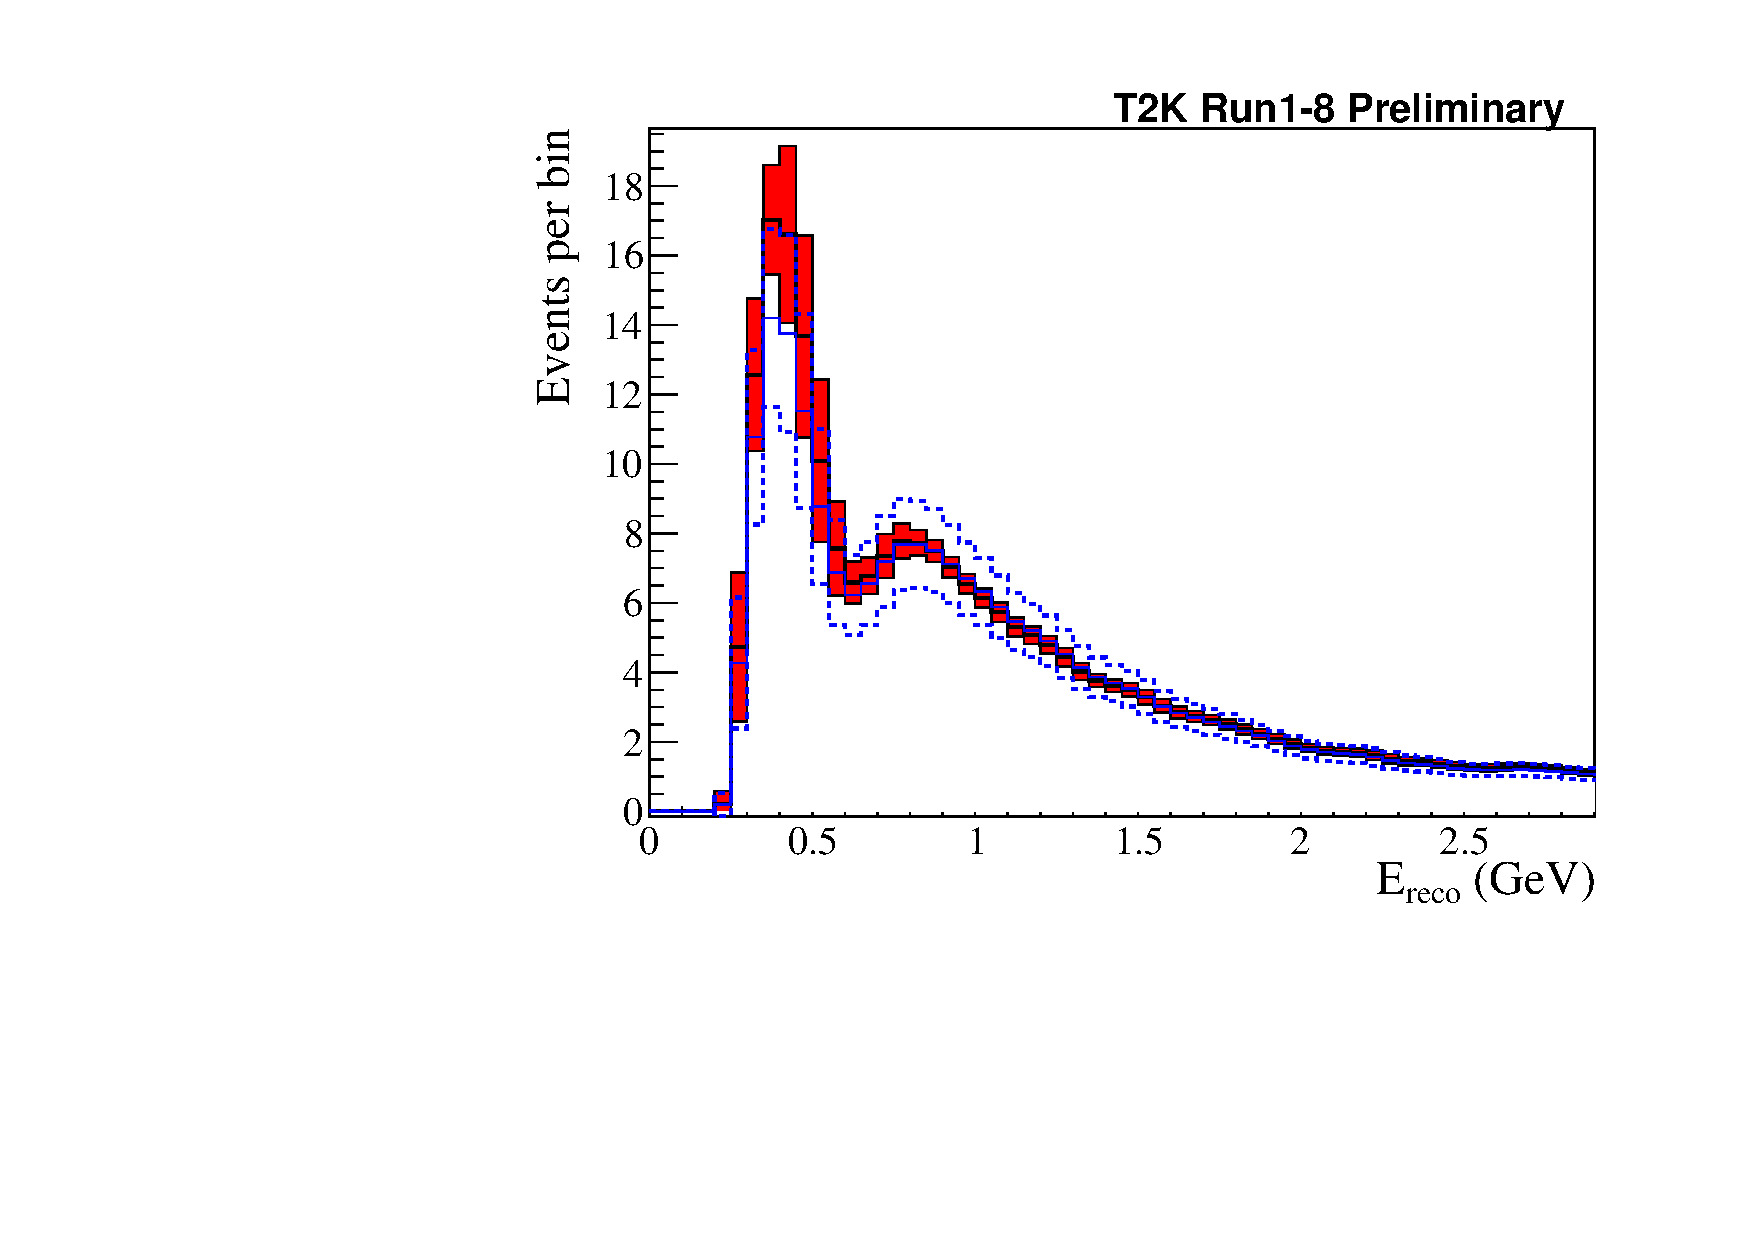
\includegraphics[width=0.9\textwidth]{images/systematics/envelopes/sk_error_table_1Rmu_all_envelope}
		\caption{Muon-like, neutrino mode}
	\end{subfigure}
	\begin{subfigure}[b]{0.49\textwidth}
		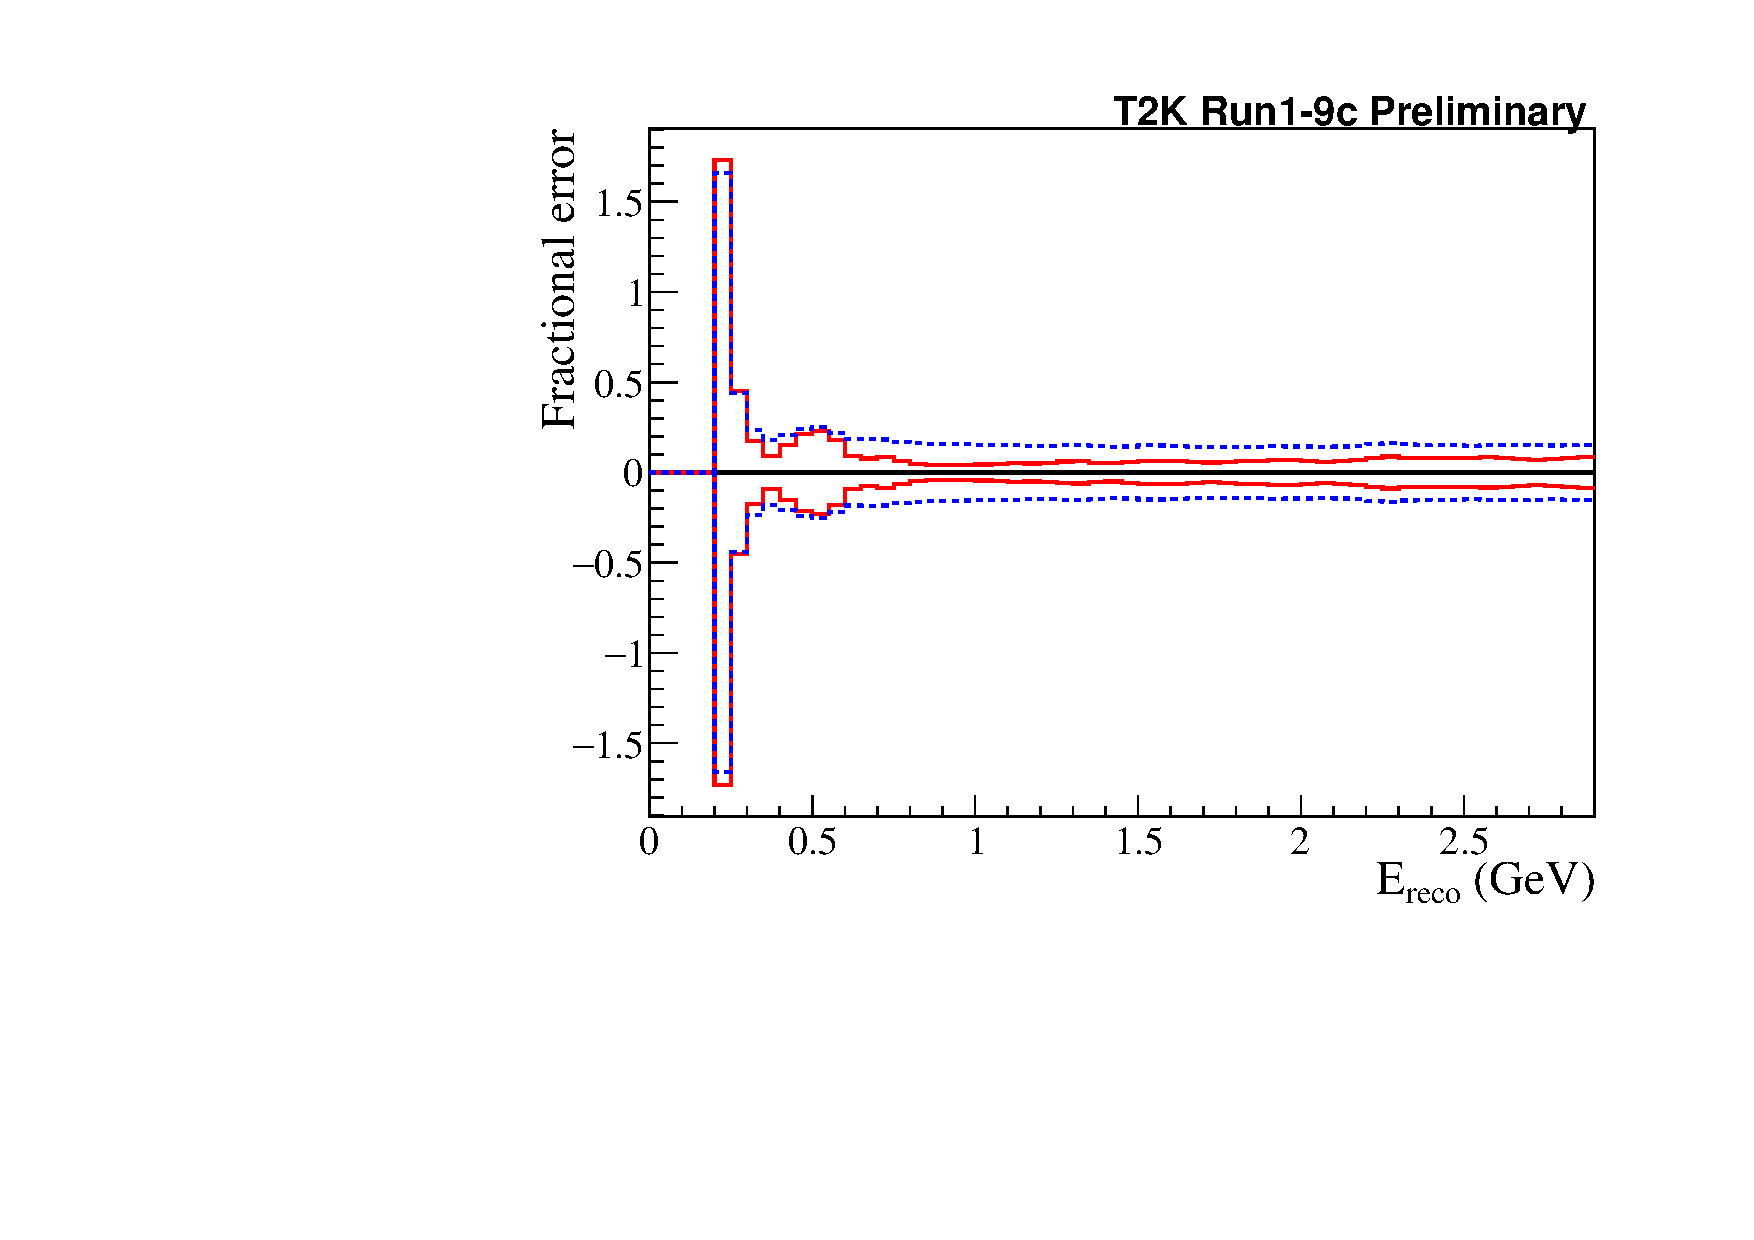
\includegraphics[width=0.9\textwidth]{images/systematics/envelopes/sk_error_table_1Rmu_all_envelope_fractional}
		\caption{Muon-like, neutrino mode}
	\end{subfigure}
	\begin{subfigure}[b]{0.49\textwidth}
		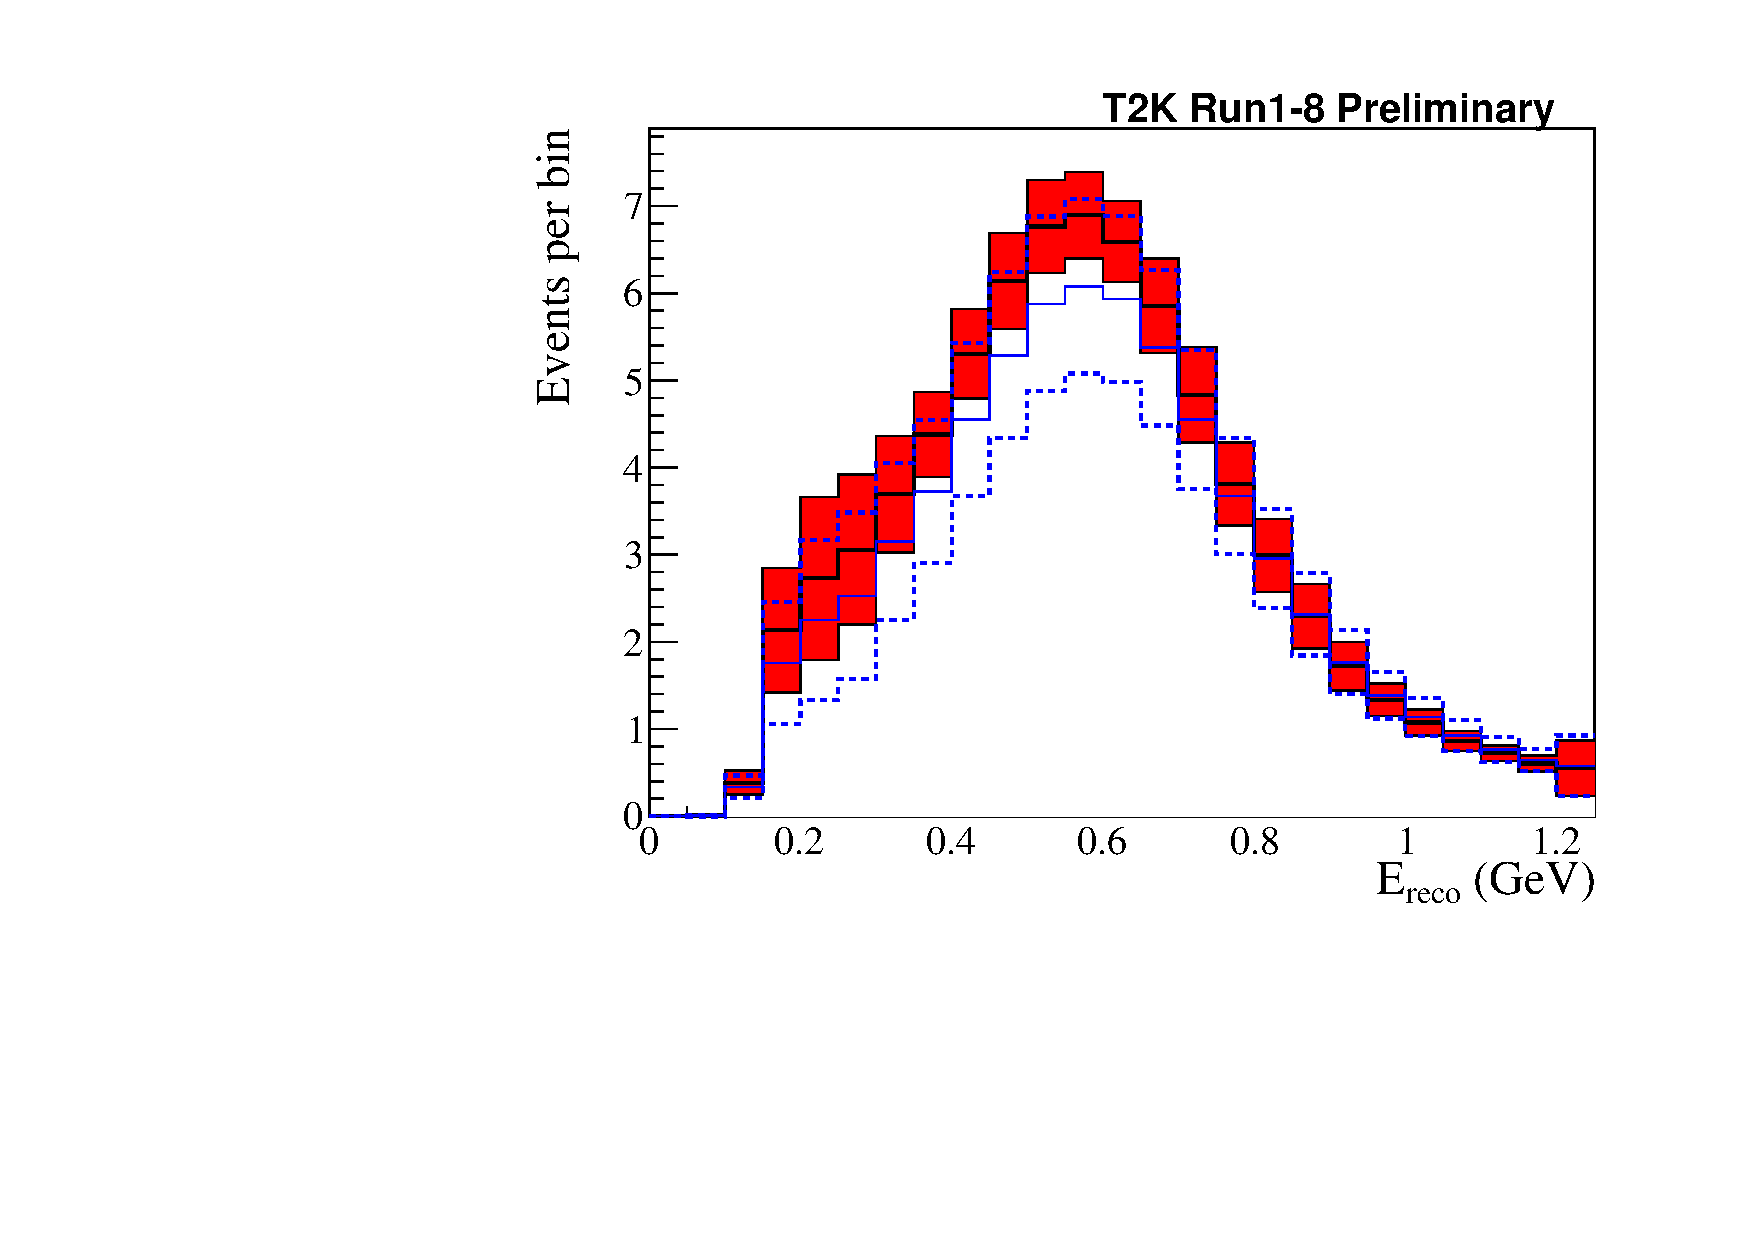
\includegraphics[width=0.9\textwidth]{images/systematics/envelopes/sk_error_table_1Re_all_envelope}
		\caption{Electron-like, neutrino mode}
	\end{subfigure}
	\begin{subfigure}[b]{0.49\textwidth}
		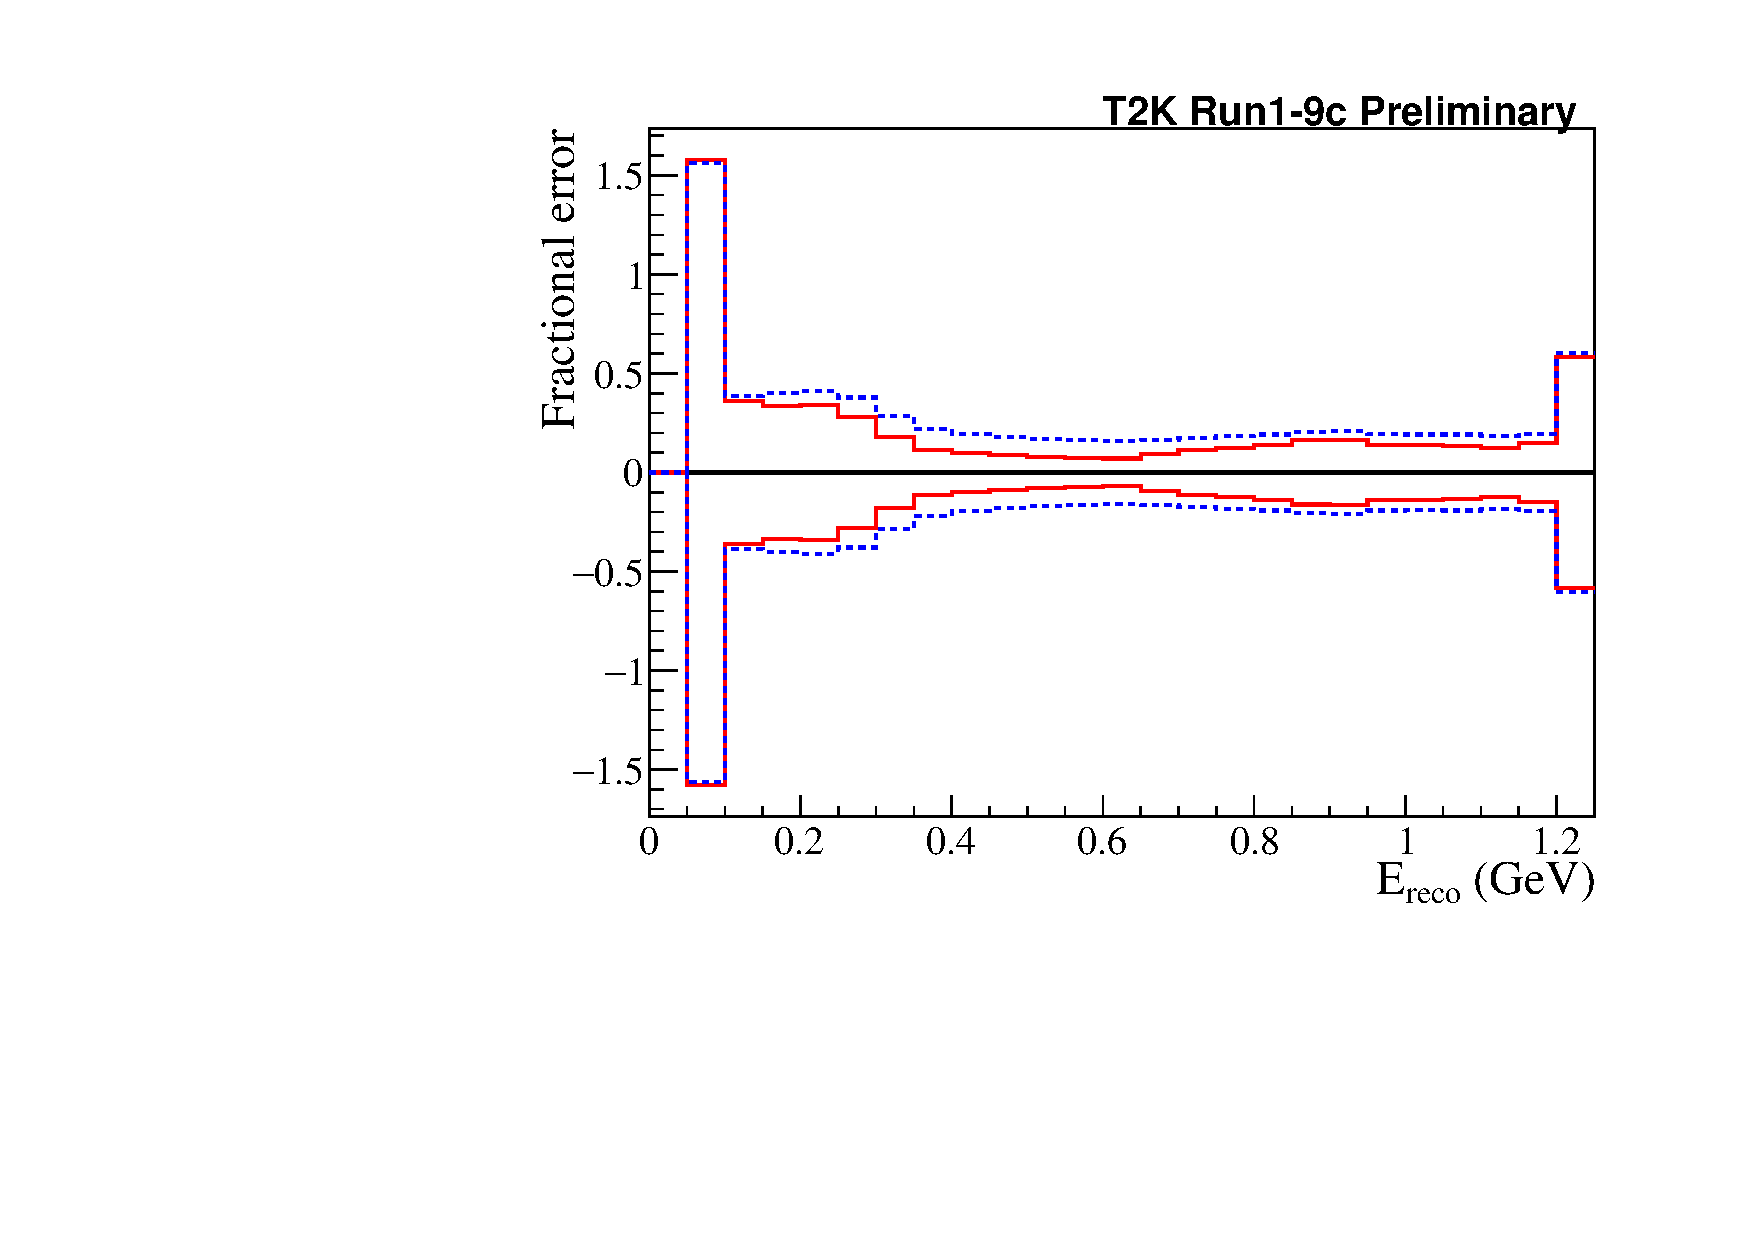
\includegraphics[width=0.9\textwidth]{images/systematics/envelopes/sk_error_table_1Re_all_envelope_fractional}
		\caption{Electron-like, neutrino mode}
	\end{subfigure}
	\begin{subfigure}[b]{0.49\textwidth}
		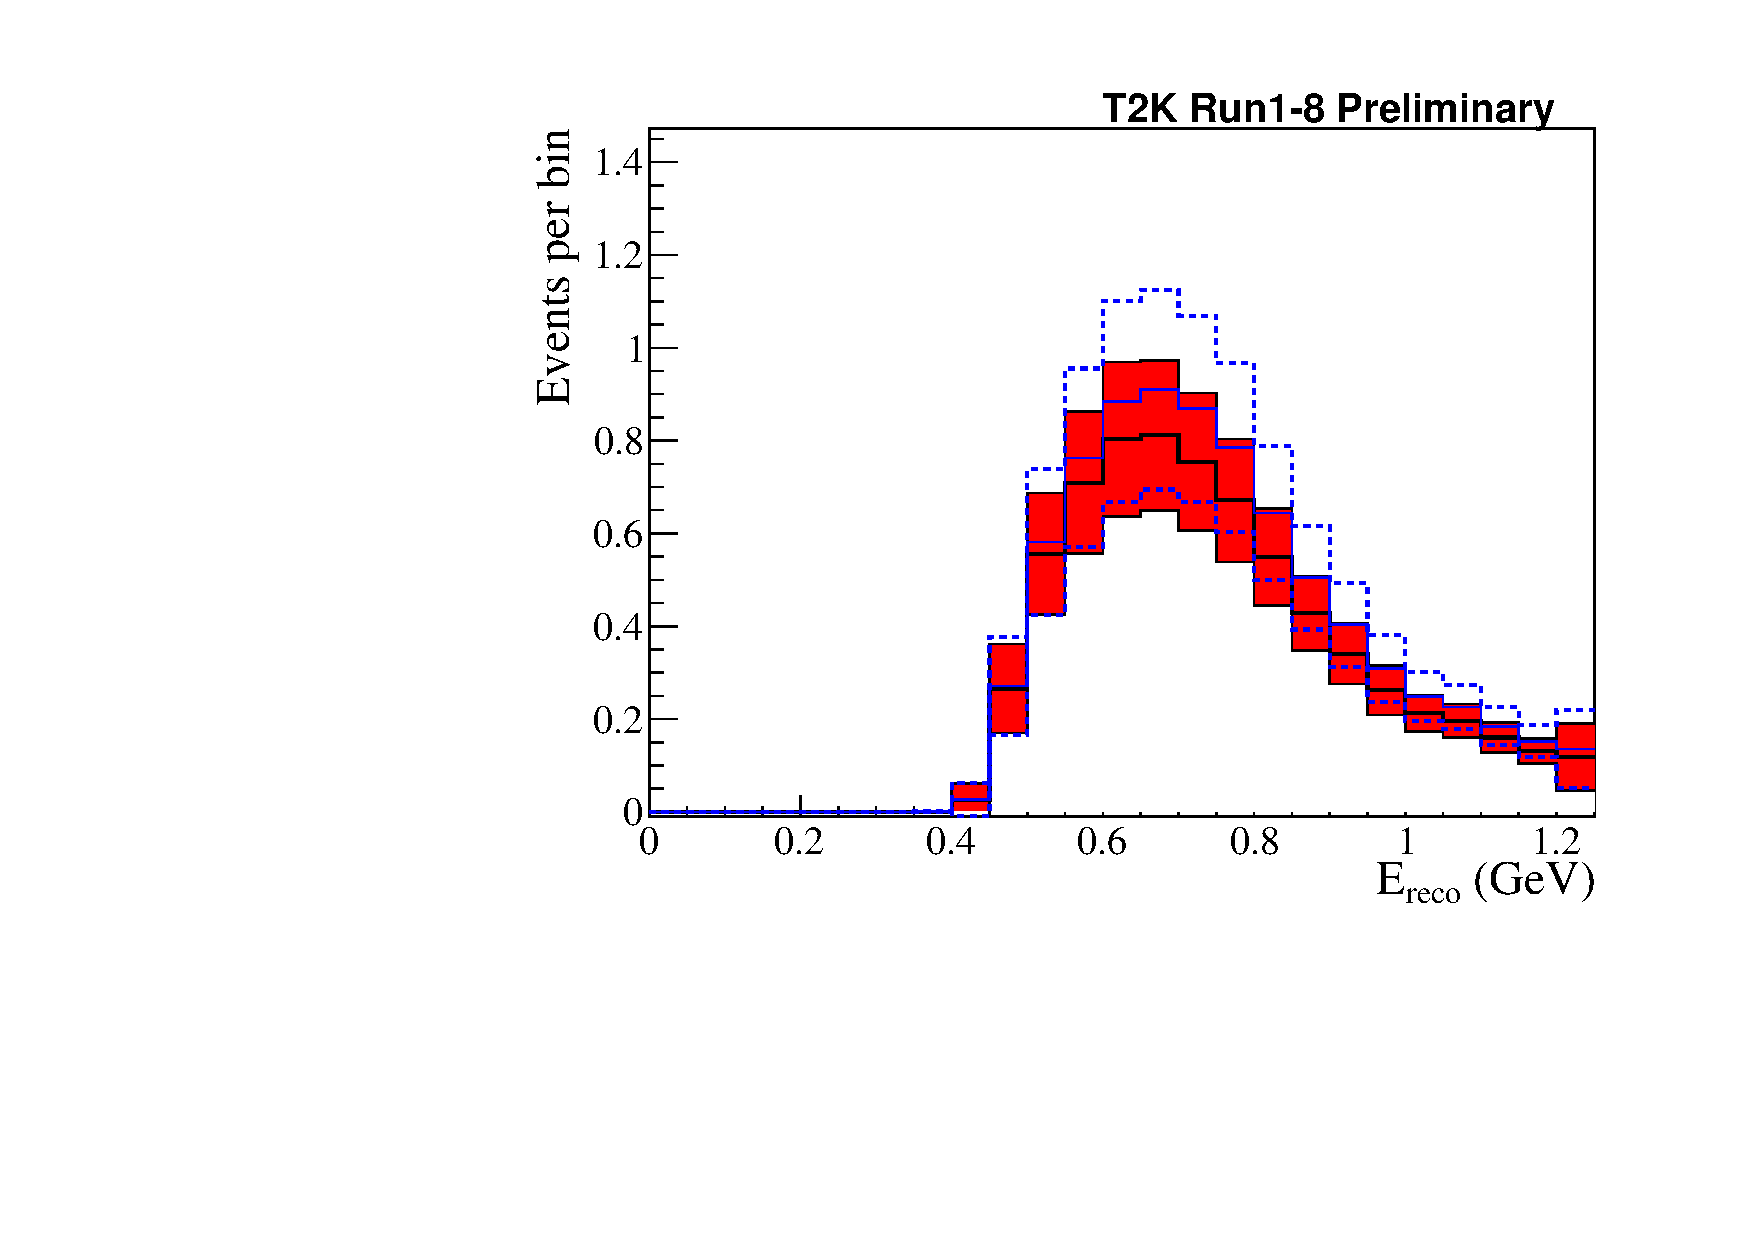
\includegraphics[width=0.9\textwidth]{images/systematics/envelopes/sk_error_table_MultiRe_all_envelope}
		\caption{\nueCConepi-like, neutrino mode}
	\end{subfigure}
	\begin{subfigure}[b]{0.49\textwidth}
		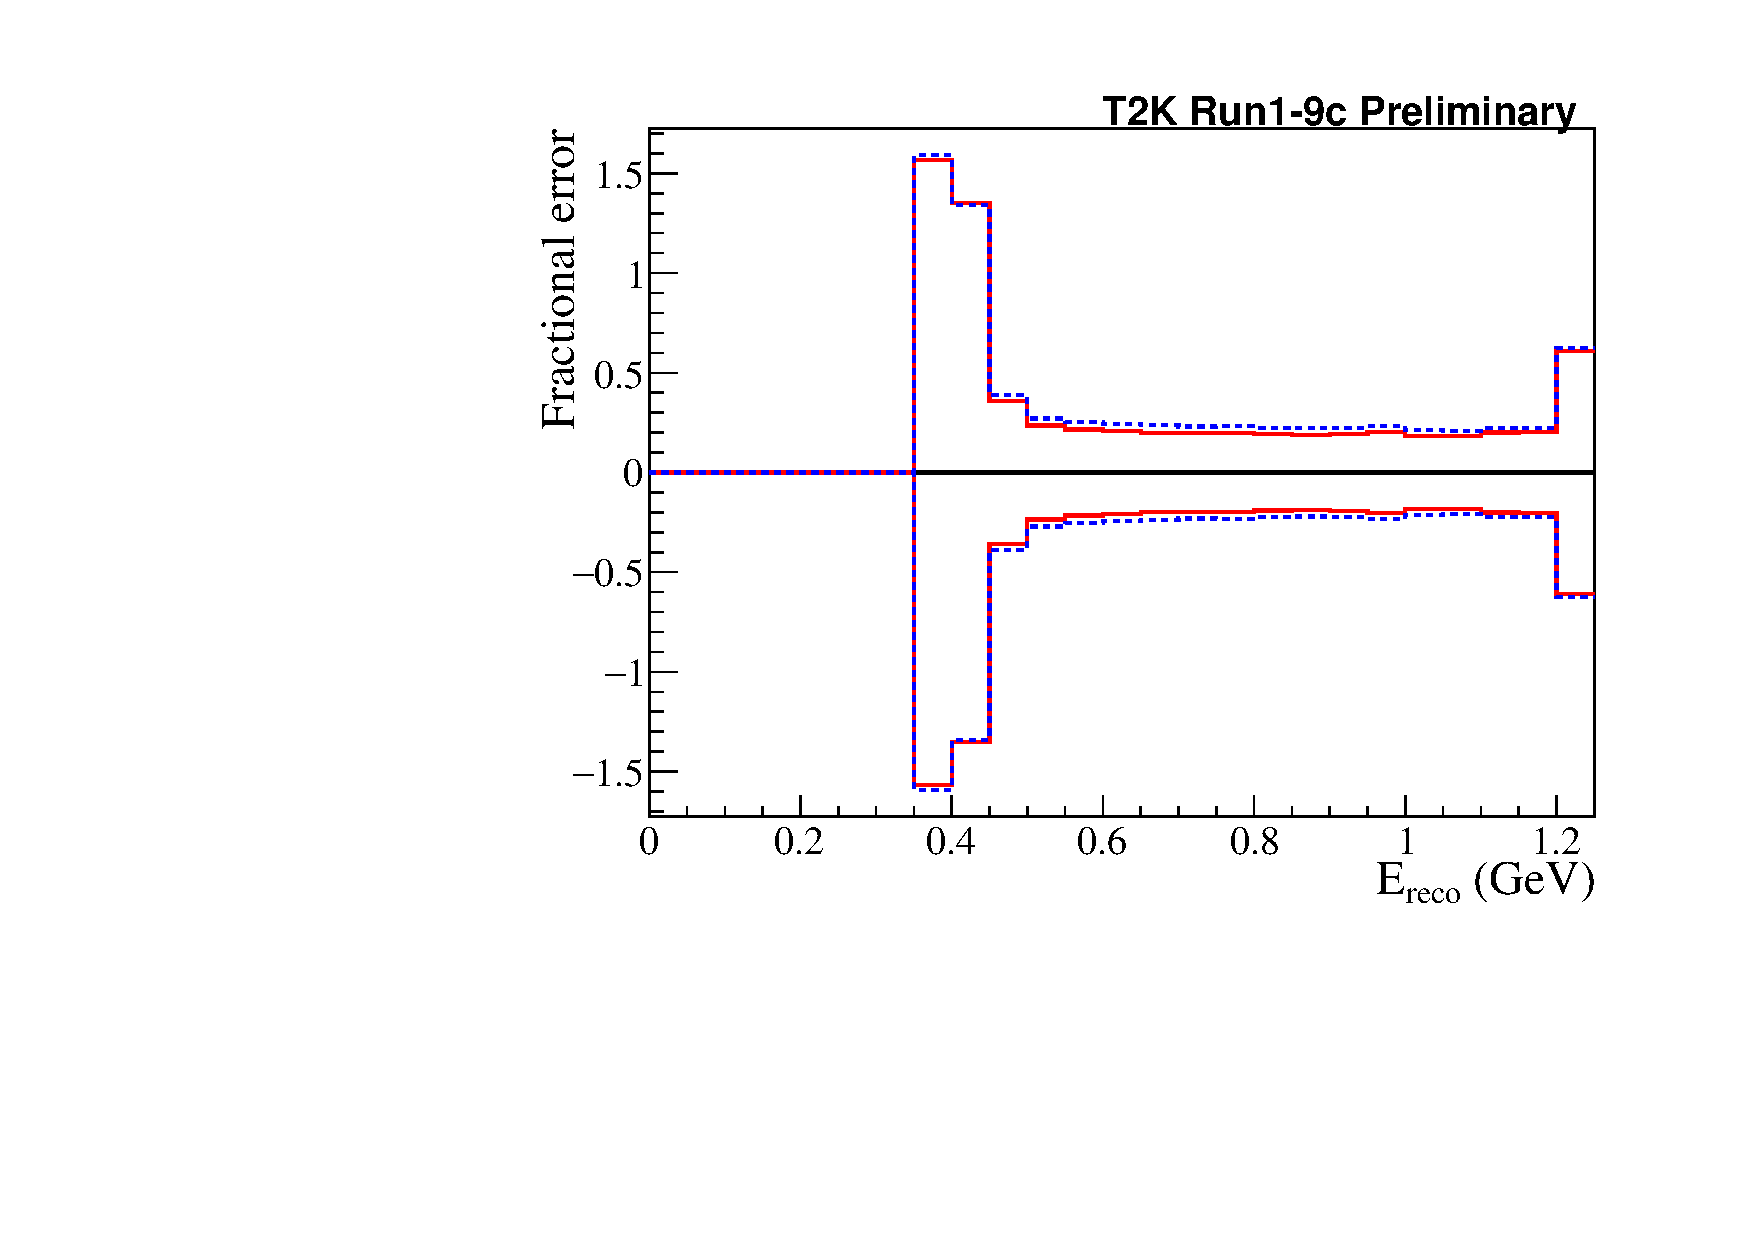
\includegraphics[width=0.9\textwidth]{images/systematics/envelopes/sk_error_table_MultiRe_all_envelope_fractional}
		\caption{\nueCConepi-like, neutrino mode}
	\end{subfigure}
	\caption {
		Error envelopes (left) and fractional errors (right) for the reconstructed neutrino energy spectrum for all systematic parameters for pre-BANFF (blue) and post-BANFF (red) errors. \NumToysSmall toys are generated for the Asimov data set A with randomized systematic parameters with correlations taken into account. Since \deltacp, \ssqthtwothree, \dmsqtwothree and the mass hierarchy will be measured, only the uncertainty on \ssqthonethree, \ssqthonetwo and \dmsqonetwo are taken into account.
	}
	\label{fig:sk_envelopes_all}
\end{figure*}
\clearpage
\begin{figure*}
	\center
	\begin{subfigure}[b]{0.49\textwidth}
		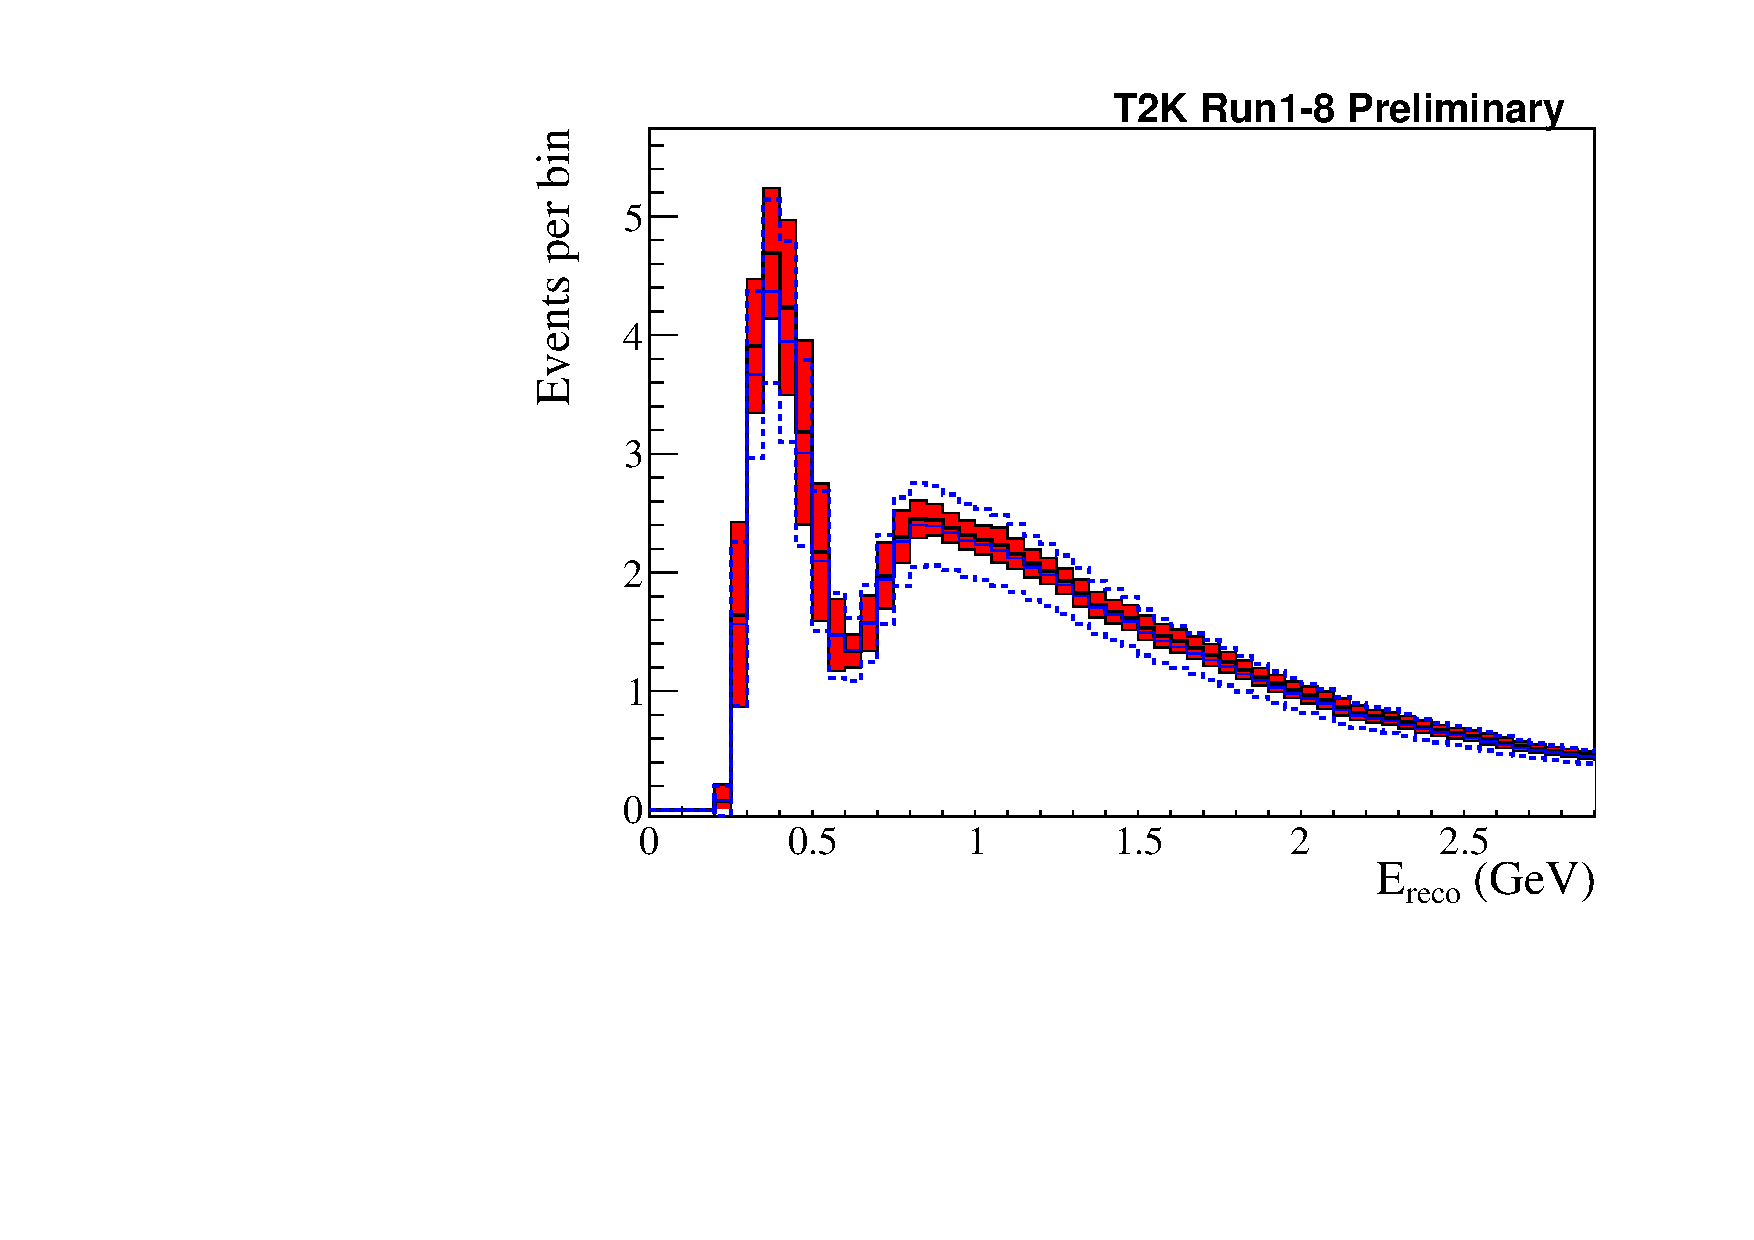
\includegraphics[width=0.9\textwidth]{images/systematics/envelopes/sk_error_table_RHC1Rmu_all_envelope}
		\caption{Muon-like, antineutrino mode}
	\end{subfigure}
	\begin{subfigure}[b]{0.49\textwidth}
		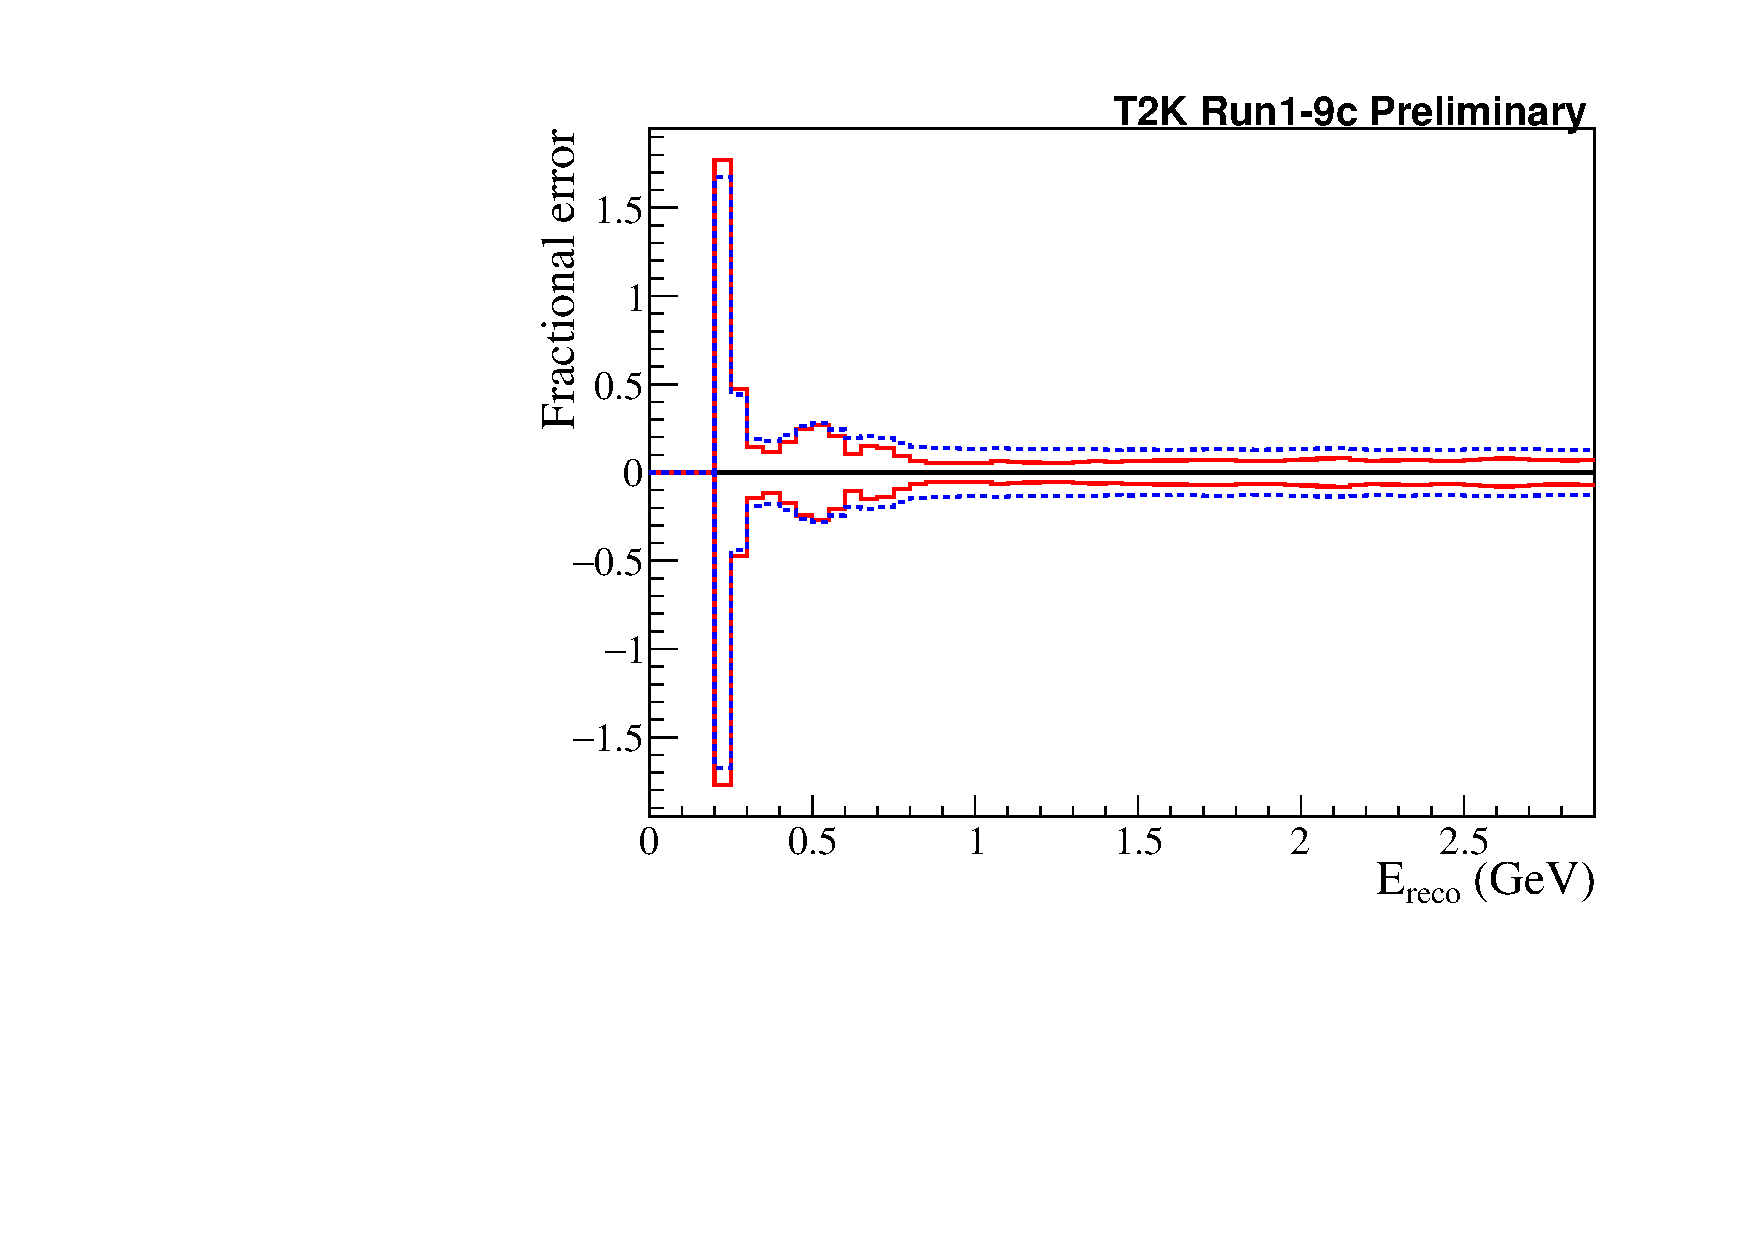
\includegraphics[width=0.9\textwidth]{images/systematics/envelopes/sk_error_table_RHC1Rmu_all_envelope_fractional}
		\caption{Muon-like, antineutrino mode}
	\end{subfigure}
	\begin{subfigure}[b]{0.49\textwidth}
		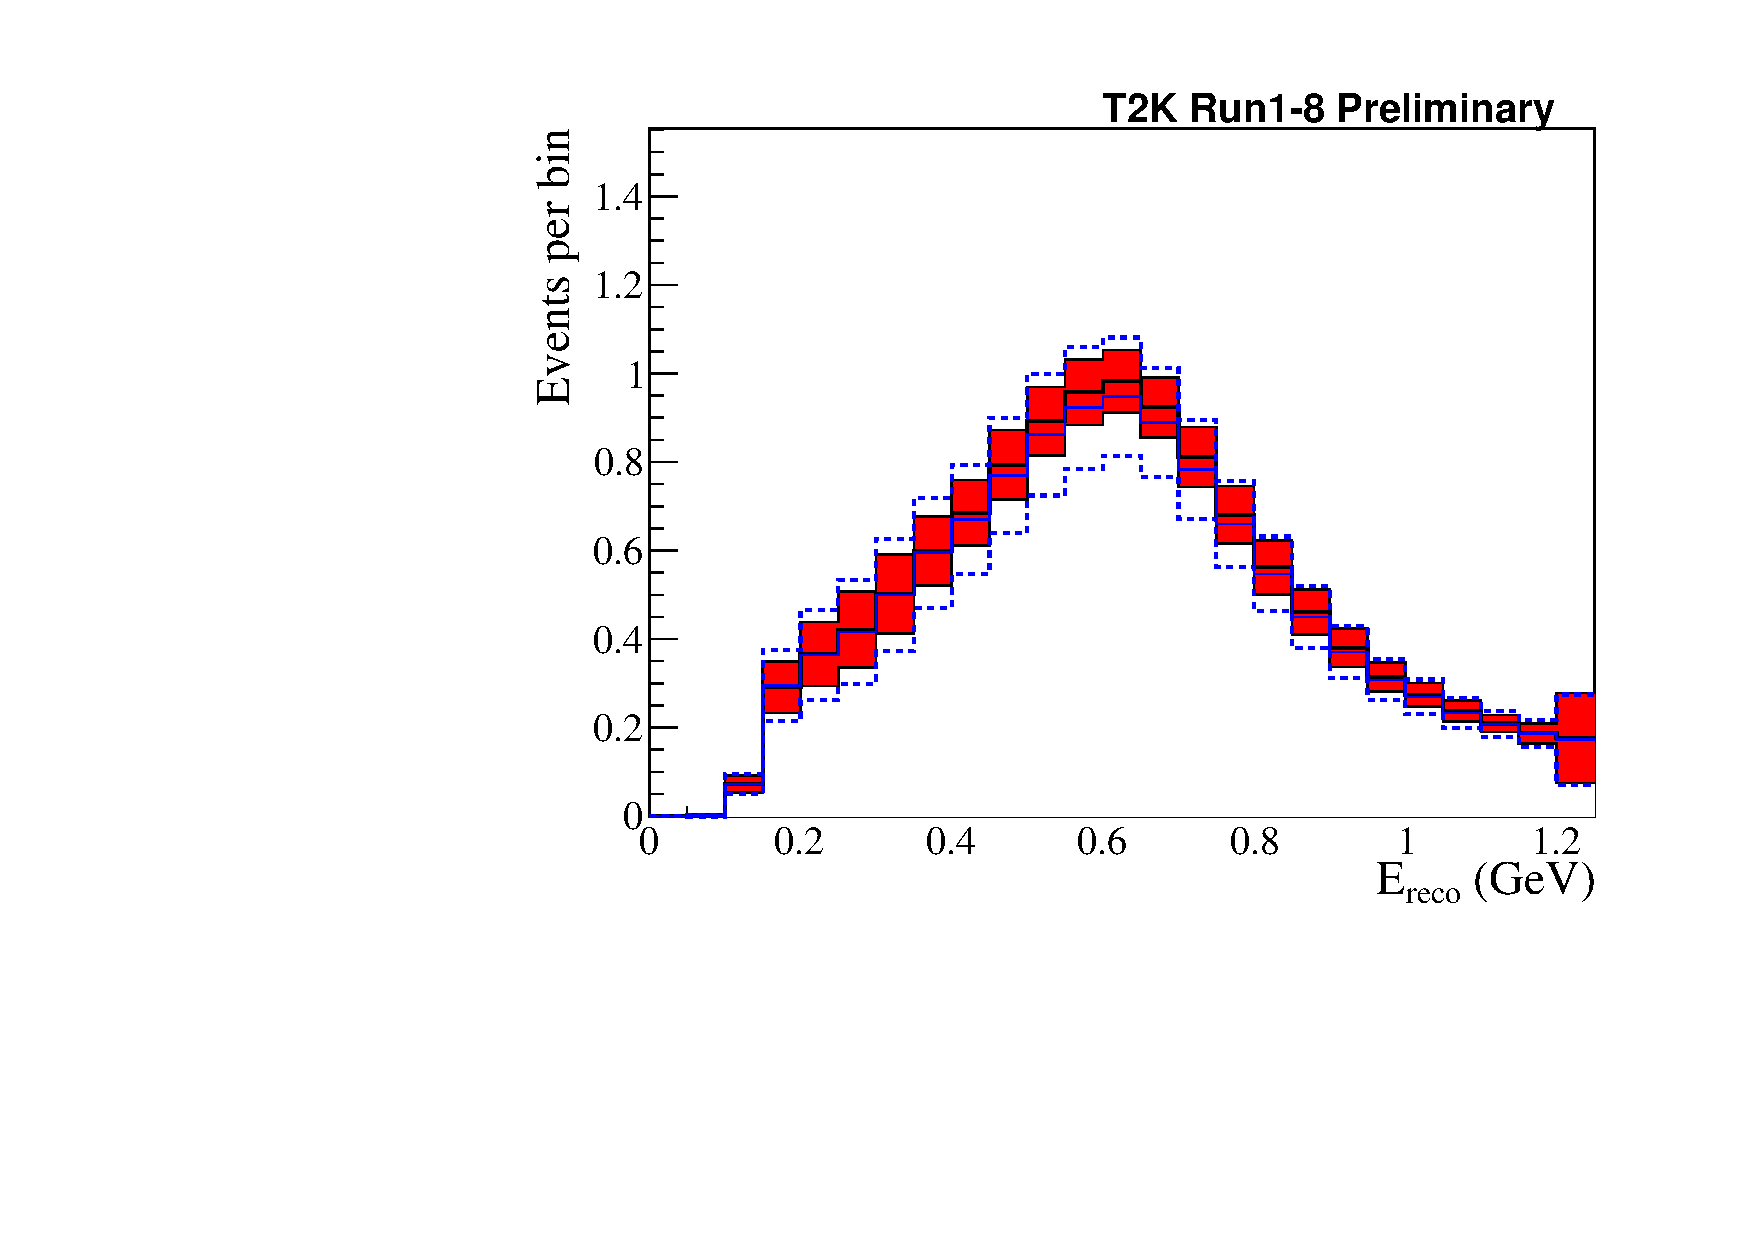
\includegraphics[width=0.9\textwidth]{images/systematics/envelopes/sk_error_table_RHC1Re_all_envelope}
		\caption{Electron-like antineutrino mode}
	\end{subfigure}
	\begin{subfigure}[b]{0.49\textwidth}
		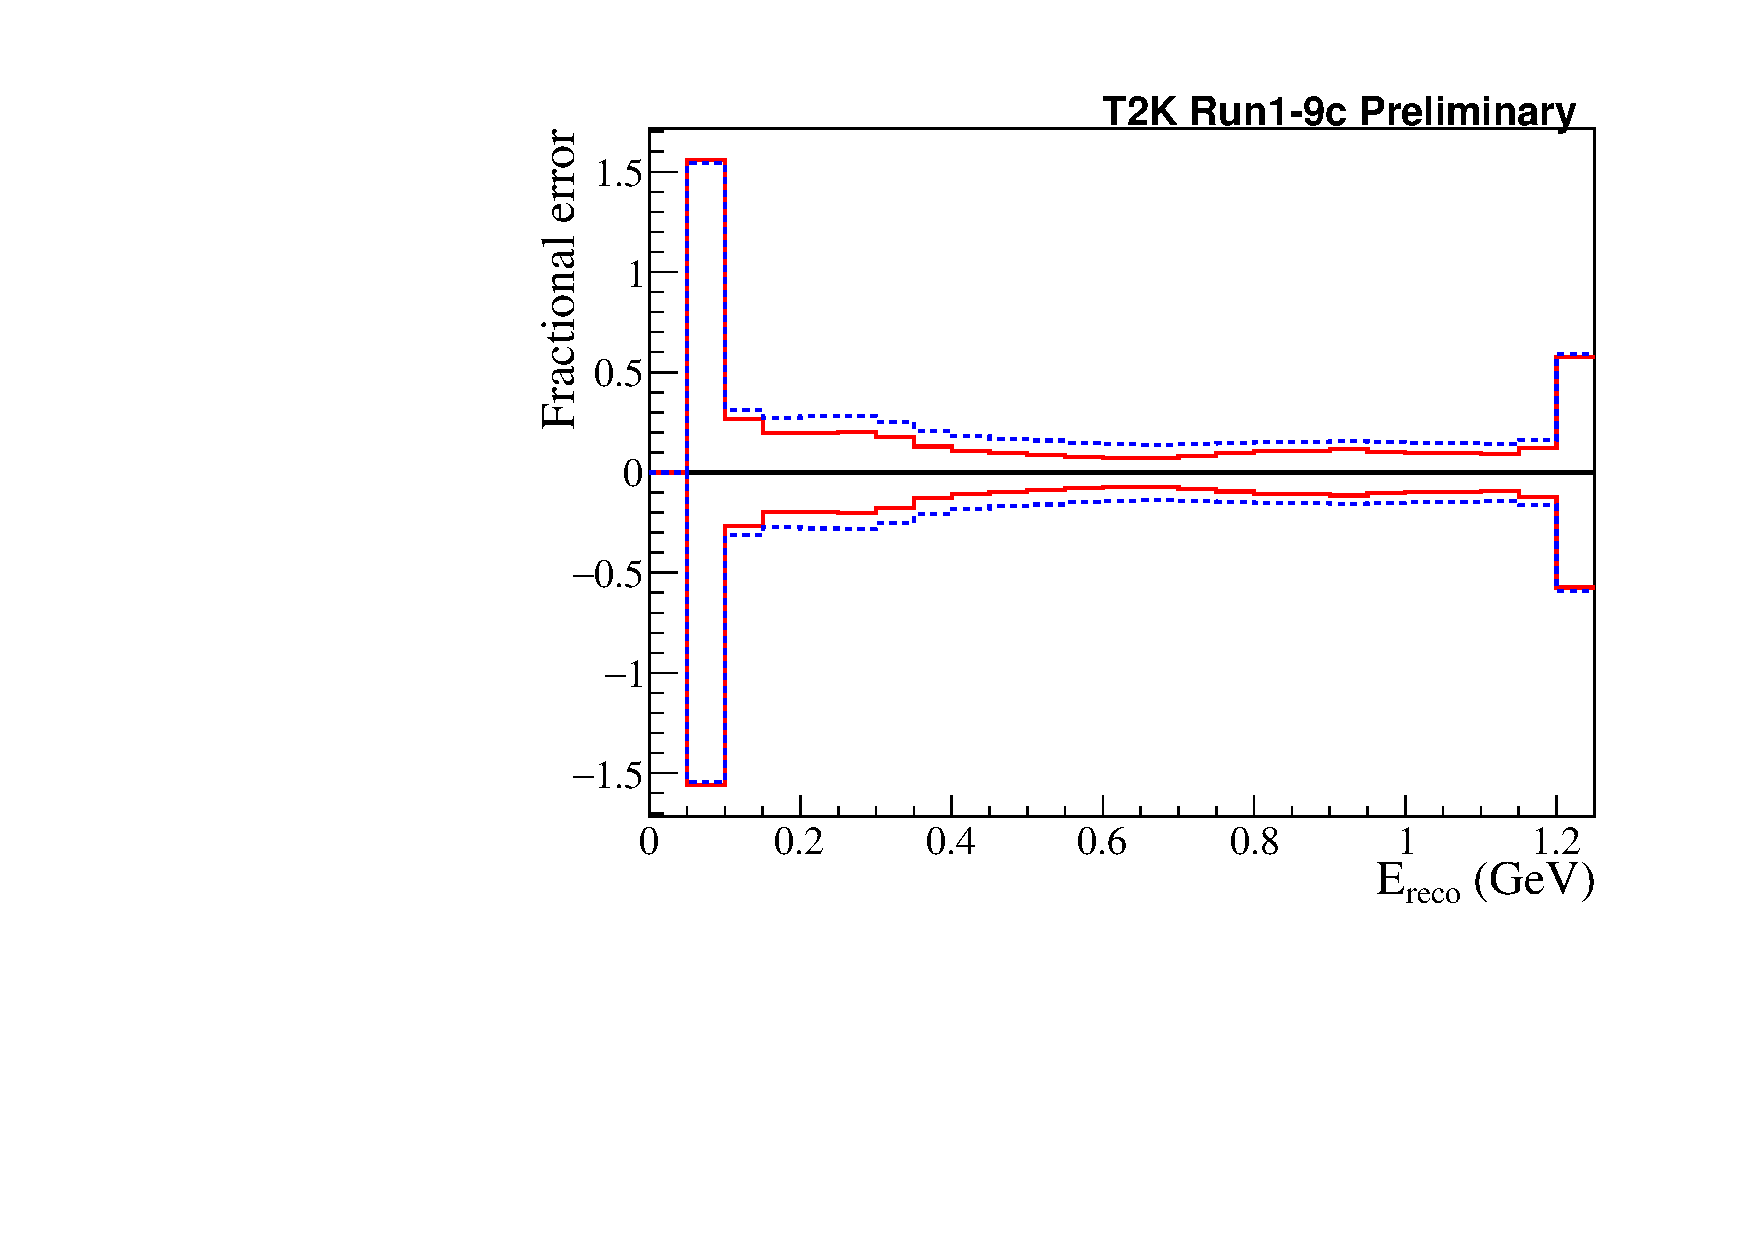
\includegraphics[width=0.9\textwidth]{images/systematics/envelopes/sk_error_table_RHC1Re_all_envelope_fractional}
		\caption{Electron-like antineutrino mode}
	\end{subfigure}
	\caption {
		Error envelopes (left) and fractional errors (right) for the reconstructed neutrino energy spectrum for all systematic parameters for pre-BANFF (blue) and post-BANFF (red) errors. \NumToysSmall toys are generated for the Asimov data set A with randomized systematic parameters with correlations taken into account. Since \deltacp, \ssqthtwothree, \dmsqtwothree and the mass hierarchy will be measured, only the uncertainty on \ssqthonethree, \ssqthonetwo and \dmsqonetwo are taken into account.
	}
	\label{fig:sk_envelopes_all_b}
\end{figure*}
\clearpage
\begin{figure*}
	\center
	\begin{subfigure}[b]{0.49\textwidth}
		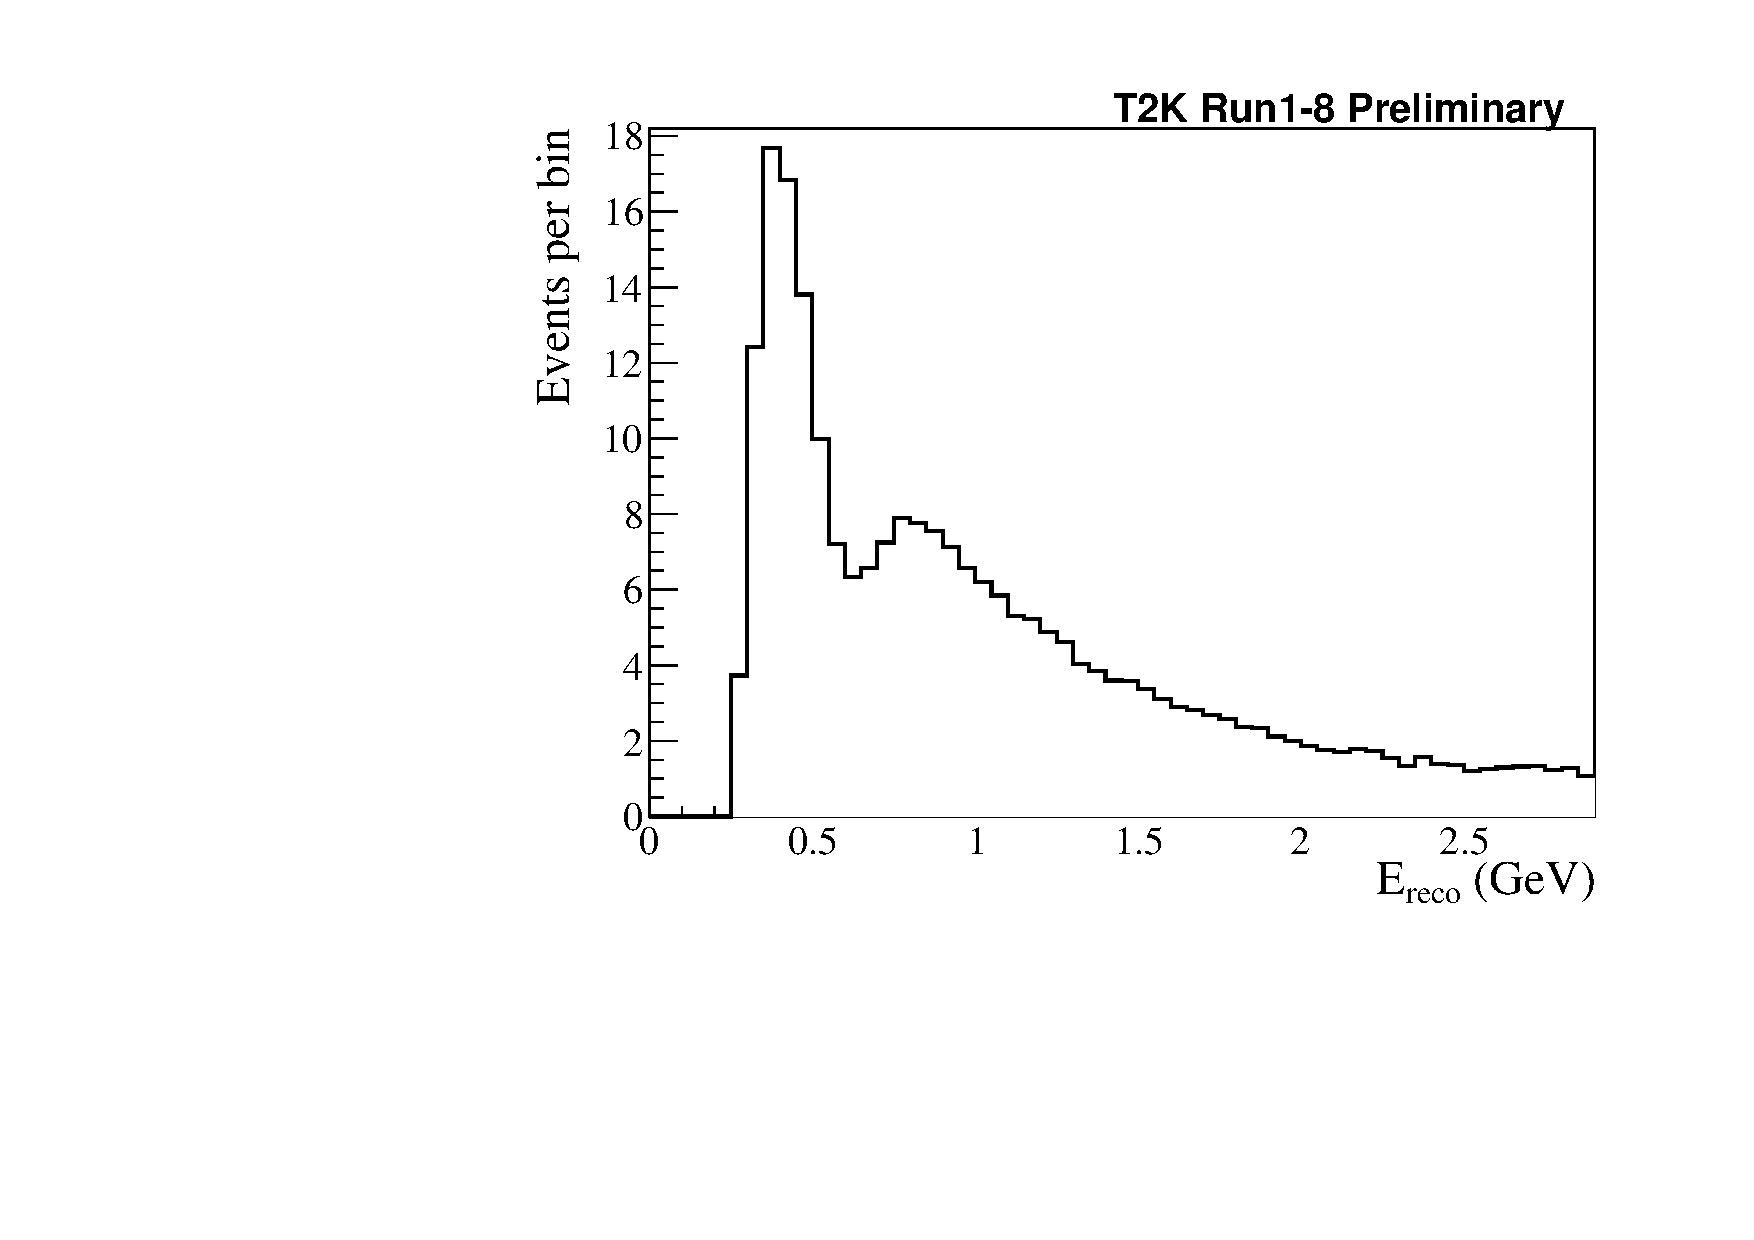
\includegraphics[width=0.9\textwidth]{images/systematics/envelopes/sk_error_table_1Rmu_osc_envelope}
		\caption{Muon-like, neutrino mode}
	\end{subfigure}
	\begin{subfigure}[b]{0.49\textwidth}
		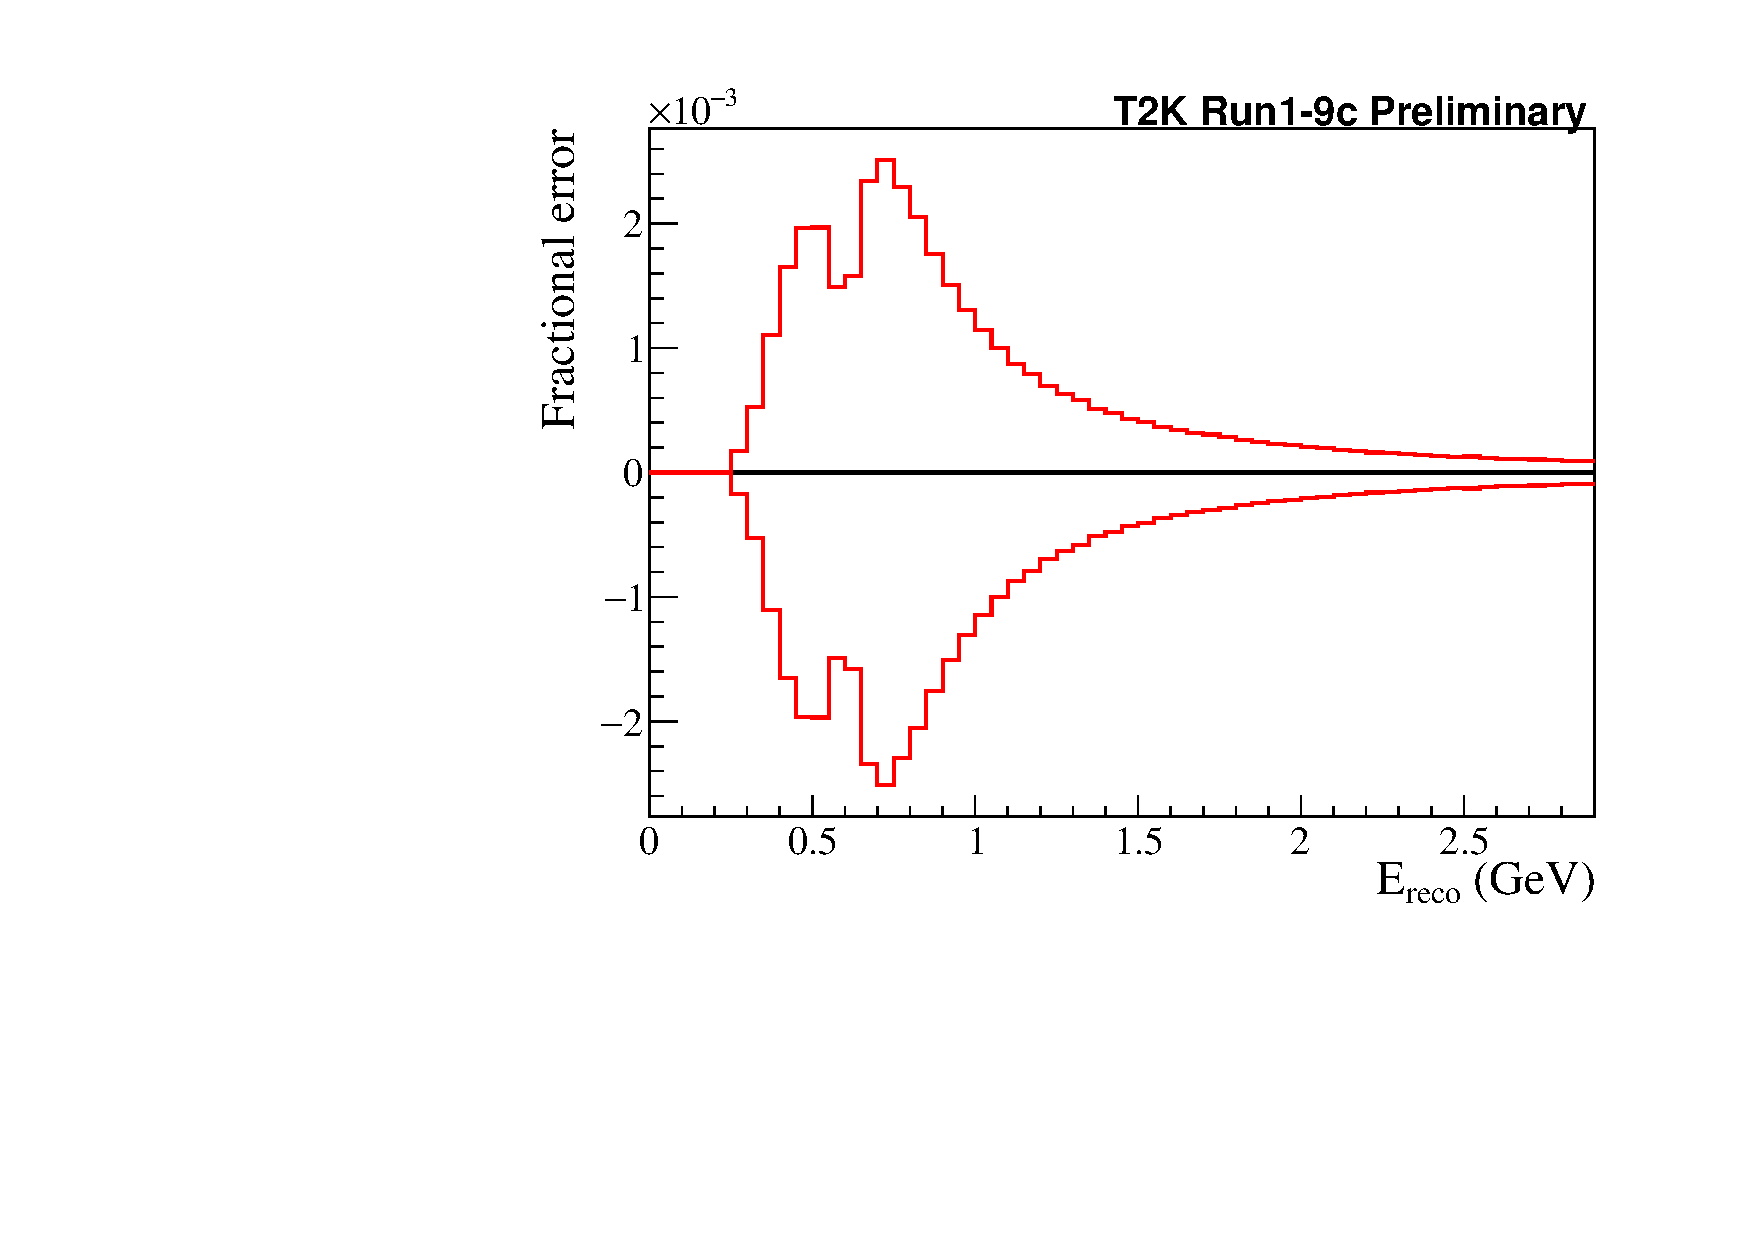
\includegraphics[width=0.9\textwidth]{images/systematics/envelopes/sk_error_table_1Rmu_osc_envelope_fractional}
		\caption{Muon-like, neutrino mode}
	\end{subfigure}
	\begin{subfigure}[b]{0.49\textwidth}
		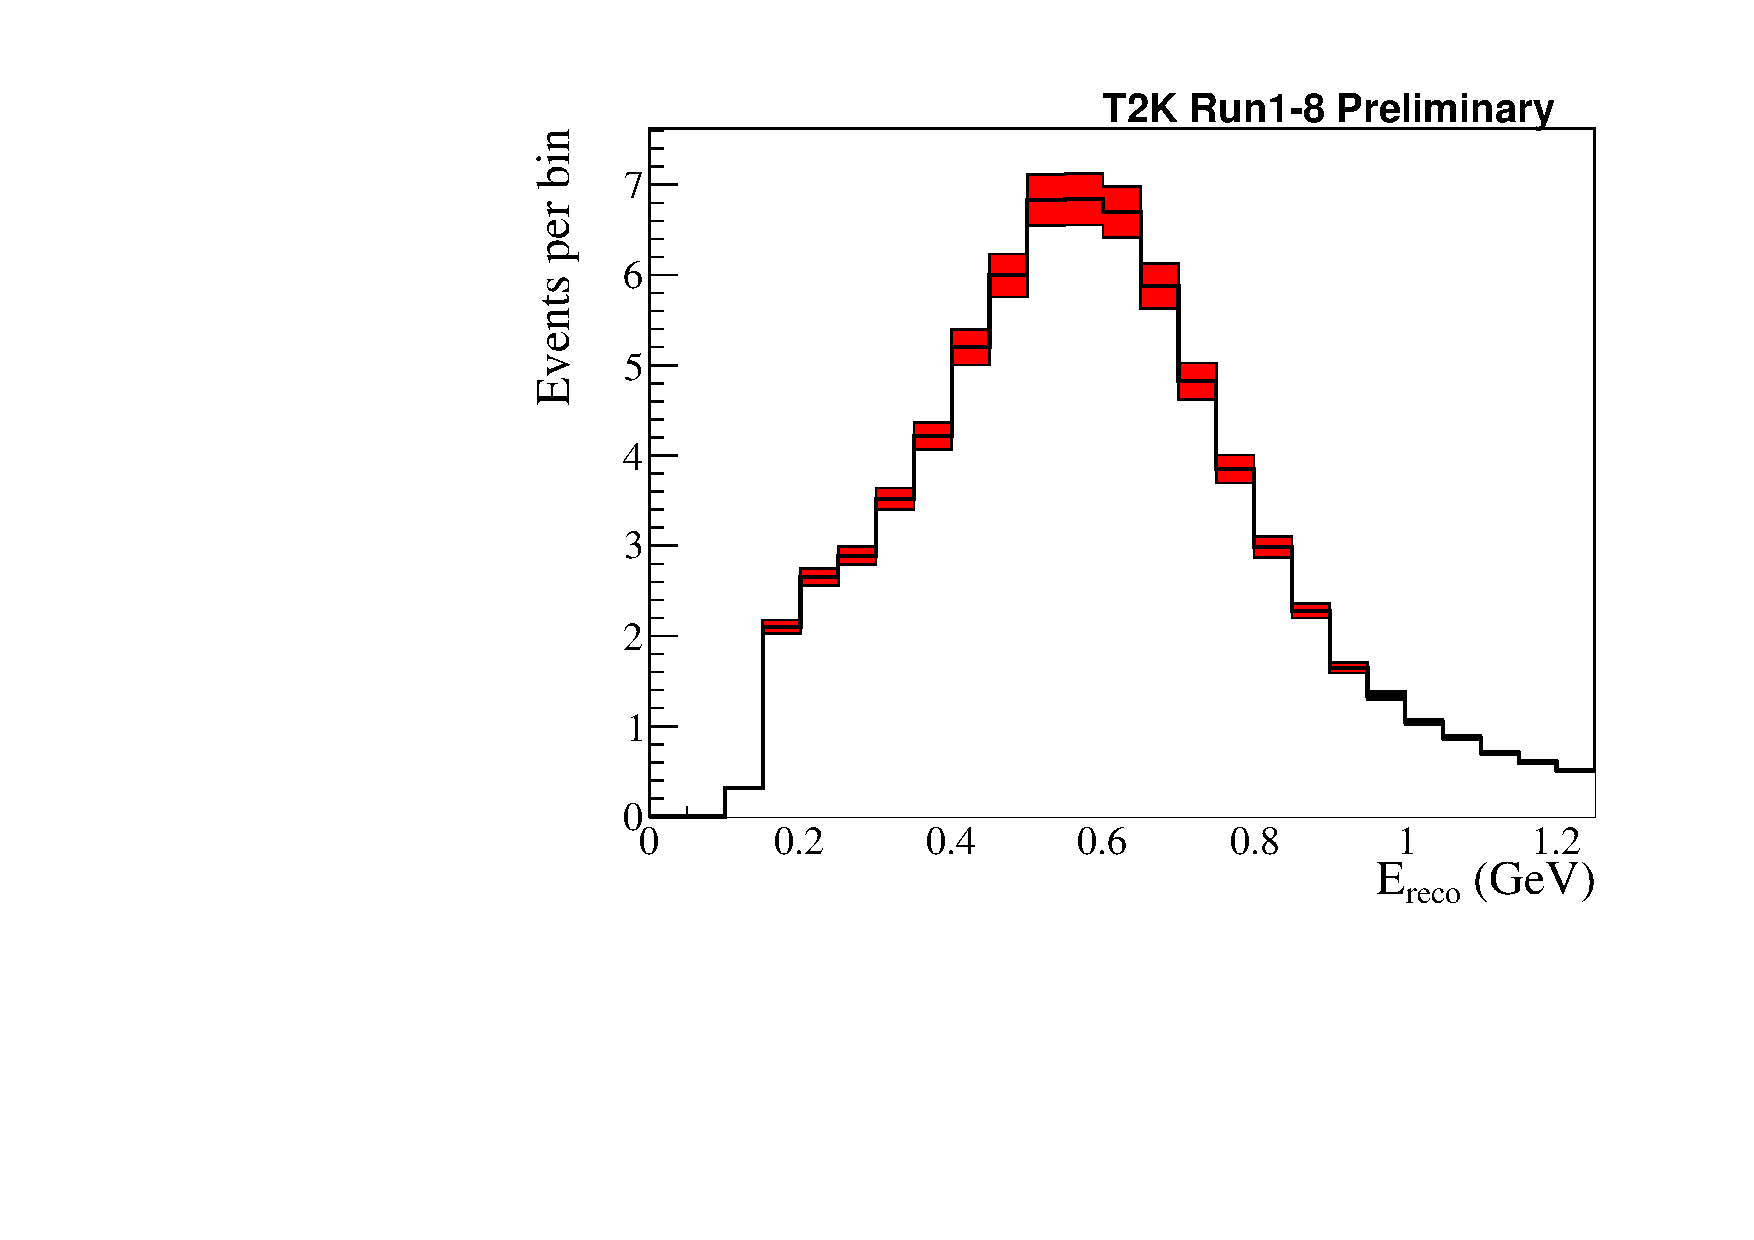
\includegraphics[width=0.9\textwidth]{images/systematics/envelopes/sk_error_table_1Re_osc_envelope}
		\caption{Electron-like, neutrino mode}
	\end{subfigure}
	\begin{subfigure}[b]{0.49\textwidth}
		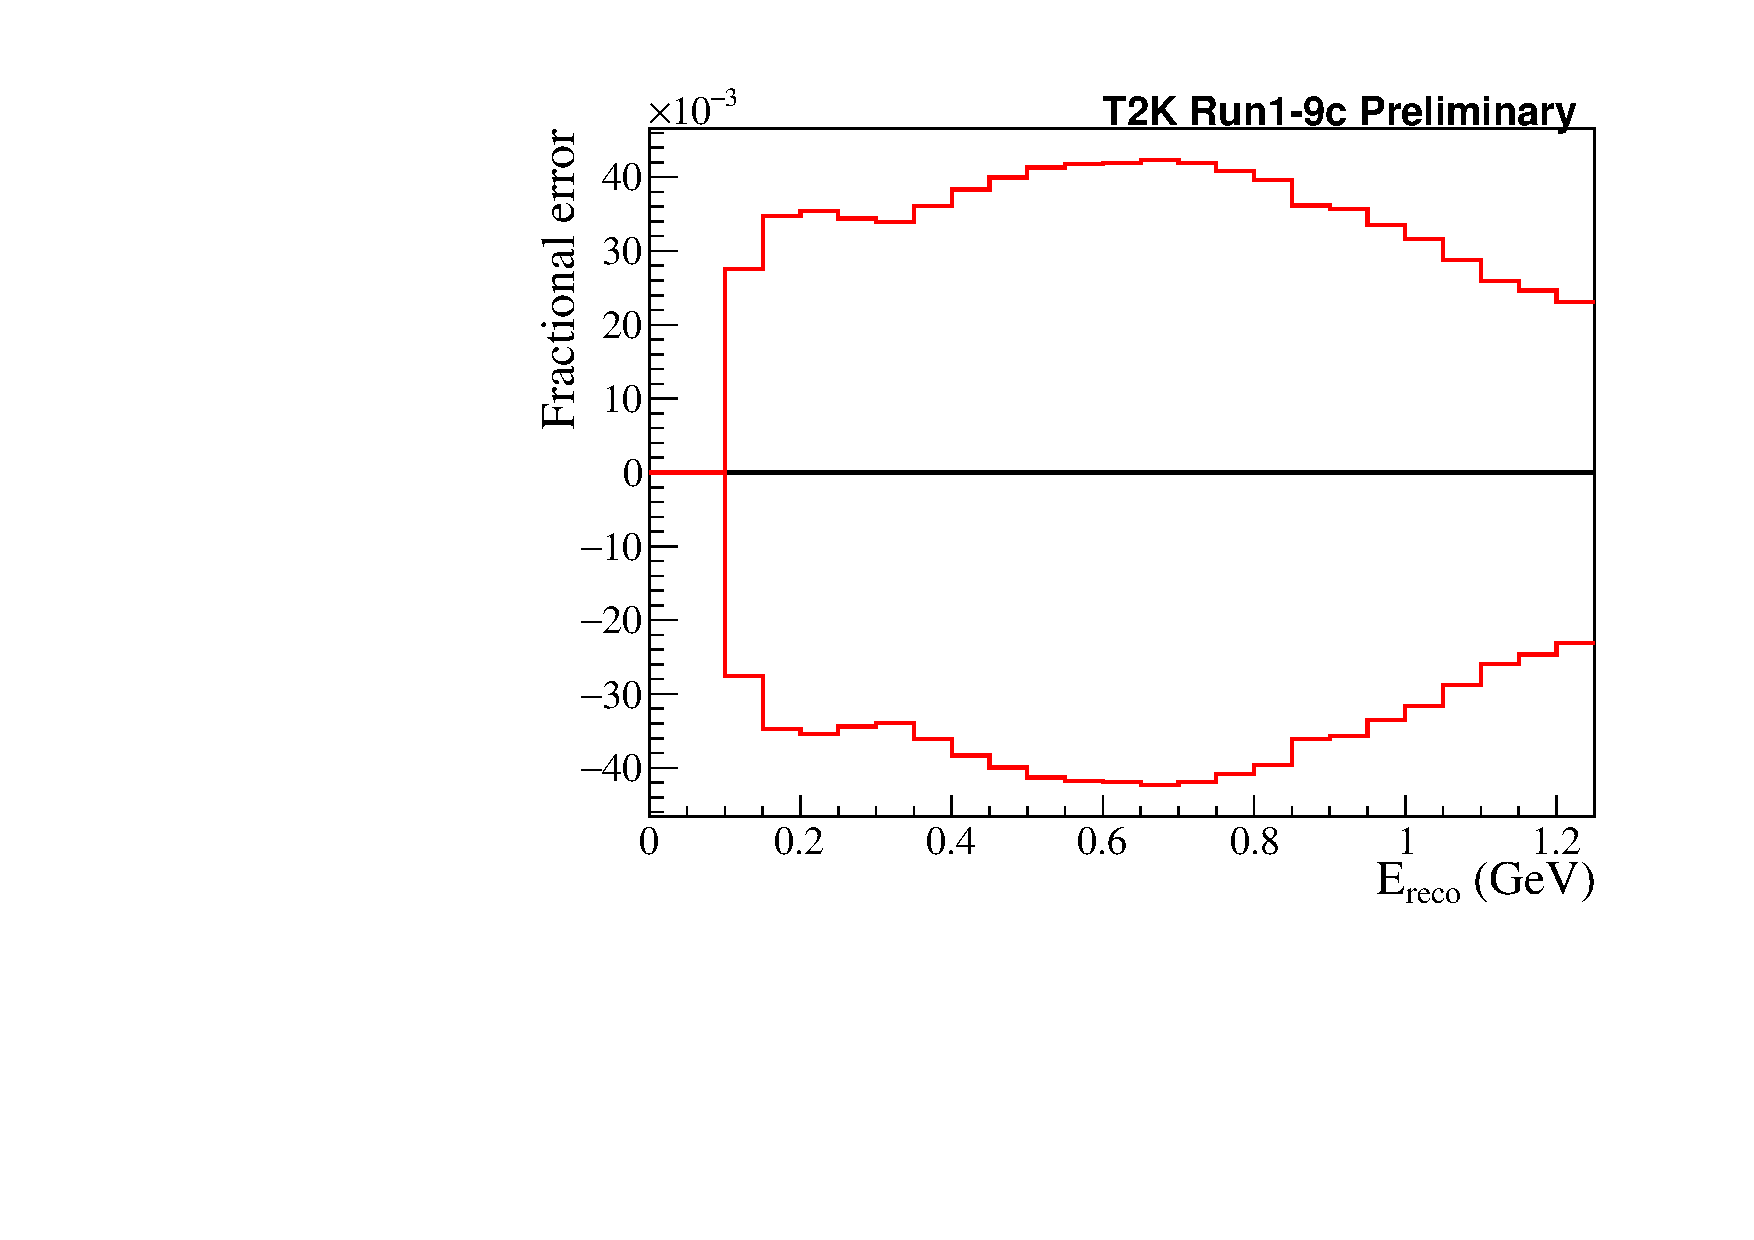
\includegraphics[width=0.9\textwidth]{images/systematics/envelopes/sk_error_table_1Re_osc_envelope_fractional}
		\caption{Electron-like, neutrino mode}
	\end{subfigure}
	\begin{subfigure}[b]{0.49\textwidth}
		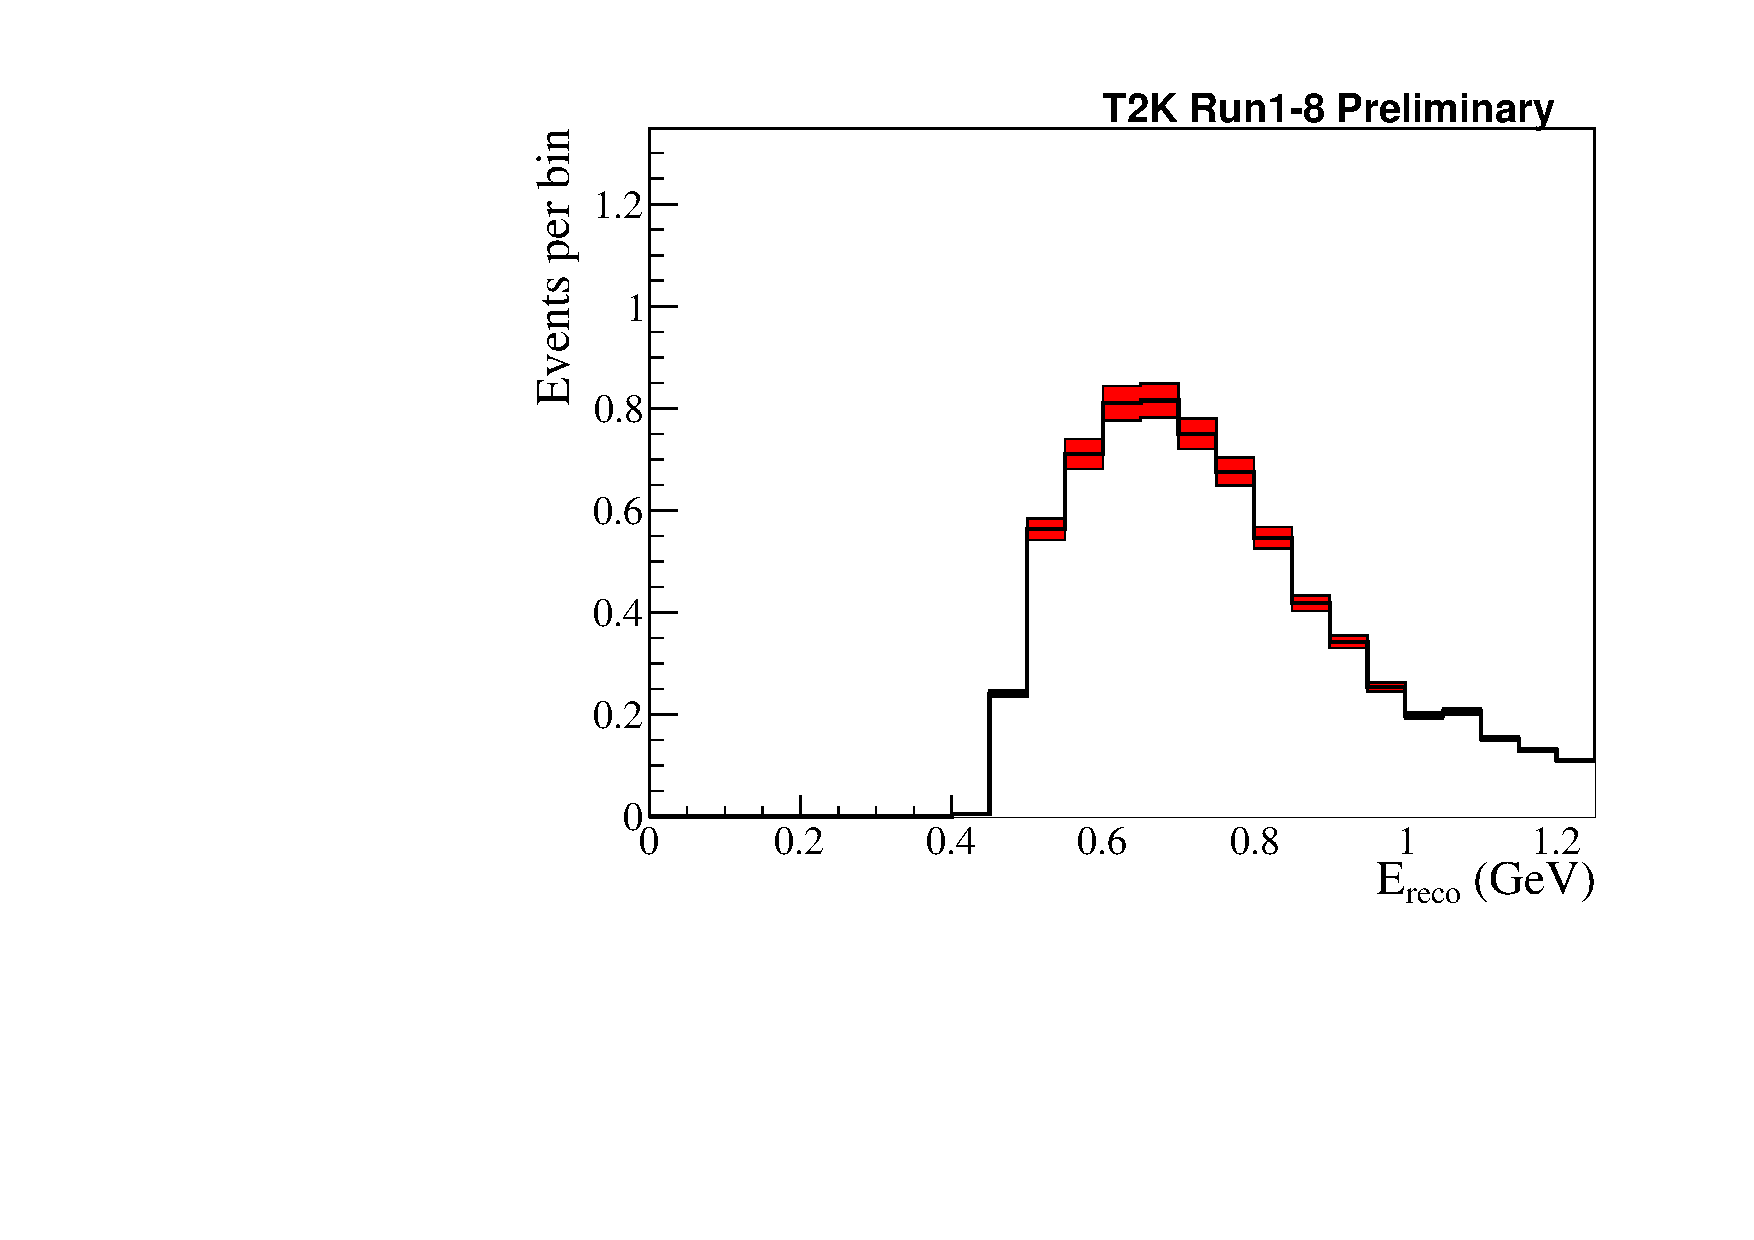
\includegraphics[width=0.9\textwidth]{images/systematics/envelopes/sk_error_table_MultiRe_osc_envelope}
		\caption{\nueCConepi-like, neutrino mode}
	\end{subfigure}
	\begin{subfigure}[b]{0.49\textwidth}
		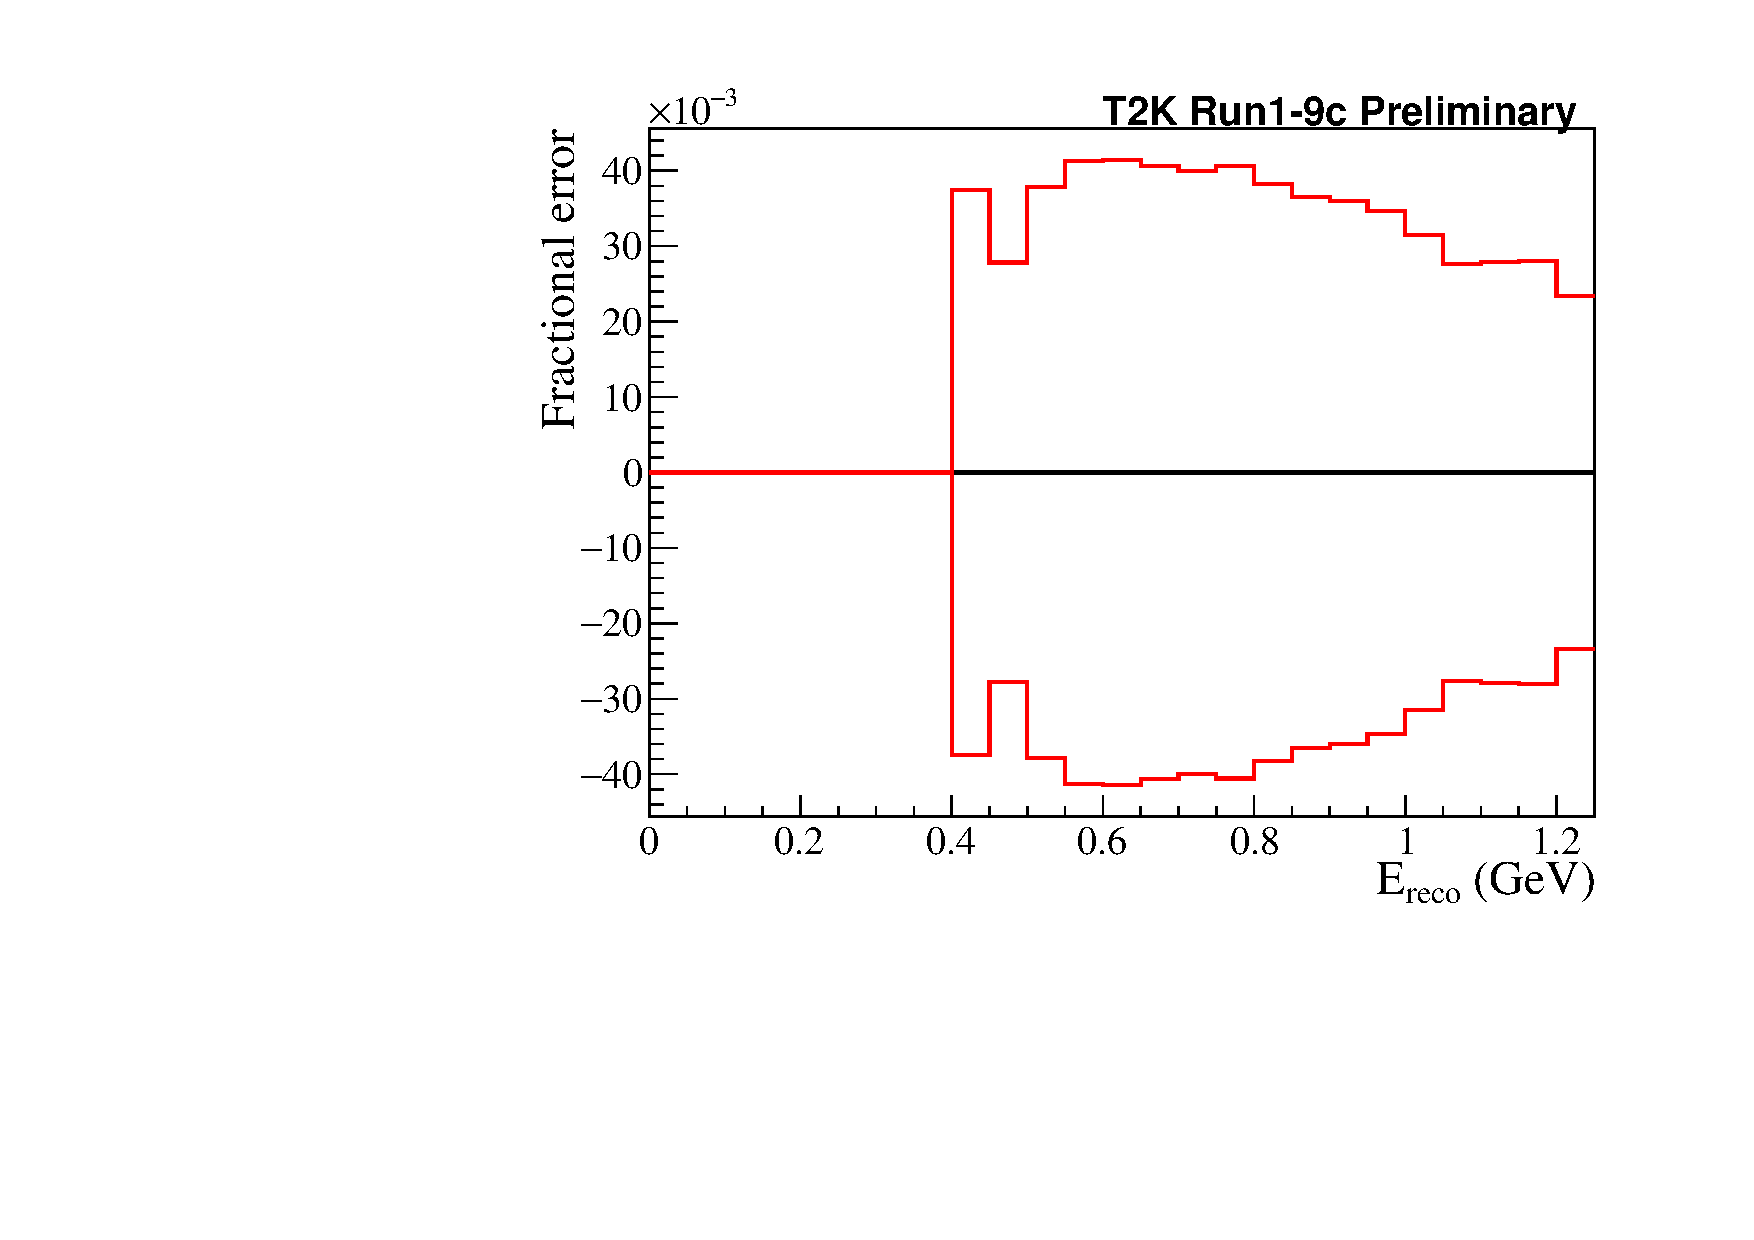
\includegraphics[width=0.9\textwidth]{images/systematics/envelopes/sk_error_table_MultiRe_osc_envelope_fractional}
		\caption{\nueCConepi-like, neutrino mode}
	\end{subfigure}
	\caption {
		Error envelopes (left) and fractional errors (right) for the reconstructed neutrino energy spectrum for all oscillation nuisance parameters. \NumToysSmall toys are generated for the Asimov data set A with randomized systematic parameters with correlations taken into account. Since \deltacp, \ssqthtwothree, \dmsqtwothree and the mass hierarchy will be measured, only the uncertainty on \ssqthonethree, \ssqthonetwo and \dmsqonetwo are taken into account.
	}
	\label{fig:sk_envelopes_osc}
\end{figure*}
\clearpage

\begin{figure*}
	\center
	\begin{subfigure}[b]{0.49\textwidth}
		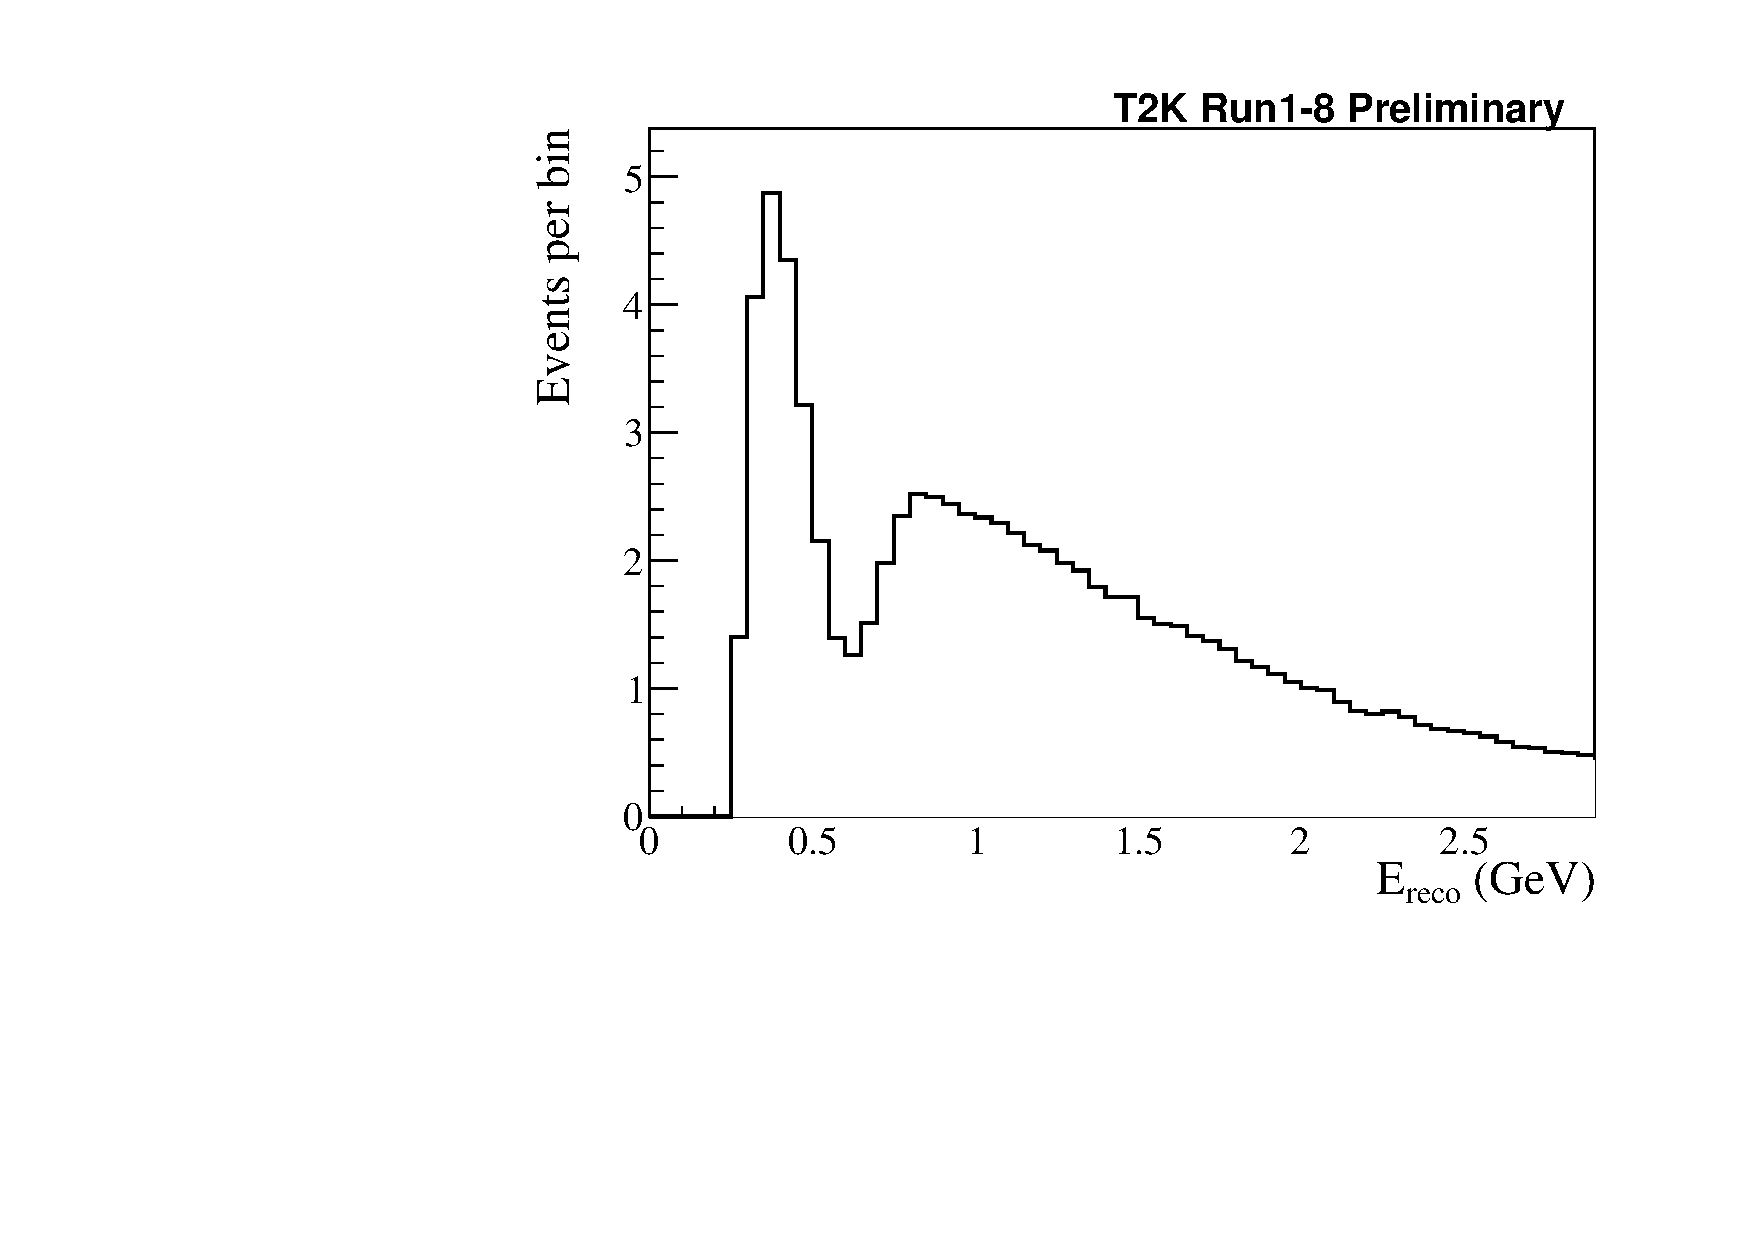
\includegraphics[width=0.9\textwidth]{images/systematics/envelopes/sk_error_table_RHC1Rmu_osc_envelope}
		\caption{Muon-like, antineutrino mode}
	\end{subfigure}
	\begin{subfigure}[b]{0.49\textwidth}
		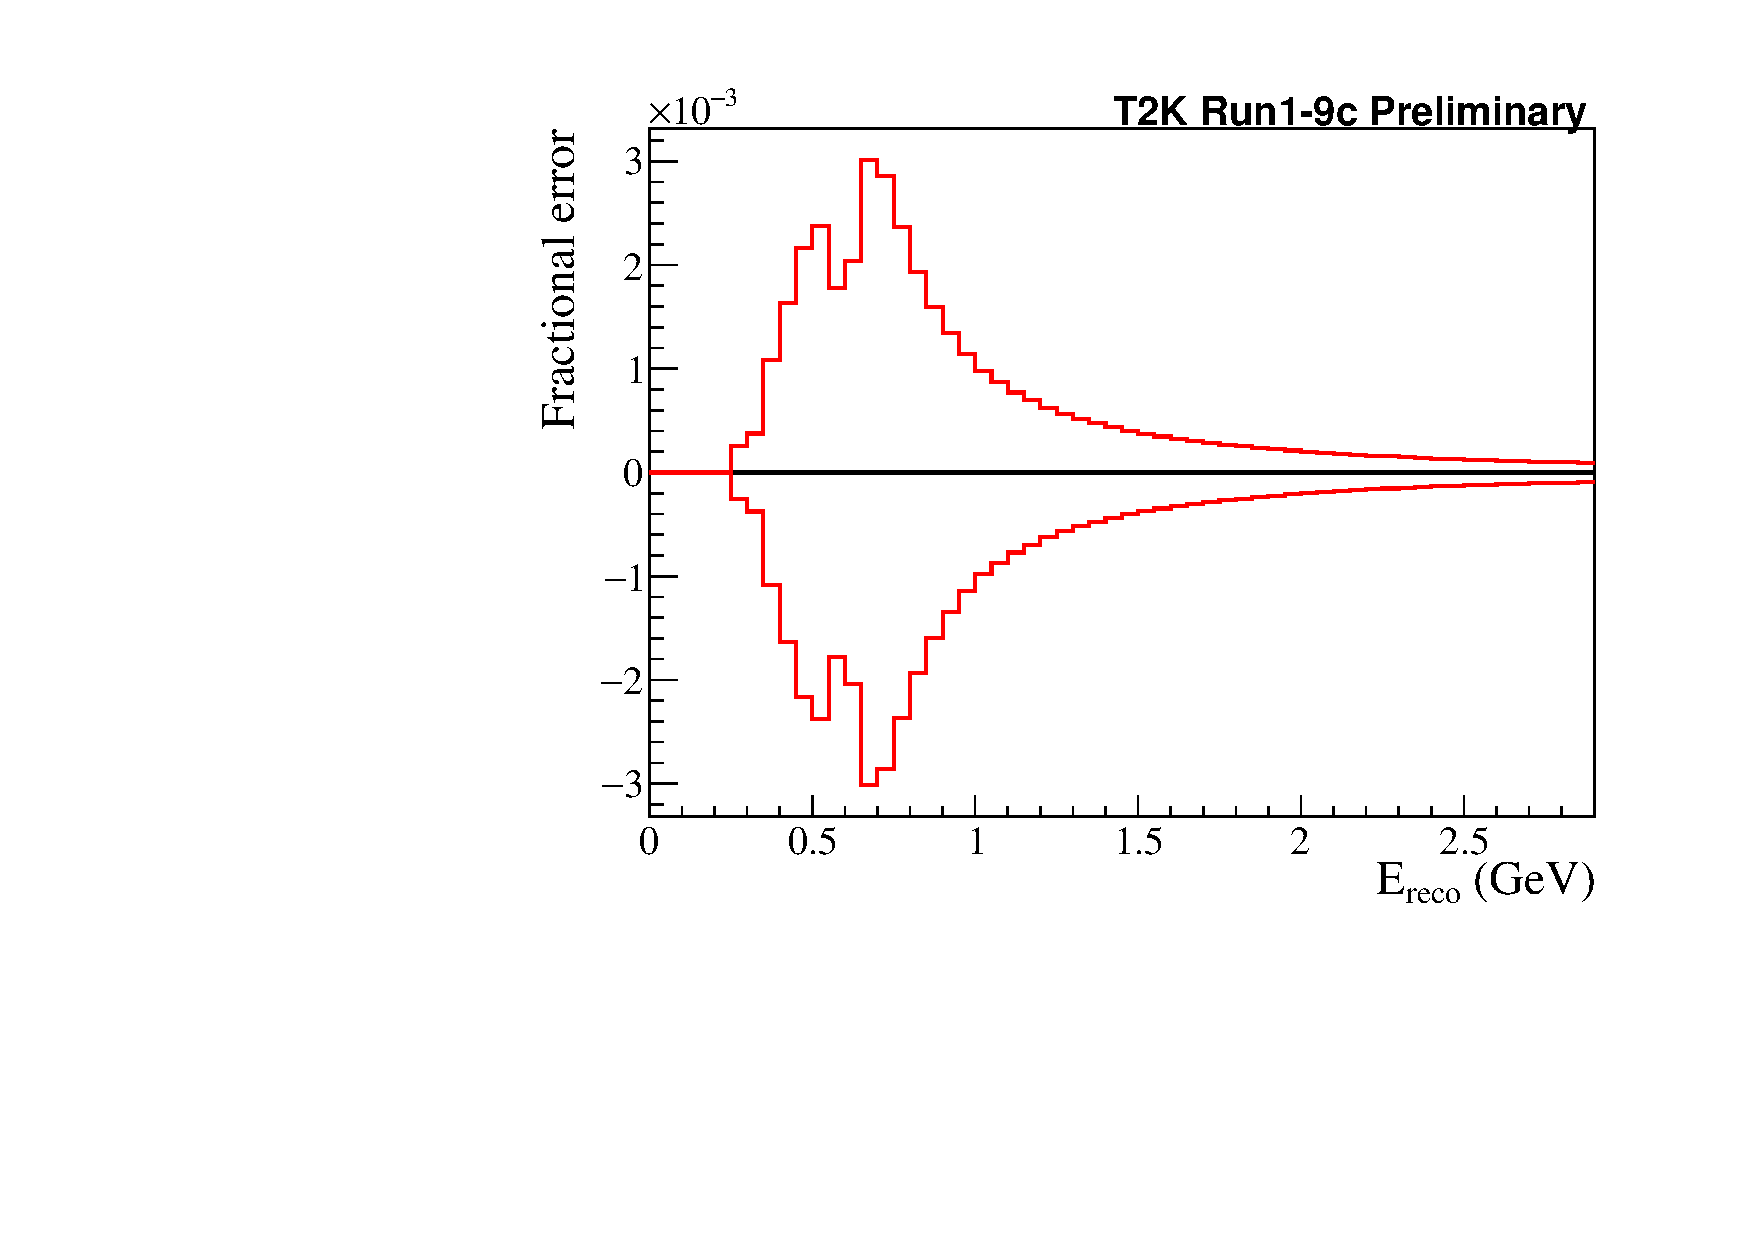
\includegraphics[width=0.9\textwidth]{images/systematics/envelopes/sk_error_table_RHC1Rmu_osc_envelope_fractional}
		\caption{Muon-like, antineutrino mode}
	\end{subfigure}
	\begin{subfigure}[b]{0.49\textwidth}
		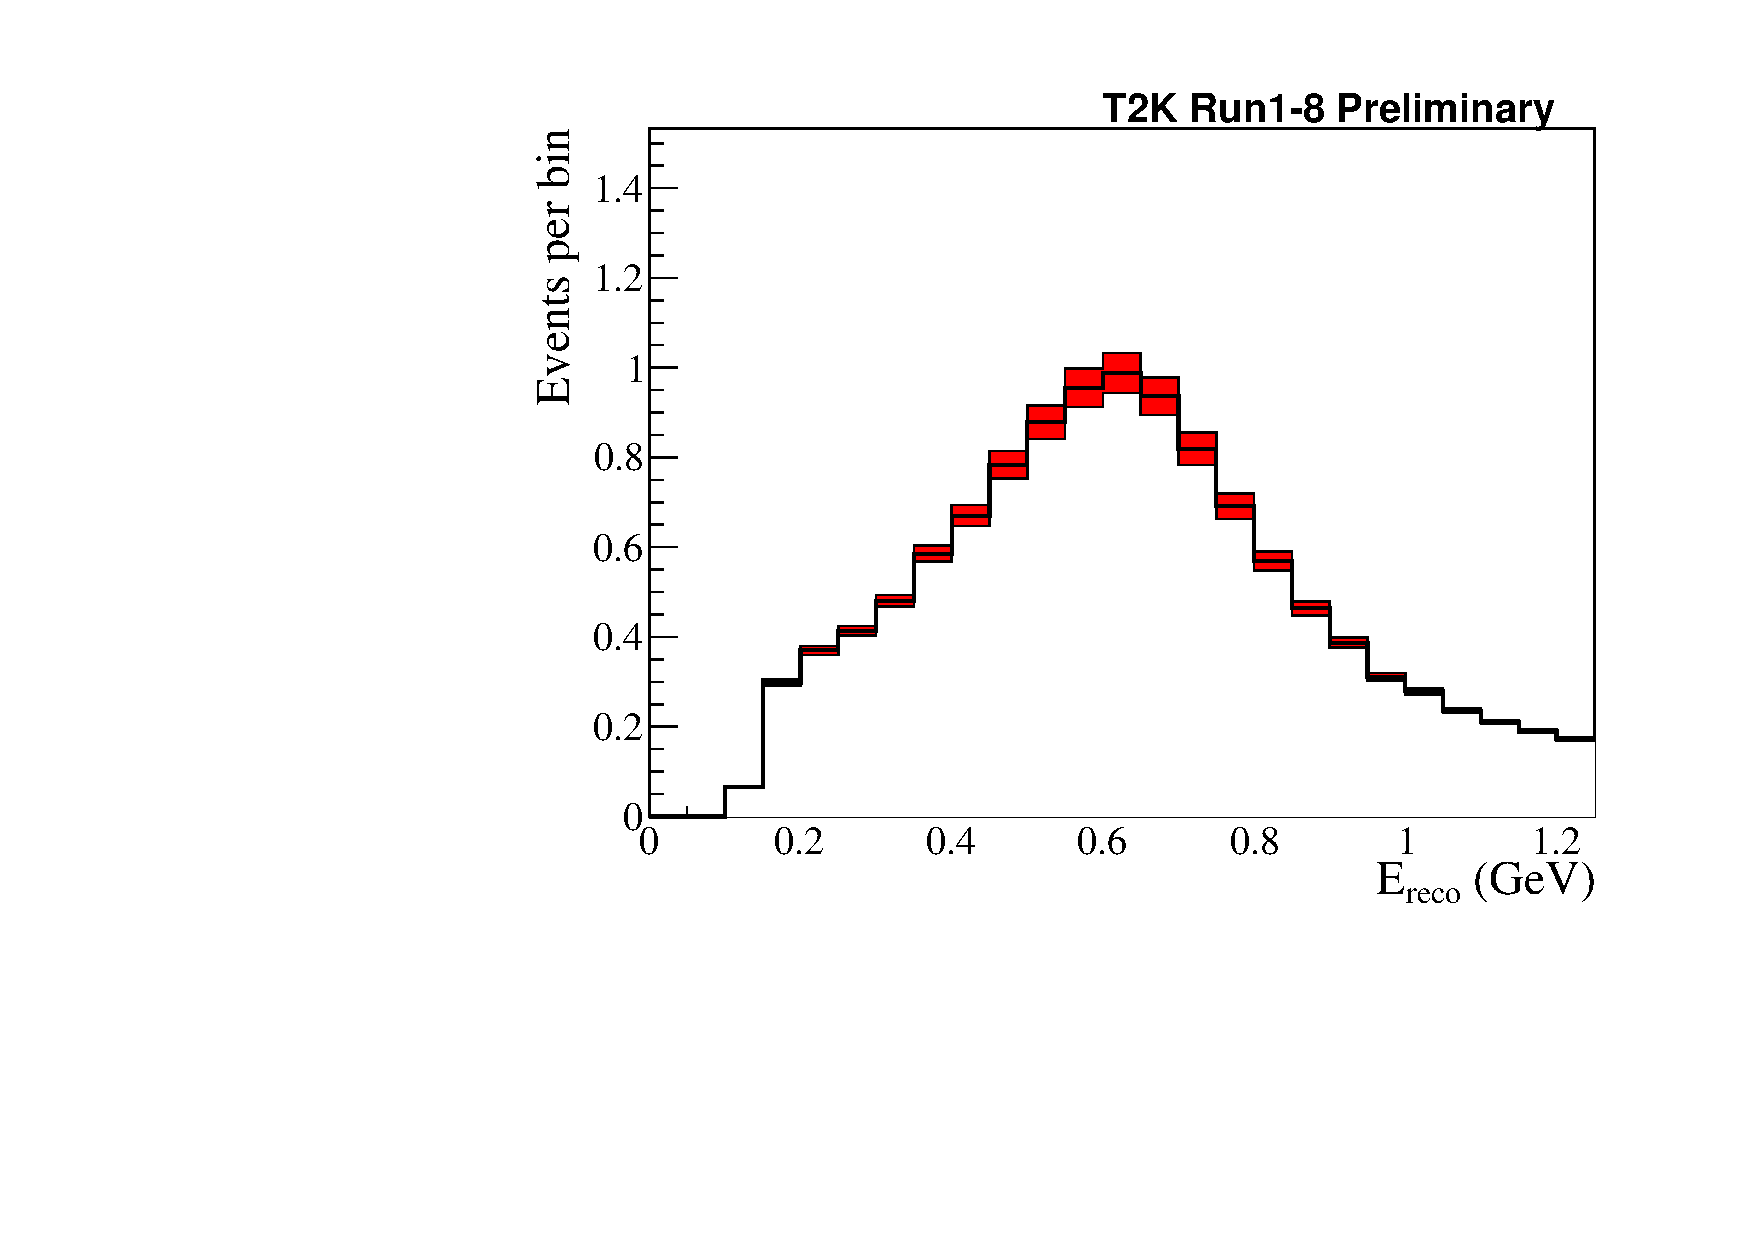
\includegraphics[width=0.9\textwidth]{images/systematics/envelopes/sk_error_table_RHC1Re_osc_envelope}
		\caption{Electron-like antineutrino mode}
	\end{subfigure}
	\begin{subfigure}[b]{0.49\textwidth}
		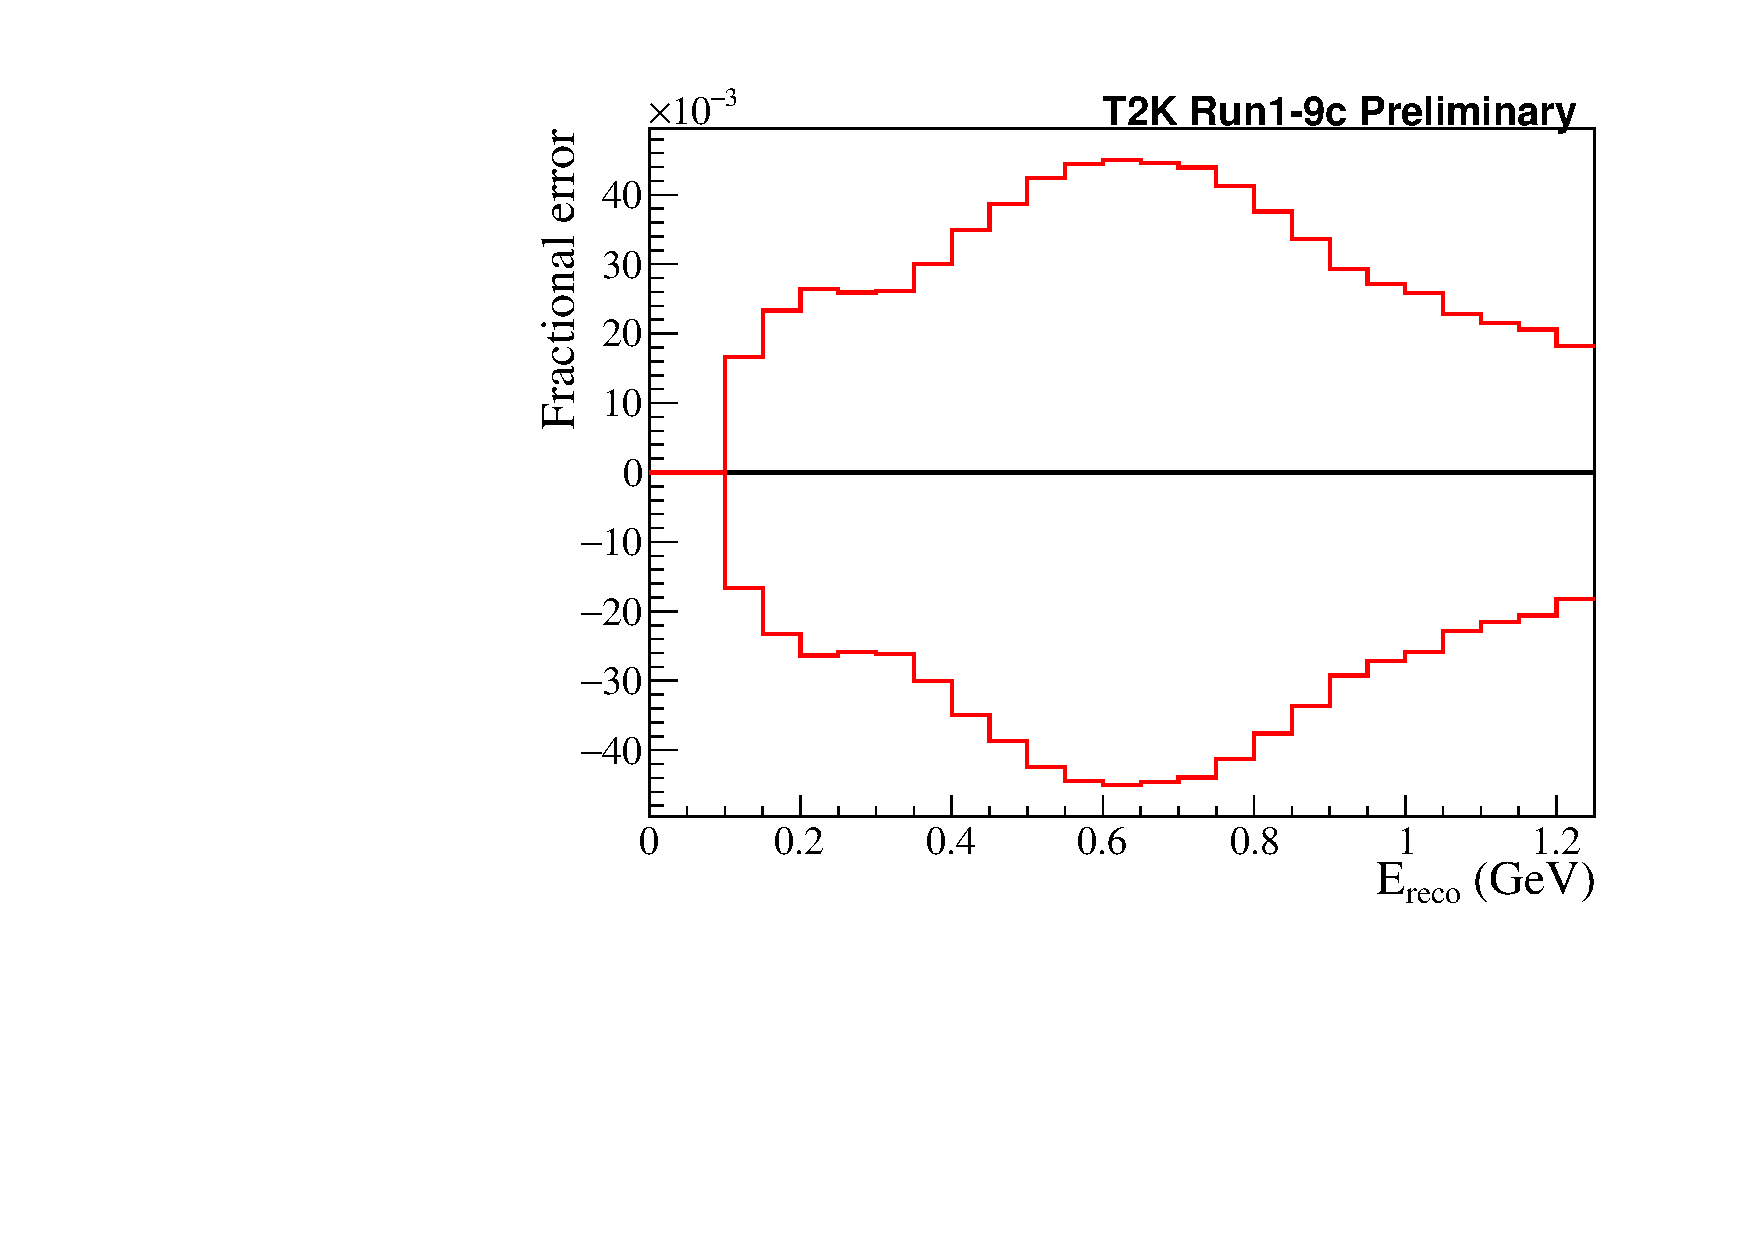
\includegraphics[width=0.9\textwidth]{images/systematics/envelopes/sk_error_table_RHC1Re_osc_envelope_fractional}
		\caption{Electron-like antineutrino mode}
	\end{subfigure}
	\caption {
		Error envelopes (left) and fractional errors (right) for the reconstructed neutrino energy spectrum for all oscillation nuisance parameters. \NumToysSmall toys are generated for the Asimov data set A with randomized systematic parameters with correlations taken into account. Since \deltacp, \ssqthtwothree, \dmsqtwothree and the mass hierarchy will be measured, only the uncertainty on \ssqthonethree, \ssqthonetwo and \dmsqonetwo are taken into account.
	}
	\label{fig:sk_envelopes_osc_b}
\end{figure*}
\clearpage
\begin{figure*}
	\center
	\begin{subfigure}[b]{0.49\textwidth}
		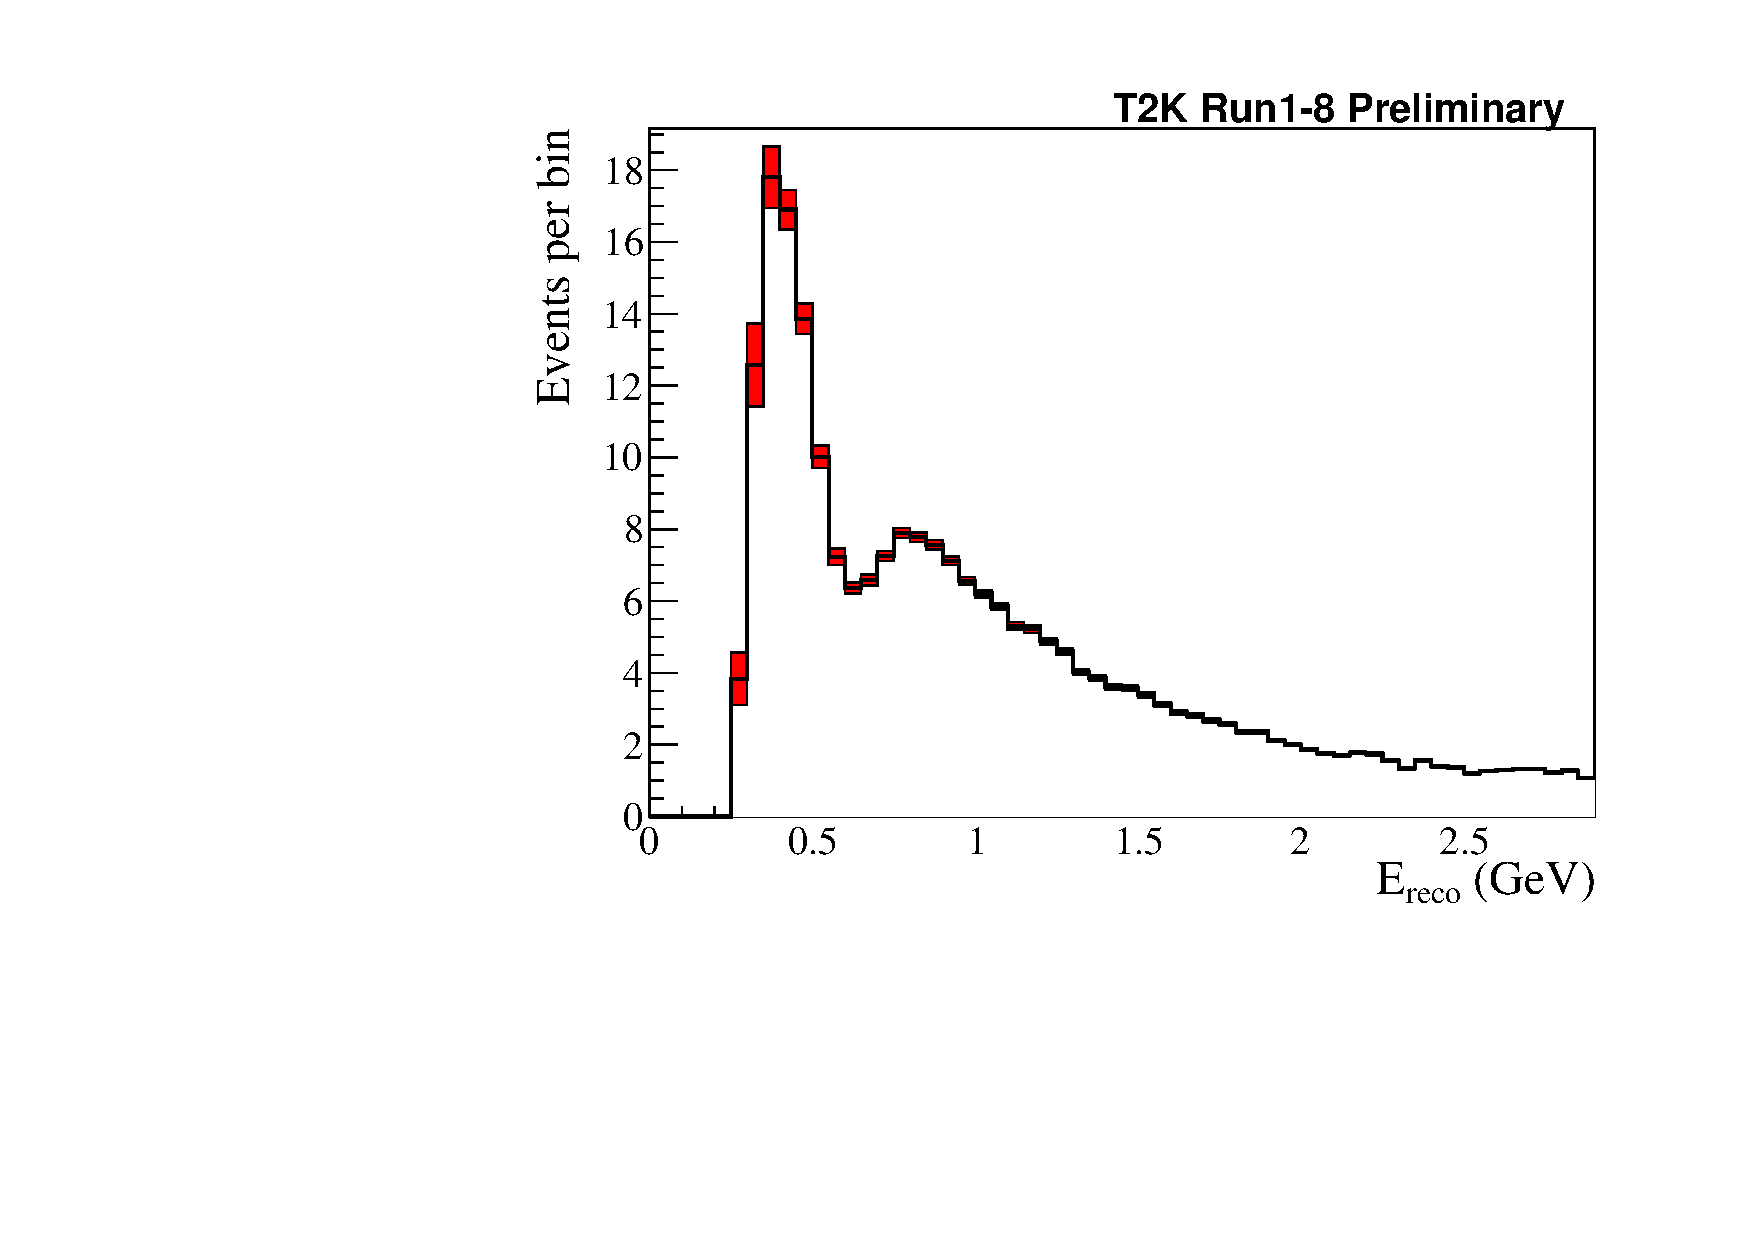
\includegraphics[width=0.9\textwidth]{images/systematics/envelopes/sk_error_table_1Rmu_skdet_envelope}
		\caption{Muon-like, neutrino mode}
	\end{subfigure}
	\begin{subfigure}[b]{0.49\textwidth}
		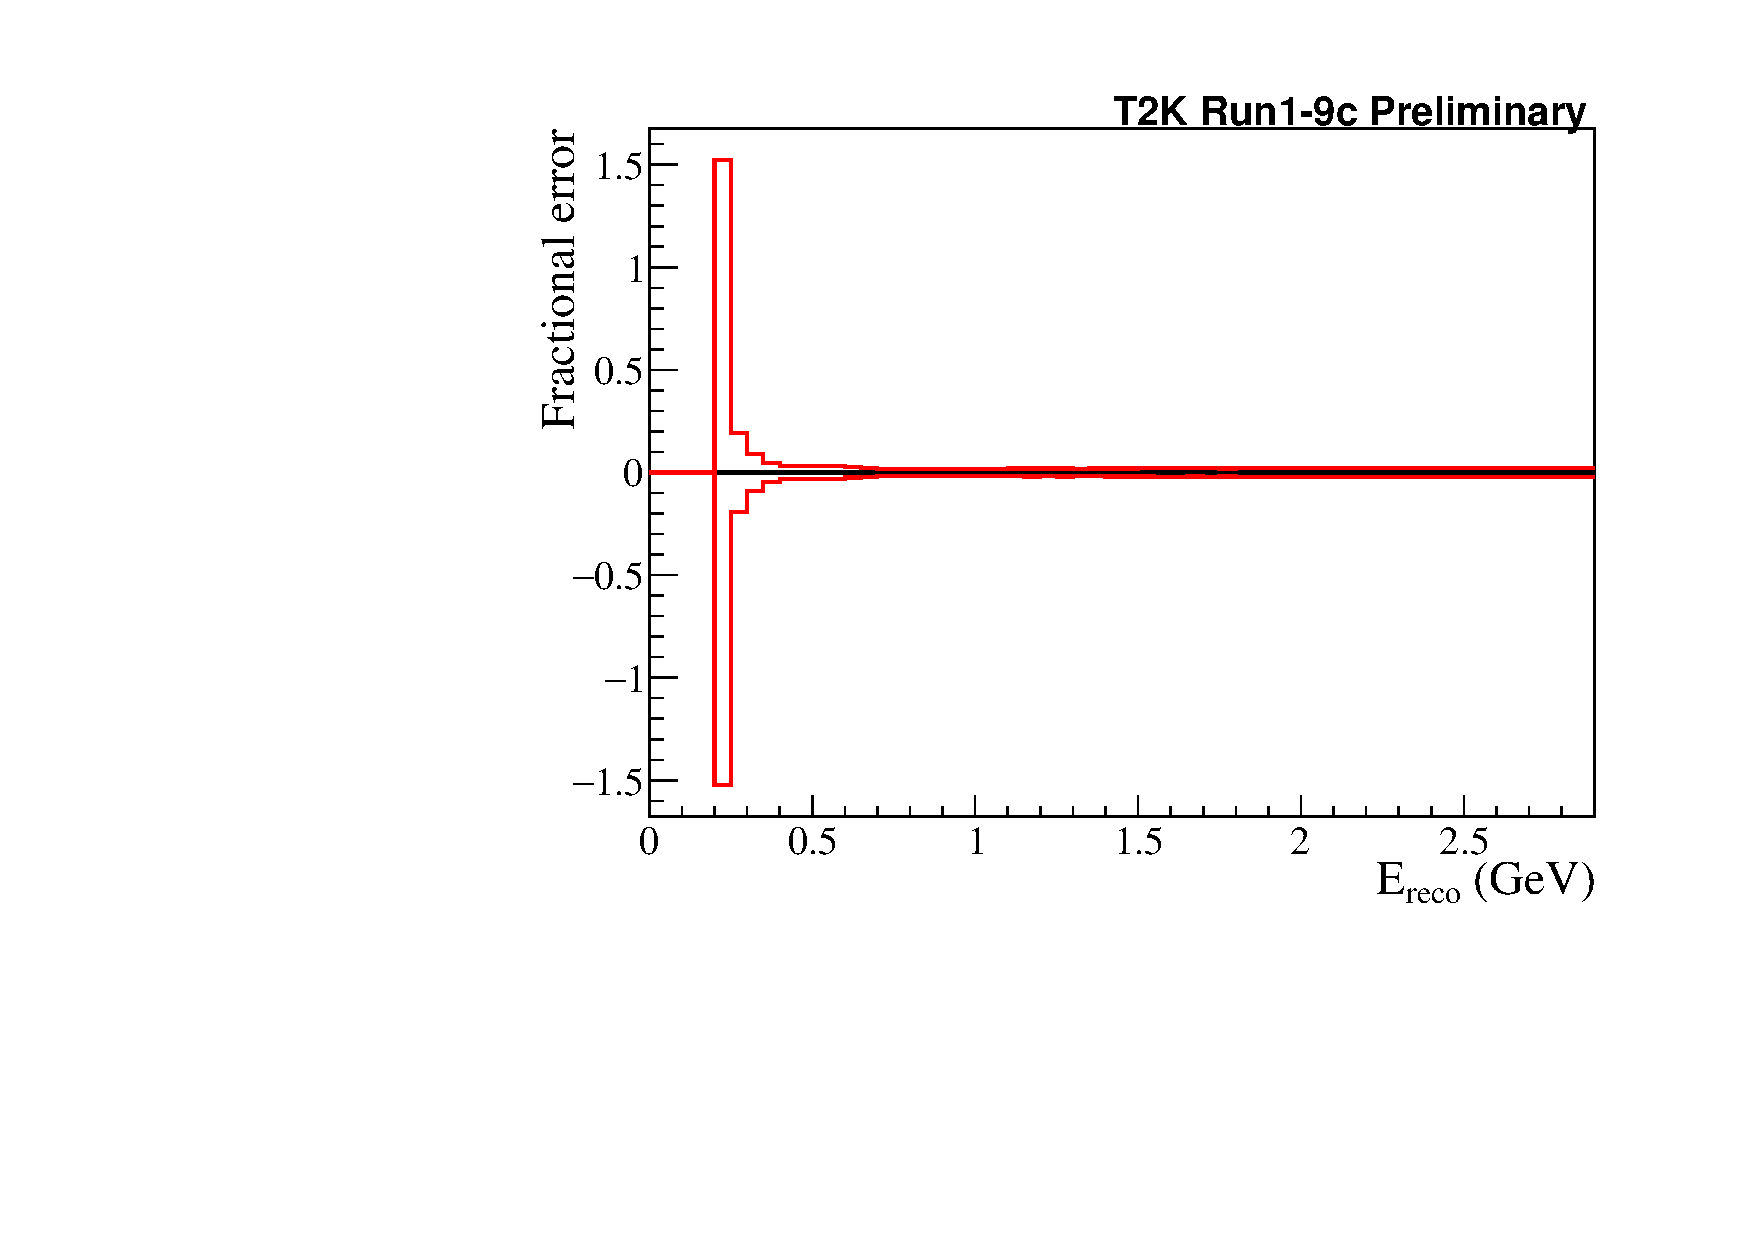
\includegraphics[width=0.9\textwidth]{images/systematics/envelopes/sk_error_table_1Rmu_skdet_envelope_fractional}
		\caption{Muon-like, neutrino mode}
	\end{subfigure}
	\begin{subfigure}[b]{0.49\textwidth}
		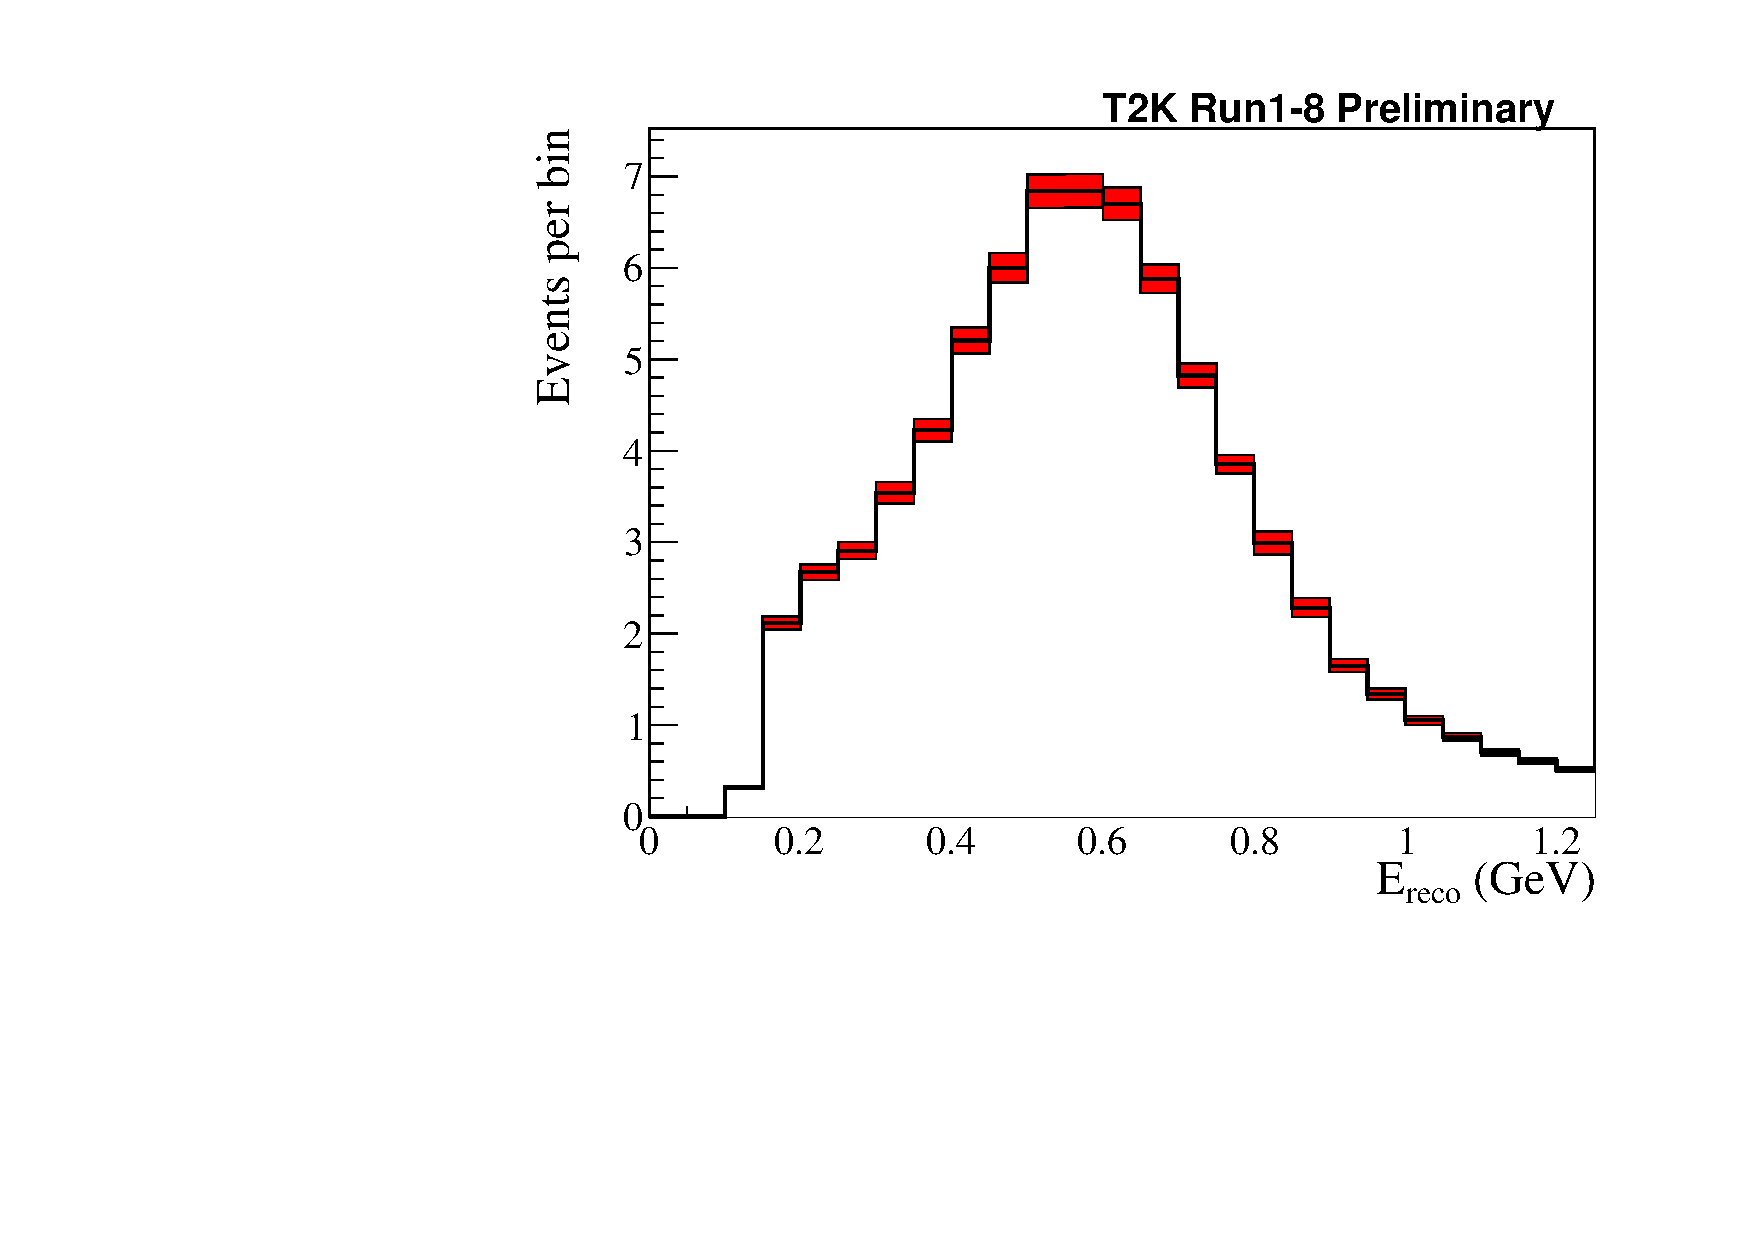
\includegraphics[width=0.9\textwidth]{images/systematics/envelopes/sk_error_table_1Re_skdet_envelope}
		\caption{Electron-like, neutrino mode}
	\end{subfigure}
	\begin{subfigure}[b]{0.49\textwidth}
		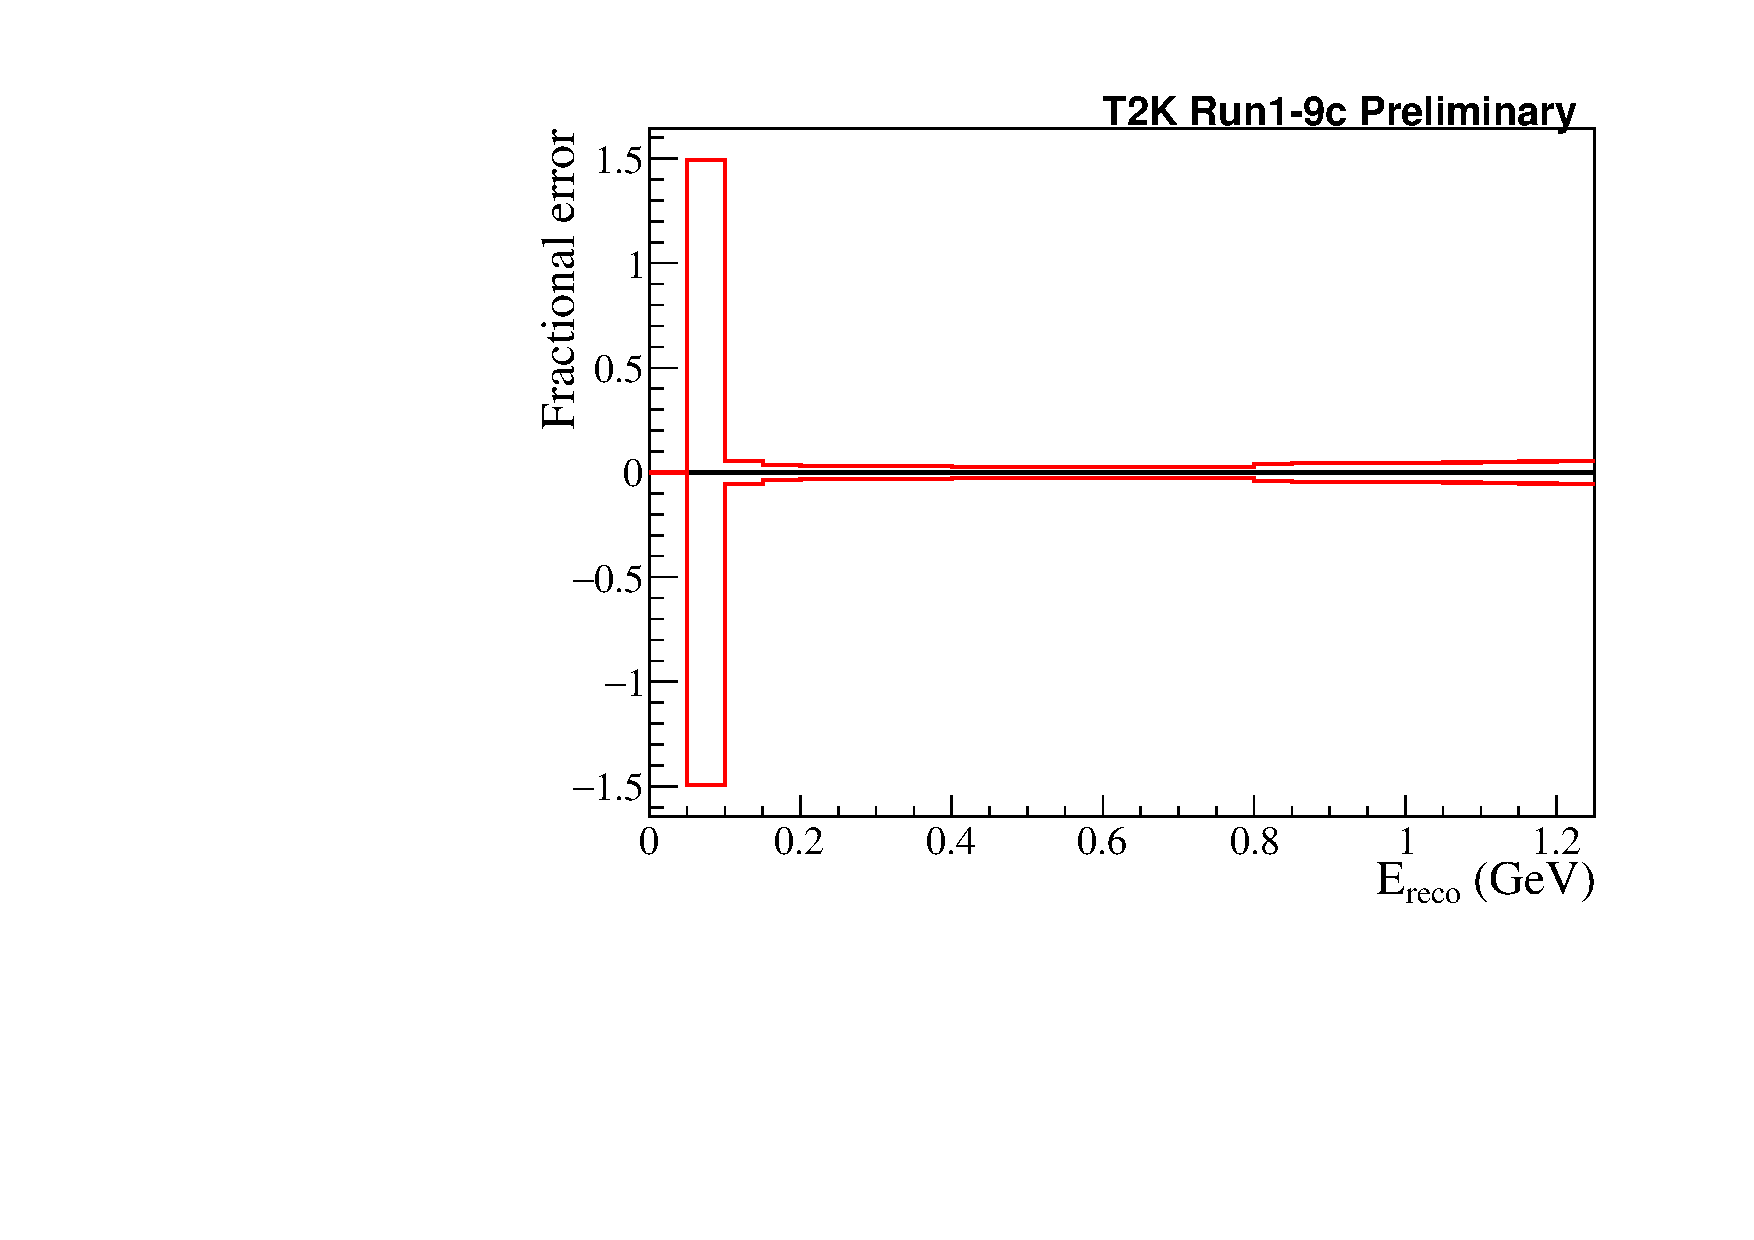
\includegraphics[width=0.9\textwidth]{images/systematics/envelopes/sk_error_table_1Re_skdet_envelope_fractional}
		\caption{Electron-like, neutrino mode}
	\end{subfigure}
	\begin{subfigure}[b]{0.49\textwidth}
		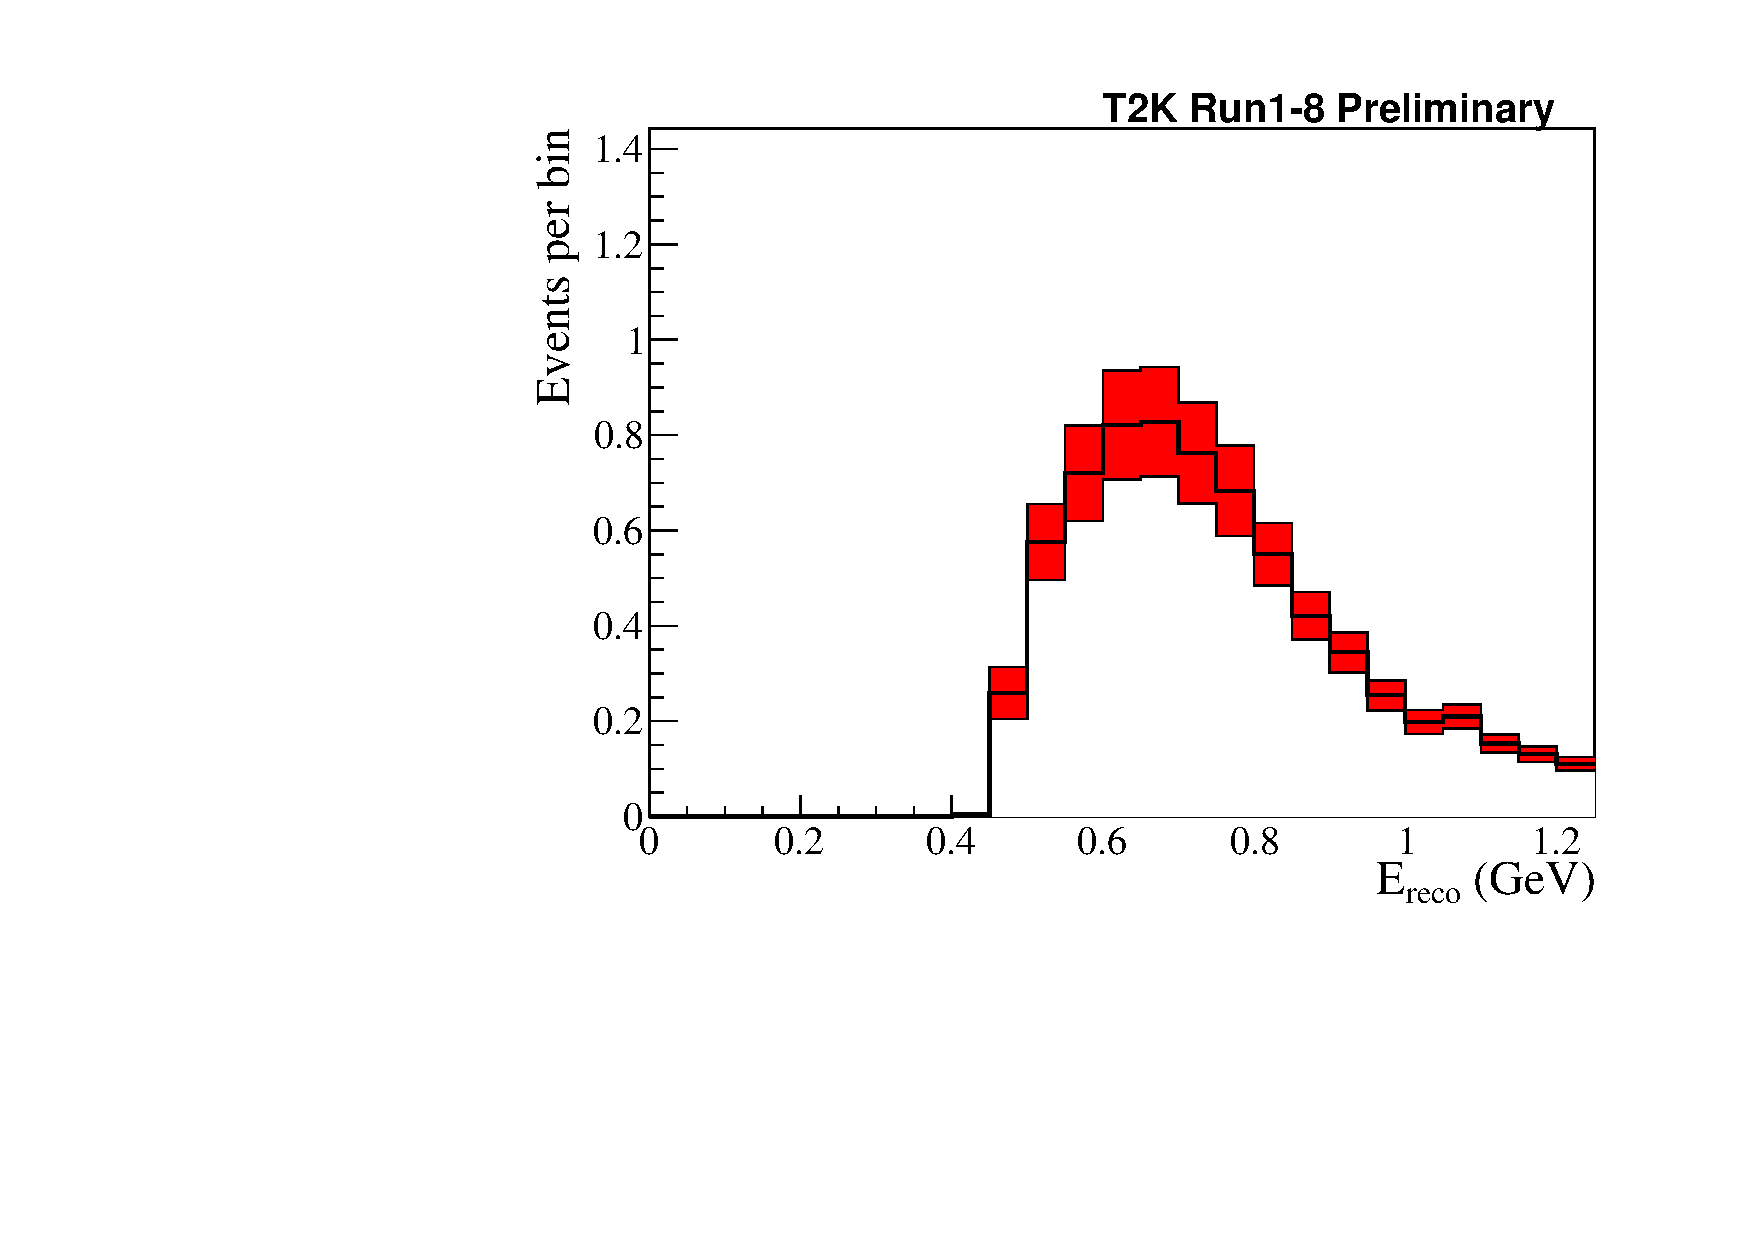
\includegraphics[width=0.9\textwidth]{images/systematics/envelopes/sk_error_table_MultiRe_skdet_envelope}
		\caption{\nueCConepi-like, neutrino mode}
	\end{subfigure}
	\begin{subfigure}[b]{0.49\textwidth}
		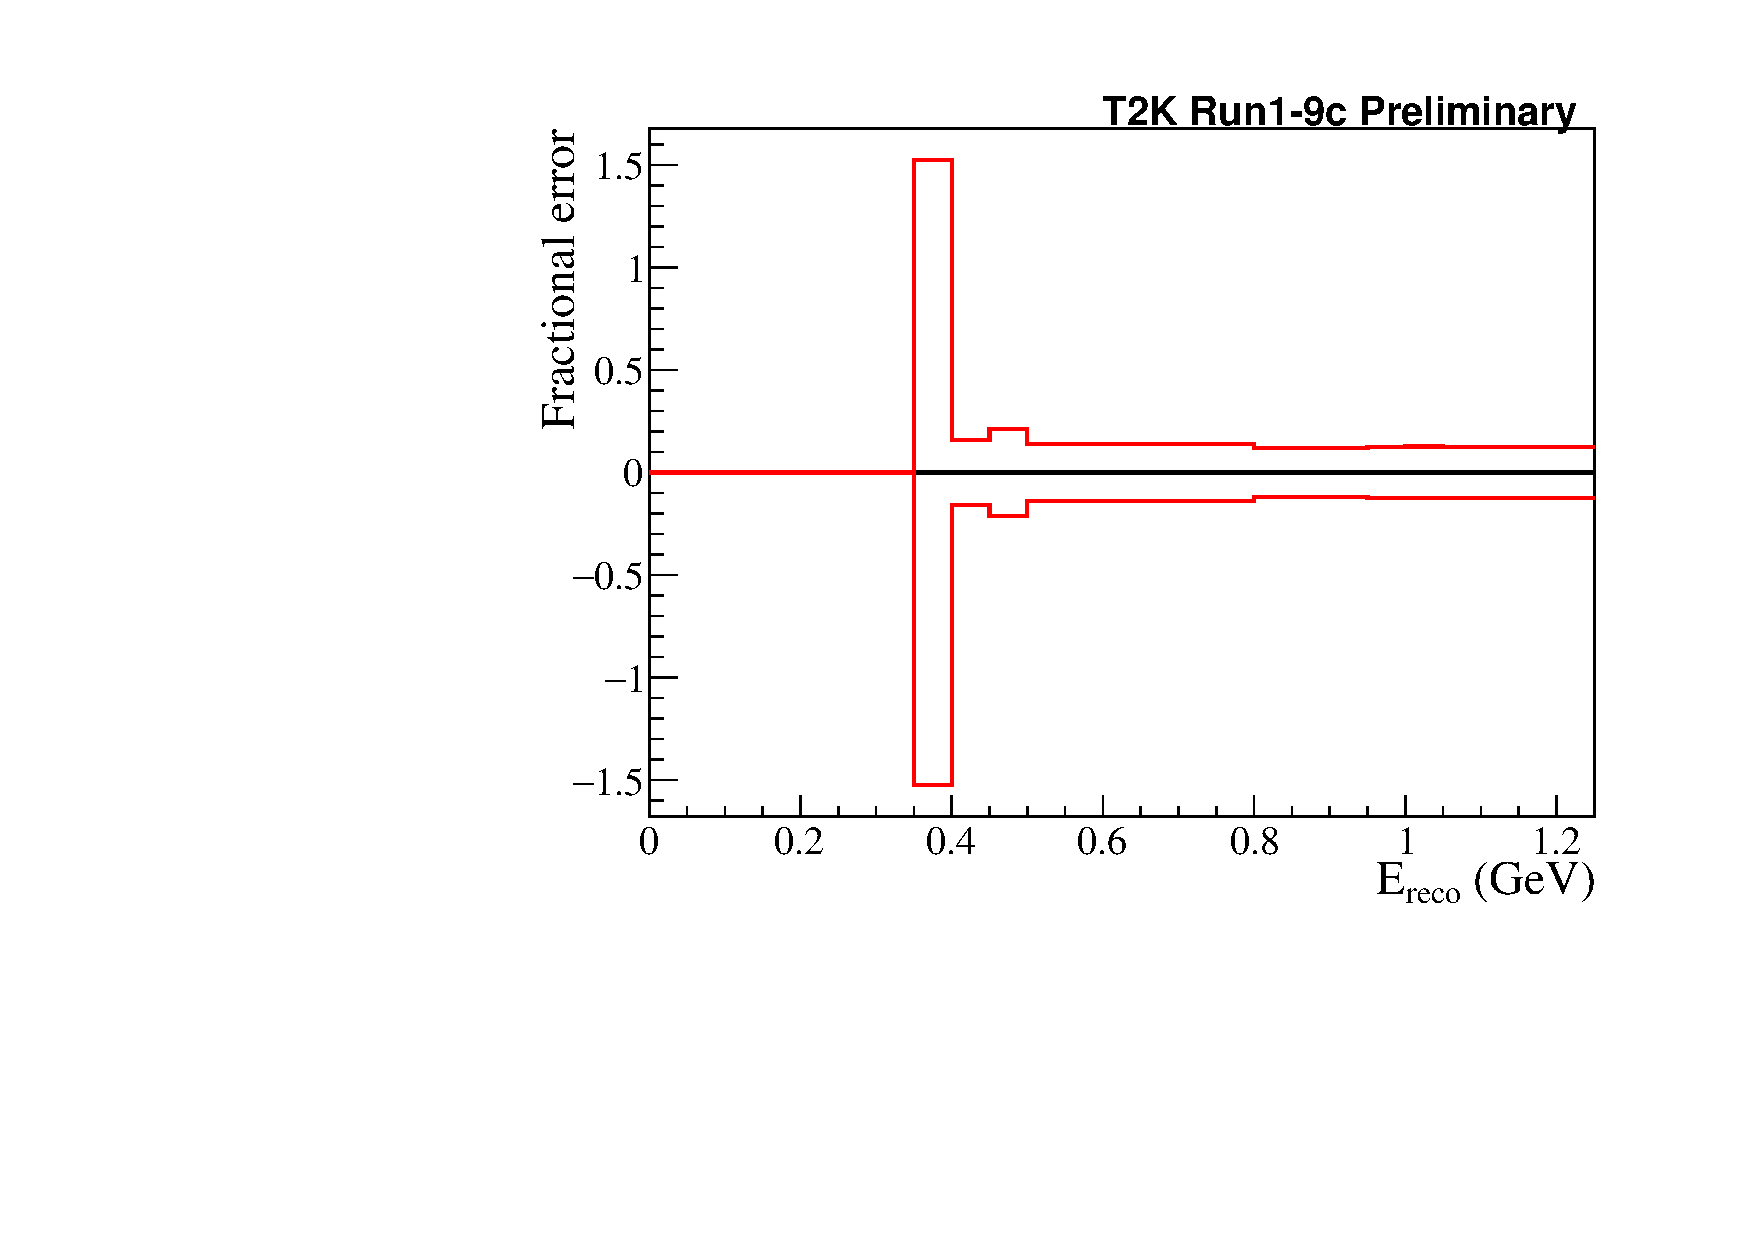
\includegraphics[width=0.9\textwidth]{images/systematics/envelopes/sk_error_table_MultiRe_skdet_envelope_fractional}
		\caption{\nueCConepi-like, neutrino mode}
	\end{subfigure}
	\caption {
		Error envelopes (left) and fractional error (right) for the reconstructed neutrino energy spectrum for Super-K detector systematic parameters. \NumToysSmall toys are generated for the Asimov data set A with randomized systematic parameters with correlations taken into account.
	}
	\label{fig:sk_envelopes_skdet}
\end{figure*}
\clearpage

\begin{figure*}
	\center
	\begin{subfigure}[b]{0.49\textwidth}
		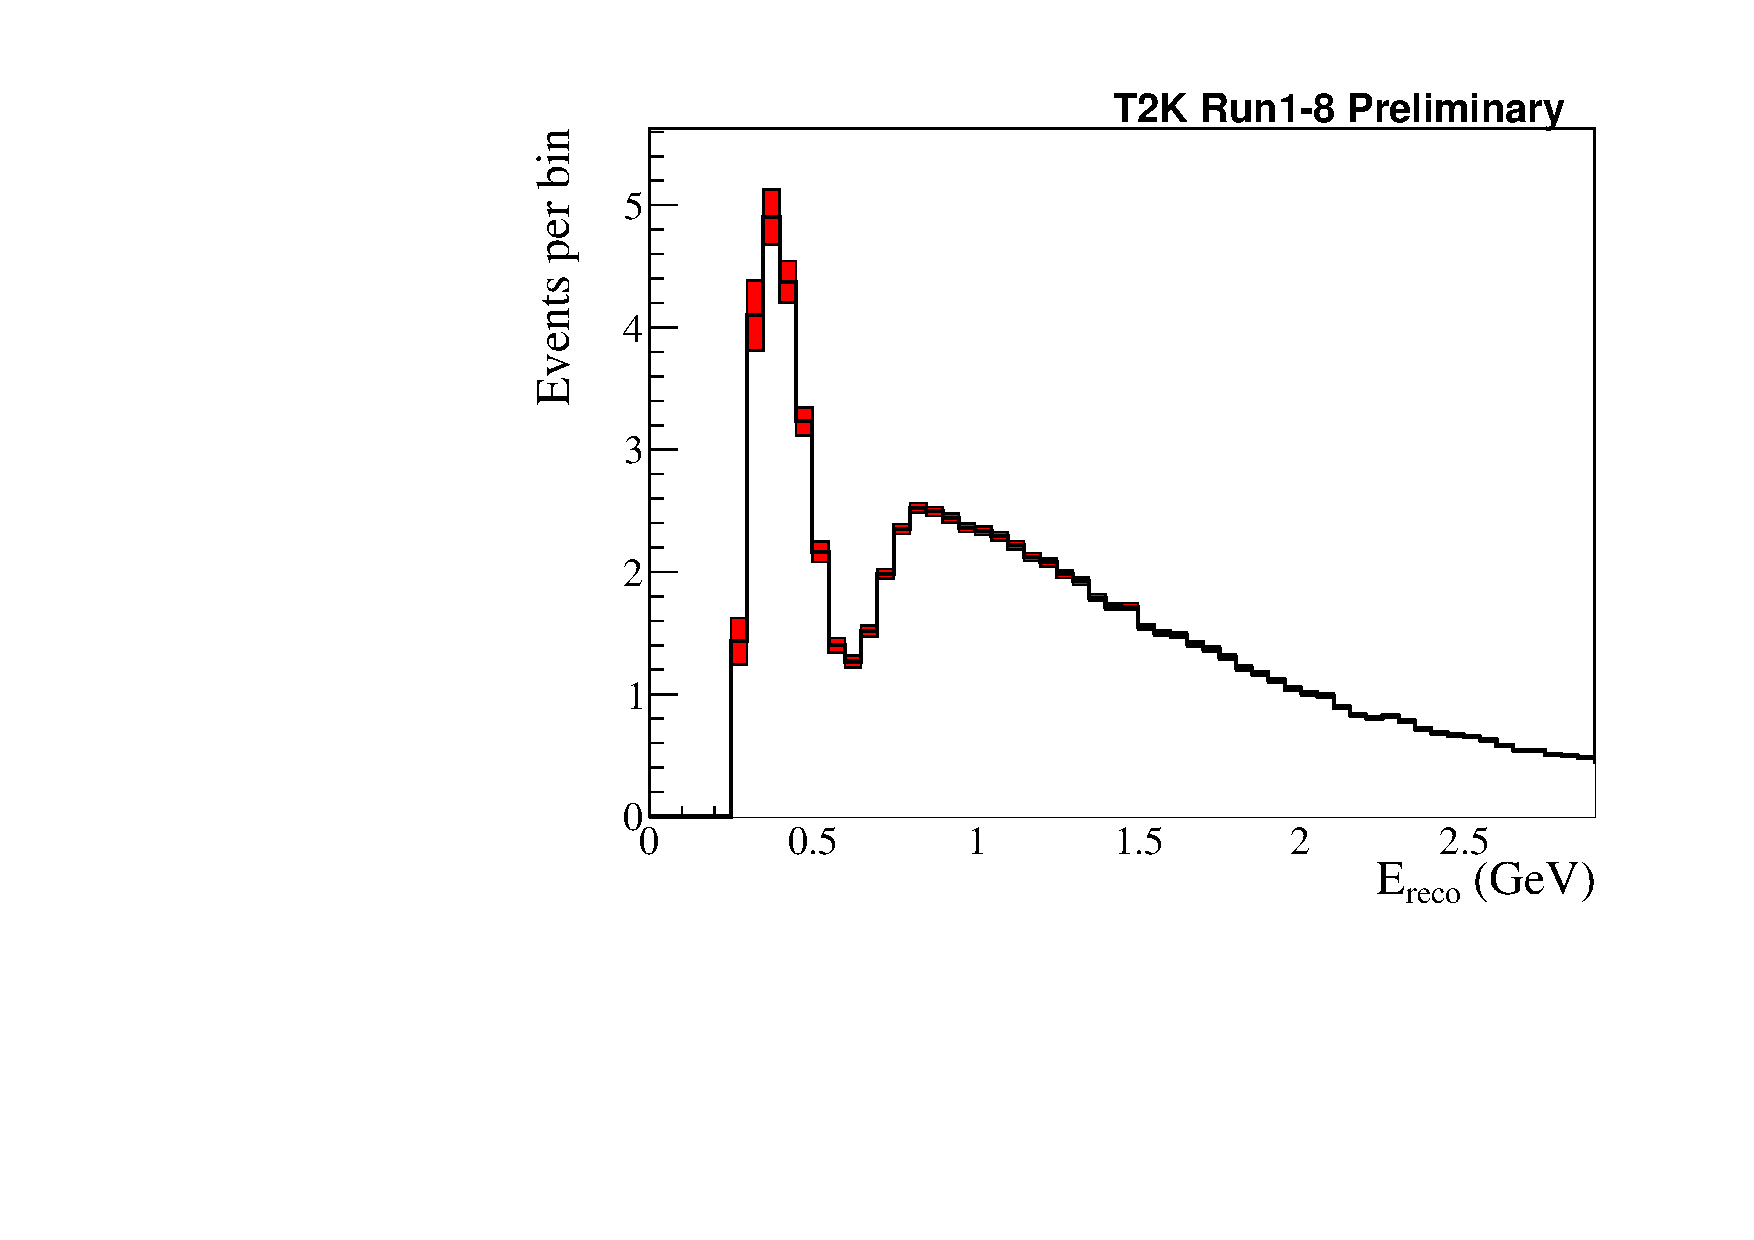
\includegraphics[width=0.9\textwidth]{images/systematics/envelopes/sk_error_table_RHC1Rmu_skdet_envelope}
		\caption{Muon-like, antineutrino mode}
	\end{subfigure}
	\begin{subfigure}[b]{0.49\textwidth}
		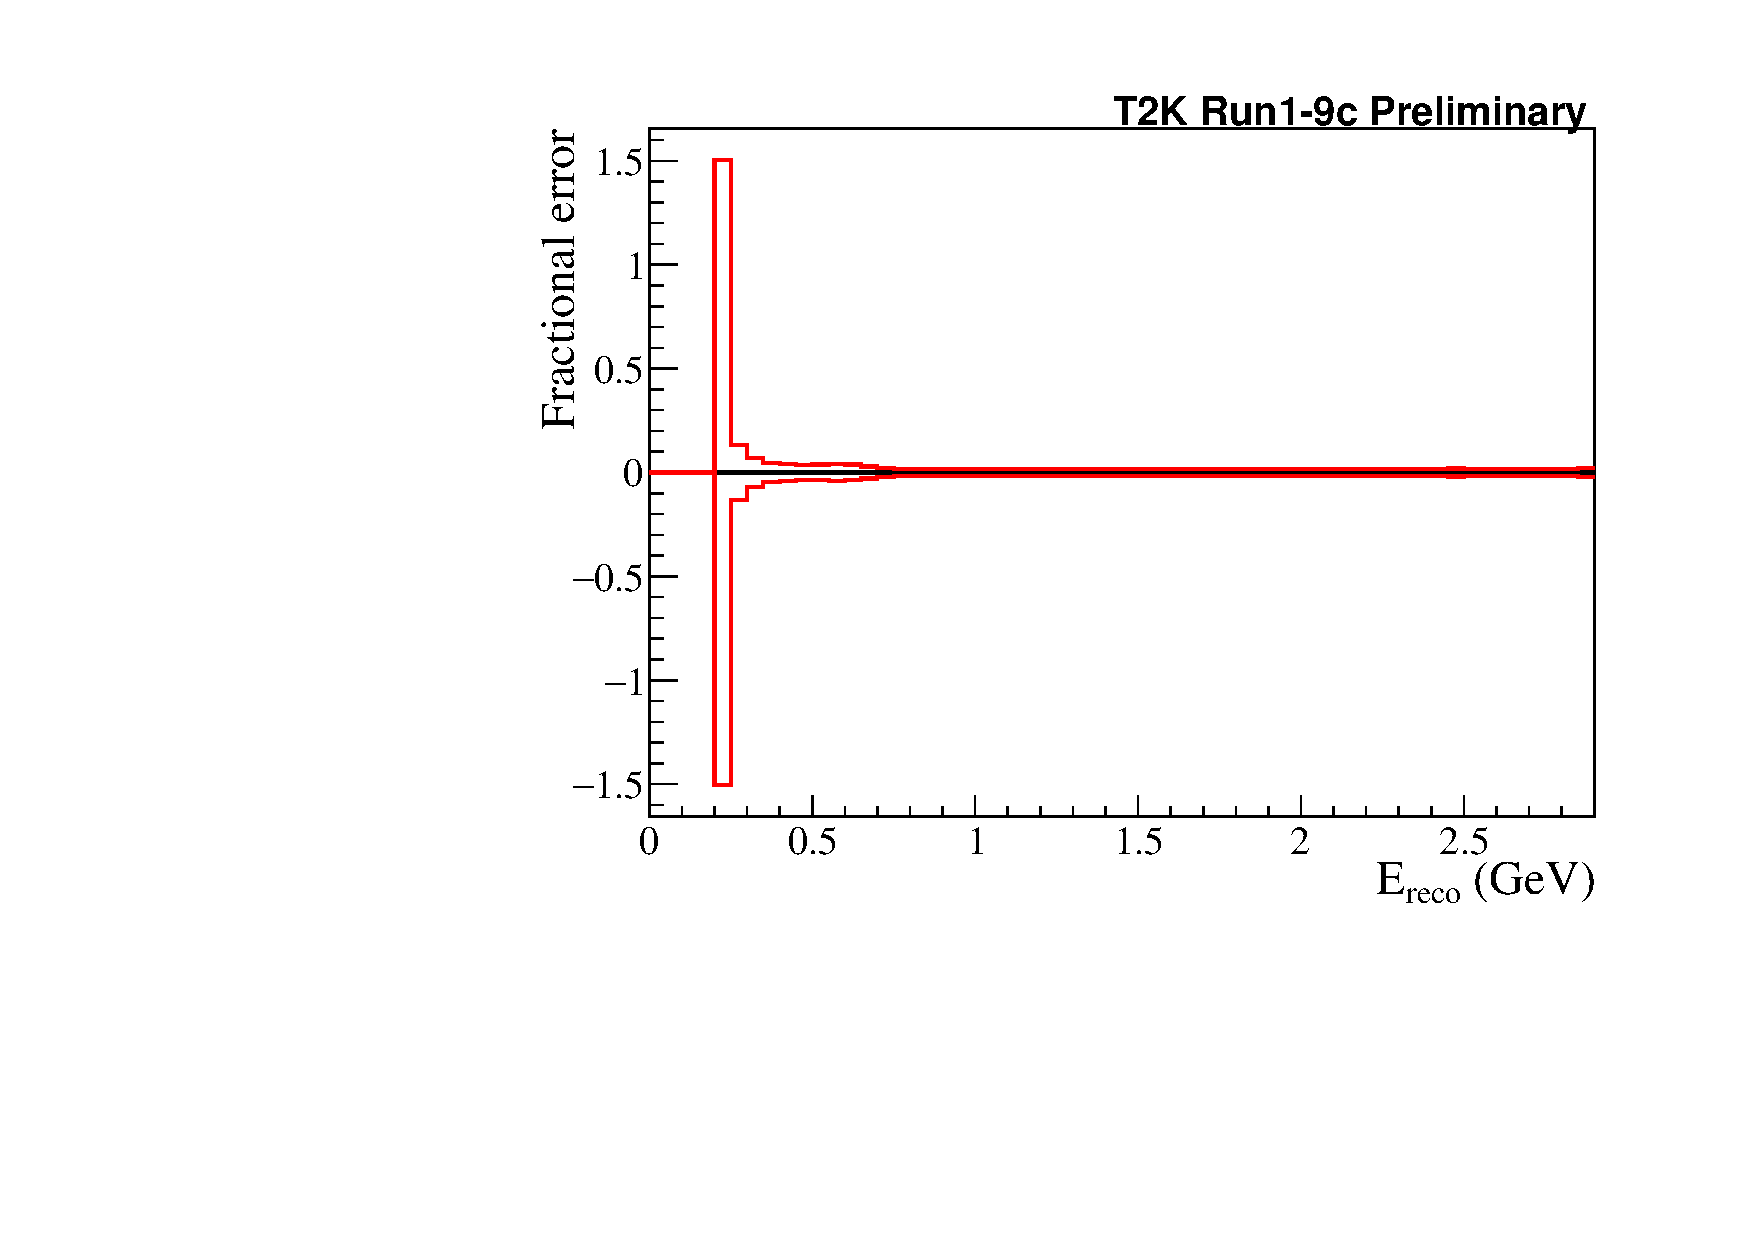
\includegraphics[width=0.9\textwidth]{images/systematics/envelopes/sk_error_table_RHC1Rmu_skdet_envelope_fractional}
		\caption{Muon-like, antineutrino mode}
	\end{subfigure}
	\begin{subfigure}[b]{0.49\textwidth}
		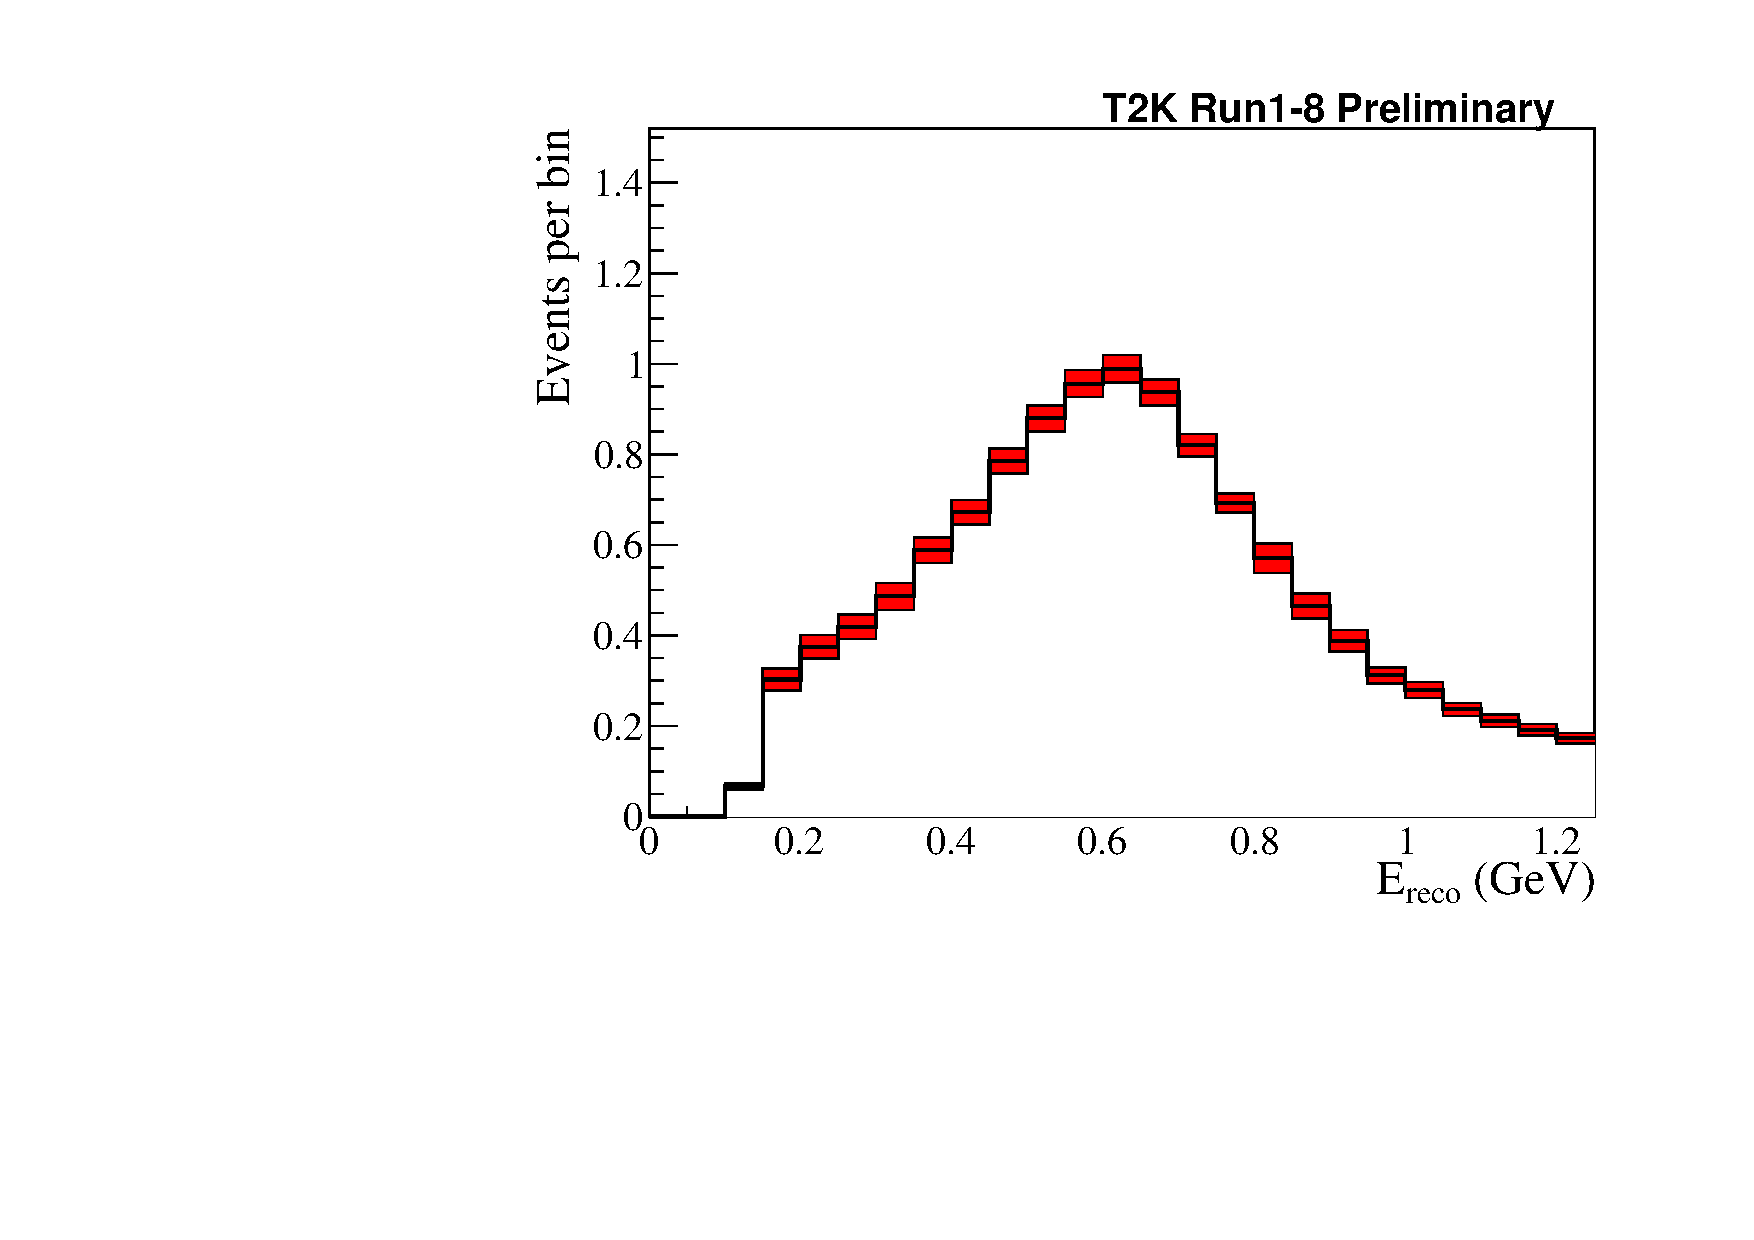
\includegraphics[width=0.9\textwidth]{images/systematics/envelopes/sk_error_table_RHC1Re_skdet_envelope}
		\caption{Electron-like antineutrino mode}
	\end{subfigure}
	\begin{subfigure}[b]{0.49\textwidth}
		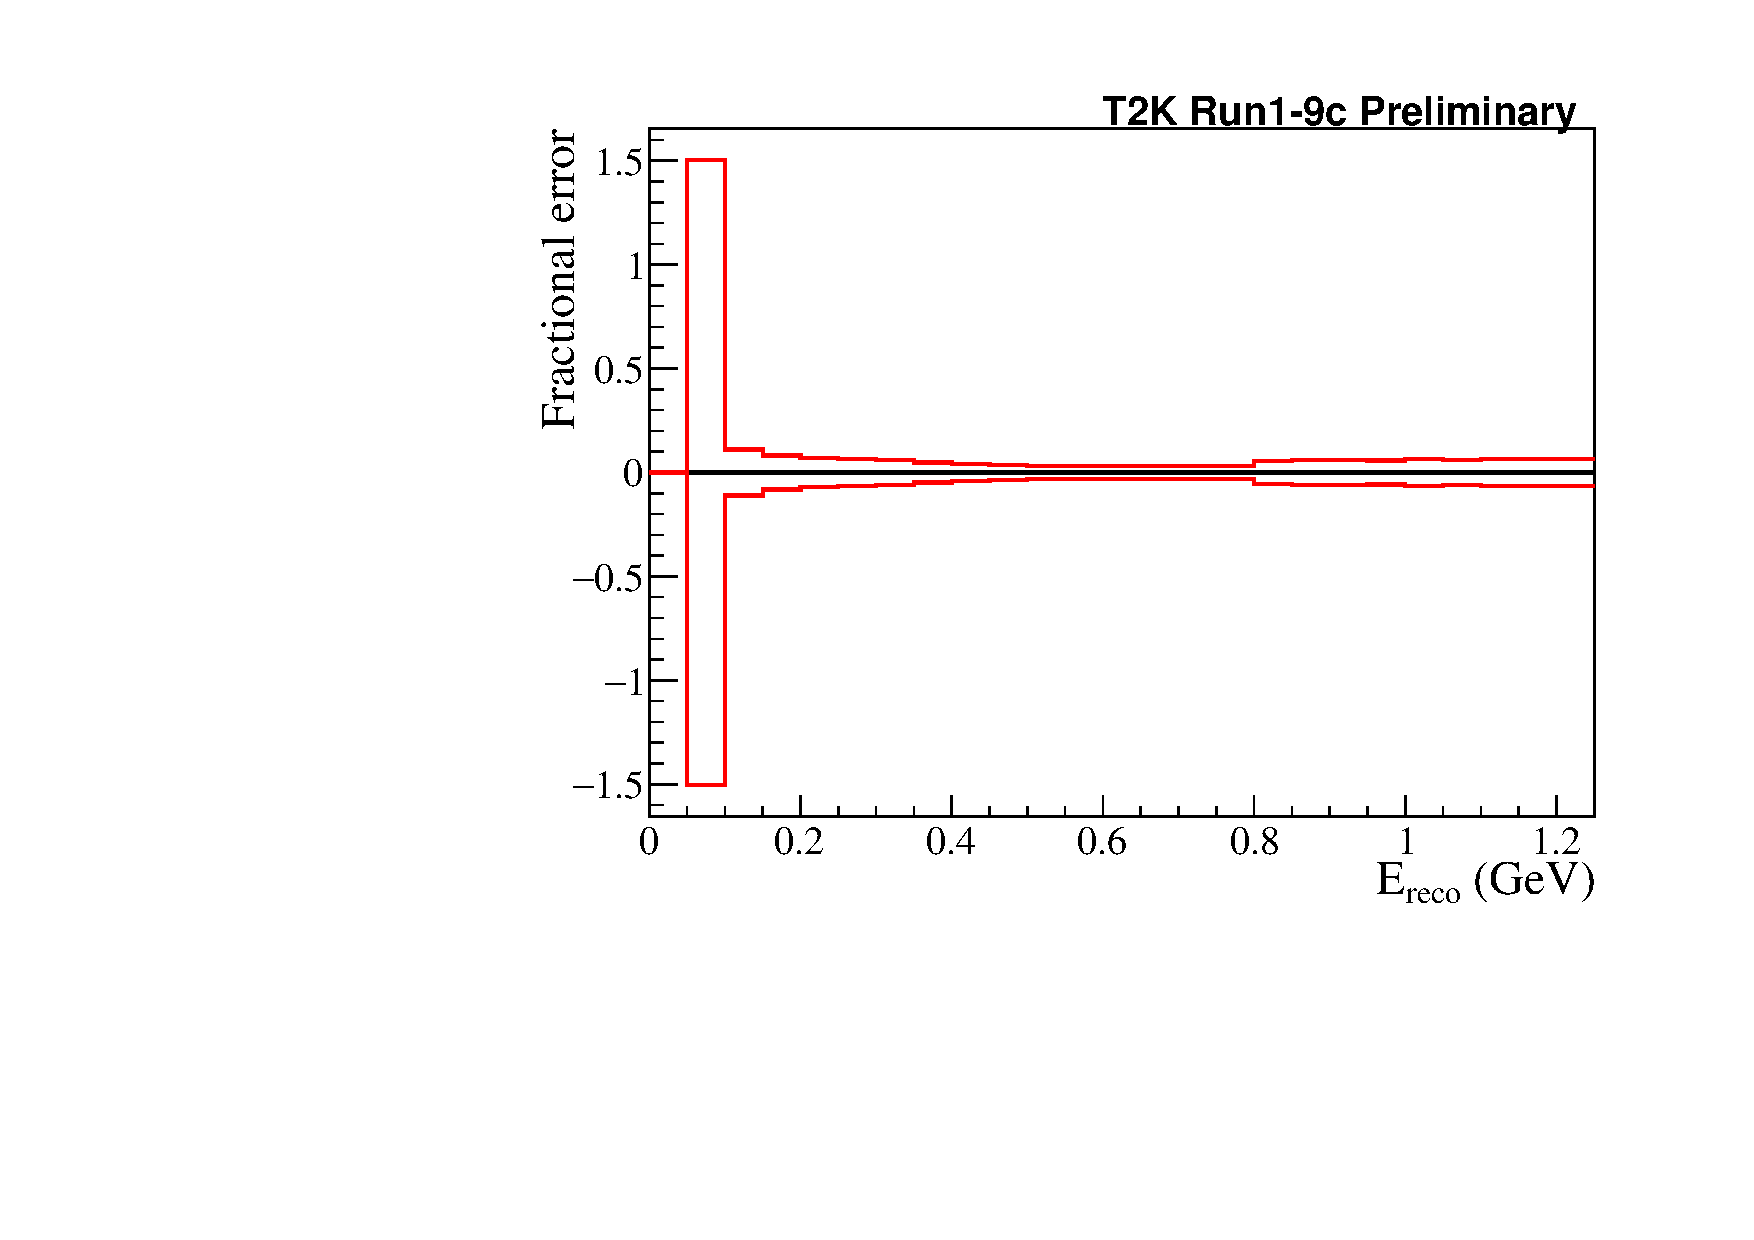
\includegraphics[width=0.9\textwidth]{images/systematics/envelopes/sk_error_table_RHC1Re_skdet_envelope_fractional}
		\caption{Electron-like antineutrino mode}
	\end{subfigure}
	\caption {
		Error envelopes (left) and fractional error (right) for the reconstructed neutrino energy spectrum for Super-K detector systematic parameters. \NumToysSmall toys are generated for the Asimov data set A with randomized systematic parameters with correlations taken into account.
	}
	\label{fig:sk_envelopes_skdet_b}
\end{figure*}
\clearpage
\begin{figure*}
	\center
	\begin{subfigure}[b]{0.49\textwidth}
		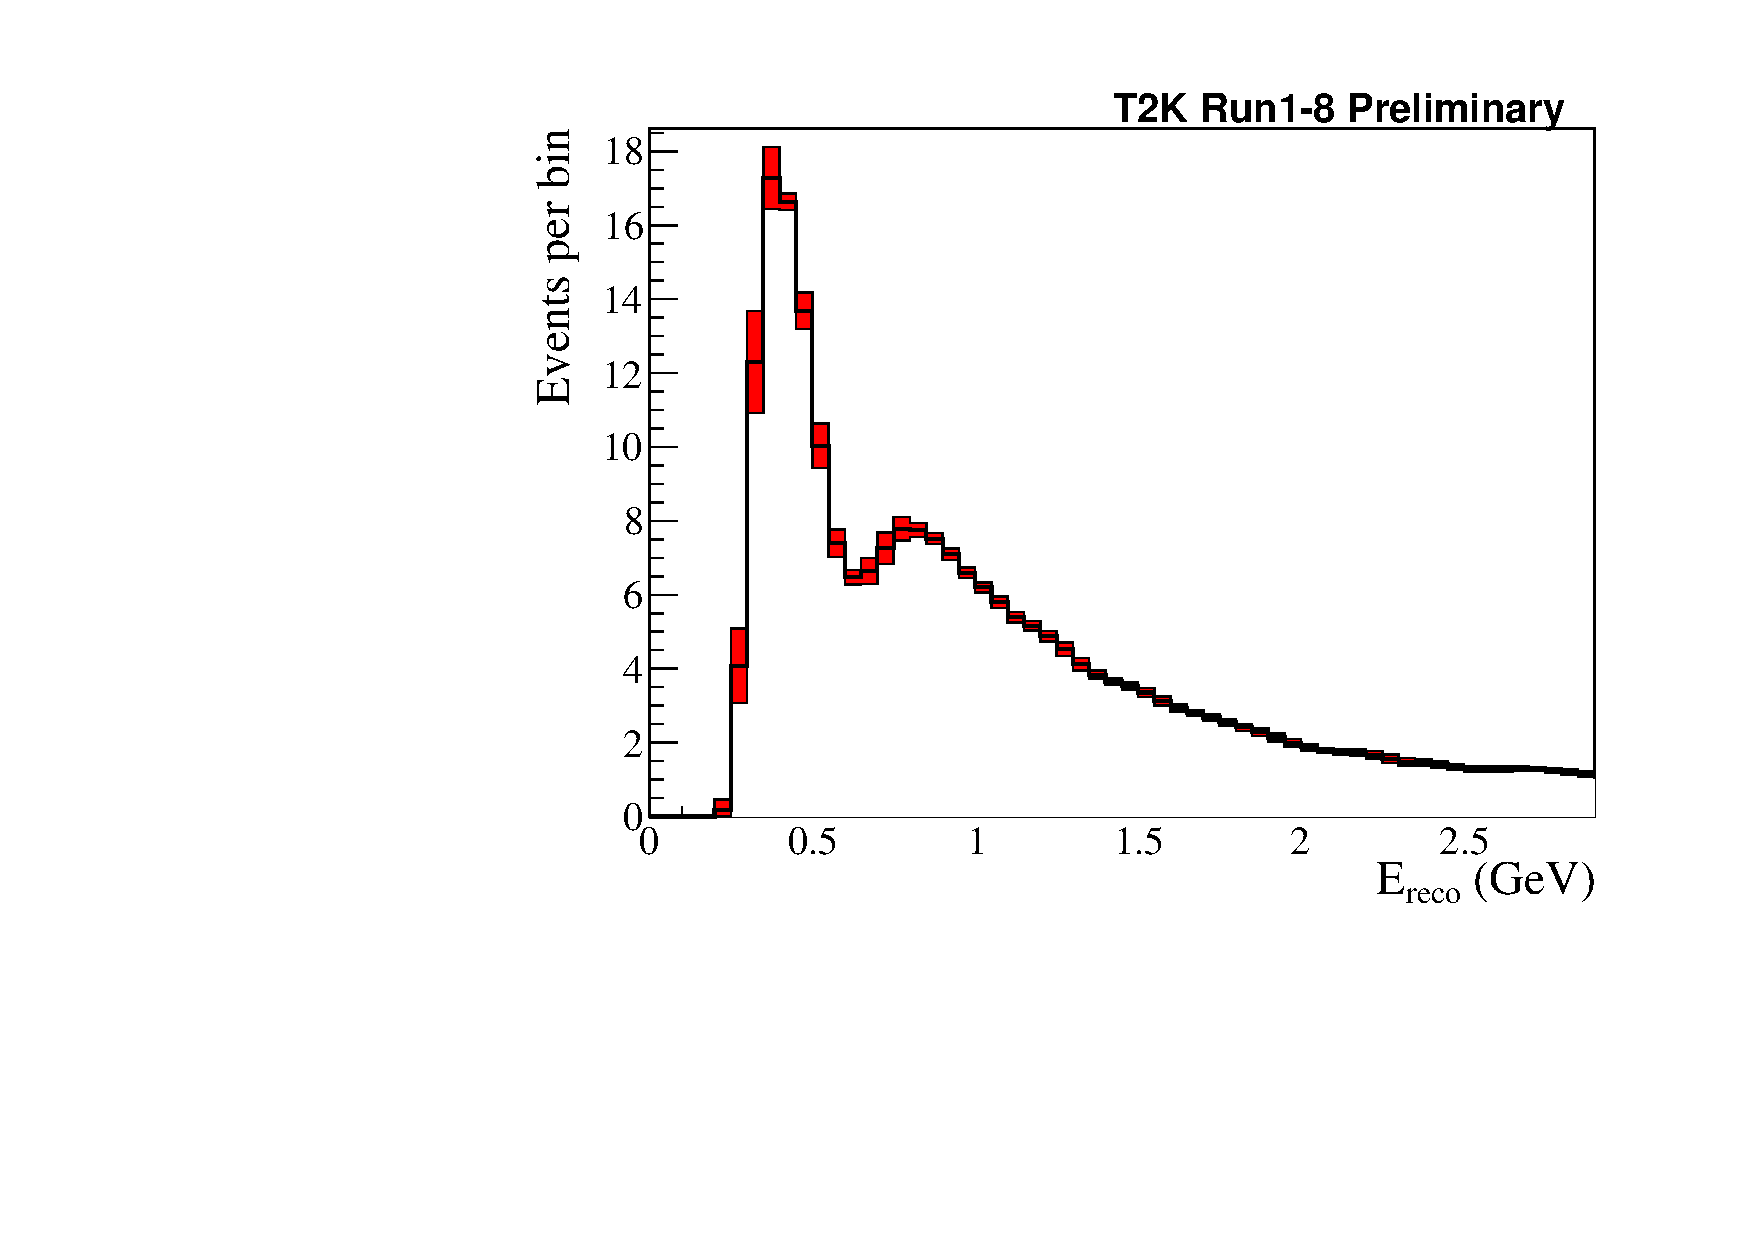
\includegraphics[width=0.9\textwidth]{images/systematics/envelopes/sk_error_table_1Rmu_skfsi_envelope}
		\caption{Muon-like, neutrino mode}
	\end{subfigure}
	\begin{subfigure}[b]{0.49\textwidth}
		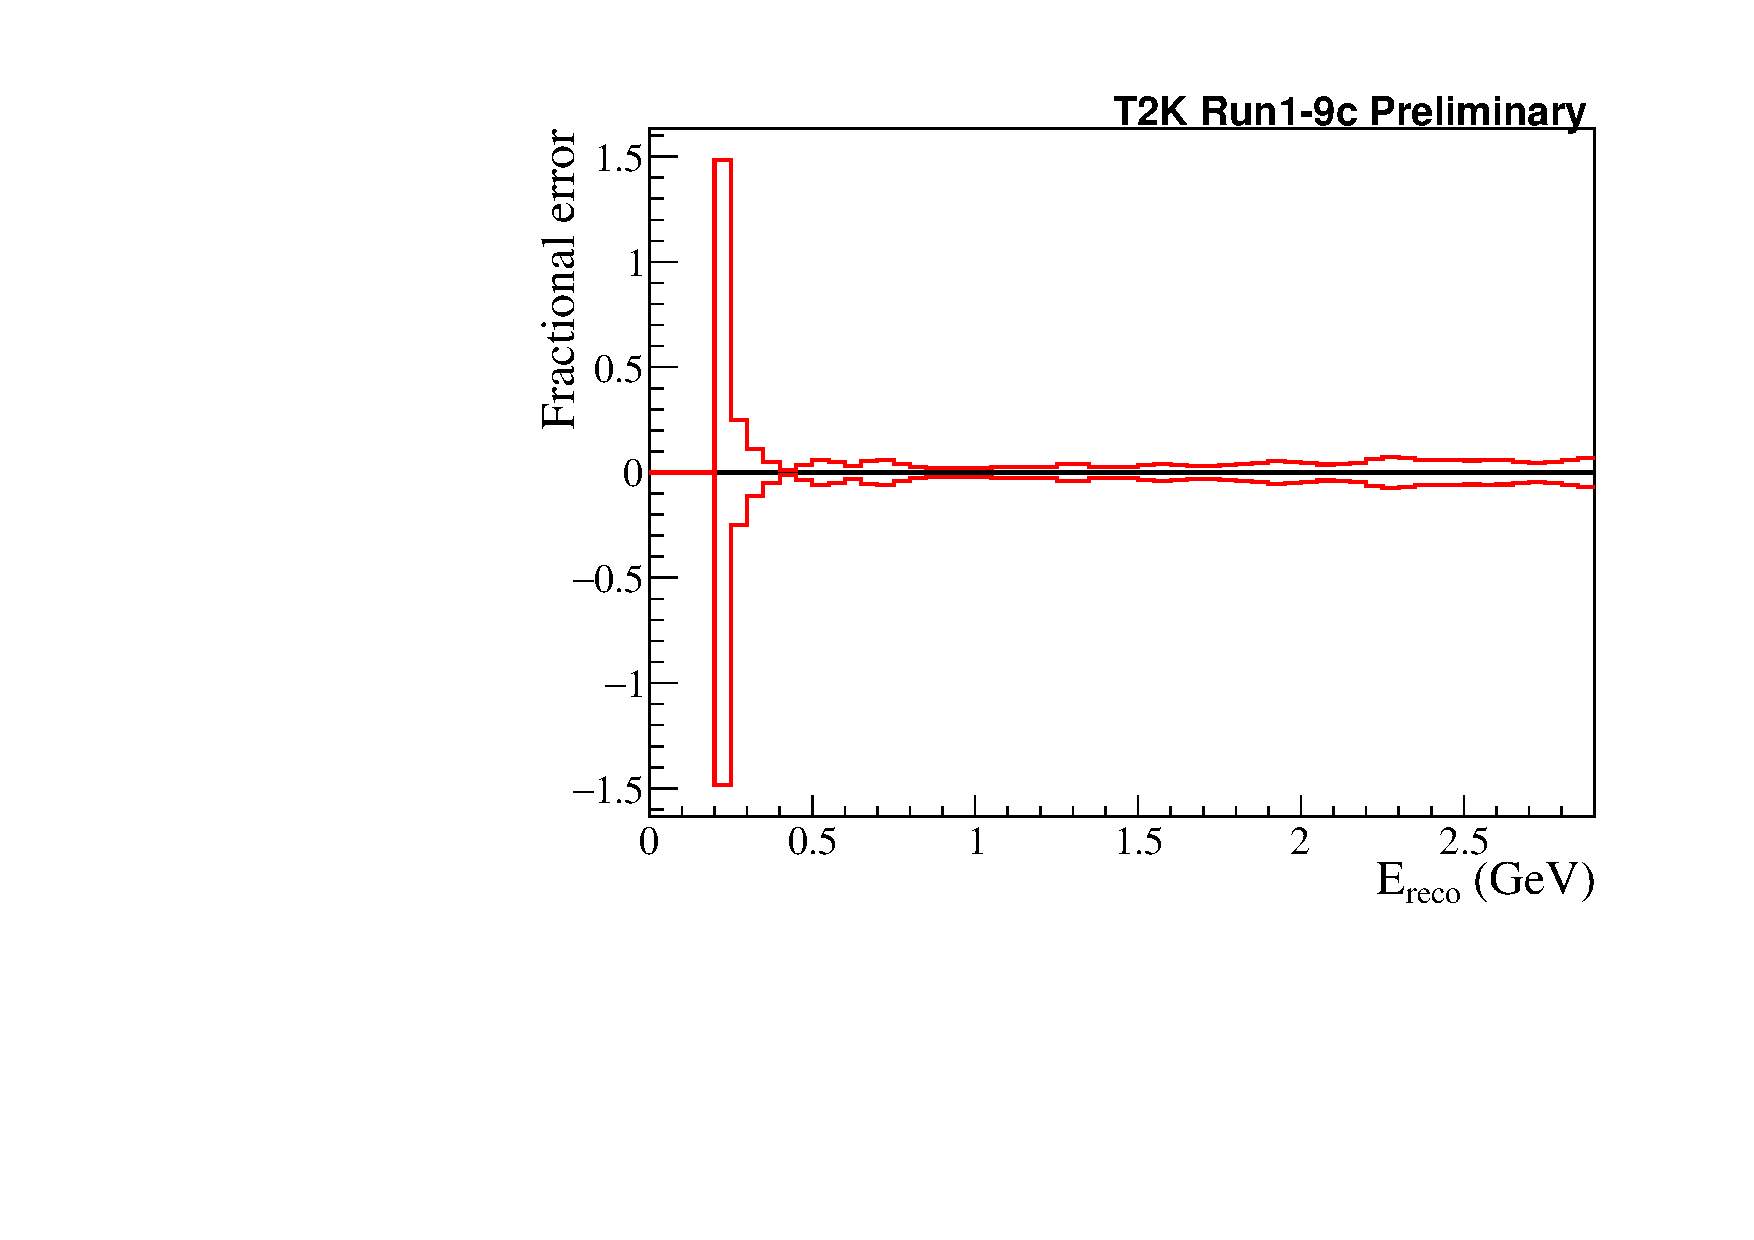
\includegraphics[width=0.9\textwidth]{images/systematics/envelopes/sk_error_table_1Rmu_skfsi_envelope_fractional}
		\caption{Muon-like, neutrino mode}
	\end{subfigure}
	\begin{subfigure}[b]{0.49\textwidth}
		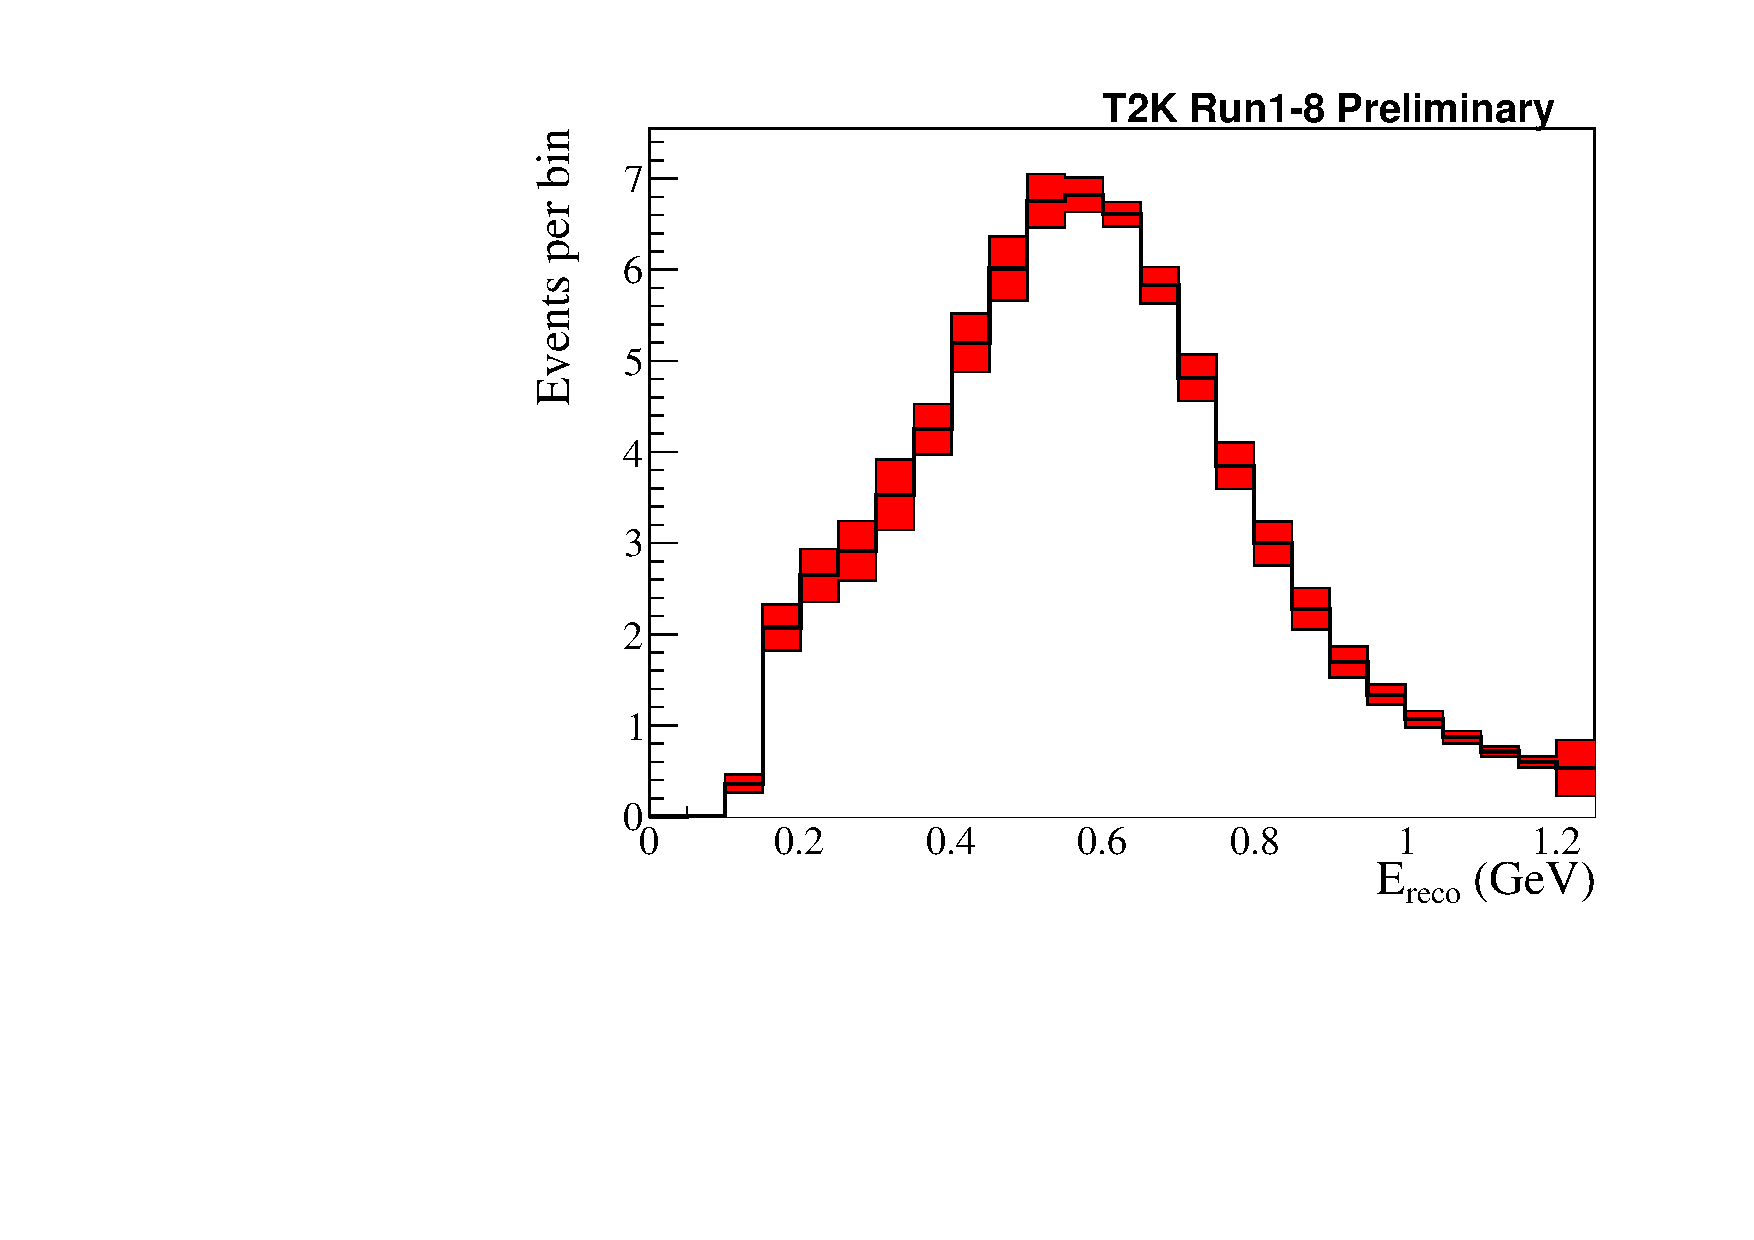
\includegraphics[width=0.9\textwidth]{images/systematics/envelopes/sk_error_table_1Re_skfsi_envelope}
		\caption{Electron-like, neutrino mode}
	\end{subfigure}
	\begin{subfigure}[b]{0.49\textwidth}
		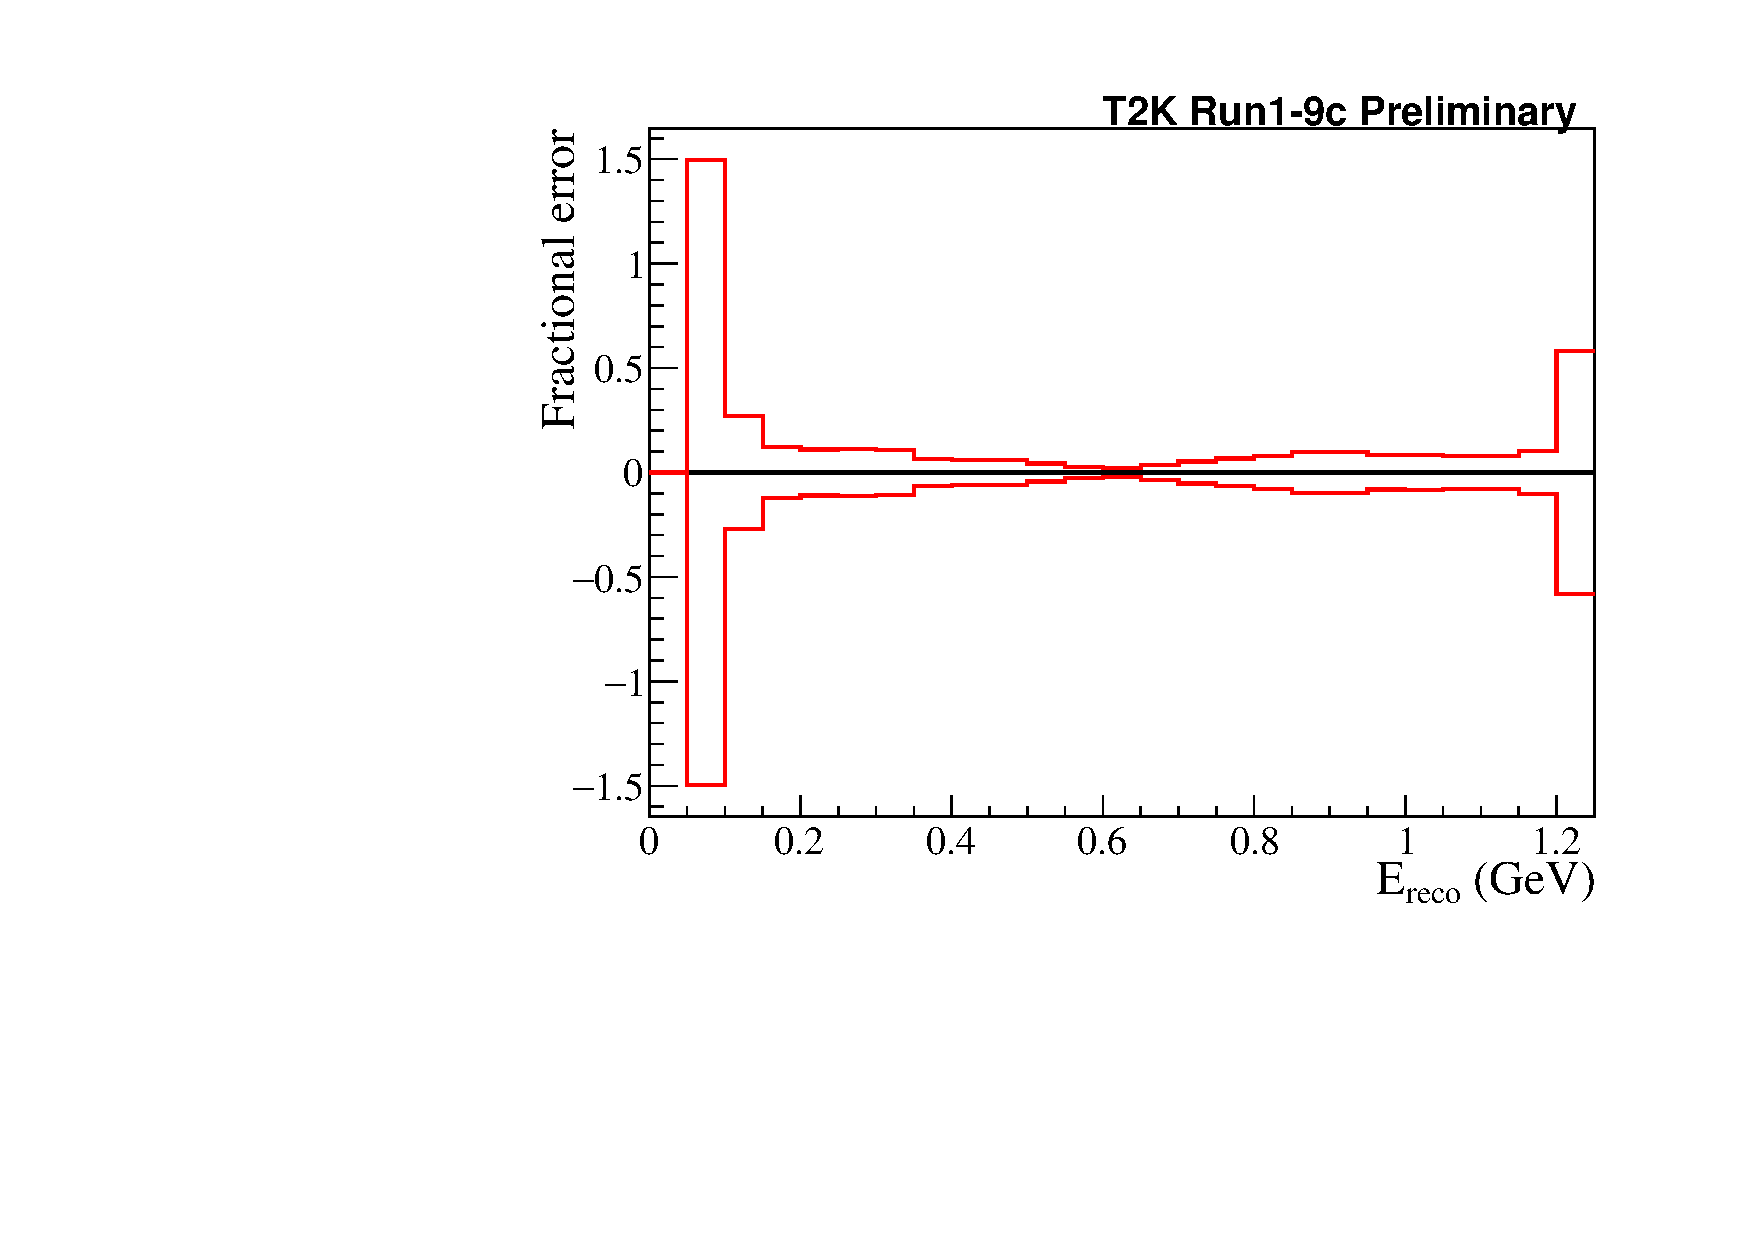
\includegraphics[width=0.9\textwidth]{images/systematics/envelopes/sk_error_table_1Re_skfsi_envelope_fractional}
		\caption{Electron-like, neutrino mode}
	\end{subfigure}
	\begin{subfigure}[b]{0.49\textwidth}
		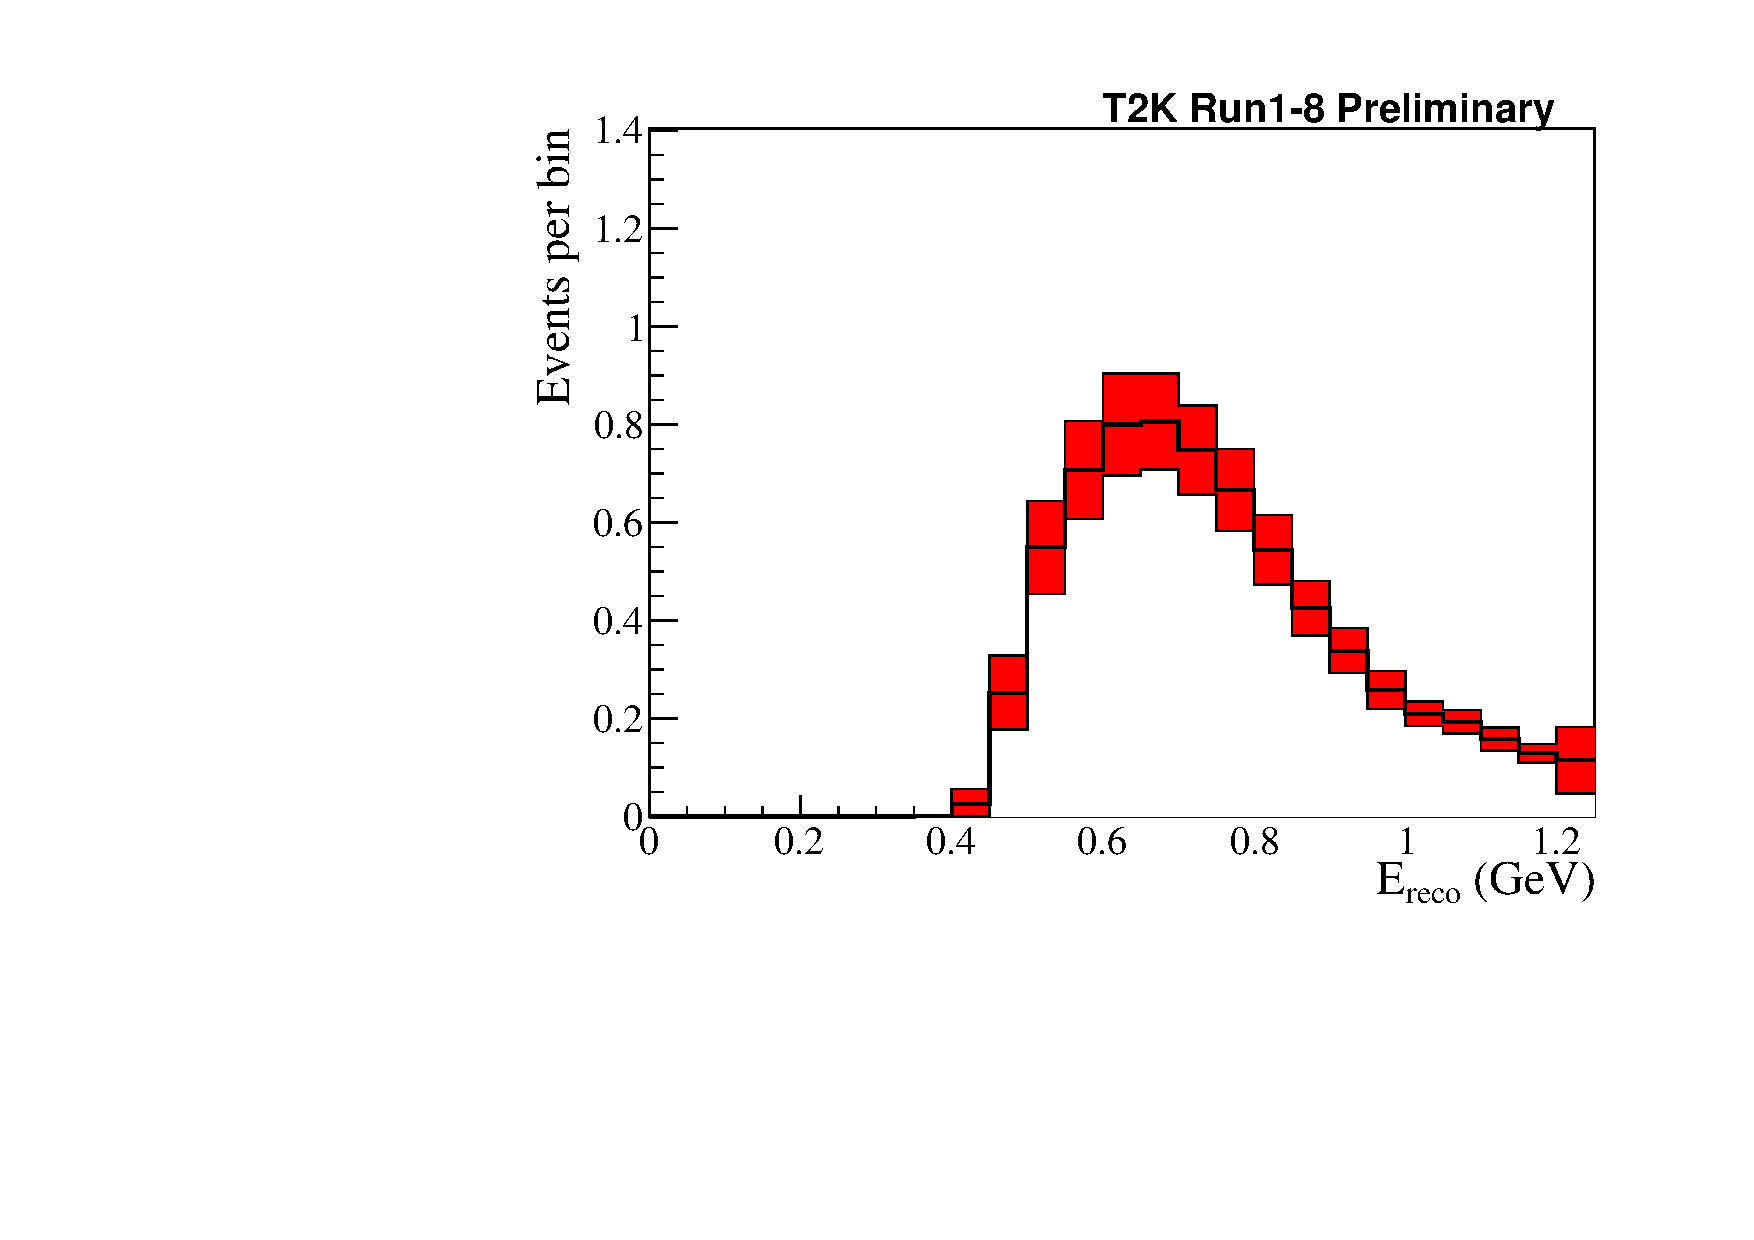
\includegraphics[width=0.9\textwidth]{images/systematics/envelopes/sk_error_table_MultiRe_skfsi_envelope}
		\caption{\nueCConepi-like, neutrino mode}
	\end{subfigure}
	\begin{subfigure}[b]{0.49\textwidth}
		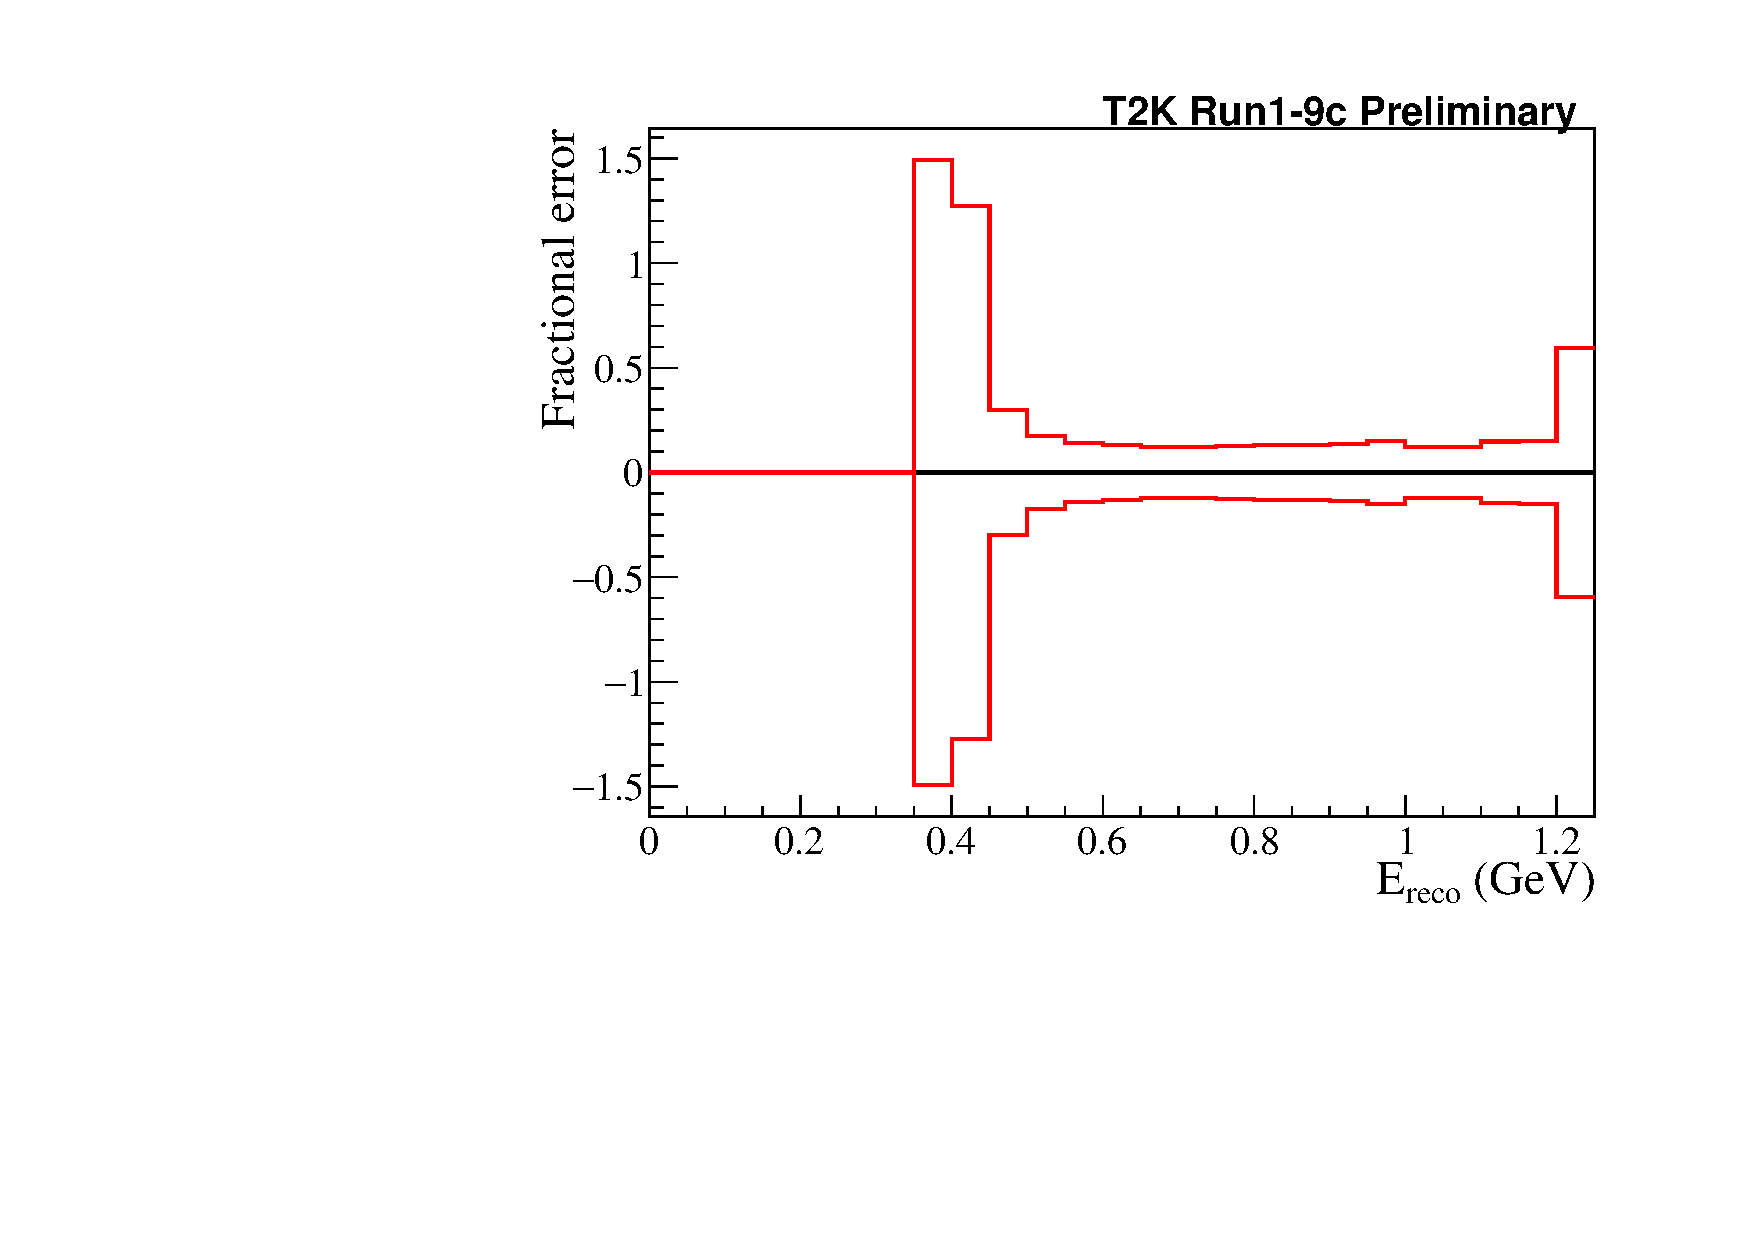
\includegraphics[width=0.9\textwidth]{images/systematics/envelopes/sk_error_table_MultiRe_skfsi_envelope_fractional}
		\caption{\nueCConepi-like, neutrino mode}
	\end{subfigure}
	\caption {
		Error envelopes (left) and fractional error (right) for the reconstructed neutrino energy spectrum for Super-K FSI+SI+PN systematic parameters. \NumToysSmall toys are generated for the Asimov data set A with randomized systematic parameters with correlations taken into account.
	}
	\label{fig:sk_envelopes_skfsi}
\end{figure*}
\clearpage

\begin{figure*}
	\center
	\begin{subfigure}[b]{0.49\textwidth}
		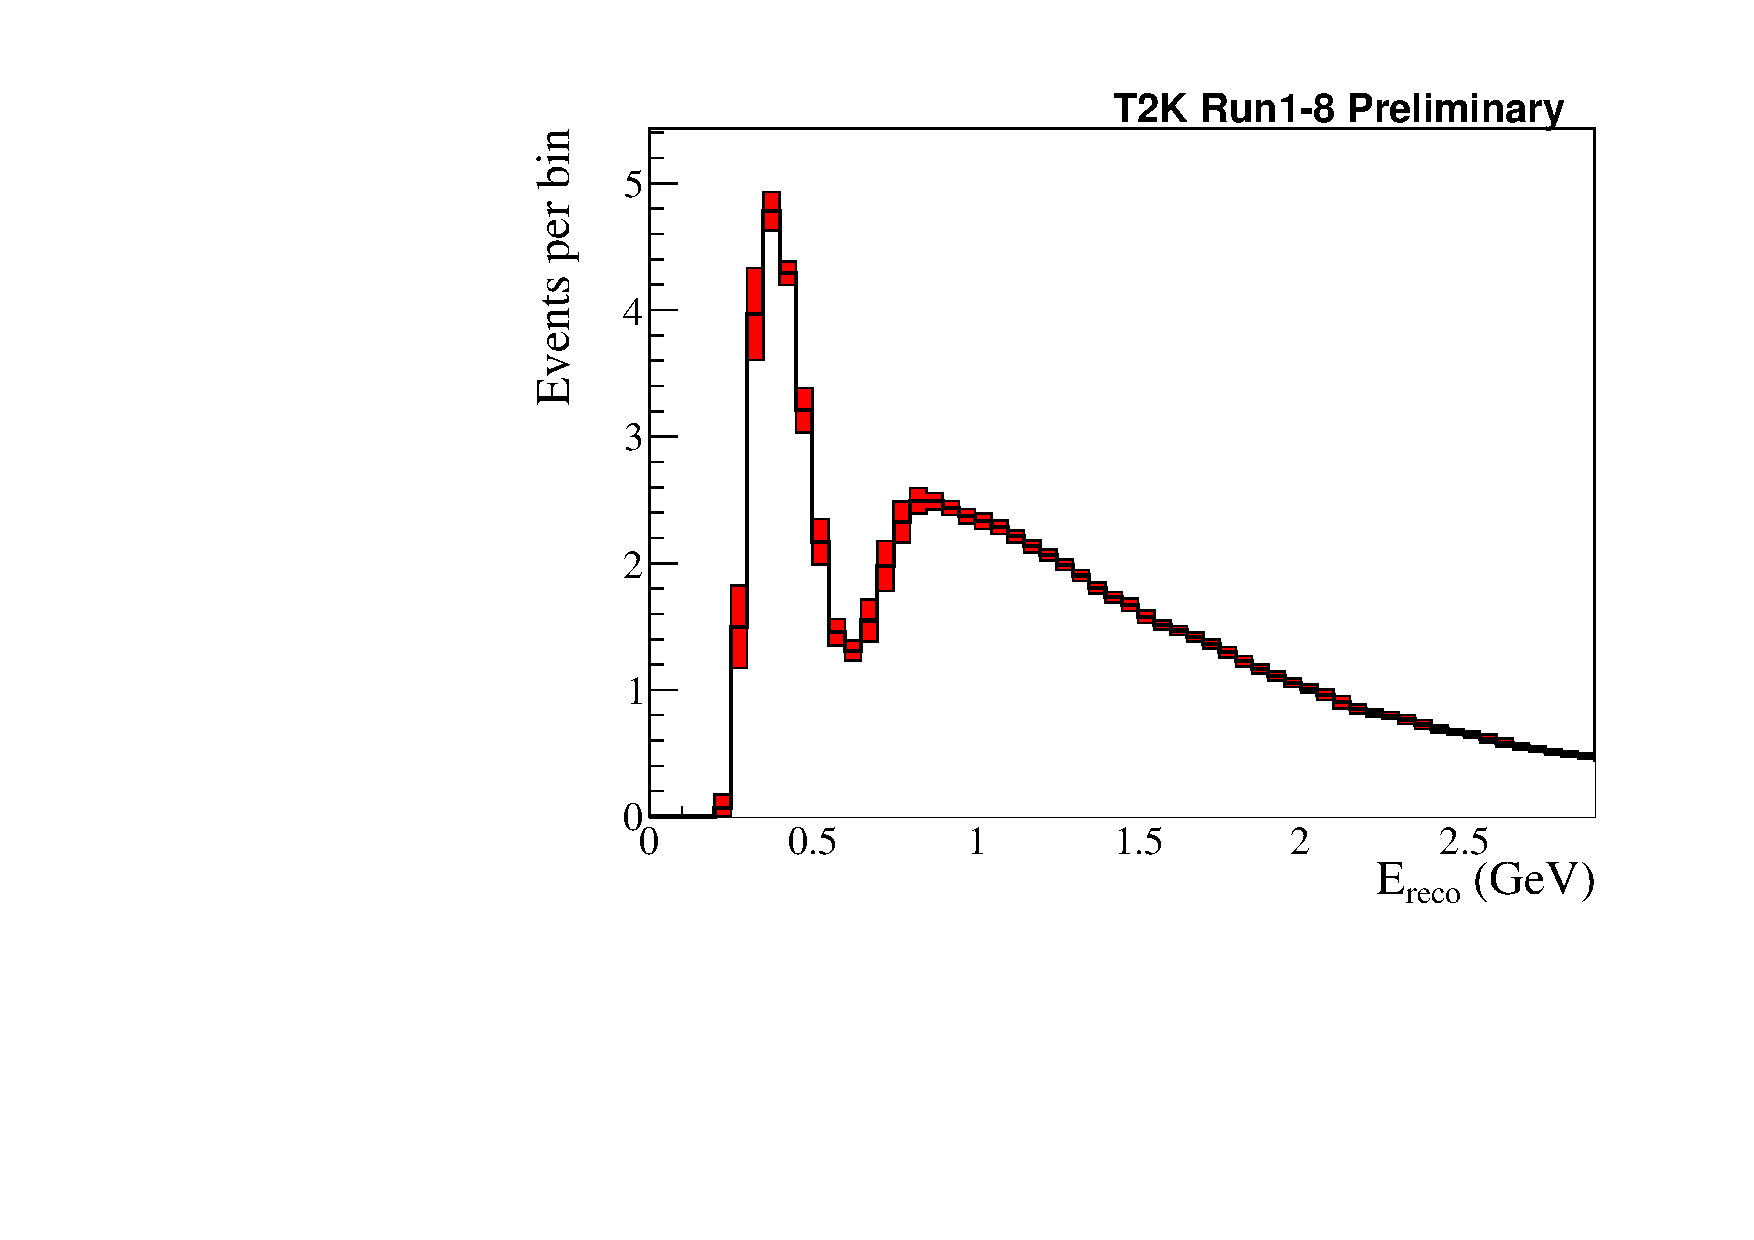
\includegraphics[width=0.9\textwidth]{images/systematics/envelopes/sk_error_table_RHC1Rmu_skfsi_envelope}
		\caption{Muon-like, antineutrino mode}
	\end{subfigure}
	\begin{subfigure}[b]{0.49\textwidth}
		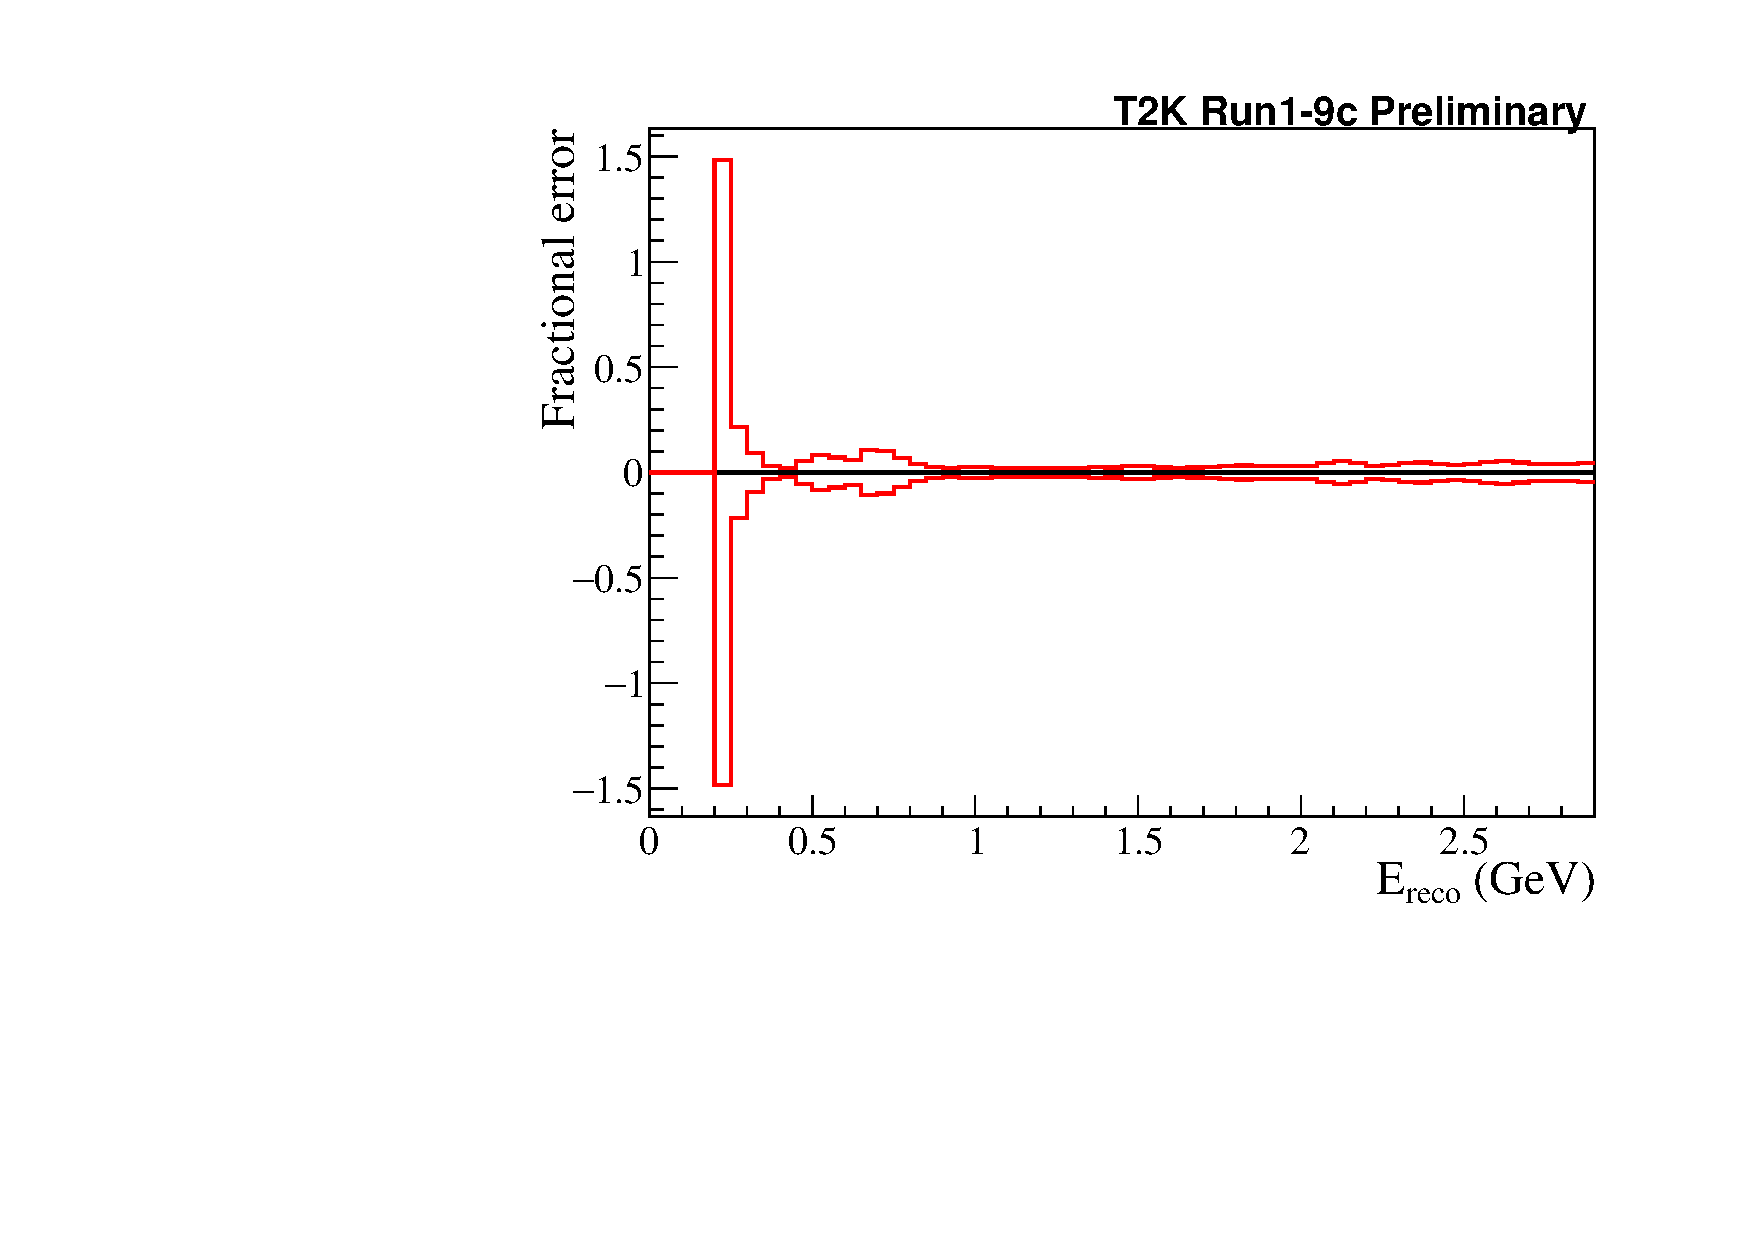
\includegraphics[width=0.9\textwidth]{images/systematics/envelopes/sk_error_table_RHC1Rmu_skfsi_envelope_fractional}
		\caption{Muon-like, antineutrino mode}
	\end{subfigure}
	\begin{subfigure}[b]{0.49\textwidth}
		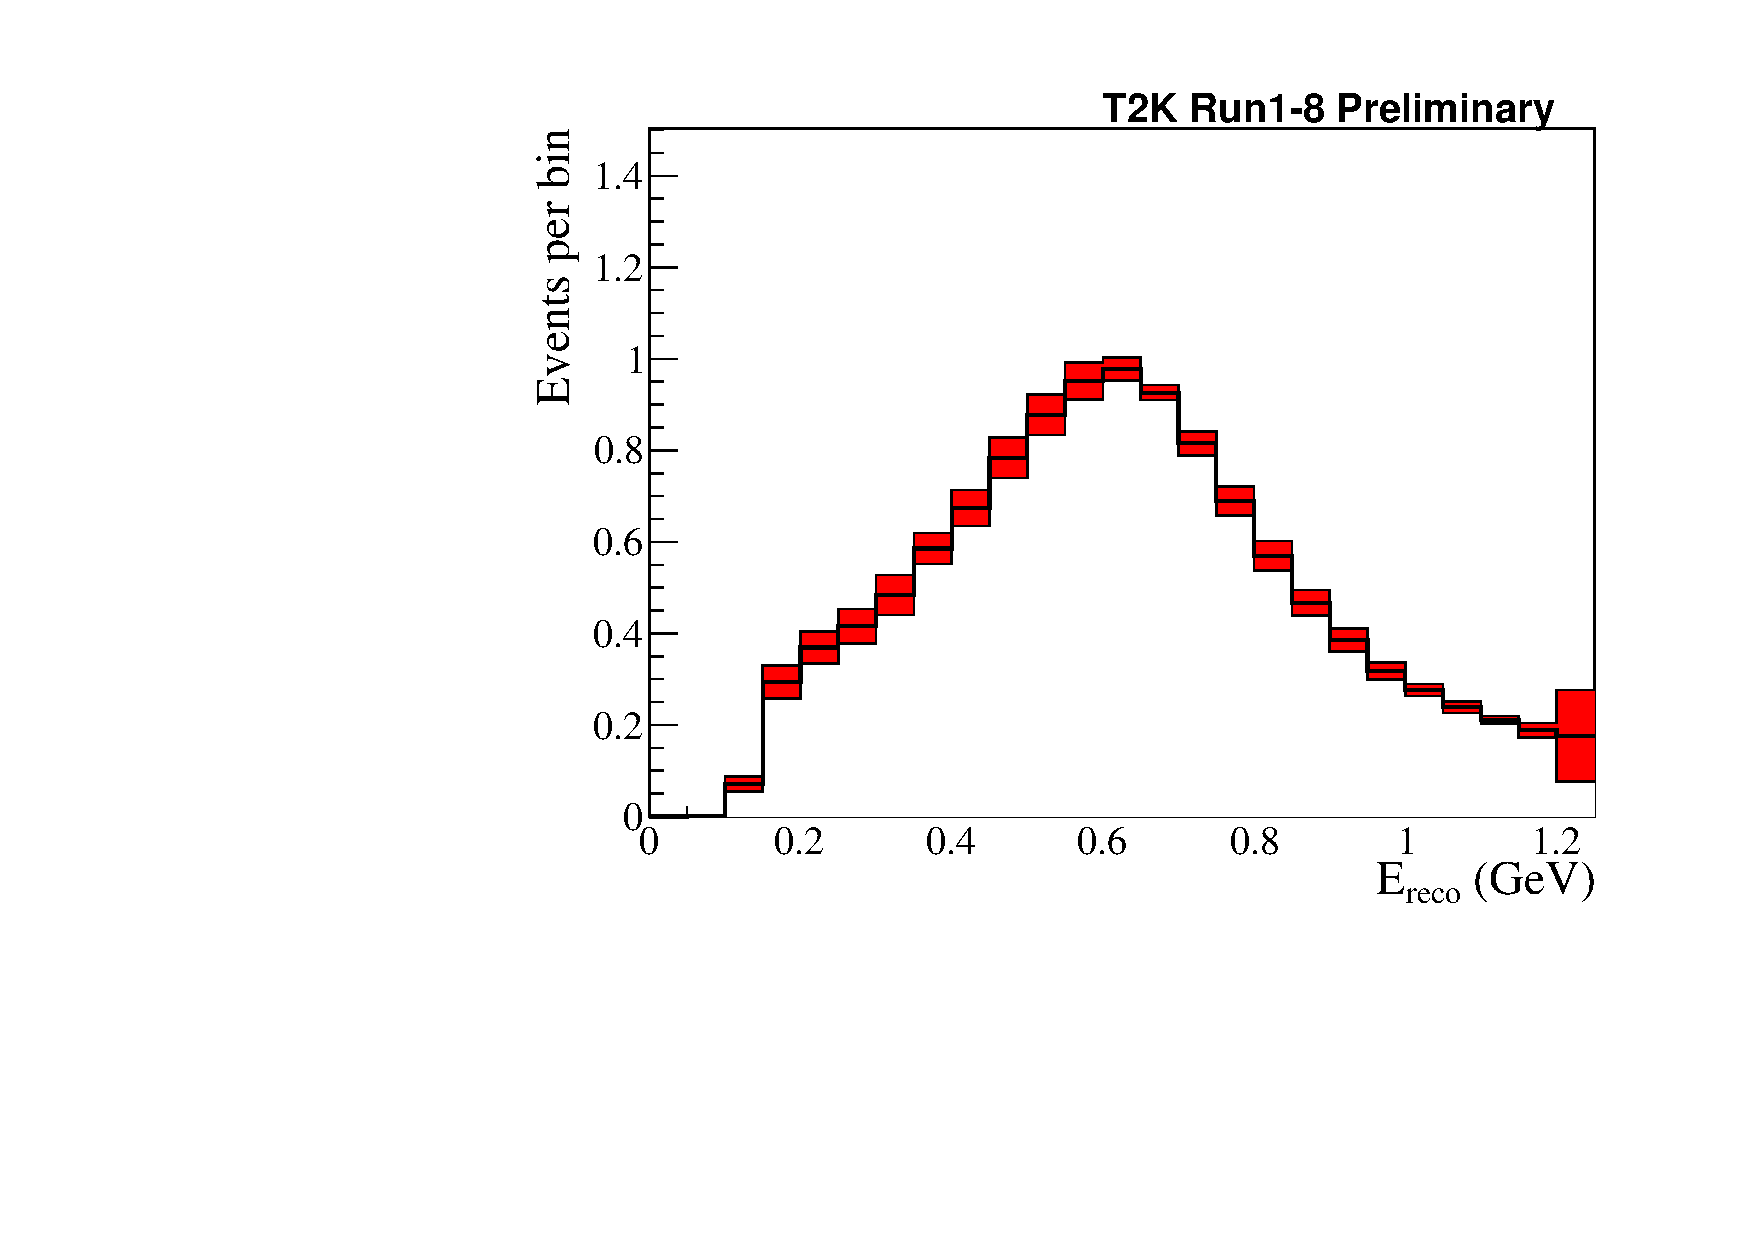
\includegraphics[width=0.9\textwidth]{images/systematics/envelopes/sk_error_table_RHC1Re_skfsi_envelope}
		\caption{Electron-like antineutrino mode}
	\end{subfigure}
	\begin{subfigure}[b]{0.49\textwidth}
		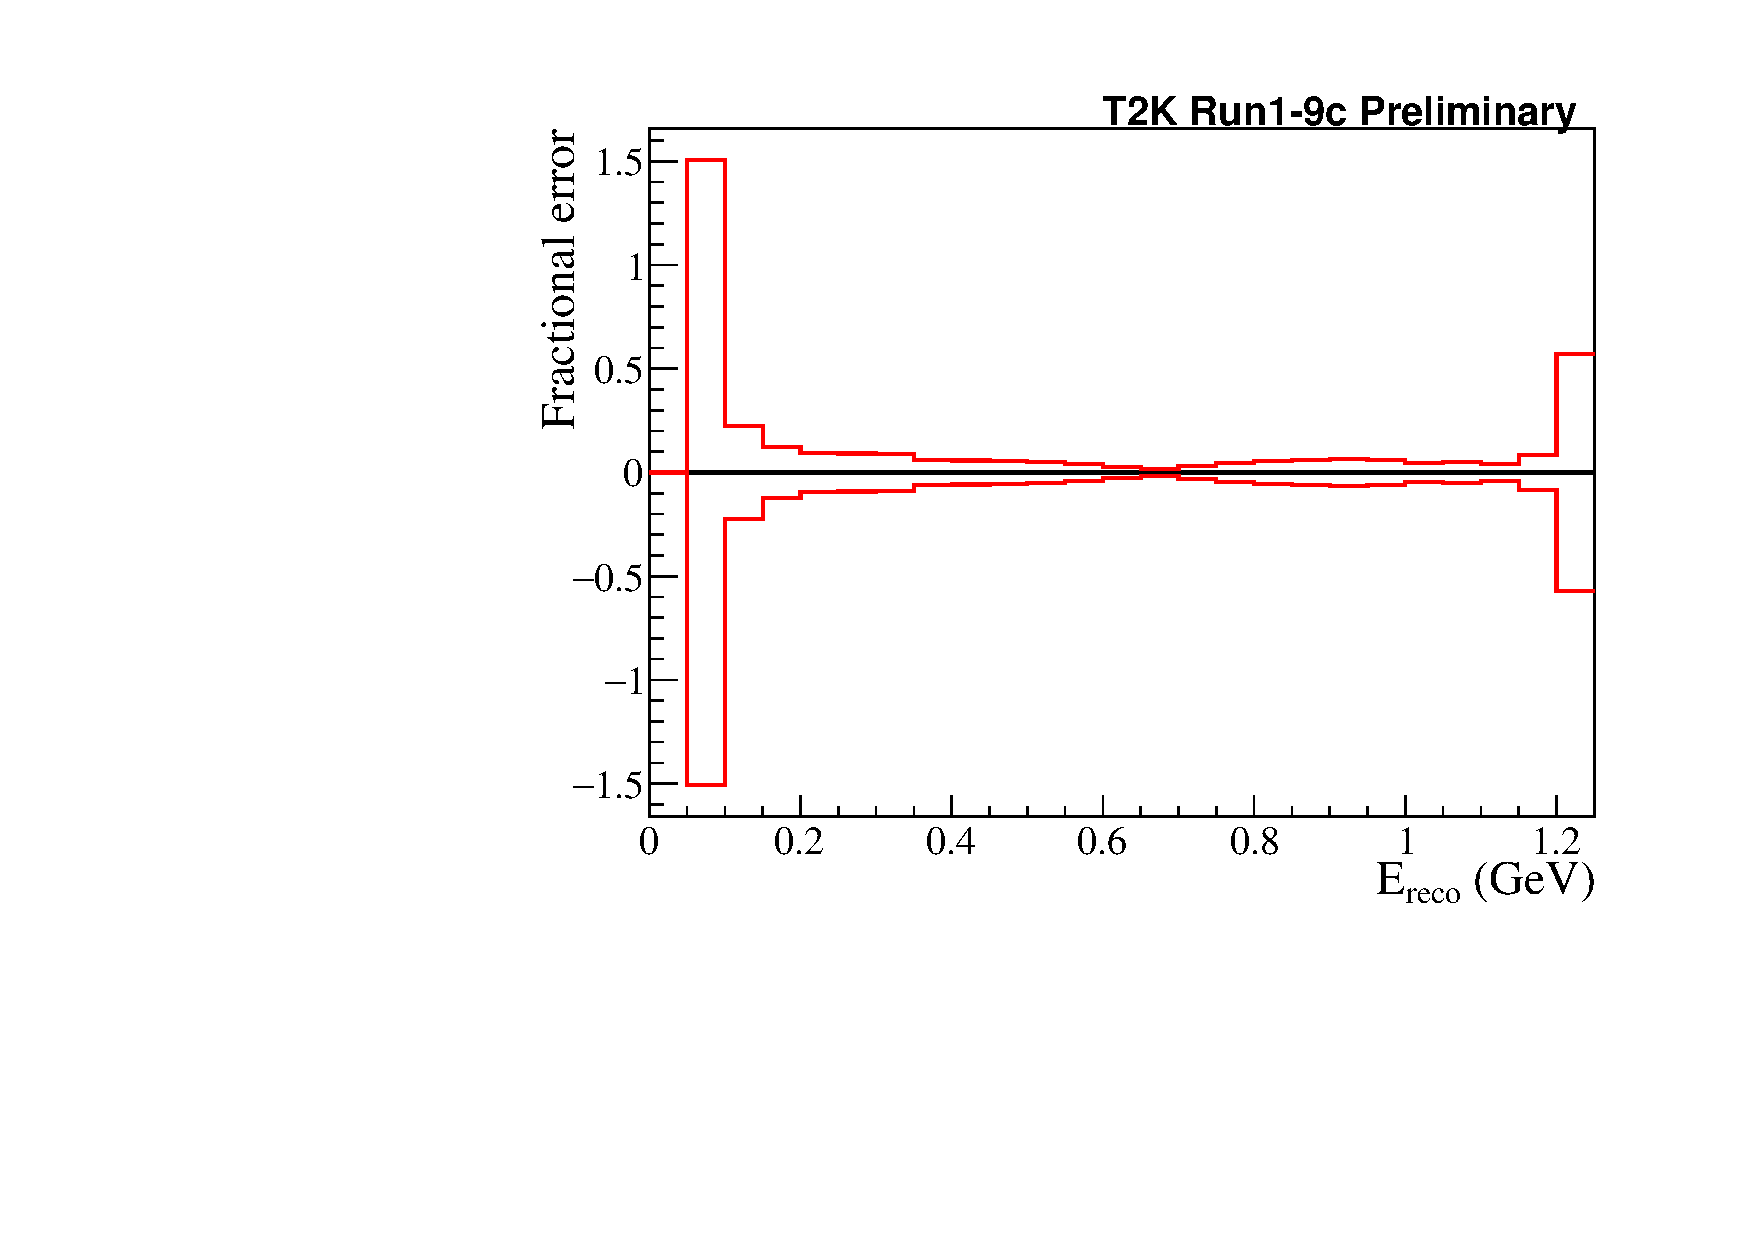
\includegraphics[width=0.9\textwidth]{images/systematics/envelopes/sk_error_table_RHC1Re_skfsi_envelope_fractional}
		\caption{Electron-like antineutrino mode}
	\end{subfigure}
	\caption {
		Error envelopes (left) and fractional errors (right) for the reconstructed neutrino energy spectrum for Super-K FSI+SI+PN systematic parameters. \NumToysSmall toys are generated for the Asimov data set A with randomized systematic parameters with correlations taken into account.
	}
	\label{fig:sk_envelopes_skfsi_b}
\end{figure*}
\clearpage
\begin{figure*}
	\center
	\begin{subfigure}[b]{0.49\textwidth}
		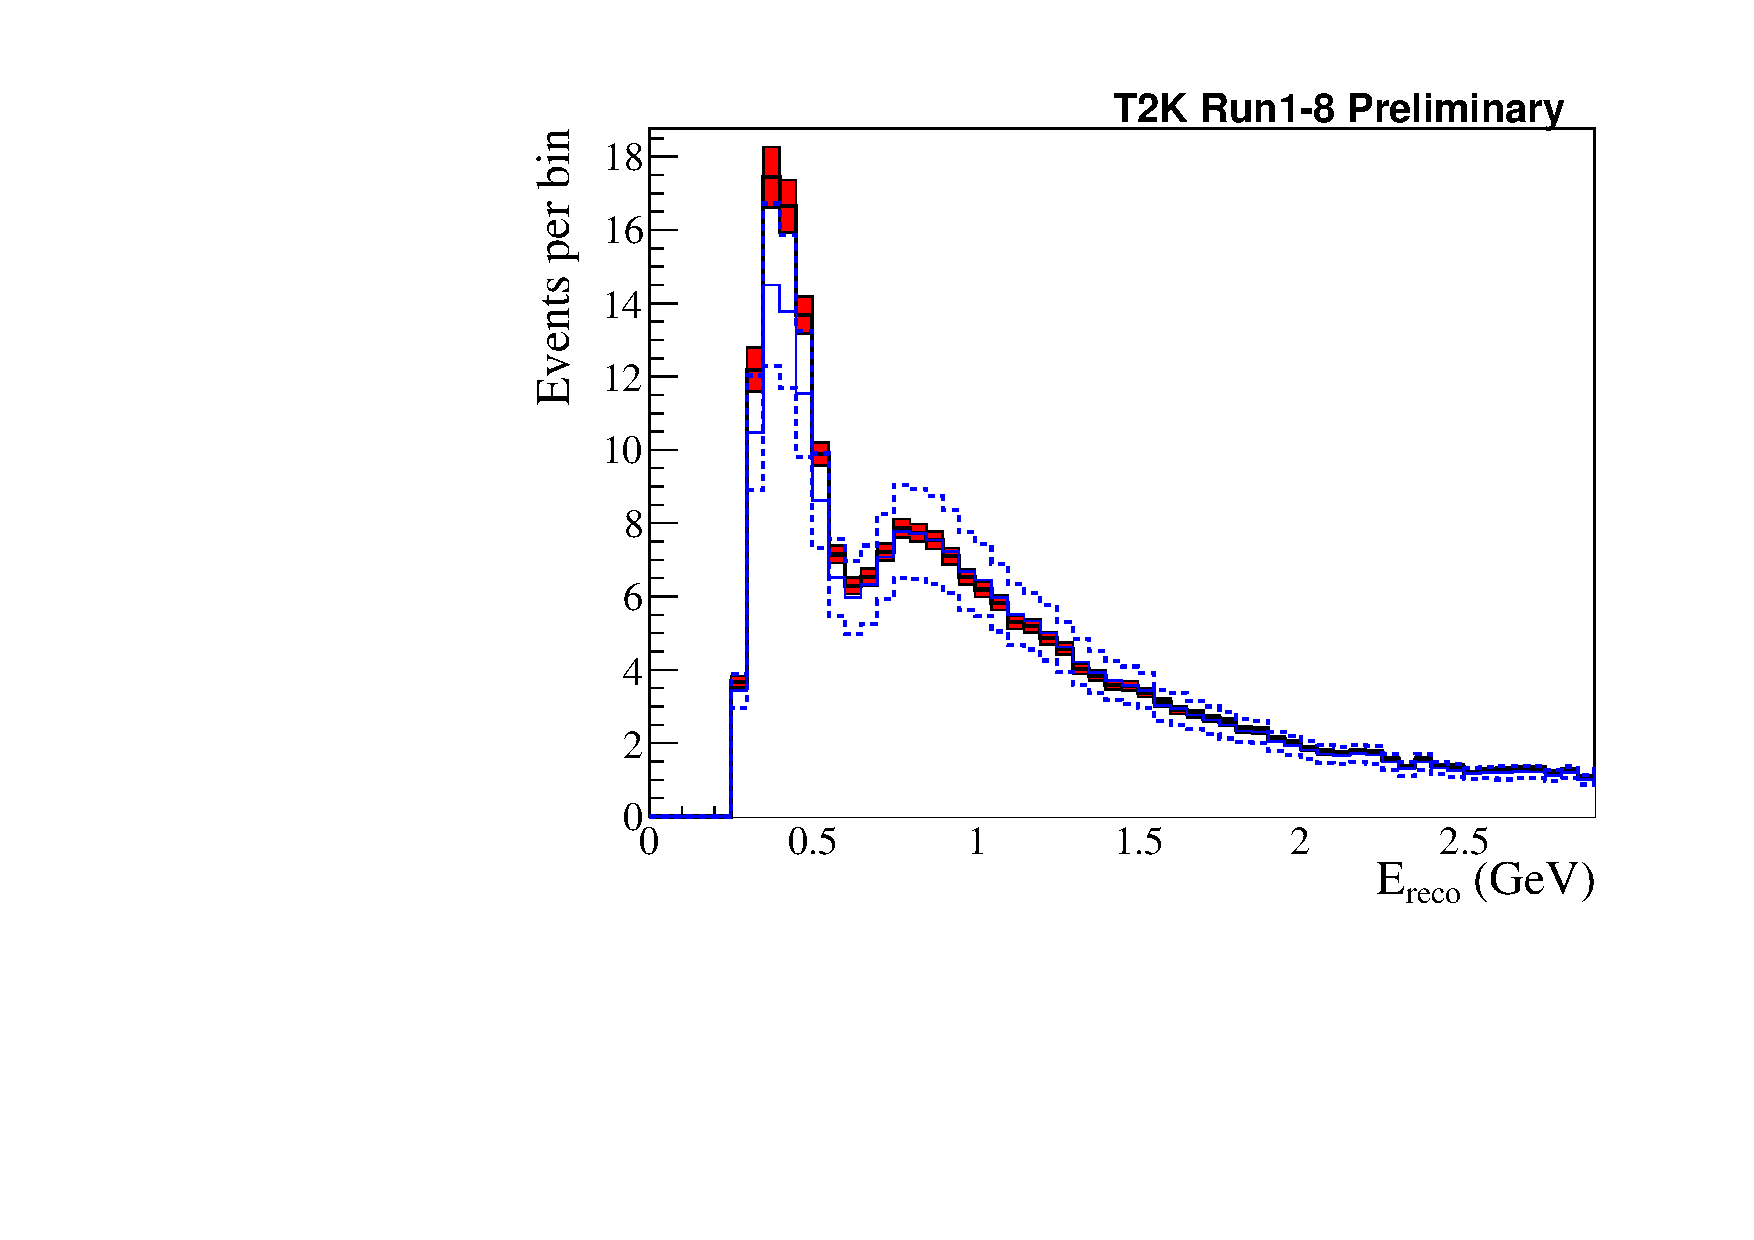
\includegraphics[width=0.9\textwidth]{images/systematics/envelopes/sk_error_table_1Rmu_banff_constrained_envelope}
		\caption{Muon-like, neutrino mode}
	\end{subfigure}
	\begin{subfigure}[b]{0.49\textwidth}
		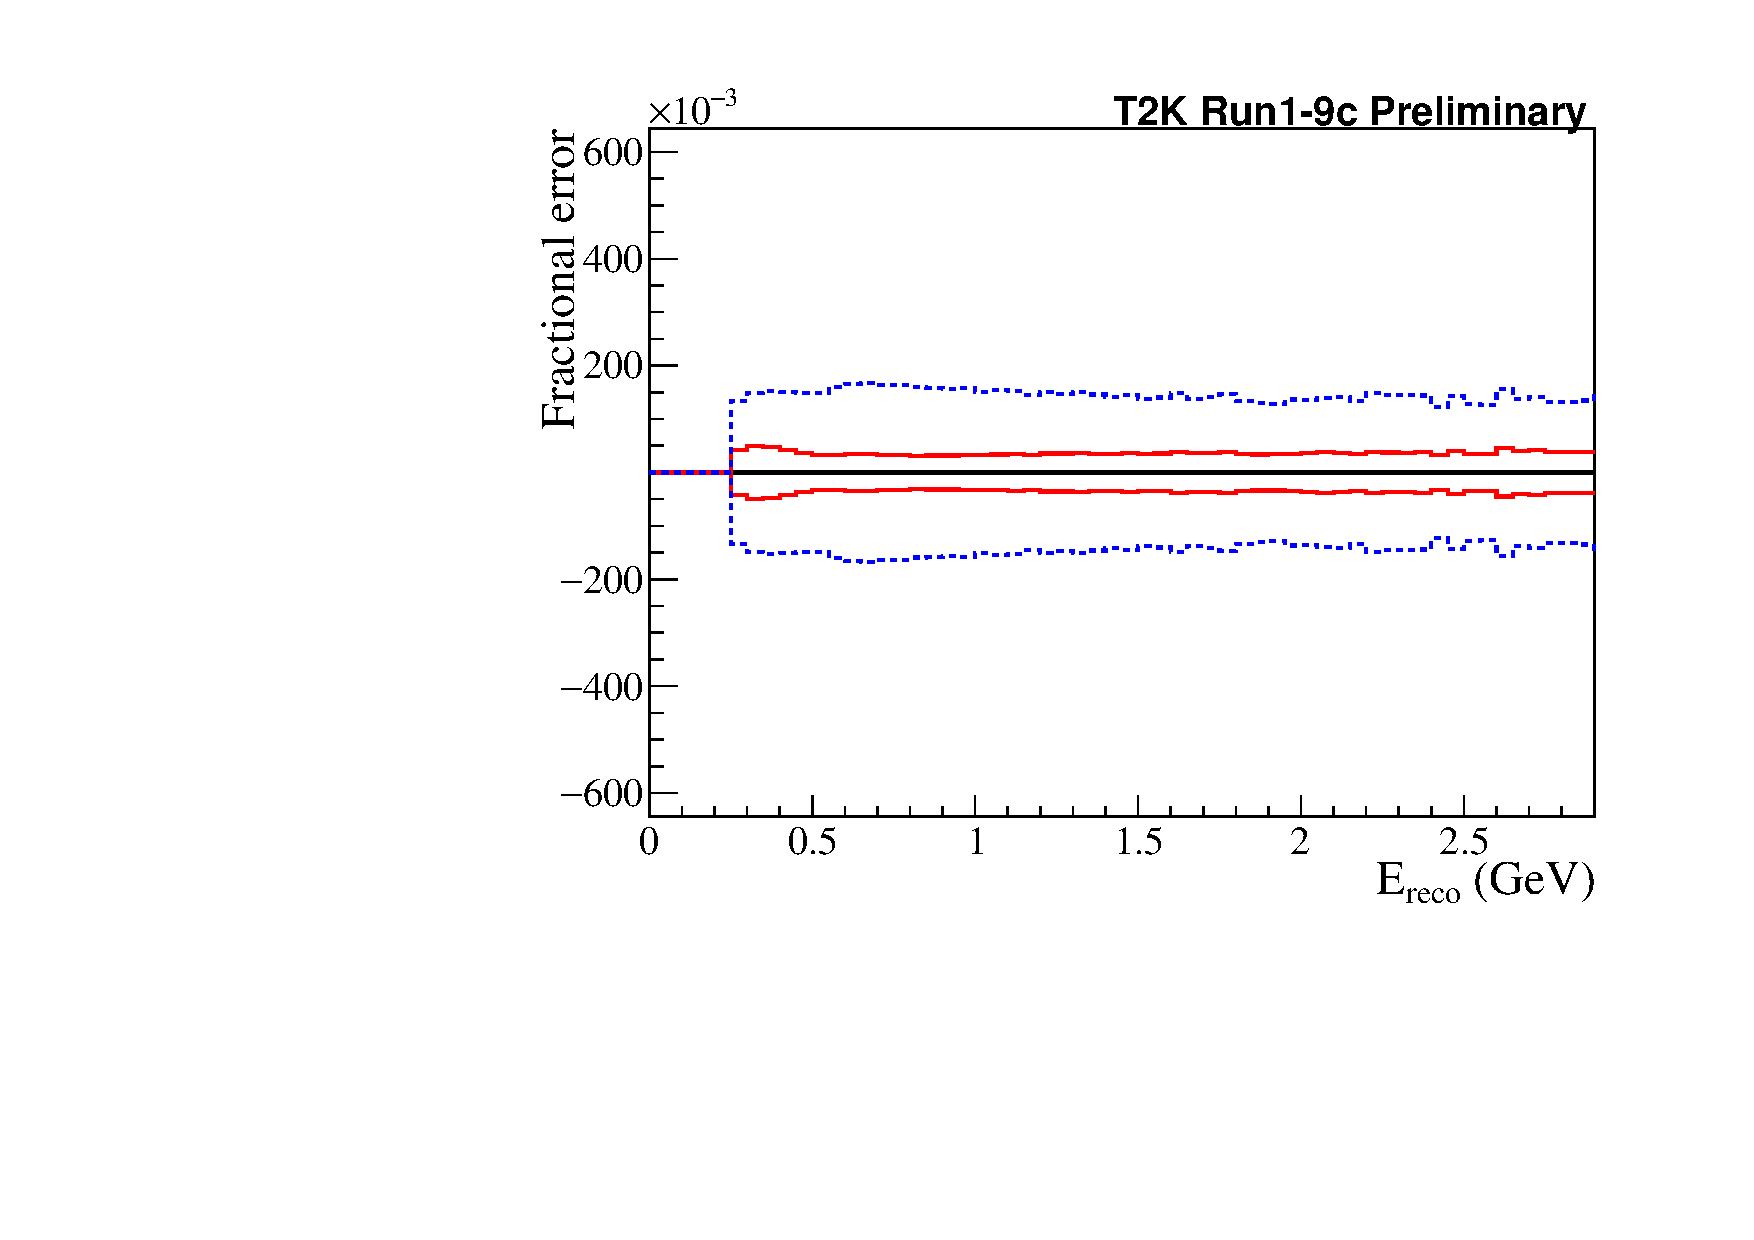
\includegraphics[width=0.9\textwidth]{images/systematics/envelopes/sk_error_table_1Rmu_banff_constrained_envelope_fractional}
		\caption{Muon-like, neutrino mode}
	\end{subfigure}
	\begin{subfigure}[b]{0.49\textwidth}
		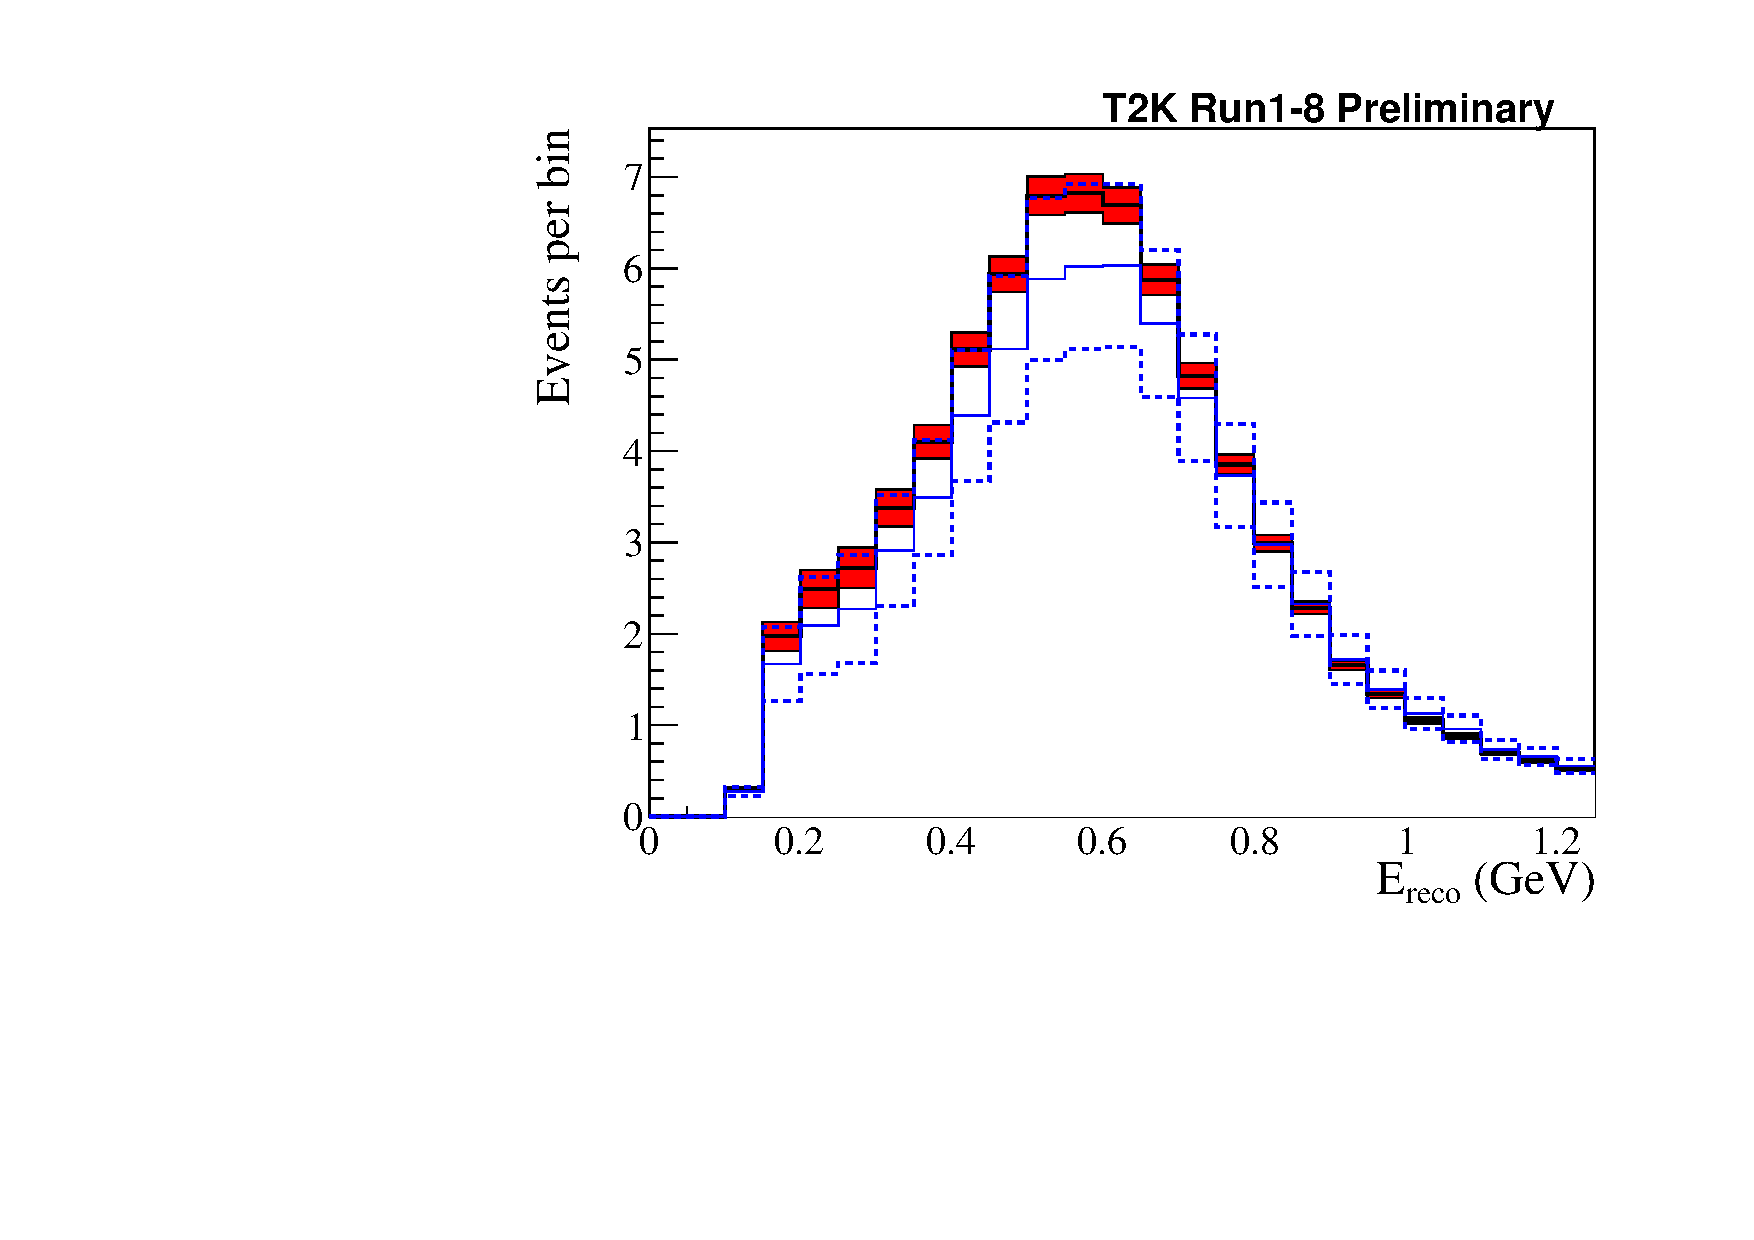
\includegraphics[width=0.9\textwidth]{images/systematics/envelopes/sk_error_table_1Re_banff_constrained_envelope}
		\caption{Electron-like, neutrino mode}
	\end{subfigure}
	\begin{subfigure}[b]{0.49\textwidth}
		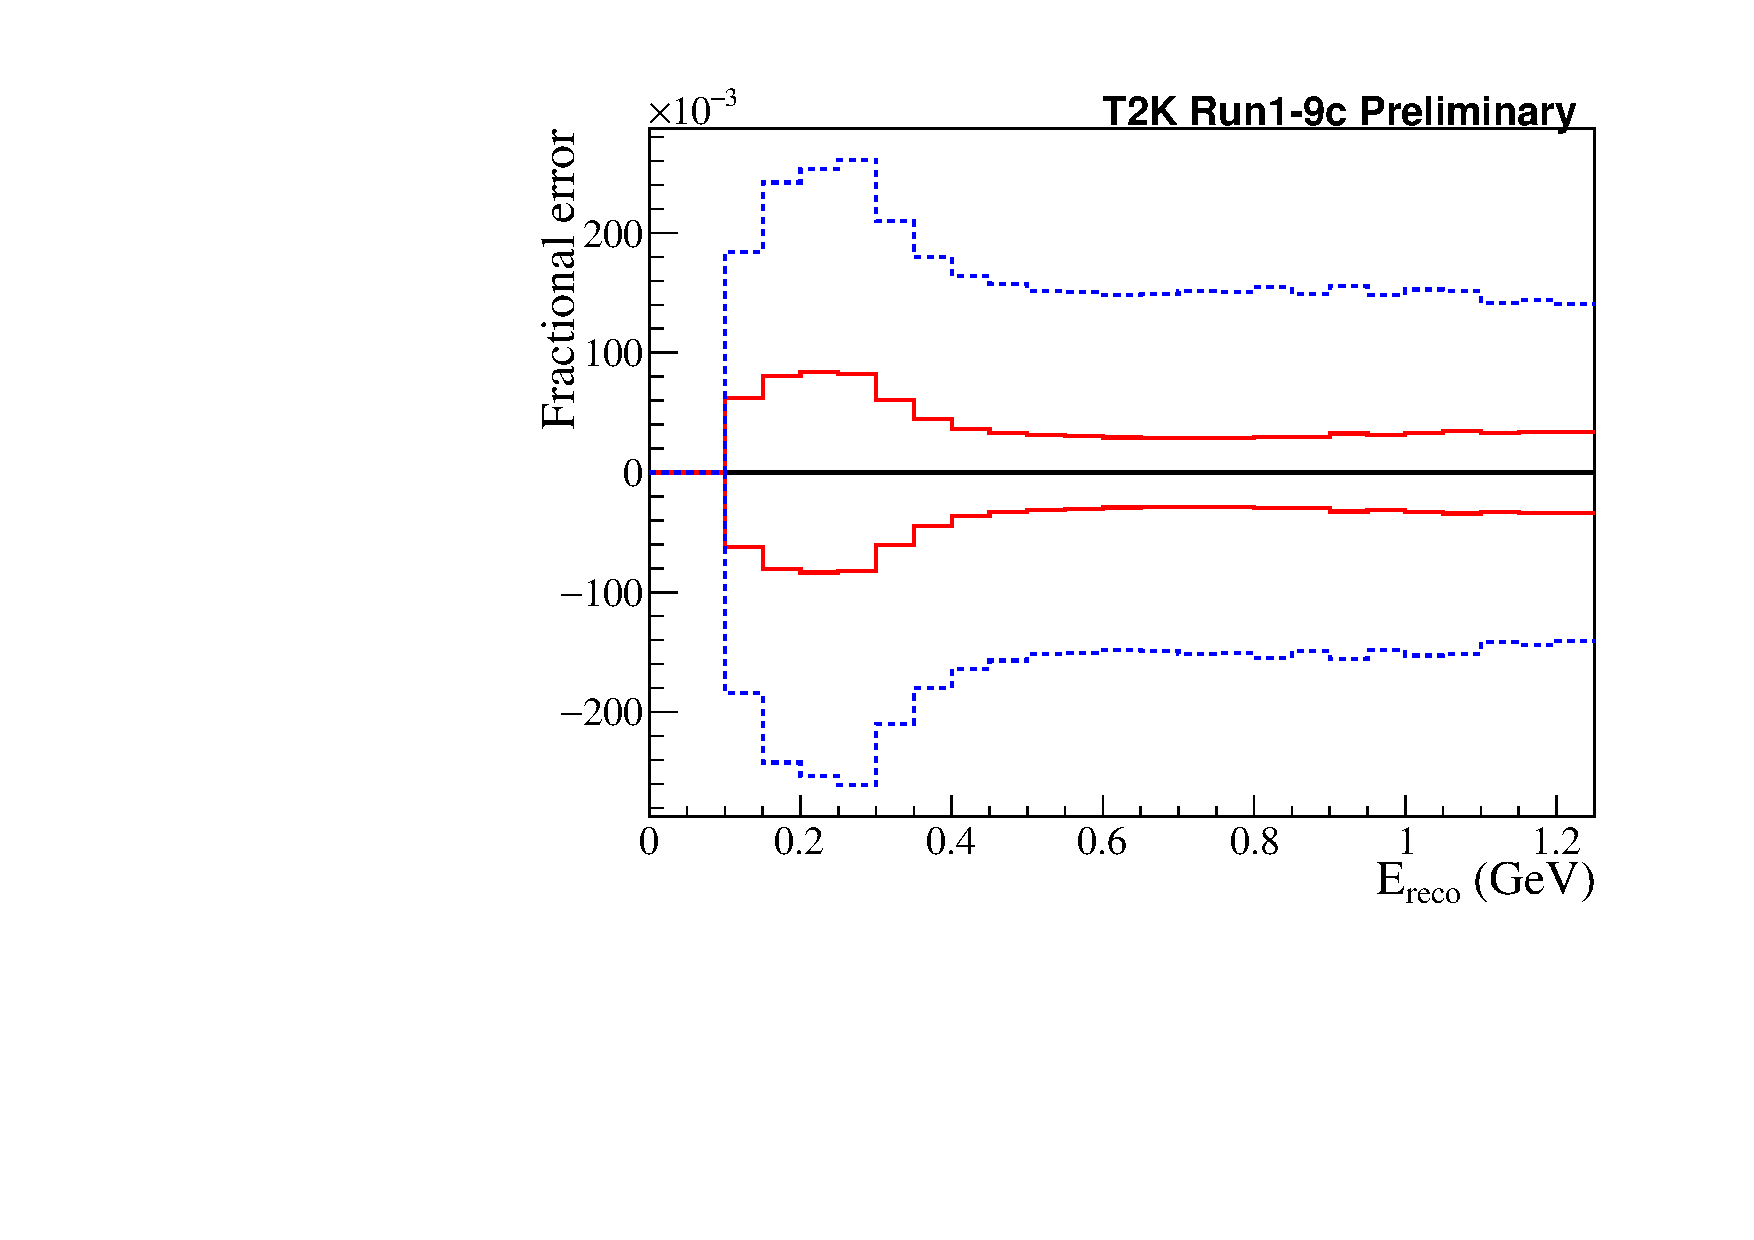
\includegraphics[width=0.9\textwidth]{images/systematics/envelopes/sk_error_table_1Re_banff_constrained_envelope_fractional}
		\caption{Electron-like, neutrino mode}
	\end{subfigure}
	\begin{subfigure}[b]{0.49\textwidth}
		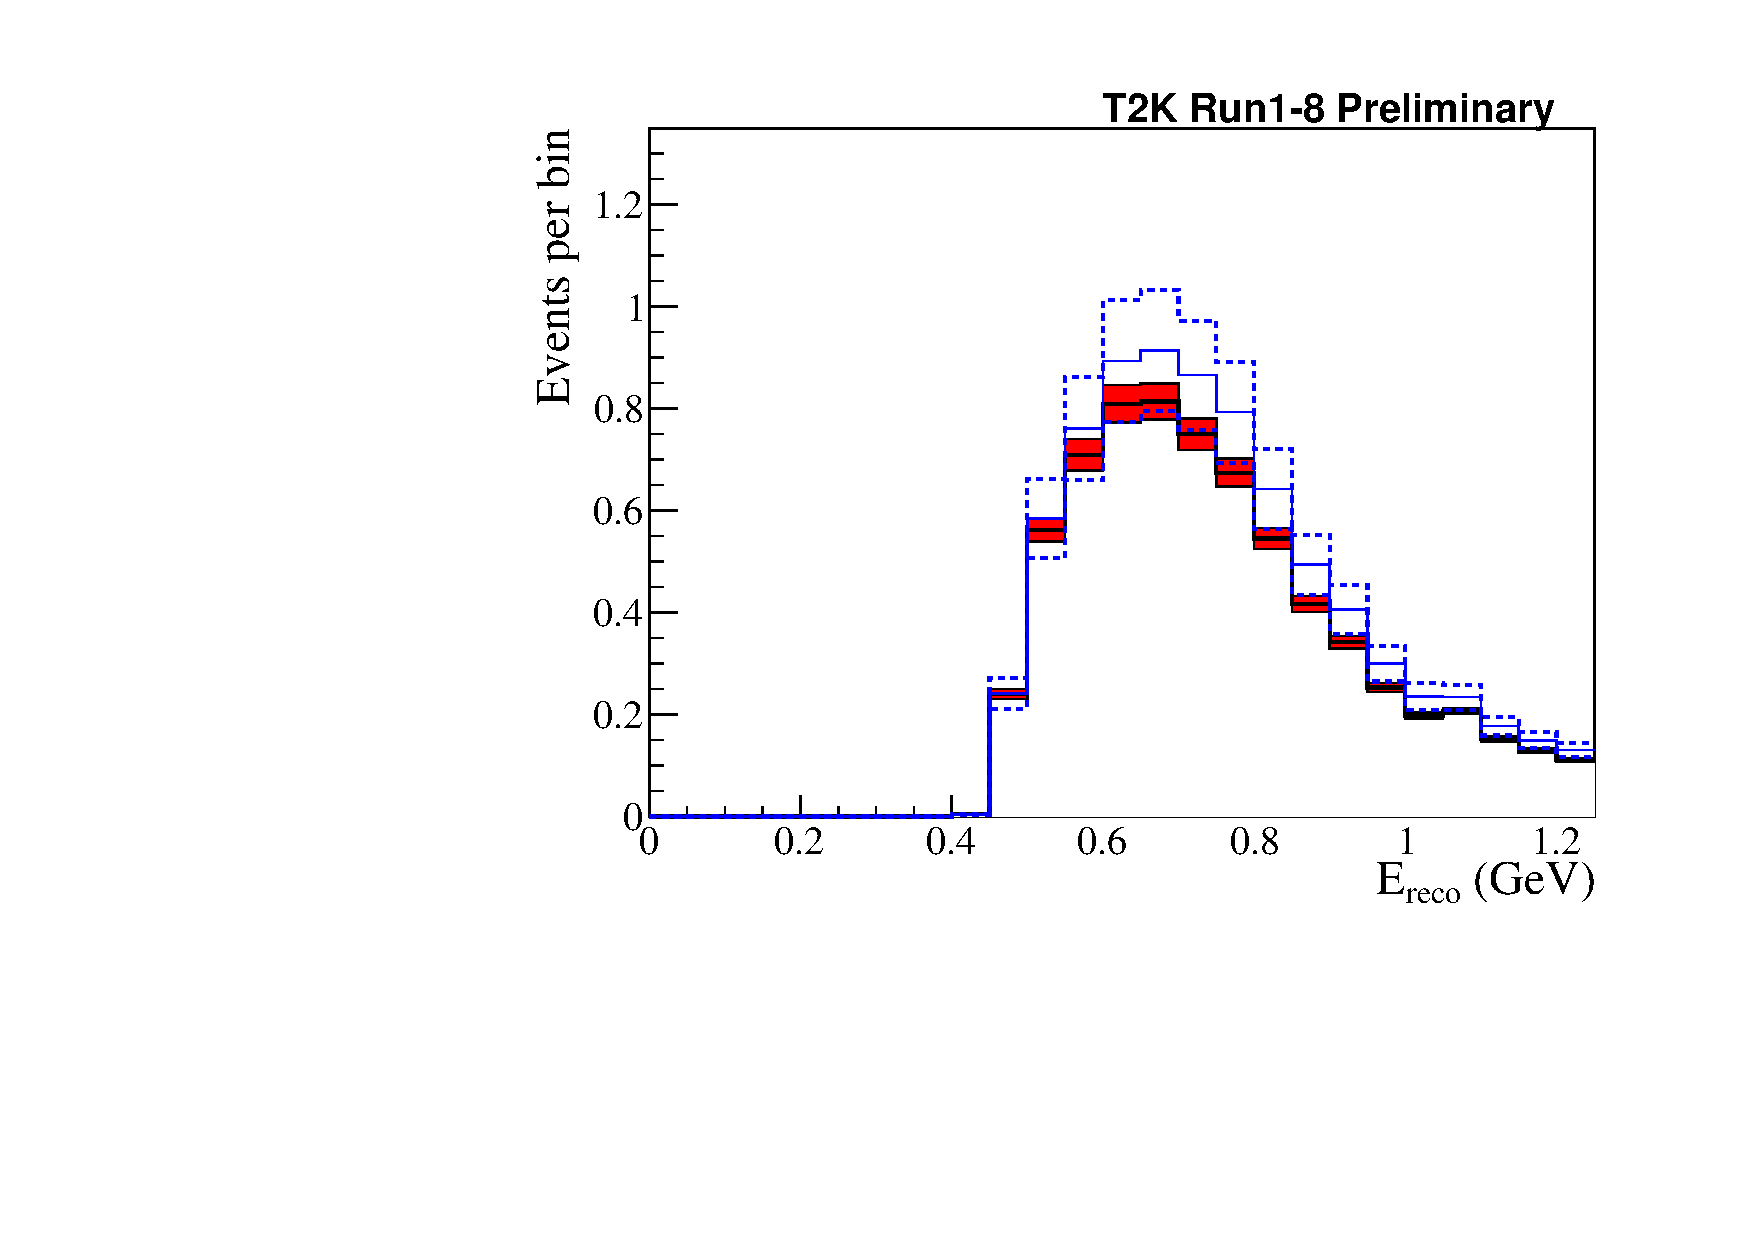
\includegraphics[width=0.9\textwidth]{images/systematics/envelopes/sk_error_table_MultiRe_banff_constrained_envelope}
		\caption{\nueCConepi-like, neutrino mode}
	\end{subfigure}
	\begin{subfigure}[b]{0.49\textwidth}
		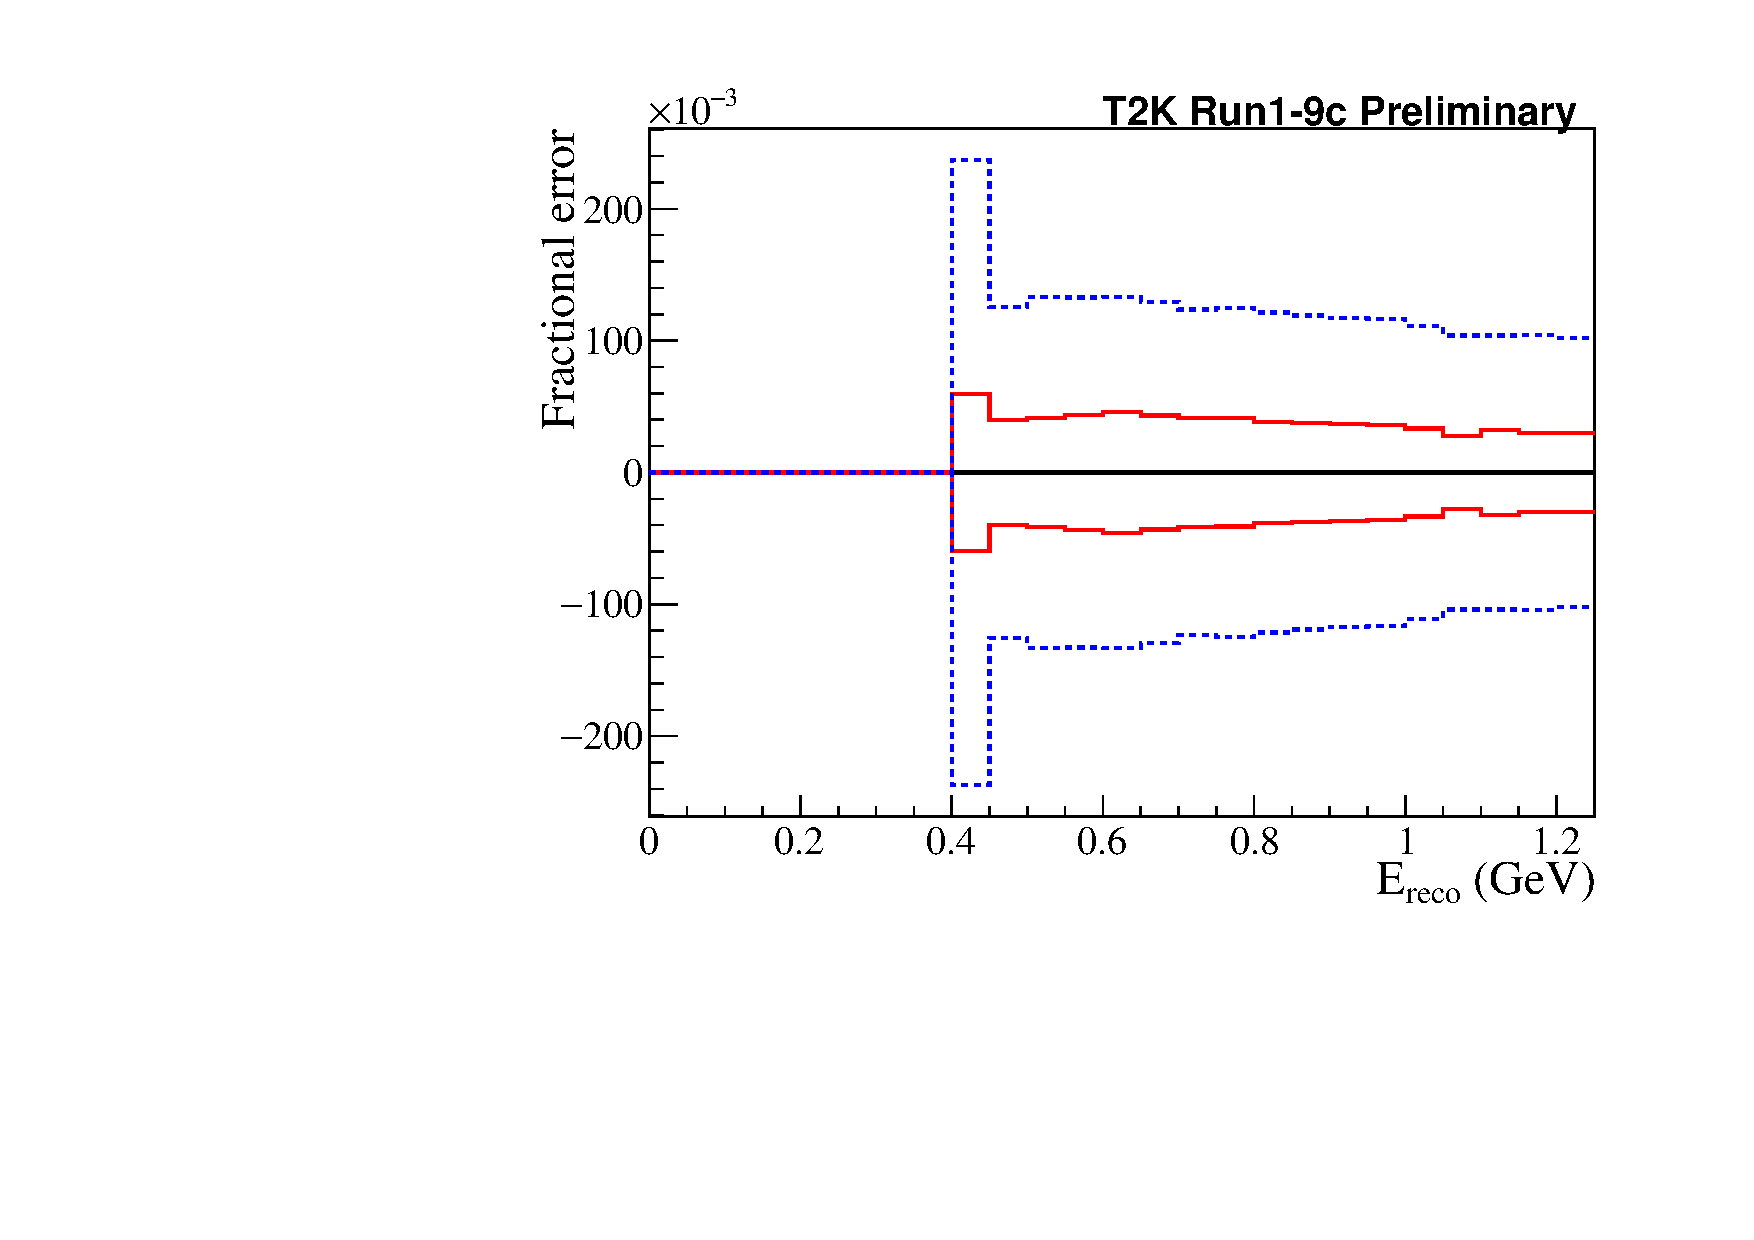
\includegraphics[width=0.9\textwidth]{images/systematics/envelopes/sk_error_table_MultiRe_banff_constrained_envelope_fractional}
		\caption{\nueCConepi-like, neutrino mode}
	\end{subfigure}
	\caption {
		Error envelopes (left) and fractional errors (right) for the reconstructed neutrino energy spectrum for the flux and constrained cross-section systematic parameters for pre-BANFF (blue) and post-BANFF (red) errors. \NumToysSmall toys are generated for the Asimov data set A with randomized systematic parameters with correlations taken into account.
	}
	\label{fig:sk_envelopes_banff}
\end{figure*}
\clearpage

\begin{figure*}
	\center
	\begin{subfigure}[b]{0.49\textwidth}
		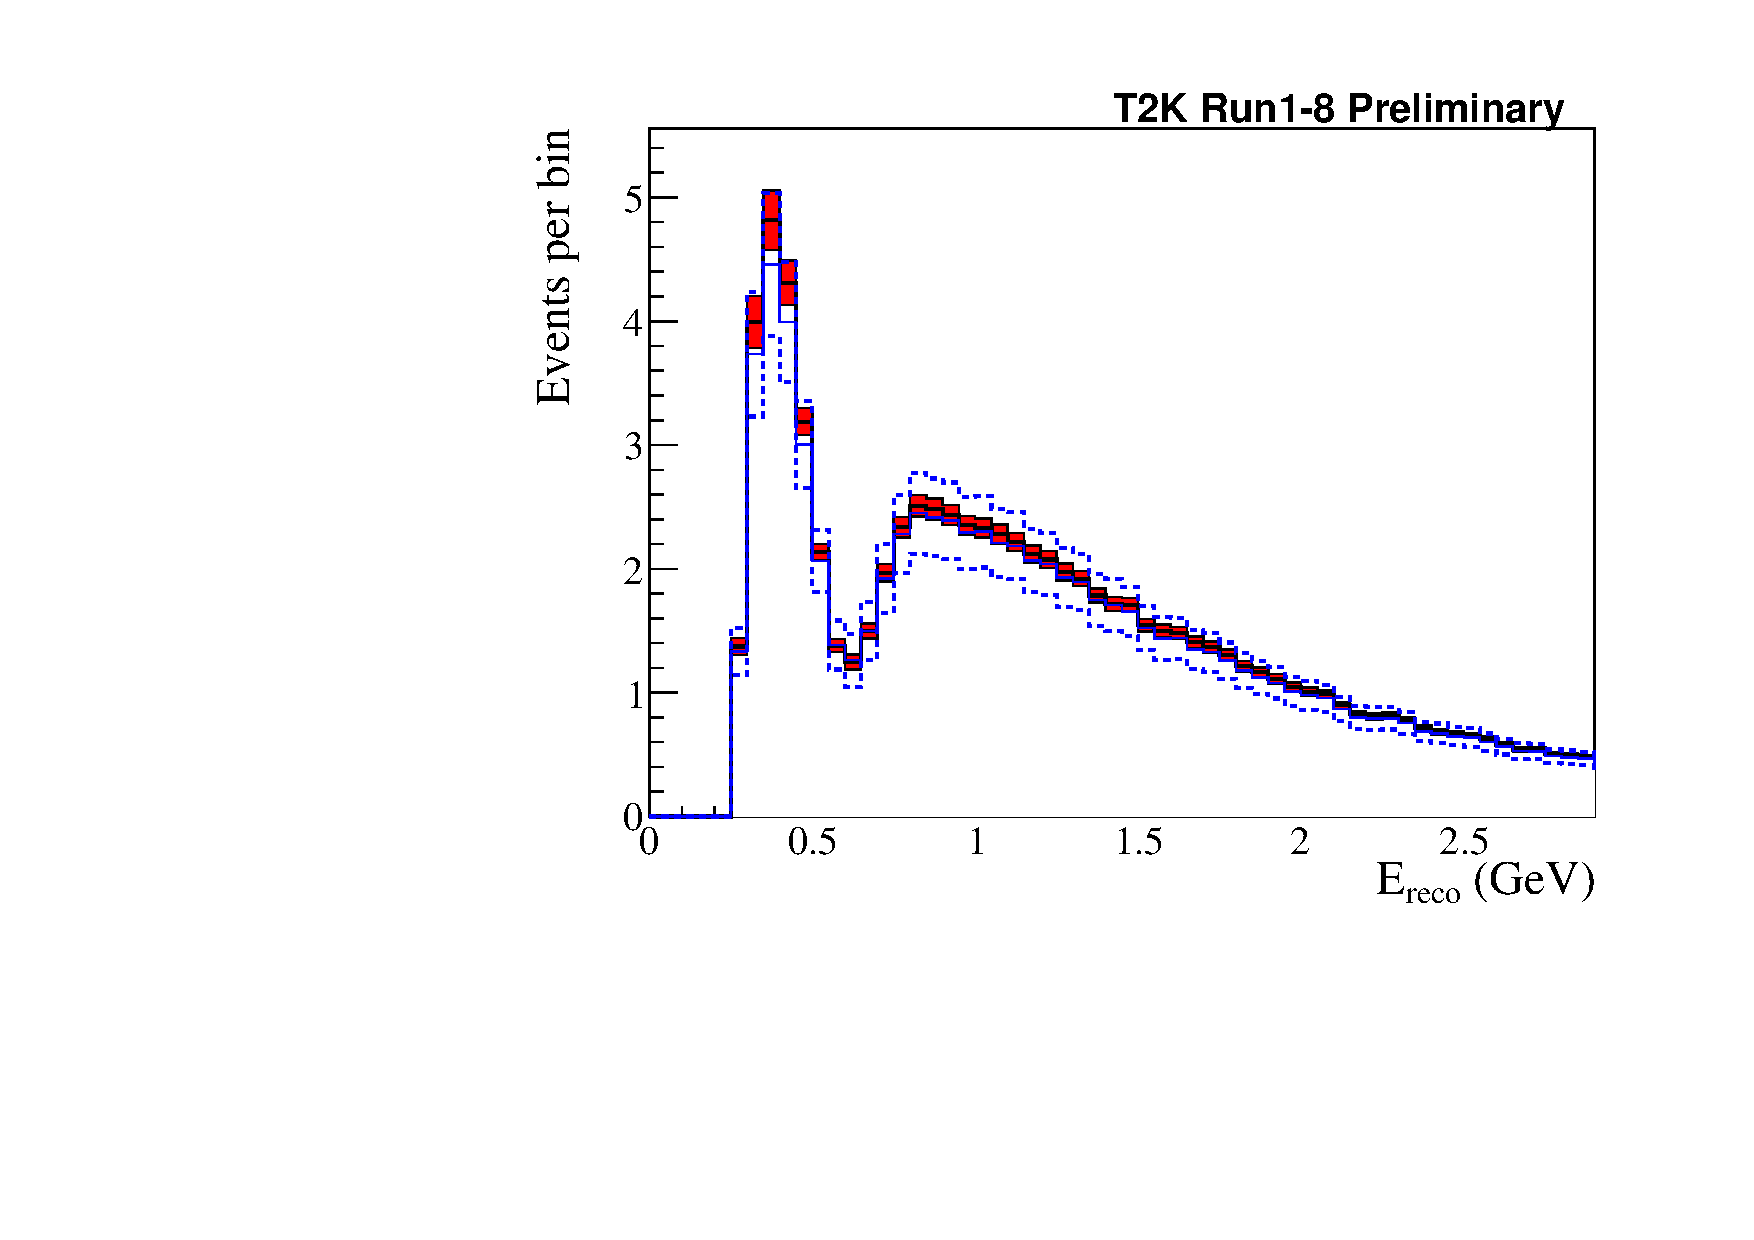
\includegraphics[width=0.9\textwidth]{images/systematics/envelopes/sk_error_table_RHC1Rmu_banff_constrained_envelope}
		\caption{Muon-like, antineutrino mode}
	\end{subfigure}
	\begin{subfigure}[b]{0.49\textwidth}
		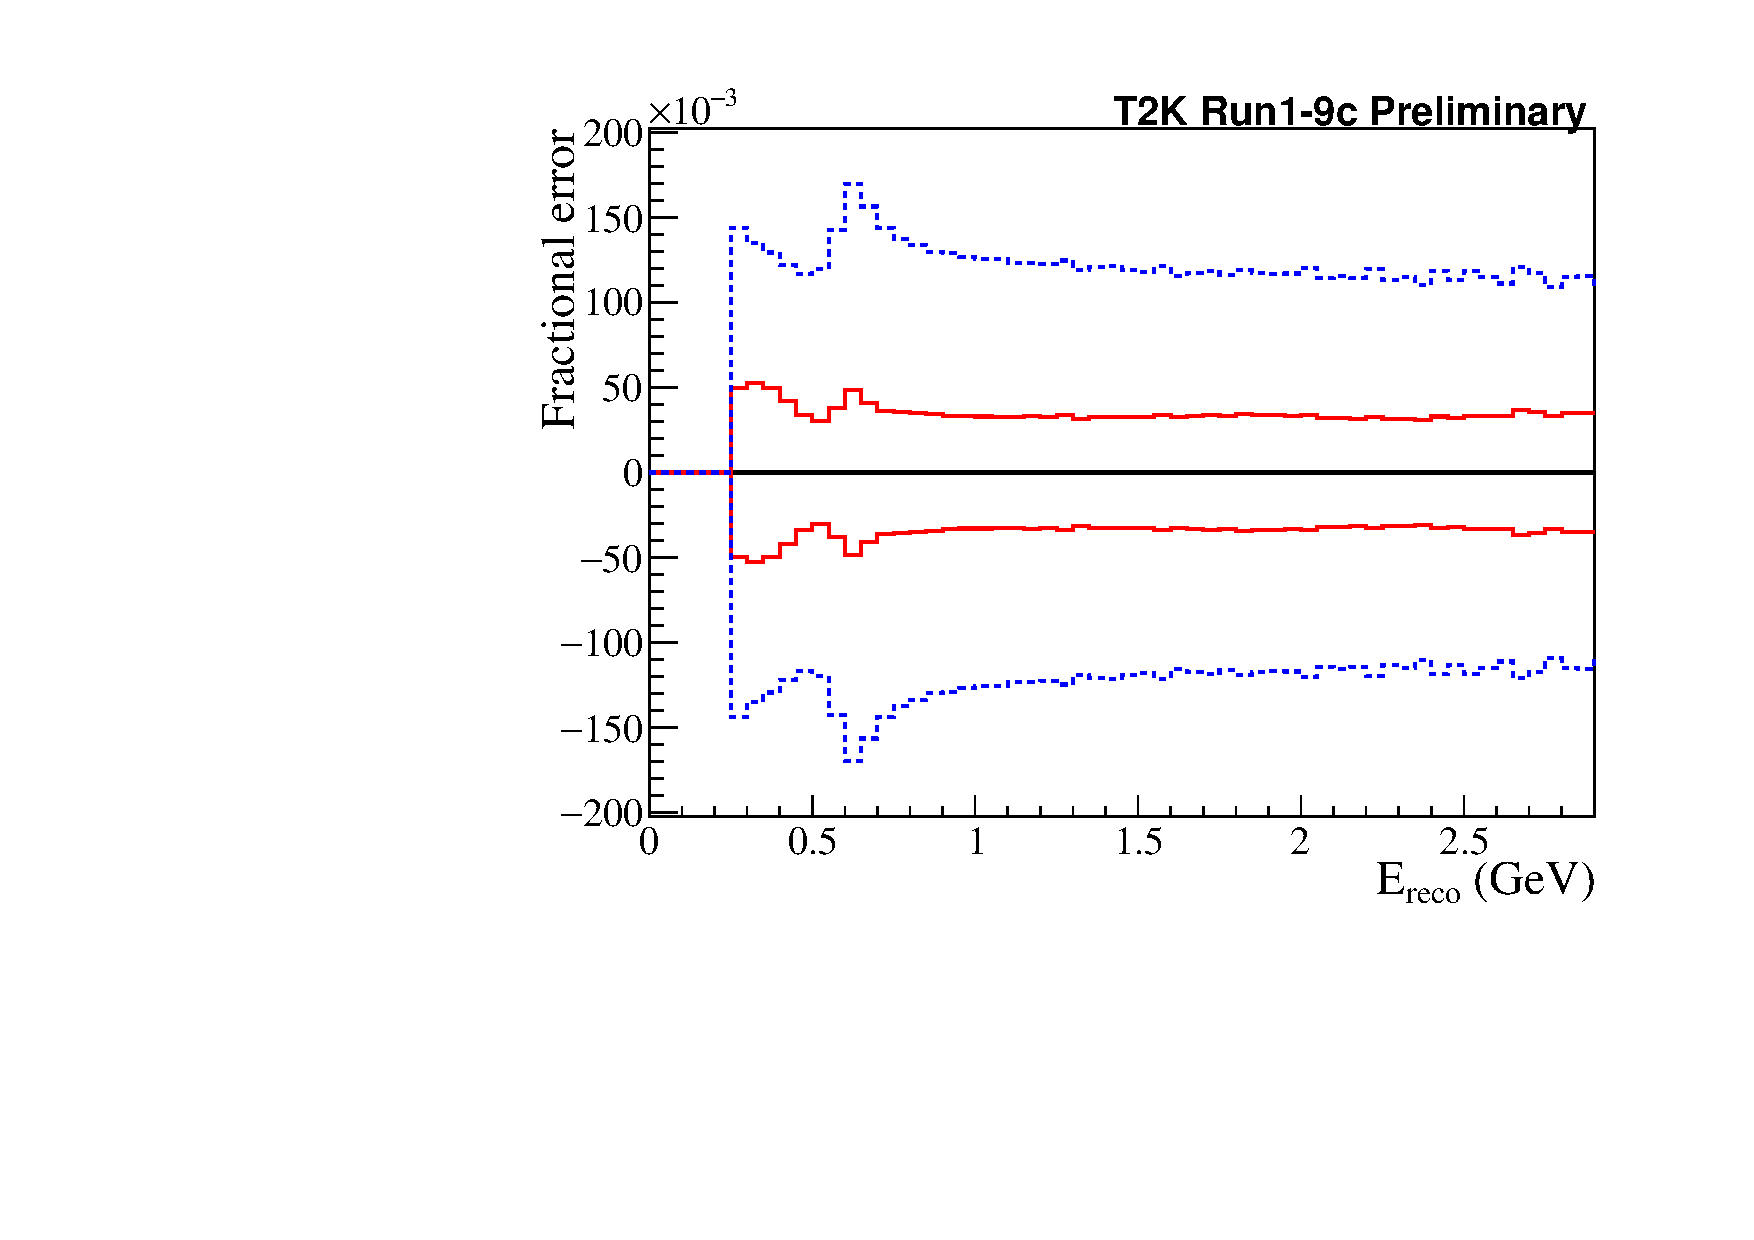
\includegraphics[width=0.9\textwidth]{images/systematics/envelopes/sk_error_table_RHC1Rmu_banff_constrained_envelope_fractional}
		\caption{Muon-like, antineutrino mode}
	\end{subfigure}
	\begin{subfigure}[b]{0.49\textwidth}
		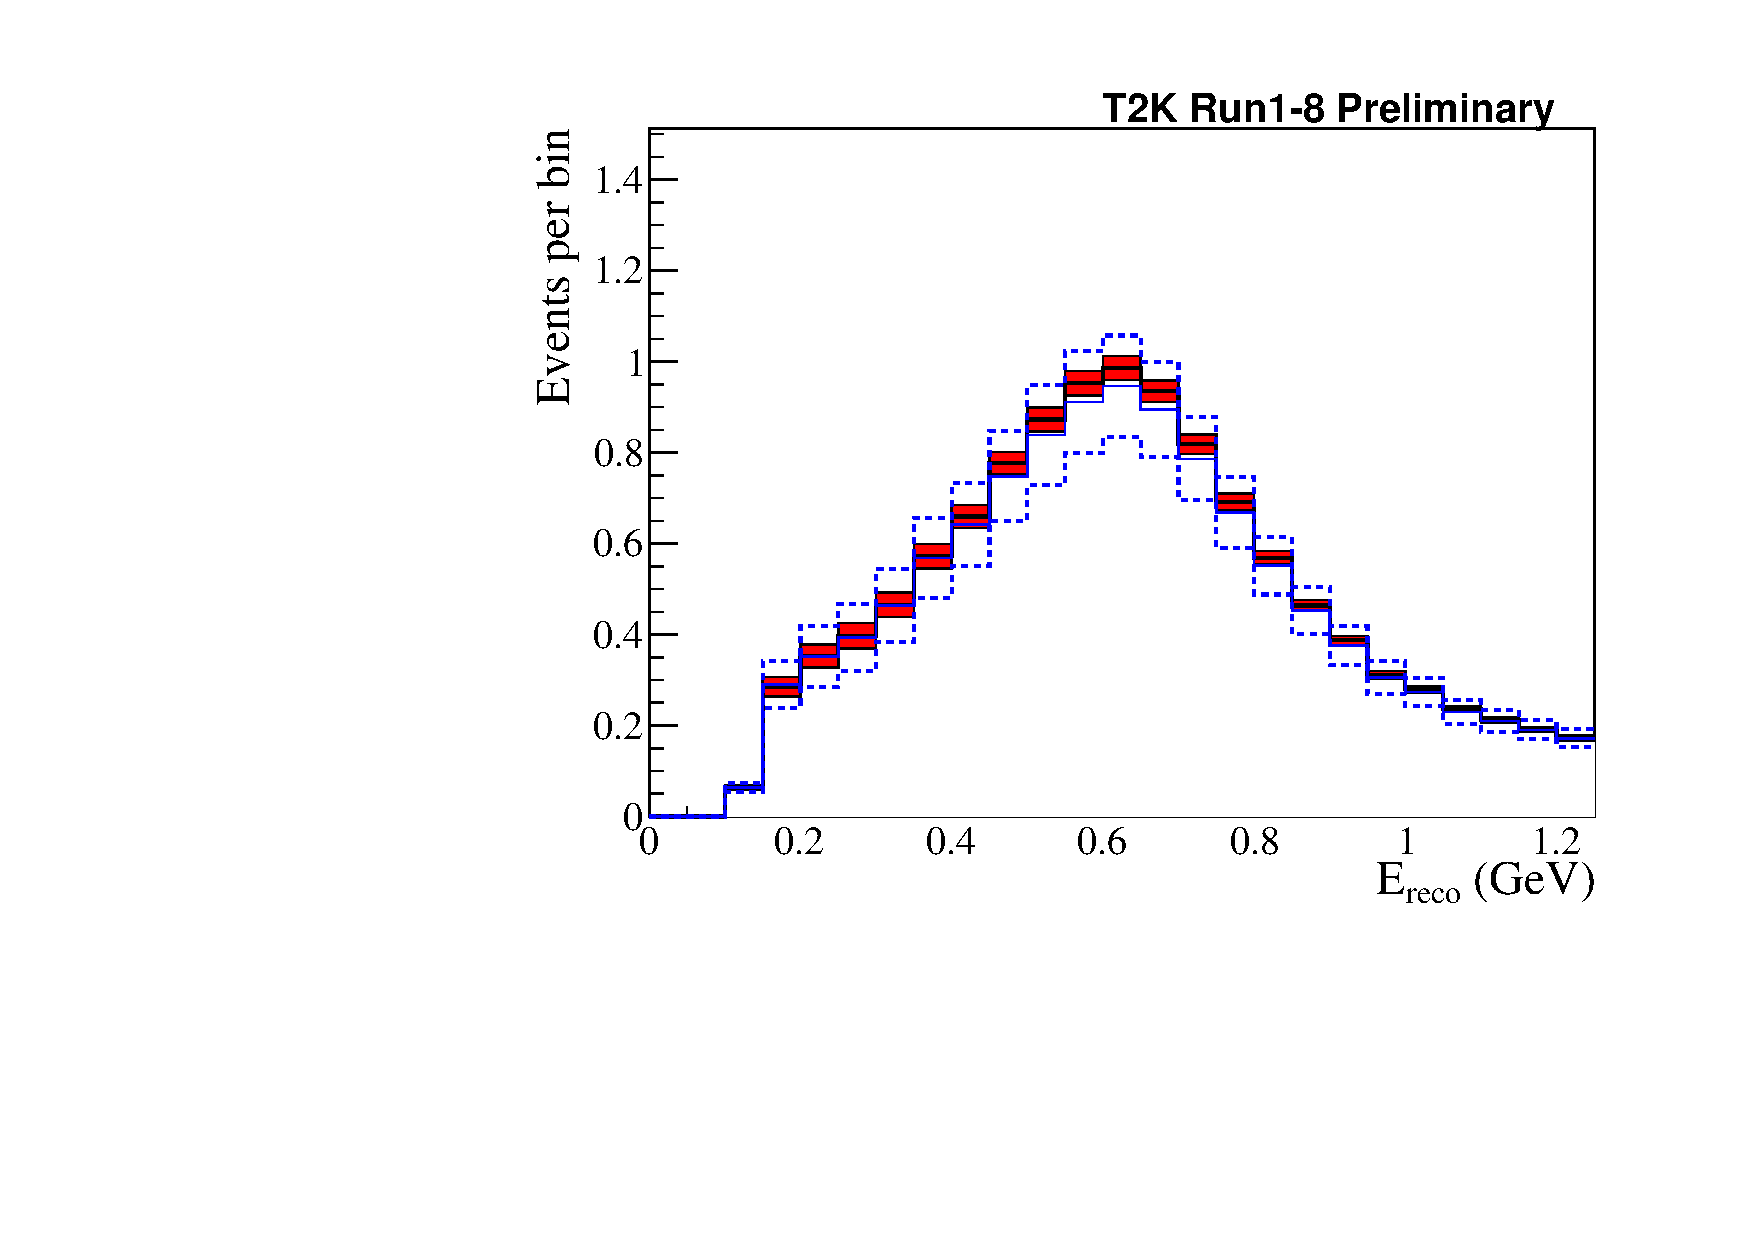
\includegraphics[width=0.9\textwidth]{images/systematics/envelopes/sk_error_table_RHC1Re_banff_constrained_envelope}
		\caption{Electron-like antineutrino mode}
	\end{subfigure}
	\begin{subfigure}[b]{0.49\textwidth}
		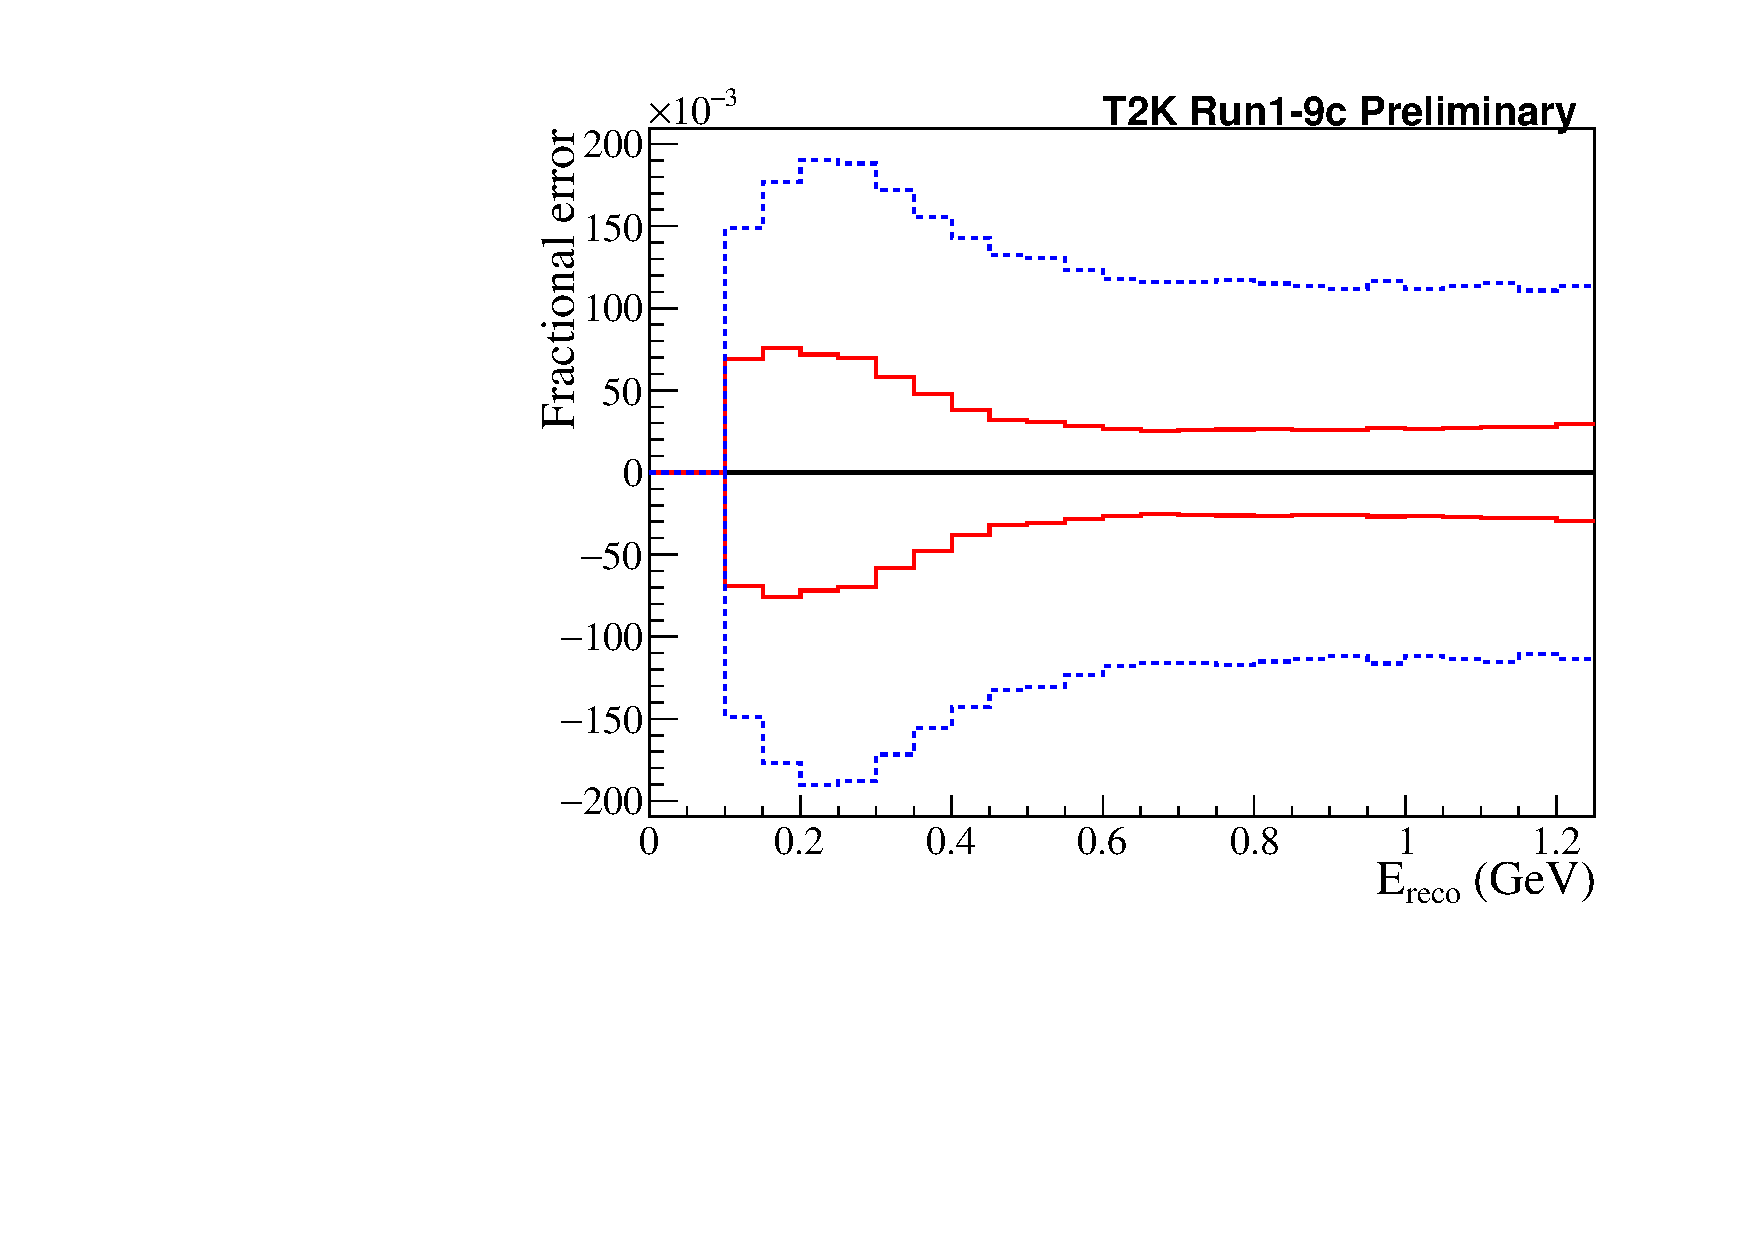
\includegraphics[width=0.9\textwidth]{images/systematics/envelopes/sk_error_table_RHC1Re_banff_constrained_envelope_fractional}
		\caption{Electron-like antineutrino mode}
	\end{subfigure}
	\caption {
		Error envelopes (left) and fractional error (right) for the reconstructed neutrino energy spectrum for the flux and constrained cross-section systematic parameters for pre-BANFF (blue) and post-BANFF (red) errors. \NumToysSmall toys are generated for the Asimov data set A with randomized systematic parameters with correlations taken into account.
	}
	\label{fig:sk_envelopes_banff_b}
\end{figure*}
\clearpage
\begin{figure*}
	\center
	\begin{subfigure}[b]{0.49\textwidth}
		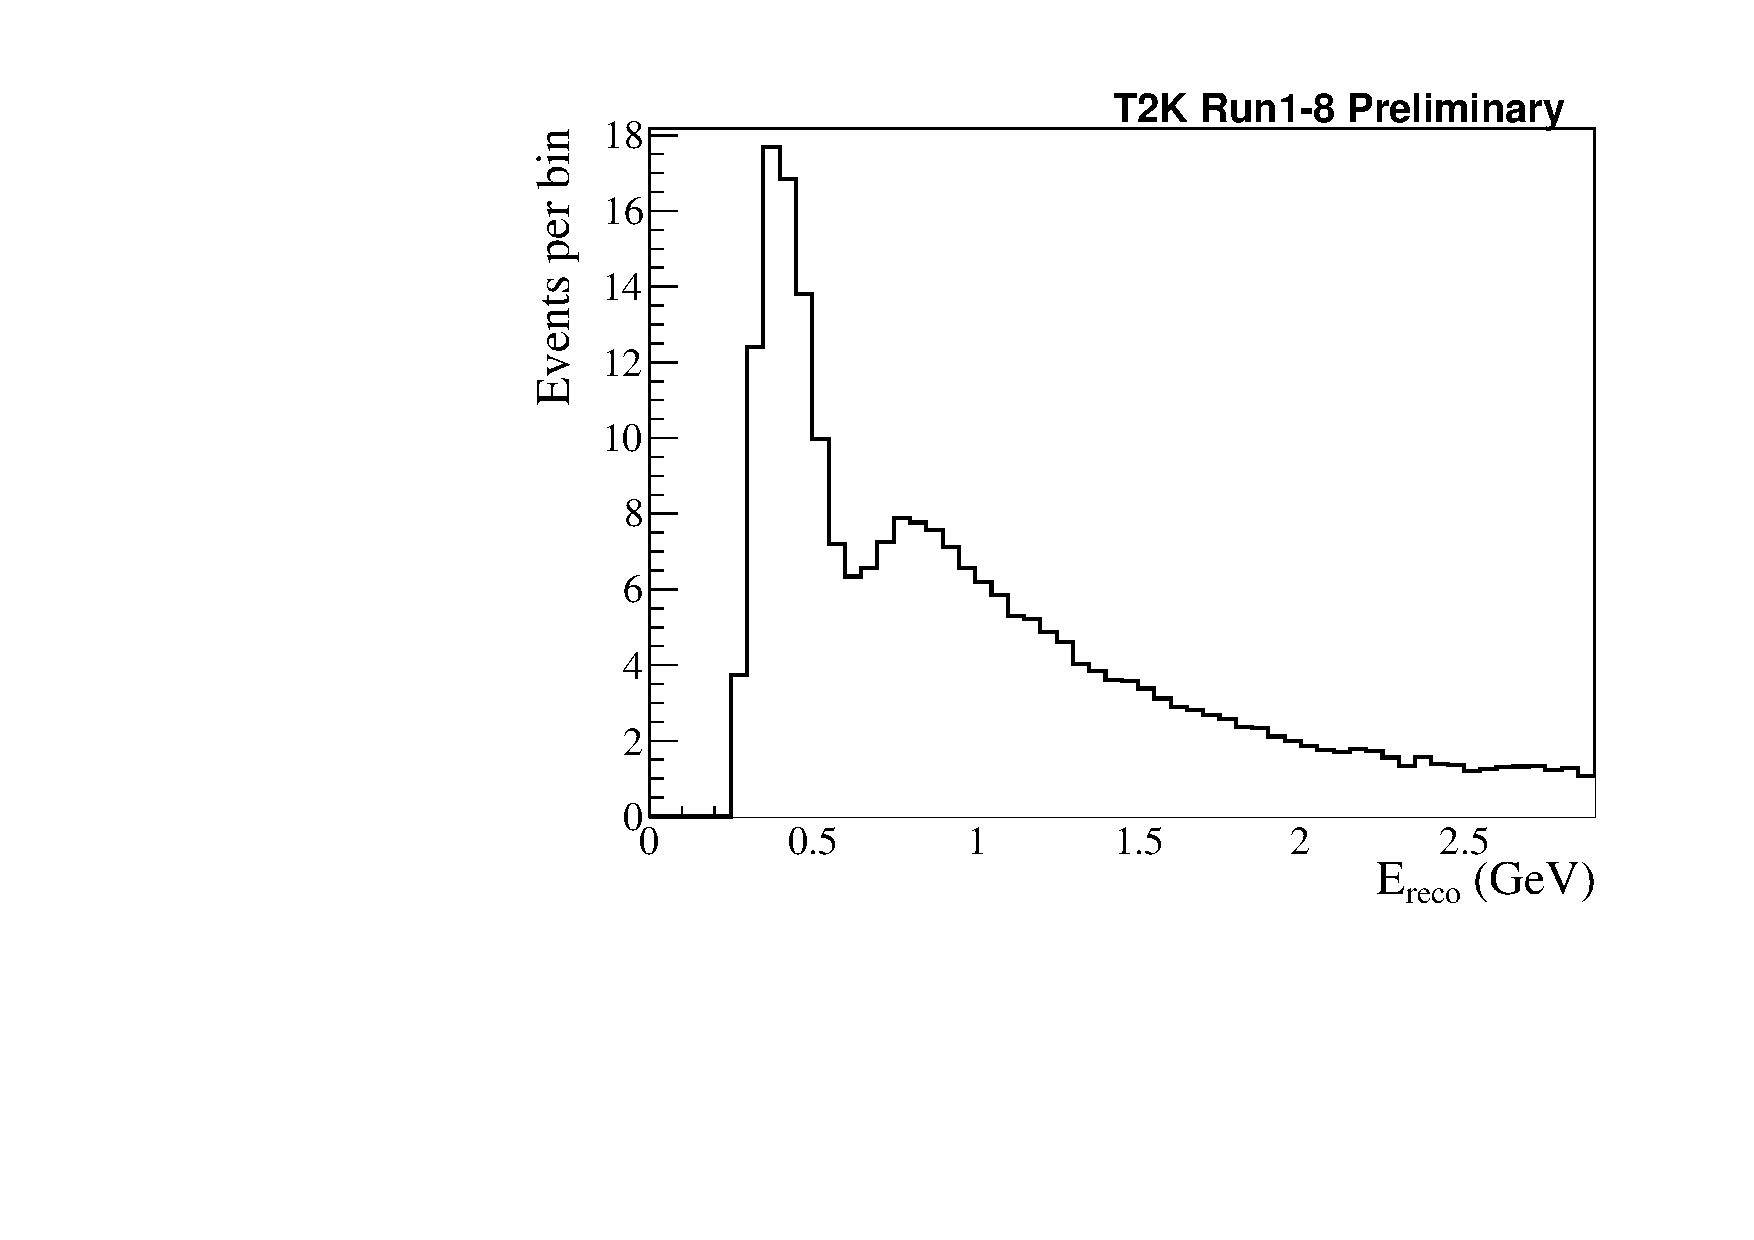
\includegraphics[width=0.9\textwidth]{images/systematics/envelopes/sk_error_table_1Rmu_xsec_nue_envelope}
		\caption{Muon-like, neutrino mode}
	\end{subfigure}
	\begin{subfigure}[b]{0.49\textwidth}
		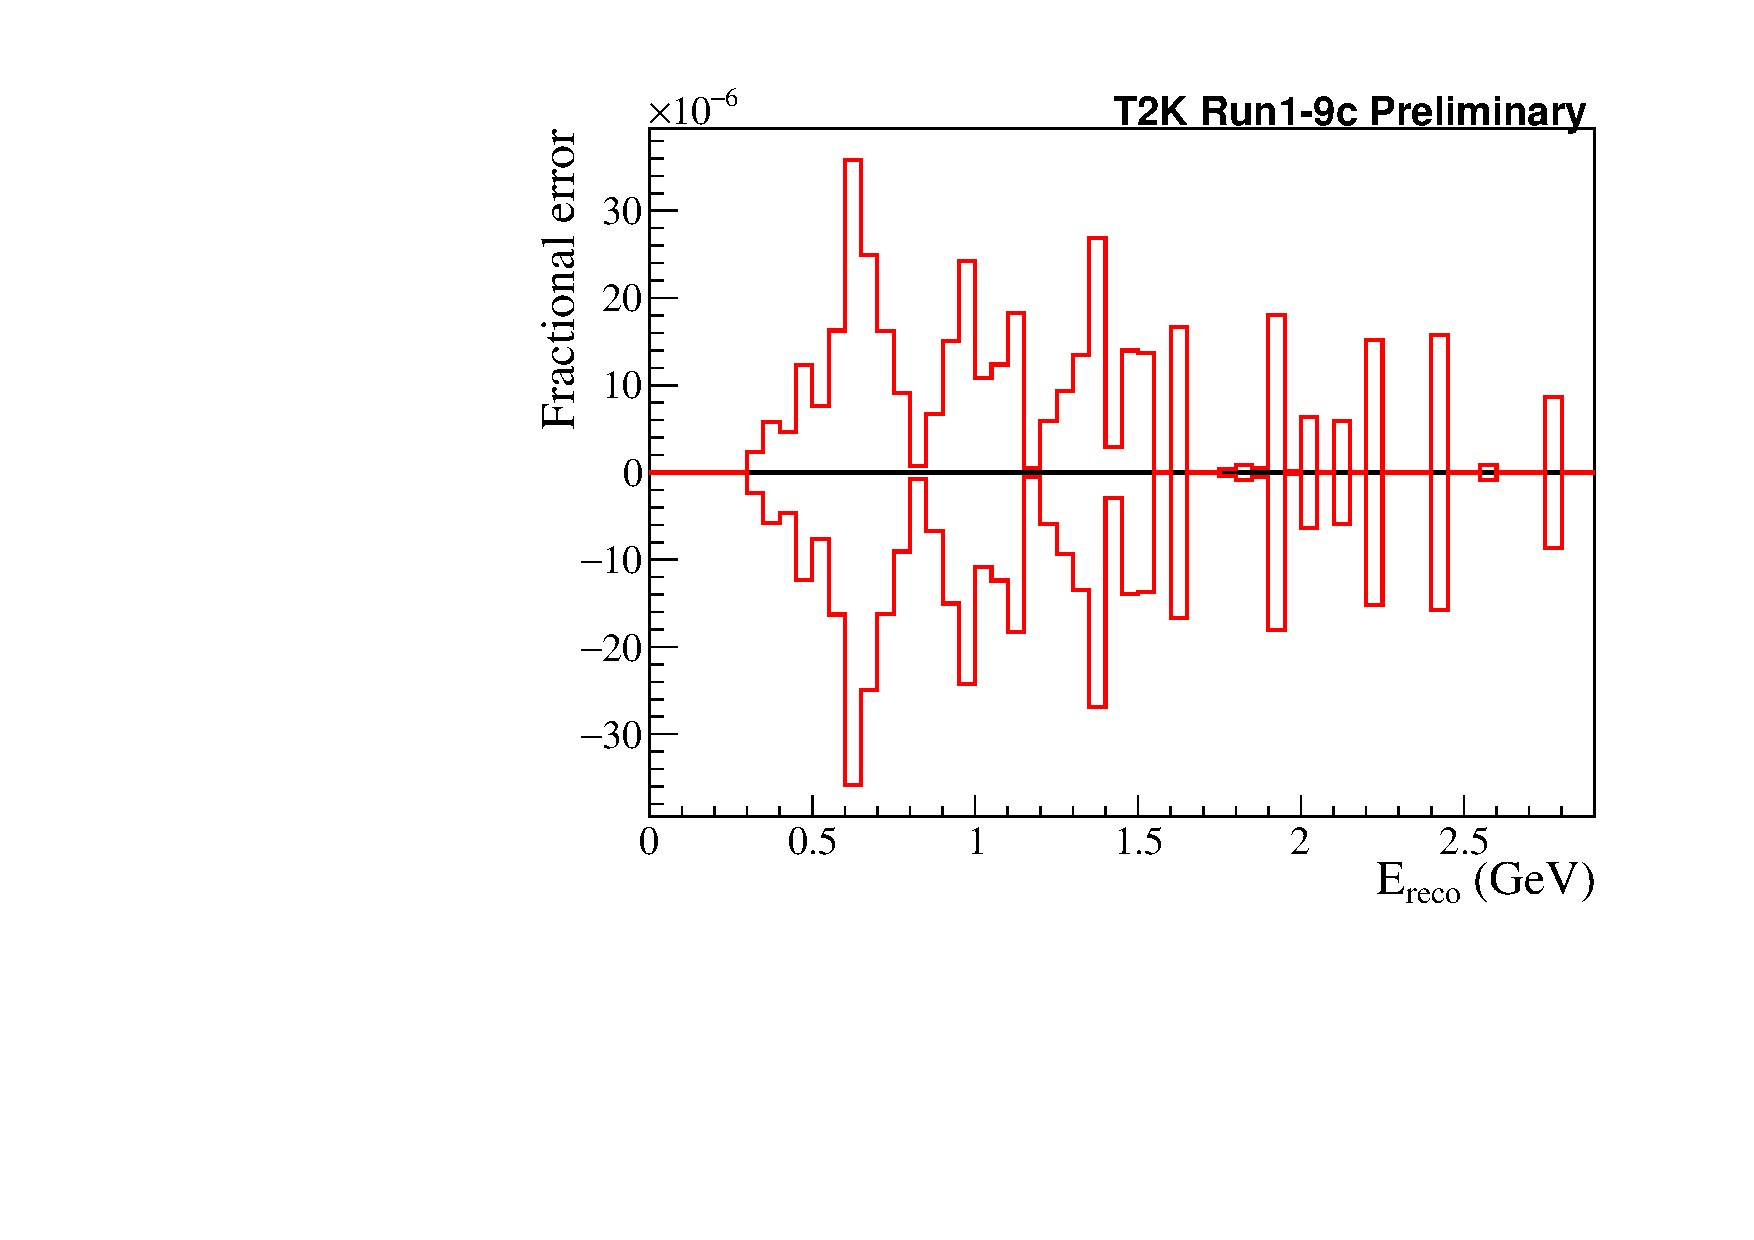
\includegraphics[width=0.9\textwidth]{images/systematics/envelopes/sk_error_table_1Rmu_xsec_nue_envelope_fractional}
		\caption{Muon-like, neutrino mode}
	\end{subfigure}
	\begin{subfigure}[b]{0.49\textwidth}
		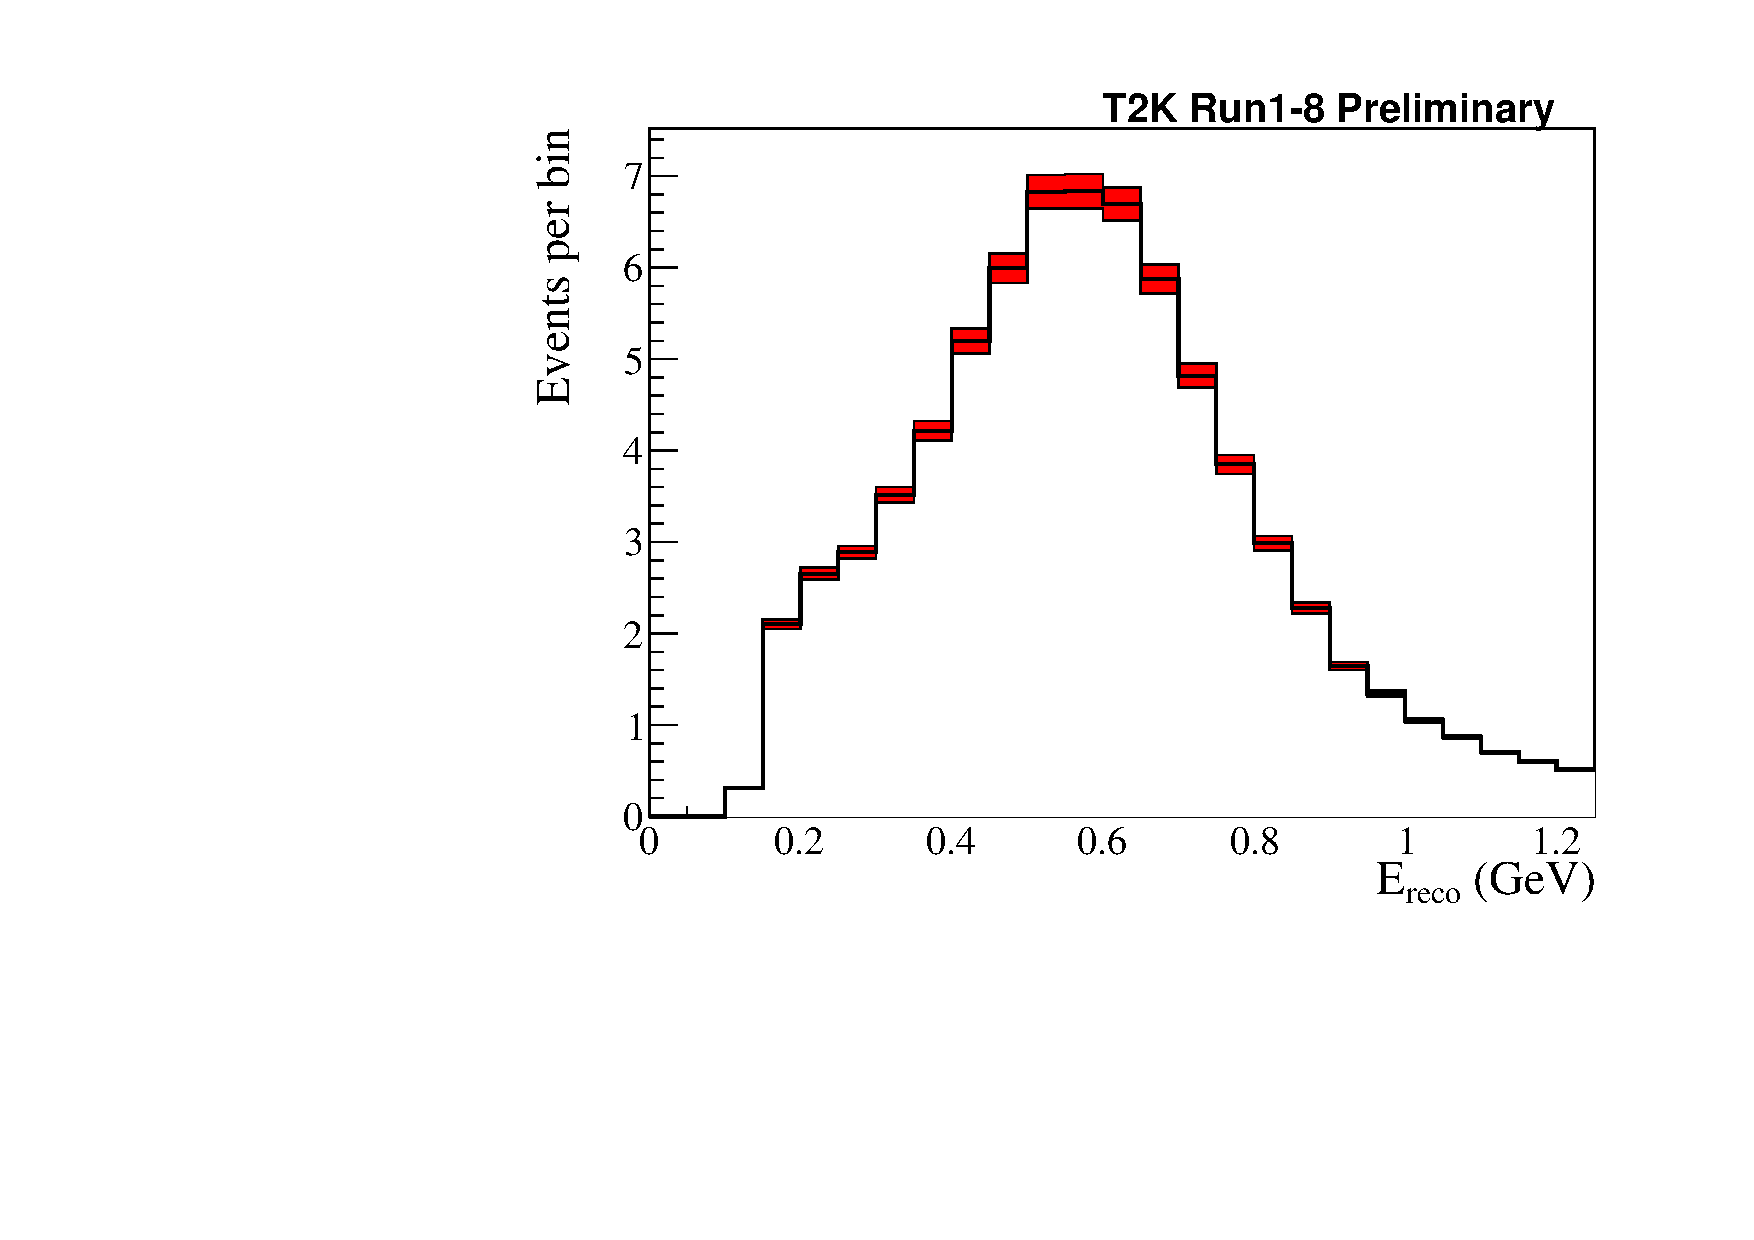
\includegraphics[width=0.9\textwidth]{images/systematics/envelopes/sk_error_table_1Re_xsec_nue_envelope}
		\caption{Electron-like, neutrino mode}
	\end{subfigure}
	\begin{subfigure}[b]{0.49\textwidth}
		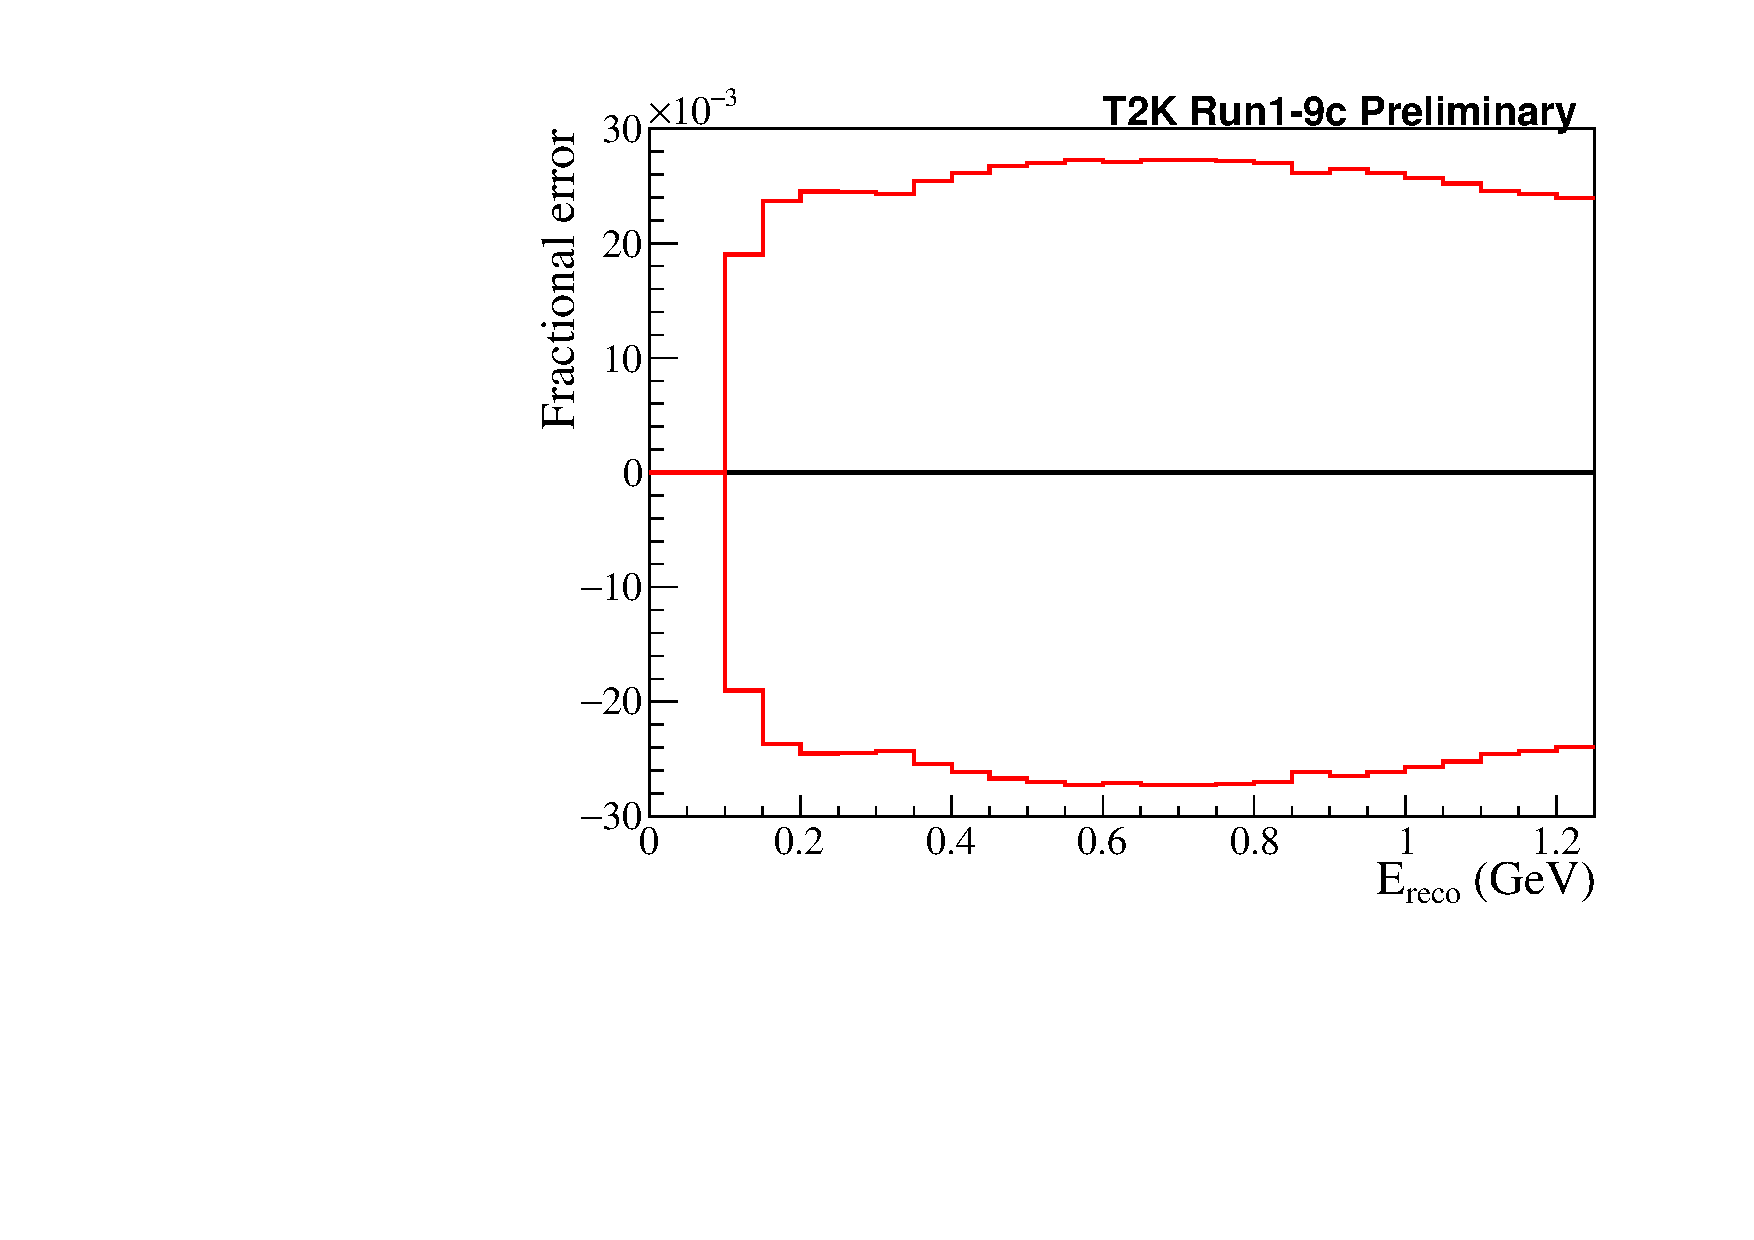
\includegraphics[width=0.9\textwidth]{images/systematics/envelopes/sk_error_table_1Re_xsec_nue_envelope_fractional}
		\caption{Electron-like, neutrino mode}
	\end{subfigure}
	\begin{subfigure}[b]{0.49\textwidth}
		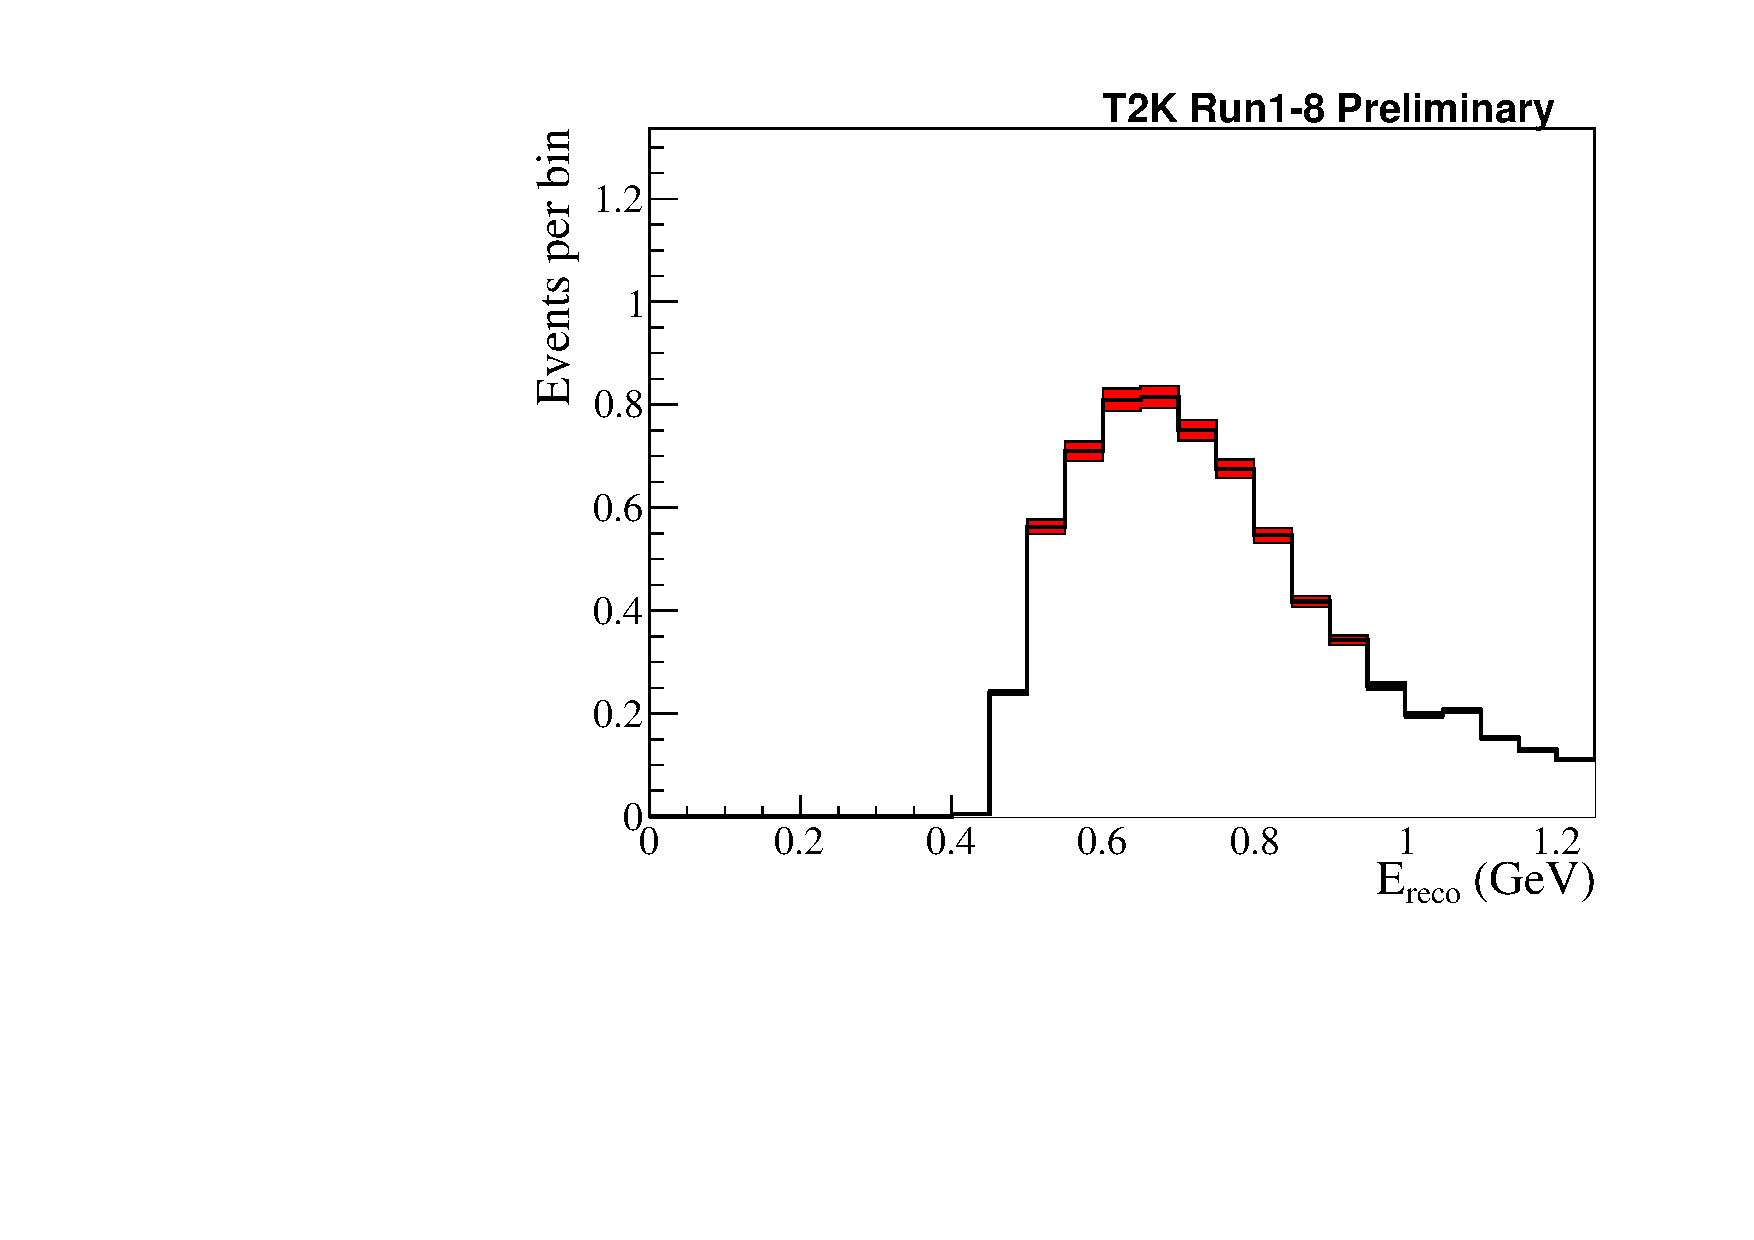
\includegraphics[width=0.9\textwidth]{images/systematics/envelopes/sk_error_table_MultiRe_xsec_nue_envelope}
		\caption{\nueCConepi-like, neutrino mode}
	\end{subfigure}
	\begin{subfigure}[b]{0.49\textwidth}
		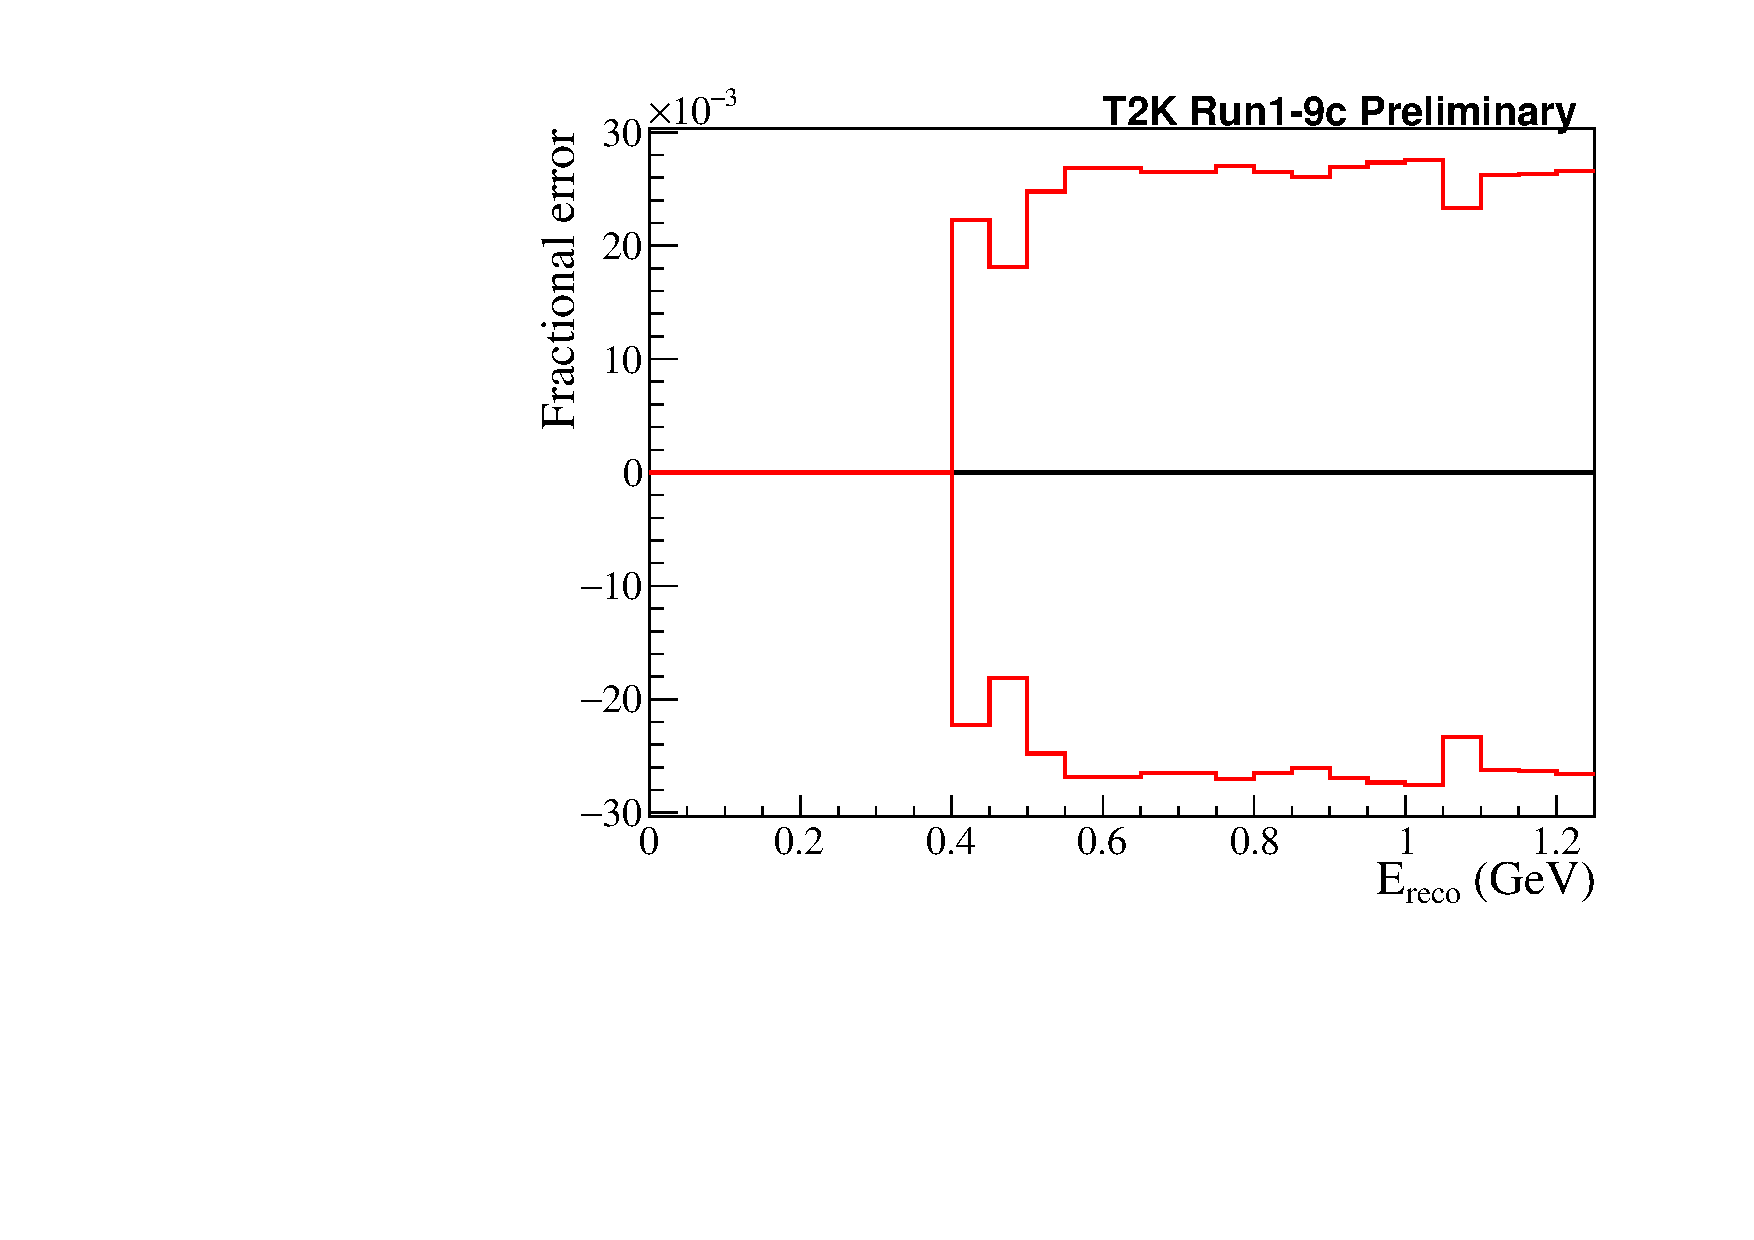
\includegraphics[width=0.9\textwidth]{images/systematics/envelopes/sk_error_table_MultiRe_xsec_nue_envelope_fractional}
		\caption{\nueCConepi-like, neutrino mode}
	\end{subfigure}
	\caption {
		Error envelopes (left) and fractional errors (right) for the reconstructed neutrino energy spectrum for the unconstrained electron neutrino cross-section systematic parameters. \NumToysSmall toys are generated for the Asimov data set A with randomized systematic parameters with correlations taken into account.
	}
	\label{fig:sk_envelopes_xsec_nue}
\end{figure*}
\clearpage

\begin{figure*}
	\center
	\begin{subfigure}[b]{0.49\textwidth}
		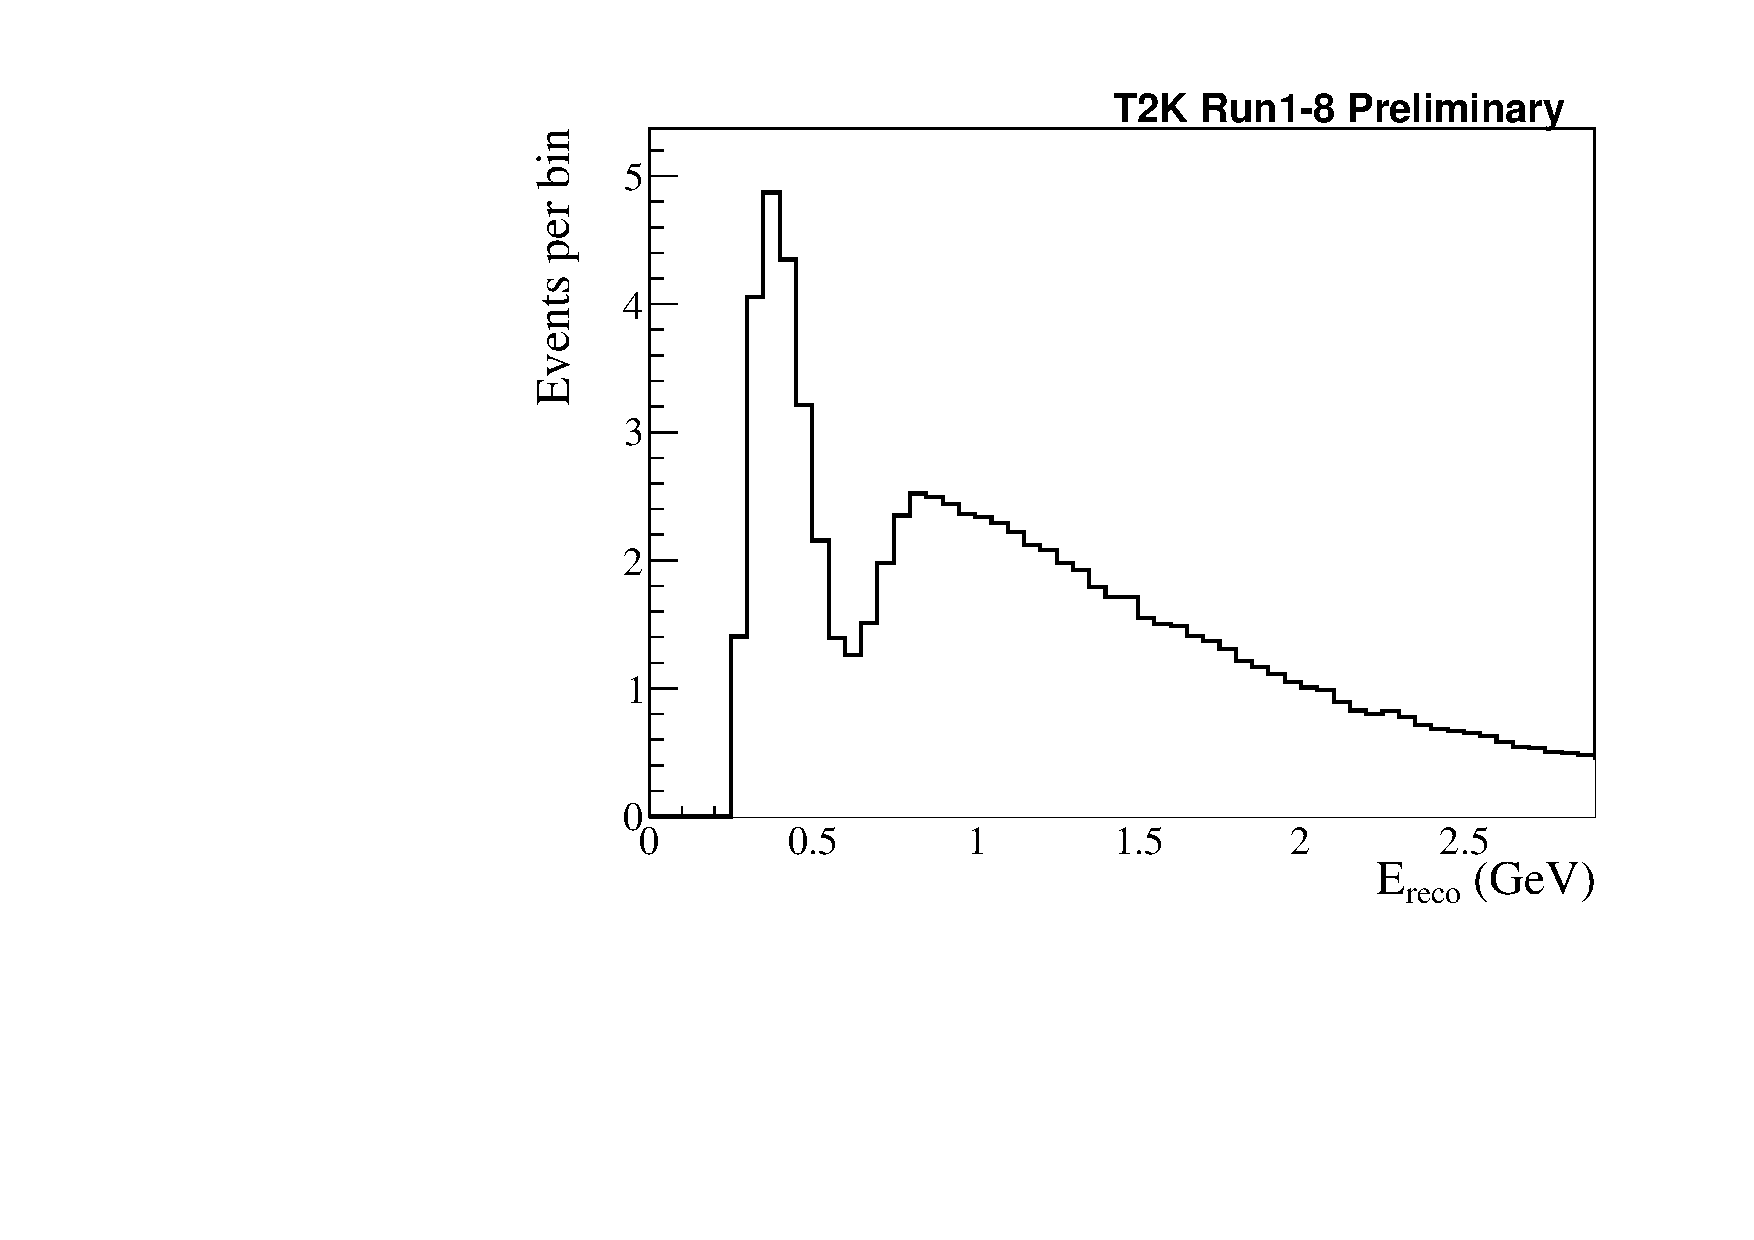
\includegraphics[width=0.9\textwidth]{images/systematics/envelopes/sk_error_table_RHC1Rmu_xsec_nue_envelope}
		\caption{Muon-like, antineutrino mode}
	\end{subfigure}
	\begin{subfigure}[b]{0.49\textwidth}
		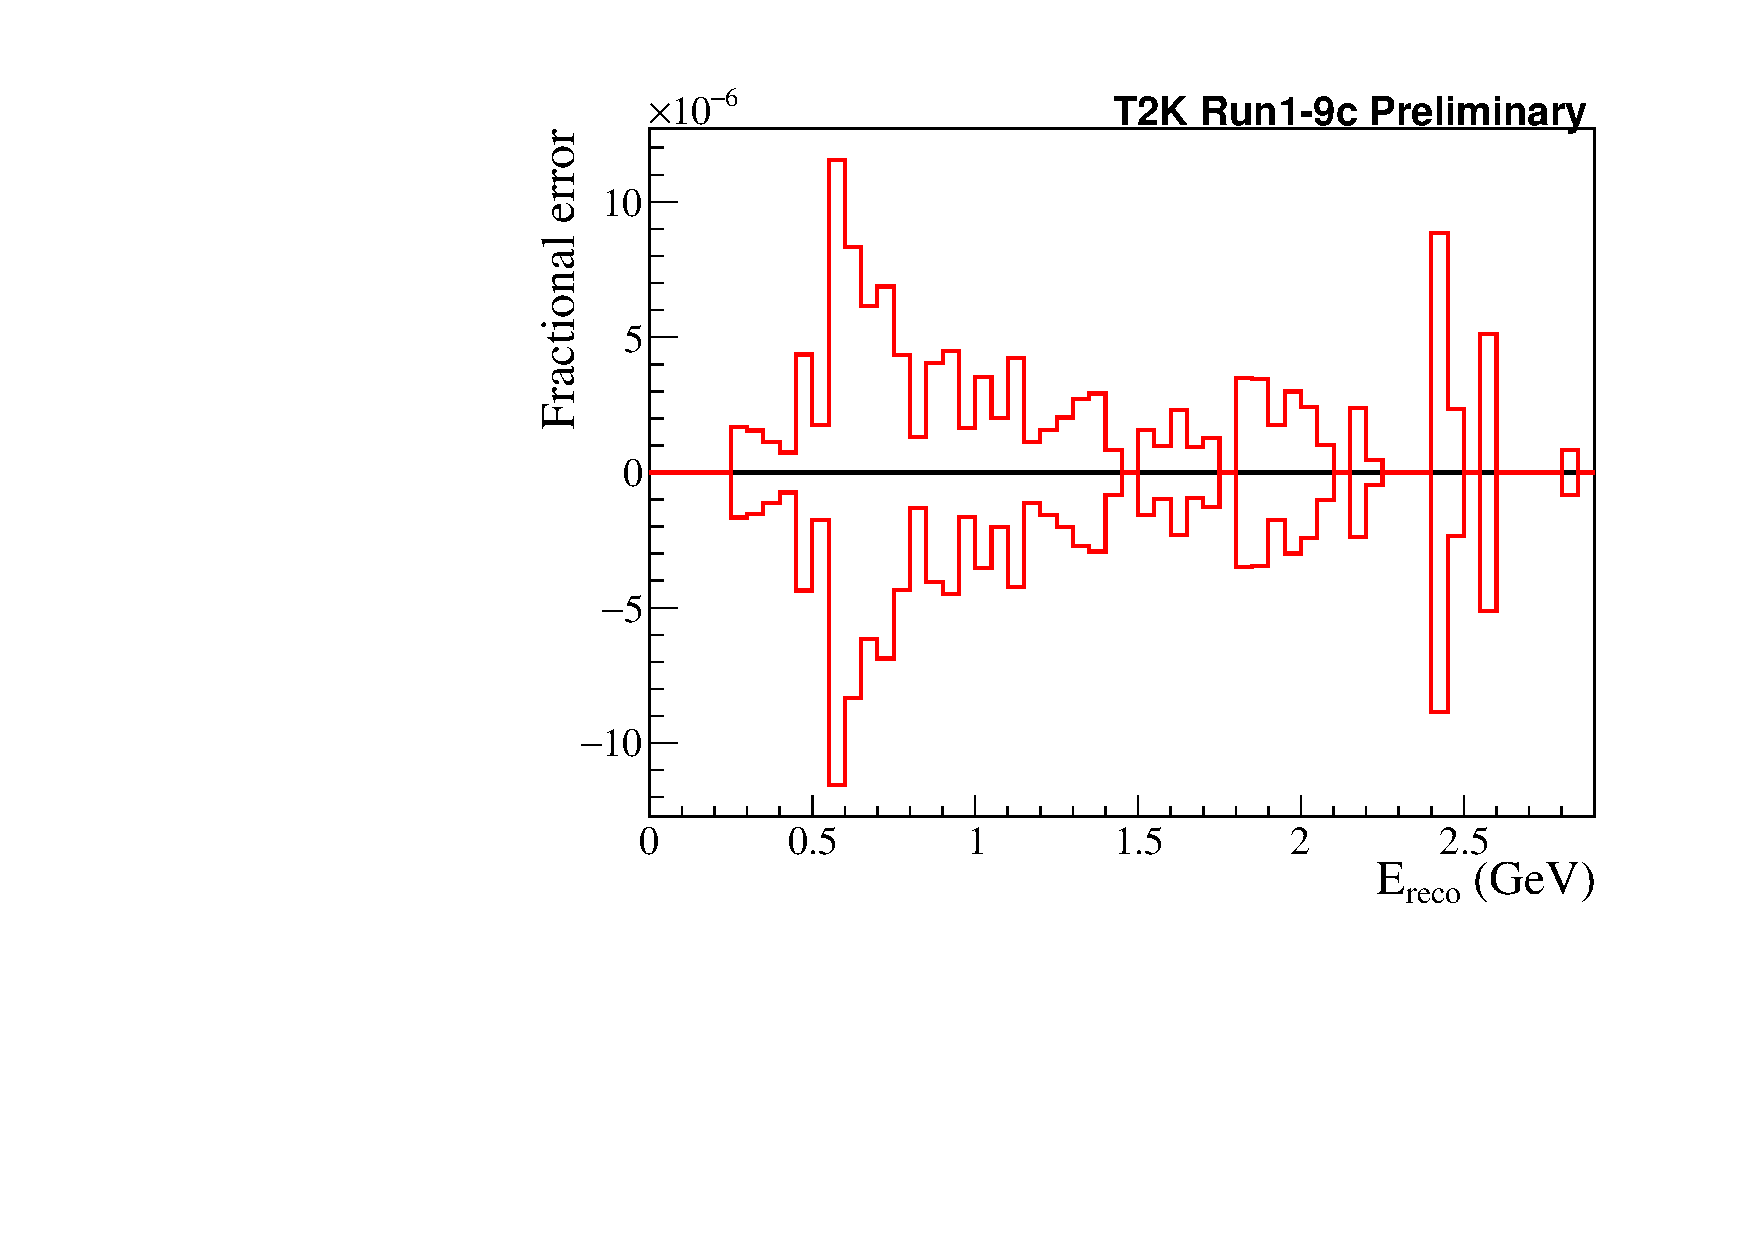
\includegraphics[width=0.9\textwidth]{images/systematics/envelopes/sk_error_table_RHC1Rmu_xsec_nue_envelope_fractional}
		\caption{Muon-like, antineutrino mode}
	\end{subfigure}
	\begin{subfigure}[b]{0.49\textwidth}
		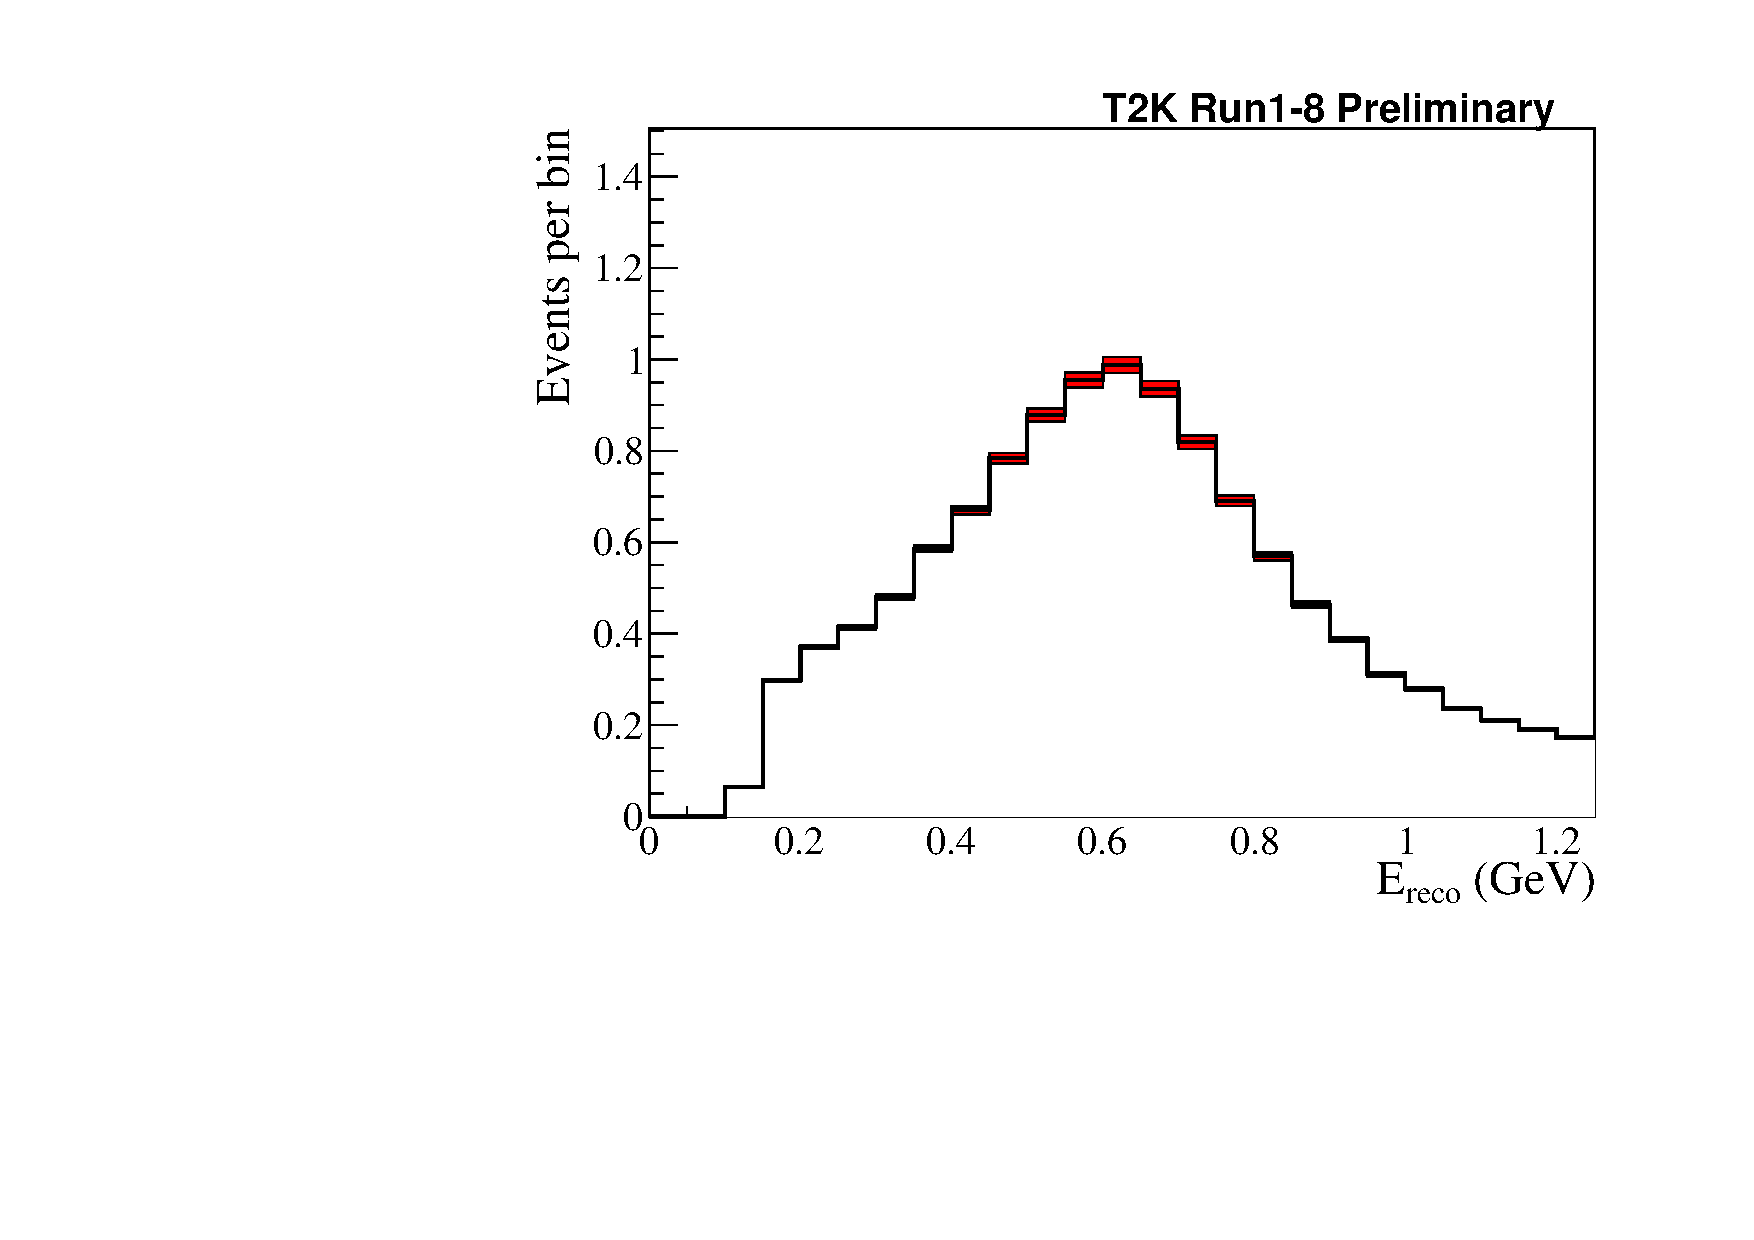
\includegraphics[width=0.9\textwidth]{images/systematics/envelopes/sk_error_table_RHC1Re_xsec_nue_envelope}
		\caption{Electron-like antineutrino mode}
	\end{subfigure}
	\begin{subfigure}[b]{0.49\textwidth}
		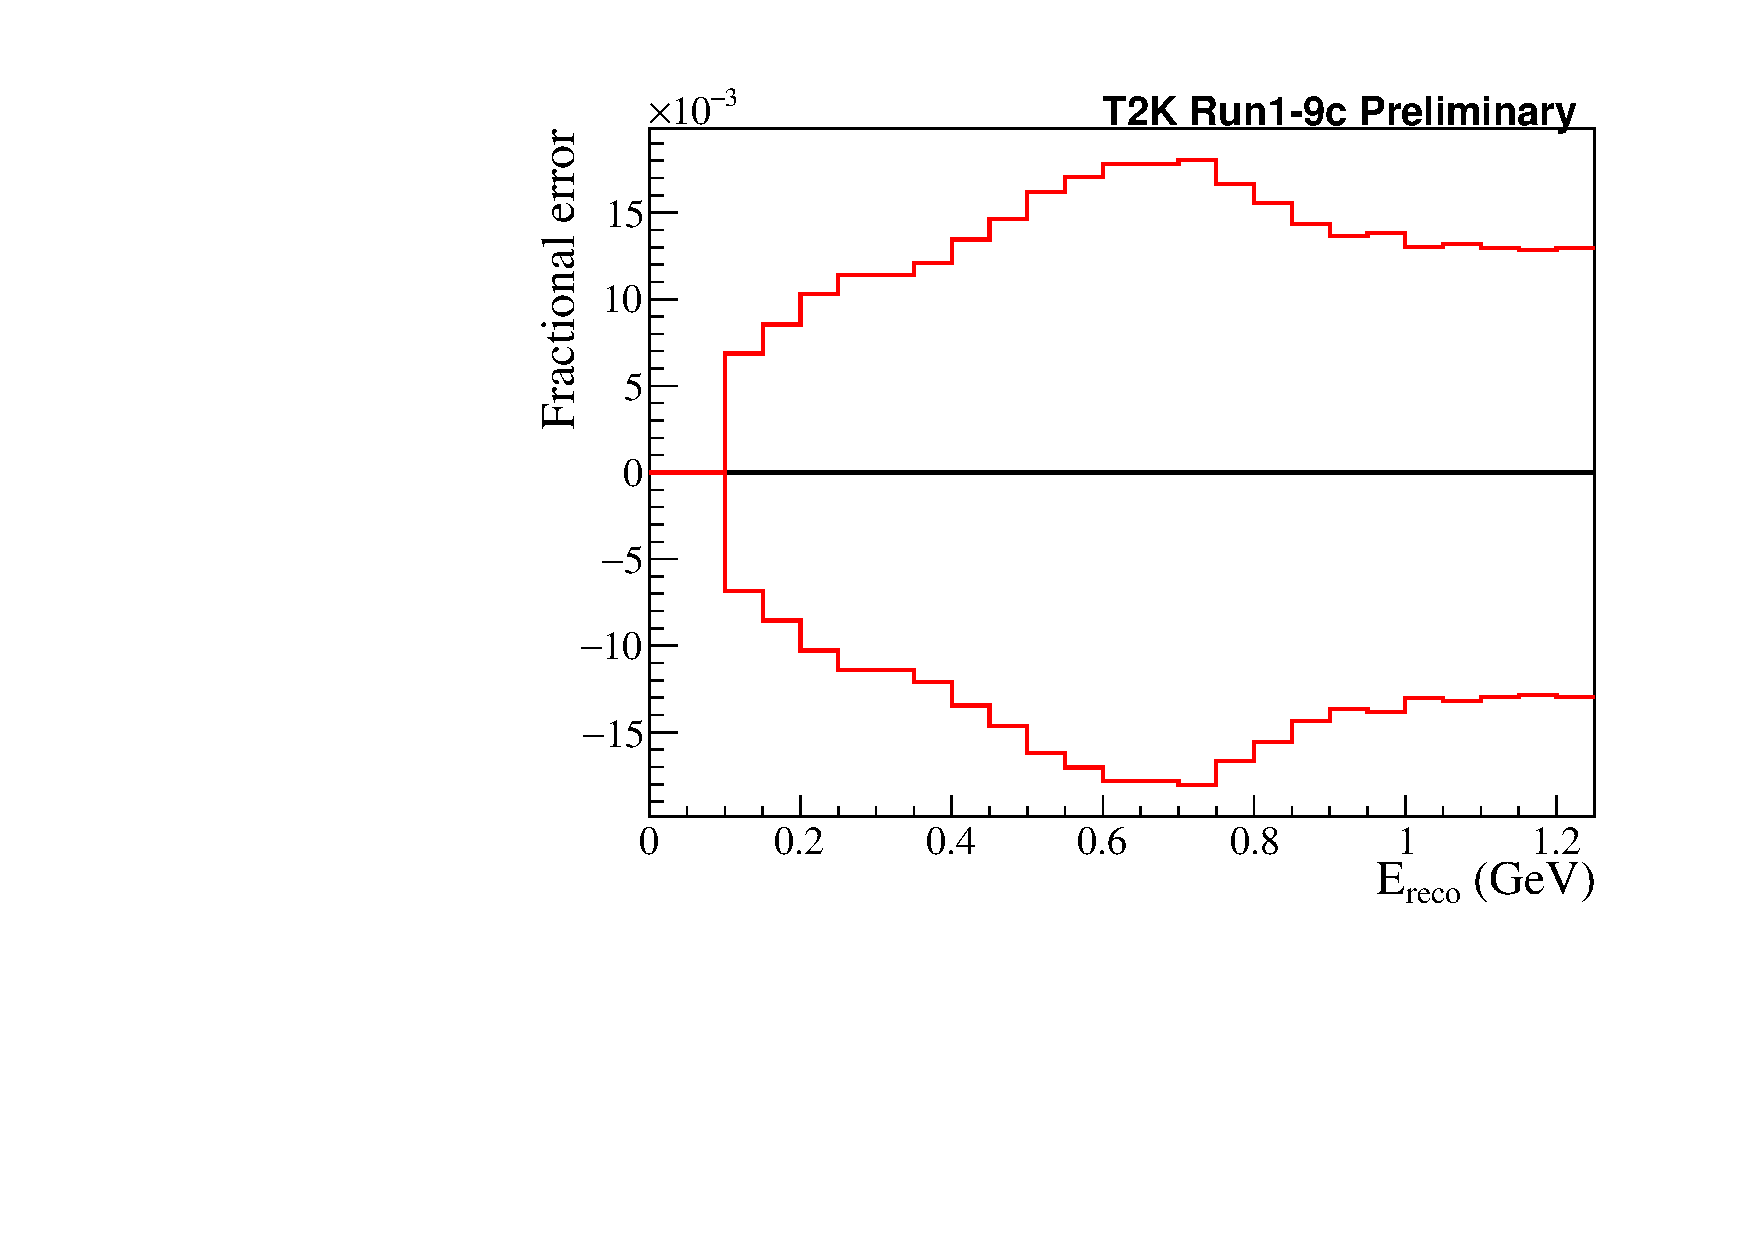
\includegraphics[width=0.9\textwidth]{images/systematics/envelopes/sk_error_table_RHC1Re_xsec_nue_envelope_fractional}
		\caption{Electron-like antineutrino mode}
	\end{subfigure}
	\caption {
		Error envelopes (left) and fractional errors (right) for the reconstructed neutrino energy spectrum for the unconstrained electron neutrino cross-section systematic parameters. \NumToysSmall toys are generated for the Asimov data set A with randomized systematic parameters with correlations taken into account.
	}
	\label{fig:sk_envelopes_xsec_nue_b}
\end{figure*}
\clearpage
\begin{figure*}
	\center
	\begin{subfigure}[b]{0.49\textwidth}
		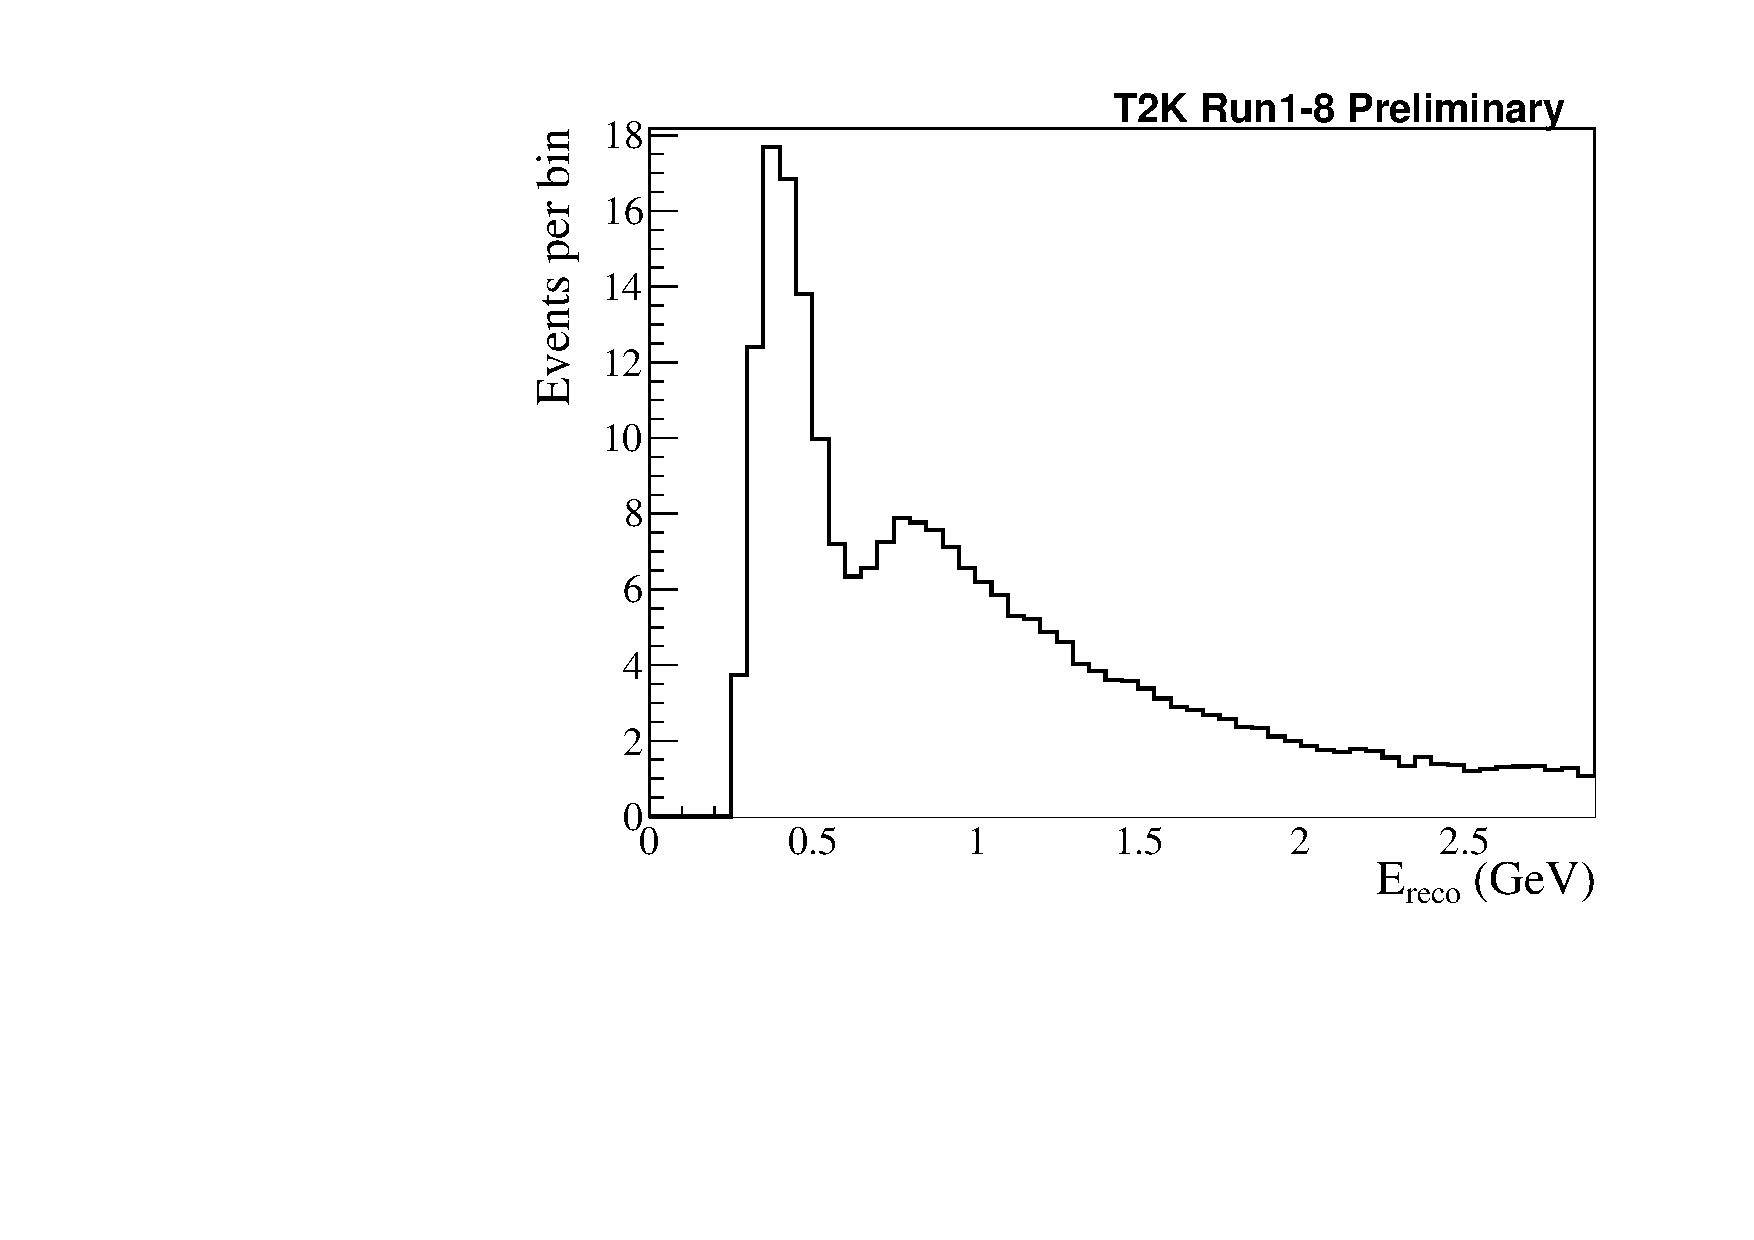
\includegraphics[width=0.9\textwidth]{images/systematics/envelopes/sk_error_table_1Rmu_xsec_ncgamma_envelope}
		\caption{Muon-like, neutrino mode}
	\end{subfigure}
	\begin{subfigure}[b]{0.49\textwidth}
		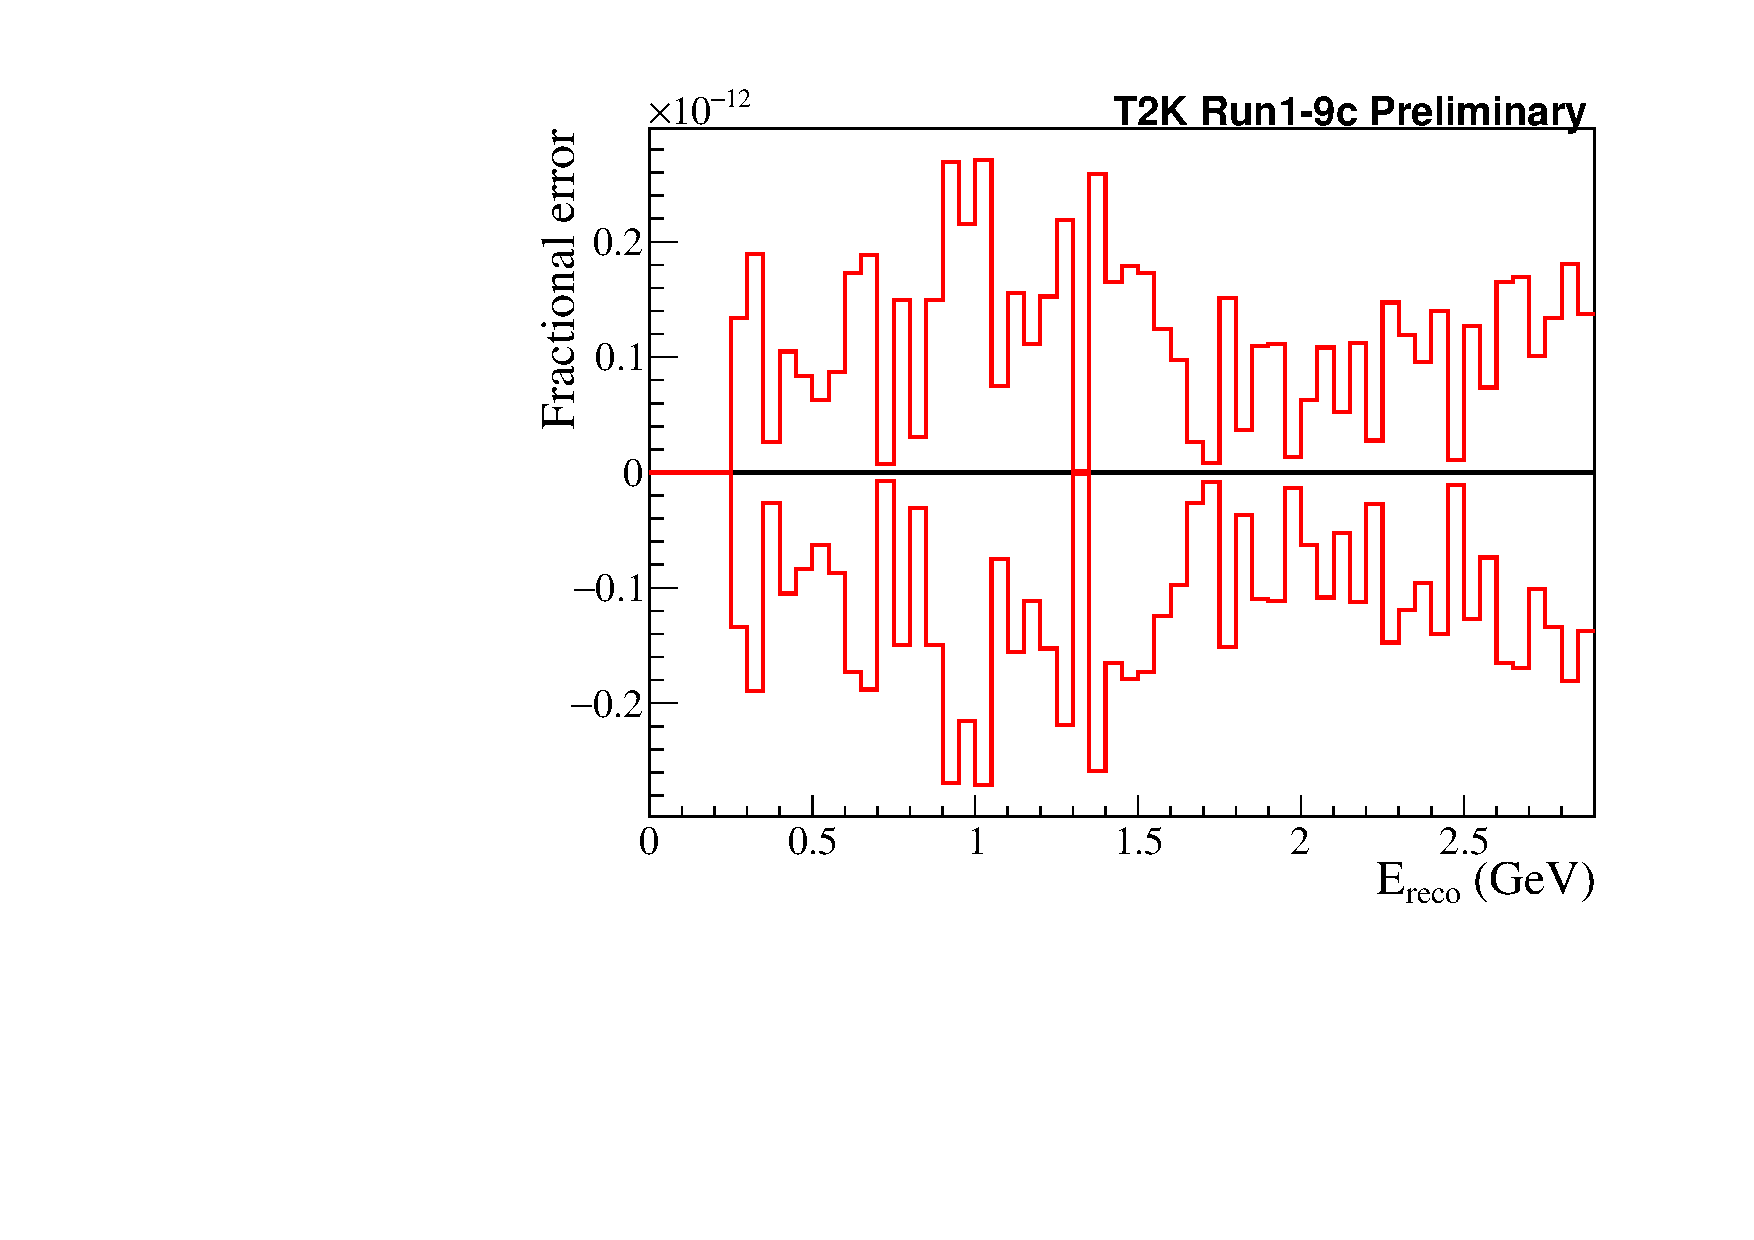
\includegraphics[width=0.9\textwidth]{images/systematics/envelopes/sk_error_table_1Rmu_xsec_ncgamma_envelope_fractional}
		\caption{Muon-like, neutrino mode}
	\end{subfigure}
	\begin{subfigure}[b]{0.49\textwidth}
		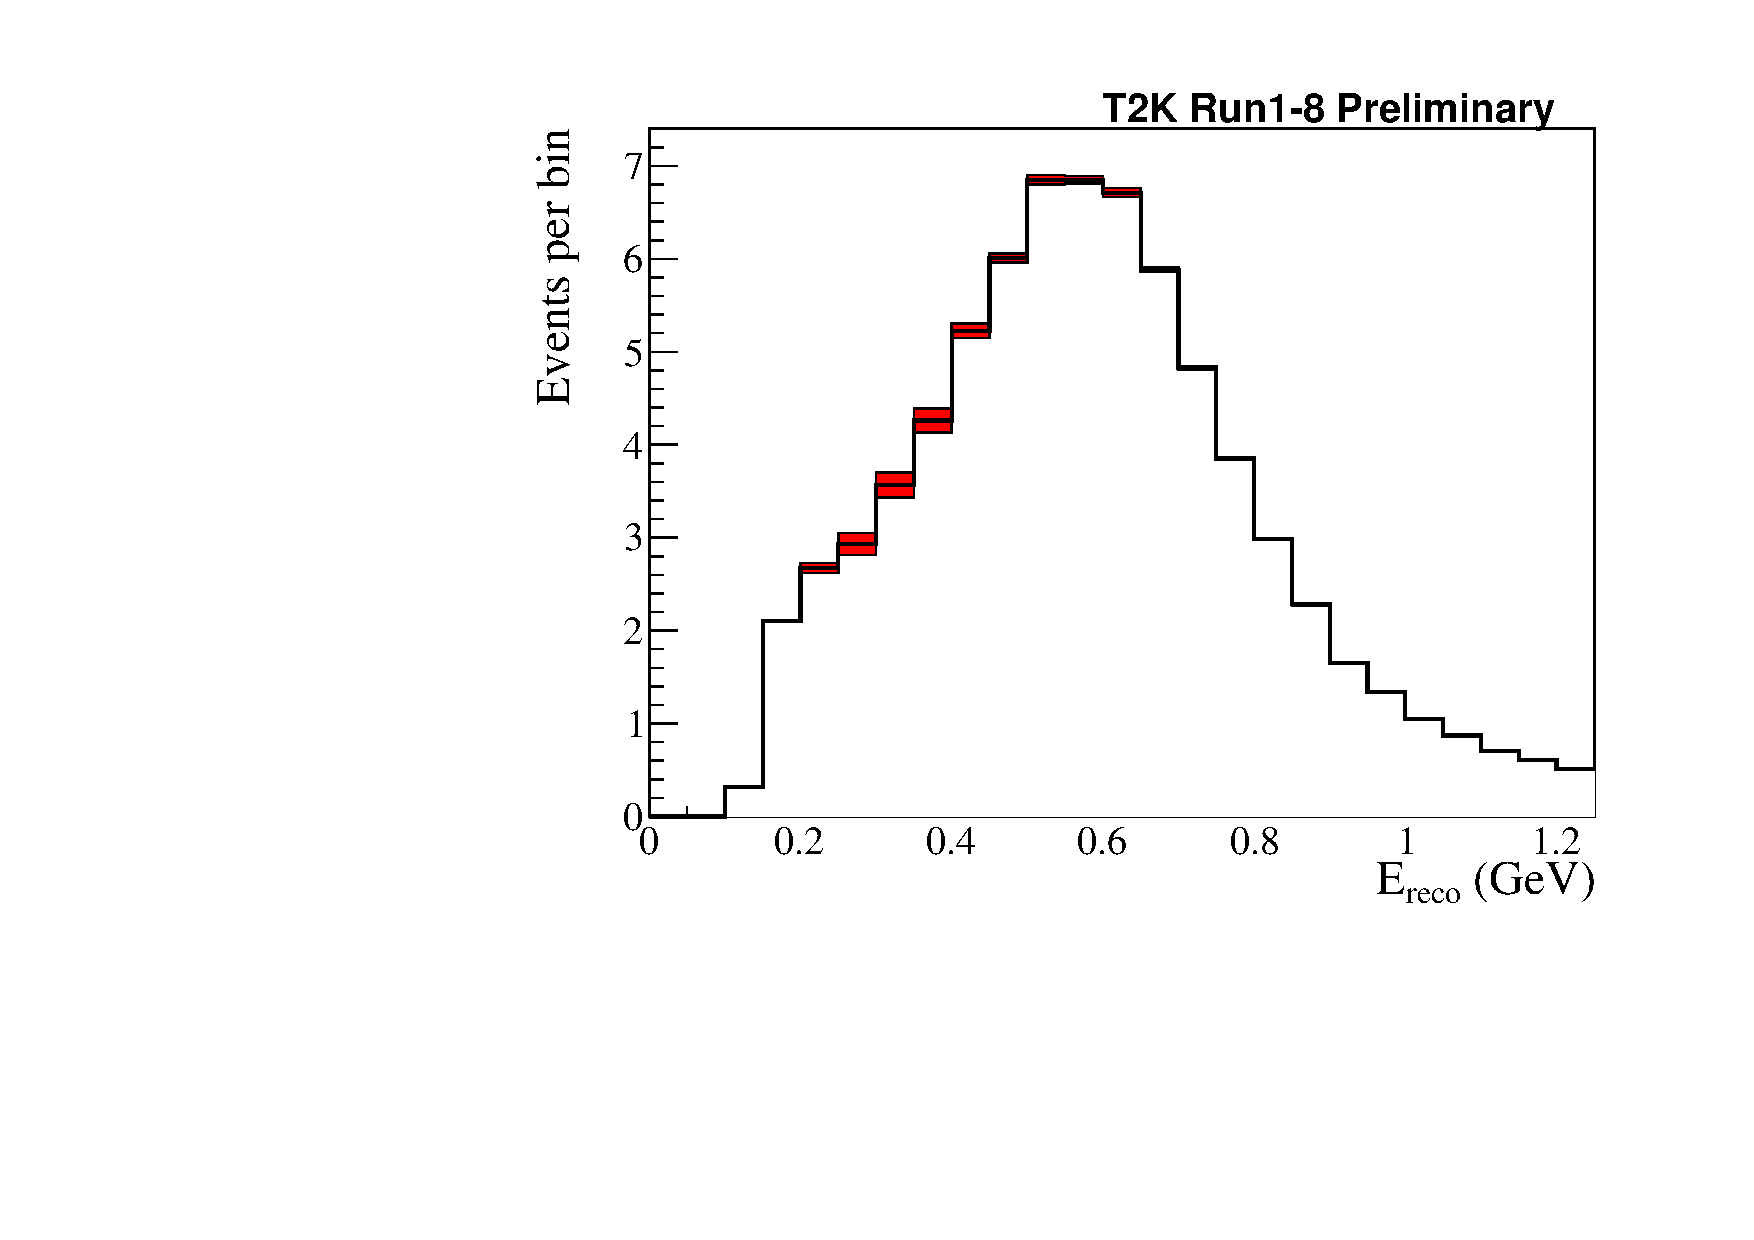
\includegraphics[width=0.9\textwidth]{images/systematics/envelopes/sk_error_table_1Re_xsec_ncgamma_envelope}
		\caption{Electron-like, neutrino mode}
	\end{subfigure}
	\begin{subfigure}[b]{0.49\textwidth}
		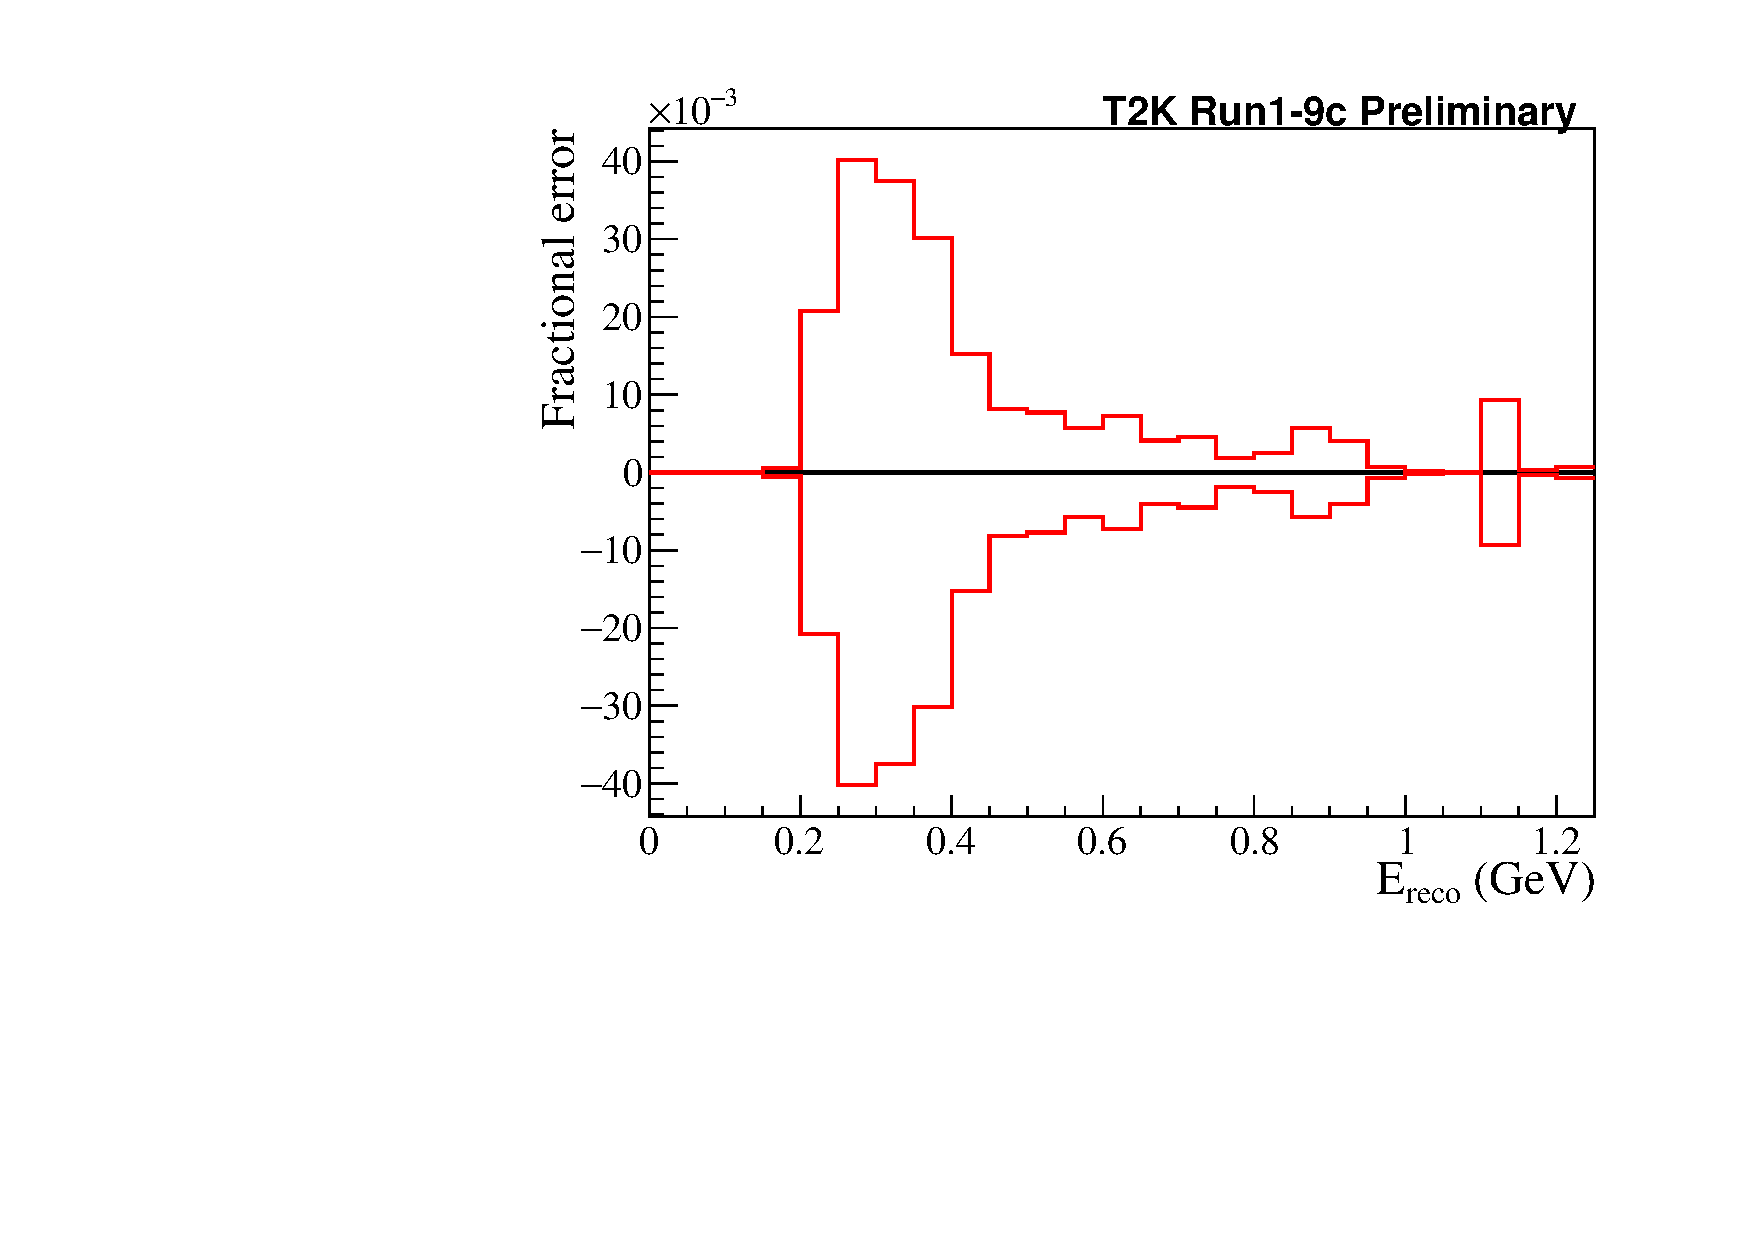
\includegraphics[width=0.9\textwidth]{images/systematics/envelopes/sk_error_table_1Re_xsec_ncgamma_envelope_fractional}
		\caption{Electron-like, neutrino mode}
	\end{subfigure}
	\begin{subfigure}[b]{0.49\textwidth}
		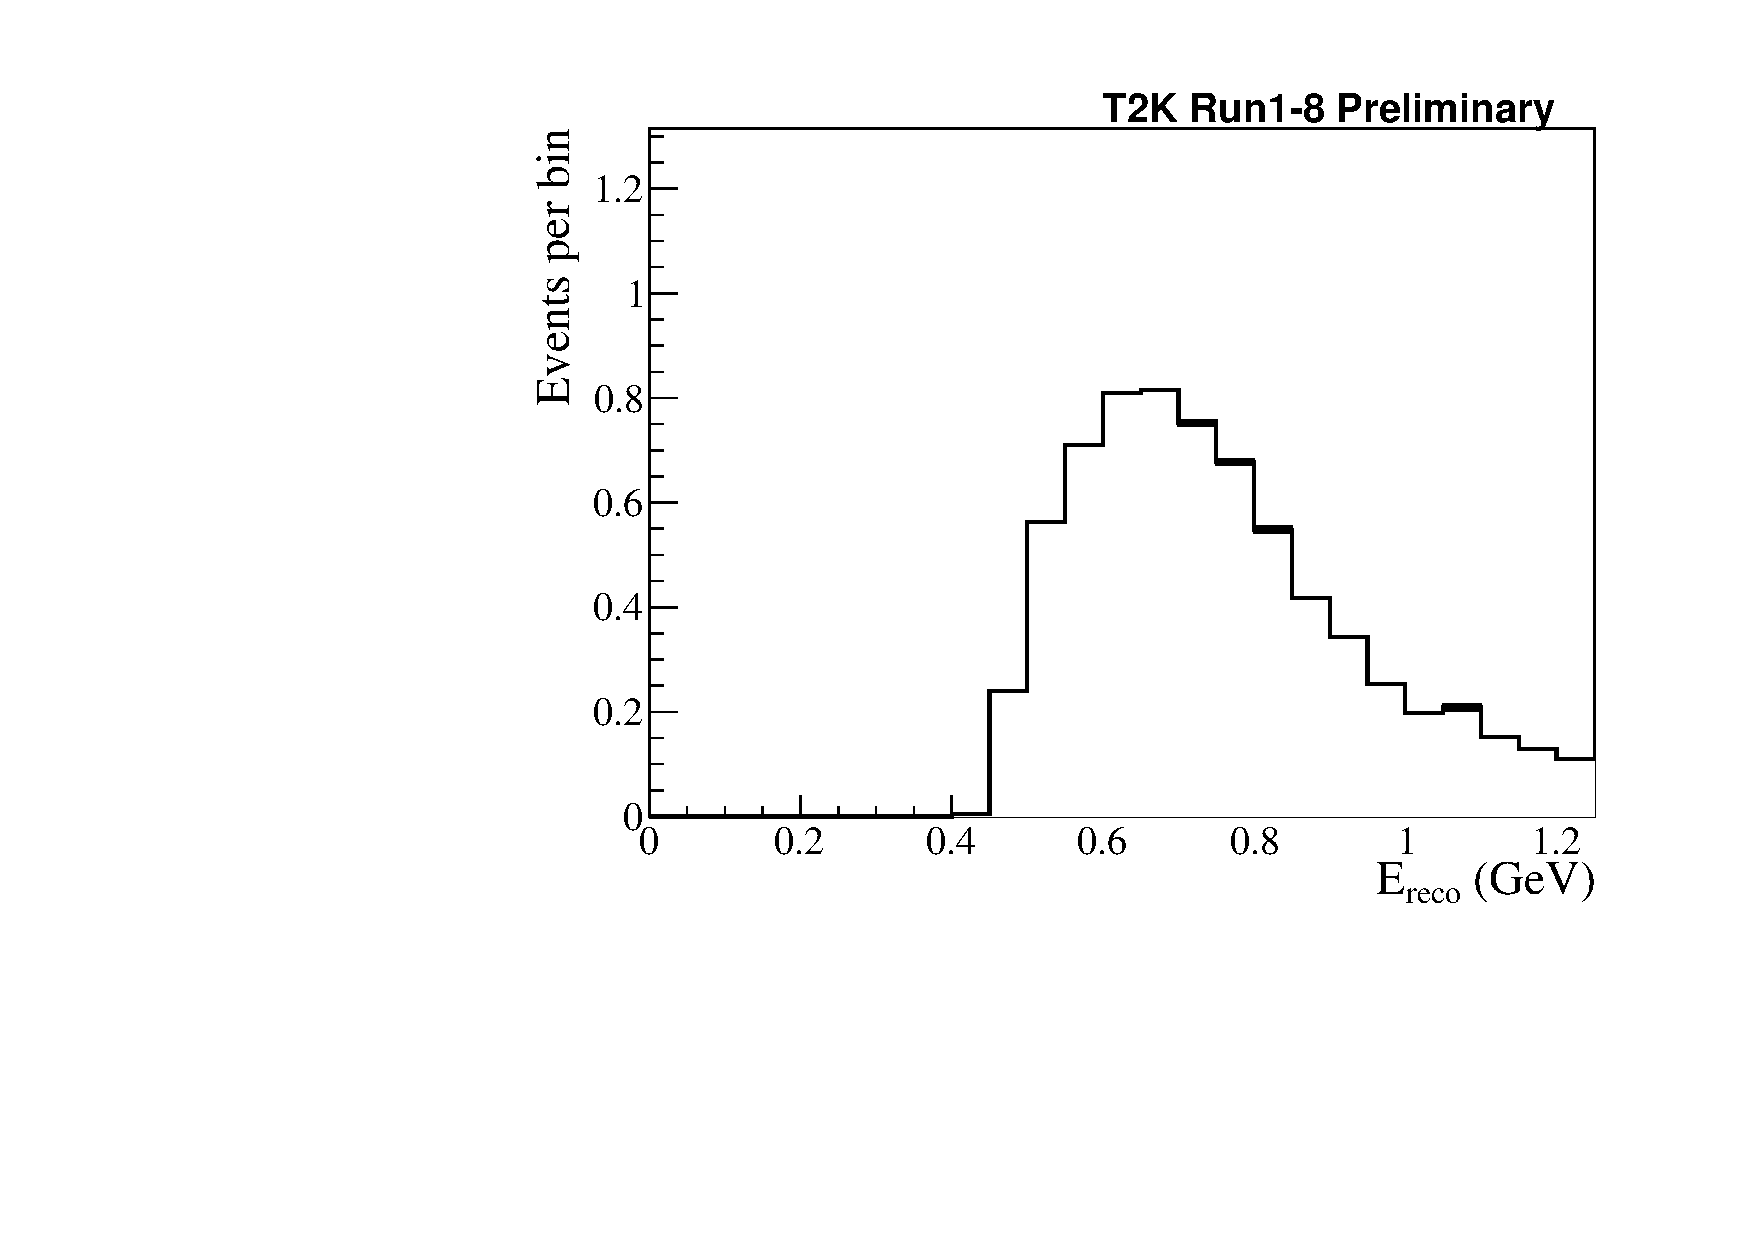
\includegraphics[width=0.9\textwidth]{images/systematics/envelopes/sk_error_table_MultiRe_xsec_ncgamma_envelope}
		\caption{\nueCConepi-like, neutrino mode}
	\end{subfigure}
	\begin{subfigure}[b]{0.49\textwidth}
		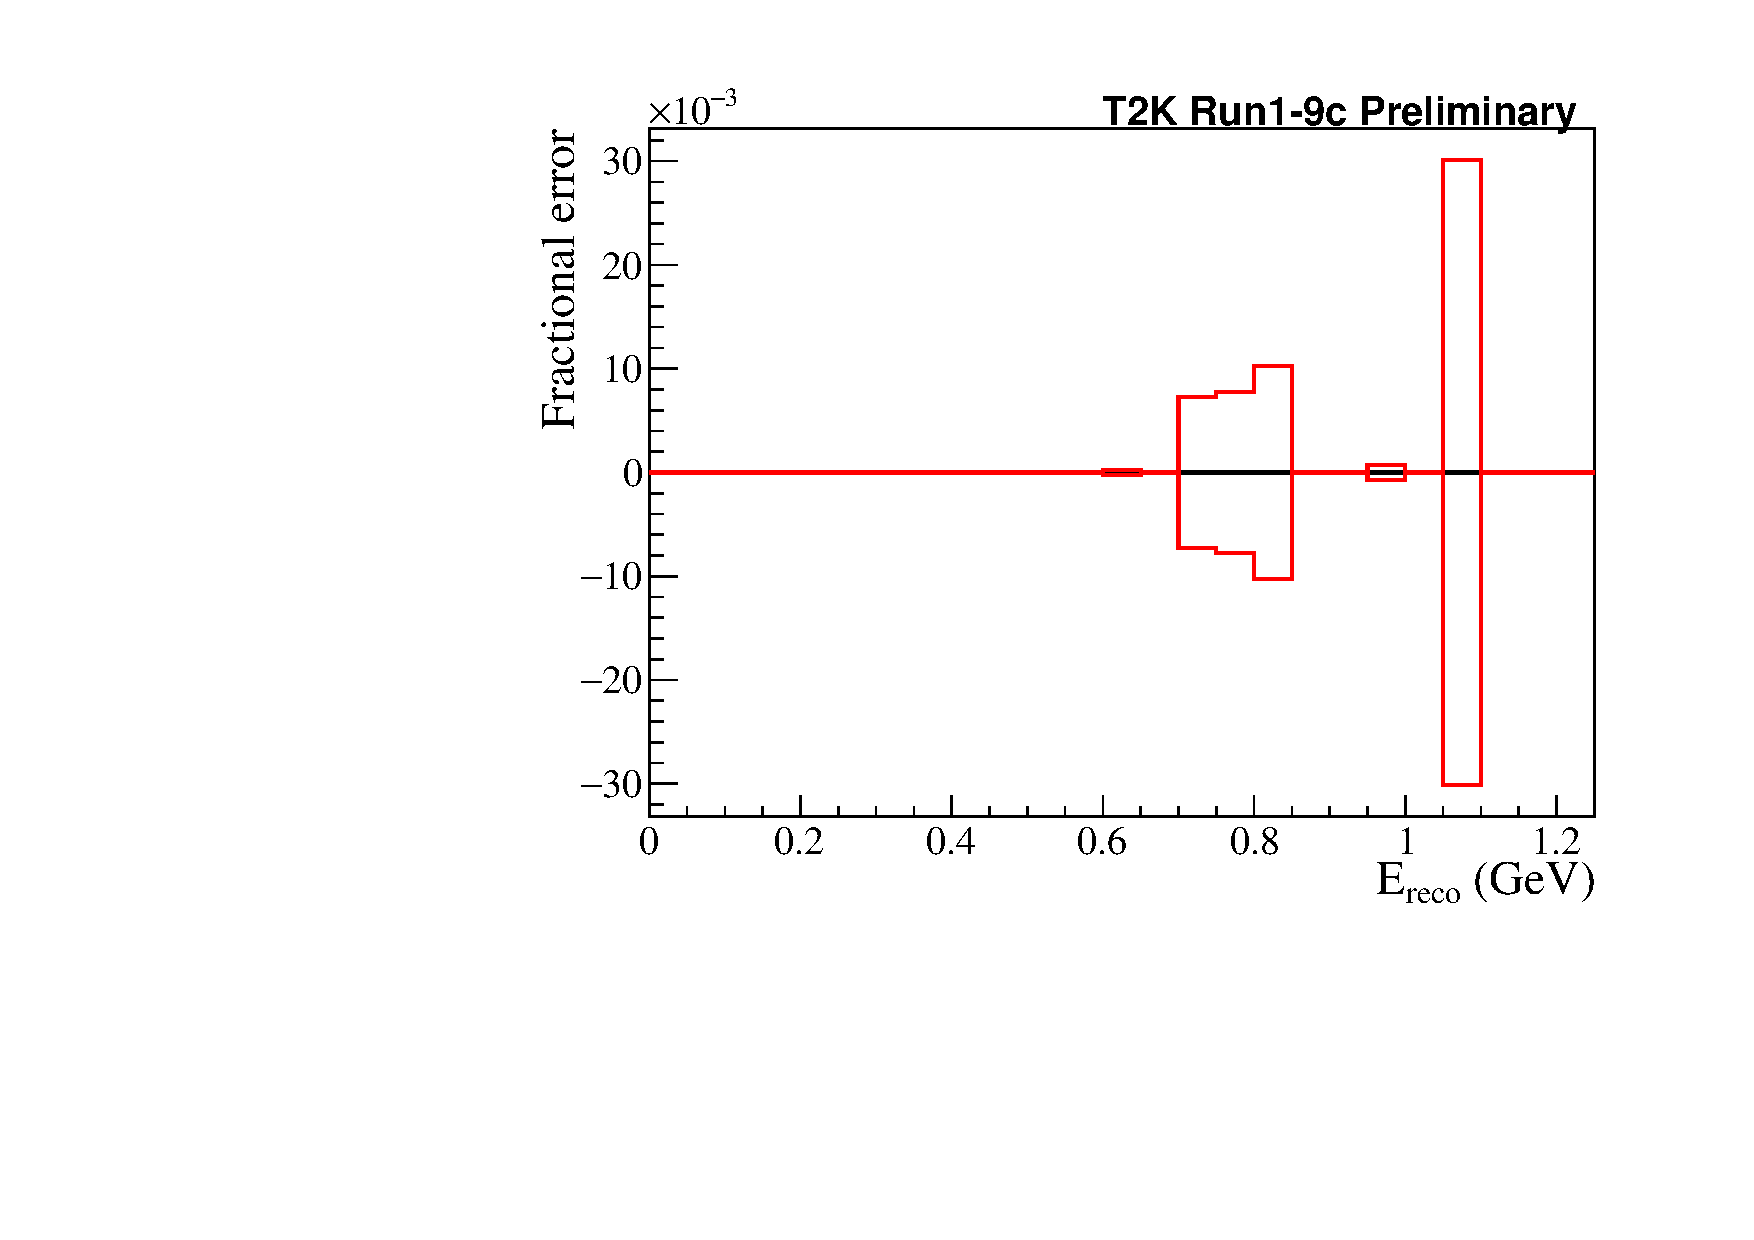
\includegraphics[width=0.9\textwidth]{images/systematics/envelopes/sk_error_table_MultiRe_xsec_ncgamma_envelope_fractional}
		\caption{\nueCConepi-like, neutrino mode}
	\end{subfigure}
	\caption {
		Error envelopes (left) and fractional error (right) for the reconstructed neutrino energy spectrum for the unconstrained NC$1\gamma$ systematic parameters. \NumToysSmall toys are generated for the Asimov data set A with randomized systematic parameters with correlations taken into account.
	}
	\label{fig:sk_envelopes_xsec_ncgamma}
\end{figure*}
\clearpage

\begin{figure*}
	\center
	\begin{subfigure}[b]{0.49\textwidth}
		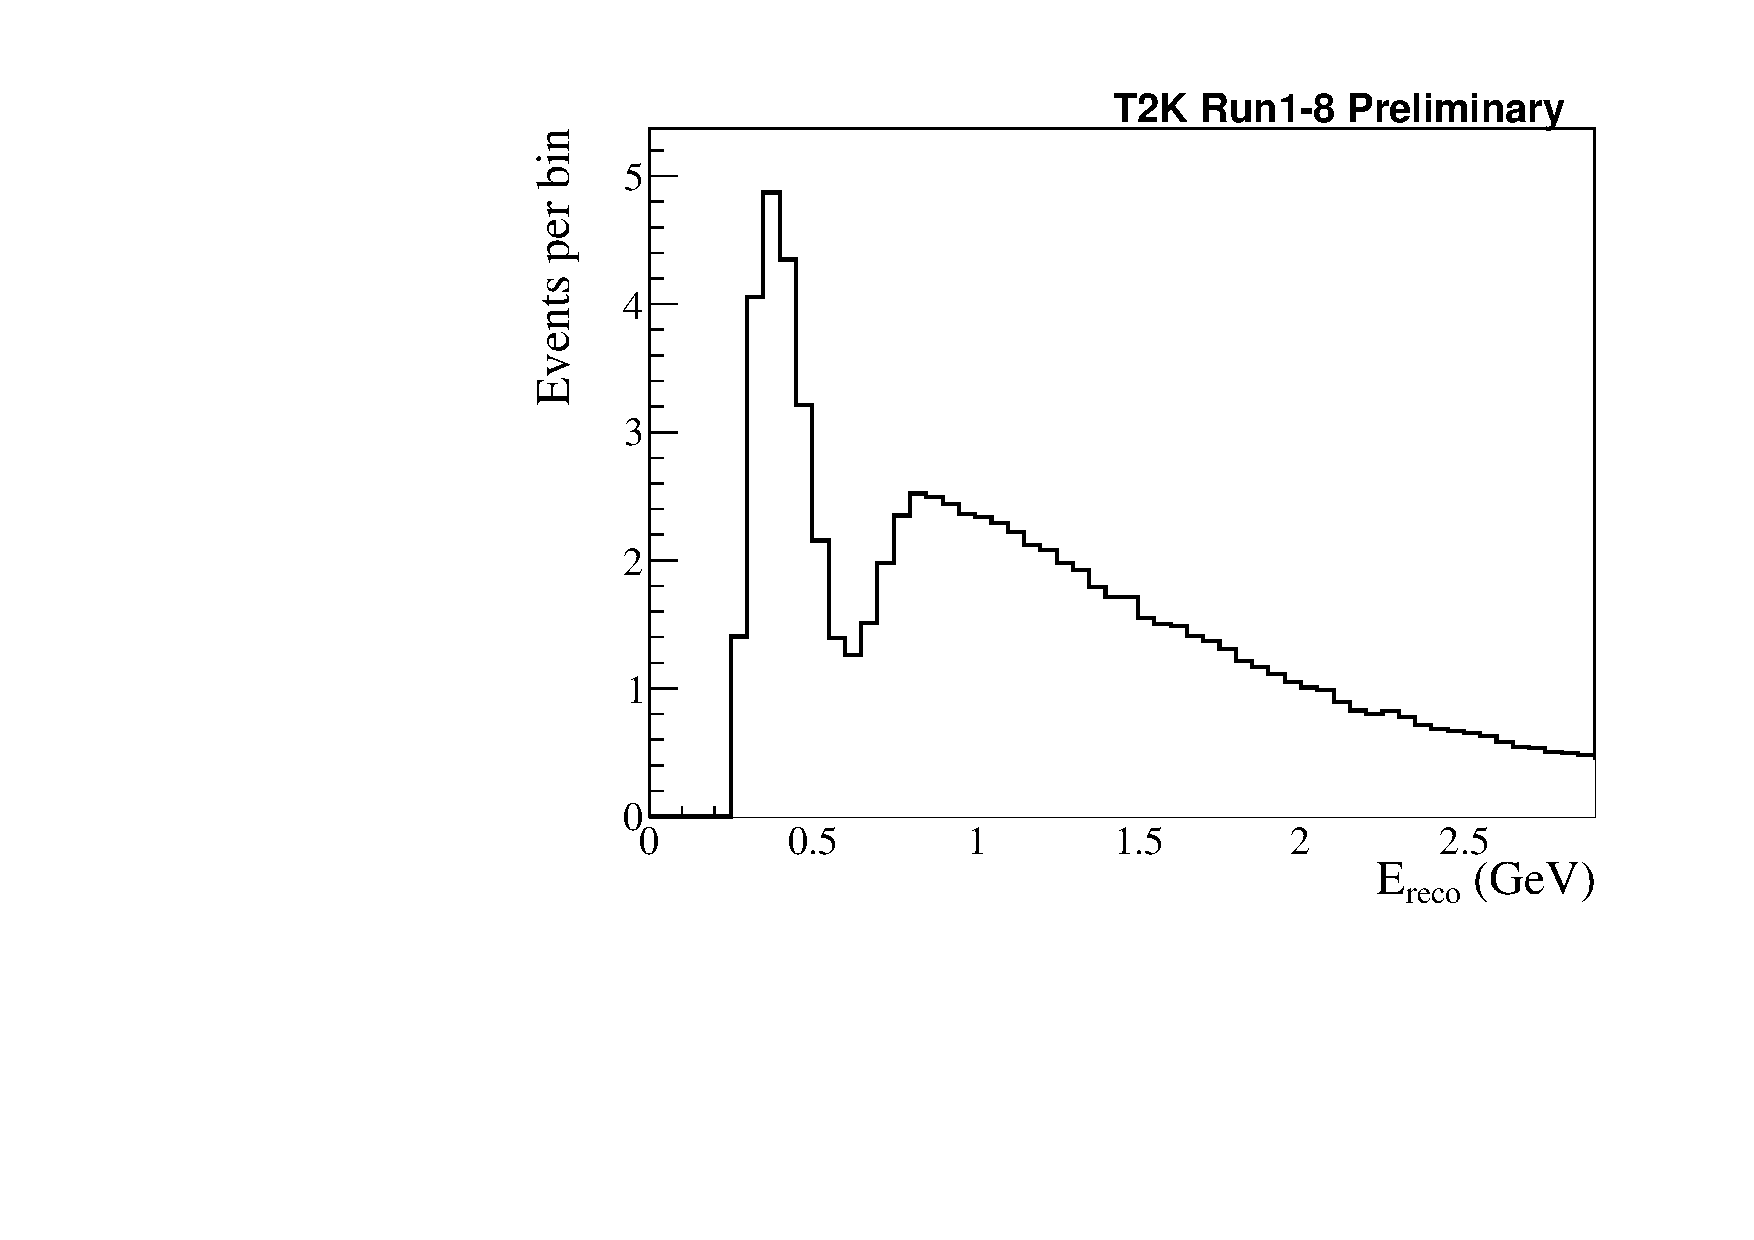
\includegraphics[width=0.9\textwidth]{images/systematics/envelopes/sk_error_table_RHC1Rmu_xsec_ncgamma_envelope}
		\caption{Muon-like, antineutrino mode}
	\end{subfigure}
	\begin{subfigure}[b]{0.49\textwidth}
		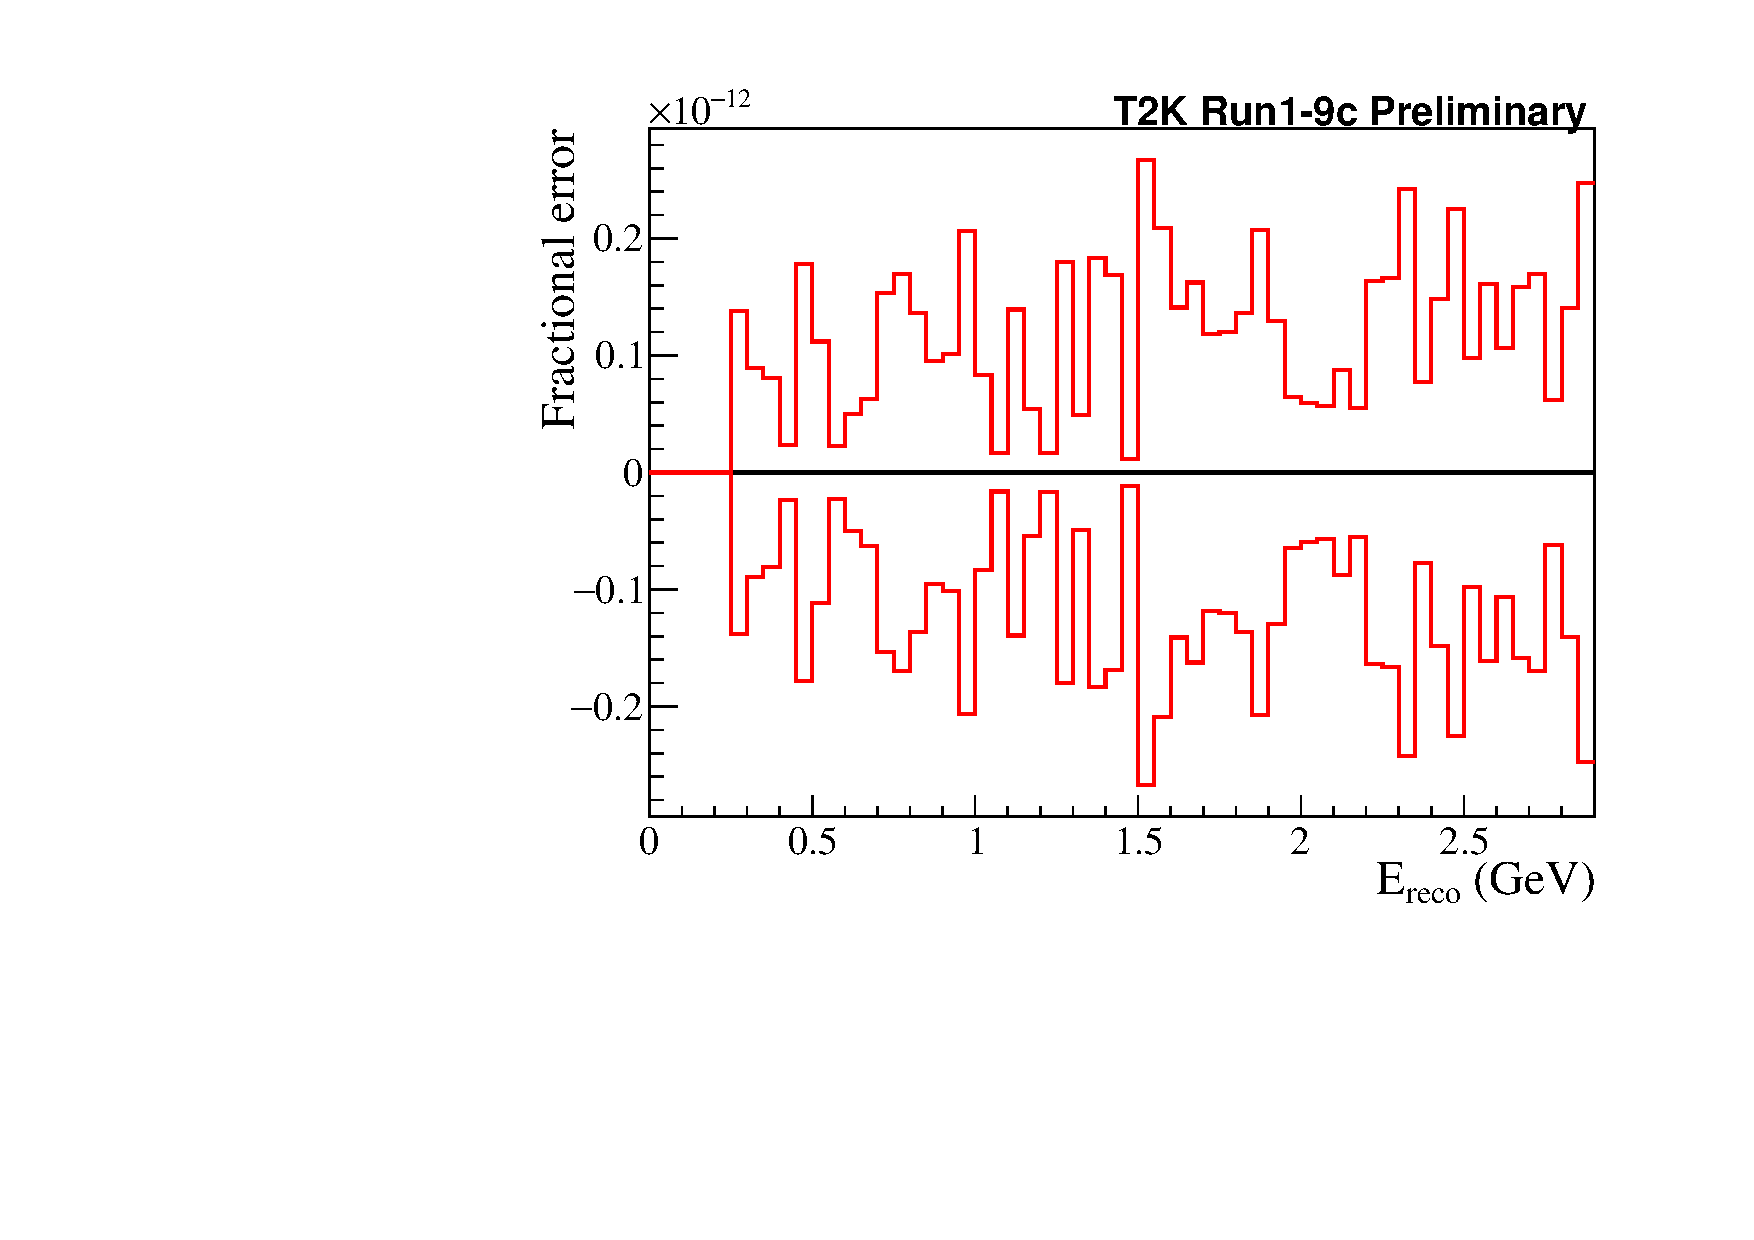
\includegraphics[width=0.9\textwidth]{images/systematics/envelopes/sk_error_table_RHC1Rmu_xsec_ncgamma_envelope_fractional}
		\caption{Muon-like, antineutrino mode}
	\end{subfigure}
	\begin{subfigure}[b]{0.49\textwidth}
		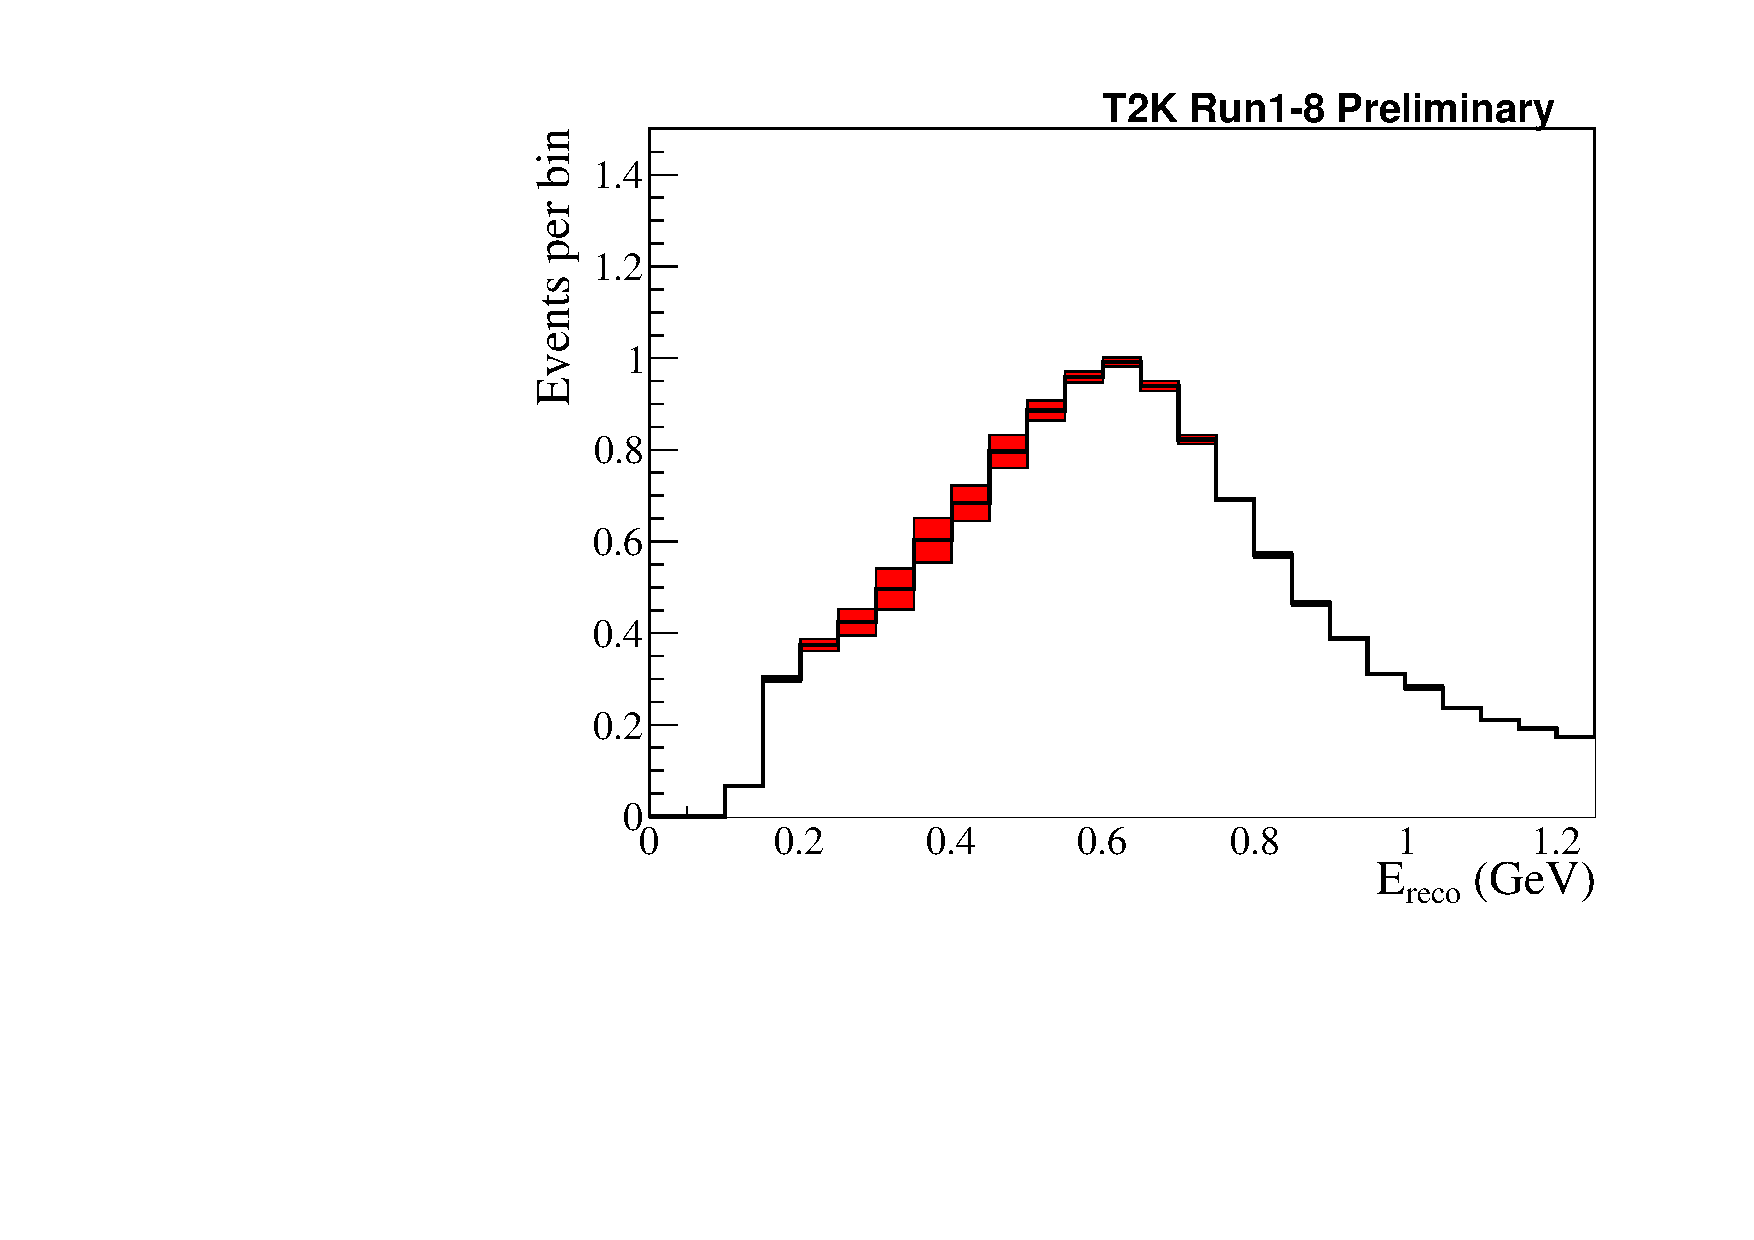
\includegraphics[width=0.9\textwidth]{images/systematics/envelopes/sk_error_table_RHC1Re_xsec_ncgamma_envelope}
		\caption{Electron-like antineutrino mode}
	\end{subfigure}
	\begin{subfigure}[b]{0.49\textwidth}
		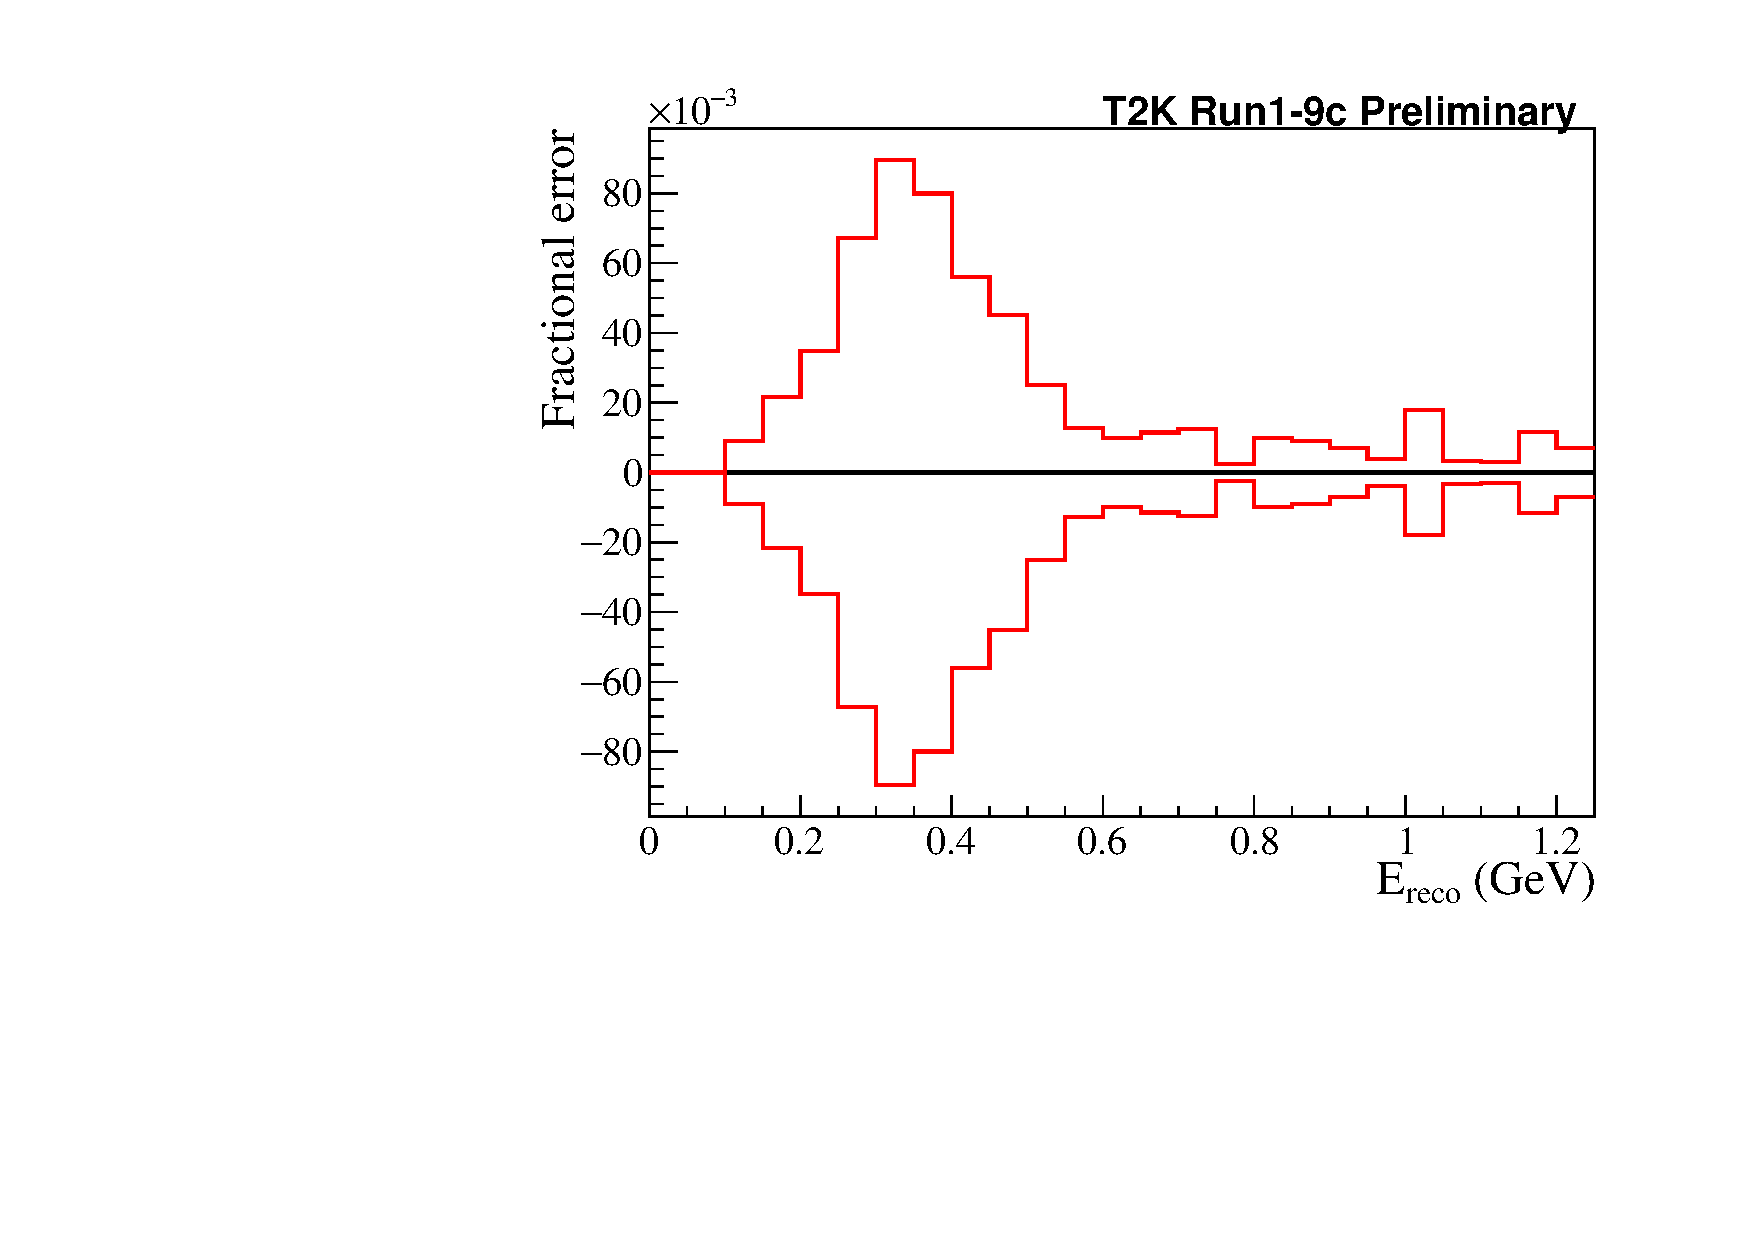
\includegraphics[width=0.9\textwidth]{images/systematics/envelopes/sk_error_table_RHC1Re_xsec_ncgamma_envelope_fractional}
		\caption{Electron-like antineutrino mode}
	\end{subfigure}
	\caption {
		Error envelopes (left) and fractional errors (right) for the reconstructed neutrino energy spectrum for the unconstrained NC$1\gamma$ systematic parameters. \NumToysSmall toys are generated for the Asimov data set A with randomized systematic parameters with correlations taken into account.
	}
	\label{fig:sk_envelopes_xsec_ncgamma_b}
\end{figure*}
\clearpage
\begin{figure*}
	\center
	\begin{subfigure}[b]{0.49\textwidth}
		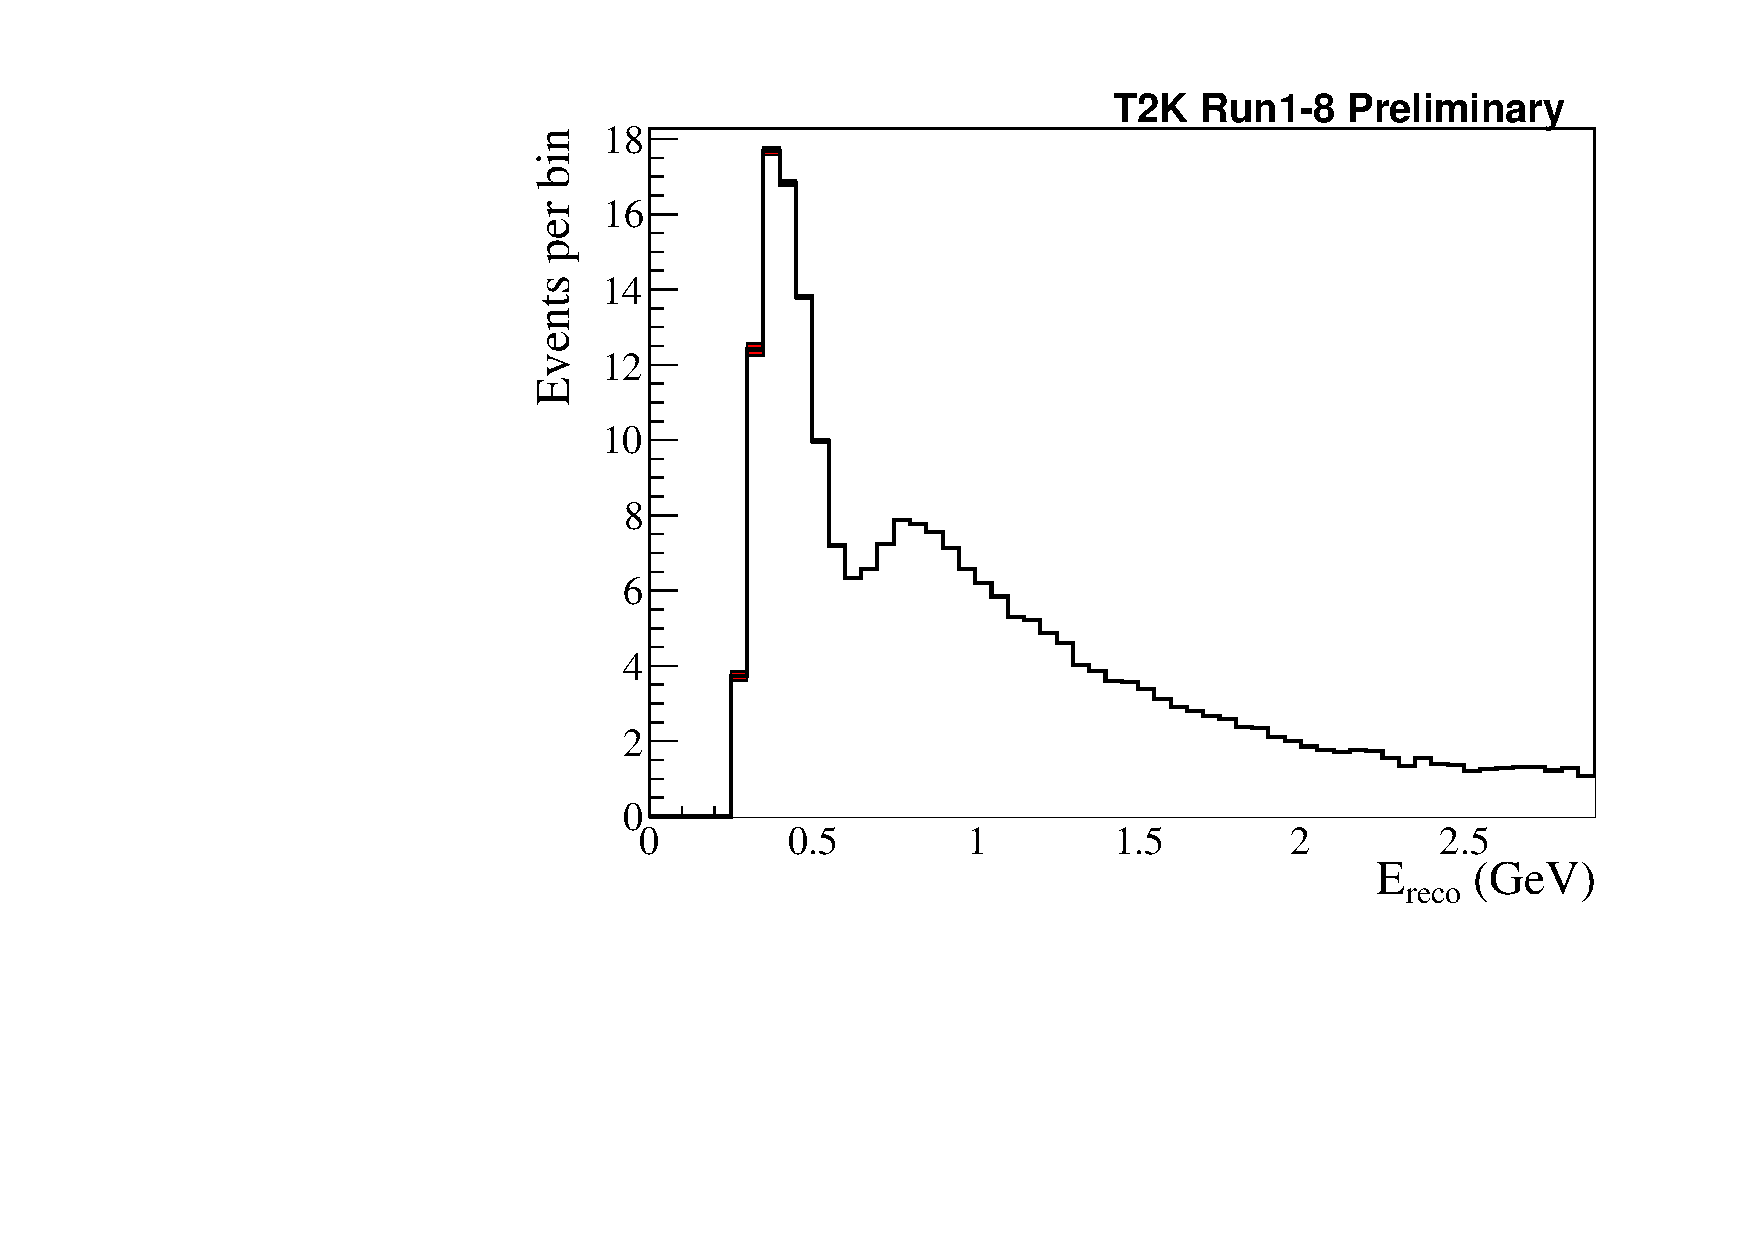
\includegraphics[width=0.9\textwidth]{images/systematics/envelopes/sk_error_table_1Rmu_xsec_ncoth_envelope}
		\caption{Muon-like, neutrino mode}
	\end{subfigure}
	\begin{subfigure}[b]{0.49\textwidth}
		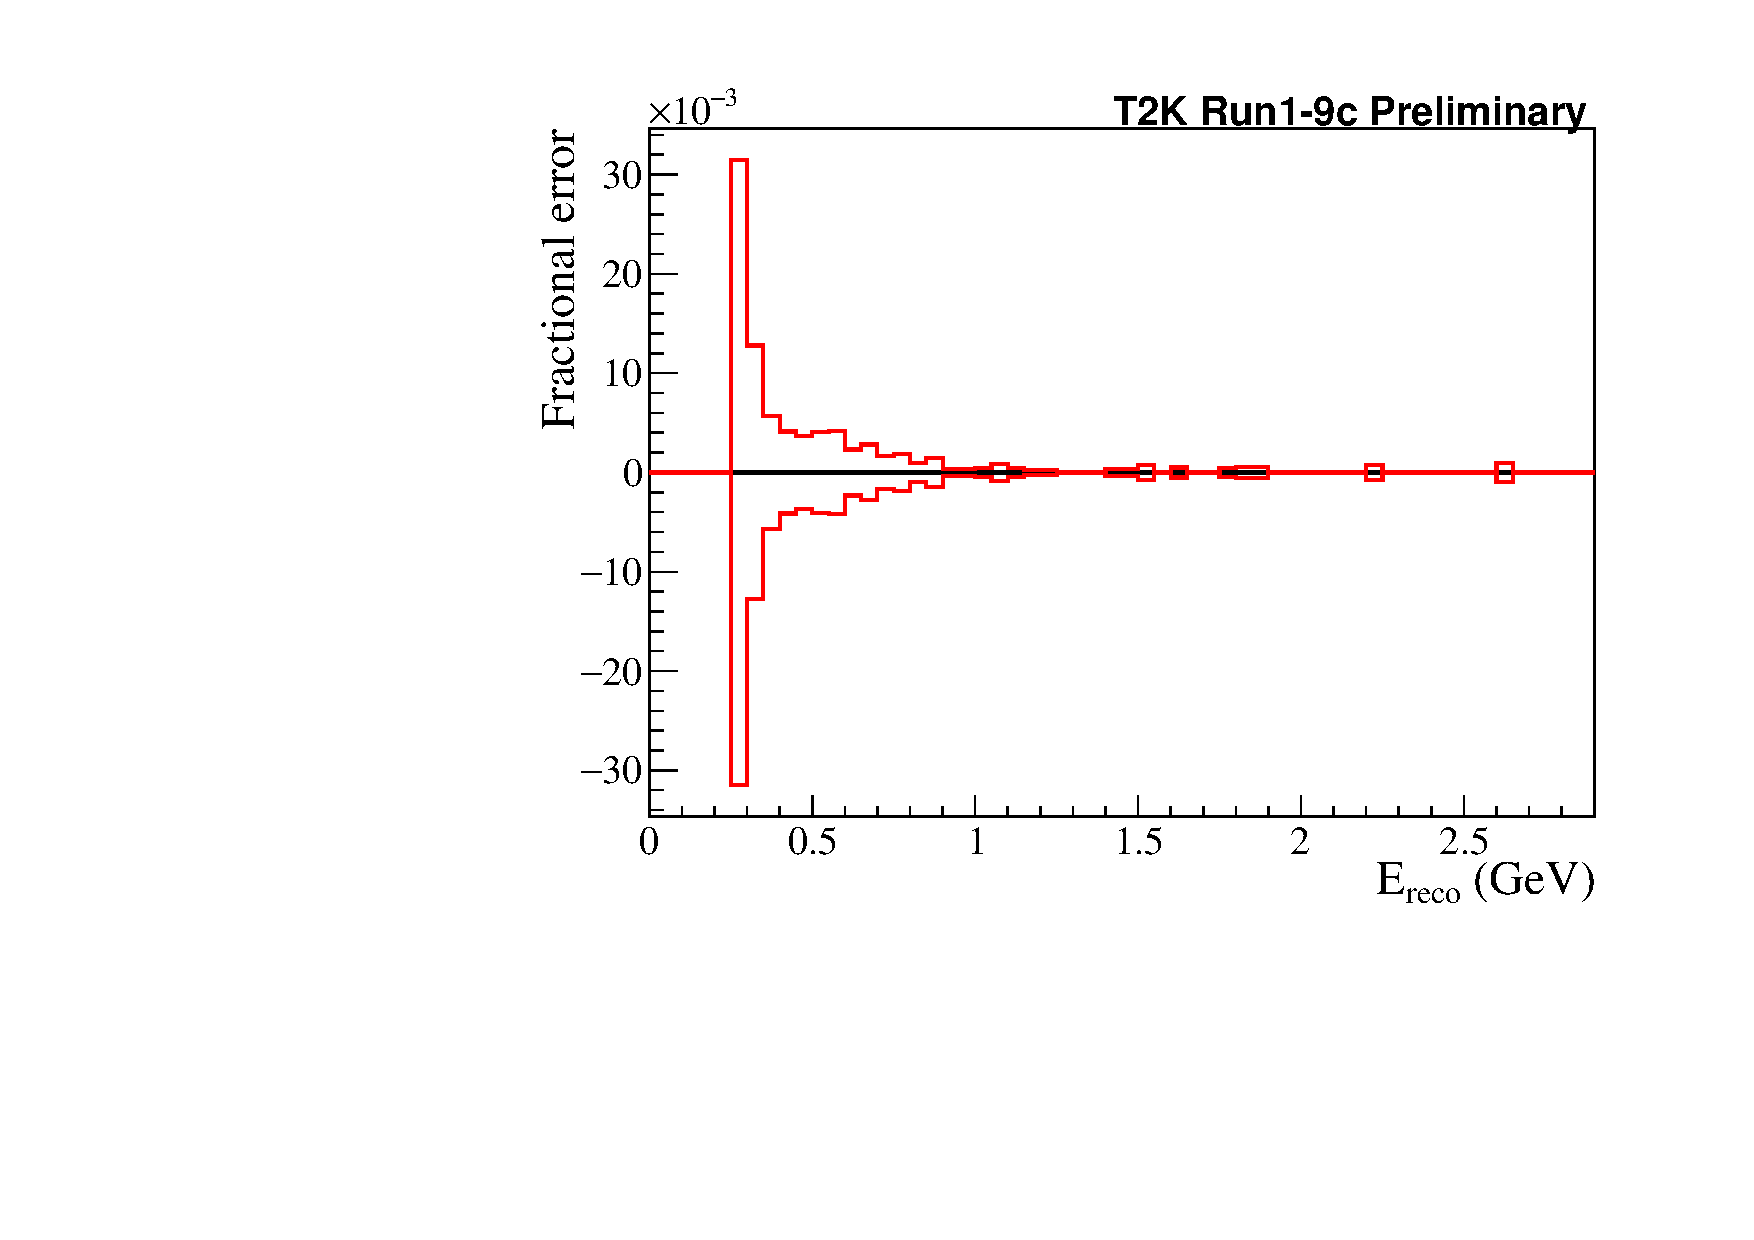
\includegraphics[width=0.9\textwidth]{images/systematics/envelopes/sk_error_table_1Rmu_xsec_ncoth_envelope_fractional}
		\caption{Muon-like, neutrino mode}
	\end{subfigure}
	\begin{subfigure}[b]{0.49\textwidth}
		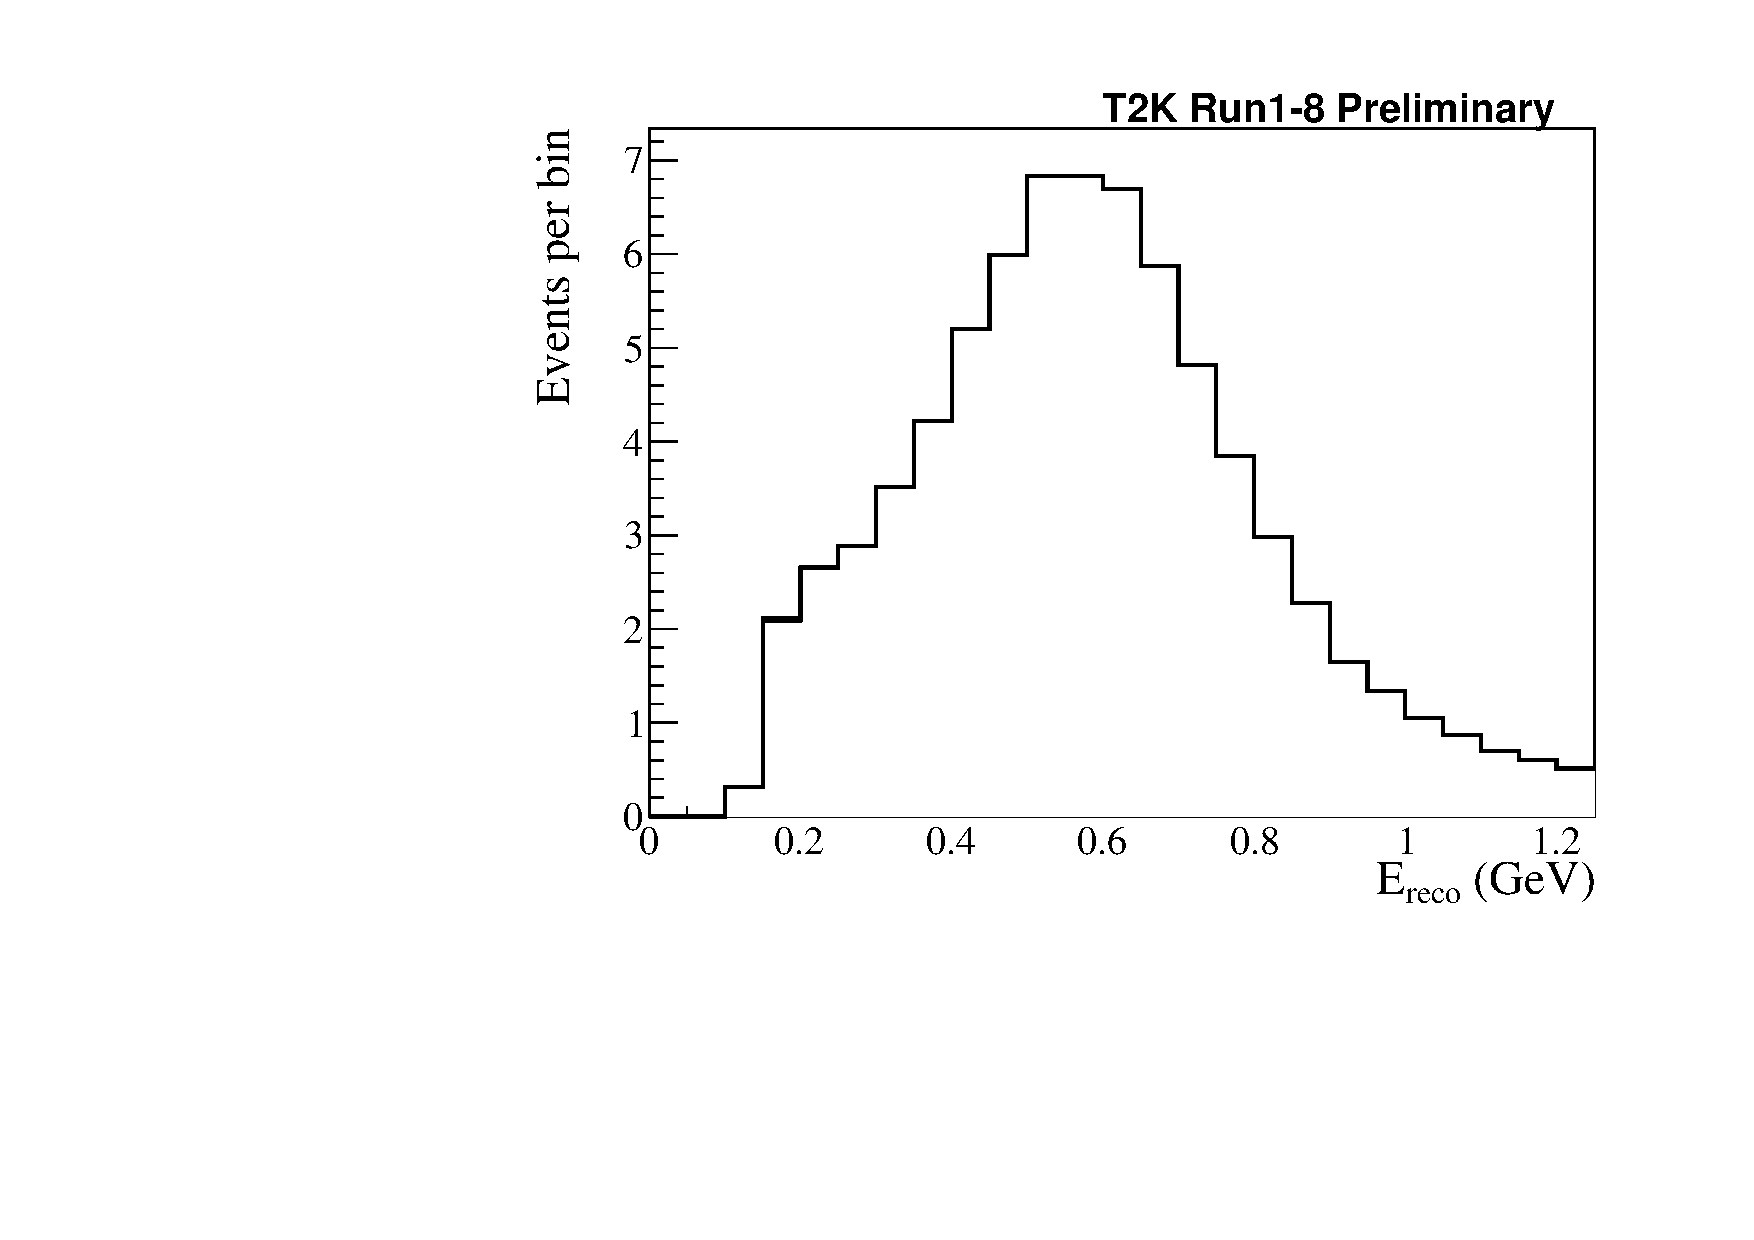
\includegraphics[width=0.9\textwidth]{images/systematics/envelopes/sk_error_table_1Re_xsec_ncoth_envelope}
		\caption{Electron-like, neutrino mode}
	\end{subfigure}
	\begin{subfigure}[b]{0.49\textwidth}
		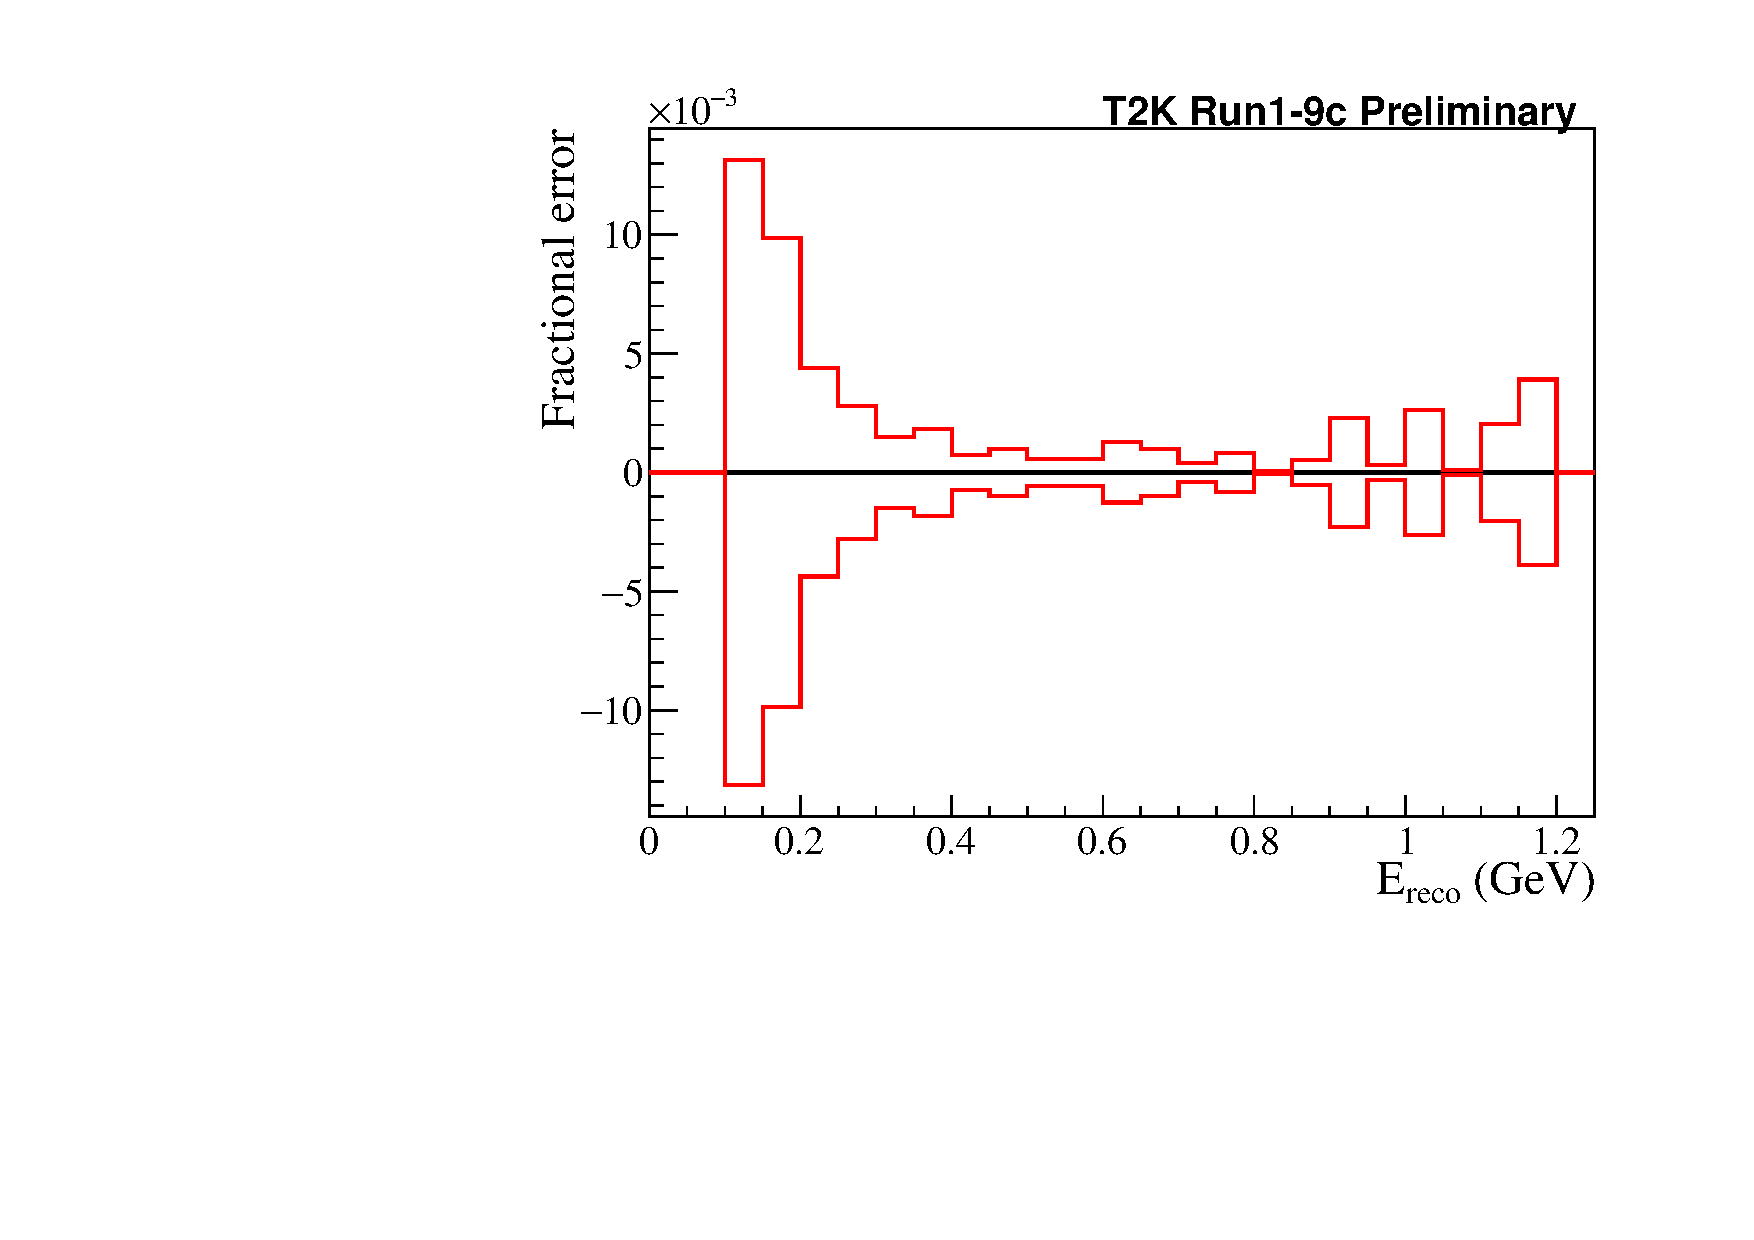
\includegraphics[width=0.9\textwidth]{images/systematics/envelopes/sk_error_table_1Re_xsec_ncoth_envelope_fractional}
		\caption{Electron-like, neutrino mode}
	\end{subfigure}
	\begin{subfigure}[b]{0.49\textwidth}
		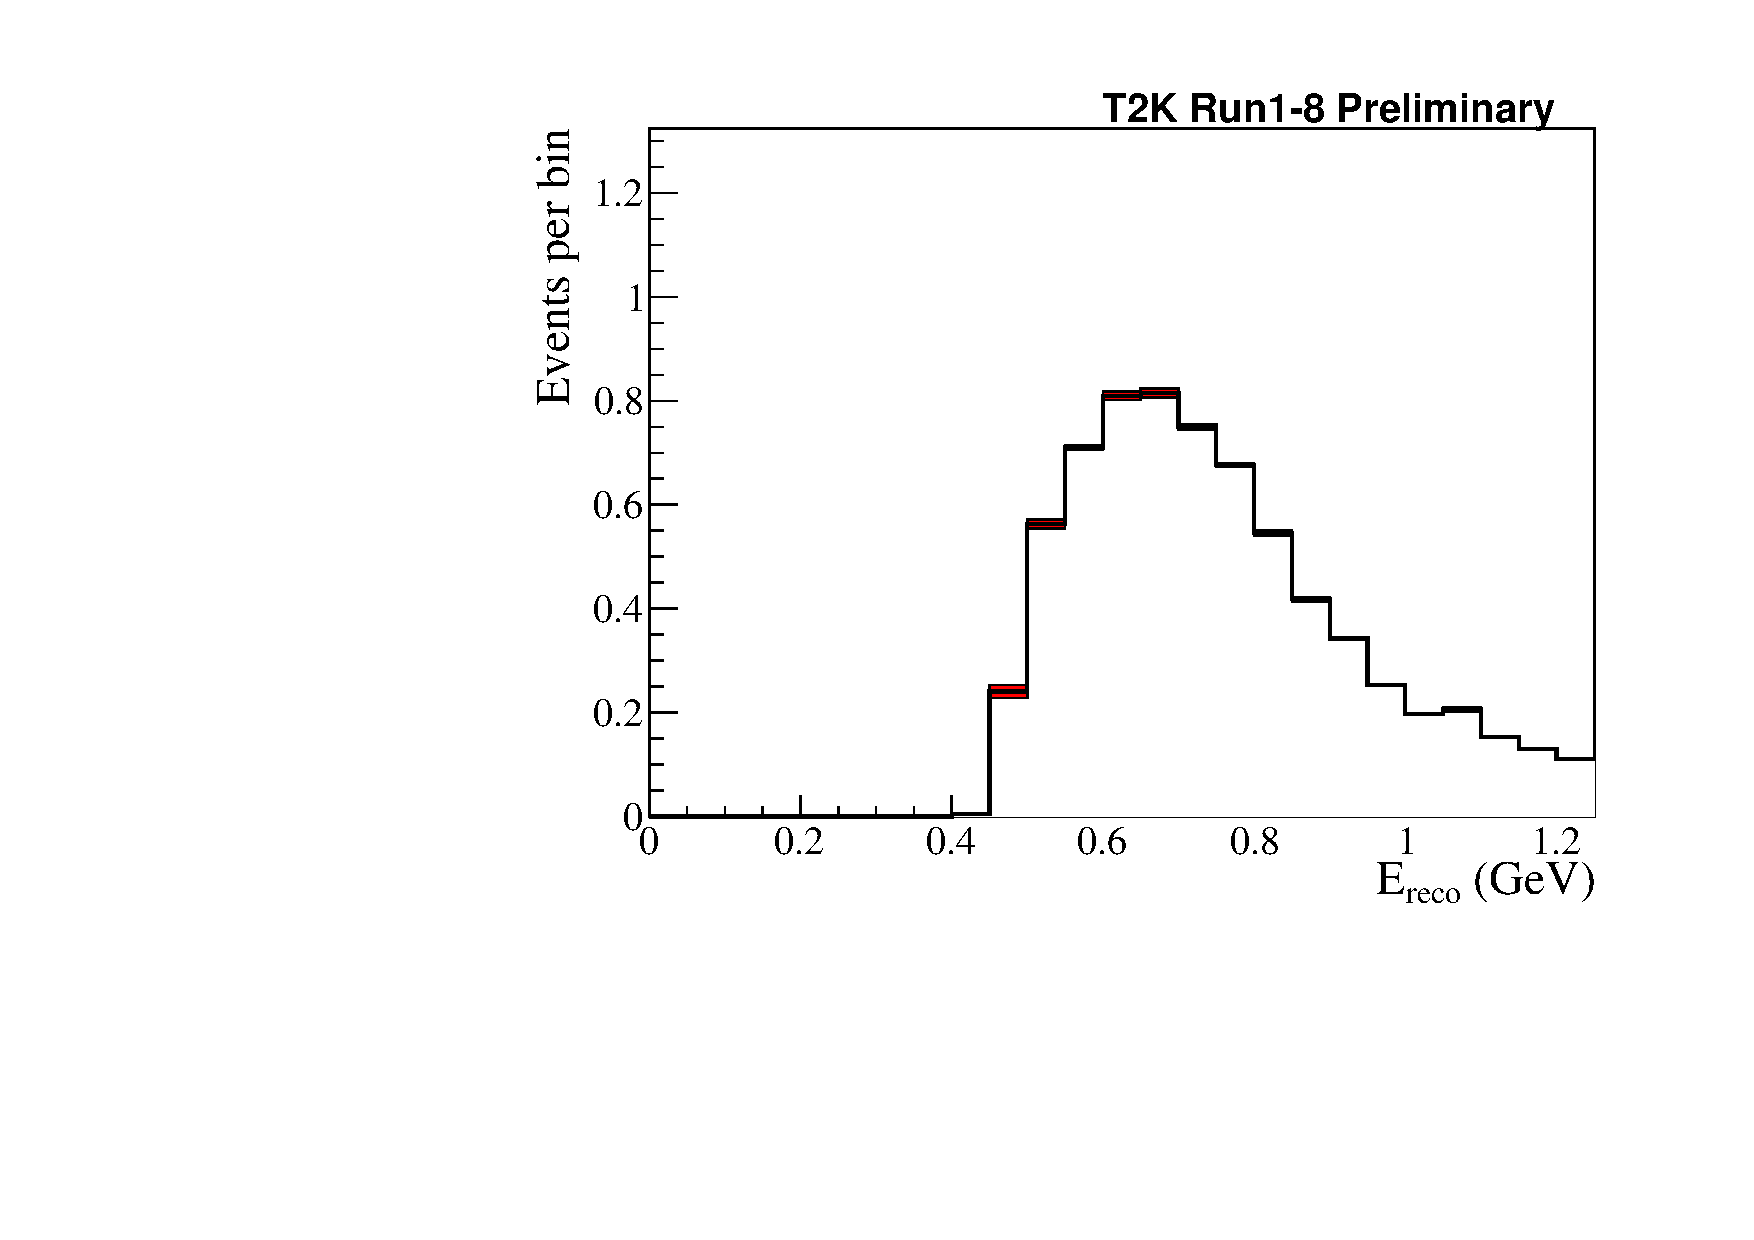
\includegraphics[width=0.9\textwidth]{images/systematics/envelopes/sk_error_table_MultiRe_xsec_ncoth_envelope}
		\caption{\nueCConepi-like, neutrino mode}
	\end{subfigure}
	\begin{subfigure}[b]{0.49\textwidth}
		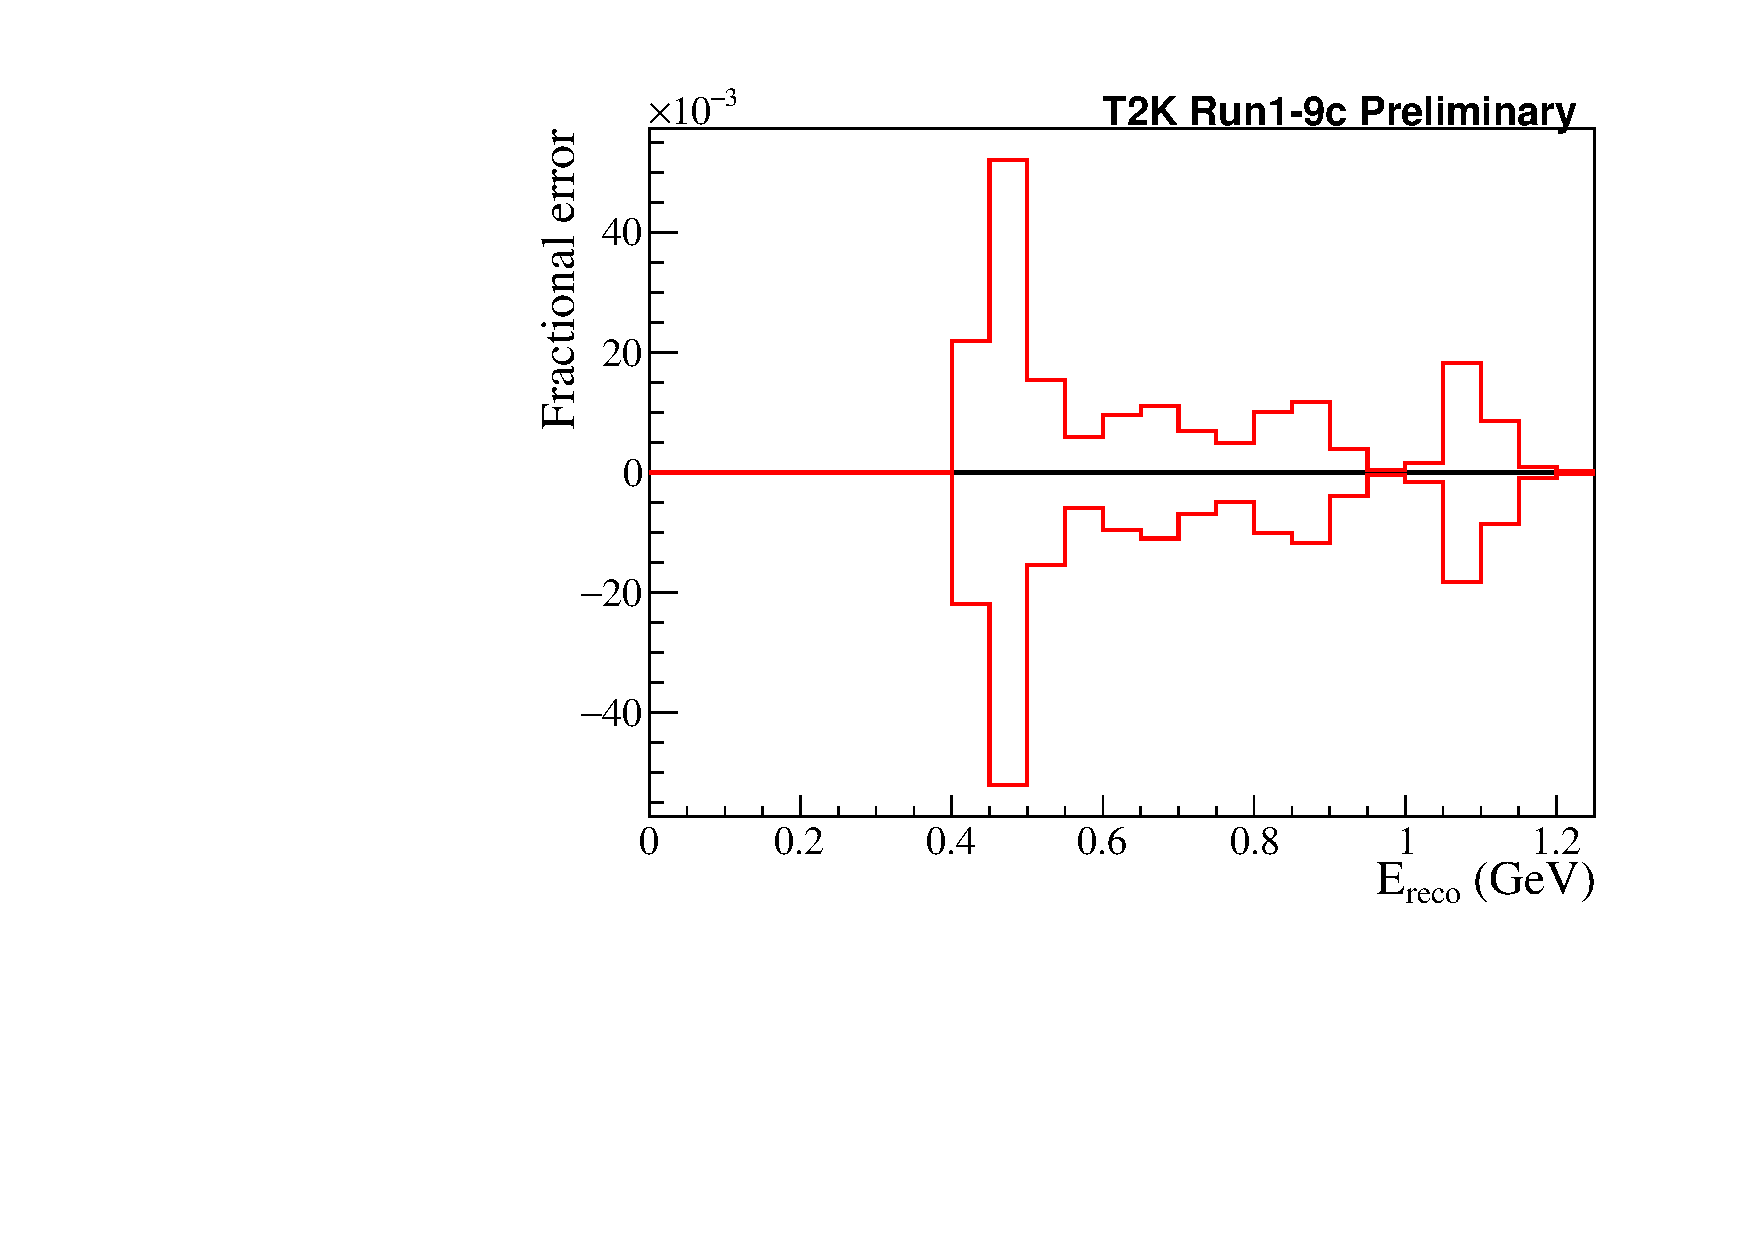
\includegraphics[width=0.9\textwidth]{images/systematics/envelopes/sk_error_table_MultiRe_xsec_ncoth_envelope_fractional}
		\caption{\nueCConepi-like, neutrino mode}
	\end{subfigure}
	\caption {
		Error envelopes (left) and fractional errors (right) for the reconstructed neutrino energy spectrum for the unconstrained NCother systematic parameters. \NumToysSmall toys are generated for the Asimov data set A with randomized systematic parameters with correlations taken into account.
	}
	\label{fig:sk_envelopes_xsec_ncoth}
\end{figure*}
\clearpage

\begin{figure*}
	\center
	\begin{subfigure}[b]{0.49\textwidth}
		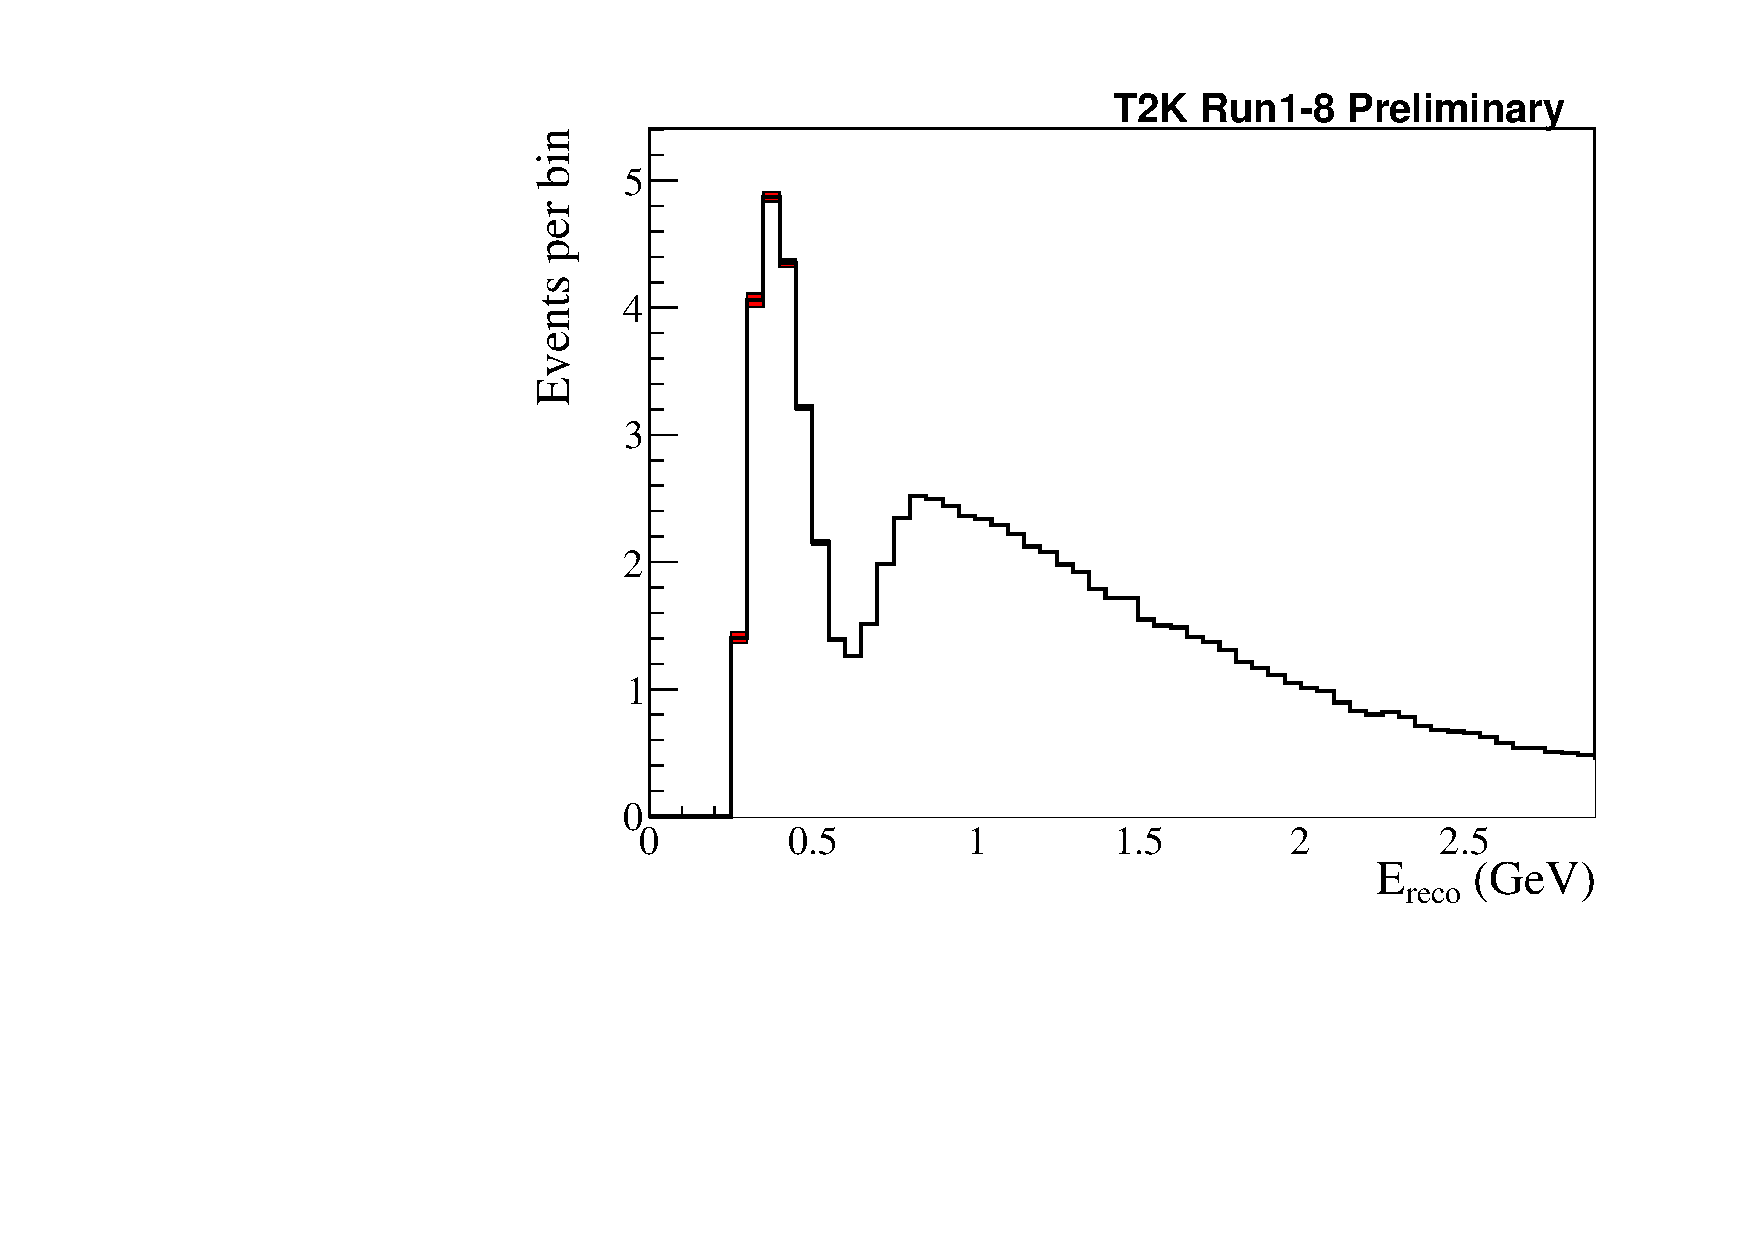
\includegraphics[width=0.9\textwidth]{images/systematics/envelopes/sk_error_table_RHC1Rmu_xsec_ncoth_envelope}
		\caption{Muon-like, antineutrino mode}
	\end{subfigure}
	\begin{subfigure}[b]{0.49\textwidth}
		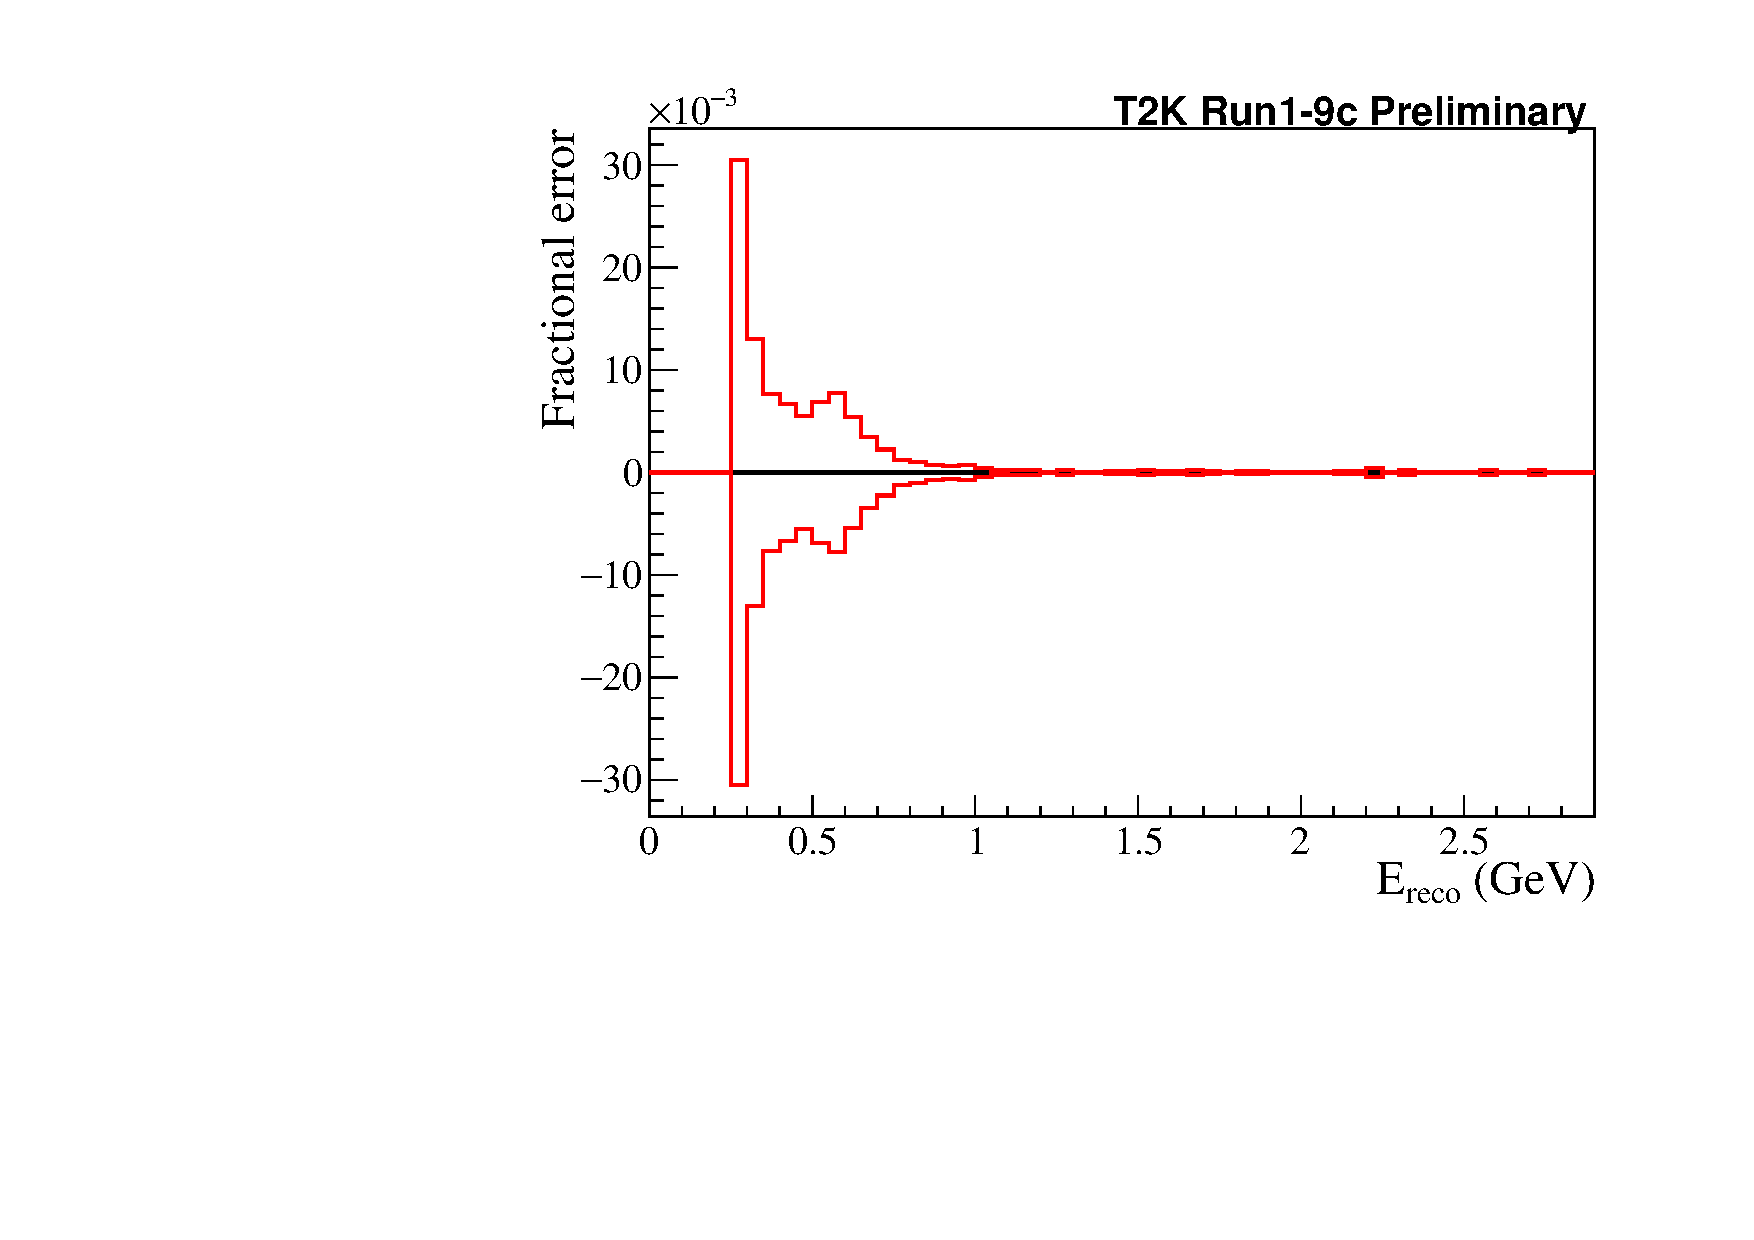
\includegraphics[width=0.9\textwidth]{images/systematics/envelopes/sk_error_table_RHC1Rmu_xsec_ncoth_envelope_fractional}
		\caption{Muon-like, antineutrino mode}
	\end{subfigure}
	\begin{subfigure}[b]{0.49\textwidth}
		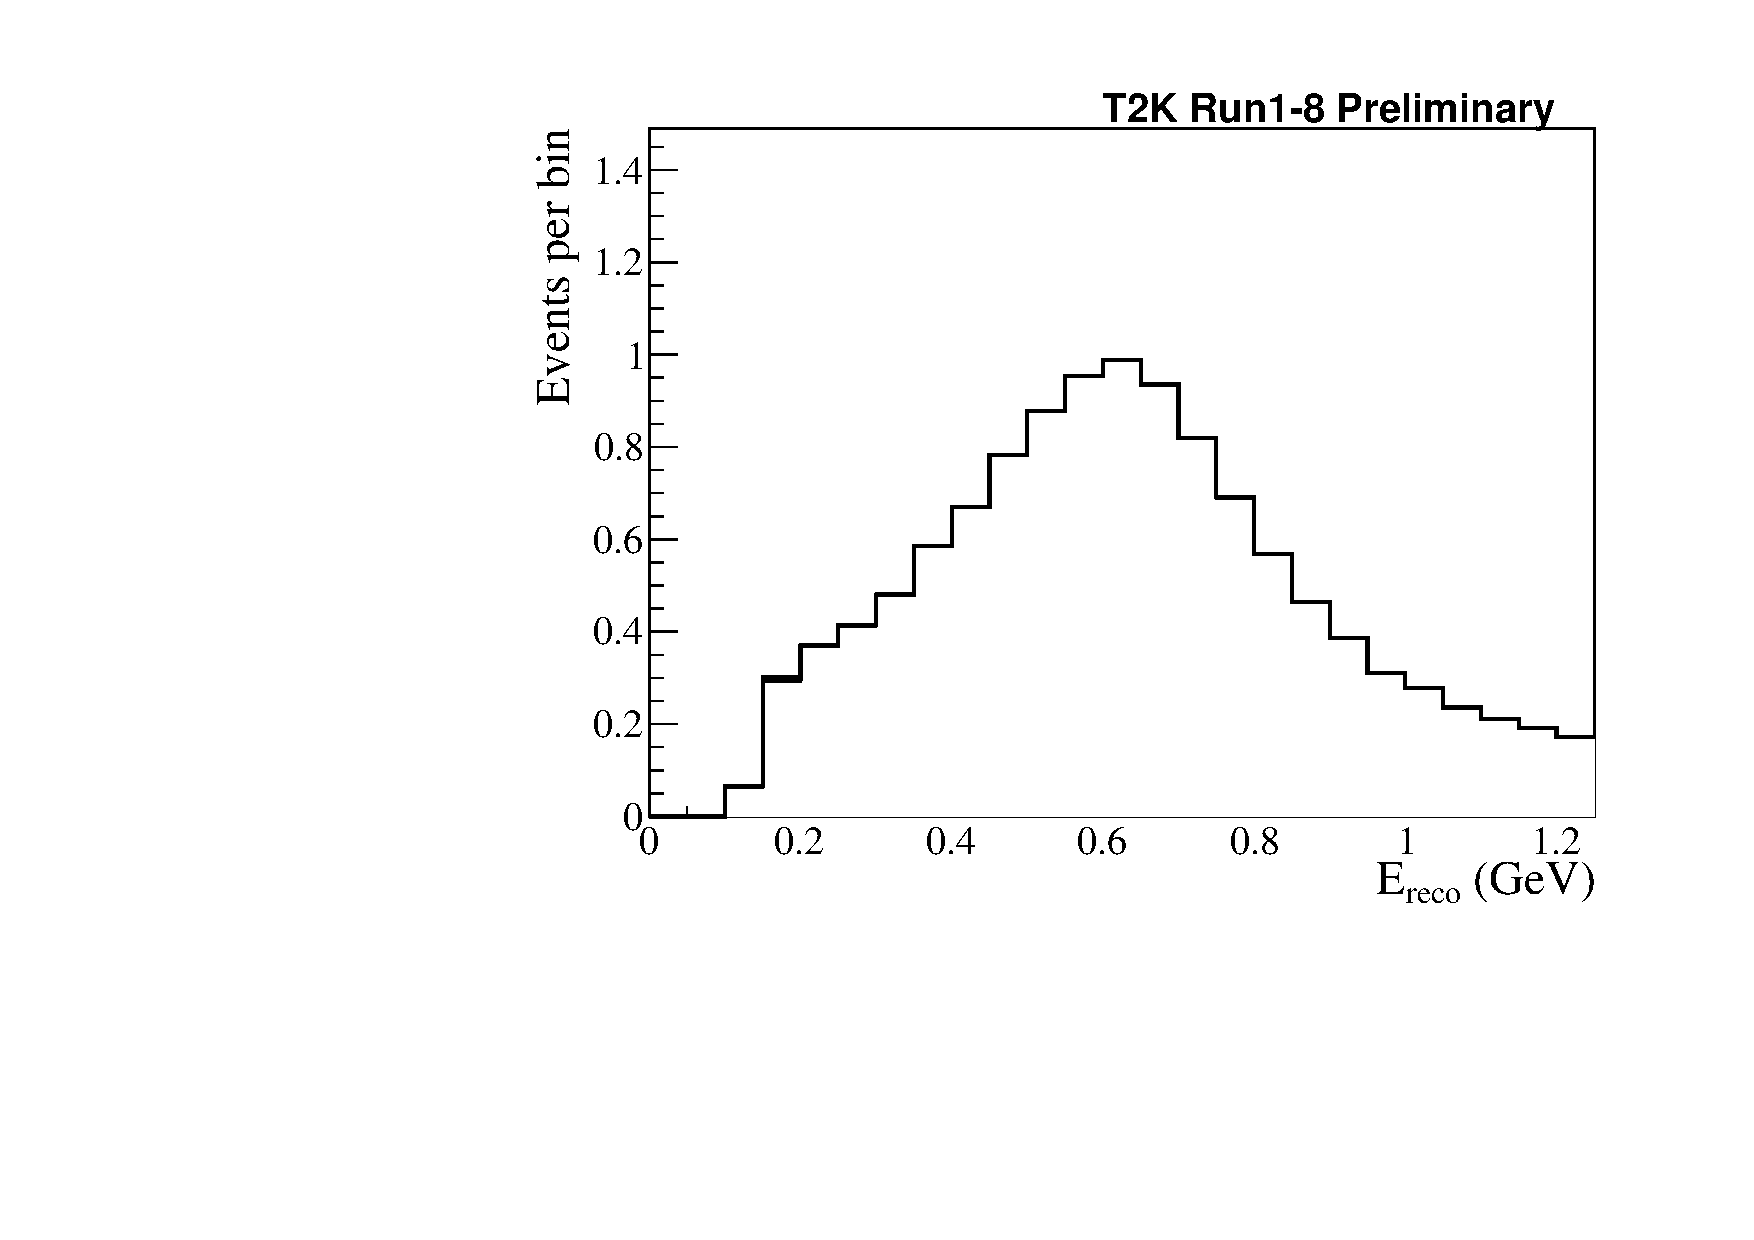
\includegraphics[width=0.9\textwidth]{images/systematics/envelopes/sk_error_table_RHC1Re_xsec_ncoth_envelope}
		\caption{Electron-like antineutrino mode}
	\end{subfigure}
	\begin{subfigure}[b]{0.49\textwidth}
		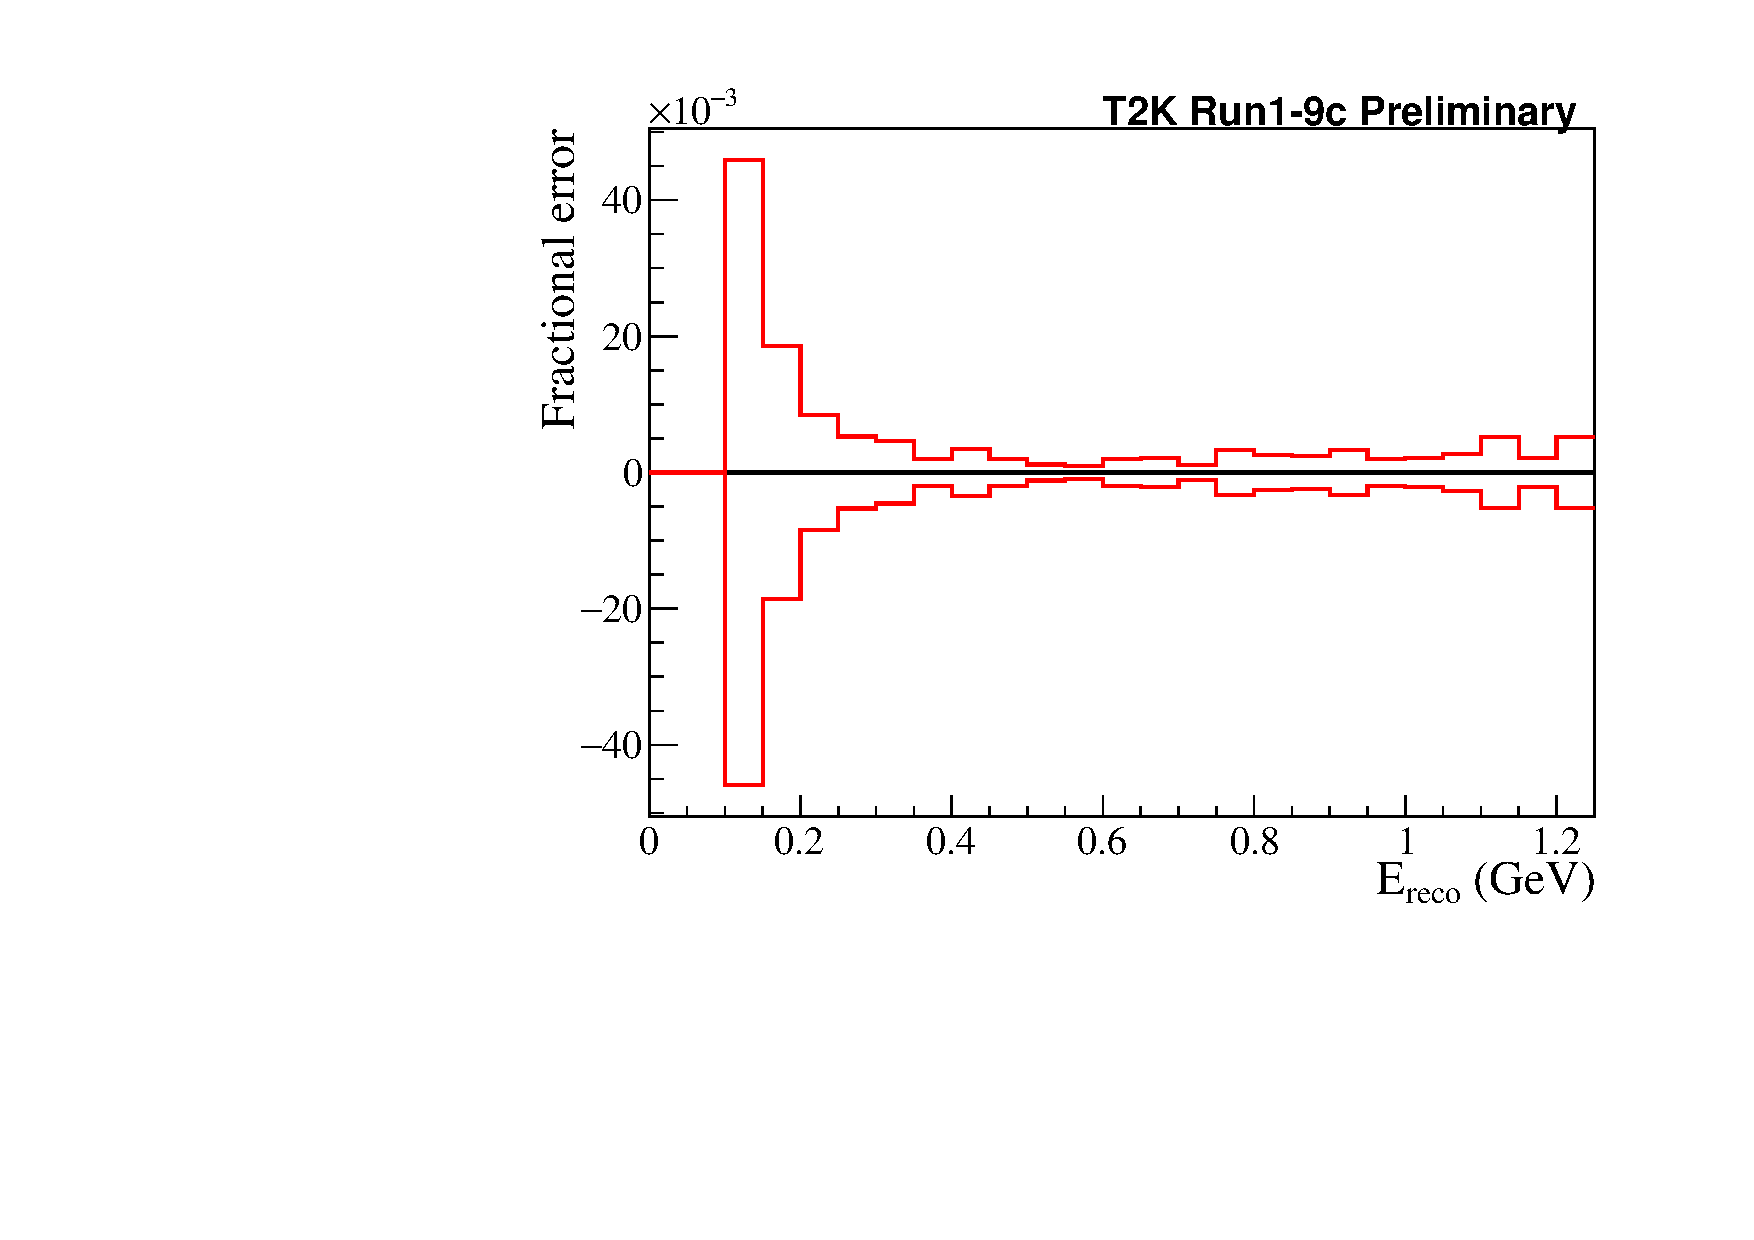
\includegraphics[width=0.9\textwidth]{images/systematics/envelopes/sk_error_table_RHC1Re_xsec_ncoth_envelope_fractional}
		\caption{Electron-like antineutrino mode}
	\end{subfigure}
	\caption {
		Error envelopes (left) and fractional errors (right) for the reconstructed neutrino energy spectrum for the unconstrained NCother systematic parameters. \NumToysSmall toys are generated for the Asimov data set A with randomized systematic parameters with correlations taken into account.
	}
	\label{fig:sk_envelopes_xsec_ncoth_b}
\end{figure*}
\clearpage
\begin{figure*}
	\center
	\begin{subfigure}[b]{0.49\textwidth}
		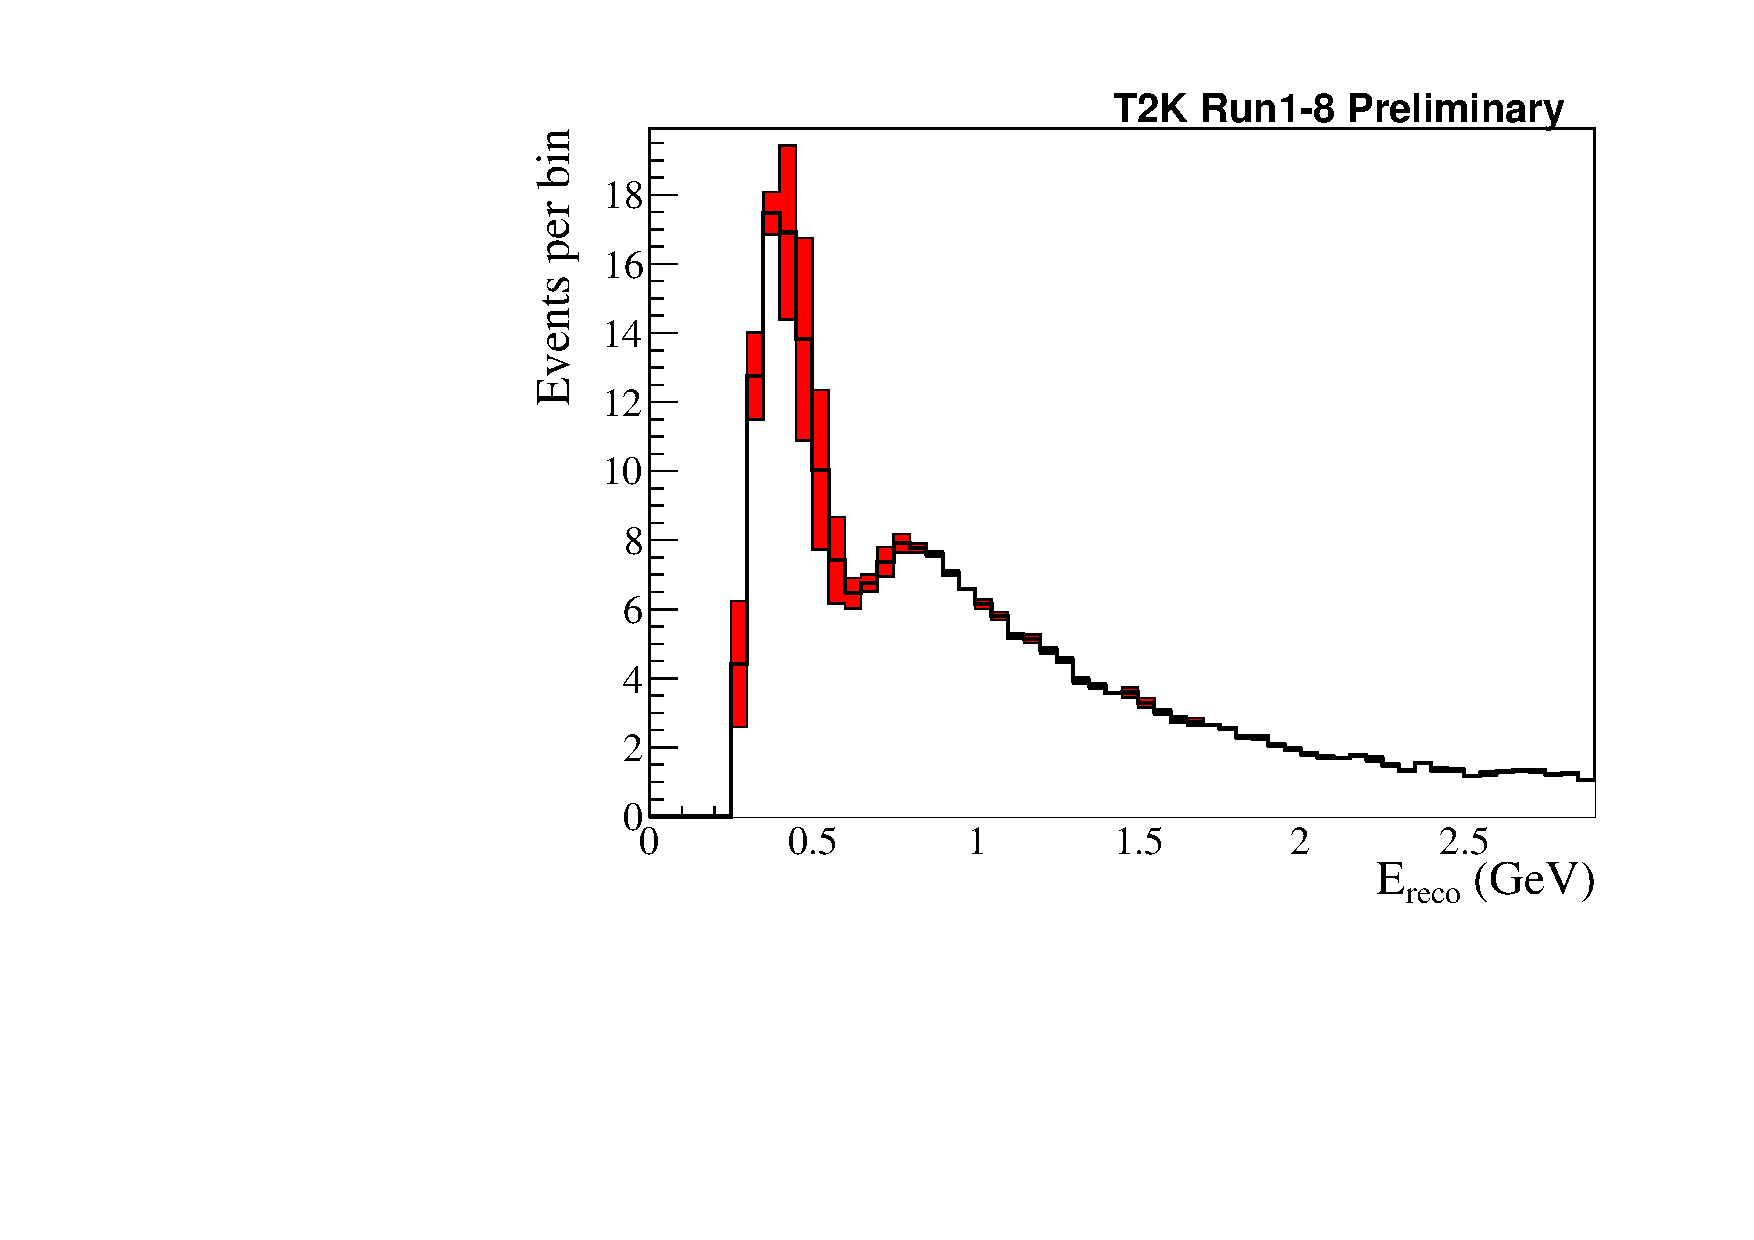
\includegraphics[width=0.9\textwidth]{images/systematics/envelopes/sk_error_table_1Rmu_xsec_eb_envelope}
		\caption{Muon-like, neutrino mode}
	\end{subfigure}
	\begin{subfigure}[b]{0.49\textwidth}
		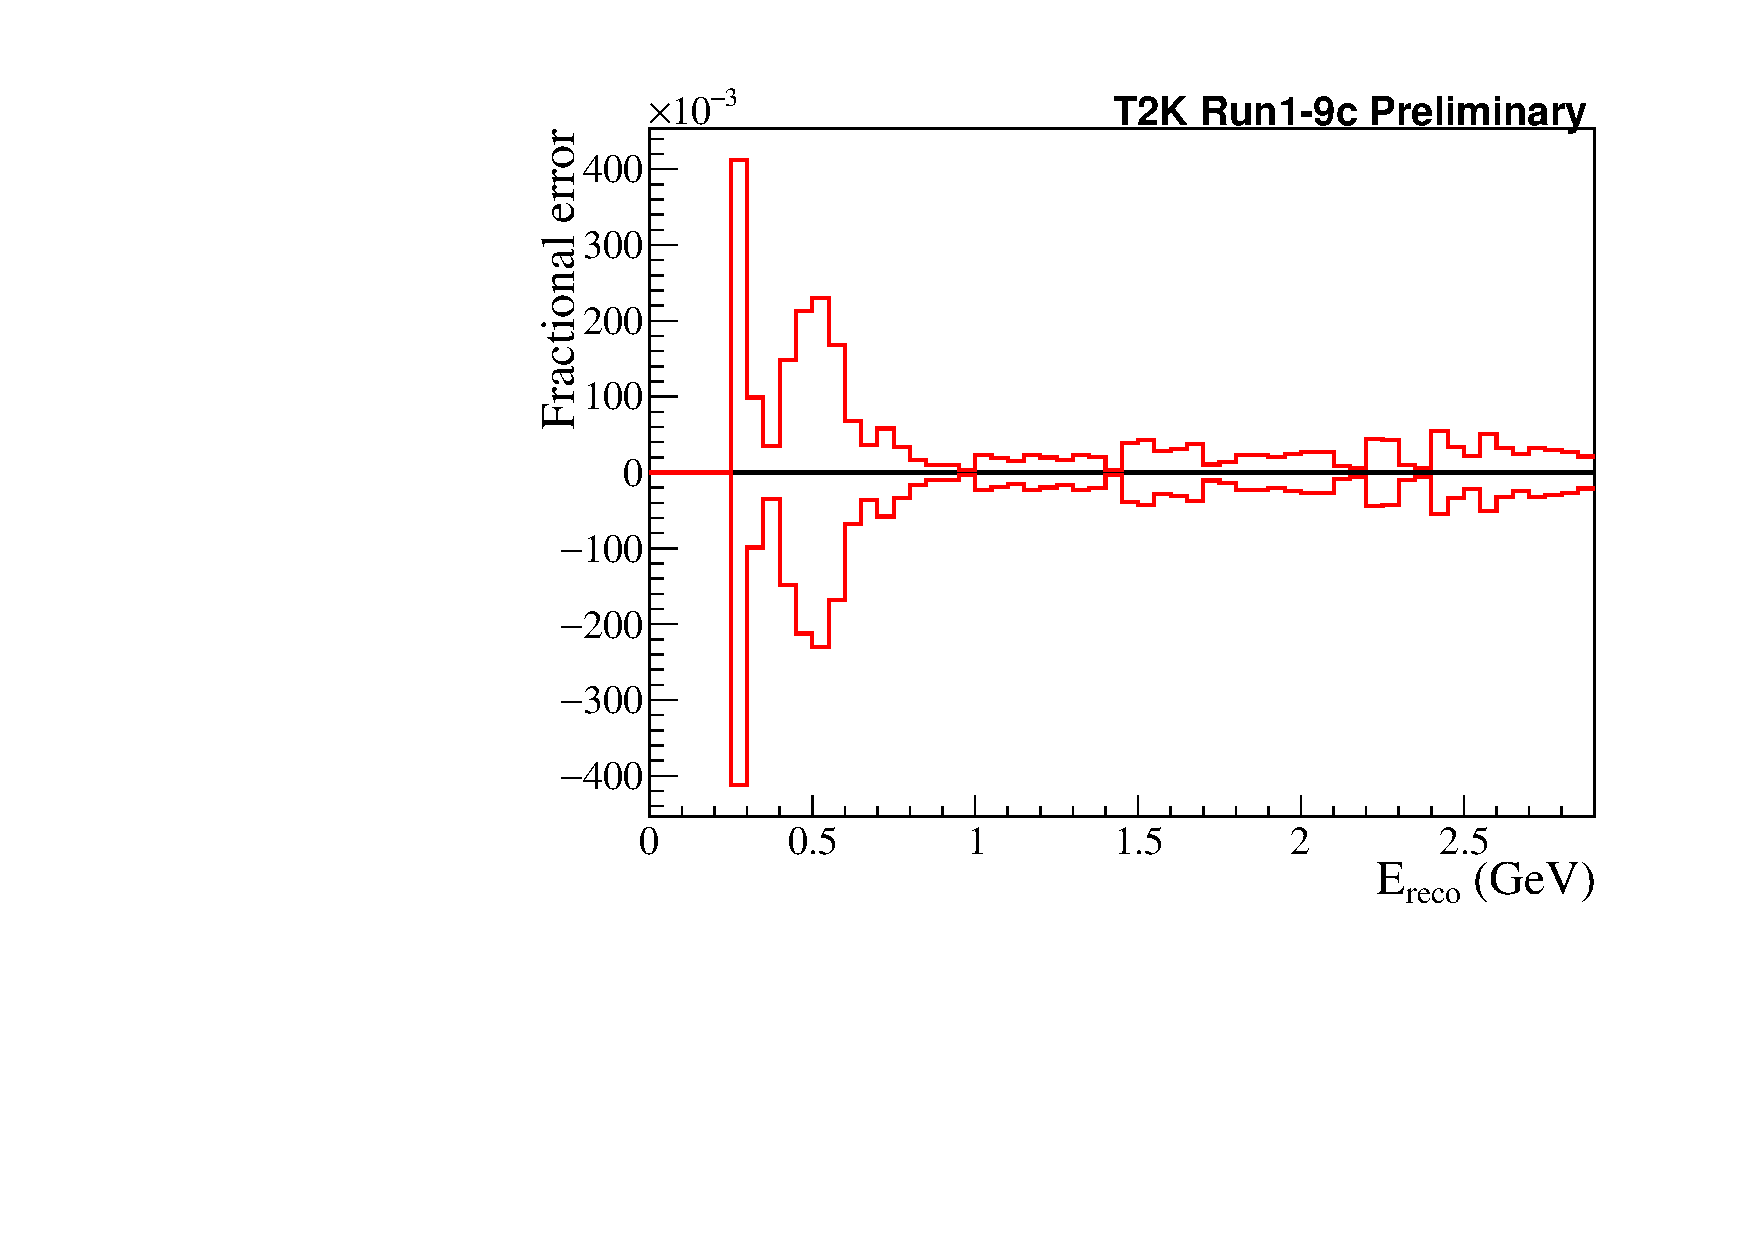
\includegraphics[width=0.9\textwidth]{images/systematics/envelopes/sk_error_table_1Rmu_xsec_eb_envelope_fractional}
		\caption{Muon-like, neutrino mode}
	\end{subfigure}
	\begin{subfigure}[b]{0.49\textwidth}
		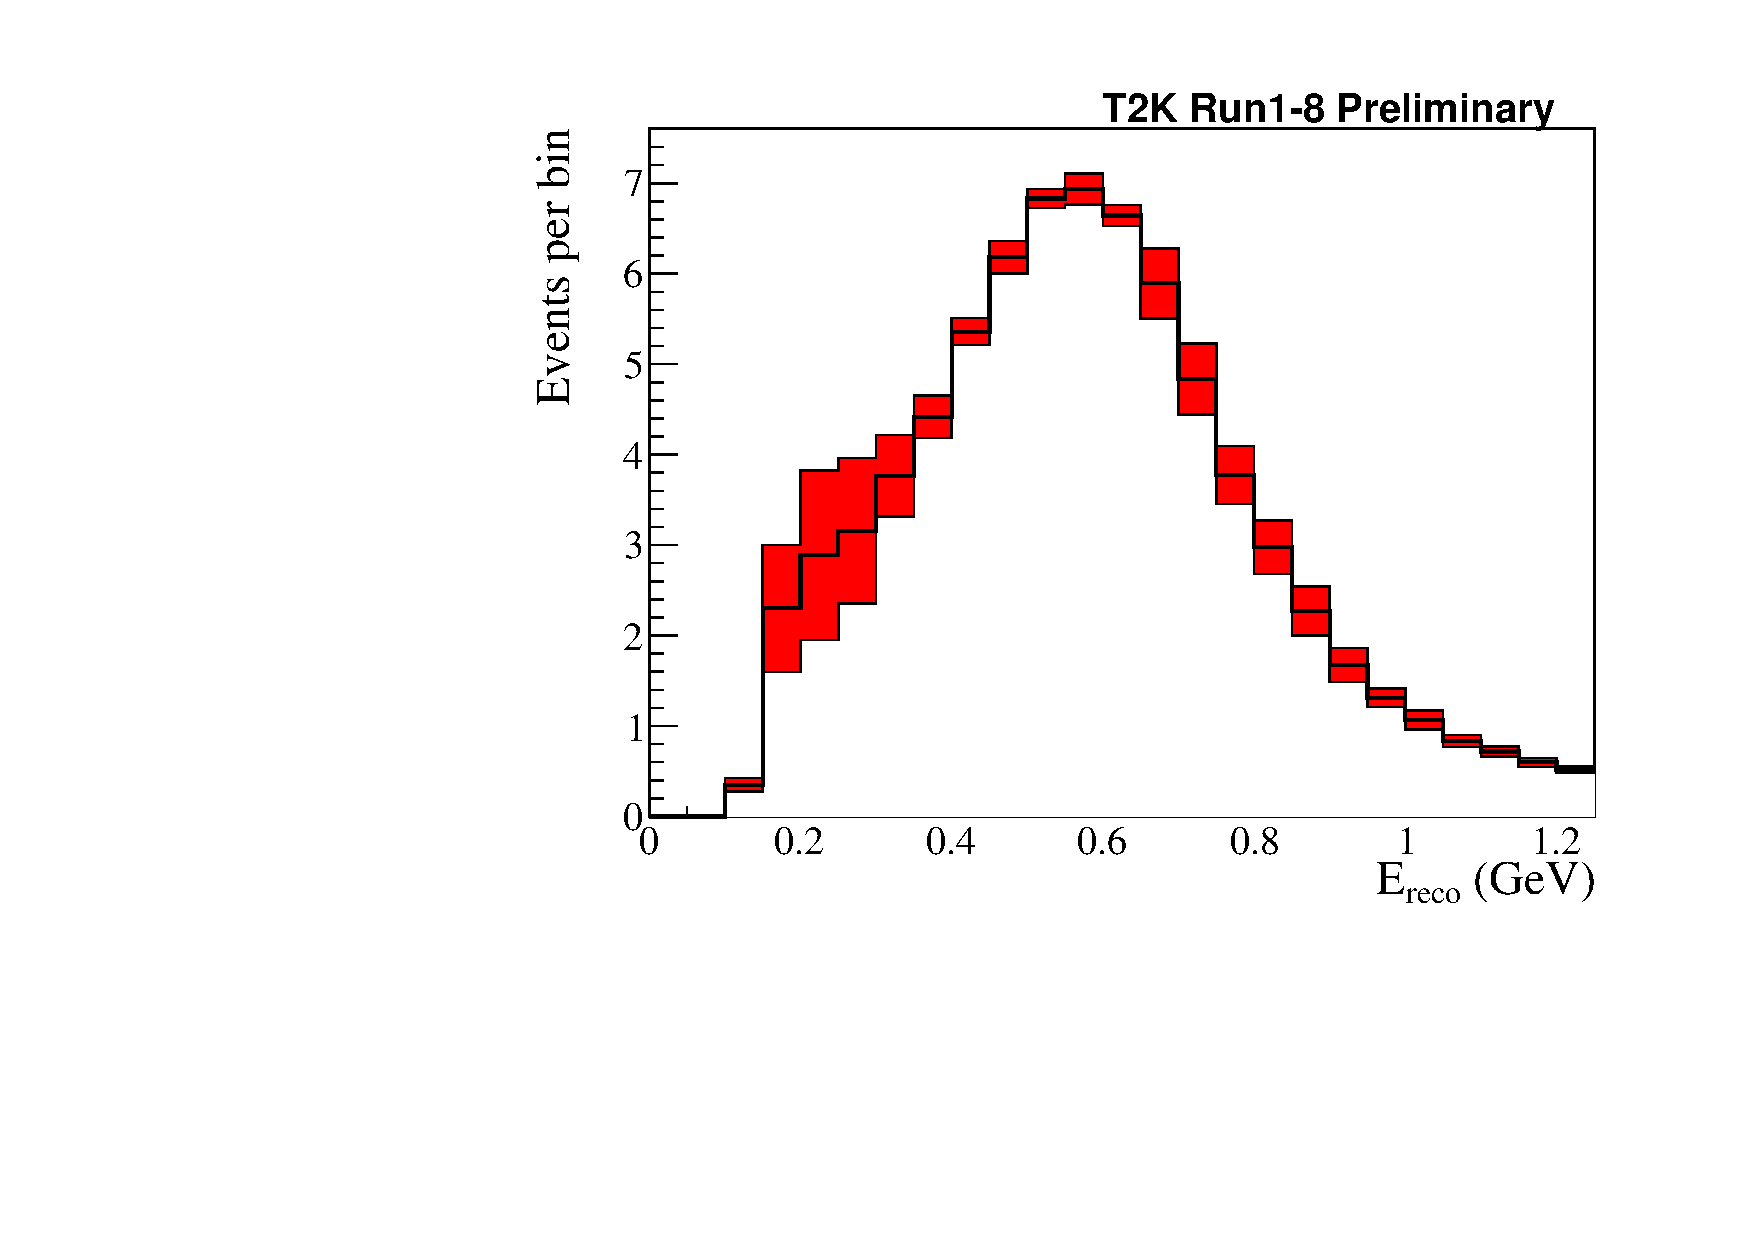
\includegraphics[width=0.9\textwidth]{images/systematics/envelopes/sk_error_table_1Re_xsec_eb_envelope}
		\caption{Electron-like, neutrino mode}
	\end{subfigure}
	\begin{subfigure}[b]{0.49\textwidth}
		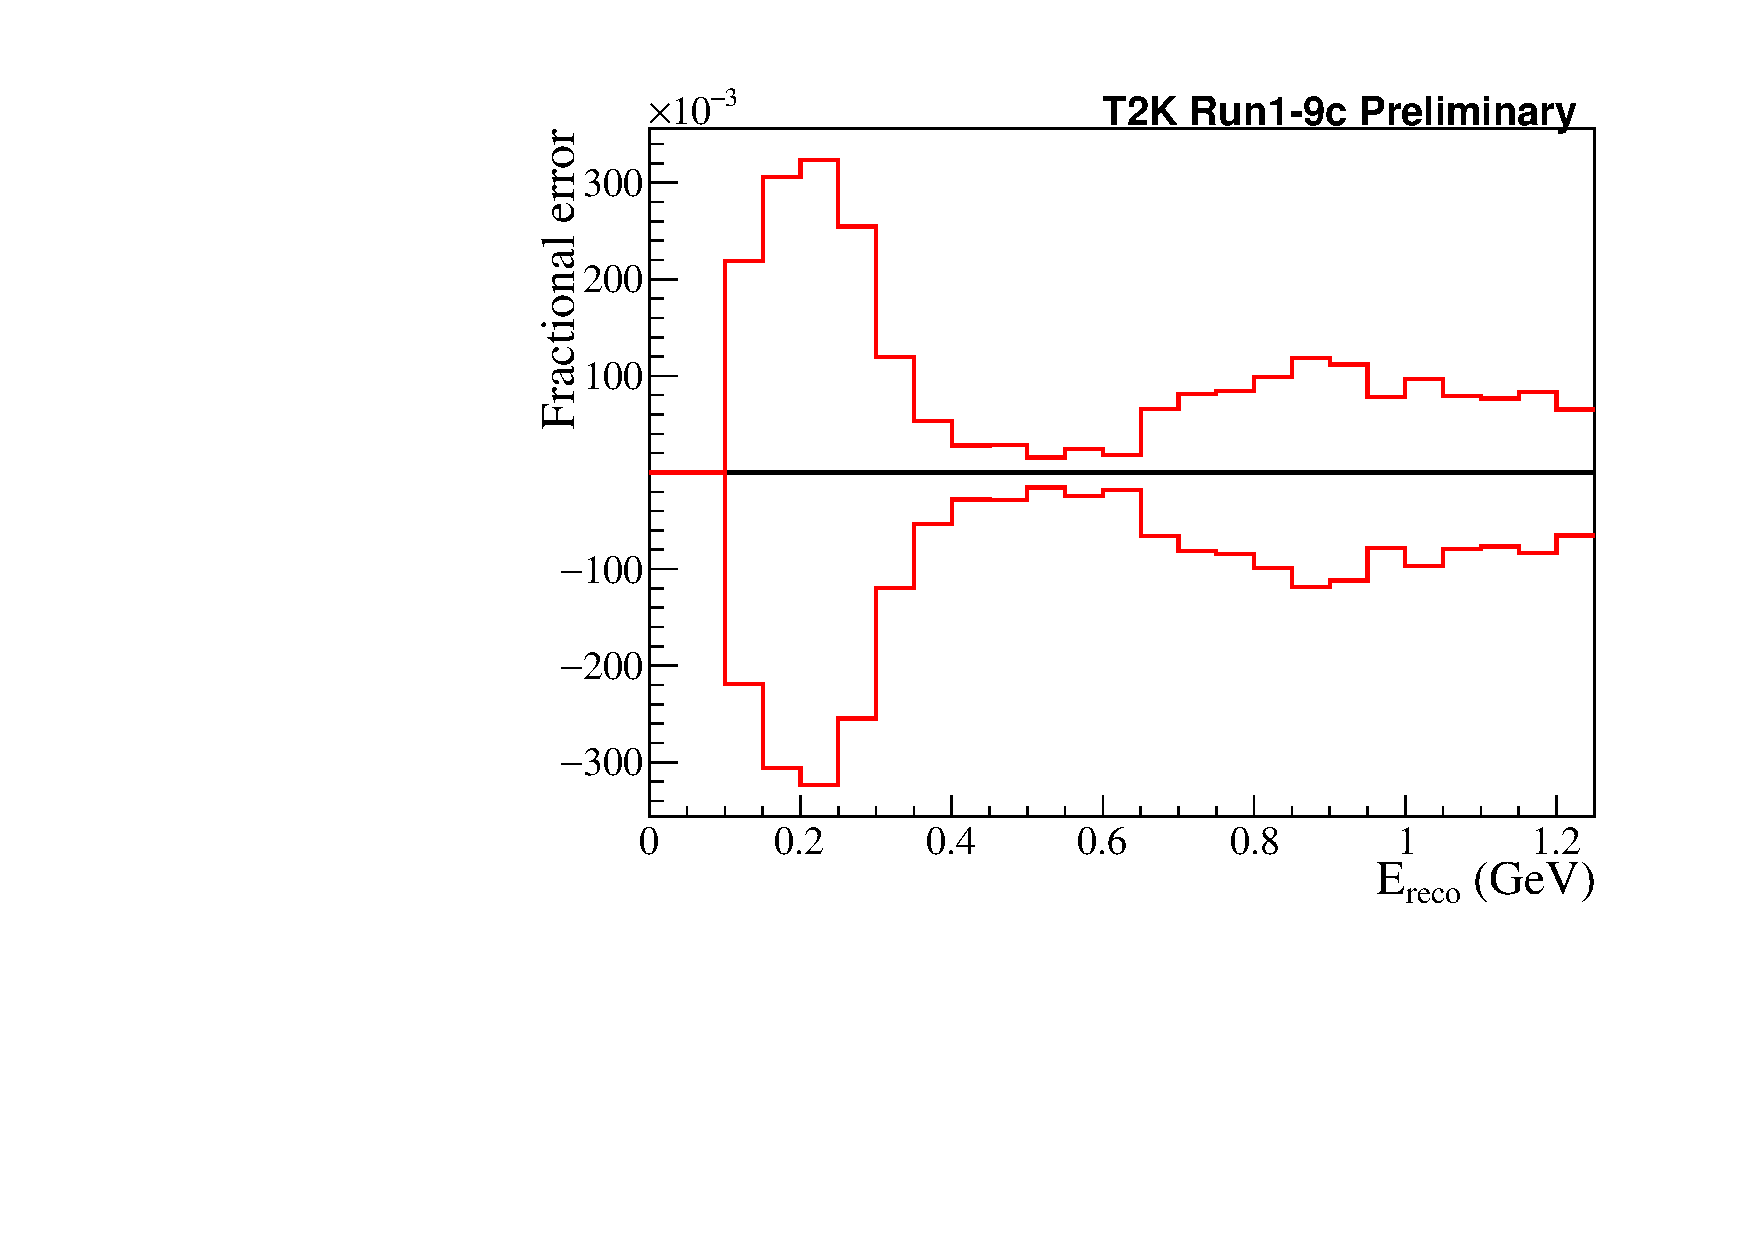
\includegraphics[width=0.9\textwidth]{images/systematics/envelopes/sk_error_table_1Re_xsec_eb_envelope_fractional}
		\caption{Electron-like, neutrino mode}
	\end{subfigure}
	\begin{subfigure}[b]{0.49\textwidth}
		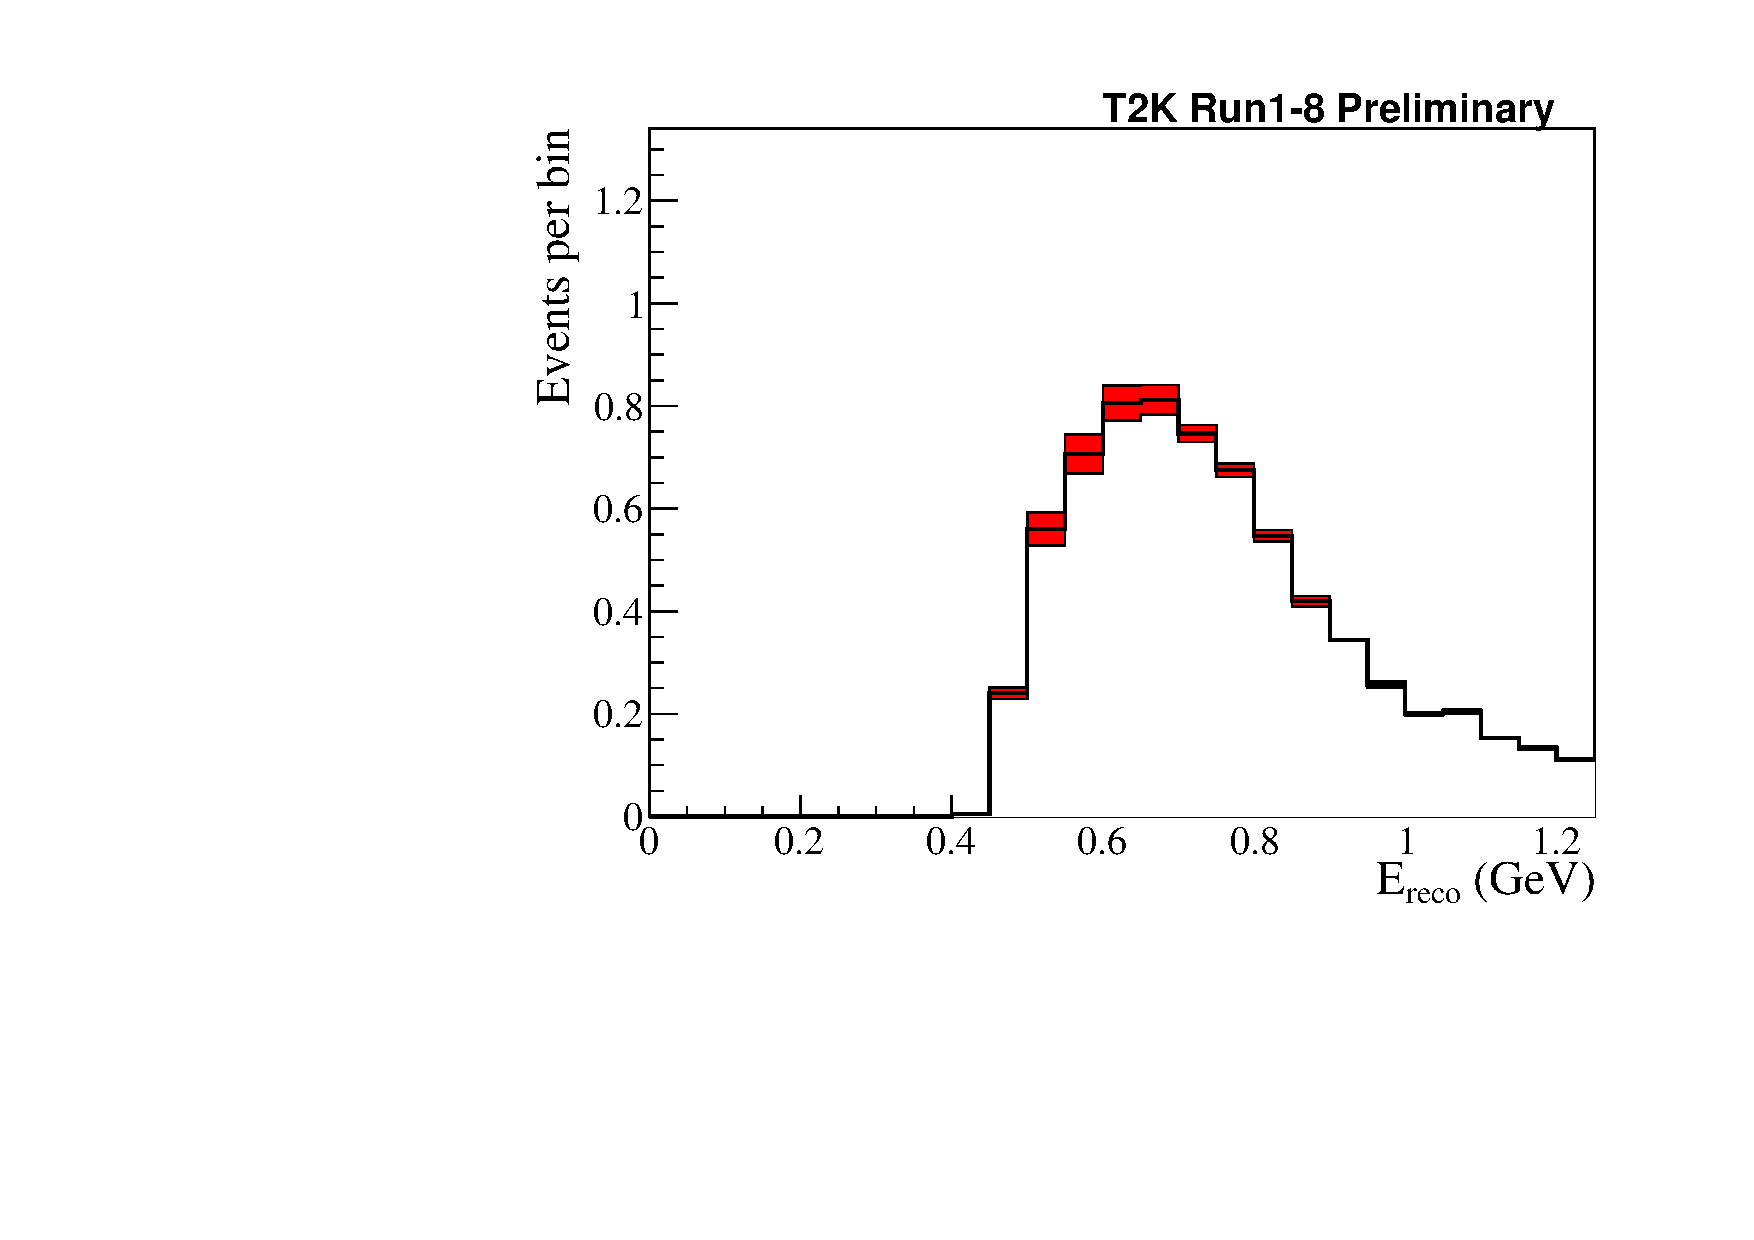
\includegraphics[width=0.9\textwidth]{images/systematics/envelopes/sk_error_table_MultiRe_xsec_eb_envelope}
		\caption{\nueCConepi-like, neutrino mode}
	\end{subfigure}
	\begin{subfigure}[b]{0.49\textwidth}
		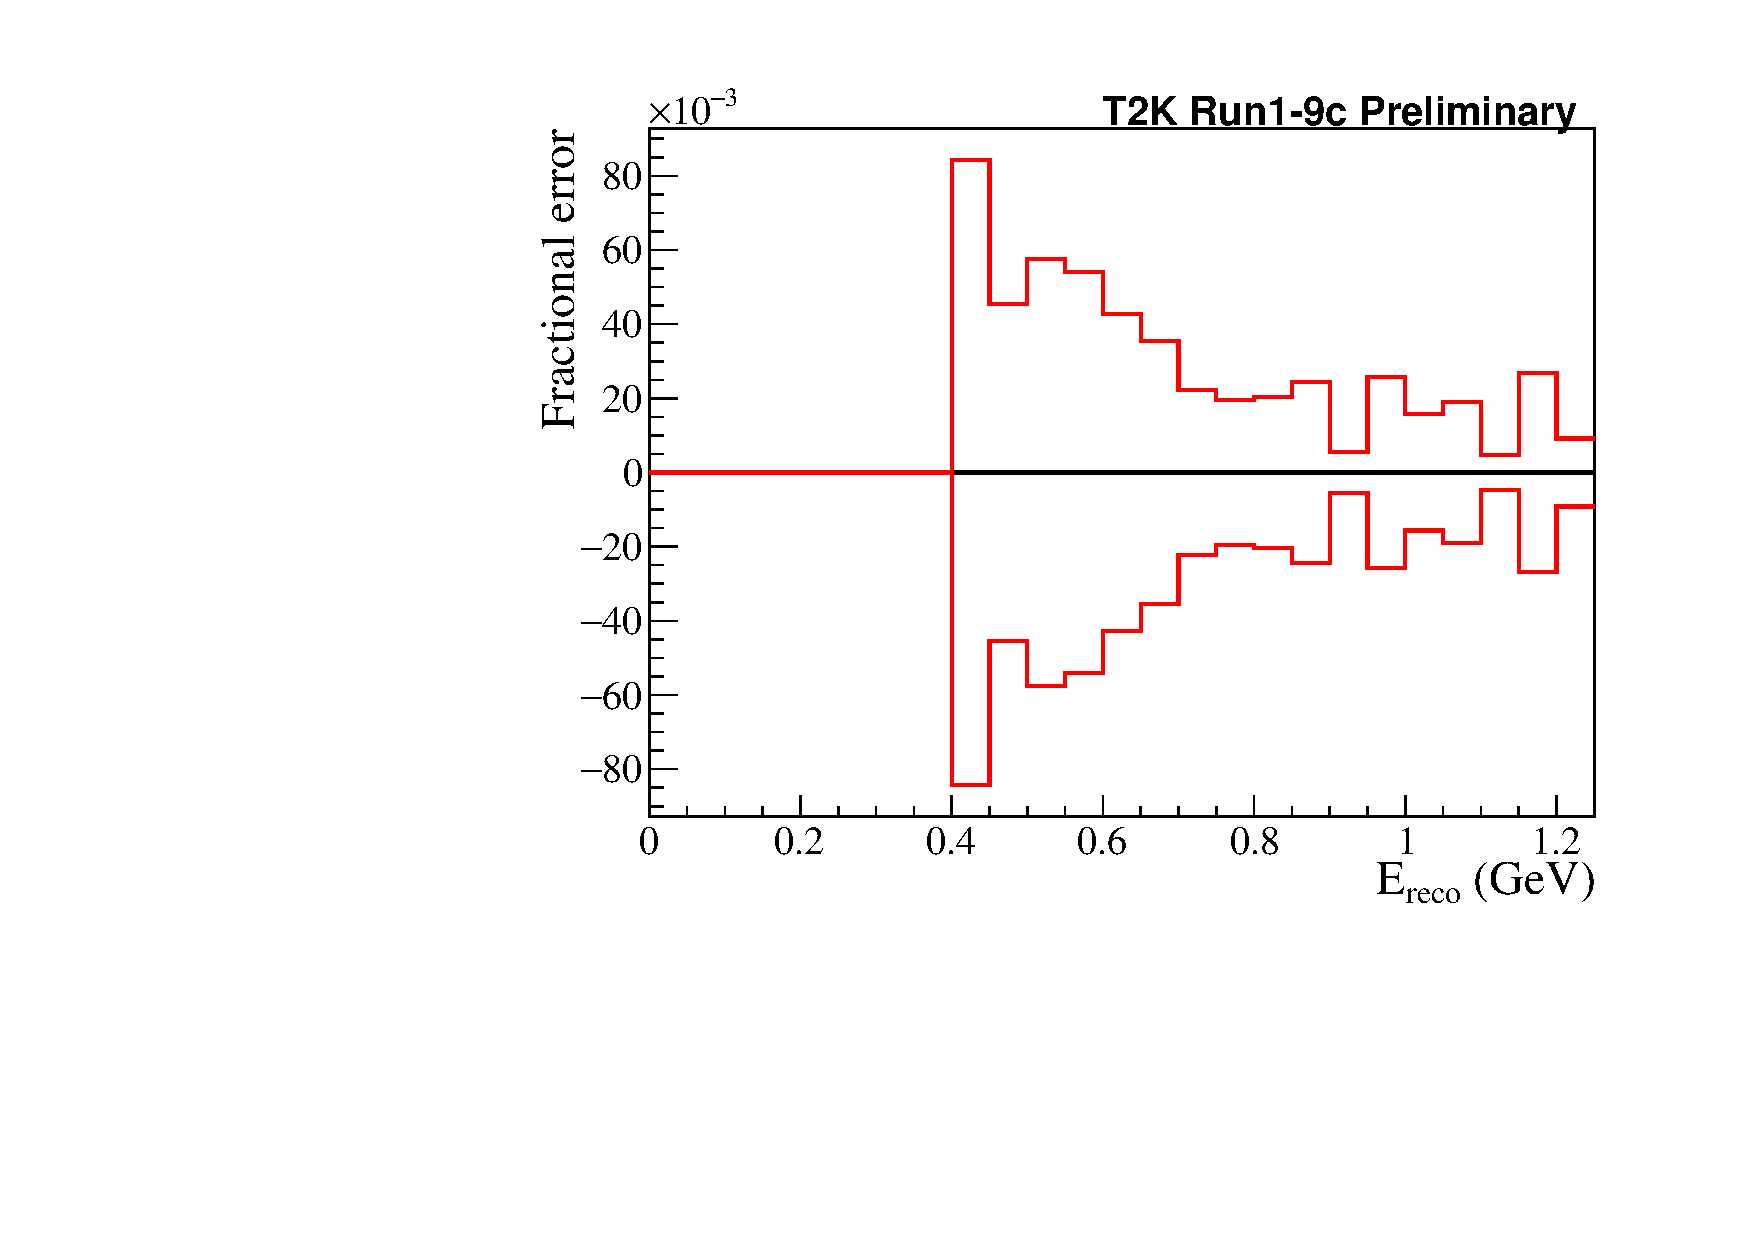
\includegraphics[width=0.9\textwidth]{images/systematics/envelopes/sk_error_table_MultiRe_xsec_eb_envelope_fractional}
		\caption{\nueCConepi-like, neutrino mode}
	\end{subfigure}
	\caption {
		Error envelopes (left) and fractional errors (right) for the reconstructed neutrino energy spectrum for the unconstrained $E_b$ systematic parameter. \NumToysSmall toys are generated for the Asimov data set A with randomized systematic parameters with correlations taken into account.
	}
	\label{fig:sk_envelopes_xsec_eb}
\end{figure*}
\clearpage

\begin{figure*}
	\center
	\begin{subfigure}[b]{0.49\textwidth}
		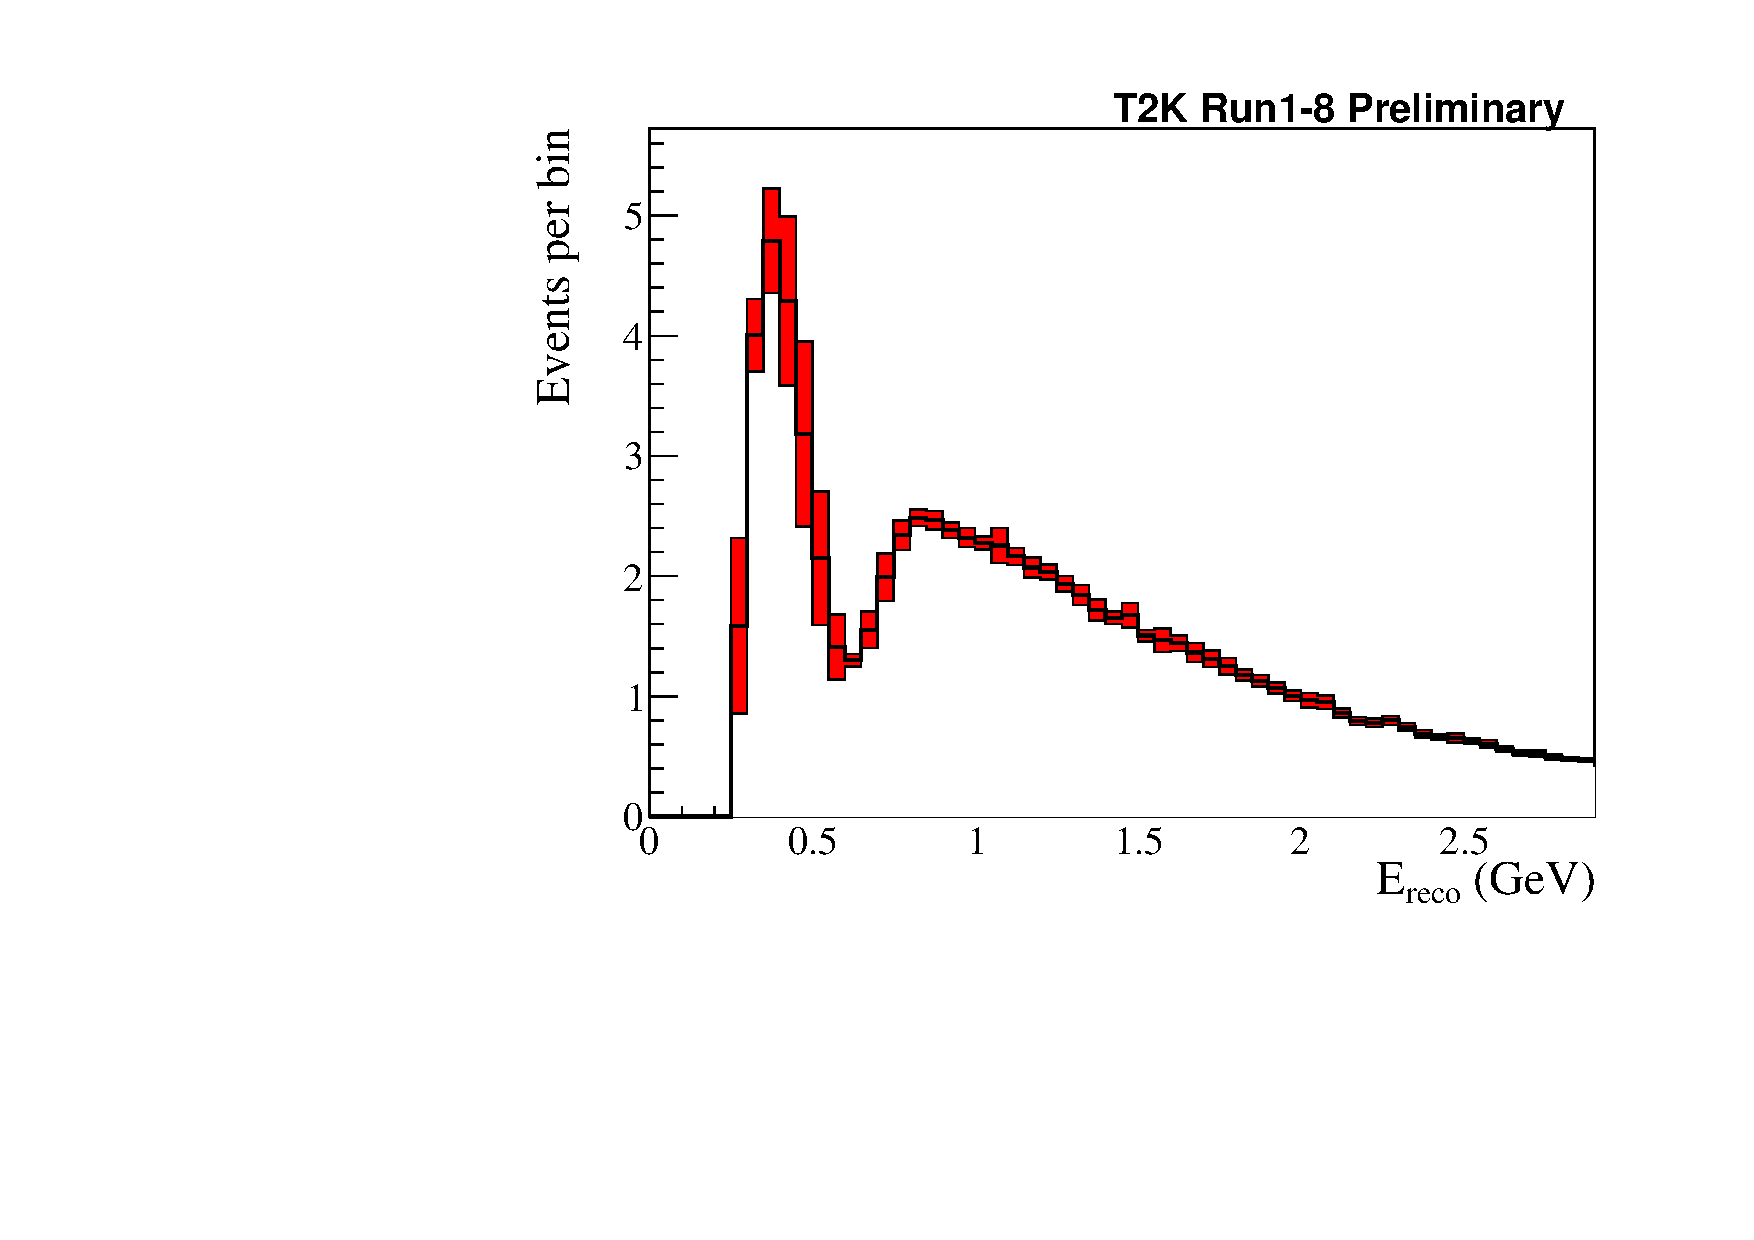
\includegraphics[width=0.9\textwidth]{images/systematics/envelopes/sk_error_table_RHC1Rmu_xsec_eb_envelope}
		\caption{Muon-like, antineutrino mode}
	\end{subfigure}
	\begin{subfigure}[b]{0.49\textwidth}
		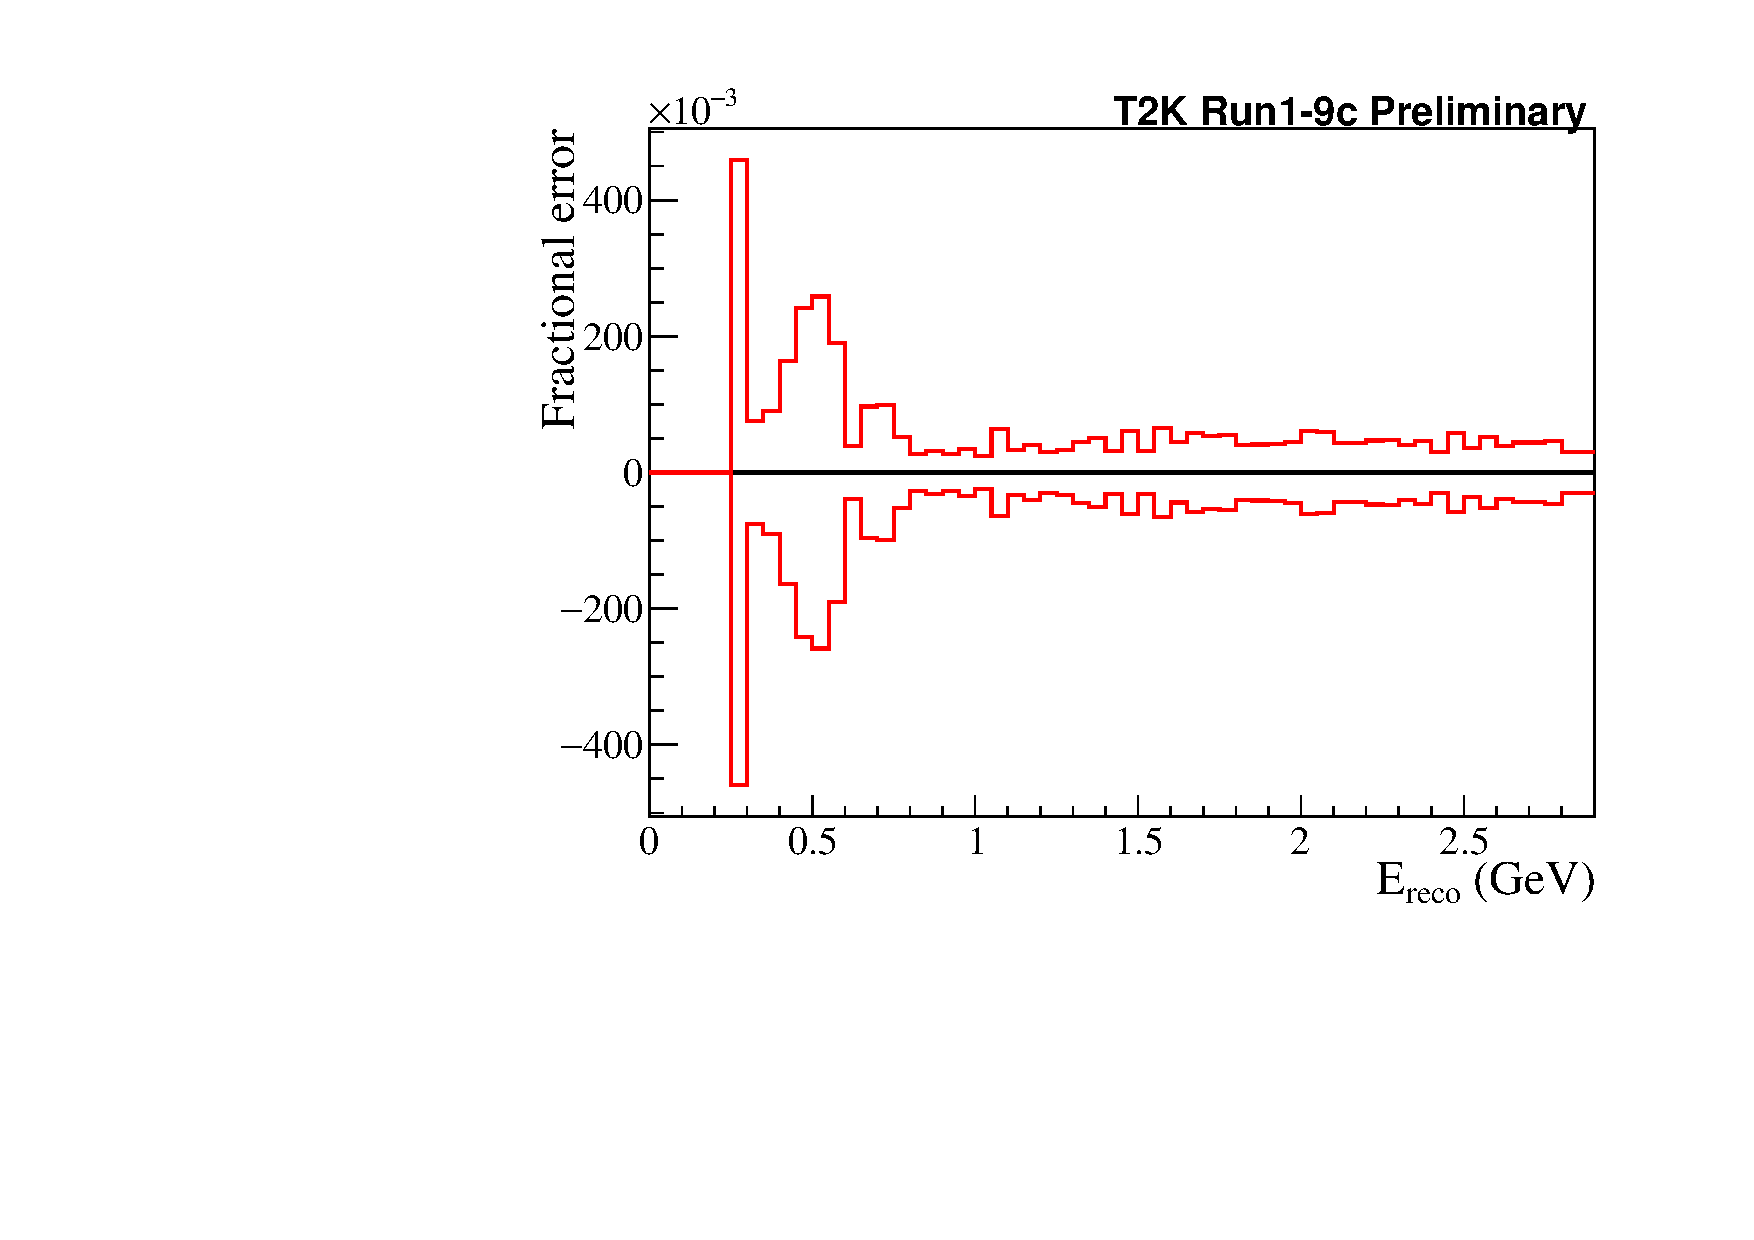
\includegraphics[width=0.9\textwidth]{images/systematics/envelopes/sk_error_table_RHC1Rmu_xsec_eb_envelope_fractional}
		\caption{Muon-like, antineutrino mode}
	\end{subfigure}
	\begin{subfigure}[b]{0.49\textwidth}
		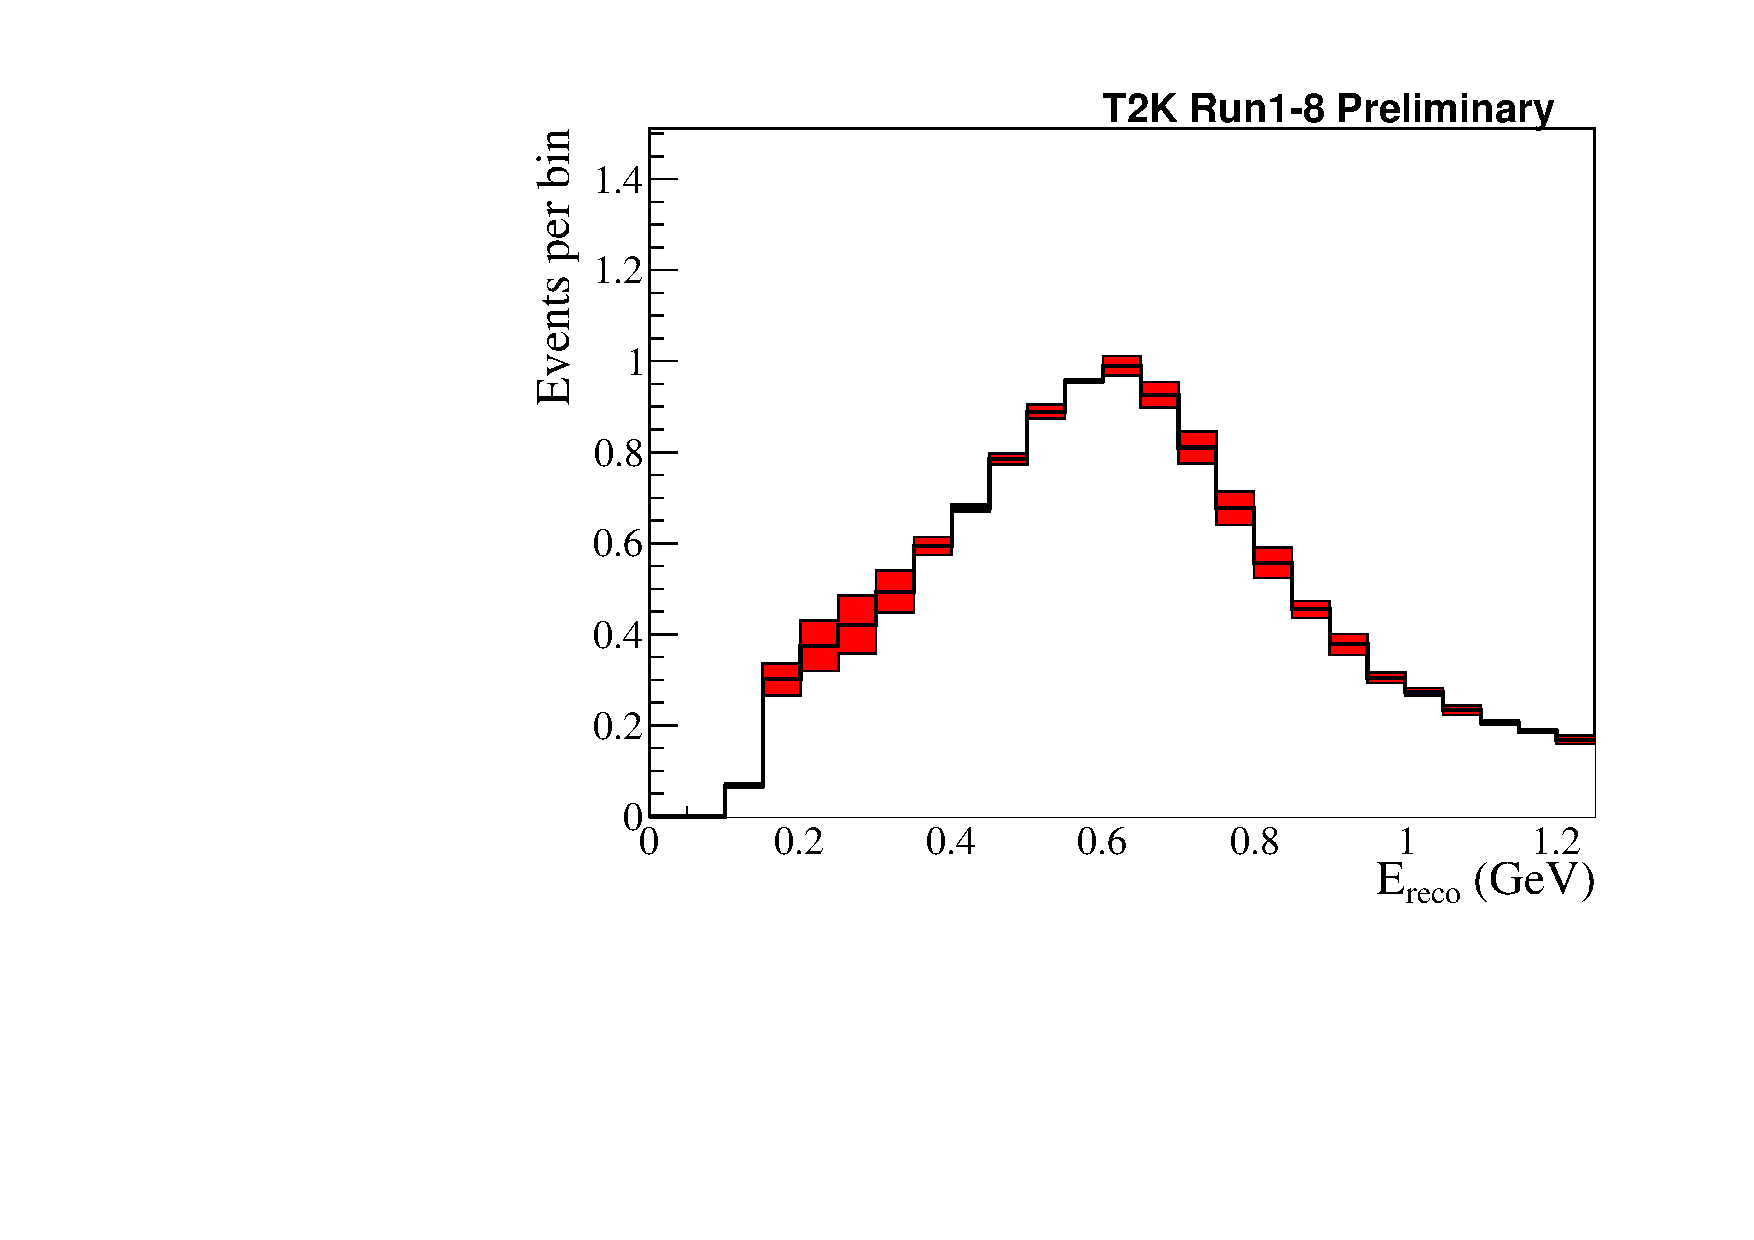
\includegraphics[width=0.9\textwidth]{images/systematics/envelopes/sk_error_table_RHC1Re_xsec_eb_envelope}
		\caption{Electron-like antineutrino mode}
	\end{subfigure}
	\begin{subfigure}[b]{0.49\textwidth}
		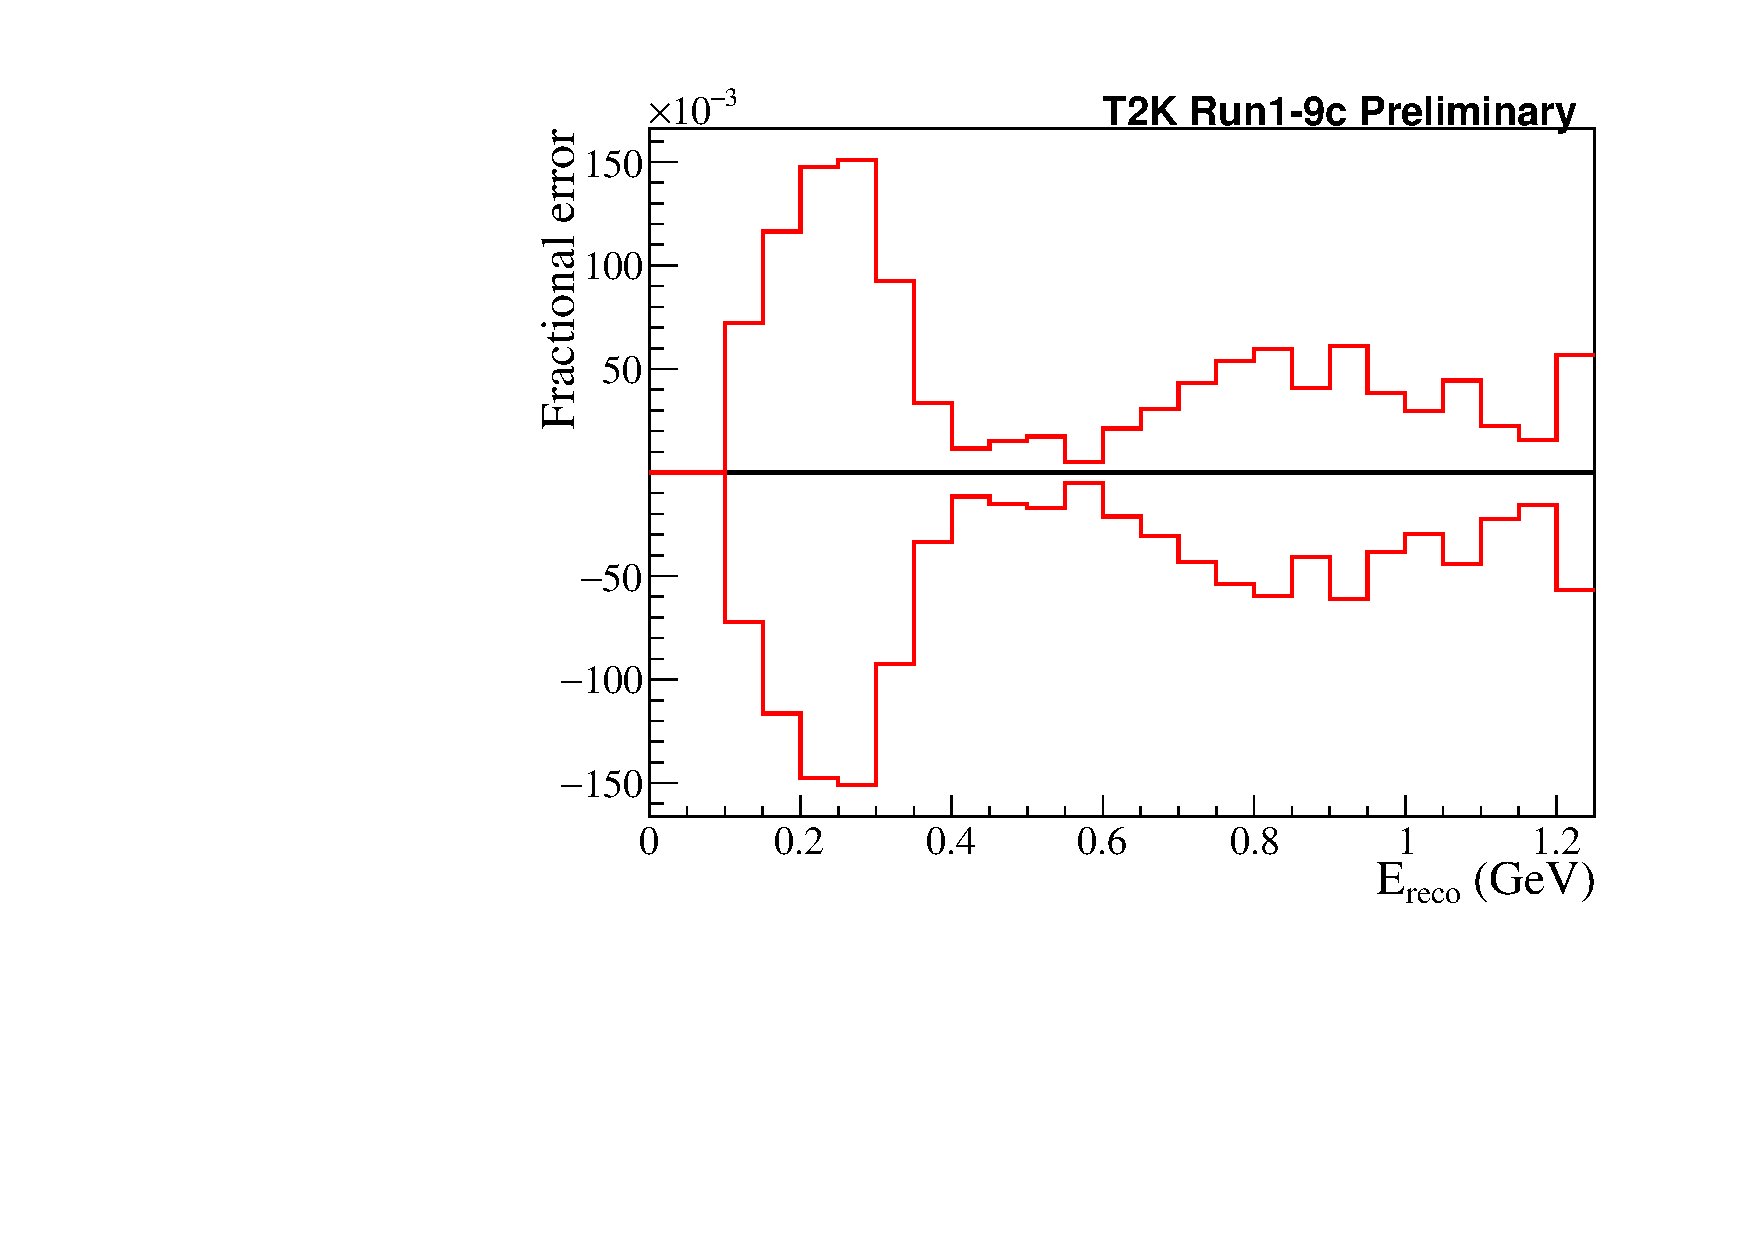
\includegraphics[width=0.9\textwidth]{images/systematics/envelopes/sk_error_table_RHC1Re_xsec_eb_envelope_fractional}
		\caption{Electron-like antineutrino mode}
	\end{subfigure}
	\caption {
		Error envelopes (left) and fractional errors (right) for the reconstructed neutrino energy spectrum for the unconstrained $E_b$ systematic parameter. \NumToysSmall toys are generated for the Asimov data set A with randomized systematic parameters with correlations taken into account.
	}
	\label{fig:sk_envelopes_xsec_eb_b}
\end{figure*}
\clearpage
\FloatBarrier
\clearpage
	\section{Asimov B \deltacp/mass-hierarchy degeneracy}
\label{app:asimovb_sensitivity}

In \cref{sec:sensitivity:asimov_results} it was noted that Asimov B fits are affected by a lack of sensitivity to distinguish $\delta_{CP} = 0$ and $\delta_{CP} = \pi$, for example, the fit of \deltacp shown in \cref{fig:ssqth13_vs_dcp_sensitivity} shows a best-fit point shifted away from the true value. \cref{fig:asimovb_spectra_degeneracy} shows normalised one-ring $e$-like spectra for Asimov data set B with mass hierarchy and \deltacp varied to demonstrate the problem. It is clear from the plots that the spectrum for $\delta_{CP} = 0$ in normal hierarchy is similar in shape to the spectrum for $\delta_{CP} = \pi$ in inverted hierarchy and vice versa.

\begin{figure*}[htb]
	\begin{subfigure}[b]{0.49\textwidth}
		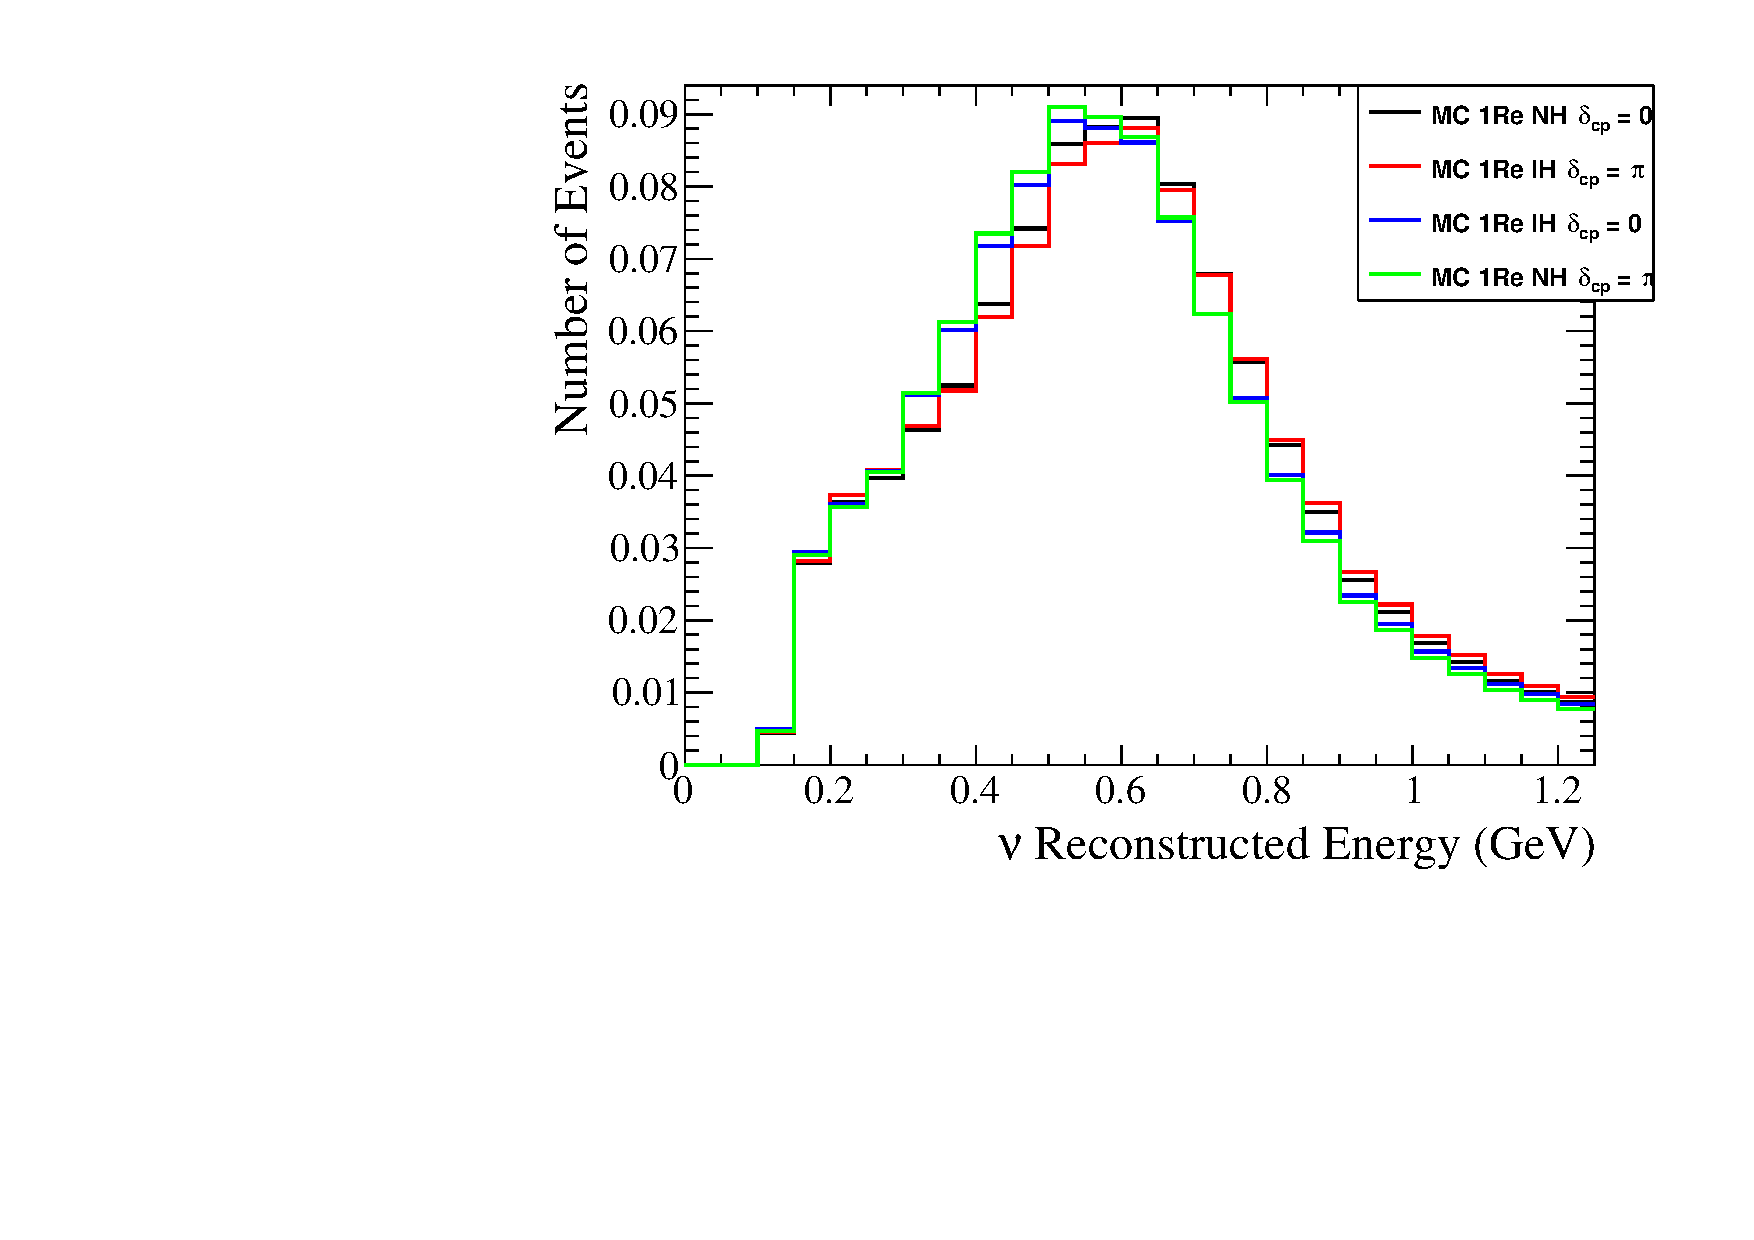
\includegraphics[width=0.9\textwidth]{images/spectra/asimovb_degeneracy_fhc}
		\caption{MC one-ring FHC $e$-like spectra}
	\end{subfigure}
	\begin{subfigure}[b]{0.49\textwidth}
		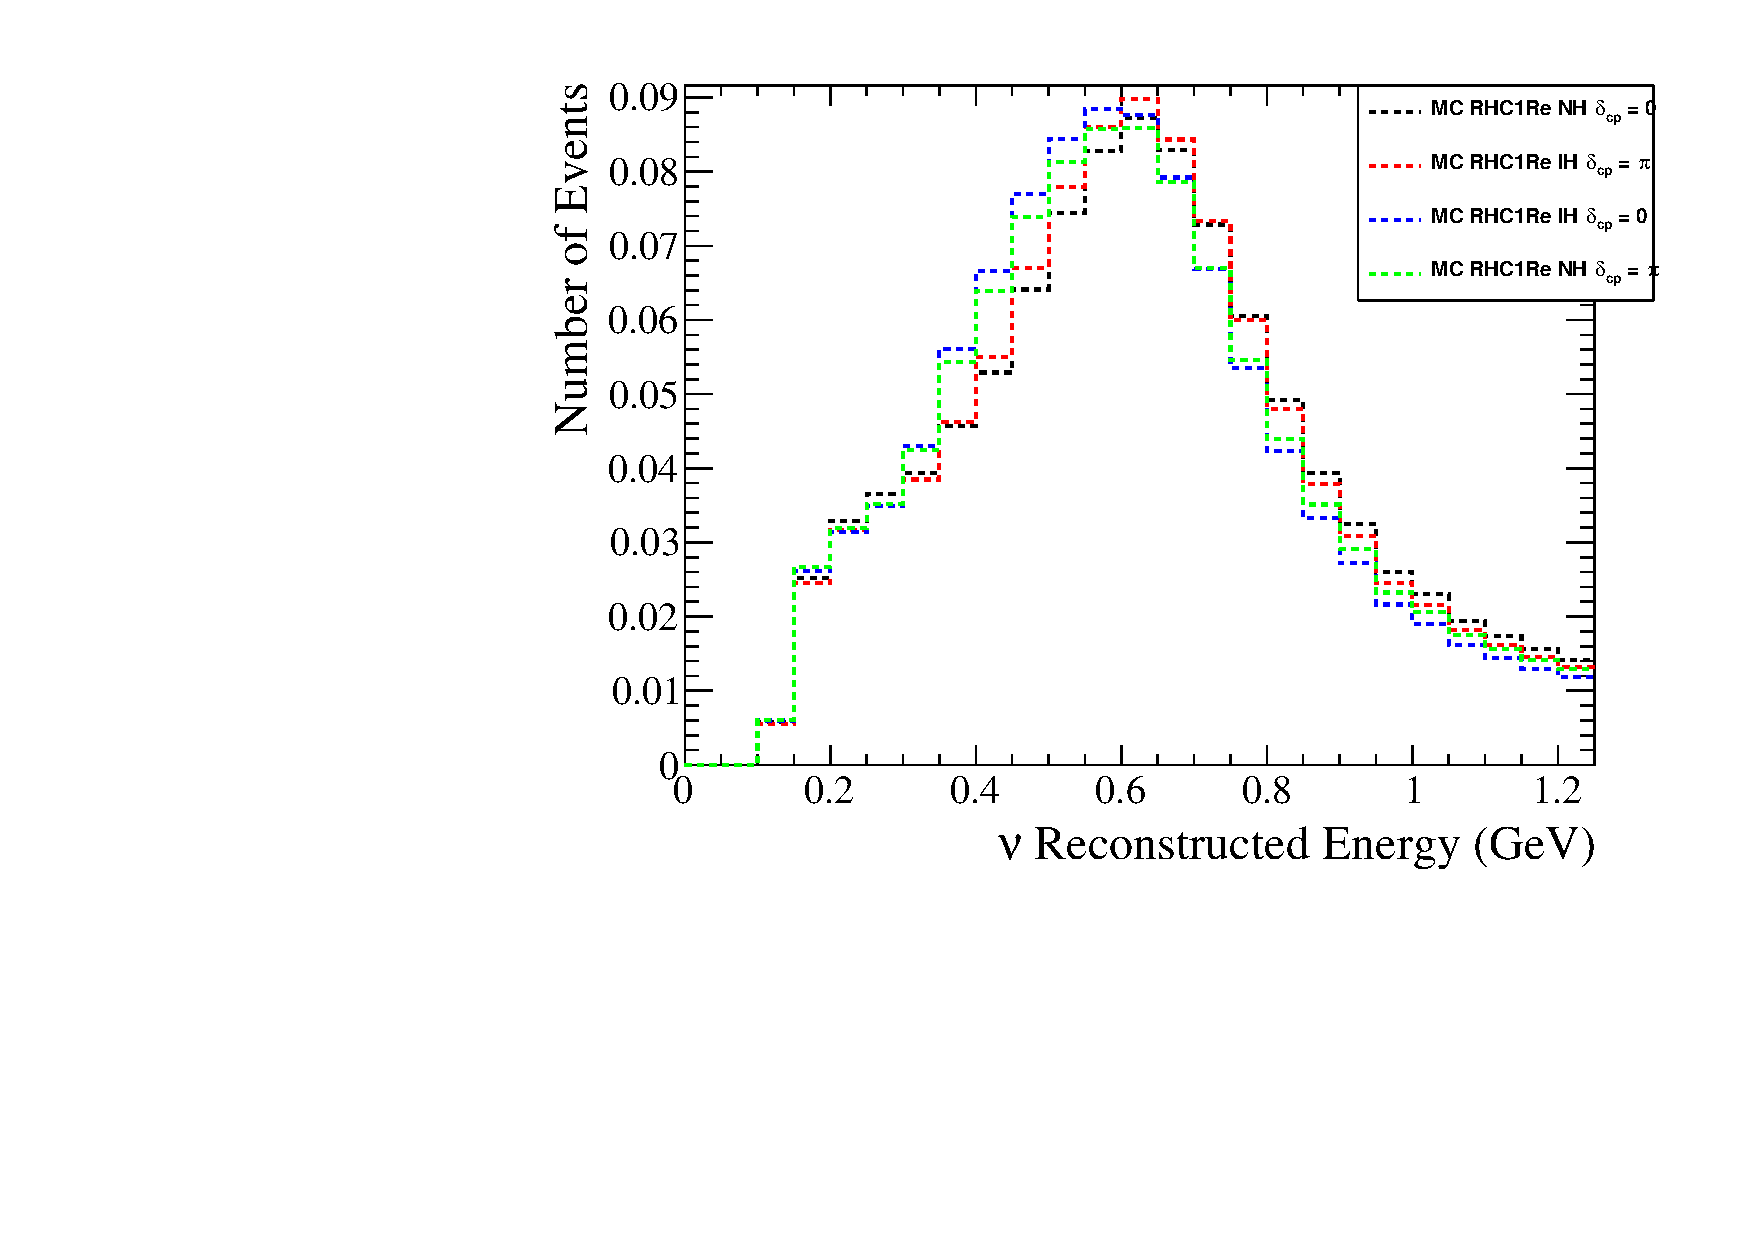
\includegraphics[width=0.9\textwidth]{images/spectra/asimovb_degeneracy_rhc}
		\caption{MC one-ring RHC $e$-like spectra}
	\end{subfigure}
	\caption {
		Normalised spectra for one-ring $e$-like samples showing the effect of changing the mass hierarchy and true value of \deltacp for the Asimov B data set.
	}
	\label{fig:asimovb_spectra_degeneracy}
\end{figure*}
\clearpage
	\clearpage

\section{Comparison of \RunPeriod data results to Asimov A sensitivities}
\label{app:data_asimov_comparison}

This chapter compares the results for the current \RunPeriod data set against the Asimov A sensitivities.

\subsection{Results for \appearance}
In \cref{fig:ssqth13_vs_dcp_data_asimov_compare} the result for \appearance with reactor constraint and T2K only is shown.

\begin{figure*}[htb]
	\center
	\begin{subfigure}[b]{0.49\textwidth}
		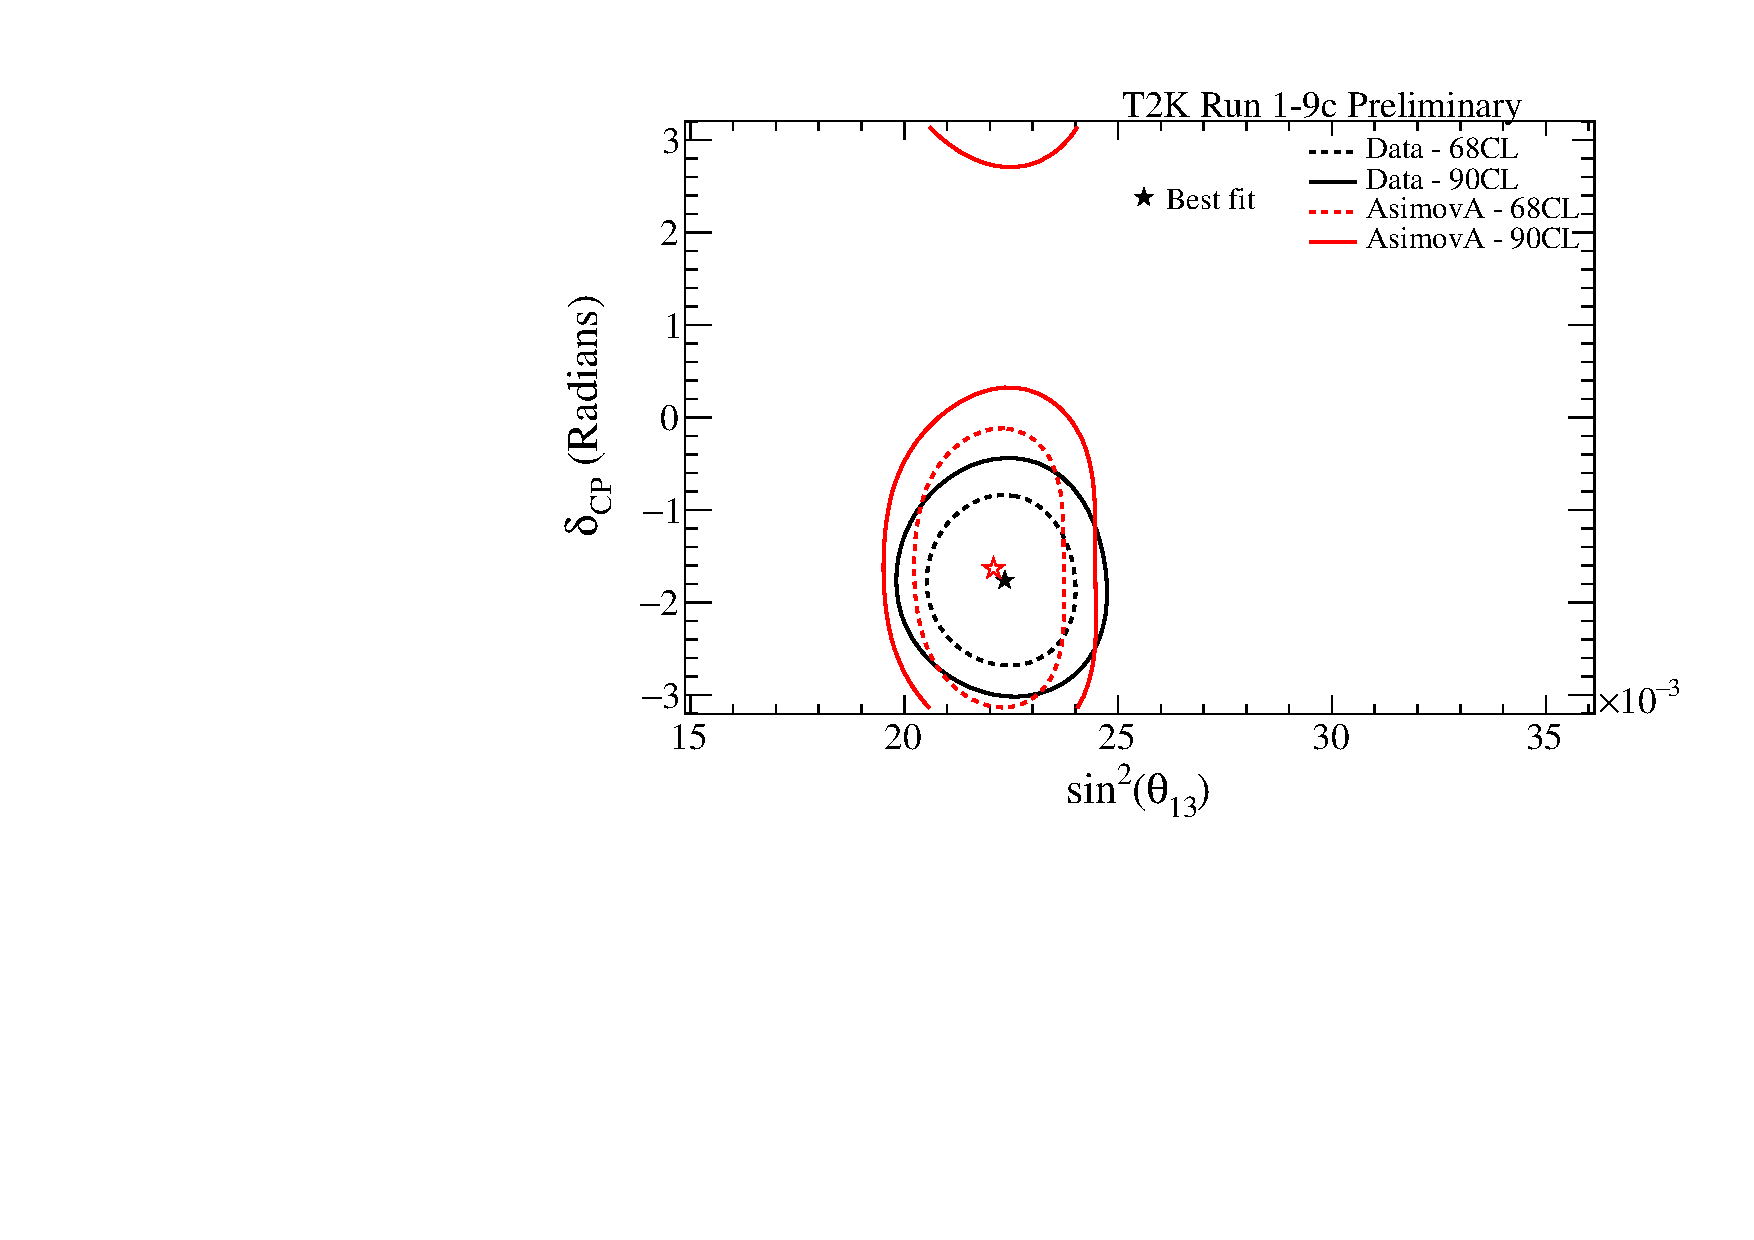
\includegraphics[width=0.9\textwidth]{images/data/asimov_comparison/appearance_wrc_normal_Data_v_AsimovA}
		\caption{\appearance NH with reactor constraint}
	\end{subfigure}
	\begin{subfigure}[b]{0.49\textwidth}
		\includegraphics[width=0.9\textwidth]{images/data/asimov_comparison/appearance_wrc_inverted_Data_v_AsimovA}
		\caption{\appearance IH with reactor constraint}
	\end{subfigure}
	\begin{subfigure}[b]{0.49\textwidth}
		\includegraphics[width=0.9\textwidth]{images/data/asimov_comparison/appearance_worc_normal_Data_v_AsimovA}
		\caption{\appearance NH without reactor constraint}
	\end{subfigure}
	\begin{subfigure}[b]{0.49\textwidth}
		\includegraphics[width=0.9\textwidth]{images/data/asimov_comparison/appearance_worc_inverted_Data_v_AsimovA}
		\caption{\appearance IH without reactor constraint}
	\end{subfigure}
	\caption {
		Contours at 68\% and 90\% CL for \appearance with and without reactor constraint. Normal and inverted hierarchy contours are independent. All 5 samples were used to produce these fits.
	}
	\label{fig:ssqth13_vs_dcp_data_asimov_compare}
\end{figure*}
\clearpage

\subsection{Results for \disappearance}

The result for \disappearance with reactor constraint and T2K only is shown in fig.~\ref{fig:ssqth23_vs_dmsq_data_asimov_compare}.

\begin{figure*}[htb]
	\center
	\begin{subfigure}[b]{0.49\textwidth}
		\includegraphics[width=0.9\textwidth]{images/data/asimov_comparison/disappearance_wrc_normal_Data_v_AsimovA}
		\caption{\disappearance NH with reactor constraint}
	\end{subfigure}
	\begin{subfigure}[b]{0.49\textwidth}
		\includegraphics[width=0.9\textwidth]{images/data/asimov_comparison/disappearance_wrc_inverted_Data_v_AsimovA}
		\caption{\disappearance IH with reactor constraint}
	\end{subfigure}
	\begin{subfigure}[b]{0.49\textwidth}
		\includegraphics[width=0.9\textwidth]{images/data/asimov_comparison/disappearance_worc_normal_Data_v_AsimovA}
		\caption{\disappearance NH without reactor constraint}
	\end{subfigure}
	\begin{subfigure}[b]{0.49\textwidth}
		\includegraphics[width=0.9\textwidth]{images/data/asimov_comparison/disappearance_worc_inverted_Data_v_AsimovA}
		\caption{\disappearance IH without reactor constraint}
	\end{subfigure}
	\caption {
		Contours at 68\% and 90\% CL for \disappearance with and without reactor constraint. Normal and inverted hierarchy contours are independent. All 5 samples were used to produce these fits.
	}
	\label{fig:ssqth23_vs_dmsq_data_asimov_compare}
\end{figure*}

\clearpage

\subsection{Results for \deltacp}

The result for \deltacp with reactor constraint and T2K only is shown in fig.~\ref{fig:dcp_data_asimov_compare}.

\begin{figure*}[htb]
	\center
	\begin{subfigure}[b]{0.49\textwidth}
		\includegraphics[width=0.9\textwidth]{images/data/asimov_comparison/deltacp_wrc_normal_Data_v_AsimovA}
		\caption{\deltacp NH with reactor constraint}
	\end{subfigure}
	\begin{subfigure}[b]{0.49\textwidth}
		\includegraphics[width=0.9\textwidth]{images/data/asimov_comparison/deltacp_wrc_inverted_Data_v_AsimovA}
		\caption{\deltacp IH with reactor constraint}
	\end{subfigure}
	\begin{subfigure}[b]{0.49\textwidth}
		\includegraphics[width=0.9\textwidth]{images/data/asimov_comparison/deltacp_worc_normal_Data_v_AsimovA}
		\caption{\deltacp NH without reactor constraint}
	\end{subfigure}
	\begin{subfigure}[b]{0.49\textwidth}
		\includegraphics[width=0.9\textwidth]{images/data/asimov_comparison/deltacp_worc_inverted_Data_v_AsimovA}
		\caption{\deltacp IH without reactor constraint}
	\end{subfigure}
	\caption {
		The expected $\Delta\chi^2$ distribution as a function of \deltacp with and without reactor constraint. Normal and inverted hierarchy contours are independent. All 5 samples were used to produce these fits.
	}
	\label{fig:dcp_data_asimov_compare}
\end{figure*}
\clearpage

\subsection{Results for \ssqthonethree}

The result for \ssqthonethree (without reactor constraint) is shown in fig.~\ref{fig:th13_data_asimov_compare}.

\begin{figure*}[htb]
	\center
	\begin{subfigure}[b]{0.49\textwidth}
		\includegraphics[width=0.9\textwidth]{images/data/asimov_comparison/theta13_worc_normal_Data_v_AsimovA}
		\caption{\ssqthonethree NH without reactor constraint}
	\end{subfigure}
	\begin{subfigure}[b]{0.49\textwidth}
		\includegraphics[width=0.9\textwidth]{images/data/asimov_comparison/theta13_worc_inverted_Data_v_AsimovA}
		\caption{\ssqthonethree IH without reactor constraint}
	\end{subfigure}
	\caption {
		The expected $\Delta\chi^2$ distribution as a function of \ssqthonethree without reactor constraint. Normal and inverted hierarchy contours are independent. All 5 samples were used to produce these fits.
	}
	\label{fig:th13_data_asimov_compare}
\end{figure*}

\clearpage

\subsection{Results for \ssqthtwothree}

The result for \ssqthtwothree with reactor constraint and T2K only is shown in fig.~\ref{fig:th23_data_asimov_compare}.

\begin{figure*}[htb]
	\center
	\begin{subfigure}[b]{0.49\textwidth}
		\includegraphics[width=0.9\textwidth]{images/data/asimov_comparison/theta23_wrc_normal_Data_v_AsimovA}
		\caption{\ssqthtwothree NH with reactor constraint}
	\end{subfigure}
	\begin{subfigure}[b]{0.49\textwidth}
		\includegraphics[width=0.9\textwidth]{images/data/asimov_comparison/theta23_wrc_inverted_Data_v_AsimovA}
		\caption{\ssqthtwothree IH with reactor constraint}
	\end{subfigure}
	\begin{subfigure}[b]{0.49\textwidth}
		\includegraphics[width=0.9\textwidth]{images/data/asimov_comparison/theta23_worc_normal_Data_v_AsimovA}
		\caption{\ssqthtwothree NH without reactor constraint}
	\end{subfigure}
	\begin{subfigure}[b]{0.49\textwidth}
		\includegraphics[width=0.9\textwidth]{images/data/asimov_comparison/theta23_worc_inverted_Data_v_AsimovA}
		\caption{\ssqthtwothree IH without reactor constraint}
	\end{subfigure}
	\caption {
		The expected $\Delta\chi^2$ distribution as a function of \ssqthtwothree with and without reactor constraint. Normal and inverted hierarchy contours are independent. All 5 samples were used to produce these fits.
	}
	\label{fig:th23_data_asimov_compare}
\end{figure*}
\clearpage

\subsection{Results for \dmsq}

The result for \dmsq with reactor constraint and T2K only is shown in fig.~\ref{fig:dmsq_data_asimov_compare}.

\begin{figure*}[htb]
	\center
	\begin{subfigure}[b]{0.49\textwidth}
		\includegraphics[width=0.9\textwidth]{images/data/asimov_comparison/dmsq_wrc_normal_Data_v_AsimovA}
		\caption{\dmsq NH with reactor constraint}
	\end{subfigure}
	\begin{subfigure}[b]{0.49\textwidth}
		\includegraphics[width=0.9\textwidth]{images/data/asimov_comparison/dmsq_wrc_inverted_Data_v_AsimovA}
		\caption{\dmsq IH with reactor constraint}
	\end{subfigure}
	\begin{subfigure}[b]{0.49\textwidth}
		\includegraphics[width=0.9\textwidth]{images/data/asimov_comparison/dmsq_worc_normal_Data_v_AsimovA}
		\caption{\dmsq NH without reactor constraint}
	\end{subfigure}
	\begin{subfigure}[b]{0.49\textwidth}
		\includegraphics[width=0.9\textwidth]{images/data/asimov_comparison/dmsq_worc_inverted_Data_v_AsimovA}
		\caption{\dmsq IH without reactor constraint}
	\end{subfigure}
	\caption {
		The expected $\Delta\chi^2$ distribution as a function of \dmsqtwothree with and without reactor constraint. Normal and inverted hierarchy contours are independent. All 5 samples were used to produce these fits.
	}
	\label{fig:dmsq_data_asimov_compare}
\end{figure*}

\clearpage
	\clearpage

\section{Comparison of \RunPeriod to \PrevRunPeriod for Asimov A sensitivities}
\label{app:asimov_comparison}

This chapter compares the expected Asimov A sensitivities for the current \RunPeriod to those of the previous \PrevRunPeriod period.

\subsection{Results for \appearance}
In \cref{fig:ssqth13_vs_dcp_asimov_compare} the result for \appearance with reactor constraint and T2K only is shown.

\begin{figure*}[htb]
	\center
	\begin{subfigure}[b]{0.49\textwidth}
		\includegraphics[width=0.9\textwidth]{images/sensitivity/comparison/appearance_wrc_normal_2018_v_2017}
		\caption{\appearance NH with reactor constraint}
	\end{subfigure}
	\begin{subfigure}[b]{0.49\textwidth}
		\includegraphics[width=0.9\textwidth]{images/sensitivity/comparison/appearance_wrc_inverted_2018_v_2017}
		\caption{\appearance IH with reactor constraint}
	\end{subfigure}
	\begin{subfigure}[b]{0.49\textwidth}
		\includegraphics[width=0.9\textwidth]{images/sensitivity/comparison/appearance_worc_normal_2018_v_2017}
		\caption{\appearance NH without reactor constraint}
	\end{subfigure}
	\begin{subfigure}[b]{0.49\textwidth}
		\includegraphics[width=0.9\textwidth]{images/sensitivity/comparison/appearance_worc_inverted_2018_v_2017}
		\caption{\appearance IH without reactor constraint}
	\end{subfigure}
	\caption {
		Contours at 68\% and 90\% CL for \appearance with and without reactor constraint. Normal and inverted hierarchy contours are independent. All 5 samples were used to produce these fits.
	}
	\label{fig:ssqth13_vs_dcp_asimov_compare}
\end{figure*}
\clearpage

\subsection{Results for \disappearance}

The result for \disappearance with reactor constraint and T2K only is shown in fig.~\ref{fig:ssqth23_vs_dmsq_asimov_compare}.

\begin{figure*}[htb]
	\center
	\begin{subfigure}[b]{0.49\textwidth}
		\includegraphics[width=0.9\textwidth]{images/sensitivity/comparison/disappearance_wrc_normal_2018_v_2017}
		\caption{\disappearance NH with reactor constraint}
	\end{subfigure}
	\begin{subfigure}[b]{0.49\textwidth}
		\includegraphics[width=0.9\textwidth]{images/sensitivity/comparison/disappearance_wrc_inverted_2018_v_2017}
		\caption{\disappearance IH with reactor constraint}
	\end{subfigure}
	\begin{subfigure}[b]{0.49\textwidth}
		\includegraphics[width=0.9\textwidth]{images/sensitivity/comparison/disappearance_worc_normal_2018_v_2017}
		\caption{\disappearance NH without reactor constraint}
	\end{subfigure}
	\begin{subfigure}[b]{0.49\textwidth}
		\includegraphics[width=0.9\textwidth]{images/sensitivity/comparison/disappearance_worc_inverted_2018_v_2017}
		\caption{\disappearance IH without reactor constraint}
	\end{subfigure}
	\caption {
		Contours at 68\% and 90\% CL for \disappearance with and without reactor constraint. Normal and inverted hierarchy contours are independent. All 5 samples were used to produce these fits.
	}
	\label{fig:ssqth23_vs_dmsq_asimov_compare}
\end{figure*}

\clearpage

\subsection{Results for \deltacp}

The result for \deltacp with reactor constraint and T2K only is shown in fig.~\ref{fig:dcp_asimov_compare}.

\begin{figure*}[htb]
	\center
	\begin{subfigure}[b]{0.49\textwidth}
		\includegraphics[width=0.9\textwidth]{images/sensitivity/comparison/deltacp_wrc_normal_2018_v_2017}
		\caption{\deltacp NH with reactor constraint}
	\end{subfigure}
	\begin{subfigure}[b]{0.49\textwidth}
		\includegraphics[width=0.9\textwidth]{images/sensitivity/comparison/deltacp_wrc_inverted_2018_v_2017}
		\caption{\deltacp IH with reactor constraint}
	\end{subfigure}
	\begin{subfigure}[b]{0.49\textwidth}
		\includegraphics[width=0.9\textwidth]{images/sensitivity/comparison/deltacp_worc_normal_2018_v_2017}
		\caption{\deltacp NH without reactor constraint}
	\end{subfigure}
	\begin{subfigure}[b]{0.49\textwidth}
		\includegraphics[width=0.9\textwidth]{images/sensitivity/comparison/deltacp_worc_inverted_2018_v_2017}
		\caption{\deltacp IH without reactor constraint}
	\end{subfigure}
	\caption {
		The expected $\Delta\chi^2$ distribution as a function of \deltacp with and without reactor constraint. Normal and inverted hierarchy contours are independent. All 5 samples were used to produce these fits.
	}
	\label{fig:dcp_asimov_compare}
\end{figure*}
\clearpage

\subsection{Results for \ssqthonethree}

The result for \ssqthonethree (without reactor constraint) is shown in fig.~\ref{fig:th13_asimov_compare}.

\begin{figure*}[htb]
	\center
	\begin{subfigure}[b]{0.49\textwidth}
		\includegraphics[width=0.9\textwidth]{images/sensitivity/comparison/theta13_worc_normal_2018_v_2017}
		\caption{\ssqthonethree NH without reactor constraint}
	\end{subfigure}
	\begin{subfigure}[b]{0.49\textwidth}
		\includegraphics[width=0.9\textwidth]{images/sensitivity/comparison/theta13_worc_inverted_2018_v_2017}
		\caption{\ssqthonethree IH without reactor constraint}
	\end{subfigure}
	\caption {
		The expected $\Delta\chi^2$ distribution as a function of \ssqthonethree without reactor constraint. Normal and inverted hierarchy contours are independent. All 5 samples were used to produce these fits.
	}
	\label{fig:th13_asimov_compare}
\end{figure*}

\clearpage

\subsection{Results for \ssqthtwothree}

The result for \ssqthtwothree with reactor constraint and T2K only is shown in fig.~\ref{fig:th23_asimov_compare}.

\begin{figure*}[htb]
	\center
	\begin{subfigure}[b]{0.49\textwidth}
		\includegraphics[width=0.9\textwidth]{images/sensitivity/comparison/theta23_wrc_normal_2018_v_2017}
		\caption{\ssqthtwothree NH with reactor constraint}
	\end{subfigure}
	\begin{subfigure}[b]{0.49\textwidth}
		\includegraphics[width=0.9\textwidth]{images/sensitivity/comparison/theta23_wrc_inverted_2018_v_2017}
		\caption{\ssqthtwothree IH with reactor constraint}
	\end{subfigure}
	\begin{subfigure}[b]{0.49\textwidth}
		\includegraphics[width=0.9\textwidth]{images/sensitivity/comparison/theta23_worc_normal_2018_v_2017}
		\caption{\ssqthtwothree NH without reactor constraint}
	\end{subfigure}
	\begin{subfigure}[b]{0.49\textwidth}
		\includegraphics[width=0.9\textwidth]{images/sensitivity/comparison/theta23_worc_inverted_2018_v_2017}
		\caption{\ssqthtwothree IH without reactor constraint}
	\end{subfigure}
	\caption {
		The expected $\Delta\chi^2$ distribution as a function of \ssqthtwothree with and without reactor constraint. Normal and inverted hierarchy contours are independent. All 5 samples were used to produce these fits.
	}
	\label{fig:th23_asimov_compare}
\end{figure*}
\clearpage

\subsection{Results for \dmsq}

The result for \dmsq with reactor constraint and T2K only is shown in fig.~\ref{fig:dmsq_asimov_compare}.

\begin{figure*}[htb]
	\center
	\begin{subfigure}[b]{0.49\textwidth}
		\includegraphics[width=0.9\textwidth]{images/sensitivity/comparison/dmsq_wrc_normal_2018_v_2017}
		\caption{\dmsq NH with reactor constraint}
	\end{subfigure}
	\begin{subfigure}[b]{0.49\textwidth}
		\includegraphics[width=0.9\textwidth]{images/sensitivity/comparison/dmsq_wrc_inverted_2018_v_2017}
		\caption{\dmsq IH with reactor constraint}
	\end{subfigure}
	\begin{subfigure}[b]{0.49\textwidth}
		\includegraphics[width=0.9\textwidth]{images/sensitivity/comparison/dmsq_worc_normal_2018_v_2017}
		\caption{\dmsq NH without reactor constraint}
	\end{subfigure}
	\begin{subfigure}[b]{0.49\textwidth}
		\includegraphics[width=0.9\textwidth]{images/sensitivity/comparison/dmsq_worc_inverted_2018_v_2017}
		\caption{\dmsq IH without reactor constraint}
	\end{subfigure}
	\caption {
		The expected $\Delta\chi^2$ distribution as a function of \dmsqtwothree with and without reactor constraint. Normal and inverted hierarchy contours are independent. All 5 samples were used to produce these fits.
	}
	\label{fig:dmsq_asimov_compare}
\end{figure*}

\clearpage
	\section{Comparison between different fitting groups}
\label{app:group_comparison}
This appendix compares the fits produced by the MaCh3\cite{MaCh3:2018}, p-theta\cite{ptheta:2018} and VALOR fitting groups.

\subsection{Data fits}

\subsubsection{Results for \appearance}
In \cref{fig:ssqth13_vs_dcp_data_group_compare} the result for \appearance with reactor constraint and T2K only is shown.

\begin{figure*}[htb]
	\center
	\begin{subfigure}[b]{0.49\textwidth}
		\includegraphics[width=0.9\textwidth]{images/data/group_comparison/appearance_wrc_nh_data}
		\caption{\appearance NH with reactor constraint}
	\end{subfigure}
	\begin{subfigure}[b]{0.49\textwidth}
		\includegraphics[width=0.9\textwidth]{images/data/group_comparison/appearance_wrc_ih_data}
		\caption{\appearance IH with reactor constraint}
	\end{subfigure}
	\begin{subfigure}[b]{0.49\textwidth}
		\includegraphics[width=0.9\textwidth]{images/data/group_comparison/appearance_worc_nh_data}
		\caption{\appearance NH without reactor constraint}
	\end{subfigure}
	\begin{subfigure}[b]{0.49\textwidth}
		\includegraphics[width=0.9\textwidth]{images/data/group_comparison/appearance_worc_ih_data}
		\caption{\appearance IH without reactor constraint}
	\end{subfigure}
	\caption {
		Contours at 68\% and 90\% CL for \appearance with and without reactor constraint. Normal and inverted hierarchy contours are independent. All 5 samples were used to produce these fits.
	}
	\label{fig:ssqth13_vs_dcp_data_group_compare}
\end{figure*}
\clearpage

\subsubsection{Results for \disappearance}

The result for \disappearance with reactor constraint and T2K only is shown in fig.~\ref{fig:ssqth23_vs_dmsq_data_group_compare}. The difference between p-theta and the other fitting groups is driven by the difference in variables and binning between the fitters. When p-theta fits the data using the same variables and binning as the other fitting groups, good agreement is observed between p-theta and VALOR.

\begin{figure*}[htb]
	\center
	\begin{subfigure}[b]{0.49\textwidth}
		\includegraphics[width=0.9\textwidth]{images/data/group_comparison/disappearance_wrc_nh_data}
		\caption{\disappearance NH with reactor constraint}
	\end{subfigure}
	\begin{subfigure}[b]{0.49\textwidth}
		\includegraphics[width=0.9\textwidth]{images/data/group_comparison/disappearance_wrc_ih_data}
		\caption{\disappearance IH with reactor constraint}
	\end{subfigure}
	\begin{subfigure}[b]{0.49\textwidth}
		\includegraphics[width=0.9\textwidth]{images/data/group_comparison/disappearance_worc_nh_data}
		\caption{\disappearance NH without reactor constraint}
	\end{subfigure}
	\begin{subfigure}[b]{0.49\textwidth}
		\includegraphics[width=0.9\textwidth]{images/data/group_comparison/disappearance_worc_ih_data}
		\caption{\disappearance IH without reactor constraint}
	\end{subfigure}
	\begin{subfigure}[b]{0.49\textwidth}
		\includegraphics[width=0.9\textwidth]{images/data/group_comparison/disappearance_wrc_nh_ptheta_erec}
		\caption{\disappearance NH with reactor constraint}
	\end{subfigure}
	\begin{subfigure}[b]{0.49\textwidth}
		\includegraphics[width=0.9\textwidth]{images/data/group_comparison/disappearance_wrc_ih_ptheta_erec}
		\caption{\disappearance IH with reactor constraint}
	\end{subfigure}
	\caption {
		Contours at 68\% and 90\% CL for \disappearance with (top) and without (bottom) reactor constraint and comparison to p-theta reactor fit with $E_r-\theta$ templates (bottom). Normal and inverted hierarchy contours are independent. All 5 samples were used to produce these fits.
	}
	\label{fig:ssqth23_vs_dmsq_data_group_compare}
\end{figure*}

\clearpage

\subsubsection{Results for \deltacp}

The result for \deltacp with reactor constraint and T2K only is shown in fig.~\ref{fig:dcp_data_group_compare}.

\begin{figure*}[htb]
	\center
	\begin{subfigure}[b]{0.49\textwidth}
		\includegraphics[width=0.9\textwidth]{images/data/group_comparison/deltacp_wrc_nh_data}
		\caption{\deltacp NH with reactor constraint}
	\end{subfigure}
	\begin{subfigure}[b]{0.49\textwidth}
		\includegraphics[width=0.9\textwidth]{images/data/group_comparison/deltacp_wrc_ih_data}
		\caption{\deltacp IH with reactor constraint}
	\end{subfigure}
	\begin{subfigure}[b]{0.49\textwidth}
		\includegraphics[width=0.9\textwidth]{images/data/group_comparison/deltacp_worc_nh_data}
		\caption{\deltacp NH without reactor constraint}
	\end{subfigure}
	\begin{subfigure}[b]{0.49\textwidth}
		\includegraphics[width=0.9\textwidth]{images/data/group_comparison/deltacp_worc_ih_data}
		\caption{\deltacp IH without reactor constraint}
	\end{subfigure}
	\caption {
		The expected $\Delta\chi^2$ distribution as a function of \deltacp with and without reactor constraint. Normal and inverted hierarchy contours are independent. All 5 samples were used to produce these fits.
	}
	\label{fig:dcp_data_group_compare}
\end{figure*}
\clearpage

\subsubsection{Results for \ssqthonethree}

The result for \ssqthonethree (without reactor constraint) is shown in fig.~\ref{fig:th13_data_group_compare}.

\begin{figure*}[htb]
	\center
	\begin{subfigure}[b]{0.49\textwidth}
		\includegraphics[width=0.9\textwidth]{images/data/group_comparison/theta13_worc_nh_data}
		\caption{\ssqthonethree NH without reactor constraint}
	\end{subfigure}
	\begin{subfigure}[b]{0.49\textwidth}
		\includegraphics[width=0.9\textwidth]{images/data/group_comparison/theta13_worc_ih_data}
		\caption{\ssqthonethree IH without reactor constraint}
	\end{subfigure}
	\caption {
		The expected $\Delta\chi^2$ distribution as a function of \ssqthonethree without reactor constraint. Normal and inverted hierarchy contours are independent. All 5 samples were used to produce these fits.
	}
	\label{fig:th13_data_group_compare}
\end{figure*}

\clearpage

\subsubsection{Results for \ssqthtwothree}

The result for \ssqthtwothree with reactor constraint and T2K only is shown in fig.~\ref{fig:th23_data_group_compare}.

\begin{figure*}[htb]
	\center
	\begin{subfigure}[b]{0.49\textwidth}
		\includegraphics[width=0.9\textwidth]{images/data/group_comparison/theta23_wrc_nh_data}
		\caption{\ssqthtwothree NH with reactor constraint}
	\end{subfigure}
	\begin{subfigure}[b]{0.49\textwidth}
		\includegraphics[width=0.9\textwidth]{images/data/group_comparison/theta23_wrc_ih_data}
		\caption{\ssqthtwothree IH with reactor constraint}
	\end{subfigure}
	\begin{subfigure}[b]{0.49\textwidth}
		\includegraphics[width=0.9\textwidth]{images/data/group_comparison/theta23_worc_nh_data}
		\caption{\ssqthtwothree NH without reactor constraint}
	\end{subfigure}
	\begin{subfigure}[b]{0.49\textwidth}
		\includegraphics[width=0.9\textwidth]{images/data/group_comparison/theta23_worc_ih_data}
		\caption{\ssqthtwothree IH without reactor constraint}
	\end{subfigure}
	\caption {
		The expected $\Delta\chi^2$ distribution as a function of \ssqthtwothree with and without reactor constraint. Normal and inverted hierarchy contours are independent. All 5 samples were used to produce these fits.
	}
	\label{fig:th23_data_group_compare}
\end{figure*}
\clearpage

\subsubsection{Results for \dmsq}

The result for \dmsq with reactor constraint and T2K only is shown in fig.~\ref{fig:dmsq_data_group_compare}.

\begin{figure*}[htb]
	\center
	\begin{subfigure}[b]{0.49\textwidth}
		\includegraphics[width=0.9\textwidth]{images/data/group_comparison/dmsq_wrc_nh_data}
		\caption{\dmsq NH with reactor constraint}
	\end{subfigure}
	\begin{subfigure}[b]{0.49\textwidth}
		\includegraphics[width=0.9\textwidth]{images/data/group_comparison/dmsq_wrc_ih_data}
		\caption{\dmsq IH with reactor constraint}
	\end{subfigure}
	\begin{subfigure}[b]{0.49\textwidth}
		\includegraphics[width=0.9\textwidth]{images/data/group_comparison/dmsq_worc_nh_data}
		\caption{\dmsq NH without reactor constraint}
	\end{subfigure}
	\begin{subfigure}[b]{0.49\textwidth}
		\includegraphics[width=0.9\textwidth]{images/data/group_comparison/dmsq_worc_ih_data}
		\caption{\dmsq IH without reactor constraint}
	\end{subfigure}
	\caption {
		The expected $\Delta\chi^2$ distribution as a function of \dmsqtwothree with and without reactor constraint. Normal and inverted hierarchy contours are independent. All 5 samples were used to produce these fits.
	}
	\label{fig:dmsq_data_group_compare}
\end{figure*}
\FloatBarrier
\clearpage

\subsection{Asimov A fits}

\subsubsection{Results for \appearance}
In \cref{fig:ssqth13_vs_dcp_asimova_group_compare} the result for \appearance with reactor constraint and T2K only is shown.

\begin{figure*}[htb]
	\center
	\begin{subfigure}[b]{0.49\textwidth}
		\includegraphics[width=0.9\textwidth]{images/sensitivity/group_comparison/appearance_wrc_nh_asimova}
		\caption{\appearance NH with reactor constraint}
	\end{subfigure}
	\begin{subfigure}[b]{0.49\textwidth}
		\includegraphics[width=0.9\textwidth]{images/sensitivity/group_comparison/appearance_wrc_ih_asimova}
		\caption{\appearance IH with reactor constraint}
	\end{subfigure}
	\begin{subfigure}[b]{0.49\textwidth}
		\includegraphics[width=0.9\textwidth]{images/sensitivity/group_comparison/appearance_worc_nh_asimova}
		\caption{\appearance NH without reactor constraint}
	\end{subfigure}
	\begin{subfigure}[b]{0.49\textwidth}
		\includegraphics[width=0.9\textwidth]{images/sensitivity/group_comparison/appearance_worc_ih_asimova}
		\caption{\appearance IH without reactor constraint}
	\end{subfigure}
	\caption {
		Contours at 68\% and 90\% CL for \appearance with and without reactor constraint. Normal and inverted hierarchy contours are independent. All 5 samples were used to produce these fits.
	}
	\label{fig:ssqth13_vs_dcp_asimova_group_compare}
\end{figure*}
\clearpage

\subsubsection{Results for \disappearance}

The result for \disappearance with reactor constraint and T2K only is shown in fig.~\ref{fig:ssqth23_vs_dmsq_asimova_group_compare}.

\begin{figure*}[htb]
	\center
	\begin{subfigure}[b]{0.49\textwidth}
		\includegraphics[width=0.9\textwidth]{images/sensitivity/group_comparison/disappearance_wrc_nh_asimova}
		\caption{\disappearance NH with reactor constraint}
	\end{subfigure}
	\begin{subfigure}[b]{0.49\textwidth}
		\includegraphics[width=0.9\textwidth]{images/sensitivity/group_comparison/disappearance_wrc_ih_asimova}
		\caption{\disappearance IH with reactor constraint}
	\end{subfigure}
	\begin{subfigure}[b]{0.49\textwidth}
		\includegraphics[width=0.9\textwidth]{images/sensitivity/group_comparison/disappearance_worc_nh_asimova}
		\caption{\disappearance NH without reactor constraint}
	\end{subfigure}
	\begin{subfigure}[b]{0.49\textwidth}
		\includegraphics[width=0.9\textwidth]{images/sensitivity/group_comparison/disappearance_worc_ih_asimova}
		\caption{\disappearance IH without reactor constraint}
	\end{subfigure}
	\caption {
		Contours at 68\% and 90\% CL for \disappearance with and without reactor constraint. Normal and inverted hierarchy contours are independent. All 5 samples were used to produce these fits.
	}
	\label{fig:ssqth23_vs_dmsq_asimova_group_compare}
\end{figure*}
\clearpage

\subsubsection{Results for \deltacp}

The result for \deltacp with reactor constraint and T2K only is shown in fig.~\ref{fig:dcp_asimova_group_compare}.

\begin{figure*}[htb]
	\center
	\begin{subfigure}[b]{0.49\textwidth}
		\includegraphics[width=0.9\textwidth]{images/sensitivity/group_comparison/deltacp_wrc_nh_asimova}
		\caption{\deltacp NH with reactor constraint}
	\end{subfigure}
	\begin{subfigure}[b]{0.49\textwidth}
		\includegraphics[width=0.9\textwidth]{images/sensitivity/group_comparison/deltacp_wrc_ih_asimova}
		\caption{\deltacp IH with reactor constraint}
	\end{subfigure}
	\begin{subfigure}[b]{0.49\textwidth}
		\includegraphics[width=0.9\textwidth]{images/sensitivity/group_comparison/deltacp_worc_nh_asimova}
		\caption{\deltacp NH without reactor constraint}
	\end{subfigure}
	\begin{subfigure}[b]{0.49\textwidth}
		\includegraphics[width=0.9\textwidth]{images/sensitivity/group_comparison/deltacp_worc_ih_asimova}
		\caption{\deltacp IH without reactor constraint}
	\end{subfigure}
	\caption {
		The expected $\Delta\chi^2$ distribution as a function of \deltacp with and without reactor constraint. Normal and inverted hierarchy contours are independent. All 5 samples were used to produce these fits.
	}
	\label{fig:dcp_asimova_group_compare}
\end{figure*}
\clearpage

\subsubsection{Results for \ssqthonethree}

The result for \ssqthonethree (without reactor constraint) is shown in fig.~\ref{fig:th13_asimova_group_compare}.

\begin{figure*}[htb]
	\center
	\begin{subfigure}[b]{0.49\textwidth}
		\includegraphics[width=0.9\textwidth]{images/sensitivity/group_comparison/theta13_worc_nh_asimova}
		\caption{\ssqthonethree NH without reactor constraint}
	\end{subfigure}
	\begin{subfigure}[b]{0.49\textwidth}
		\includegraphics[width=0.9\textwidth]{images/sensitivity/group_comparison/theta13_worc_ih_asimova}
		\caption{\ssqthonethree IH without reactor constraint}
	\end{subfigure}
	\caption {
		The expected $\Delta\chi^2$ distribution as a function of \ssqthonethree without reactor constraint. Normal and inverted hierarchy contours are independent. All 5 samples were used to produce these fits.
	}
	\label{fig:th13_asimova_group_compare}
\end{figure*}

\clearpage

\subsubsection{Results for \ssqthtwothree}

The result for \ssqthtwothree with reactor constraint and T2K only is shown in fig.~\ref{fig:th23_asimova_group_compare}.

\begin{figure*}[htb]
	\center
	\begin{subfigure}[b]{0.49\textwidth}
		\includegraphics[width=0.9\textwidth]{images/sensitivity/group_comparison/theta23_wrc_nh_asimova}
		\caption{\ssqthtwothree NH with reactor constraint}
	\end{subfigure}
	\begin{subfigure}[b]{0.49\textwidth}
		\includegraphics[width=0.9\textwidth]{images/sensitivity/group_comparison/theta23_wrc_ih_asimova}
		\caption{\ssqthtwothree IH with reactor constraint}
	\end{subfigure}
	\begin{subfigure}[b]{0.49\textwidth}
		\includegraphics[width=0.9\textwidth]{images/sensitivity/group_comparison/theta23_worc_nh_asimova}
		\caption{\ssqthtwothree NH without reactor constraint}
	\end{subfigure}
	\begin{subfigure}[b]{0.49\textwidth}
		\includegraphics[width=0.9\textwidth]{images/sensitivity/group_comparison/theta23_worc_ih_asimova}
		\caption{\ssqthtwothree IH without reactor constraint}
	\end{subfigure}
	\caption {
		The expected $\Delta\chi^2$ distribution as a function of \ssqthtwothree with and without reactor constraint. Normal and inverted hierarchy contours are independent. All 5 samples were used to produce these fits.
	}
	\label{fig:th23_asimova_group_compare}
\end{figure*}
\clearpage

\subsubsection{Results for \dmsq}

The result for \dmsq with reactor constraint and T2K only is shown in fig.~\ref{fig:dmsq_asimova_group_compare}.

\begin{figure*}[htb]
	\center
	\begin{subfigure}[b]{0.49\textwidth}
		\includegraphics[width=0.9\textwidth]{images/sensitivity/group_comparison/dmsq_wrc_nh_asimova}
		\caption{\dmsq NH with reactor constraint}
	\end{subfigure}
	\begin{subfigure}[b]{0.49\textwidth}
		\includegraphics[width=0.9\textwidth]{images/sensitivity/group_comparison/dmsq_wrc_ih_asimova}
		\caption{\dmsq IH with reactor constraint}
	\end{subfigure}
	\begin{subfigure}[b]{0.49\textwidth}
		\includegraphics[width=0.9\textwidth]{images/sensitivity/group_comparison/dmsq_worc_nh_asimova}
		\caption{\dmsq NH without reactor constraint}
	\end{subfigure}
	\begin{subfigure}[b]{0.49\textwidth}
		\includegraphics[width=0.9\textwidth]{images/sensitivity/group_comparison/dmsq_worc_ih_asimova}
		\caption{\dmsq IH without reactor constraint}
	\end{subfigure}
	\caption {
		The expected $\Delta\chi^2$ distribution as a function of \dmsqtwothree with and without reactor constraint. Normal and inverted hierarchy contours are independent. All 5 samples were used to produce these fits.
	}
	\label{fig:dmsq_asimova_group_compare}
\end{figure*}
\FloatBarrier
\clearpage

\subsection{Asimov B fits}

\subsubsection{Results for \appearance}
In \cref{fig:ssqth13_vs_dcp_asimovb_group_compare} the result for \appearance with reactor constraint and T2K only is shown.

\begin{figure*}[htb]
	\center
	\begin{subfigure}[b]{0.49\textwidth}
		\includegraphics[width=0.9\textwidth]{images/sensitivity/group_comparison/appearance_wrc_nh_asimovb}
		\caption{\appearance NH with reactor constraint}
	\end{subfigure}
	\begin{subfigure}[b]{0.49\textwidth}
		\includegraphics[width=0.9\textwidth]{images/sensitivity/group_comparison/appearance_wrc_ih_asimovb}
		\caption{\appearance IH with reactor constraint}
	\end{subfigure}
	\begin{subfigure}[b]{0.49\textwidth}
		\includegraphics[width=0.9\textwidth]{images/sensitivity/group_comparison/appearance_worc_nh_asimovb}
		\caption{\appearance NH without reactor constraint}
	\end{subfigure}
	\begin{subfigure}[b]{0.49\textwidth}
		\includegraphics[width=0.9\textwidth]{images/sensitivity/group_comparison/appearance_worc_ih_asimovb}
		\caption{\appearance IH without reactor constraint}
	\end{subfigure}
	\caption {
		Contours at 68\% and 90\% CL for \appearance with and without reactor constraint. Normal and inverted hierarchy contours are independent. All 5 samples were used to produce these fits.
	}
	\label{fig:ssqth13_vs_dcp_asimovb_group_compare}
\end{figure*}
\clearpage

\subsubsection{Results for \disappearance}

The result for \disappearance with reactor constraint and T2K only is shown in fig.~\ref{fig:ssqth23_vs_dmsq_asimovb_group_compare}.

\begin{figure*}[htb]
	\center
	\begin{subfigure}[b]{0.49\textwidth}
		\includegraphics[width=0.9\textwidth]{images/sensitivity/group_comparison/disappearance_wrc_nh_asimovb}
		\caption{\disappearance NH with reactor constraint}
	\end{subfigure}
	\begin{subfigure}[b]{0.49\textwidth}
		\includegraphics[width=0.9\textwidth]{images/sensitivity/group_comparison/disappearance_wrc_ih_asimovb}
		\caption{\disappearance IH with reactor constraint}
	\end{subfigure}
	\begin{subfigure}[b]{0.49\textwidth}
		\includegraphics[width=0.9\textwidth]{images/sensitivity/group_comparison/disappearance_worc_nh_asimovb}
		\caption{\disappearance NH without reactor constraint}
	\end{subfigure}
	\begin{subfigure}[b]{0.49\textwidth}
		\includegraphics[width=0.9\textwidth]{images/sensitivity/group_comparison/disappearance_worc_ih_asimovb}
		\caption{\disappearance IH without reactor constraint}
	\end{subfigure}
	\caption {
		Contours at 68\% and 90\% CL for \disappearance with and without reactor constraint. Normal and inverted hierarchy contours are independent. All 5 samples were used to produce these fits.
	}
	\label{fig:ssqth23_vs_dmsq_asimovb_group_compare}
\end{figure*}
\clearpage

\subsubsection{Results for \deltacp}

The result for \deltacp with reactor constraint and T2K only is shown in fig.~\ref{fig:dcp_asimovb_group_compare}.

\begin{figure*}[htb]
	\center
	\begin{subfigure}[b]{0.49\textwidth}
		\includegraphics[width=0.9\textwidth]{images/sensitivity/group_comparison/deltacp_wrc_nh_asimovb}
		\caption{\deltacp NH with reactor constraint}
	\end{subfigure}
	\begin{subfigure}[b]{0.49\textwidth}
		\includegraphics[width=0.9\textwidth]{images/sensitivity/group_comparison/deltacp_wrc_ih_asimovb}
		\caption{\deltacp IH with reactor constraint}
	\end{subfigure}
	\begin{subfigure}[b]{0.49\textwidth}
		\includegraphics[width=0.9\textwidth]{images/sensitivity/group_comparison/deltacp_worc_nh_asimovb}
		\caption{\deltacp NH without reactor constraint}
	\end{subfigure}
	\begin{subfigure}[b]{0.49\textwidth}
		\includegraphics[width=0.9\textwidth]{images/sensitivity/group_comparison/deltacp_worc_ih_asimovb}
		\caption{\deltacp IH without reactor constraint}
	\end{subfigure}
	\caption {
		The expected $\Delta\chi^2$ distribution as a function of \deltacp with and without reactor constraint. Normal and inverted hierarchy contours are independent. All 5 samples were used to produce these fits.
	}
	\label{fig:dcp_asimovb_group_compare}
\end{figure*}
\clearpage

\subsubsection{Results for \ssqthonethree}

The result for \ssqthonethree (without reactor constraint) is shown in fig.~\ref{fig:th13_asimovb_group_compare}.

\begin{figure*}[htb]
	\center
	\begin{subfigure}[b]{0.49\textwidth}
		\includegraphics[width=0.9\textwidth]{images/sensitivity/group_comparison/theta13_worc_nh_asimovb}
		\caption{\ssqthonethree NH without reactor constraint}
	\end{subfigure}
	\begin{subfigure}[b]{0.49\textwidth}
		\includegraphics[width=0.9\textwidth]{images/sensitivity/group_comparison/theta13_worc_ih_asimovb}
		\caption{\ssqthonethree IH without reactor constraint}
	\end{subfigure}
	\caption {
		The expected $\Delta\chi^2$ distribution as a function of \ssqthonethree without reactor constraint. Normal and inverted hierarchy contours are independent. All 5 samples were used to produce these fits.
	}
	\label{fig:th13_asimovb_group_compare}
\end{figure*}

\clearpage

\subsubsection{Results for \ssqthtwothree}

The result for \ssqthtwothree with reactor constraint and T2K only is shown in fig.~\ref{fig:th23_asimovb_group_compare}.

\begin{figure*}[htb]
	\center
	\begin{subfigure}[b]{0.49\textwidth}
		\includegraphics[width=0.9\textwidth]{images/sensitivity/group_comparison/theta23_wrc_nh_asimovb}
		\caption{\ssqthtwothree NH with reactor constraint}
	\end{subfigure}
	\begin{subfigure}[b]{0.49\textwidth}
		\includegraphics[width=0.9\textwidth]{images/sensitivity/group_comparison/theta23_wrc_ih_asimovb}
		\caption{\ssqthtwothree IH with reactor constraint}
	\end{subfigure}
	\begin{subfigure}[b]{0.49\textwidth}
		\includegraphics[width=0.9\textwidth]{images/sensitivity/group_comparison/theta23_worc_nh_asimovb}
		\caption{\ssqthtwothree NH without reactor constraint}
	\end{subfigure}
	\begin{subfigure}[b]{0.49\textwidth}
		\includegraphics[width=0.9\textwidth]{images/sensitivity/group_comparison/theta23_worc_ih_asimovb}
		\caption{\ssqthtwothree IH without reactor constraint}
	\end{subfigure}
	\caption {
		The expected $\Delta\chi^2$ distribution as a function of \ssqthtwothree with and without reactor constraint. Normal and inverted hierarchy contours are independent. All 5 samples were used to produce these fits.
	}
	\label{fig:th23_asimovb_group_compare}
\end{figure*}
\clearpage

\subsubsection{Results for \dmsq}

The result for \dmsq with reactor constraint and T2K only is shown in fig.~\ref{fig:dmsq_asimovb_group_compare}.

\begin{figure*}[htb]
	\center
	\begin{subfigure}[b]{0.49\textwidth}
		\includegraphics[width=0.9\textwidth]{images/sensitivity/group_comparison/dmsq_wrc_nh_asimovb}
		\caption{\dmsq NH with reactor constraint}
	\end{subfigure}
	\begin{subfigure}[b]{0.49\textwidth}
		\includegraphics[width=0.9\textwidth]{images/sensitivity/group_comparison/dmsq_wrc_ih_asimovb}
		\caption{\dmsq IH with reactor constraint}
	\end{subfigure}
	\begin{subfigure}[b]{0.49\textwidth}
		\includegraphics[width=0.9\textwidth]{images/sensitivity/group_comparison/dmsq_worc_nh_asimovb}
		\caption{\dmsq NH without reactor constraint}
	\end{subfigure}
	\begin{subfigure}[b]{0.49\textwidth}
		\includegraphics[width=0.9\textwidth]{images/sensitivity/group_comparison/dmsq_worc_ih_asimovb}
		\caption{\dmsq IH without reactor constraint}
	\end{subfigure}
	\caption {
		The expected $\Delta\chi^2$ distribution as a function of \dmsqtwothree with and without reactor constraint. Normal and inverted hierarchy contours are independent. All 5 samples were used to produce these fits.
	}
	\label{fig:dmsq_asimovb_group_compare}
\end{figure*}
\FloatBarrier
\clearpage
	\section{Feldman-Cousins comparison with p-theta}
\label{app:fc_compare}

This section presents comparisons of VALOR and p-theta Feldman-Cousins results. In particular \cref{fig:fc_cv_compare} shows the critical values obtained by each group, whilst \cref{app:fc_compare} shows the $2\sigma$ intervals. p-theta excludes inverted hierarchy at $2\sigma$, whilst VALOR has a small region that is not excluded. This difference is driven not by the small differences in critical values in this region, but by the higher inverted hierarchy minimum seen by p-theta with respect to the global minimum (see top row of \cref{fig:fc_interval_compare}). This difference comes from the different templates used by the two fitters; when p-theta uses the same templates as VALOR, better agreement is observed for the contours (see bottom row of \cref{fig:fc_interval_compare}).

\begin{figure*}[htb]
	\center
	\begin{subfigure}[b]{\textwidth}
		\center
		\includegraphics[width=0.68\textwidth, page=1]{images/fc/fc_compare}
		\caption{NH}
	\end{subfigure}
	\begin{subfigure}[b]{\textwidth}
		\center
		\includegraphics[width=0.68\textwidth, page=2]{images/fc/fc_compare}
		\caption{IH}
	\end{subfigure}
	\caption {
		Feldman-Cousins critical values.
	}
	\label{fig:fc_cv_compare}
\end{figure*}

\begin{figure*}[htb]
	\center
	\begin{subfigure}[b]{0.49\textwidth}
		\center
		\includegraphics[width=\textwidth]{images/fc/deltacp_fc_nh_global}
		\caption{NH, with p-theta using $p-\theta$ template}
	\end{subfigure}
	\begin{subfigure}[b]{0.49\textwidth}
		\center
		\includegraphics[width=\textwidth]{images/fc/deltacp_fc_ih_global}
		\caption{IH, with p-theta using $p-\theta$ template}
	\end{subfigure}
	\begin{subfigure}[b]{0.49\textwidth}
		\center
		\includegraphics[width=\textwidth]{images/fc/deltacp_wrc_nh_ptheta_erec}
		\caption{NH, with p-theta using $E_r-\theta$ template}
	\end{subfigure}
	\begin{subfigure}[b]{0.49\textwidth}
		\center
		\includegraphics[width=\textwidth]{images/fc/deltacp_wrc_ih_ptheta_erec}
		\caption{IH, with p-theta using $E_r-\theta$ template}
	\end{subfigure}
	\caption {
		\deltacp contours with Feldman-Cousins $2\sigma$ critical values. p-theta contours are computed for $p-\theta$ and $E_r-\theta$ templates, but critical values are only computed for $p-\theta$ templates.
	}
	\label{fig:fc_interval_compare}
\end{figure*}

\clearpage
\end{appendices}

\clearpage

\end{document}

%%% Local Variables:
%%% mode: latex
%%% TeX-master: t
%%% End:
